\documentclass[a4paper,twocolumn,openany,10pt]{dndbook}

\usepackage[spanish]{babel}

\usepackage[utf8]{inputenc}
\usepackage{subfig}
\usepackage[singlelinecheck=false]{caption}
\usepackage{lipsum}
\usepackage{listings}
\usepackage{shortvrb}
\usepackage{stfloats}
\setcounter{chapter}{-1}
\usepackage{hyperref}
\usepackage{longtable}

\captionsetup[table]{labelformat=empty,font={sf,sc,bf,},skip=0pt}
\MakeShortVerb{|}

\lstset{%
  basicstyle=\ttfamily,
  language=[LaTeX]{TeX},
  breaklines=true,
}

\title{Guía del Xanathar para Todo \\
\large DnD 5e}
\author{J.E.R.}


\begin{document}

\frontmatter

\maketitle

\tableofcontents

\mainmatter%

\newpage

\chapter{INTRODUCION}

\DndDropCapLine{B}{ebajo de la bulliciosa ciudad de} Waterdeep, un señor del crimen vigila a todo el mundo y a todos,
o eso es lo que piensa el espectador. Conocido como Xanathar, este extraño ser cree que puede reunir información sobre
todo en el multiverso DUNGEONS \& DRAGONS. El ser holder desea saberlo todo! Pero no importa lo que el espectador aprenda
y los tesoros que adquiera, su posesión más preciada es el multiverso que queda en su pez dorado, Sylgar.

\section{Usando este libro}
Escrito tanto para jugadores como para Dungeon Masters, este libro ofrece opciones para mejorar las campañas en cualquier
mundo, ya sea que estés aventurándote en los Reinos Olvidados, en otro escenario oficial de DnD o en un mundo de tu propia
creación. Las opciones aquí se basan en las reglas oficiales contenidas en el Manual del Jugador, el Manual del Monstruo y la
Guía del Maestro del Calabozo. Piense en este libro como el acompañante de esos volúmenes. Se basa en sus cimientos, explorando
los caminos que se establecieron por primera vez en esas publicaciones.

No se requiere nada de esto para una campaña de DnD -esto no es un cuarto libro de reglas- pero esperamos que le proporcione
nuevas formas de disfrutar del juego.

El Capítulo 1 ofrece opciones de caracteres que amplían las que se ofrecen en el Manual del Jugador. El Capítulo 2 es un juego 
de herramientas para el DM que proporciona nuevos recursos para ejecutar el juego y diseñar aventuras, todo ello basado en el
Manual del Monstruo y la Guía del Maestro del Calabozo. El capítulo 3 presenta nuevos conjuros para que los personajes de los
jugadores y los monstruos hechiceros los desaten.

El Apéndice A proporciona una guía para llevar a cabo una campaña compartida, similar a las actividades organizadas por la Liga
de Aventureros de DnD, y el Apéndice B contiene una gran cantidad de tablas que le permitirán generar rápidamente nombres para
los personajes de sus historias de DnD.

A medida que usted se apacigua de las muchas opciones aquí, usted vendrá a través de las observaciones del propio Xanathar. Como
el la mente errante del espectador, tu lectura te llevará a lugares en el juego familiares y nuevos. Que disfrutes el viaje!

\begin{paperbox}[float=!b]{Unartthed Arcana}
Gran parte del material de este libro aparece originalmente en Unearthed Arcana, una serie de artículos en línea que publicamos
para explorar las reglas que podrían convertirse oficialmente en parte del juego. Algunas de las ofertas de Arcanos sin conexión 
a tierra no terminan resonando entre los fans y se dejan de lado por el momento.

El material de los Arcanos Inexplotados que inspiró las opciones de los siguientes capítulos fue bien recibido y gracias a de 
miles de ustedes, ha sido refinada en el formularios oficiales presentados aquí. 
\end{paperbox}

\section{Las reglas basicas}

Este libro se basa en las reglas de los tres libros básicos. El juego hace uso frecuente de las reglas de los capítulos 7 a 10
del Manual del Jugador: ''Usando puntuaciones de habilidad'', ''Aventura'', ''Combate'' y ''Hechicería''. Ese libro es un
apéndice A que también es crucial; contiene definiciones de condiciones, como invisibles y propensas. Usted no necesita saber las
reglas de memoria, pero es útil saber dónde encontrarlas cuando las necesite.

Si eres un DM, también deberías saber dónde buscar cosas en la Guía del Maestro del Calabozo, especialmente las reglas sobre cómo
funcionan los objetos mágicos (ver capítulo 7 de ese libro). La introducción del Manual del Monstruo es tu guía sobre cómo usar el
bloque de estadísticas de un monstruo.

\subsection{El DM dicta las reglas}

Una regla prevalece sobre todas las demás: el DM es la autoridad final sobre cómo funcionan las reglas en juego.

Las reglas son parte de lo que hace de DnD un juego, en lugar de simplemente contar historias improvisadas. Las reglas del juego
están pensadas para ayudar a organizar, e incluso inspirar, la acción de una campaña de DnD. Las reglas son una herramienta, y
queremos que nuestras herramientas sean lo más eficaces posible. No importa lo buenas que sean esas herramientas, necesitan un
grupo de jugadores para darles vida y un DM para guiar su uso.

El DM es clave, muchos eventos inesperados pueden ocurrir en una campaña de DnD, y ningún conjunto de reglas podría explicar
razonablemente cada contingencia. Si las reglas trataban de hacerlo, el juego se convertiría en una carga. Una alternativa sería
que las reglas limiten severamente lo que los personajes pueden hacer, lo que sería contrario a la naturaleza abierta de DnD.
Este es el camino que sigue el juego: establece una base de reglas sobre las que un DM puede construir, y adopta el papel del DM
como puente entre las cosas que las reglas abordan y las que no.

\subsection{Dies reglas para recordar}
Unas pocas reglas en los libros de reglas básicas a veces hacen tropezar a un nuevo jugador o DM. Aquí están diez de esas reglas.
Tenerlos en cuenta le ayudará a interpretar las opciones de este libro.  

\subsubsection{Las excepciones sustituyen a las reglas generales}
Las reglas generales rigen cada parte del juego. Por ejemplo, las reglas de combate te dicen que los ataques con armas cuerpo a
cuerpo usan Fuerza y los ataques con armas a distancia usan Destreza. Esa es una regla general, y una regla general está en vigor
siempre y cuando algo en el juego no diga explícitamente lo contrario.

El juego también incluye elementos -características de clase, conjuros, objetos mágicos, monstruos y cosas por el estilo- que a
veces contradicen una regla general. Cuando una excepción y una regla general no están de acuerdo, la excepción gana. Por ejemplo
si una característica dice que puedes hacer ataques con armas cuerpo a cuerpo usando tu carisma, puedes hacerlo, aunque esa
afirmación no esté de acuerdo con la regla general.

\subsubsection{Redondea hacia abajo}
Siempre que dividas o multipliques un número en el juego, redondea hacia abajo si terminas con una fracción, incluso si la
fracción es la mitad o más

\subsubsection{Ventajas y  desventajas}
Incluso si más de un factor te da ventaja o desventaja en una tirada, sólo lo tienes una vez, y si tienes ventaja y desventaja en
la misma tirada, se cancelan entre sí.

\subsubsection{Combinando diferentes efectos}
Diferentes efectos del juego pueden afectar a un objetivo al mismo tiempo. Por ejemplo, dos beneficios diferentes pueden darle un
bono a su CA. Pero cuando dos o más efectos tienen el mismo nombre propio, sólo uno de ellos (el más potente si sus beneficios no
son idénticos) se aplica mientras que las duraciones de los efectos se superponen. Por ejemplo, si la bendición es arrojada sobre
ti cuando todavía estás bajo el efecto de una bendición anterior, obtienes el beneficio de un solo lanzamiento. Del mismo modo,
si estás en el radio de más de un aura de protección, sólo te beneficias del que te otorga el bono más alto.

\subsubsection{Tiempo de reaccion}
Ciertas características del juego te permiten tomar una acción especial, llamada reacción, en respuesta a algún evento. Hacer
ataques de oportunidad y lanzar el conjuro de escudo son dos usos típicos de las reacciones. Si no está seguro de cuándo se
produce una reacción en relación con su desencadenante, esta es la regla: la reacción se produce después de que se completa su
desencadenante, a menos que la descripción de la reacción diga explícitamente lo contrario.

Una vez que tomas una reacción, no puedes tomar otra hasta el comienzo de tu próximo turno.

\subsubsection{Resistencias y vulnerabilidades}
Aquí está la orden de aplicar modificadores a los daños: (1) cualquier inmunidad pertinente al daño, (2) cualquier suma o resta
al daño, (3) una resistencia pertinente al daño, y (4) una vulnerabilidad pertinente al daño. 

Incluso si múltiples fuentes le dan resistencia a un tipo de daño que está tomando, usted puede aplicar resistencia a él sólo una
vez. Lo mismo ocurre con la vulnerabilidad.

\subsubsection{Bonificacion de competencias}
Si su bono de competencia se aplica a una tirada, usted puede añadir el bono sólo una vez a la tirada, incluso si múltiples cosas
en el juego dicen que su bono se aplica. Además, si hay más de una cosa que te obliga a duplicar o a dar un bono, la duplicas una
sola vez o la das una sola vez antes de aplicarla. Ya sea que se multiplique, se divida o se deje en su valor normal, el bono
puede ser usado sólo una vez por tirada.

\subsubsection{Conjuros de accion de bonificacion}
Si quieres lanzar un conjuro que tiene un tiempo de lanzamiento de 1 acción de bonificación, recuerda que no puedes lanzar ningún
otro conjuro antes o después en el mismo turno, excepto los viajes con un tiempo de lanzamiento de 1 acción.

\subsubsection{Concentracion}
Tan pronto como se lanza un conjuro o se utiliza una habilidad especial que requiere concentración, la concentración en otro
efecto termina instantáneamente.

\subsubsection{Puntos de impacto temprales}
Los puntos de impacto temporales no son acumulativos. Si tienes puntos de golpe temporales y recibes más de ellos, no los sumas,
a menos que una característica del juego te diga que puedes. En su lugar, usted decide qué puntos de golpe temporales mantener.

\newpage

\chapter{Opciones de personajes}

\DndDropCapLine{L}{as principales figuras de cualquier} campaña de DnD son los personajes creados por los jugadores. La
heroicidad, la locura, la rectitud y la posible villanía de tus personajes están en el centro de la historia. Este capítulo
proporciona una variedad de nuevas opciones para ellos, centrándose en subclases adicionales para cada una de las clases en el
Manual del Jugador.

Cada clase ofrece un personaje -definiendo la elección en el 1er, 2do o 3er nivel- que desbloquea una serie de características
especiales que no están disponibles para la clase en su conjunto. Esa elección se llama una subclase. Cada clase tiene un término 
olectivo que describe sus subclases; en el luchador, por ejemplo, las subclases se llaman arquetipos marciales, y en el paladín,
son juramentos sagrados. La siguiente tabla identifica cada una de las subclases de este libro. Además, la sección para druidas
presenta detalles sobre cómo funciona la función Forma Salvaje, y el hechicero recibe una colección de nuevas opciones para la
función Invocaciones de Eldritch de la clase.

Cada una de las presentaciones de clase comienza con consejos sobre cómo añadir profundidad y detalle a la personalidad de tu
personaje. Puedes usar las tablas de estas secciones como fuente de inspiración, o tirar un dado para determinar aleatoriamente
un resultado si lo deseas.

Después de las subclases, la sección ''Esta es tu vida'' presenta una serie de tablas para añadir detalles a la historia de tu
personaje.

El capítulo concluye con una selección de hazañas para las razas en el Manual del Jugador, que ofrece maneras de profundizar en
la identidad racial de un personaje.

\begin{table*}[]%
  \begin{dndtable}[lllX]
    \textbf{Clase}	& \textbf{SubClase}						& \textbf{Lvl}	& \textbf{Description}																								\\
	Barbaro			&	Senda del Guardián Ancestral		&	3rd			&	Pide a los espíritus de honrados ancestros que protejan a otros												\\
	Barbaro			&	Senda del Heraldo de la Tormenta	&	3rd			&	Con una furia que canaliza la magia primordial de la tormenta													\\
	Barbaro			&	Senda del Fanatico 					&	3rd			&	Impulsado por un celo religioso que provoca la destrucción de los enemigos									\\
	Bardo 			&	Colegio del Glamour					&	3rd			&	Maneja la magia seductora y gloriosa de los Feywild															\\
	Bardo			&	Colegio de las Espadas 				&	3rd			&	Entretiene y mata con hazañas atrevidas de destreza armamentística											\\
	Bardo			&	Colegio de los Susurros 			&	3rd			&	Planta miedo y duda en la mente de los demás																	\\
	Clerigo			&	Dominio de Forja  					&	1st			&	Vestido con armadura pesada, sirve a un dios de la forja o de la creación										\\
	Clerigo			&	Dominio de Sepultura				&	1st			&	Se opone a la plaga de no-muertos																				\\
	Druida 			&	Circulo de los Sueños 				&	2nd			&	Repara heridas, protege a los cansados y avanza a través de los sueños										\\
	Druida 			&	Circulo del Pastor		 			&	2nd			&	Invoca a los espíritus de la naturaleza para reforzar a los amigos y acosar a los enemigos					\\
	Guerrero 		&	Arquero Arcano 						&	3rd			&	Imbuye flechas con espectaculares efectos mágicos																\\
	Guerrero 		&	Caballero 							&	3rd			&	Defiende a los aliados y derriba a los enemigos, a menudo a caballo											\\
	Guerrero 		&	Samurai 							&	3rd			&	Combina resistencia con elegancia cortesana y golpes fuertes													\\
	Monje			&	Camino del Maestro Borracho			&	3rd			&	Confunde a los enemigos a través de una tradición de artes marciales inspirada en el balanceo de un borracho	\\
	Monje			&	Camino del Kensei 					&	3rd			&	Encauza el ki a través de un conjunto de armas maestras														\\
	Monje			&	Camino del Alma del Sol 			&	3rd			&	Transforma el ki en ráfagas de fuego y ardientes rayos de luz													\\
	Paladin 		&	Senda de la Conquista 				&	3rd			&	Golpea con terror a los enemigos y aplasta las fuerzas del caos												\\
	Paladin 		&	Senda de la Redencion 				&	3rd			&	Ofrece redención a los dignos y destrucción a los que rechazan la misericordia o la justicia					\\
	Explorador 		&	Acosador Oscuro						&	3rd			&	Sin miedo a la oscuridad, acecha y embosca a los enemigos														\\
	Explorador		&	Caminante del Horizonte				&	3rd			&	Encuentra portales a otros mundos y canaliza la magia planar													\\
	Explorador		&	Cazador de Monstruos				&	3rd			&	Caza a las criaturas de la noche y a los portadores de la magia lúgubre										\\
	Picaro 			&	Inquisitivo							&	3rd			&	Desentierra secretos, como un detective magistral																\\
	Picaro 			&	Mente Maestra 						&	3rd			&	Un maestro táctico, que manipula a los demás																	\\
	Picaro 			&	Explorador 							&	3rd			&	Combina el sigilo con un don para la supervivencia																\\
	Picaro 			&	Espadachin							&	3rd			&	Da golpes mortales con velocidad y elegancia																	\\
	Hechicero 		&	Alma Divina							&	1st			&	Aprovecha la magia otorgada por un dios u otra fuente divina													\\
	Hechicero 		&	Magia de las Sombras				&	1st			&	Maneja la magia sombría de Shadowfell																			\\
	Hechicero 		&	Hechiceria de Tormenta				&	1st			&	Crepita con el poder de la tormenta																			\\
	Brujo			&	Celestial							&	1st			&	Forja un pacto con un ser de los reinos celestiales															\\
	Brujo			&	Cuchilla Maldita 					&	1st			&	Sirve a una entidad oscura que otorga maldiciones terribles													\\
	Mago			&	Magia de guerra						&	2nd			&	Mezcla la magia de la evocación y la abjuración para dominar el campo de batalla								\\
  \end{dndtable}
\end{table*}


\newpage

$ $

\newpage
\section{Barbaro}

\begin{quotebox}
\textit{He sido testigo del indomable comportamiento de los bárbaros en el campo de batalla, y hace preguntarme qué fuerza se encuentra en
el corazón de su furia.}

\begin{flushright}
\textbf{-Seret, arquero}
\end{flushright}

\end{quotebox}

La ira que siente una persona normal se asemeja a la rabia de un bárbaro de la misma manera que una brisa suave es semejante a una tormenta
furiosa. La fuerza motriz del bárbaro viene de un lugar que trasciende la mera emoción, haciendo más terrible su manifestación. Ya sea que
el ímpetu para la furia venga enteramente de dentro o de forjar un vínculo con un animal espiritual, un bárbaro furioso es capaz de realizar
hazañas sobrenaturales de fuerza y resistencia. El arrebato es temporal, pero mientras dura, se extiende sobre el cuerpo y la mente, haciendo
que el bárbaro siga adelante a pesar del peligro y de las heridas, hasta que caiga el último enemigo.

Puede ser tentador interpretar a un personaje bárbaro que es una aplicación directa del arquetipo clásico: un bruto, y por lo general un
tonto, que se apresura a entrar donde otros temen pisar. Pero no todos los bárbaros del mundo están cortados de esa tela, así que ciertamente
puedes darle tu propio giro a las cosas. De cualquier manera, considere agregar algunas cosas para hacer que su bárbaro se destaque de todos
los demás; vea las siguientes secciones para algunas ideas. 

\subsubsection*{Objetos personales}

Los bárbaros tienden a viajar ligeros, llevando pocos efectos personales u otro equipo innecesario. Las pocas posesiones que llevan a menudo
incluyen artículos pequeños que tienen un significado especial. Un tótem personal es significativo porque tiene un origen místico o está
ligado a un momento importante en la vida del personaje, tal vez un recuerdo del pasado del bárbaro o un presagio de lo que le espera.

Un tótem personal de este tipo podría estar asociado con el animal espiritual de un bárbaro, o podría ser en realidad el objeto tótem para
el animal, pero tal conexión no es esencial. Uno que tiene un espíritu de tótem de oso, por ejemplo, todavía podría llevar una pluma de
águila como tótem personal.

Considere la posibilidad de crear uno o más totems personales para su personaje, objetos que tengan un vínculo especial con el pasado o el
futuro de su personaje. Piensa en cómo un tótem podría afectar las acciones de tu personaje

\begin{dndtable}[cX]
  \textbf{d6} & \textbf{Totem} \\
  1           & Un mechón de pelo de un lobo solitario del que te hiciste amigo durante una cacería \\
  2           & Tres plumas de águila que te dio un chamán sabio, que te dijo que desempeñarían un papel en la determinación de tu destino \\
  3           & Un collar hecho de las garras de un joven oso de las cavernas al que mataste solo cuando eras niño \\
  4           & Una pequeña bolsa de cuero que contiene tres piedras que representan a tus antepasados \\
  5           & Unos pocos huesos pequeños de la primera bestia que mataste, atados con lana de colores \\  
  6           & Una piedra del tamaño de un huevo con la forma de tu animal espiritual que apareció un día en la bolsa de tu cinturón \\
\end{dndtable}

\subsubsection*{Tatuajes}

Los miembros de muchos clanes bárbaros decoran sus cuerpos con tatuajes, cada uno de los cuales representa un momento significativo en la
vida del portador o de sus antepasados, o que simboliza un sentimiento o una actitud. Al igual que con los tótems personales, los tatuajes
de un bárbaro pueden o no estar relacionados con el espíritu de un animal. 

Cada tatuaje que un bárbaro exhibe contribuye a la identidad de ese individuo. Si tu personaje lleva tatuajes, ¿qué aspecto tienen y qué
representan?

\begin{dndtable}[cX]
  \textbf{d6} & \textbf{Tatuaje} \\
  1           & Las alas de un águila se extienden a lo largo de la parte superior de la espalda \\
  2           & En el dorso de las manos están grabadas las patas de un oso de las cavernas \\
  3           & Los símbolos de tu clan se reproducen en patrones vinílicos a lo largo de tus brazos \\
  4           & Los cuernos de un alce están entintados en la espalda \\
  5           & Las imágenes de su animal espiritual están tatuadas a lo largo del brazo y la mano \\  
  6           & Los ojos de un lobo están marcados en tu espalda para ayudarte a ver y protegerte de los espíritus malignos \\
\end{dndtable}

\subsubsection*{Supersticiones}

Los bárbaros varían mucho en la forma en que entienden la vida. Algunos siguen a los dioses y buscan la guía de esas deidades en los ciclos
de la naturaleza y los animales que encuentran. Estos bárbaros creen que los espíritus habitan las plantas y los animales del mundo, y los
bárbaros buscan en ellos presagios y poder.

Otros bárbaros confían sólo en la sangre que corre por sus venas y en el acero que tienen en sus manos. No tienen ningún uso para el mundo
invisible, sino que dependen de sus sentidos para cazar y sobrevivir como las bestias salvajes que emulan.

Ambas actitudes pueden dar lugar a supersticiones. Estas creencias a menudo se transmiten en el seno de una familia o se comparten entre los
miembros de un clan o de un grupo de caza.

Si tu personaje bárbaro tiene alguna superstición, ¿estaban arraigadas en ti por tu familia, o son el resultado de una experiencia personal? 

\begin{dndtable}[cX]
  \textbf{d6} & \textbf{Supersticion} \\
  	1		&	Si perturbas los huesos de los muertos, heredarás todos los problemas que los asolaron en la vida. \\
	2		&	Nunca confíes en un mago. Todos son demonios disfrazados, especialmente los amigables. \\
	3		&	Los enanos han perdido sus espíritus, y son casi como los no-muertos. Por eso viven bajo tierra. \\
	4		&	Las cosas mágicas traen problemas. Nunca duermas con un objeto mágico a menos de tres metros de ti. \\
	5		&	Cuando camines por un cementerio, asegúrate de llevar plata, o un fantasma podría saltar en tu cuerpo. \\
	6		&	Si un duende te mira a los ojos, está tratando de leer tus pensamientos. \\
\end{dndtable}

\subsection{Senderos Primordiales}

En el 3er nivel, un bárbaro obtiene la característica de Sendero Primordial. Las siguientes opciones están disponibles para un bárbaro,
además de las que se ofrecen en el Manual del Jugador: el Sendero del Guardián Ancestral, el Sendero del Heraldo de la Tormenta y el Sendero
del Fanatico. 

\subsection{El Sendero del Guardián Ancestral}

Algunos bárbaros provienen de culturas que veneran a sus antepasados. Estas tribus enseñan que los guerreros del pasado permanecen en el mundo
como espíritus poderosos, que pueden guiar y proteger a los vivos. Cuando un bárbaro que sigue este camino se enfurece, el bárbaro se pone en
contacto con el mundo de los espíritus y pide ayuda a estos espíritus guardianes.

Los bárbaros que recurren a sus tutores ancestrales pueden luchar mejor para proteger a sus tribus y a sus aliados. Los bárbaros que siguen
este camino se cubren con elaborados tatuajes que celebran las hazañas de sus antepasados, con el fin de estrechar lazos con sus ancestros.
Estos tatuajes hablan de victorias contra monstruos terribles y otros rivales temibles. 

\begin{dndtable}[cX]
  \textbf{lvl} & \textbf{Caracteristica} \\
  	3ro		&	Protectores Ancestrales		\\
	6to		&	Escudo Espiritual (2d8)		\\
	10mo	&	Consultar a los Espíritus, Escudo Espiritual (3d8)		\\
	14avo 	&	Ancestros vengativos, Escudo Espiritual (4d8)		\\
\end{dndtable}

\subsubsection{Protectores Ancestrales}
Comenzando cuando eliges este camino en el 3er nivel, los guerreros espectrales aparecen cuando entras en tu rabia. Mientras estás furioso,
la primera criatura a la que golpees con un ataque en tu turno se convierte en el objetivo de los guerreros, lo que dificulta sus ataques.
Hasta el turno siguiente, ese objetivo tiene desventaja en una tirada de ataque que no es contra ti, y cuando el objetivo golpea a una
criatura distinta de ti con un ataque, esa criatura tiene resistencia al daño infligido por el ataque. El efecto sobre el objetivo termina
antes de tiempo si tu rabia termina.

\subsubsection{Escudo Espiritual}
Comenzando en el sexto nivel, los espíritus guardianes que te ayudan pueden proporcionar protección sobrenatural a aquellos a quienes
defiendes. Si estás furioso y otra criatura que puedes ver a menos de 30 pies de ti recibe daño, puedes usar tu reacción para reducir ese
daño en 2d6.

Cuando alcanzas ciertos niveles en esta clase, puedes reducir el daño en más: en 3d6 en el nivel 10 y en 4d6 en el nivel 14.

\subsubsection{Consultar a los Espiritus}
En el nivel 10, usted gana la habilidad de consultar con sus espíritus ancestrales. Cuando lo haces, lanzas el conjuro de augurio o
clarividencia, sin usar una ranura especial o componentes materiales. En lugar de crear un sensor esférico, este uso de la clarividencia
convoca invisiblemente a uno de sus espíritus ancestrales al lugar elegido. La sabiduría es tu habilidad para lanzar estos conjuros.

Después de lanzar cualquier conjuro de esta manera, no puedes usar esta función de nuevo hasta que termines un descanso corto o largo.

\subsubsection{Ancestros Vengativos}
En el nivel 14, tus espíritus ancestrales crecen lo suficientemente poderosos como para tomar represalias. Cuando usas tu Escudo Espiritual
para reducir el daño de un ataque, el atacante recibe una cantidad de daño de fuerza igual al daño que tu Escudo Espiritual previene.


\subsection{El Sendero del Heraldo de la Tormenta}

Todos los bárbaros albergan una furia interior. Su rabia les otorga una fuerza, durabilidad y velocidad superiores. Los bárbaros que siguen
la Senda del Heraldo de la Tormenta aprenden a transformar esa rabia en un manto de magia primaria que se arremolina a su alrededor. Cuando
está en furia, un bárbaro de este camino aprovecha las fuerzas de la naturaleza para crear poderosos efectos mágicos.

Los heraldos de las tormentas son típicamente campeones de élite que entrenan junto a druidas, guardas y otros que juran proteger la
naturaleza. Otros heraldos de la tormenta perfeccionan sus habilidades en refugios en regiones asoladas por las tormentas, en los confines
helados del fin del mundo, o en los desiertos más calurosos. 

\begin{dndtable}[cX]
  \textbf{lvl} & \textbf{Caracteristica} \\
  	3ro		&	Aura de Tormenta		\\
	6to		&	Alma de Tormenta		\\
	10mo	&	Tormenta Protectora		\\
	14avo 	&	Tormenta Furiosa		\\
\end{dndtable}

\subsubsection{Aura de Tormenta}

A partir del 3er nivel, emanarás un aura tormentosa y mágica mientras te enfureces. El aura se extiende a 10 pies de ti en todas las 
direcciones, pero no a través de la cobertura total.

Tu aura tiene un efecto que se activa cuando entras en tu rabia, y puedes activar el efecto de nuevo en cada uno de tus turnos como una
acción extra. Elija el desierto, el mar o la tundra. El efecto de su aura se refleja en el ambiente elegido, como se muestra a continuación.
Puedes cambiar tu elección de entorno cada vez que ganes un nivel en esta clase.

Si los efectos de tu aura requieren un tiro de salvación, la DC es igual a 8 + tu bono de competencia + tu modificador de Constitución.

\subparagraph{Desierto:} Cuando este efecto se activa, todas las demás criaturas en tu aura reciben 2 de daño por fuego cada una. El daño
aumenta cuando usted alcanza ciertos niveles en esta clase, aumentando a 3 en el 5º nivel, 4 en el 10º nivel, 5 en el 15º nivel y 6 en el
20º nivel.

\subparagraph{Mar:} Cuando se activa este efecto, puedes elegir otra criatura que puedas ver en tu aura. El objetivo debe hacer un tiro de
salvación de Destreza. El objetivo recibe 1d6 de daño por rayos en una salvada fallida, o la mitad de daño en una salvada exitosa. El daño
aumenta cuando alcanzas ciertos niveles en esta clase, aumentando a 2d6 en el nivel 10, 3d6 en el nivel 15, y 4d6 en el nivel 20.

\subparagraph{Tundra:} Cuando este efecto se activa, cada criatura de tu elección en tu aura gana 2 puntos de golpe temporales, a medida que los
espíritus helados la reconfortan en su sufrimiento. Los puntos de golpe temporales aumentan cuando usted alcanza ciertos niveles en esta
clase, aumentando a 3 en el 5º nivel, 4 en el 10º nivel, 5 en el 15º nivel y 6 en el 20º nivel.

\subsubsection{Alma de Tormenta}
En el 6º nivel, la tormenta te otorga beneficios incluso cuando tu aura no está activa. Los beneficios se basan en el entorno que usted elija
para su Aura de Tormenta.

\subparagraph{Desierto:} Usted gana resistencia al fuego y no sufre los efectos del calor extremo, como se describe en la Guía del Maestro del
Calabozo. Además, como acción, puedes tocar un objeto inflamable que no esté siendo usado o llevado por otra persona y prenderle fuego.

\subparagraph{Mar:} Usted gana resistencia a los daños causados por los rayos y puede respirar bajo el agua. Usted también gana una velocidad de
natación de 30 pies.

\subparagraph{Tundra:} Usted gana resistencia al daño por frío y no sufre los efectos del frío extremo, como se describe en la Guía del Maestro
del Calabozo. Además, como acción, puedes tocar el agua y convertir un cubo de 5 pies en hielo, que se derrite después de 1 minuto. Esta
acción falla si una criatura está en el cubo.

\subsubsection{Tormenta Protectora}
En el nivel 10, aprenderás a usar tu dominio de la tormenta para proteger a los demás. Cada criatura de tu elección tiene la resistencia al
daño que obtuviste de la característica Alma de Tormenta mientras la criatura está en tu Aura de Tormenta. 

\subsubsection{Tormenta Furiosa}
En el nivel 14, el poder de la tormenta que canalizas se hace más fuerte, atacando a tus enemigos. El efecto se basa en el entorno que haya
elegido para su Aura de Tormenta.

\subparagraph{Desierto:} Inmediatamente después de que una criatura en tu aura te ataca, puedes usar tu reacción para que esa criatura haga un
tiro de salvación de Destreza. En una salvada fallida, la criatura sufre un daño por fuego igual a la mitad de tu nivel de bárbaro.

\subparagraph{Mar:} Cuando golpeas a una criatura en tu aura con un ataque, puedes usar tu reacción para forzar a esa criatura a hacer un tiro
de salvación de Fuerza. En una parada fallida, la criatura es golpeada, como si hubiera sido golpeada por una ola.

\subparagraph{Tundra:} Siempre que se active el efecto de tu Aura de Tormenta, puedes elegir una criatura que puedas ver en el aura. Esa
criatura debe tener éxito en un tiro de salvación de Fuerza, o su velocidad se reduce a 0 hasta el comienzo de tu próximo turno, ya que la
escarcha mágica la cubre. 

\subsection{El Sendero del Fanatico}

Algunas deidades inspiran a sus seguidores a lanzarse a una feroz furia de batalla. Estos bárbaros son fanáticos, guerreros que canalizan su
ira en poderosas manifestaciones de poder divino.

Una variedad de dioses a través de los mundos de DnD inspiran a sus seguidores a abrazar este camino. Tempus de los Reinos Olvidados y Hexto
y Erythnul de Greyhawk son todos ejemplos destacados. En general, los dioses que inspiran a los fanáticos son deidades del combate, la
destrucción y la violencia. No todos son malos, pero pocos son buenos.

\begin{dndtable}[cX]
  \textbf{lvl} & \textbf{Caracteristica} 				\\
  	3ro		&	Furia Divina, Guerrero de los Dioses	\\
	6to		&	Enfoque Fanático						\\
	10mo	&	Presencia Fervorosa						\\
	14avo 	&	La rabia más allá de la muerte			\\
\end{dndtable}

\subsubsection{Furia Divina}
Comenzando cuando eliges este sendero en el 3er nivel, puedes canalizar la furia divina en los golpes de tus armas. Mientras estás furioso,
la primera criatura a la que golpees en cada uno de tus turnos con un ataque con arma sufrirá un daño extra igual a 1d6 + la mitad de tu
nivel de bárbaro. El daño extra es necrótico o radiante; usted elige el tipo de daño cuando obtiene esta característica.

\subsubsection{Guerrero de los Dioses}
En el tercer nivel, tu alma está marcada para una batalla sin fin. Si un conjuro, como resucitar a un muerto, tiene el único efecto de
devolverte a la vida (pero no a la no-muerte), el lanzador no necesita componentes materiales para lanzar el conjuro sobre ti.

\subsubsection{Enfoque Fanatico}
Comenzando en el sexto nivel, el poder divino que alimenta tu ira puede protegerte. Si fallas un lanzamiento de salvación mientras estás
furioso, puedes volver a lanzarlo, y debes usar la nueva tirada. Se puede usar esta habilidad sólo una vez por rabia.

\subsubsection{Presencia Fervorosa}
En el nivel 10, aprendes a canalizar el poder divino para inspirar el fanatismo en otros. Como acción extra, desata un grito de batalla
infundido con energía divina. Hasta diez criaturas de tu elección a menos de 60 pies de ti que pueden oírte ganan ventaja en las tiradas de
ataque y en los lanzamientos de salvación hasta el comienzo de tu próximo turno.

Una vez que utilice esta función, no podrá volver a utilizarla hasta que termine un descanso largo.

\subsubsection{La Rabia mas alla de la Muerte}
Comenzando en el nivel 14, el poder divino que alimenta tu ira te permite ignorar los golpes fatales.

Mientras estás furioso, tener 0 puntos de golpe no te deja inconsciente. Todavía tienes que hacer tiros que salvan la vida, y sufres los
efectos normales de recibir daño mientras estás en 0 puntos de golpeo. Sin embargo, si usted moriría debido al fracaso de los tiros
salvadores de muerte, usted no muere hasta que su rabia termina, y usted muere entonces sólo si todavía tiene 0 puntos de golpe.

\section{Bardo}

\begin{quotebox}
	\textit{La música es el fruto del arbol divino que vibra con las palabras de la creacion. Pero la pregunta que te hago es, ¿puede un bardo ir
a la raíz de este árbol? ¿Puede uno aprovechar la fuente de ese poder? Ah. entonces qué clase de música traerían a este mundo!}

	\begin{flushright}
	\textbf{-Fletcher Danairia, Maestro Bardo}
	\end{flushright}
\end{quotebox}

Los bardos traen ligereza durante los tiempos difíciles; imparten sabiduría para contrarrestar la ignorancia; y hacen que lo ridículo parezca
sublime. Los bardos son preservadores de la historia antigua, sus canciones y cuentos perpetúan la memoria de los grandes acontecimientos a
través del tiempo: un conocimiento tan importante que se memoriza y se transmite como historia oral, para sobrevivir incluso cuando no queda
ningún registro escrito. 

También es el papel del bardo el de hacer una crónica de los eventos más pequeños y contemporáneos - las historias de los héroes de hoy,
incluyendo sus hazañas de valor, así como sus menos que impresionantes fracasos.

Por supuesto, el mundo tiene mucha gente que puede llevar una melodía o contar una buena historia, y hay mucho más en cualquier bardo
aventurero que una lengua hablada y una voz melodiosa. Sin embargo, lo que realmente distingue a los bardos de los demás es el estilo y la
sustancia de sus actuaciones.

Para captar y mantener la atención del público, los bardos son típicamente extravagantes y extrovertidos cuando actúan. Los más famosos de
ellos son esencialmente el equivalente mundial de las estrellas del pop de DnD. Si estás interpretando a un bardo, considera la posibilidad
de usar a uno de tus músicos favoritos como modelo para tu personaje.

Puedes añadir algunos aspectos únicos a tu personaje de bardo teniendo en cuenta las siguientes sugerencias. 

\subsubsection*{Trabajo Definitivo}

Cada bardo exitoso es conocido por al menos una pieza de arte de performance, típicamente una canción o un poema que es popular entre todos
los que lo escuchan. Estos espectáculos son hablados durante años por quienes los ven, y algunos espectadores han visto cómo sus vidas han
cambiado para siempre gracias a la experiencia.

Si tu personaje acaba de empezar, es probable que tu trabajo definitivo lo defina en el futuro. Pero para poder hacer cualquier tipo de vida
en su profesión, lo más probable es que ya tenga una o dos piezas en su repertorio que han demostrado ser placenteras para el público. 

\begin{dndtable}[cX]
  \textbf{d6} & \textbf{Trabajo Definitivo} \\
  1           & ''Los Tres Flambinis'', una canción desvergonzada sobre identidades equivocadas y deseo ilimitado \\
  2           & ''El Vals de los micónidos'', una melodía alegre que los niños en particular disfrutan \\
  3           & ''El culo de oro de Asmodeus'', un poema dramático que usted dice que fue inspirado por su visita personal al Averno \\
  4           & ''Los Piratas de Luskan'', tu relato de primera mano de haber sido secuestrado por los marineros cuando era niño \\
  5           & ''Un aro, dos palomas y un sabueso del infierno'', una sutil parodia de un noble incompetente \\  
  6           & ''Un tonto en el abismo'', un poema cómico sobre los viajes de un bufón entre demonios \\
\end{dndtable}

\subsubsection*{Instrumento}

En la búsqueda de un bardo por la mejor interpretación y la más alta ovación, el instrumento de uno es al menos tan importante como su
habilidad vocal. La calidad de fabricación del instrumento es un factor crítico, por supuesto; los mejores tocan la mejor música, y algunos
bardos están continuamente en busca de una mejora. Sin embargo, quizás igual de importante es el valor de entretenimiento propio del
instrumento; aquellos que están construidos de forma extraña o hechos de materiales exóticos probablemente dejarán una impresión duradera en
la audiencia.

Usted podría tener un instrumento ''fuera del estante'', tal vez porque es todo lo que puede permitirse en este momento. O, si su primer
instrumento le fue regalado, podría ser de un tipo más elaborado. ¿Está satisfecho con el instrumento que tiene o aspira a sustituirlo por
algo realmente distintivo? 

\begin{dndtable}[cX]
  \textbf{d6} & \textbf{Trabajo Definitivo} \\
  1           & Un violín medio hecho a mano con maestría \\
  2           & Un cuerno mitral hecho por elfos \\
  3           & Una cítara hecha con seda de araña \\
  4           & Un tambor orco \\
  5           & Una caja de madera de graznido de un bullywug \\  
  6           & Un arpa de diseño gnomo de juguete \\
\end{dndtable}

\subsubsection*{Vergüenza} 


Casi todos los bardos han sufrido al menos una mala experiencia frente a una audiencia, y lo más probable es que no seas la excepción. Nadie
se hace famoso de inmediato, después de todo; tal vez usted tuvo algunas pequeñas dificultades al principio de su carrera, o tal vez le tomó
un tiempo restaurar su reputación después de una noche agonizante cuando el destino conspiró para provocar su ruina teatral. 

Las formas en que una actuación puede salir mal son tan variadas como los peces en el mar. Sin embargo, un bardo tiene el coraje y la
confianza para recuperarse de un desastre, ya sea continuando con el espectáculo (si es posible) o prometiendo volver mañana con una nueva
actuación que está garantizada para complacer.

\begin{dndtable}[cX]
  \textbf{d6} & \textbf{Trabajo Definitivo} \\
  1           & La vez que tu canción cómica, ''Big Tom's Hijinks'' -que, por cierto, te pareció brillante- no le fue bien a Big Tom. \\
  2           & La actuación de la matiné cuando el búho de un circo se soltó y aterrorizó a la multitud \\
  3           & Cuando tu primera canción fue tu entusiasta pero universalmente odiada interpretación de ''Song of the Froghemoth'' \\
  4           & La primera y última actuación pública de ''Mirt, Man about Town'' \\
  5           & La vez que tu peluca se incendió en el escenario y la tiraste al suelo, lo que le prendió fuego al escenario \\  
  6           & Cuando te sentaste en tu laúd por error durante la estrofa final de ''Starlight Serenade'' \\
\end{dndtable} 

\subsubsection*{La Musa de un Bardo}

Naturalmente, cada bardo tiene un repertorio de canciones e historias. Algunos bardos son generalistas. una amplia gama de temas para cada
actuación, y que se enorgullecen de su versatilidad. Otros adoptan un enfoque más personal de su arte, impulsados por su apego a una musa, un
concepto particular que inspira mucho de lo que hacen esos bardos frente a una audiencia.

Un bardo que sigue a una musa generalmente lo hace para obtener una comprensión más profunda de lo que esa musa representa y la mejor manera
de transmitir esa comprensión a otros a través de la interpretación.

Si tu personaje de bardo tiene una musa, podría ser una de las tres descritas aquí, o una de tus propias ideas.

\subparagraph{Naturaleza} Usted siente que está en armonía con el mundo natural, y su belleza y misterio le inspiran. Para ti, un árbol es
profundamente simbólico, sus raíces se hunden en la oscuridad desconocida para atraer el poder de la tierra, mientras que sus ramas se
extienden hacia el sol para nutrir sus flores y frutos. La naturaleza es el antiguo testigo que ha visto subir y bajar a todos los reinos,
incluso a aquellos cuyos nombres han sido olvidados y esperan ser redescubiertos. Los dioses de la naturaleza comparten sus secretos con
druidas y sabios, abriendo sus corazones y mentes a nuevas formas de ver, y como con esos individuos, encuentras que tu creatividad florece
mientras deambulas en un campo abierto de hierba ondulada o caminas en reverencia a través de una arboleda de robles antiguos.

\subparagraph{Amor} Están en una búsqueda para identificar la esencia del amor verdadero. Aunque no desdeñen el amor superficial por la carne
y la forma, la forma más profunda de amor que puede inspirar a miles de personas o traer alegría a cada momento es lo que les interesa. El
amor de este tipo toma muchas formas, y se puede ver su presencia en todas partes, desde el brillo de una bella gema hasta el canto de un
simple pescador agradeciendo al mar por su generosidad. Estás en la senda del amor, la más preciosa y misteriosa de las emociones, y tu
búsqueda llena tus historias y tus canciones de vitalidad y pasión.

\subparagraph{Conflicto} El drama encarna el conflicto, y las mejores historias tienen el conflicto como elemento clave. Desde el relato
matutino de una pelea en las cuevas hasta la saga de una batalla épica, desde una riña de amor hasta una ruptura entre dinastías poderosas,
el conflicto es lo que inspira a los artistas como tú a crear tu mejor obra. El conflicto puede sacar lo mejor de algunas personas, haciendo
que su heroica naturaleza brille y transforme el mundo, pero también puede hacer que otros graviten hacia la oscuridad y destruyan el dominio
del mal. Te esfuerzas por experimentar o ser testigo de todas las formas de conflicto, grandes y pequeñas, para estudiar este aspecto eterno
de la vida e inmortalizarla en tus palabras y música.


\subsection{Colegio de Bardos}
En el tercer nivel, un bardo gana la característica del Colegio de Bardo. Las siguientes opciones están disponibles para un bardo, además de
las que se ofrecen en el Manual del Jugador: el Colegio del Glamour, el Colegio de Espadas y el Colegio de los Susurros. 

\subsection{El Colegio del Glamour}
El colegio del glamour es el hogar de los bardos que dominaron su arte en el reino vibrante de los Feywild o bajo la tutela de alguien que
vivía allí. Tutelados por sátiros, eladrinos y otras fey, estos bardos aprenden a usar su magia para deleitar y cautivar a los demás.

Los estudiantes de este colegio son mirados con una mezcla de respeto y miedo. Sus actuaciones son materia de leyenda. Estos bardos son tan
elocuentes que un discurso o una canción que uno de ellos interpreta puede hacer que los captores suelten el bardos ilesos y pueden llevar a
un dragón furioso a la autocomplacencia. La misma magia que les permite sofocar a las bestias también puede doblar las mentes. Los villanos
bardos de este colegio pueden aprovecharse de una comunidad durante semanas, haciendo uso indebido de su magia para convertir a sus
anfitriones en esclavos. Los bardos heroicos de esta universidad usan este poder para alegrar a los oprimidos y socavar a los opresores. 

\begin{dndtable}[cX]
  \textbf{lvl} & \textbf{Caracteristica} 						\\
  	3ro		&	Manto de Inspiración, Desempeño Emocionante	\\
	6to		&	Manto de Majestuosidad							\\
	14avo 	&	Majestuosidad inquebrantable					\\
\end{dndtable}

\subsubsection{Manto de Inspiracion}
Cuando te unes a la Escuela de Glamour en el tercer nivel, obtienes la habilidad de tejer una canción de magia fey que impregna a tus aliados
de vigor y velocidad.

Como acción extra, puedes utilizar tu Inspiración Bárdica para darte un aspecto maravilloso. Cuando lo hagas, elige un número de criaturas
que puedas ver y que puedan verte a menos de 60 pies de ti, hasta un número igual a tu modificador de Carisma (mínimo de uno). Cada una de
ellas gana 5 puntos de impacto temporales. Cuando una criatura gana estos puntos de impacto temporal, puede usar inmediatamente su reacción
para moverse a su velocidad, sin provocar ataques de oportunidad.

El número de puntos de golpe temporales aumenta cuando se alcanzan ciertos niveles en esta clase, aumentando a 8 en 5º nivel, 11 en el 10º
nivel y 14 en el 15º nivel. 

\subsubsection{Desempeño Emocionante}
A partir del tercer nivel, puedes cargar tu actuación con seductora magia fey.

Si actúas durante al menos un minuto, puedes intentar causar asombro a tu audiencia cantando, recitando un poema o bailando. Al final de la
actuación, elija un número de humanoides a menos de 60 pies de usted que hayan visto y escuchado todo el espectáculo, hasta un número
equivalente a su modificador de carisma (mínimo uno). Cada objetivo debe tener éxito en un lanzamiento de salvación de Sabiduría contra tu
salvación de conjuro DC o ser encantado por ti. Mientras esté encantado de esta manera, el objetivo te idolatra, habla de ti con claridad a
cualquiera que se le acerque, y obstaculiza a cualquiera que se oponga a ti, aunque evita la violencia a menos que ya esté dispuesto a luchar
en tu nombre. Este efecto termina en un objetivo después de 1 hora, si recibe algún daño, si lo atacas, o si ve que atacas o dañas a algun
de sus aliados.

Si un objetivo tiene éxito en su lanzamiento salvador, el objetivo no tiene ningún indicio de que hayas intentado encantarlo.

Una vez que uses esta característica, no podrás volver a usarla hasta que termines un descanso corto o largo.

\subsubsection{Manto de Majestuosidad}
En el 6º nivel, obtienes la habilidad de cubrirte con una magia Fey que hace que los demás quieran servirte. Como acción extra, lanzas una
orden, sin gastar un espacio de conjuro, y adquieres una apariencia de belleza sobrenatural durante 1 minuto o hasta que tu concentración
termine (como si estuvieras concentrado en un conjuro). Durante este tiempo, puedes lanzar la orden como una acción de bonificación en cada
uno de tus turnos, sin gastar un espacio de conjuro.

Cualquier criatura encantada por ti automáticamente falla su tiro de salvación contra el comando que lanzas con esta característica.

Una vez que utilice esta función, no podrá volver a utilizarla hasta que terminas un descanso largo. 

\subsubsection{Majestuosidad inquebrantable}
En el nivel 14, tu apariencia gana permanentemente un aspecto de otro mundo que te hace ver más adorable y feroz.

Además, como acción extra, puedes asumir una presencia mágicamente majestuosa durante 1 minuto o hasta que quedes incapacitado. Mientras
tanto, cada vez que una criatura intente atacarte por primera vez en un turno, el atacante debe hacer un tiro de salvacion de Carisma contra
tu salvacion de conjuro DC. En una salvacion fallida, no puede atacarte en este turno, y debe elegir un nuevo objetivo para su ataque o el
ataque se desperdiciará. En una salvacion exitosa, puede atacarte en este turno, pero tiene desventaja en cualquier tirada de salvacion que
haga contra tus conjuros en el siguiente turno.

Una vez que asumes esta majestuosa presencia, no puedes volver a hacerlo hasta que termines un descanso corto o largo.


\subsection{El Colegio de las Espadas}

A los bardos del Colegio de Espadas se los conocen como cuchillas, y divierten a través de atrevidas hazañas de destreza con las armas.
Las cuchillas realizan acrobacias como tragar espadas, lanzar cuchillos y hacer malabares, y simulacros de combates. Aunque usan sus armas
para entretener, también son guerreros altamente entrenados y hábiles por derecho propio.

Su talento con las armas inspira a muchas cuchillas a llevar una doble vida. Una cuchilla puede utilizar una compañía de circo como tapadera
para actos nefastos como el asesinato, el robo y el chantaje. Otras espadas golpean a los malvados, haciendo que la justicia se aplique a los
crueles y poderosos. La mayoría de las compañías aceptan con agrado el talento de una cuchilla por la emoción que añade a una actuación, pero
pocos artistas confían plenamente en una cuchilla en sus filas.

Las cuchillas que abandonan sus vidas como animadores a menudo, cuando se han encontrado con problemas que hacen imposible mantener sus
actividades secretas. Una cuchilla pillada robando o participando como justiciero es una responsabilidad demasiado grande para la mayoría de
las compañías. Con su habilidad con las armas y la magia, estas cuchillas pueden trabajar como reforzadores de los gremios de ladrones o como
aventureros.  

\begin{dndtable}[cX]
  \textbf{lvl} & \textbf{Caracteristica} 												\\
  	3ro		&	Competencias adicionales, Estilo de Lucha, Florecimiento de la Hoja	\\
	6to		&	Ataque extra															\\
	14avo 	&	Florecer del Maestro													\\
\end{dndtable}

\subsubsection{Competencias Adicionales}
Cuando te unes al Colegio de Espadas en el 3er nivel, ganas habilidad con la armadura media y la cimitarra.

Si eres competente con un arma de combate simple o marcial, puedes usarla como un foco de conjuro para tus conjuros de bardo. 

\subsubsection{Estilo de Lucha}
En el tercer nivel, adoptas un estilo de lucha como tu especialidad. Elija una de las siguientes opciones. No puedes tomar una opción de
Estilo de lucha más de una vez, incluso si algo en el juego te permite elegir de nuevo.

\subparagraph{Duelos} Cuando estás empuñando un arma de combate cuerpo a cuerpo en una mano y ninguna otra arma, obtienes un bono +2 para las 
tiradas de daño con esa arma.

\subparagraph{Lucha con Dos Armas} Cuando te enfrentas a un duelo de dos armas, puedes añadir tu modificador de habilidad al daño del segundo
ataque. 

\subsubsection{Florecimiento de la Hoja}
En el tercer nivel, aprenderá a realizar impresionantes demostraciones de destreza marcial y de velocidad.

Cada vez que realizas la acción de Ataque en tu turno, tu velocidad al caminar aumenta en 10 pies hasta el final del turno, y si un ataque
con arma que realizas como parte de esta acción golpea a una criatura, puedes usar una de las siguientes opciones de Florecimiento de la Hoja
de tu elección. Sólo puedes usar una opción de Florecimiento de la hoja por turno.

\subparagraph{Florecimiento defensivo} Puedes usar una vez tu Inspiración Bárdica para hacer que el arma cause un daño extra al objetivo que
golpees. El daño es igual al número que tiras en el dado de Inspiración Bárdica. También se añade el número que se tira a su AC hasta el
comienzo del siguiente turno.

\subparagraph{Florecimiento de corte} Puedes gastar un uso de tu Inspiración Bárdica para hacer que el arma cause daño extra al objetivo que
golpees y a cualquier otra criatura de tu elección que puedas ver a menos de 5 pies de ti. El daño es igual al número que se tira en el dado
de Inspiración Bárdica.

\subparagraph{Florecimiento Móvil} Puedes gastar un uso de tu Inspiración Bárdica para hacer que el arma cause daño extra al objetivo que has
mordido. El daño es igual al número que tiras en el dado de Inspiración Bárdica. También puedes empujar el objetivo hasta 5 pies de distancia
de ti, más un número de pies igual al número que tiras en ese dado. Entonces puedes usar inmediatamente tu reacción para moverte a tu
velocidad de caminar a un espacio desocupado dentro de los 5 pies del objetivo. 

\subsubsection{Ataque extra}
A partir del 6º nivel, puedes atacar dos veces, en lugar de una, siempre que realices la acción de Ataque en tu turno. 

\subsubsection{Florecer del Maestro}
A partir del nivel 14, siempre que uses la opción Florecimiento de la Hoja, puedes tirar un d6 y usarlo en lugar de gastar un dado de
Inspiración Bárdica.

\subsection{El Colegio de los Susurros}

La mayoría de la gente se alegra de recibir a un bardo entre ellos. Los bardos del Colegio de los Susurros usan esto como una ventaja.
Parecen ser como los otros bardos, dando noticias, cantando canciones y contando cuentos a las audiencias que reúnen. En realidad, el Colegio
de los Susurros enseña a sus estudiantes que son lobos entre las ovejas. Estos bardos utilizan sus conocimientos y su magia para descubrir
secretos y ponerlos en contra de otros a través de la extorsión y las amenazas.

Muchos otros bardos odian al Colegio de los Susurros, viéndolo como un parásito que utiliza la reputación del bardo para adquirir riqueza y
poder. Por esta razón, los miembros de este colegio raramente revelan su verdadera naturaleza. Por lo general, afirman que siguen algún otro
colegio, o mantienen en secreto su verdadera vocación para infiltrarse y explotar los tribunales reales y otros escenarios de poder.   

\begin{dndtable}[cX]
  \textbf{lvl} & \textbf{Caracteristica} 					\\
  	3ro		&	Cuchillas Psíquicas, Palabras de Terror	\\
	6to		&	Manto de susurros							\\
	14avo 	&	Tradición de Sombra							\\
\end{dndtable}

\subsubsection{Cuchillas Psíquicas}
Cuando te unes a la Escuela de los Susurros en el tercer nivel, obtienes la habilidad de hacer que tus armas ataquen de forma mágicamente
peligrosa a la mente de una criatura.

Cuando golpeas a una criatura con un ataque de arma, puedes gastar un uso de tu Instrucción Bárdica para infligir un daño psíquico extra de
2d6 a ese objetivo. Sólo puedes hacerlo una vez por ronda en tu turno.

El daño psíquico aumenta cuando alcanzas ciertos niveles en esta clase, aumentando a 3d6 en el 5º nivel, 5d6 en el 10º nivel y 8d6 en el 15º
nivel.  

\subsubsection{Palabras de Terror}
En el 3er nivel, aprendes a infundir palabras de apariencia inocente con una magia insidiosa que puede inspirar terror.

Si hablas con un humanoide solitario durante al menos 1 minuto, puedes intentar sembrar paranoia en su mente. Al final de la conversación,
el objetivo debe tener éxito en una tirada de salvación de la Sabiduría contra tu salvacion de conjuro DC o tener miedo de ti o de otra criatura de
tu elección. El objetivo se asusta de esta manera durante 1 hora, hasta que es atacado o dañado, o hasta que ve a sus aliados ser atacados o
dañados.

Si el objetivo tiene éxito en su tirada de salvacion, el objetivo no tiene ningún indicio de que hayas intentado asustarlo.

Una vez que uses esta característica, no podrás volver a usarla hasta que terminas un descanso corto o largo. 

\subsubsection{Manto de susurros}
En el 6º nivel, se obtiene la capacidad de adoptar la personalidad de un humanoide. Cuando un humanoide muere a menos de 30 pies de ti,
puedes capturar mágicamente su sombra usando tu reacción. Retendrás esta sombra hasta que la uses o termines un largo descanso.

Puedes usar la sombra como una acción. Cuando lo haces, se desvanece, transformándose mágicamente en un disfraz que aparece en ti. Ahora te
ves como la persona muerta, pero saludable y viva. Este disfraz dura 1 hora o hasta que lo termines como una acción extra.

Mientras estés disfrazado, tendrás acceso a toda la información que el humanoide compartiría libremente con un conocido casual. Dicha
información incluye detalles generales sobre sus antecedentes y vida personal, pero no incluye secretos. La información es suficiente para
que usted pueda hacerse pasar por la persona, recurriendo a sus recuerdos.

Otra criatura puede ver a través de este disfraz al tener éxito en una tirada de Sabiduría (Insight) contra tu Carisma(Decepción). Ganas un
bono +5 a tu tirada.

Una vez que capture una sombra con esta característica, no podrá capturar otra con ella hasta que termine un largo descanso. 

\subsubsection{Tradición de Sombra}
En el nivel 14, obtienes la habilidad de tejer magia oscura en tus palabras y de aprovechar los miedos más profundos de las
criaturas.

Como acción, susurras mágicamente una frase que solo una criatura de tu elección en un radio de 30 pies de distancia puede
escuchar. El objetivo debe hacer un lanzamiento de ahorro de sabiduría contra tu conjuro de salvar a DC. Automáticamente tiene
éxito si no comparte un idioma contigo o si no puede oírte. En un tiro de salvación exitoso, tu susurro suena como un murmullo
ininteligible y no tiene efecto.

En un tiro de salvación fallido, el objetivo es controlado por ti durante las siguientes 8 horas o hasta que tú o tus moscas lo
ataquen, lo dañen o lo obliguen a hacer un tiro de salvación. Interpreta los susurros como una descripción de su secreto más
mortificante. No se tiene conocimiento de este secreto, pero el objetivo está convencido de que lo conoce.

La criatura encantada obedece tus órdenes por miedo a que reveles su secreto. No arriesgará su vida por ti o luchará por ti, a
no ser que ya estuviera inclinada a hacerlo. Te concede favores y regalos que le ofrecería a un amigo cercano.

Cuando el efecto termina, la criatura no entiende por qué te tiene tanto miedo.

Una vez que uses esta característica, no podrás volver a usarla hasta que terminas un largo descanso.  

\section{Clerigo}

\begin{quotebox}
	\textit{Convertirse en un clérigo es convertirse en un mensajero de los dioses. El poder que ofrece la divinidad es grande,
	pero siempre viene con una tremenda responsabilidad.}

	\begin{flushright}
	\textbf{-El Patriarca Riggby}
	\end{flushright}
\end{quotebox}

Casi todos los pueblos del mundo que veneran a una deidad viven sus vidas sin ser nunca tocados directamente por un ser divino.
Como tal, nunca pueden saber lo que se siente ser un clérigo - alguien que no sólo es un devoto adorador, sino que también ha
sido investido con una medida de poder de una deidad.

La cuestión ha sido debatida durante mucho tiempo: ¿Se convierte un mortal en clérigo como consecuencia de una profunda
devoción a su deidad, atrayendo así el favor de Dios? ¿O es la deidad la que ve el potencial de una persona y la llama al
servicio? En última instancia, tal vez, la respuesta no importa. No importa cómo se formen los clérigos, el mundo necesita a
los clérigos tanto como los clérigos y las deidades se necesitan unos a otros.

Si usted está interpretando a un personaje de clérigo, las siguientes secciones ofrecen maneras de añadir algunos detalles a la 
historia y personalidad de ese personaje. 

\subsubsection*{Templo}

La mayoría de los clérigos comienzan su vida de servicio como sacerdotes en una orden, y luego se dan cuenta de que han sido
bendecidos por su dios con las cualidades necesarias para convertirse en clérigos. Para prepararse para este nuevo deber, los
cándidos típicamente reciben instrucción de un clérigo de un templo u otro lugar de estudio dedicado a su deidad.

Algunos templos están aislados del mundo para que sus ocupantes puedan centrarse en las devociones, mientras que otros abren
sus puertas para ministrar y curar a las masas. ¿Qué es lo más notable del templo en el que estudiaste?

\begin{dndtable}[cX]
  \textbf{d6} & \textbf{Templo} \\
  1           & Se dice que su templo es la estructura más antigua construida para honrar a su dios.							\\
  2           & Los acólitos de varias deidades afines recibieron instrucción juntos en tu templo.							\\
  3           & Vienes de un templo famoso por la cervecería que opera. Algunos dicen que hueles como una de sus cervezas.	\\
  4           & Tu templo es una fortaleza y un campo de pruebas que entrena a sacerdotes guerreros.							\\
  5           & Tu templo es un lugar pacífico y humilde, lleno de huertas y simples sacerdotes.								\\  
  6           & Usted sirvió en un templo en los Planos Exteriores															\\
\end{dndtable}

\subsubsection*{Relicarios}

Muchos clérigos tienen artículos de su equipo personal que simbolizan su fe, les recuerdan sus votos o les ayudan de alguna
otra manera a mantenerse en sus caminos elegidos. Aunque tal artículo no está imbuido de poder divino, es de vital importancia
para su propietario por lo que representa. 

\begin{dndtable}[cX]
  \textbf{d6} & \textbf{Relicario} \\
  1           & El hueso del dedo de un santo.																	\\
  2           & Un libro con encuadernación de metal que cuenta cómo cazar y destruir criaturas infernales.	\\
  3           & Un silbato de cerdo que te recuerda a tu humilde y amado mentor. 								\\
  4           & Una trenza de pelo tejida de la cola de un unicornio.											\\
  5           & Un pergamino que describe la mejor manera de librar al mundo de los nigromantes.				\\
  6           & Una piedra rúnica de la que se dice que está bendecida por tu dios.							\\
\end{dndtable}

\subsubsection*{Secreto} 

Ninguna alma mortal está completamente libre de segundos pensamientos o dudas. Aun un clérigo debe luchar con los deseos
oscuros o la atracción prohibida de volverse contra las enseñanzas de su deidad.

Si aún no ha considerado este aspecto de su personaje, vea las entradas de la tabla para algunas posibilidades, o utilícelas
como inspiración. Tu profundo y oscuro secreto podría involucrar algo que hiciste (o que estás haciendo), o podría estar
enraizado en la forma en que te sientes acerca del mundo y tu papel en él. 

\begin{dndtable}[cX]
  \textbf{d6}	& \textbf{Secreto} \\
	1			& Un diablillo te ofrece un consejo. Intentas ignorar a la criatura, pero a veces sus consejos son útiles.									\\
	2			& Crees que, en el análisis final, los dioses no son más que criaturas mortales ultrapotentes.												\\
	3			& Reconoces el poder de los dioses, pero crees que la mayoría de los acontecimientos están dictados por la pura casualidad.					\\
	4			& A pesar de que puedes trabajar la magia divina, nunca has sentido verdaderamente la presencia de una esencia divina dentro de ti mismo.	\\
	5			& Estás plagado de pesadillas que crees que son enviadas por tu dios como castigo por alguna transgresión desconocida.						\\
	6			& En tiempos de desesperación, sientes que no eres más que un juguete de los dioses, y te molesta su lejanía	.								\\
\end{dndtable}

\begin{paperbox}{Servir a un Panteon, Filosofia o Fuerza}
El clérigo típico es un sirviente ordenado de un dios particular y elige un Dominio Divino asociado con esa deidad. La magia del
clérigo fluye del dios o del sagrado dios y a menudo el clérigo lleva un símbolo sagrado que representa esa divinidad.

Algunos clérigos, especialmente en un mundo como el de Eberron, sirven a un panteón, en lugar de una sola deidad. En ciertas
campañas, un clérigo podría en cambio servir a una fuerza cósmica, como la vida o la muerte, o a una filosofía o concepto, como
el amor, la paz o uno de los nueve alineamientos. El capítulo 1 de la Guía del Maestro de Calabozo explora opciones como éstas,
en la sección ''Dioses de Tu Mundo''.

Hable con su DM sobre las opciones divinas disponibles en su campaña, ya sean dioses, panteones, filosofías o fuerzas cósmicas.
Sea cual sea el ser o la cosa a la que su clérigo termine sirviendo, elija un Dominio Divino que sea apropiado para él, y si no
tiene un símbolo sagrado, trabaje con su DM para diseñar uno.

Las características de clase del clérigo a menudo se refieren a su deidad. Si usted es devoto de un panteón, una fuerza cósmica
o una filosofía, sus rasgos clericales aún funcionan para usted tal como están escritos. Piense en las referencias a un dios
como referencias a la cosa divina a la que usted sirve y que le da su magia.  
\end{paperbox}

\subsection{Dominio Divino}
En el primer nivel, un clérigo obtiene la característica de Dominio Divino. Las siguientes opciones de dominio están disponibles para un
clérigo, además de las que se ofrecen en el Manual del jugador: Forja y Sepultura.  

\subsection{Domino de la Forja}
Los dioses de la fragua son patrones de los artesanos que trabajan el metal, desde un humilde herrero que mantiene un pueblo en
herraduras y cuchillas de arado hasta el poderoso artesano duende cuyas flechas con punta de diamante de la mitra han abatido a
señores demoníacos. Los dioses de la forja enseñan que, con paciencia y trabajo duro, cada vez que el metal más intratable
puede ser transformado de un trozo de mineral a un bello objeto forjado. Los clérigos de estas deidades buscan objetos perdidos
por las fuerzas de la oscuridad, liberan las minas invadidas por los minerales y descubren materiales raros y maravillosos
necesarios para crear potentes objetos mágicos. Los seguidores de estos dioses se enorgullecen de su trabajo y están dispuestos
a elaborar y utilizar armaduras pesadas y armas poderosas para protegerlos. Las deidades de este dominio incluyen Gond, Reorx,
Onatar, Moradin, Hefesto y Goibhniu.  

\begin{dndtable}[cX]
  \textbf{lvl} & \textbf{Caracteristica} \\
  	1ro		&	Conjuros de Dominio, Competencias Adicionales, Bendición de la Fragua		\\
	2do		&	Canal Divinidad:  Bendición del Artesano								\\
	6to		&	Alma de la Fragua														\\
	8vo 	&	Golpe Divino (1d8)														\\
	14avo	&	Golpe Divino (2d8)														\\
	17avo	&	Santo de la Fragua y del Fuego											\\
\end{dndtable}

\subsubsection{Conjuros de Dominio}
Obtienes los Conjuros de Dominio en los niveles de clérigo que aparecen en la siguiente tabla. Consulta la característica de la
clase Dominio Divino para ver cómo funcionan los conjuros de dominio.

\begin{dndtable}[cX]
  \textbf{lvl} & \textbf{Conjuro}						\\
  	1ro		&	Identificar, Golpe Abrasador					\\
	3ro		&	Calentar Metal, Arma Magica						\\
	5to		&	Arma Elemental, Proteccion contra la Energia	\\
	7mo 	&	Elaborar, Muro de Fuego							\\
	9no		&	Animar los Objetos, Creacion					\\
\end{dndtable}

\subsubsection{Competencias Adicionales}
Cuando eliges este dominio en el primer nivel, ganas habilidad con armaduras pesadas y herramientas de herrero. 

\subsubsection{Bendición de la Fragua}
En el primer nivel, obtienes la habilidad de imbuir de magia un arma o una armadura. Al final de un largo descanso, puedes
tocar un objeto no mágico que es una armadura o un arma simple o marcial. Hasta el final de tu siguiente descanso o hasta que
mueras, el objeto se convierte en un objeto mágico, otorgando un bono +1 a AC si es una armadura o un bono +1 para atacar y
tiradas de daño si es un arma.

Una vez que uses esta característica, no podrás volver a usarla hasta que termines un largo descanso. 

\subsubsection{Canalizar Divinidad:  Bendición del Artesano}
A partir del 2º nivel, puedes utilizar tu Canalizar Divinidad para crear elementos simples.

Llevas a cabo un ritual de una hora de duración que consiste en crear un objeto no mágico que debe incluir algo de metal: un
arma simple o marcial, una armadura, diez piezas de munición, un conjunto de herramientas o un objeto de metal de otro tipo
(para ver ejemplos de estos objetos, consulta el capítulo 5, ''Equipamiento'', del Manual del Jugador). La creación se completa
al final de la hora, fusionándose en un espacio desocupado de su elección en una superficie de 1 metro de distancia.

La cosa que usted crea puede ser algo que no valga más de 100 gp. Como parte de este ritual, debes colocar metal, que puede
incluir monedas, con un valor igual al de la creación. El metal irremediablemente se une a la creación al final del ritual,
formando mágicamente incluso partes no metálicas de la creación.

El ritual puede crear un duplicado de un elemento no mágico que contiene material, como una llave, si se posee el original
durante el ritual. 

\subsubsection{Alma de la Fragua}
Si te encuentras en el 6º nivel, tu dominio de la fragua te otorga habilidades especiales:
\begin{itemize}
\item Ganar resistencia a los daños del fuego.
\item Si llevas una armadura pesada, obtienes un bono de +1 a AC.
\end{itemize}

\subsubsection{Golpe Divino}
En el 8º nivel, obtienes la habilidad de infundir tus golpes de arma con el poder ardiente de la forja. Una vez en cada uno de
tus turnos cuando golpeas a una criatura con un ataque de arma, puedes hacer que el ataque cause un 1d8 extra de daño de fuego
al objetivo. Cuando alcanzas el nivel 14, el daño extra aumenta a 2d8.

\subsubsection{Santo de la Fragua y del Fuego}
En el nivel 17, tu bendita afinidad con el fuego y el metal se hace más poderosa:
\begin{itemize}
\item Obtienes inmunidad a los daños causados por el fuego.
\item Mientras lleves una armadura pesada, tendrás resistencia a los golpes, perforaciones y cortes de daño de los ataques no 
mágicos.
\end{itemize}

\subsection{Domino de la Sepultura}

Los dioses de la tumba vigilan la línea entre la vida y la muerte. Para estas deidades, la muerte y la vida después de la muerte
son los cimientos del multiverso. Profanar la paz de los muertos es una abominación. Las deidades de la tumba incluyen a
Kelemvor, Wee Jas, los espíritus ancestrales de la Corte Eterna, Hades, Anubis y Osiris. Los seguidores de estas entidades
buscan poner a descansar a los espíritus errantes, destruir a los no muertos y aliviar el sufrimiento de los moribundos. Su
magia también les permite evitar la muerte por un tiempo, especialmente para una persona que aún tiene una gran labor que
realizar en el mundo. Esto es un retraso de la muerte, no una negación de la misma, ya que la muerte finalmente tendrá su
merecido.   

\begin{dndtable}[cX]
  \textbf{lvl} & \textbf{Caracteristica} \\
  	1ro		&	Conjuro de Dominio, Círculo de Mortalidad, Ojos de la Tumba	\\
	2do		&	Canalizar Divinidad: Camino a la tumba							\\
	6to		&	Centinela de la puerta de la muerte							\\
	8vo 	&	Cantrip Potenciado												\\
	17avo	&	Guardián de las almas 											\\
\end{dndtable}

\subsubsection{Conjuro de Dominio}
Obtienes los Conjuro de Dominio en los niveles de clérigo que aparecen en la siguiente tabla. Consulta la característica de la
clase Dominio Divino para ver cómo funcionan los conjuros de dominio.

\begin{dndtable}[cX]
  \textbf{lvl} & \textbf{Conjuro}						\\
  	1ro		&	Perdicion, Vida Falsa							\\
	3ro		&	Descanso Apasible, Rayo de Debilitamiento		\\
	5to		&	Revivir, Toque Vampirico						\\
	7mo 	&	Marchitar, Custodia contra la Muerte			\\
	9no		&	Caparazon Antivida, Revivir a los Muertos		\\
\end{dndtable}

\subsubsection{Círculo de Mortalidad}
En el 1er nivel, se obtiene la habilidad de manipular la línea entre la vida y la muerte. Cuando normalmente tirarías uno o más
dados para devolver los puntos de golpe con un conjuro a una criatura con 0 puntos de golpe, en su lugar utilizas el número más
alto posible para cada dado.

Además, aprendes el cantrip de Perdonar la Vida, que no cuenta para el número de cantrips de clérigos que conoces. Para ti,
tiene un rango de 30 pies, y puedes lanzarlo como una acción extra.  

\subsubsection{Ojos de la Tumba}
En el 1er nivel, se adquiere la capacidad de sentir ocasionalmente el presencia de los no-muertos, cuya existencia es un insulto
a el ciclo natural de la vida. Como acción, puedes abrir tu la conciencia para detectar mágicamente a los no muertos. Hasta el
final de tu próximo turno, sabes la ubicación de cualquier no-muerto a menos de 60 pies de ti que no esté detrás de una
cobertura total y que no está protegido de la magia de adivinación. Este sentido no te dice nada sobre las capacidades de una
criatura o identidad.

Puede utilizar esta característica un número de veces igual a tu modificador de Sabiduría (mínimo de una vez). Usted recupera
todos los usos gastados cuando terminas un descanso largo. 

\subsubsection{Canalizar Divinidad:  Camino a la tumba}
A partir del 2º nivel, puede utilizar Canalizar Divinidad para marcar la fuerza vital de otra criatura para su terminación.

Como acción, eliges una criatura que puedas ver a menos de 30 pies de ti, maldiciéndola hasta el final de tu siguiente turno. La
próxima vez que tú o un aliado tuyo golpee a la criatura maldita con un ataque, la criatura será vulnerable a todo el daño de
ese ataque, y entonces la maldición terminará. 

\subsubsection{Centinela de la puerta de la muerte}
En el 6º nivel, obtienes la habilidad de impedir el progreso de la muerte. Como reacción cuando tú o una criatura que puedas ver
a menos de 30 pies de ti sufre un golpe crítico, puedes convertir ese golpe en un golpe normal. Cualquier efecto desencadenado
por un golpe crítico es cancelado.

Puedes usar esta característica un número de veces igual a tu modificador de Sabiduría (mínimo de una vez). Recuperas todos los
usos gastados cuando terminas un descanso largo

\subsubsection{Cantrip Potenciado}
A partir del 8º nivel, añades tu modificador de Sabiduría al daño que infliges a los cantrips de clérigos. 

\subsubsection{Guardián de las almas}
A partir del nivel 17, puedes tomar un rastro de vitalidad de un alma que se está separando y usarlo para curar a los vivos.
Cuando un enemigo que puedes ver muere a menos de 60 pies de ti, tú o una criatura de tu elección que esté a menos de 60 pies de
ti, recupera puntos de impacto iguales al Dados de Golpe del enemigo. Puede utilizar esta característica sólo si no está
incapacitado. Una vez que la uses, no podrás volver a hacerlo hasta el comienzo del siguiente turno. 

\section{Druida}

\begin{quotebox}
	\textit{Aun en la muerte, cada criatura juega su parte en el mantenimiento del Gran Equilibrio. Pero ahora crece un
	desequilibrio, una fuerza que busca mantener el dominio sobre la naturaleza. Este es el comportamiento destructivo de las
	razas mortales. Cuanto más se alejan de la naturaleza sus acciones, más corrupta se vuelve su influencia. Como druidas,
	buscamos principalmente proteger y educar, para preservar el Gran Equilibrio, pero hay momentos en los que debemos
	levantarnos contra el peligro y erradicarlo.}

	\begin{flushright}
	\textbf{-Archiduida Safhran}
	\end{flushright}
\end{quotebox}

Los druidas son los cuidadores del mundo natural, y se dice que con el tiempo un druida se convierte en la voz de la naturaleza,
diciendo la verdad que es demasiado sutil para que la población en general la escuche. Muchos de los que se convierten en
druidas descubren que por naturaleza gravitan hacia la naturaleza; sus fuerzas, ciclos y movimientos llenan sus mentes y
espíritus de maravilla y perspicacia. Muchos sabios y sabihondos han estudiado la naturaleza, escribiendo volúmenes sobre su
misterio y poder, pero los druidas son una clase especial de ser: en algún momento, empiezan a encarnar estas fuerzas naturales,
produciendo fenómenos mágicos que los vinculan al espíritu de la naturaleza y al flujo de la vida. Debido a su extraño y
misterioso poder, los druidas son a menudo venerados, cazados o considerados peligrosos por la gente que los rodea.

Tu personaje de druida podría ser un verdadero adorador de la naturaleza, uno que siempre ha despreciado la civilización y ha
encontrado solaz en la naturaleza. O tu personaje podría ser un hijo de la ciudad que ahora se esfuerza por llevar el mundo
civilizado a  armonía con la naturaleza.  Puedes usar las secciones  que siguen para dar cuerpo a tu druida, sin importar cómo
tu personaje llegó a la profesión. 

\subsubsection*{Articulo Atesorado}
Algunos druidas llevan uno o más artículos que son sagrados para ellos o tienen un profundo significado personal. Tales
artículos no son necesariamente mágicos, pero cada uno es un objeto cuyo significado conecta la mente y el corazón del druida a
un concepto profundo o perspectiva espiritual.

Cuando decidas cuál es el objeto de tesoro de tu personaje, piensa en darle una historia de origen: ¿cómo conseguiste el objeto
y por qué es importante para ti?

\begin{dndtable}[cX]
  \textbf{d6}	& \textbf{Tesoro} \\
	1			& Una ramita del árbol de la reunión que se encuentra en el centro de su pueblo	\\
	2			& Un frasco de agua de la fuente de un río sagrado									\\
	3 			& Hierbas especiales atadas en un paquete											\\
	4 			& Un pequeño cuenco de bronce grabado con imágenes de animales						\\
	5			& Un sonajero hecho de calabaza seca y bayas de acebo								\\
	6			& Una hoz dorada en miniatura que te entregó tu mentor								\\
\end{dndtable}

\subsubsection*{Articulo Atesorado}
Algunos druidas llevan uno o más artículos que son sagrados para ellos o tienen un profundo significado personal. Tales
artículos no son necesariamente mágicos, pero cada uno es un objeto cuyo significado conecta la mente y el corazón del druida a
un concepto profundo o perspectiva espiritual.

Cuando decidas cuál es el objeto de tesoro de tu personaje, piensa en darle una historia de origen: ¿cómo conseguiste el objeto
y por qué es importante para ti?

\begin{dndtable}[cX]
  \textbf{d6}	& \textbf{Tesoro} \\
	1			& Una ramita del árbol de la reunión que se encuentra en el centro de su pueblo	\\
	2			& Un frasco de agua de la fuente de un río sagrado									\\
	3 			& Hierbas especiales atadas en un paquete											\\
	4 			& Un pequeño cuenco de bronce grabado con imágenes de animales						\\
	5			& Un sonajero hecho de calabaza seca y bayas de acebo								\\
	6			& Una hoz dorada en miniatura que te entregó tu mentor								\\
\end{dndtable}

\subsubsection*{Aspecto Guia}

Muchos druidas sienten un fuerte vínculo con un aspecto específico del mundo natural, como un cuerpo de agua, un animal, un tipo
de árbol o algún otro tipo de planta. Se identifican con el aspecto que han elegido; por su comportamiento o por su propia
naturaleza, es un ejemplo que buscan emular. 

\begin{dndtable}[cX]
  \textbf{d6}	& \textbf{Aspecto} \\
	1			& Los tejos te recuerdan que hay que renovar la mente y el espíritu, dejando que lo viejo muera y lo nuevo brote.									\\
	2			& Los robles representan la fuerza y la vitalidad. Meditar bajo un roble llena tu cuerpo y tu mente de resolución y fortaleza.						\\
	3			& El flujo interminable del río te recuerda la gran extensión del bosque. Buscas actuar con los intereses a largo plazo de la naturaleza en mente.	\\
	4			& El mar es un constante y agitado caldero de poder y caos. Te recuerda que aceptar el cambio es necesario para sostenerte en el mundo.				\\
	5			& Los pájaros en el cielo son la evidencia de que incluso las criaturas más pequeñas pueden sobrevivir si permanecen por encima de la refriega.		\\
	6			& Como lo demuestran las acciones del lobo, la fuerza de un individuo no es nada comparada con el poder de la manada. 								\\
\end{dndtable}

\subsubsection*{Mentor}

No es inusual que los druidas potenciales busquen (o sean buscado por) instructores o ancianos que les enseñan lo básico de sus
artes mágicas. La mayoría de los druidas que aprenden de un mentor empiezan su formación a una edad temprana, y el mentor tiene
un papel vital en la formación de las actitudes del estudiante y creencias.

Si tu personaje recibió entrenamiento de alguien más, ¿quién o qué era ese individuo, y cuál era la naturaleza de tu relación?
¿Tu mentor te inculcó una perspectiva particular o influyó de alguna otra manera en tu enfoque para lograr las metas del camino
que elegiste?

\begin{dndtable}[cX]
  \textbf{d6}	& \textbf{Mentor} \\
	1			& Tu mentor fue un sabio que te enseñó a pensar en términos de años y décadas en lugar de días o meses.																			\\
	2			& Fuiste tutelada por una dríade que vigilaba un portal dormido hacia el Abismo. Durante tu entrenamiento, se te encomendó la tarea de vigilar las amenazas ocultas al mundo.	\\
	3			& Tu tutor siempre interactuó contigo en la forma de un halcón. Nunca viste la forma humanoide del tutor.																		\\
	4			& Fuiste uno de los varios jóvenes que fueron asesorados por un viejo druida, hasta que uno de tus compañeros traicionó a tu grupo y mató a tu maestro. 						\\
	5			& Tu mentor se te ha aparecido sólo en visiones. Aún no has conocido a esta persona, y no estás seguro de que tal persona exista en forma mortal.								\\
	6			& Tu mentor fue un hombre lobo que te enseñó a tratar a todos los seres vivos con la misma consideración . 																		\\
\end{dndtable}

\subsection{Circulos Druidricos}
En el 2º nivel, un druida obtiene la característica de  Círculo de Druida. Las siguientes opciones están disponibles para un
druida, además de las ofrecidas en el Manual del Jugador: el Círculo de los Sueños y el Círculo del Pastor.

\subsection{El Círculo de los Sueños}
Los druidas que son miembros del Círculo de Sueños provienen de regiones que tienen fuertes lazos con el Feywild y sus reinos
oníricos. La tutela de los druidas sobre el mundo natural hace que se produzca una alianza natural entre ellos y los Feywild
bien alineados. Estos druidas buscan llenar el mundo con maravillas de ensueño. Su magia cura las heridas y trae alegría a los
corazones abatidos, y los reinos que protegen son lugares relucientes y fructíferos, donde el sueño y la realidad se confunden
y donde los cansados pueden encontrar descanso. 

\begin{dndtable}[cX]
  \textbf{lvl} & \textbf{Caracteristica}					\\
  	2do			&	Bálsamo de la Corte de Verano			\\
	6to			&	Corazón de luz y sombra de la luna		\\
	10mo		&	Caminos escondidos 						\\
	14avo		&	Caminante de los sueños					\\
\end{dndtable}

\subsubsection{Bálsamo de la Corte de Verano}
En el 2º nivel, te imbuirás de las bendiciones de la Corte de Verano. Eres una fuente de energía que ofrece un respiro de las
lesiones. Tienes un fondo de energía fey representado por un número de d6s igual a tu nivel de druida.

Como acción de bonificación, puedes elegir una criatura que puedas ver a menos de 120 pies de ti y gastar un número de esos
dados igual a la mitad de tu nivel de druida o menos. Tira los dados gastados y súmalos. El objetivo recupera un número de
puntos de impacto igual al total. El objetivo también gana 1 punto de impacto temporal por cada dado gastado.

Recuperas todos los dados gastados cuando terminas un largo descanso.

\subsubsection{Corazón de luz y sombra de la luna}

En el 6º nivel, el hogar puede estar dondequiera que estés. Durante un descanso corto o largo, puedes invocar el poder de las
sombras de la Corte de las Tinieblas para ayudar a proteger tu descanso. Al comienzo del descanso, tocas un punto en el espacio
y aparece una esfera mágica invisible de 30 pies de radio, centrada en ese punto. La cobertura total bloquea la esfera.

Mientras estén dentro de la esfera, tú y tus a llies ganan un bono de +5 a las tiradas de Destreza (sigilo) y Sabiduría
(percepción), y cualquier luz de llamas en la esfera (una fogata, antorchas o similares) no es visible fuera de ella.

La esfera se desvanece al final del descanso o al salir de la esfera.

\subsubsection{Caminos escondidos}
A partir del nivel 10, puedes usar los caminos mágicos y ocultos que algunos fey usan para atravesar el espacio en un abrir y
cerrar de ojos. Como acción extra en tu turno, puedes teletransportarte hasta 60 pies a un espacio desocupado que puedas ver.
Alternativamente, puedes usar tu acción para teletransportar a una criatura dispuesta que toques hasta 30 pies a un espacio
desocupado que puedas ver.

Puedes usar esta característica un número de veces igual a tu modificador de Sabiduría (mínimo de una vez), y recuperas todos
los usos gastados de ella cuando terminas un descanso largo.
 
\subsubsection{Caminante de los sueños}
En el nivel 14, la magia de la Feywild te permite viajar por el mundo de los sueños.

Cuando termines un descanso corto, puedes lanzar uno de los siguientes conjuros, sin gastar una ranura de conjuro o requerir
componentes materiales: Mensaje Onirico (contigo como mensajero), Escudriñamiento o círculo de teletransportación.

Este uso del círculo de teletransportación es especial. Más que abrir un portal a un círculo de teletransportación permanente,
abre un portal al último lugar donde terminaste un largo descanso en tu plano de existencia. Si no has tomado un largo descanso
en tu plano actual, el conjuro falla pero no se desperdicia.

Una vez que uses esta característica, no podrás volver a usarla. hasta que termines un largo descanso. 

\subsection{El Círculo del Pastor}
Los Druidas del Círculo del Pastor están en comunión con los espíritus de la naturaleza, especialmente con los espíritus de las
bestias y los fey, y llaman a esos espíritus para que les ayuden. Estos druidas reconocen que todas las cosas vivas juegan un
papel en el mundo natural, pero se centran en la protección de los animales y las criaturas fey que tienen dificultad para
defenderse. Los pastores, como se les conoce, ven a esas criaturas como sus guardianes. Protegen a los monstruos que los
amenazan, reprenden a los cazadores que matan más presas de las necesarias, y evitan que la civilización invada hábitats de
animales raros y sitios sagrados para la fauna. Muchos de estos druidas son más felices lejos de las ciudades y pueblos,
contentos de pasar sus días en compañía de los animales y las criaturas fey de los bosques.

Los miembros de este círculo se convierten en aventureros para oponerse a las fuerzas que amenazan sus cargos o para buscar el
conocimiento y el poder que les ayudará a salvaguardar mejor sus cargos. Dondequiera que estos druidas vayan, los espíritus del
bosque están con ellos.  

\begin{dndtable}[cX]
  \textbf{lvl} & \textbf{Caracteristica}								\\
  	2do			&	Lenguaje de los Bosques, Tótem del Espíritu		\\
	6to			&	Poderoso Invocador									\\
	10mo		&	Espíritu Guardián 									\\
	14avo		&	Invocación Fiel										\\
\end{dndtable}

\subsubsection{Lenguaje de los Bosques}
En el 2º nivel, se obtiene la habilidad de conversar con bestias y cualquier fey.

Aprendes a hablar, leer y escribir Silvano. Además, las bestias pueden entender tu discurso, y obtienes la habilidad de
descifrar sus ruidos y movimientos. La mayoría de las bestias carecen de la inteligencia para transmitir o entender conceptos
sofisticados, pero una bestia amistosa podría transmitir lo que ha visto u oído en el pasado. Esta habilidad no te concede
amistad con las bestias, aunque puedes combinar esta habilidad con dones para ganarte el favor de ellas como lo harías con
cualquier personaje no jugador. 

\subsubsection{Tótem del Espíritu}
A partir del 2º nivel, puedes convocar a los espíritus de la naturaleza para que influyan en el mundo que te rodea. Como acción
adicional, puedes invocar mágicamente a un espíritu incorpóreo hasta un punto que puedas ver a 60 pies de ti. El espíritu crea
un aura en un radio de 30 pies alrededor de ese punto. No cuenta como criatura ni como objeto, aunque tiene el aspecto espectral
de la criatura que representa.

Como una acción extra, puedes mover el espíritu hasta 60 pies a un punto que puedas ver.

El espíritu persiste durante 1 minuto o hasta que usted quede incapacitado. Una vez que uses esta función, no podrás volver a
usarla hasta que termines un descanso corto o largo.

El efecto del aura del espíritu depende del tipo de espíritu que invoque de las opciones que aparecen a continuación.

\subparagraph{Espíritu del Oso} El espíritu del oso te concede a ti y a tus aliados su fuerza y resistencia. Cada criatura que
elijas en el aura cuando aparece el espíritu gana puntos de golpe temporales iguales a 5 + tu nivel de druida. Además, tú y tus
aliados ganan ventaja en las tiradas de fuerza y en los tiros de salvación de fuerza mientras estén en el aura.

\subparagraph{Espíritu del Halcón} El espíritu del halcón es un cazador consumado, que te ayuda a ti y a tus aliados con su
aguda visión. Cuando una criatura hace una tirada de ataque contra un objetivo en el aura del espíritu, puedes usar tu reacción
para dar ventaja a esa tirada de ataque. Además, tú y tus aliados tienen ventaja en las tiradas de Sabiduría (Percepción)
mientras están en el aura. 

\subparagraph{Espíritu Unicornio} El espíritu del unicornio presta su protección a los que están cerca. Tú y tus aliados tienen
ventaja en todos las tiradas de habilidad que se hacen para detectar criaturas en el aura del espíritu. Además, si lanzas un
conjuro utilizando una ranura de conjuro que restaura puntos de golpe a cualquier criatura dentro o fuera del aura, cada criatura
de tu elección en el aura también recupera puntos de golpe iguales a tu nivel de druida. 

\subsubsection{Poderoso Invocador}
A partir del 6º nivel, las bestias y los fey que usted conjura son más resistentes de lo normal. Cualquier bestia o fey invocado
o creado por un conjuro que hayas lanzado obtiene los siguientes beneficios:

\begin{itemize}
\item La criatura aparece con más puntos de golpe que lo normal: 2 puntos de golpe extra por cada dado de golpe que tenga.
\item El daño de sus armas naturales se considera mágico con el fin de superar la inmunidad y la resistencia a los ataques y al daño no mágico. 
\end{itemize}

\subsubsection{Espíritu Guardián}
A partir del 10º nivel, tu Tótem Espiritual protege las bestias y los fey que invocas con tu magia. Cuando una bestia o fey que
llamaste o creaste con un conjuro termina su turno en tu aura del Tótem Espiritual, esa criatura recupera un número de puntos
de golpe igual a la mitad de tu nivel druida.

\subsubsection{Invocación Fiel}
A partir del nivel 14, los espíritus de la naturaleza con los que comulgas te protegen cuando estás más indefenso. Si te reducen
a 0 puntos de golpe o eres incapacitado contra tu voluntad, puedes obtener inmediatamente los beneficios de conjurar animales
como si fuera un conjuro de 9º nivel. Invoca a cuatro bestias de tu elección que tengan una puntuación de desafío 2 o inferior.
Las bestias conjuradas aparecen a menos de 20 pies de ti. Si no reciben órdenes de ti, te protegen de los daños y atacan a tus
enemigos. El conjuro dura 1 hora, no requiere concentración, o hasta que lo retires (no se requiere ninguna acción).

Una vez que utilice esta función, no podrá volver a utilizarla hasta que termine un descanso largo.

\subsection{Aprender las Formas de las Bestias}

La función de forma salvaje del Manual del jugador le permite transformarse en una bestia que ha visto. Esa regla te da una
enorme cantidad de flexibilidad, facilitando la acumulación de una serie de opciones de formas de bestia para ti mismo, pero
debes cumplir con las limitaciones de la tabla de Formas de Bestia en ese libro.

Cuando obtienes la Forma Salvaje como druida de segundo nivel, puedes preguntarte qué bestias has visto ya. Las siguientes
tablas organizan las bestias del Manual de Monstruos de acuerdo con los entornos más probables de las bestias. Considera el
ambiente en el que tu druida creció, entonces consulta la tabla apropiada para una lista de las bestias que tu druida
probablemente ha visto en el 2º nivel.

Estas tablas también pueden ayudarte a ti y a tu DM a determinar qué animales puedes ver en tus viajes. Además, las tablas
incluyen el desafío de cada bestia y observe si una bestia tiene una velocidad de vuelo o de natación. Esta información le
ayudará a determinar si calificas para asumir la forma de esa bestia.

Las tablas incluyen todas las bestias individuales que son elegible para la forma salvaje (hasta una calificación de desafío de
1) o la característica de Formas de Círculo del Círculo de la Luna (hasta una calificación de desafío de 6). 

\newpage

\header{Artico}
\begin{dndtable}[cXc]
    \textbf{CR}	& \textbf{Bestia}			& \textbf{Vuela/Nada} \\
    0			& Búho						& Vuela		\\
    1/8			& Halcon de Sangre			& Vuela		\\
    1/4 	 	& Búho Gigante				& Vuela		\\
    1  			& Oso Pardo					& ---		\\
    2 			& Oso Polar					& Nada		\\
    2  			& Tigre Dientes de Sable	& ---		\\
    6  			& Mammut					& ---		\\
\end{dndtable}

\header{Costa}
\begin{dndtable}[cXc]
    \textbf{CR}	& \textbf{Bestia}		& \textbf{Vuela/Nada} \\
    0			& Cangrejo				& Nada		\\
    0			& Águila				& Vuela		\\
    1/8			& Halcón de sangre		& Vuela		\\
    1/8			& Cangrejo gigante		& Nada		\\
    1/8			& Serpiente venenosa	& Nada		\\
    1/8			& Stirge				& Vuela		\\
    1/4			& Lagarto gigante		& ---		\\
    1/4			& Araña lobo gigante	& ---		\\
    1/4			& Pteranodon			& Vuela		\\
   	1			& Águila gigante		& Vuela		\\
    1			& Sapo gigante			& Nada		\\
    2			& Plesiosaurio			& Nada		\\
\end{dndtable}

\header{Desierto}
\begin{dndtable}[cXc]
    \textbf{CR}	& \textbf{Bestia}					& \textbf{Vuela/Nada} \\
    0			& Gato								& ---		\\
    0			& Hiena								& ---		\\
    0			& Chacal							& ---		\\
    0			& Escorpion							& ---		\\
    0			& Buitre							& Vuela		\\
    1/8			& Camello							& ---		\\
    1/8			& Serpiente voladora				& Vuela		\\
    1/8			& Mula								& ---		\\
    1/8			& Serpiente venenosa				& Nada		\\
   	1/8			& Stirge							& Vuela		\\
    1/4			& Serpiente constrictora			& Nada		\\
    1/4			& Lagarto gigante					& ---		\\
    1/4			& Serpiente venenosa gigante		& Nada		\\
    1/4			& Araña lobo gigante				& ---		\\
    1			& Hiena gigante						& ---		\\
    1			& Araña gigante						& ---		\\
    1			& Sapo gignate						& Nada		\\
    1			& Buitre gigante					& Vuela		\\
    1			& Leon								& ---		\\
    2			& Serpiente constrictora gigante	& Nada		\\
   	3			& Escorpion gigante					& ---		\\
\end{dndtable}

\newpage

\header{Bosque}
\begin{dndtable}[cXc]
    \textbf{CR}	& \textbf{Bestia}					& \textbf{Vuela/Nada} \\
    0			& Babuino							& ---		\\
    0			& Tejon								& ---		\\
    0			& Gato								& ---		\\
    0			& Venado							& ---		\\
    0			& Hiena								& ---		\\
    0			& Búho								& Vuela		\\
    1/8			& Halcon de sangre					& Vuela		\\
    1/8			& Serpiente voladora				& Vuela		\\
    1/8			& Rata gigante						& ---		\\
    1/8			& Comadreja gigante					& ---		\\
   	1/8			& Serpiente venenosa				& Nada		\\
    1/8			& Mastin							& ---		\\
    1/8			& Stirge							& Vuela		\\
    1/4			& Jabalí							& ---		\\
    1/4			& Serpiente constrictora			& nada		\\
    1/4			& Alce								& ---		\\
    1/4			& Tejón gigante						& ---		\\
    1/4			& Murciélago gigante				& Vuela		\\
    1/4			& Rana gigante						& Nada		\\
    1/4			& Lagarto gigante					& ---		\\
	1/4			& Búho gigante						& Vuela		\\
	1/4			& Serpiente venenosa gigante		& Nada		\\
	1/4			& Araña lobo gigante				& ---		\\
	1/4			& Pantera							& ---		\\
	1/4			& Lobo								& ---		\\
	1/2			& Simio								& ---		\\
	1/2			& Oso negro							& ---		\\
	1/2			& Avispa gigante					& Vuela		\\
	1			& Oso pardo 						& ---		\\
	1			& Lobo feroz 						& ---		\\
	1			& Hiena gigante						& ---		\\
	1			& Araña gigante						& ---		\\
	1			& Sapo gigante						& Nada		\\
	1			& Tigre								& ---		\\
	2			& Jabalí gigante					& ---		\\
	2			& Serpiente constrictora gigante	& Nada		\\
	2			& Alce gigante						& ---		\\
\end{dndtable}

\newpage

\header{Praderas}
\begin{dndtable}[cXc]
	\textbf{CR}	& \textbf{Bestia}					& \textbf{Vuela/Nada} 	\\
	0			& Gato								& ---					\\
	0			& Venado							& ---					\\
	0			& Aguila							& Vuela					\\
	0			& Cabra								& ---					\\
	0			& Hiena								& ---					\\
	0			& chacal							& ---					\\
	0			& Buitre							& Vuela					\\
	1/8			& Halcón de sangre					& Vuela					\\
	1/8			& Serpiente voladora				& Vuela					\\
	1/8			& Comadreja gigante					& ---					\\
	1/8			& Serpiente venenosa				& Nada					\\
	1/8			& Stirge							& Vuela					\\
	1/4			& Pico de hacha						& ---					\\
	1/4			& Jabalí							& ---					\\
	1/4			& Alce								& ---					\\
	1/4			& Serpiente venenosa gigante		& Nada					\\
	1/4			& Araña lobo gigante				& ---					\\
	1/4			& Pantera (leopardo)				& ---					\\
	1/4			& Pteranodon						& Vuela					\\
	1/4			& Caballo de montar					& ---					\\
	1/4			& Lobo								& ---					\\
	1/2			& Cabra gigante						& ---					\\
	1/2			& Avispa gigante					& Vuela					\\
	1			& Águila gigante					& Vuela					\\
	1			& Hiena gigante						& ---					\\
	1			& Buitre gigante					& Vuela					\\
	1			& León								& ---					\\
	1			& Tigre								& ---					\\
	2			& Allosaurus						& ---					\\
	2			& Jabalí gigante					& ---					\\
	2			& Alce gigante						& ---					\\
	2			& Rinoceronte						& ---					\\
	3			& Anquilosaurio						& ---					\\
	4			& Elefante							& ---					\\
	5			& Triceratops						& ---					\\
\end{dndtable}

\newpage

\header{Colinas}
\begin{dndtable}[cXc]
	\textbf{CR}	& \textbf{Bestia}					& \textbf{Vuela/Nada} 	\\
	0			& Babuino							& ---					\\
	0			& Águila							& Vuela					\\
	0			& Cabra								& ---					\\
	0			& Hiena								& ---					\\
	0			& Cuervo							& Vuela					\\
	0			& Buitre							& Vuela					\\
	1/8			& Halcón de sangre					& Vuela					\\
	1/8			& Comadreja gigante					& ---					\\
	1/8			& Mastín							& ---					\\
	1/8			& Mula								& ---					\\
	1/8			& Serpiente venenosa				& Nada					\\
	1/8			& Stirge							& Vuela					\\
	1/4			& Pico de hacha						& ---					\\
	1/4			& Jabalí							& ---					\\
	1/4			& Alce								& ---					\\
	1/4			& Búho gigante						& Vuela					\\
	1/4			& Araña lobo gigante				& ---					\\
	1/4			& Pantera (puma)					& ---					\\
	1/4			& Lobo								& ---					\\
	1/2			& Cabra gigante						& ---					\\
	1			& Oso pardo							& ---					\\
	1			& Lobo feroz						& ---					\\
	1			& Águila gigante					& Vuela					\\
	1			& Hiena gigante						& ---					\\
	1			& León								& ---					\\
	2			& Jabalí gigante					& ---					\\
	2			& Alce gigante						& ---					\\
\end{dndtable}

\header{Montaña}
\begin{dndtable}[cXc]
	\textbf{CR}	& \textbf{Bestia}				& \textbf{Vuela/Nada}	\\
	0			& Cabra							& Vuela					\\
	0			& Eagle							& ---					\\
	1/8			& Halcón de sangre				& Vuela					\\
	1/8			& Stirge						& Vuela					\\
	1/4			& Pteranodon					& Vuela					\\
	1/2			& Cabra gigante					& ---					\\
	1			& Águila gigante				& Vuela					\\
	1			& León							& ---					\\
	2			& Alce gigante					& ---					\\
	2			& Tigre de dientes de sable		& ---					\\
\end{dndtable}

\newpage

\header{Pantano}
\begin{dndtable}[cXc]
	\textbf{CR}	& \textbf{Bestia}				& \textbf{Vuela/Nada}	\\
	0			& Rata								& ---					\\
	0			& Cuervo							& Vuela					\\
	1/8			& Rata gigante						& ---					\\
	1/8			& Serpiente venenosa				& Nada					\\
	1/8			& Stirge							& Vuela					\\
	1/4			& Serpiente constrictora			& Nada					\\
	1/4			& Rana gigante						& Nada					\\
	1/4			& Lagarto gigante					& ---					\\
	1/4			& Serpiente venenosa gigante		& Nada					\\
	1/2			& Cocodrilo							& Nada					\\
	1			& Araña gigante						& ---					\\
	1			& Sapo gigante						& Nada					\\
	2			& Serpiente constrictora gigante	& Nada					\\
	5			& Cocodrilo gigante					& Nada					\\
\end{dndtable}

\header{Oscuridad}
\begin{dndtable}[cXc]
	\textbf{CR}	& \textbf{Bestia}				& \textbf{Vuela/Nada}	\\
	0			& Escarabajo gigante de fuego		& ---				\\
	1/8			& Rata gigante						& ---				\\
	1/8			& Stirge							& Vuela				\\
	1/4			& Murciélago gigante				& Vuela				\\
	1/4			& Ciempiés Gigante					& ---				\\
	1/4			& Lagarto gigante					& ---				\\
	1/4			& Serpiente venenosa gigante		& Nada				\\
	1			& Araña gigante						& ---				\\
	1			& Sapo gigante						& Nada				\\
	2			& Serpiente constrictora gigante	& Nada				\\
	2			& Oso polar (oso de las cavernas)	& Nada				\\
\end{dndtable}

\header{Submarino}
\begin{dndtable}[cXc]
	\textbf{CR}	& \textbf{Bestia}				& \textbf{Vuela/Nada}	\\
	0			& Piraña							& Nada				\\
	1/4			& Serpiente constrictora			& Nada				\\
	1/2			& Caballito de mar gigante			& Nada				\\
	1/2			& Tiburón de arrecife				& Nada				\\
	1			& Pulpo gigante						& Nada				\\
	2			& Serpiente constrictora gigante	& Nada				\\
	2			& Tiburón cazador					& Nada				\\
	5			& Plesiosaurio						& Nada				\\
	3			& Orca								& Nada				\\
	5			& Tiburón gigante					& Nada				\\
\end{dndtable}

\newpage

\section{Guerrero}

\begin{quotebox}
	\textit{Avisame cuando termines de hablar.}

	\begin{flushright}
	\textbf{-Tordek}
	\end{flushright}
\end{quotebox}

De todos los aventureros en los mundos de DnD, el guerrero es quizás la mayor paradoja. Por un lado, una característica singular
de la clase es que no hay dos luchadores que utilicen su destreza de la misma manera; sus armas, armaduras y tácticas difieren a
lo largo de un amplio espectro. Por otro lado, independientemente de las herramientas y métodos que se utilicen, en el corazón
de la motivación de cada luchador se encuentra la misma verdad básica: es mejor herir que ser herido.

Aunque algunos luchadores aventureros arriesgan sus vidas luchando por la gloria o el tesoro, otros se preocupan principalmente
por el bienestar de los demás. Ponen más valor en el bienestar de la sociedad, la aldea o el grupo que en su propia seguridad.
Incluso si hay oro en el horizonte, la verdadera recompensa para la mayoría de los luchadores viene de enviar a los enemigos a
su perdición.

Las secciones a continuación ofrecen formas de añadir un poco de profundidad y algunos toques personales a tu personaje de
luchador. 

\subsubsection*{Firma Heráldica}
Los guerreros normalmente luchan por una causa.  Algunos luchan en nombre de reinos asediados por monstruos, mientras que otros
la búsqueda sólo de la gloria personal. En cualquier caso, un luchador a menudo muestra un signo heráldico que representa esa
causa, ya sea adoptando el símbolo de una nación o una línea real, o creando un escudo que represente el interés propio.

Tu personaje podría estar afiliado a una organización o una causa, y por lo tanto podría ya viajar bajo una bandera de algún
tipo. Si ese no es el caso, considere la posibilidad de diseñar un signo heráldico que simboliza un aspecto de su naturaleza o
habla de lo que ves como tu propósito en el mundo. 

\begin{dndtable}[cX]
  \textbf{d6}	& \textbf{Signo} \\
	1			& Un dragón dorado desenfrenado en un campo verde, que representa el valor y la búsqueda de la riqueza								\\
	2			& El puño de una tormenta gigante agarrando un rayo antes de una nube de tormenta, que simboliza la ira y el poder					\\
	3 			& Espadas cruzadas delante de la puerta de un castillo, que significan la defensa de una ciudad o reino								\\
	4 			& Un cráneo con una daga atravesándolo, representando el la condena que traes a tus enemigos											\\
	5			& Un ave fénix en un anillo de fuego, una expresión de un espíritu indomable															\\
	6			& Tres gotas de sangre bajo una hoja de espada horizontal sobre un fondo negro, simbolizando tres enemigos que has jurado matar.	\\
\end{dndtable}

\subsubsection*{Instructor}
Algunos guerreros son combatientes natos que tienen el talento de sobrevivir en la batalla. Otros aprendieron los fundamentos
de su destreza en el combate en sus años de formación al pasar tiempo en el ejército o en alguna otra organización marcial,
cuando fueron instruidos por los líderes del grupo.

Un tercer tipo de guerrero proviene de las filas de aquellos que recibieron instrucción uno a uno de un veterano consumado en
el oficio. Ese instructor estaba, o quizás todavía está, bien versado en cierto aspecto del combate que se relaciona con los
antecedentes del estudiante.

Si decides que tu personaje tuvo un instructor individual, ¿cuál es la especialidad de esa persona? ¿Emula usted a su instructor
en la forma de combatir, o tomó las enseñanzas del instructor y las adaptó a sus propios propósitos?

\begin{dndtable}[cX]
	\textbf{d6}	& \textbf{Instructor} \\
	1			& \textbf{Gladiador.} Tu instructor era un esclavo que luchaba por la libertad en la arena, o uno que voluntariamente elegía la vida del gladiador para ganar dinero y fama.				\\
	2			& \textbf{Militar.} Tu instructor sirvió con un grupo de soldados y sabe mucho sobre el trabajo en equipo.																					\\
	3			& \textbf{Vigilancia de la ciudad.} El control de multitudes y el mantenimiento de la paz son las especialidades de su instructor.															\\
	4			& \textbf{Guerrero tribal.} Su instructor creció en una tribu, donde luchar por la vida de uno era prácticamente algo cotidiano.															\\
	5			& \textbf{Street Fighter.}  Tu instructor sobresale en el combate urbano, combinando el trabajo en las cercanías con el silencio y eficiencia.												\\
	6			& \textbf{Maestro de armas.}  Tu mentor te ayudó a convertirte en uno con tu arma elegida, impartiendo conocimiento altamente especializado de cómo manejarlo de la manera más efectiva.	\\ 
\end{dndtable}

\subsubsection*{Estilo Unico}
Muchos guerreros se distinguen de sus compañeros adoptando y perfeccionando un estilo o método particular de combate. Aunque
este estilo puede ser una consecuencia natural de la personalidad de un guerrero, no siempre es así: la forma en que alguien se
acerca al mundo en general no necesariamente dicta la forma en que esa persona opera cuando hay vidas en juego.

¿Tienes un estilo de combate que refleja tu visión de la vida, o hay algo más dentro de ti que se libera cuando se desenvuelven
las armas? 

\begin{dndtable}[cX]
	\textbf{d6}	& \textbf{Estilo} \\
	1			& \textbf{Elegante.} Te mueves con una gracia precisa y un control total, sin usar nunca más energía de la que necesitas.	\\
	2			& \textbf{Brutal.} Tus ataques llueven como golpes de martillo, destinados a astillar huesos o hacer volar la sangre.	\\
	3			& \textbf{Astuto.} Te lanzas a atacar en el momento justo y utilizas tácticas a pequeña escala para inclinar las probabilidades a tu favor.	\\
	4			& \textbf{Sin esfuerzo.} Rara vez transpiras o muestras otra cosa que no sea una expresión estoica en la batalla.	\\
	5			& \textbf{Energético.} Cantas y ríes durante el combate mientras tu espíritu se eleva. Eres más feliz cuando tienes un enemigo delante de ti y un arma en la mano.	\\
	6			& \textbf{Siniestro.} Frunces el ceño y eres más astuto mientras luchas, y disfrutas burlándote de tus enemigos mientras los derrotas.	\\ 
\end{dndtable}

\subsection{Arqueotipo Marcial}
En el tercer nivel, un guerrero obtiene la característica de Arquetipo Marcial. Las siguientes opciones están disponibles para
un luchador, además de las que se ofrecen en el Manual del Jugador: el Arquero Arcano, el Caballero y el Samurái.


\subsection{Arqueotipo Marcial}
En el tercer nivel, un guerrero obtiene la característica de Arquetipo Marcial. Las siguientes opciones están disponibles para
un luchador, además de las que se ofrecen en el Manual del Jugador: el Arquero Arcano, el Caballero y el Samurái.

\subsection{Arquero Arcano}
Un Arquero Arcano estudia un método único de arquería elfica que teje magia en los ataques para producir efectos sobrenaturales.
Los Arqueros Arcanos son algunos de los guerreros de élite entre los elfos. Vigilan los límites de los dominios de los elfos,
vigilan con atención a los intrusos y utilizan flechas mágicas para derrotar a los monstruos e invasores antes de que puedan
llegar a los asentamientos de los elfos. A lo largo de los siglos, los métodos de estos elfos arqueros han sido aprendidos por
miembros de otras razas que también pueden equilibrar la aptitud arcana con el tiro con arco.

\begin{dndtable}[cX]
	\textbf{lvl}	& \textbf{Caracteristica} \\
	3ro				& Tradición de Arquero Arcano, Tiro Arcano (2 opciones)	\\
	7mo				& Tiro curvo, Flecha Mágica, Tiro Arcano (3 opciones)		\\
	10mo			& Tiro Arcano (4 opciones)									\\
	15avo			& Tiro Siempre Listo, Tiro Arcano (5 opciones)				\\
	18avo			& Tiro Arcano (6 opciones, tiros mejorados)				\\
\end{dndtable}

\subsubsection{Tradición de Arquero Arcano}
En el tercer nivel, se aprende la teoría mágica o algunos de los secretos de la naturaleza, típico de los practicantes de esta
tradición marcial. Eliges ganar habilidad en los arcanos o en la naturaleza, y eliges aprender la prestidigitación o el cantrip
magia druidrica

\subsubsection{Tiro Arcano}
En el 3er nivel, aprenderás a desatar pequeños efectos mágicos con algunos de tus disparos. Cuando obtienes esta característica,
aprendes dos opciones de Tiro Arcano de tu elección (ver ''Opciones de Tiro Arcano'' más abajo).

Una vez por turno, cuando dispares una flecha mágica desde un arco corto o largo como parte de la acción de Ataque, puedes
aplicar una de tus opciones de Tiro Arcano a esa flecha. Decides usar la opción cuando la flecha golpea a una criatura, a menos
que la opción no implique una tirada de ataque. Tienes dos usos de esta habilidad, y recuperas todos los usos gastados de ella
cuando terminas un descanso corto o largo.

Obtienes una opción adicional de Tiro Arcano a tu elección cuando alcanzas ciertos niveles en esta clase: 7º, 10º, 15º, y 18º
nivel. Cada opción también mejora cuando te conviertes en un guerrero de 18º nivel.

\subsubsection{Flecha Mágica}
En el 7º nivel, obtienes la habilidad de infundir flechas con magia. Cuando disparas una flecha no mágica desde un arco corto o
largo, puedes hacerla mágica con el propósito de superar la resistencia y la inmunidad a los ataques no mágicos y al daño. La
magia se desvanece de la flecha inmediatamente después de que ésta golpee o falle su objetivo.

\subsubsection{Tiro Curvo}
En el 7º nivel, aprenderás a dirigir una flecha hacia un nuevo objetivo. Cuando haces una tirada de ataque con una flecha
mágica y fallas, puedes usar una acción de bonificación para repetir la tirada de ataque contra un objetivo diferente dentro de
los 60 pies del objetivo original.

\subsubsection{Tiro Siempre Listo}
A partir del nivel 15, tu arco mágico está disponible siempre que comience la batalla. Si tiras la iniciativa y no te queda
ningún uso del Tiro Arcano, recuperas un uso de él.

\subsubsection{Opciones de Disparo Arcano}
La función de Tiro Arcano te permite elegir opciones para ello en ciertos niveles. Las opciones se presentan aquí en orden
alfabético. Todos son efectos mágicos, y cada uno está asociado a una de las escuelas de magia.

Si una opción requiere un tiro de salvamento, tu Tiro Arcano salvar DC equivale a 8 + tu bono de habilidad + tu modificador de
Inteligencia. 

\subparagraph{Flecha desterradora.} Utilizas magia de abjuración para intentar desterrar temporalmente a tu objetivo a un lugar
inofensivo en el Feywild. La criatura golpeada por la flecha también debe tener éxito en un tirada de salvación de Carisma o ser
desterrada. Mientras esté desterrada de esta forma, la velocidad del objetivo es 0, y queda incapacitada. Al final de su
siguiente turno, el objetivo reaparece en el espacio que dejó libre o en el espacio desocupado más cercano si ese espacio está
ocupado.

Después de alcanzar el nivel 18 de esta clase, el objetivo también recibe 2d6 de daño de fuerza cuando la flecha lo alcanza.

\subparagraph{Flecha protectora.} Tu magia de encantamiento hace que esta flecha engañe temporalmente a su objetivo. La
criatura alcanzada por la flecha recibe 2d6 de daño psíquico adicional y elige a uno de tus aliados que se encuentre a menos de
30 pies del objetivo. El objetivo debe tener éxito en una tirada de salvación de Sabiduría, o será encantado por el aliado
elegido hasta el comienzo de tu próximo turno. Este efecto termina pronto si el aliado elegido ataca al objetivo encantado,
le hace daño o le obliga a hacer un tiro de salvación.

El daño psíquico aumenta a 4d6 cuando alcanzas el nivel 18 en esta clase.

\subparagraph{Flecha Estallante.} Impregnas tu flecha con la energía de fuerza que se extrae de la escuela de la evocación. La
energía detona después de tu ataque. Inmediatamente después de que la flecha golpea a la criatura, el objetivo y todas las
demás criaturas a menos de 10 pies de distancia reciben 2d6 de daño de fuerza cada una.

El daño de la fuerza aumenta a 4d6 cuando alcanzas el nivel 18 en esta clase.

\subparagraph{Flecha de Debilitamiento.} Tejes magia nigromántica en tu flecha. La criatura golpeada por la flecha recibe 2d6
de daño necrótico extra. El objetivo debe tener éxito en una tirada de salvación de Constitución, o el daño causado por sus
ataques con armas se reduce a la mitad hasta el comienzo de tu próximo turno.

El daño necrótico aumenta a 4d6 cuando alcanzas el nivel 18 en esta clase.

\subparagraph{Flecha de agarre.} Cuando esta flecha da en el blanco, la magia de conjuros crea zarzas venenosas que envuelven
al objetivo. La criatura alcanzada por la flecha recibe un daño venenoso extra de 2d6, su velocidad se reduce en 10 pies y
recibe 2d6 de daño por niebla tóxica la primera vez que en cada turno se mueve 1 pie o más sin teletransportarse. El objetivo o
cualquier criatura que pueda alcanzarlo puede usar su acción para eliminar las zarzas con una tirada de Fuerza (Atletismo)
contra tu Salvacion de Tiro Arcano. De lo contrario, las zarzas duran 1 minuto o hasta que uses esta opción de nuevo.

El daño por envenenamiento y el daño por corte se incrementan a 4d6 cuando alcanzas el nivel 18 en esta clase.

\subparagraph{Flecha perforadora.} Utilizas la magia de transmutación para darle a tu flecha una calidad real. Cuando usas esta
opción, no haces una tirada de ataque para el ataque. En lugar de ello, la flecha dispara hacia adelante en una línea, que es
de 1 pie de ancho y 30 pies de largo, antes de desaparecer. La flecha pasa sin parar a través de los objetos, ignorando la
cobertura. Cada criatura en esa línea debe hacer una tirada de salvacion de Destreza. En una tirada fallida, la criatura
recibe el daño como si fuera alcanzada por la flecha, más un 1d6 extra de daño penetrante. En una tirada exitosa, el objetivo
recibe la mitad de daño.

El daño penetrante aumenta a 2d6 cuando alcanzas el nivel 18 de esta clase. 

\subparagraph{Flecha Buscadora.}  Usando magia de adivinación, le concedes a tu flecha la habilidad de buscar un objetivo. Cuando
usas esta opción, no haces una tirada de ataque para el ataque.  En su lugar, elige una criatura que hayas visto en el último
minuto.  La flecha vuela hacia esa criatura, moviéndose por las esquinas si es necesario e ignorando tres cuartos de cobertura y
media cobertura.  Si el objetivo está dentro del alcance del arma y hay una trayectoria lo suficientemente grande para que la
flecha viaje hacia el objetivo, el objetivo debe hacer una tirada de salvacion de Destreza. De lo contrario, la flecha
desaparece después de viajar lo más lejos posible. Si falla la tirada, el objetivo recibe el daño como si le hubiera dado la
flecha, más 1d6 de daño de fuerza adicional, y conocerás la ubicación actual del objetivo. Si la tirada es exitosa, el objetivo
recibe la mitad del daño y no aprendes su ubicación.

El daño de la fuerza aumenta a 2d6 cuando alcanzas el nivel 18 en esta clase.

\subparagraph{Flecha de la Sombra.} Tejes magia de ilusión en tu flecha, haciendo que ocluya la visión de tu enemigo con sombras.
La criatura golpeada por la flecha recibe un daño psíquico extra de 2d6, y debe tener éxito en unatirada de salvacion de
Sabiduría o ser incapaz de ver a más de 5 pies de distancia hasta el comienzo de tu próximo turno.

El daño psíquico aumenta a 4d6 cuando alcanzas el nivel 18 en esta clase. 

\subsection{Caballero}
El arquetípico Caballero sobresale en el combate a caballo. Normalmente nacido entre la nobleza y criado en la corte, un
Caballero está igualmente en casa liderando una carga de caballería o intercambiando réplicas en una cena de estado. Los
Caballeros también aprenden a proteger a los que están a su cargo de los daños, a menudo sirviendo como protectores de sus
superiores y de los débiles. Obligados a corregir los errores o a ganar prestigio, muchos de estos luchadores dejan sus vidas de
comodidad para embarcarse en una gloriosa aventura. 

\begin{dndtable}[cX]
	\textbf{lvl}	& \textbf{Caracteristica} \\
	3ro				& Competencias Adicionales, Nacido en la Silla de Montar, Marca Inquebrantable	\\
	7mo				& Maniobra de protección															\\
	10mo			& Mantener la línea																	\\
	15avo			& Carga furiosa																		\\
	18avo			& Defensor Vigilante																\\
\end{dndtable}

\subsubsection{Competencias Adicionales}
Al elegir este arquetipo en el 3er nivel, se obtiene el dominio de una de las siguientes habilidades de su elección: Manejo de
animales, historia, perspicacia, desempeño o persuasión. Alternativamente, usted aprende un idioma de su elección. 

\subsubsection{Nacido en la Silla de Montar}
A partir del 3er nivel, tu maestría como jinete se hace evidente. Tienes ventaja en las tiradas se salvacion hechos para evitar
caídas de tu montura. Si se cae de su montura y desciende no más de 10 pies, puede aterrizar de pie si no está incapacitado.

Finalmente, montar o desmontar una criatura le cuesta sólo 5 pies de movimiento, en lugar de la mitad de su velocidad. 

\begin{paperbox}[float=!t]{Caballeros, Samurais e Historia}
Mientras que tanto los caballeros como los samuráis existían en el mundo real, nuestras inspiraciones para ambos arquetipos de
guerreros se toman de la cultura popular (cuentos populares, películas y libros de historietas), no de la historia. Nuestra
intención es capturar el elemento cinematográfico y heroico de ambos arquetipos en el juego, en lugar de crear una
representación histórica precisa de cualquiera de ellos. 
\end{paperbox}

\subsubsection{Marca Inquebrantable}
A partir del tercer nivel, puedes amenazar a tus enemigos, frustrando sus ataques y castigándolos por dañar a otros. Cuando
golpeas a una criatura con un ataque de arma de cuerpo a cuerpo, puedes marcar a la criatura hasta el final de tu siguiente
turno. Este efecto termina pronto si estás incapacitado o mueres, o si alguien más marca a la criatura.

Mientras esté a menos de 5 pies de ti, una criatura marcada por ti tiene una desventaja en cualquier tirada de ataque que no se
dirija a ti.

Además, si una criatura marcada por ti inflige daño a alguien que no seas tú, puedes hacer un ataque con un arma especial de
combate cuerpo a cuerpo contra la criatura marcada como una acción de bonificación en tu próximo turno. Tienes ventaja en la
tirada de ataque, y si golpea, el arma del ataque inflige un daño extra al objetivo igual a la mitad de tu nivel de guerrero.

Independientemente del número de criaturas que marques, puedes hacer este ataque especial un número de veces igual a tu
modificador de fuerza (mínimo de una vez), y recuperas todos los usos gastados de él cuando terminas un descanso largo.

\subsubsection{Maniobra de protección}
En el 7º nivel, aprendes a rechazar los ataques dirigidos a ti, a tu montura o a otras criaturas cercanas. Si tú o una criatura
que puedes ver a menos de 5 pies de ti es golpeada por un ataque, puedes lanzar 1d8 como reacción si estás empuñando un arma de
combate cuerpo a cuerpo o un escudo. Lanza el dado, y suma el número obtenido al AC del objetivo contra ese ataque. Si el ataque
todavía impacta, el objetivo tiene resistencia contra el daño del ataque.

Puedes usar esta característica un número de veces igual al de tu modificador de constitución (mínimo de una vez), y recuperas
todos los usos gastados de ella cuando terminas un descanso largo.

\subsubsection{Mantener la línea}
En el décimo nivel, te conviertes en un maestro en el bloqueo de tus enemigos. Las criaturas provocan un ataque de oportunidad
de tu parte cuando se mueven 5 pies o más mientras están a tu alcance, y si golpeas a una criatura con un ataque de oportunidad,
la velocidad del objetivo se reduce a 0 hasta el final del turno actual.

\subsubsection{Carga furiosa}
A partir del nivel 15, puedes correr hacia tus enemigos, estés o no montado. Si te mueves al menos 3 metros en línea recta justo
antes de atacar a una criatura y la golpeas con el ataque, el objetivo debe tener éxito en un lanzamiento de ahorro de fuerza
(DC 8 + tu bono de habilidad + tu modificador de fuerza) o ser noqueado. Puedes usar esta función sólo una vez en cada uno de
tus turnos. 

\subsubsection{Defensor Vigilante}
A partir del nivel 18, se responde al peligro con una vigilancia extraordinaria. En el combate, obtienes una reacción especial
que puedes tomar una vez en cada turno de la criatura, excepto en el tuyo. Puedes usar esta reacción especial sólo para hacer
un ataque de oportunidad, y no puedes usarla en el mismo turno en que tomas tu reacción normal. 

\subsection{Samurai}
El Samurái es un guerrero que recurre a un implacable espíritu de lucha para vencer a sus enemigos. La determinación de un
Samurai es casi inquebrantable, y los enemigos en el camino de un Samurai tienen dos opciones: rendirse o morir luchando. 

\begin{dndtable}[cX]
	\textbf{lvl}	& \textbf{Caracteristica} \\
	3ro				& Competencias adicionales, Espíritu de Lucha (5 HP Tomporal)		\\
	7mo				& Cortesano Elegante												\\
	10mo			& Espíritu Incansable, Espíritu de Lucha (10 HP Tomporal)			\\
	15avo			& Golpe Rápido, Espíritu de Lucha (15 HP Tomporal)					\\
	18avo			& Fuerza ante la Muerte		 										\\
\end{dndtable}

\subsubsection{Competencias Adicionales}
Al elegir este arquetipo en el 3er nivel, usted gana competencia en una de las siguientes habilidades de su elección: Historia,
Perspicacia, Interpretacion o Persuasión. Alternativamente, usted aprende un idioma de su elección.

\subsubsection{Espíritu de Lucha}
A partir del tercer nivel, la intensidad de la batalla puede protegerte y ayudarte a dar un golpe de verdad. Como acción extra
en tu turno, puedes darte ventaja en las tiradas de ataque con armas hasta el final del turno actual. Cuando lo haces, también
ganas 5 puntos de golpe temporal. El número de puntos de golpe temporales aumenta cuando alcanzas cierto nivel en esta clase,
aumentando a 10 en el 10º nivel y a 15 en el 15º nivel.

Puedes usar esta característica tres veces, y recuperarás todos los usos que hayas hecho de ella cuando termines un descanso
largo. 

\subsubsection{Cortesano Elegante}
A partir del 7º nivel, tu disciplina y atención a los detalles te permiten sobresalir en situaciones sociales. Cada vez que
haces un comprobación de Carisma (Persuasión), ganas una bonificación en la comprobación igual a tu modificador de Sabiduría.

Tu autocontrol también hace que ganes competencia en los lanzamientos de salvación de Sabiduría. Si ya tienes esta habilidad,
en su lugar ganas habilidad en las tiradas de salvación de Inteligencia o Carisma (a tu elección).

\subsubsection{Espíritu Incansable}
A partir del décimo nivel, cuando tiras la iniciativa y no te queda ningún uso de Espíritu de lucha, recuperas un uso. 

\subsubsection{Golpe Rápido}
Al llegar al nivel 15, aprenderás a cambiar la precisión por golpes rápidos. Si realizas la acción de Ataque en tu turno y
tienes ventaja en una tirada de ataque contra uno de los objetivos, puedes renunciar a la ventaja de esa tirada para hacer un
ataque con armas adicionales contra ese objetivo, como parte de la misma acción. No puedes hacerlo más de una vez por turno.

\subsubsection{Fuerza ante la Muerte}
A partir del nivel 18, tu espíritu de lucha puede retrasar la llegada de la muerte. Si recibes un daño que te reduce a 0 puntos
de golpe y no te mata del todo, puedes usar tu reacción para retrasar el caer inconsciente, y puedes tomar inmediatamente un
turno extra, interrumpiendo el turno actual. Mientras que tengas 0 puntos de golpe durante ese turno extra, recibir daño causa
fallos en los lanzamientos para salvar la muerte como es normal, y tres fallos en los lanzamientos para salvar la muerte aún
pueden matarte. Cuando el turno extra termine, quedarás inconsciente si todavía tienes 0 puntos de golpe.

Una vez que uses esta característica, no podrás volver a usarla hasta que terminas con un descanso largo. 

\section{Monje}
\begin{quotebox}
	\textit{no confundas mi silencio con la aceptación de tu villanía. Mientras tú te ruborizabas y amenazabas, he planeado
	cuatro formas diferentes de romper tu cuello con mis propias manos.}

	\begin{flushright}
	\textbf{-Ember, gran maestro de las flores}
	\end{flushright}
\end{quotebox}

Los monjes caminan por un sendero de contradicción. Estudian su arte como lo hace un mago, y como un mago, no llevan armadura y
típicamente evitan las armas. Sin embargo, son combatientes mortales, sus habilidades están a la par de las de un bárbaro
furioso o un guerrero magníficamente entrenado. Los monjes aceptan esta aparente contradicción, ya que es el núcleo de todo
estudio monástico. Al conocerse a sí mismo completamente, uno aprende mucho del mundo exterior.

El enfoque de un monje en la maestría interna lleva a muchos de estos individuos a separarse de la sociedad, más preocupados
por su experiencia personal que por los acontecimientos en otros lugares. Los monjes aventureros son una raza rara de un tipo
de carácter ya raro, llevando su búsqueda de la perfección más allá de los muros del monasterio hacia el mundo en general.

Jugar un personaje de monje ofrece muchas oportunidades intrigantes para probar algo diferente. Para distinguir aún más tu
personaje de monje, considera las opciones en las secciones que siguen.  

\subsubsection*{Monasterio}
Un monje estudia en un monasterio como preparación para una vida de ascetismo. La mayoría de los que entran en un monasterio lo
convierten en su hogar para el resto de sus vidas, con la excepción de los aventureros y otros que tienen motivos para salir.
Para estas personas, un monasterio puede servir como refugio entre las excursiones al mundo o como fuente de apoyo en tiempos
de necesidad.

¿Qué tipo de lugar era su monasterio y dónde está ubicado? ¿Contribuyó a tu experiencia el asistir a él de una manera inusual o
distintiva?  

\begin{dndtable}[cX]
	\textbf{d6}	& \textbf{Monasterio} \\
	1			& Su monasterio está tallado en una montaña en su interior, donde se alza sobre un paso traicionero.	\\
	2			& Su monasterio está en lo alto de las ramas de un inmenso árbol en el Feywild.	\\
	3			& Su monasterio fue fundado hace mucho tiempo por un gigante de las nubes y está dentro de un castillo de nubes al que sólo se puede llegar volando.	\\
	4			& Su monasterio está construido al lado de un sistema volcánico de aguas termales, géiseres y piscinas de azufre. Usted recibió regularmente visitas de comerciantes de azer.	\\
	5			& Su monasterio fue fundado por gnomos y es un laberinto subterráneo de túneles y habitaciones.	\\
	6			& Su monasterio fue tallado de un iceberg en los lugares congelados del mundo. 	\\
\end{dndtable}

\subsubsection*{Icono Monastico}
Incluso en el estilo de vida monástico, que evita el materialismo y las posesiones personales, el simbolismo juega un papel
importante en la definición de la identidad de una orden. Algunas órdenes monásticas tratan a ciertas criaturas con especial
consideración, ya sea porque la criatura está ligada a la historia de la orden o porque sirve como ejemplo de una cualidad que
los monjes buscan emular.

Si el monasterio de tu personaje tiene un icono especial, puedes llevar una imagen burda de la criatura en algún lugar discreto
de tu ropa para que sirva como marca de identificación. O tal vez el icono de su orden no tiene una forma física, sino que se
expresa a través de un gesto o una postura que usted adopta, y que otros monjes podrían saber interpretar. 

\begin{dndtable}[cX]
	\textbf{d6}	& \textbf{Icono}	\\
	1			& \textbf{Mono} Los reflejos rápidos y la capacidad de viajar a través de las copas de los árboles son dos de las razones por las que su orden admira al mono.	\\
	2			& \textbf{Tortuga Dragón} Los monjes de tu monasterio junto al mar veneran a la tortuga dragón, recitando antiguas oraciones y ofreciendo guirnaldas de flores para honrar a este espíritu vivo del mar.	\\
	3			& \textbf{Ki-rin} Tu monasterio ve su principal propósito como vigilar y proteger la tierra a la manera del ki-rin.	\\
	4			& \textbf{Oso Búho} Los monjes de vuestro monasterio veneran a una familia de osos búho y han coexistido con ellos durante generaciones.	\\
	5			& \textbf{Hydra} Tu orden destaca a la hidra por su habilidad de desatar varios ataques simultáneamente.	\\
	6			& \textbf{Dragón} Un dragón que una vez estuvo en tu monasterio. Su influencia sigue siendo débil después de su partida.	\\
\end{dndtable}

\subsubsection*{Mastreo}

Durante tus estudios, probablemente estuviste bajo la tutela de un maestro que te impartió los preceptos de la orden. Tu maestro
fue el más responsable de dar forma a tu comprensión de las artes marciales y a tu actitud hacia el mundo. ¿Qué clase de persona
era tu maestro, y cómo te afectó tu relación con tu maestro? 

\begin{dndtable}[cX]
	\textbf{d6}	& \textbf{Maestro} \\
	1			& Tu maestro era un mandatario al que tenías que derrotar en un solo combate para completar tu instrucción.	\\
	2			& Tu maestro fue amable y te enseñó a perseguir la causa de la paz.	\\
	3			& Tu maestro fue despiadado al empujarte a tus límites. Casi perdiste un ojo durante una sesión de práctica especialmente brutal.	\\
	4			& Tu maestro parecía bien intencionado mientras te enseñaba, pero al final traicionó a tu monasterio.	\\
	5			& Tu maestro era frío y distante. Sospechas que los dos podrían estar relacionados.	\\
	6			& Tu maestro fue amable y generoso, nunca criticó tu progreso. Sin embargo, sientes que nunca cumpliste plenamente con las expectativas que se te pusieron. 	\\
\end{dndtable}

\subsection{Tradiciónes Monástica}
En el tercer nivel, un monje obtiene la característica de Tradición Monástica. Las siguientes opciones están disponibles para un
monje, además de las que se ofrecen en el Manual del Jugador: el Camino del Maestro Borracho, el Camino del Kensei y el Camino
del Alma del Sol.

\subsection{El Camino del Maestro Borracho}
El Camino del Maestro Ebrio enseña a sus estudiantes a moverse con los movimientos espasmódicos e impredecibles de un borracho.
Un maestro borracho se balancea, tambaleándose con pies inestables, para presentar lo que parece un combatiente incompetente que
demuestra frustración al comprometerse. Los tropiezos erráticos del maestro borracho ocultan una danza cuidadosamente ejecutada
de bloqueos, paradas, avances, ataques y retiradas.

Un maestro borracho a menudo disfruta haciendo el tonto para alegrar al abatido o para demostrar humildad al arrogante, pero
cuando se une a la batalla, el maestro borracho puede ser un enemigo enloquecido y magistral.

\begin{dndtable}[cX]
	\textbf{lvl}	& \textbf{Caracteristica} \\
	3ro				& Competencias adicionales, Técnica de Borrachos	\\
	6to				& Oscilación de Suave	\\
	11avo			& La suerte del borracho	\\
	17avo			& Frenesí de intoxicación	\\
\end{dndtable}

\subsubsection{Competencias Adicionales}
Cuando eliges esta tradición en el 3er nivel, ganas competencia en la habilidad de Interpretación si no la tienes ya. Tu técnica
de artes marciales mezcla el entrenamiento de combate con la precisión de un bailarín y las payasadas de un bufón. También se
puede adquirir destreza con los suministros de la cervecería si no se tiene ya.

\subsubsection{Técnica de Borrachos}
En el tercer nivel, aprenderás a girar y girar rápidamente como parte de tu ráfaga de golpes. Cada vez que utilice la ráfaga de
golpes, obtendrá el beneficio de la acción de liberación, y tu velocidad al caminar aumentará en 10 pies hasta el final del
turno actual. 

\subsubsection{Oscilación de Suave}
A partir del 6º nivel, puedes moverte de forma silenciosa y oscilante. Usted obtiene los siguientes beneficios.

\subparagraph{Salte a sus pies} Cuando estás postrado, puedes ponerte de pie gastando 5 pies de movimiento, en lugar de la mitad
de tu velocidad.

\subparagraph{Redirige el ataque} Cuando una criatura te falla con una tirada de ataque cuerpo a cuerpo, puedes gastar 1 punto
de ki como reacción para causar que ese ataque golpee a una criatura de tu elección, que no sea el atacante, que puedas ver a
menos de 5 pies de ti. 

\subsubsection{La suerte del borracho}
A partir del nivel 11, parece que siempre tienes un rebote afortunado en el momento adecuado. Cuando haces un Control de
Habilidad, una tirada de ataque o una tirada de salvación y tienes una desventaja en la tirada, puedes gastar 2 puntos de ki
para cancelar la desventaja de esa tirada.
 
\subsubsection{Frenesí de intoxicación}
En el nivel 17, obtienes la habilidad de hacer un número excesivo de ataques contra un grupo de enemigos. Cuando uses tu Ráfaga
de golpes, puedes hacer hasta tres ataques adicionales con ella (hasta un total de cinco ataques de Ráfaga de golpes), siempre
que cada ataque de Ráfaga de golpes tenga como objetivo una criatura diferente este turno.

\subsection{El Camino del Kensei}
Los monjes del Camino del Kensei entrenan sin descanso con sus armas, hasta el punto de que el arma se convierte en una
extensión del cuerpo. Fundada en el dominio de la lucha con espada, la tradición se ha expandido para incluir muchas armas
diferentes.

Un kensei ve un arma de la misma manera que un calígrafo o un pintor ve un bolígrafo o un pincel. Cualquiera que sea el arma,
el kensei la ve como una herramienta utilizada para expresar la belleza y la precisión de las artes marciales. El hecho de que
tal maestría haga de un kensei un guerrero sin igual no es más que un efecto secundario de una intensa devoción, práctica y
estudio.

\begin{dndtable}[cX]
	\textbf{lvl}	& \textbf{Caracteristica} \\
	3ro				& Senda del Kensei (2 armas)	\\
	6to				& Uno con la Espada, Senda del Kensei (3 armas)	\\
	11avo			& Afila la Hoja, Senda del Kensei (4 armas)	\\
	17avo			& Precisión infalible, Senda del Kensei (5 armas)	\\
\end{dndtable}

\subsubsection{Senda del Kensei}
Cuando eliges esta tradición en el tercer nivel, tu entrenamiento especial en artes marciales te lleva a dominar el uso de
ciertas armas. Este camino también incluye la instrucción en los hábiles trazos de caligrafía o pintura. Obtendrás los
siguientes beneficios.

\subparagraph{Armas Kensei} Elige dos tipos de armas para ser tus armas de kensei: un arma de combate cuerpo a cuerpo y un arma
de distancia. Cada una de estas armas puede ser cualquier arma simple o marcial que carezca de las propiedades pesadas y
especiales. El arco largo es una elección válida. Se puede ganar destreza con estas armas si no se tiene ya. Las armas de los
tipos elegidos son armas de monje para usted. Muchas de las características de esta tradición funcionan sólo con tus armas de
kensei. Cuando alcances el 6º, 11º y 17º nivel en esta clase, puedes elegir otro tipo de arma - ya sea de combate cuerpo a
cuerpo o a distancia - para que sea un arma de kensei para ti, siguiendo el criterio anterior.

\subparagraph{Parada ágil} Si haces un golpe sin armas como parte de la acción de Ataque en tu turno y sostienes un arma kensei,
puedes usarla para defenderte si es un arma de combate cuerpo a cuerpo. Ganarás un bono +2 a AC hasta el comienzo de tu próximo
turno, mientras el arma esté en tu mano y no estés incapacitado.

\subparagraph{El tiro de Kensei} Puedes usar una acción de bonificación en tu turno para hacer tus ataques a distancia con un
arma kensei más mortíferos. Cuando lo haces, cualquier objetivo que golpees con un ataque a distancia con un arma kensei recibe
un daño extra de 1d4 del tipo del arma. Este beneficio se mantiene hasta el final del turno actual.

\subparagraph{Camino de la Brocha} Ganas habilidad con tu elección de suministros de calígrafo o de pintor.

\subsubsection{Uno con la Espada}
En el 6º nivel, usted extiende su ki en sus armas de kensei, otorgándole los siguientes beneficios. 

\subparagraph{Armas Kensei Mágicas} Tus ataques con tus armas kensei cuentan como mágicos con el propósito de sobrellevar la
resistencia e inmunidad a los ataques y daños no mágicos.

\subparagraph{Golpe a la izquierda} Cuando golpeas un objetivo con un arma kensei, puedes gastar 1 punto de ki para hacer que
el arma cause un daño extra al objetivo igual a tu dado de Artes Marciales. Puedes usar esta característica sólo una vez en cada
uno de tus turnos. 

\subsubsection{Afila la Hoja}
En el 11º nivel, obtienes la habilidad de aumentar tus armas con tu ki. Como acción de bonificación, puedes gastar hasta 3
puntos de ki para conceder a un arma de kensei que toques una bonificación para atacar y tiradas de daño cuando ataques con
ella. La bonificación es igual al número de puntos de ki que has gastado. Esta bonificación dura 1 minuto o hasta que vuelvas a
utilizar esta función. Esta característica no tiene ningún efecto en un arma mágica que ya tiene una bonificación para atacar y
hacer tiradas de daño.

\subsubsection{Precisión infalible}
At 17th level, your mastery of weapons grants you extraordinary accuracy. If you miss with an attack roll using a monk weapon
on your turn, you can reroll it. You can use this feature only once on each of your turns. 

\subsection{El Camino del Alma del Sol}
Los monjes del Camino del Alma del Sol aprenden a canalizar su energía vital en abrasadores rayos de luz. Enseñan que la
meditación puede liberar la habilidad de desatar la indomable luz derramada por el alma de cada criatura viviente. 

\begin{dndtable}[cX]
	\textbf{lvl}	& \textbf{Caracteristica}	\\
	3ro				& Saeta de Sol Radiante	\\
	6to				& Golpe de arco eléctrico	\\
	11avo			& Estallido de Sol abrasador	\\
	17avo			& Protector solar 	\\
\end{dndtable}

\subsubsection{Saeta de Sol Radiante}
A partir de la elección de esta tradición en el 3er nivel, puedes lanzar saetas abrasadoras de luminosidad mágica.

Obtienes una nueva opción de ataque que puedes usar con la acción Ataque. Este ataque especial es un ataque de conjuro a
distancia con un alcance de 30 pies. Eres experto en él, y añades tu modificador de Destreza a sus tiradas de ataque y daño. Su
daño es radiante, y su dado de daño es un d4. Este dado cambia a medida que ganas niveles de monje, como se muestra en la
columna de Artes Marciales de la tabla de monjes.

Cuando tomas la acción de Ataque en tu turno y usas este ataque especial como parte de él, puedes gastar 1 punto de ki para
hacer el ataque especial dos veces como una acción de bonificación. 

Cuando usas la característica de Ataque Extra, este ataque especial puede ser usado para cualquiera de los ataques que hagas
como parte de la acción de Ataque.

\subsubsection{Golpe de arco eléctrico}
En el 6º nivel, usted obtiene la capacidad de canalizar su ki en ardientes ondas de energía. Inmediatamente después de realizar
la acción de Ataque en tu turno, puedes gastar 2 puntos de ki para lanzar el conjuro de manos ardientes como una acción extra.

Puedes gastar puntos de ki adicionales para lanzar el conjuro manos ardientes como un conjuro de nivel superior. Cada punto de
ki adicional que gastes aumenta el nivel del conjuro en 1. El número máximo de puntos de ki (2 más cualquier punto adicional)
que puedes gastar en el conjuro equivale a la mitad de tu nivel de monje.

\subsubsection{Estallido de Sol abrasador}
En el 11º nivel, se obtiene la capacidad de crear un orbe de luz que estalla en una explosión devastadora. Como acción, crean
mágicamente un orbe y lo lanzan a un punto que eligen dentro de los 150 pies, donde hace erupción en un espiral de Luz radiante
por un breve pero mortal instante.

Cada criatura en esa esfera de 20 pies de radio debe tener éxito en una tirada de salvación de Constitución o recibir 2d6 de
daño radiante. Una criatura no necesita hacer la tirada de salvación si la criatura está detrás de una cobertura total que es
opaca.

Puedes aumentar el daño de la esfera gastando puntos de ki. Cada punto que gastes, hasta un máximo de 3, aumenta el daño en 2d6.

\subsubsection{Protector solar}
En el nivel 17, te envuelves en un aura luminosa y mágica. Usted arroja una luz brillante en un radio de 30 pies y una luz tenue
en un radio adicional de 30 pies. Puedes apagar o restaurar la luz como una acción extra.

Si una criatura te golpea con un ataque cuerpo a cuerpo mientras esta luz brilla, puedes usar tu reacción para infligirle un
daño radiante. El daño radiante es igual a 5 + tu modificador de Sabiduría. 

\section{Paladin}
\begin{quotebox}
	\textit{El verdadero valor de un paladín no se mide en enemigos derrotados o mazmorras saqueadas. Se mide en vidas salvadas
	y corazones vueltos a las causas de la misericordia y la justicia.}

	\begin{flushright}
	\textbf{-Isteval}
	\end{flushright}
\end{quotebox}

Un paladín es la encarnación viva de un juramento - una promesa o un voto que se manifiesta en la persona de un guerrero santo
que tiene la habilidad y la determinación de ver la causa hasta el final. Algunos paladines se dedican expresamente a proteger
a los inocentes y a difundir la justicia en el mundo, mientras que otros resuelven alcanzar esa meta conquistando a los que
están de pie y sometiéndolos al imperio de la ley.

Aunque ningún paladín en el mundo podría ser descrito como típico, un número de ellos son bienhechores de mente estrecha que se
niegan a tolerar incluso la más mínima desviación de su propia perspectiva. Sin embargo, los paladines que emprenden una vida de
aventuras rara vez permanecen tan rígidos en sus actitudes, aunque sea para no alienar a sus compañeros.

Puedes desarrollar tu carácter de paladín utilizando las sugerencias que se presentan a continuación. Es importante tener en
cuenta que la mayoría de los paladines no son robots. Tienen dudas y prejuicios y albergan pensamientos contradictorios como
cualquier otro personaje. Algunos se ven obligados por una motivación interna que a veces puede estar en desacuerdo con los
principios de sus juramentos.

\subsubsection*{Objetivo Personal}
Los preceptos del juramento de un paladín proporcionan un propósito al personaje y dictan un objetivo final o una intención
general que el paladín acata y avanza. Aparte de eso, algunos paladines son impulsados por una meta personal que complementa o
trasciende los dictados de sus juramentos. Los paladines que juran diferentes juramentos pueden tener la misma meta personal,
difiriendo solamente en cómo aplican esa meta a sus acciones cuando mantienen sus juramentos.

Si tu personaje de paladín tiene una meta personal, ésta puede ser extraída de algún evento de la vida y por lo tanto no está
directamente ligada al juramento. 

\begin{dndtable}[cX]
	\textbf{d6}	& \textbf{Objetivo} \\
	1			& \textbf{Paz} Luchas para que las generaciones futuras no tengan que hacerlo.	\\
	2			& \textbf{Venganza} Su juramento es el vehículo a través del cual corregirá un antiguo error.	\\
	3			& \textbf{Deber} Vivirás de acuerdo con lo que has jurado hacer, o morirás intentándolo.	\\
	4			& \textbf{Liderazgo} Ganarás una gran batalla sobre la que cantarán los bardos, y al hacerlo, te convertirás en un ejemplo para inspirar a otros.	\\
	5			& \textbf{Fe} Sabes que tu camino es justo, o de lo contrario los dioses no te habrían puesto en él.	\\
	6			& \textbf{Gloria} Guiarás al mundo hacia una gran nueva era, una que será marcada con tu nombre. \\
\end{dndtable}

\subsubsection*{Simbolo}
Los paladines son conscientes de la influencia de los símbolos, y muchos de ellos adoptan o diseñan un dispositivo artístico
que lleva una imagen distintiva. Su símbolo ejemplifica el juramento que ha prestado y comunica ese mensaje a los que le rodean,
tanto amigos como enemigos.

Su símbolo puede ser exhibido en una pancarta, una bandera o su ropa para que todos lo vean. O podría ser menos obvio, como una
baratija o una ficha que llevas escondida en tu persona. 

\begin{dndtable}[cX]
	\textbf{d6}	& \textbf{Simbolo} \\
	1			& Un dragón, emblema de su nobleza en la paz y su ferocidad en el combate	\\
	2			& Un puño cerrado, porque siempre están listos para luchar por sus creencias	\\
	3			& Una mano abierta levantada, indicando su preferencia por la diplomacia sobre el combate	\\
	4			& Un corazón rojo, mostrando al mundo tu compromiso con la justicia	\\
	5			& Un corazón negro, lo que significa que las emociones como la lástima no influyen en su dedicación a su juramento	\\
	6			& Un ojo que no parpadea, lo que significa que siempre está alerta a todas las amenazas contra su causa 	\\
\end{dndtable}

\subsubsection*{Nemesis}

Su adhesión a un juramento sagrado exige que los paladines adopten una postura activa para llevar sus creencias al mundo. Esta
actividad conduce naturalmente a un conflicto con las criaturas o entidades que se oponen a esas creencias. Entre esos
oponentes, uno a menudo se destaca como el enemigo más persistente o más idílico de un paladín - un némesis cuya presencia o
influencia es un factor constante en la vida de un paladín.

Tu personaje de paladín puede tener un enemigo que data de los días anteriores a que emprendieras tu camino. O podrías ser un
objetivo porque cuando te convertiste en paladín, inmediatamente atrajiste la atención de aquellos que te matarían. Si tienes un
némesis, ¿quién o qué es? ¿A quién de tus enemigos consideras que es la mayor amenaza para alcanzar tus objetivos? 

\begin{dndtable}[cX]
	\textbf{d6}	& \textbf{Nemesis}	\\
	1			& Un poderoso jefe de guerra orco que amenaza con invadir y destruir todo lo que consideras sagrado	\\
	2			& Un demonio o un celestial, el agente de un poder de los Planos Exteriores, que ha sido acusado de corromper o redimirte, según sea el caso	\\
	3			& Un dragón cuyos sirvientes siguen tus pasos	\\
	4			& Un sumo sacerdote que te ve como un tonto descarriado y quiere que abandones tu religión	\\
	5			& Un paladín rival que se entrenó con usted pero que se convirtió en un rompe juramentos y le hace responsable	\\
	6			& Un vampiro que ha jurado venganza contra todos los paladines después de ser derrotado por uno	\\
\end{dndtable}

\subsubsection*{Tentacion}

Aunque los paladines se dedican a sus juramentos, son mortales, y por lo tanto son defectuosos. Muchos de ellos exhiben un tipo
de comportamiento o mantienen una actitud que no está en consonancia con los ideales más elevados de su vocación.

¿Cuál es la tentación a la que tu personaje sucumbe o a la que le resulta difícil resistirse? 

\begin{dndtable}[cX]
	\textbf{d6}	& \textbf{Tentacion}	\\
	1			& \textbf{Furia} Cuando tu ira se despierta, tienes problemas para pensar con claridad y temes que puedas hacer algo de lo que te arrepientas.	\\
	2			& \textbf{Orgullo} Tus actos son notables, y nadie los toma en cuenta más a menudo que tú.	\\
	3			& \textbf{Lujuria} No puedes resistirte a una cara atractiva y una sonrisa agradable.	\\
	4			& \textbf{Envidia} Eres consciente de lo que algunos famosos han logrado, y te sientes incompetente cuando tus acciones no se comparan con las de ellos.	\\
	5			& \textbf{Desesperación} Consideras la gran fuerza de los enemigos que debes derrotar, y a veces no ves la forma de conseguir la victoria final.	\\
	6			& \textbf{Codicia} No importa cuanta gloria y tesoro acumules, nunca es suficiente para ti.	\\
\end{dndtable}

\subsection{Juramento Sagrado}
En el tercer nivel, un paladín obtiene la característica de Juramento Sagrado. Las siguientes opciones están disponibles para
un paladín, además de las que se ofrecen en el Manual del Jugador: el Juramento de Conquista y el Juramento de Redención. 

\subsection{Juramento de Conquista}
El Juramento de Conquista llama a los paladines que buscan la gloria en la batalla y la subyugación de sus enemigos. No es
suficiente para estos paladines establecer el orden. Deben aplastar las fuerzas del caos. A veces llamados caballeros tiranos o
ferreteros, los que hacen este juramento se reúnen en órdenes sombrías que sirven a los dioses o a las filosofías de la guerra
y al poderío bien ordenado.

Algunos de estos paladines llegan a asociarse con los poderes de los Nueve Infiernos, valorando el imperio de la ley por encima
del aura de la misericordia. El archidemonio Bel, señor de la guerra del Averno, cuenta con muchos de estos paladines -llamados
caballeros del infierno- como sus más ardientes partidarios. Los caballeros del infierno cubren sus armaduras con trofeos
tomados de los enemigos caídos, una sombría advertencia para cualquiera que se atreva a oponerse a ellos y a los decretos de sus
señores. Estos caballeros son a menudo más ferozmente resistidos por otros paladines de este juramento, que creen que los
caballeros del infierno se han adentrado demasiado en la oscuridad.

\subsubsection{Principios de conquista}
Un paladín que hace este juramento tiene los principios de la conquista grabados en la parte superior del brazo.

\textbf{Apaga la Llama de la Esperanza} No es suficiente con solo derrotar a un enemigo en la batalla. Tu victoria debe ser tan
abrumadora que la voluntad de luchar de tus enemigos se rompe para siempre. Una espada puede acabar con una vida. El miedo
puede acabar con un imperio.

\textbf{Gobierna con un Puño de Hierro} Una vez que hayas conquistado, no toleres la disensión. Tu palabra es ley. Aquellos que
la obedezcan serán favorecidos. Aquellos que la desafían serán castigados como un ejemplo para todos los que la sigan.

\textbf{La fuerza por encima de todo} Gobernarás hasta que surja uno más fuerte. Entonces debes hacerte más poderoso y
enfrentar el desafío, o caer en tu propia ruina. 

\begin{dndtable}[cX]
	\textbf{lvl}	& \textbf{Caracteristica}	\\
	3ro				& Conjuros de juramento, Canalizar Divinidad	\\
	7mo				& Aura de Conquista (10 pies)	\\
	15avo			& Reprimenda desdeñosa	\\
	18avo			& Aura de Conquista (30 pies) 	\\
	20avo			& Conquistador Invencible	\\
\end{dndtable}

\subsubsection{Conjuros de juramento}
Obtienes los conjuros de juramento en los niveles de paladín que aparecen en la siguiente tabla. Consulta la sección de clases
de Juramento Sagrado para ver cómo funcionan los conjuros de juramento. 

\begin{dndtable}[cX]
	\textbf{lvl}	& \textbf{Conjuro}								\\
	3ro				& Armadura de Agathys, Orden Imperiosa			\\
	5to				& Inmovilizar Persona, Arma Espiritual			\\
	9no				& Lanzar Maldicion, Miedo						\\
	13avo			& Dominar Bestia, Piel Petrea					\\
	17avo			& Nube Aniquiladora, Dominar Persona			\\
  \end{dndtable}


\subsubsection{Canalizar Divinidad}
Al prestar este juramento en el 3er nivel, se obtienen las siguientes dos opciones de Canalizar Divinidad. Vea la función de
clase de Juramento Sagrado para conocer cómo funciona Canalizar Divinidad.

\subparagraph{Presencia de Conquista} Puedes usar tu canal de Divinidad para expulsar una presencia aterradora. Como acción,
obligas a cada criatura de tu elección que puedas ver a 30 pies de ti a hacer una tirada de salvación de Sabiduría. En una tirada
fallida, una criatura se asusta de ti por un minuto. La criatura asustada puede repetir este tiro de salvación al final de cada
uno de sus turnos, terminando el efecto sobre sí misma en un éxito.

\subparagraph{Golpe guiado} Puedes usar Canalizar Divinidad para golpear con una precisión sobrenatural. Cuando haces una tirada
de ataque, puedes usar Canalizar Divinidad para ganar un bono + 10 a la tirada. Usted hace esta elección después de ver la
tirada, pero antes de que el DM diga si el ataque impacta o falla.

\subsubsection{Aura de Conquista}
A partir del 7º nivel, usted emana constantemente un aura amenazadora mientras no esté incapacitado. El aura se extiende a 10
pies de ti en todas las direcciones, pero no a través de una cobertura total.

Si una criatura te tiene miedo, su velocidad se reduce a 0 mientras está en el aura, y esa criatura recibe el mismo daño
psíquico que tu nivel de paladín si comienza su turno allí.

En el nivel 18, el alcance de esta aura aumenta a 30 pies. 

\subsubsection{Reprimenda desdeñosa}
A partir del nivel 15, aquellos que se atreven a golpearte son castigados psíquicamente por su audacia. Cuando una criatura te
golpea con un ataque, esa criatura recibe un daño psíquico igual a tu modificador de Carisma (mínimo de 1) si no estás
incapacitado. 

\subsubsection{Conquistador Invencible}
En el nivel 20, obtienes la habilidad de aprovechar la extraordinaria destreza marcial. Como acción, puedes convertirte
mágicamente en un avatar de conquista, obteniendo los siguientes beneficios durante 1 minuto:

\begin{itemize}
\item Tienes resistencia a todos los daños.
\item Cuando realizas la acción de Ataque en tu turno, puedes hacer un ataque adicional como parte de esa acción.
\item Tus ataques con armas de combate cuerpo a cuerpo obtienen un golpe crítico con una tirada de 19 o 20 en el d20.
\end{itemize}

Una vez que uses esta característica, no podrás usarla de nuevo hasta que termines un descanso largo. 

\subsection{Juramento de Redención}
El juramento de redención pone a un paladín en un camino difícil, uno que requiere que un guerrero santo use la violencia sólo
como último recurso. Los paladines que se dedican a este juramento creen que cualquier persona puede ser redimida y que el
camino de la benevolencia y la justicia es uno que cualquiera puede recorrer. Estos paladines se enfrentan a criaturas malvadas
con la esperanza de convertir a sus enemigos a la luz, y matan a sus enemigos sólo cuando tal acción claramente salvará otras
vidas. Los paladines que siguen este camino son conocidos como redentores.

Mientras que los redentores son idealistas, no son tontos. Los redentores saben que los no-muertos, los demonios, los diablos y
otras amenazas sobrenaturales pueden ser inherentemente malos. Contra tales enemigos, los paladines que juran este juramento
traen consigo toda la ira de sus armas y conjuros. Sin embargo, los redentores todavía oran para que, un día, incluso las
criaturas de la maldad inviten a su propia redención. 

\subsubsection{Principios de Redención}
Los principios del juramento de redención mantienen al paladín en un alto nivel de paz y justicia.

\textbf{Paz} La violencia es un arma de último recurso. La diplomacia y el entendimiento son los caminos hacia una paz duradera.

\textbf{Inocencia} Todas las personas comienzan la vida en un estado de inocencia, y es su entorno o la influencia de las
fuerzas oscuras lo que las lleva al mal. Al dar el ejemplo adecuado, y al trabajar para curar las heridas de un mundo
profundamente defectuoso, puedes poner a cualquiera en el camino correcto. 

\textbf{Paciencia} El cambio lleva tiempo. Aquellos que han caminado por el sendero de los malvados deben recibir recordatorios
para mantenerlos honestos y verdaderos. Una vez que han plantado la semilla de la rectitud en una criatura, deben trabajar día
tras día para que esa semilla sobreviva y florezca.

\textbf{Sabiduría} Tu corazón y tu mente deben permanecer claros, porque eventualmente te verás forzado a admitir la derrota.
Aunque toda criatura puede ser redimida, algunas están tan lejos en el camino del mal que no tienes otra opción que terminar sus
vidas por un bien mayor. Cualquier acción de este tipo debe ser cuidadosamente sopesada y las consecuencias completamente
entendidas, pero una vez que hayan tomado la decisión, sigan adelante con ella sabiendo que su camino es justo.  

\begin{dndtable}[cX]
	\textbf{lvl}	& \textbf{Caracteristica}	\\
	3ro				& Conjuros de juramento, Canalizar Divinidad	\\
	7mo				& Aura del Guardián (10 pies)	\\
	15avo			& Espíritu protector	\\
	18avo			& Aura of the Guardian (30 pies) 	\\
	20avo			& Emisario de la redención	\\
\end{dndtable}

\subsubsection{Conjuros de juramento}
Obtienes los conjuros de juramento en los niveles de paladín que aparecen en la siguiente tabla. Consulta la sección de clases
de Juramento Sagrado para ver cómo funcionan los conjuros de juramento. 

\begin{dndtable}[cX]
	\textbf{lvl}	& \textbf{Conjuro}								\\
	3ro				& Santuario, Dormir								\\
	5to				& Calmar Emosiones, Inmovilizar Persona		\\
	9no				& Contraconjuro, Pauta Hipnotica				\\
	13avo			& Esfera Elastica de Otiluke, Piel Petrea		\\
	17avo			& Inmovilizar Monstruo, Muro de Fuerza			\\
  \end{dndtable}


\subsubsection{Canalizar Divinidad}
Al prestar este juramento en el 3er nivel, se obtienen las siguientes dos opciones de Canalizar Divinidad. Vea la función de
clase de Juramento Sagrado para conocer cómo funciona Canalizar Divinidad.

\subparagraph{Emisario de Paz} Puedes usar Canalizar Divinidad para aumentar tu presencia con el poder divino. Como acción de
bonificación, te concedes una bonificación +5 a las comprobaciones de Carisma (Persuasión) durante los siguientes 10 minutos.

\subparagraph{Reembolso a los violentos} Puedes usar tu Canal Divino para reprender a los que usan la violencia. Inmediatamente
después de que un atacante a menos de 30 pies de ti cause daño con un ataque contra una criatura que no seas tú, puedes usar tu
reacción para forzar al atacante a hacer un lanzamiento de ahorro de Sabiduría. En una salvada fallida, el atacante recibe un
daño radiante igual al daño que acaba de hacer. En una parada exitosa, recibe la mitad del daño. 

\subsubsection{Aura del Guardián}
A partir del 7º nivel, puedes proteger a los demás del daño a costa de tu propia salud. Cuando una criatura a menos de 10 pies
de ti recibe daño, puedes usar tu reacción para recibir ese daño por arte de magia, en lugar de que esa criatura lo reciba.
Esta característica no transfiere ningún otro efecto que pueda acompañar al daño, y este daño no puede ser reducido de ninguna
manera.

En el nivel 18, el alcance de esta aura aumenta a 30 pies. 

\subsubsection{Espíritu protector}
A partir del nivel 15, una presencia santa cura tus heridas en la batalla. Recuperas puntos de golpe iguales a 1d6 + la mitad de
tu nivel de paladín si terminas tu turno en combate con menos de la mitad de tus puntos de golpe restantes y no estás
incapacitado. 

\subsubsection{Emisario de la redención}
En el nivel 20, te conviertes en un avatar de paz, lo que te da dos beneficios:

\begin{itemize}
\item Tienes resistencia al daño causado por otras criaturas (sus ataques, conjuros y otros efectos).
\item Cada vez que una criatura te golpea con un ataque, recibe un daño radiante igual a la mitad del daño que recibes del ataque.
\end{itemize}

Si atacas a una criatura, le lanzas un conjuro o le haces daño por cualquier otro medio que no sea esta característica, ninguno
de los dos beneficios funciona contra esa criatura hasta que termines un largo descanso. 

\section{Explorador}
\begin{quotebox}
	\textit{Paso gran parte de mi vida lejos de la civilización, manteniéndome al margen para protegerla. No asuma que porque no
	doblo la rodilla ante su rey no he hecho más para protegerlo que todos sus caballeros juntos.}

	\begin{flushright}
	\textbf{-Soveliss}
	\end{flushright}
\end{quotebox}

Los exploradores son vagabundos de mente libre y buscadores que patrullan los bordes del territorio civilizado, haciendo
retroceder a los habitantes de las tierras salvajes del más allá. Es un trabajo ingrato, ya que sus esfuerzos son raramente
comprendidos y casi nunca recompensados. Sin embargo, los exploradores persisten en sus deberes, sin dudar nunca de que su
trabajo hace del mundo un lugar más seguro.

La relación con la civilización informa la personalidad y la historia de cada explorador. Algunos exploradores se ven a sí
mismos como ejecutores de la ley y como traedores de justicia en la frontera de la civilización, sin responder a ningún poder
soberano. Otros son supervivientes que evitan la civilización en conjunto. Derrotan a los monstruos para mantenerse a salvo
mientras viven y viajan por las peligrosas zonas salvajes del mundo. Si sus esfuerzos también benefician a los reinos y otros
reinos civilizados que evitan, que así sea.

Si estás creando o interpretando un personaje de explorador, las siguientes secciones ofrecen ideas para embellecer el
personaje y mejorar tu experiencia de juego de rol.   

\subsubsection*{Vision del Mundo}
La visión del mundo que tiene un explorador comienza (y a veces termina) con la perspectiva que tiene ese personaje de la gente
civilizada y de los lugares que ocupa. Algunos exploradores tienen una actitud hacia la civilización que está profundamente
arraigada en el desdén, mientras que otros se compadecen de las personas que han jurado proteger, aunque en el campo de batalla
es imposible diferenciar entre un explorador y otro. De hecho, para aquellos que los han visto operar y han sido los
beneficiarios de sus proezas, apenas importa por qué los exploradores hacen lo que hacen. Dicho esto, no es probable que dos
exploradores expresen sus opiniones sobre cualquier asunto de la misma manera.

Si aún no has pensado en los detalles de la visión del mundo de tu personaje, considera poner un punto más fino a las cosas
resumiendo ese punto de vista en una breve declaración (como las entradas de la siguiente tabla). ¿Cómo podría afectar ese
sentimiento a la forma en que te comportas?  

\begin{dndtable}[cX]
	\textbf{d6}	& \textbf{Vision}	\\
	1			& Los pueblos y las ciudades son los mejores lugares para aquellos que no pueden sobrevivir por sí mismos.	\\
	2			& El avance de la civilización es la mejor manera de frenar el caos, pero su alcance debe ser vigilado.	\\
	3			& Las ciudades son un mal necesario, pero una vez que el desierto sea purgado de las amenazas de la supernaturaleza, no las necesitaremos más.	\\
	4			& Los muros son para los cobardes, que se apiñan detrás de ellos mientras otros hacen el trabajo de hacer el mundo seguro.	\\
	5			& Visitar un pueblo no es desagradable, pero después de unos días siento el irresistible llamado a regresar a lo salvaje.	\\
	6			& Las ciudades generan debilidad al aislar a la gente de las duras lecciones de la naturaleza.	\\
\end{dndtable}

\subsubsection*{Patria}
Todos los exploradores, independientemente de cómo llegaron a ejercer la profesión, tienen una fuerte conexión con el mundo
natural y sus diversos terrenos. Para algunos exploradores, la tierra salvaje es el lugar donde crecieron, ya sea como resultado
de haber nacido allí o de haberse mudado allí a una edad temprana. Para otros exploradores, la civilización fue originalmente su
hogar, pero las tierras salvajes se convirtieron en una segunda patria.

Piensa en la historia de tu personaje y decide qué terreno se siente más como tu hogar, hayas nacido allí o no. ¿Qué dice ese
terreno sobre tu personalidad? ¿Influye en los conjuros que eliges para aprender? ¿Han influido tus experiencias allí en quiénes
son tus enemigos favoritos? 

\begin{dndtable}[cX]
	\textbf{d6}	& \textbf{Patria}	\\
	1			& Patrullabas un antiguo bosque, oscurecido y corrompido por varios cruces hacia Shadowfell.	\\
	2			& Como parte de un grupo de nómadas, adquiriste las habilidades para sobrevivir en el desierto.	\\
	3			& Tu temprana vida en la Oscuridad te preparó para los retos de combatir a sus habitantes.	\\
	4			& Vivías al borde de un pantano, en una zona amenazada por criaturas tanto terrestres como acuáticas.	\\
	5			& Debido a que creciste entre los picos, encontrar el mejor camino a través de las montañas es una segunda naturaleza para ti.	\\
	6			& Vagaste por el lejano norte, aprendiendo a protegerte y a prosperar en un reino invadido por el hielo.	\\
\end{dndtable}

\subsubsection*{Enemego Favorito}

Cada explorador comienza con un enemigo favorito (o dos). La determinación de un enemigo favorecido puede estar ligada a un
evento específico en los primeros años de vida del personaje, o puede ser totalmente una cuestión de elección.

¿Qué impulsó a tu personaje a elegir un enemigo en particular? ¿La elección se hizo por tradición o por curiosidad, o tienes
algún rencor que resolver? 

\begin{dndtable}[cX]
	\textbf{d6}	& \textbf{Enemigo}	\\
	1			& Buscas venganza en nombre de la naturaleza por las grandes transgresiones que tu enemigo ha cometido.	\\
	2			& Tus antepasados o predecesores lucharon contra estas criaturas, y tú también lo harás.	\\
	3			& No te enfrentas a tu enemigo. Acecháis a estas criaturas como un cazador persigue a un animal salvaje.	\\
	4			& Encuentras a tu enemigo fascinante, y coleccionas libros de cuentos e historia sobre él.	\\
	5			& Coleccionas muestras de tus enemigos caídos para recordarte cada muerte.	\\
	6			& Respeta a tu enemigo elegido y considera tus batallas como una prueba de tus respectivas habilidades.	\\
\end{dndtable}

\subsection{Arquetipo de Explorador}
En el tercer nivel, un explorador obtiene la característica de Arquetipo de explorador. Las siguientes opciones están
disponibles para un explorador, además de las que se ofrecen en el Manual del Jugador: el Acosador Oscuro, el Caminante del
Horizonte y el Cazador de Monstruos. 

\subsection{Acosador Oscuro}
Los acosadores de la oscuridad se encuentran en los lugares más oscuros: en las profundidades de la tierra, en los lúgubres
callejones, en los bosques primitivos, y en cualquier otro lugar donde la luz se atenúe. La mayoría de la gente entra en esos
lugares con temor, pero un Acosador Oscuro se aventura audazmente en la oscuridad, tratando de emboscar las amenazas antes de
que puedan llegar al mundo más amplio. Estos exploradores se encuentran a menudo en la Oscuridad, pero irán a cualquier lugar
donde el mal acecha en las sombras. 

\begin{dndtable}[cX]
	\textbf{lvl}	& \textbf{Caracteristica}	\\
	3ro				& Magia Acosadora de la Oscuridad, Emboscada de Pavor, Visión Sombría	\\
	7mo				& Mente de Hierro	\\
	11avo			& Ráfaga del Acosador	\\
	15avo			& Esquivar las Sombras 	\\
\end{dndtable}

\subsubsection{Magia del Acosador Oscuro}
A partir del 3er nivel, aprenderás un conjuro adicional cuando alcances cierto nivel en esta clase, como se muestra en la
siguiente tabla. El conjuro cuenta como un conjuro de explorador para ti, pero no cuenta para el número de conjuros de
explorador que conoces. 

\begin{dndtable}[cX]
	\textbf{lvl}	& \textbf{Conjuros}		\\
	3ro				& Disfrazarse			\\
	5to				& Truco de la Cuerda	\\
	9no				& Miedo					\\
	13avo			& Invisibilidad Mayor	\\
	17avo			& Similitud				\\
\end{dndtable}

\subsubsection{Emboscada de Pavor}
En el 3er nivel, dominas el arte de la emboscada. Puedes darte un bonus a tus tiradas de iniciativa igual a tu modificador de
Sabiduría.

Al principio de tu primer turno de cada combate, tu velocidad de marcha aumenta en 10 pies, lo que dura hasta el final de ese
turno. Si realizas la acción de Ataque en ese turno, puedes hacer un ataque con un arma adicional como parte de esa acción. Si
ese ataque impacta, el objetivo recibe 1d8 de daño extra del tipo de daño del arma.

\subsubsection{Visión Sombría}
En el tercer nivel, usted obtiene una visión en la oscuridad a un rango de 60 pies. Si ya tienes una visión oscura de tu raza,
su alcance aumenta en 30 pies.

También son expertos en evadir a las criaturas que dependen de la visión en la oscuridad. Mientras estás en la oscuridad, eres
invisible para cualquier criatura que confíe en la visión oscura para verte en esa oscuridad. 

\subsubsection{Mente de Hierro}
Al llegar al 7º nivel, has perfeccionado tu habilidad para resistir los poderes de alteración mental de tu presa. Ganarás
destreza en las tiradas de salvación de Sabiduría. Si ya tienes esta habilidad, en cambio ganas habilidad en las tiradas de
salvación de Inteligencia o Carisma (a tu elección). 

\subsubsection{Ráfaga del Acosador}
En el nivel 11, aprendes a atacar con una velocidad tan inesperada que puedes convertir un fallo en otro ataque. Una vez en
cada uno de tus turnos cuando fallas con un ataque de arma, puedes hacer otro ataque de arma como parte de la misma acción.
 
\subsubsection{Esquivar las Sombras}
A partir del nivel 15, puedes esquivar de forma imprevista, con espirales de sombra sobrenatural a tu alrededor. Cuando una
criatura hace una tirada de ataque contra ti y no tiene ventaja en la tirada, puedes usar tu reacción para imponerle una
desventaja. Debes usar esta característica antes de saber el resultado de la tirada de ataque. 


\subsection{Caminante del Horizonte}
Los Caminantes del Horizonte protegen el mundo contra las amenazas que se originan en otras planicies o que buscan arrasar el
reino mortal con otra magia del mundo. Buscan portales planos y los vigilan, aventurándose a los Planos Interiores y a los
Planos Exteriores según sea necesario para perseguir a sus enemigos. Estos guardas forestales son muy amigos de todas las
fuerzas del multiverso - especialmente de los benévolos dragones, feyes y elementos - que trabajan para preservar la vida y el
orden de los planos. 

\begin{dndtable}[cX]
	\textbf{lvl}	& \textbf{Caracteristica}	\\
	3ro				& Magia del Caminante del Horizonte, Detección del Portal, Guerrero Planar (1d8)	\\
	7mo				& Paso Etéreo	\\
	11avo			& Golpe a distancia, guerrero planar (2d8)	\\
	15avo			& Defensa Espectral 	\\
\end{dndtable}

\subsubsection{Magia del Caminante del Horizonte}
A partir del 3er nivel, aprenderás un conjuro adicional cuando alcances cierto nivel en esta clase, como se muestra en la
siguiente tabla. El conjuro cuenta como un conjuro de explorador para ti, pero no cuenta para el número de conjuros de
explorador que conoces.

\begin{dndtable}[cX]
	\textbf{lvl}	& \textbf{Conjuros}		\\
	3ro				& Proteccion contra el bien y el mal	\\
	5to				& Paso Brumoso							\\
	9no				& Acelerar								\\
	13avo			& Destierro								\\
	17avo			& Circulo de teletransporte				\\
\end{dndtable}

\subsubsection{Detección del Portal}
En el tercer nivel, se obtiene la capacidad de sentir mágicamente la presencia de un portal planar. Como acción, detectas la
distancia y la dirección del portal plano más cercano a menos de 1 milla de ti.

Una vez que uses esta función, no podrás volver a usarla hasta que termines un descanso corto o largo.

Véase la sección ''Viaje planar'' en el capítulo 2 de la Guía del Maestro de la Mazmorra para ver ejemplos de portales planares.

\subsubsection{Guerrero Planar}
En el 3er nivel, aprendes a utilizar la energía del multiverso para realizar tus ataques.

Como acción extra, elige una criatura que puedas ver a menos de 30 pies de ti. La próxima vez que golpees a esa criatura en
este turno con un ataque de arma, todo el daño causado por el ataque se convierte en daño de fuerza, y la criatura recibe 1d8
extra de daño de fuerza por el ataque. Cuando alcanzas el nivel 11 en esta clase, el daño extra aumenta a 2d8.

\subsubsection{Paso Etéreo}
En el 7º nivel, se aprende a atravesar el Plano Etéreo. Como acción de bonificación, puedes lanzar el conjuro de Etereidad
con esta característica, sin gastar un slot de conjuro, pero el conjuro termina al final del turno actual.

Una vez que uses esta característica, no podrás volver a usarla hasta que termines un descanso corto o largo.

\subsubsection{Golpe a Distancia}
En el 11º nivel, obtienes la habilidad de pasar entre los planos en un abrir y cerrar de ojos. Al realizar la acción de Ataque,
puedes teletransportarte hasta 10 pies antes de cada ataque a un espacio desocupado que puedas ver.

Si atacas a un mínimo de dos criaturas diferentes con la acción, puedes hacer un ataque adicional con ella contra una tercera
criatura. 

\subsubsection{Defensa Espectral}
En el nivel 15, tu habilidad para moverte entre los planos te permite deslizarte a través de los límites planares para
disminuir el daño que se te hace durante la batalla. Cuando recibes daño de un ataque, puedes usar tu reacción para darte
resistencia a todo el daño de ese ataque en este turno.

\subsection{Cazador de Monstruos}
Te has dedicado a cazar criaturas de la noche y a los que ejercen la magia negra. El Cazador de Monstruos busca vampiros,
dragones, fey malvados, demonios y otras amenazas mágicas. Los cazadores, que han sido entrenados en técnicas sobrenaturales
para vencer a estos monstruos, son expertos en desenterrar y derrotar a poderosos y místicos enemigos.

\begin{dndtable}[cX]
	\textbf{lvl}	& \textbf{Caracteristica}	\\
	3ro				& Magia de Cazador de Monstruos, Sentido del Cazador, Presa del Cazador	\\
	7mo				& Defensa sobrenatural	\\
	11avo			& Némesis del la magia	\\
	15avo			& Contador de la Cazadora 	\\
\end{dndtable}

\subsubsection{Magia del Cazador de Monstruos}
A partir del 3er nivel, aprenderás un conjuro adicional cuando alcances cierto nivel en esta clase, como se muestra en la
siguiente tabla. El conjuro cuenta como un conjuro de explorador para ti, pero no cuenta para el número de conjuros de
explorador que conoces.

\begin{dndtable}[cX]
	\textbf{lvl}	& \textbf{Conjuros}		\\
	3ro				& Proteccion contra el bien y el mal	\\
	5to				& Zona de Verdad						\\
	9no				& Circulo Magico						\\
	13avo			& Destierro								\\
	17avo			& Inmovilizar Monstruo					\\
\end{dndtable}

\subsubsection{Sentido del Cazador}
En el tercer nivel, se obtiene la habilidad de observar a una criatura y discernir mágicamente la mejor manera de lastimarla.
Como acción, elige una criatura que puedas ver a menos de 60 pies de ti. Inmediatamente aprendes si la criatura tiene
inmunidades, resistencias o vulnerabilidades de daño y lo que son. Si la criatura está escondida de la magia de adivinación,
sientes que no tiene inmunidades, resistencias o vulnerabilidades de daño.

Puedes usar esta característica un número de veces igual a tu modificador de Sabiduría (mínimo de una vez). Recuperarás todos
los usos que hayas hecho de ella cuando termines un descanso largo. 

\subsubsection{Presa del Cazador}
A partir del 3er nivel, puedes enfocar tu ira en un enemigo, aumentando el daño que le infliges. Como acción extra, designas a
una criatura que puedes ver a menos de 60 pies de ti como el objetivo de esta característica. La primera vez que en cada turno
le das a ese objetivo con un ataque de arma, recibe un daño extra de 1d6 del arma.

Este beneficio dura hasta que terminas un descanso corto o largo. Termina antes si designas a una criatura diferente. 

\subsubsection{Defensa sobrenatural}
En el 7º nivel, ganas una resistencia extra contra los ataques de tu presa a tu mente y a tu cuerpo. Siempre que el objetivo de
tu Presa de Cazador te obligue a hacer un lanzamiento de salvación y siempre que hagas un tirada de habilidad para escapar de
la lucha de ese objetivo, añade 1d6 a tu tirada. 

\subsubsection{Némesis del la magia}
En el nivel 11, obtienes la habilidad de frustrar la magia de otra persona. Cuando veas a una criatura lanzar un conjuro o
teletransportarse a menos de 60 pies de ti, puedes usar tu reacción para intentar frustrar la magia.  La criatura debe tener
éxito en una tirada de salvación de sabiduría contra tu salvacion de conjuro DC, o su conjuro o teletransporte falla y se
desperdicia.

Una vez que utilice esta función, no podrá volver a utilizarla hasta que termine un descanso corto o largo.

\subsubsection{Contador de la Cazadora}

En el nivel 15, obtienes la habilidad de contraatacar cuando tu presa intenta sabotearte. Si el objetivo de tu Presa de Cazador
te obliga a hacer una tirada de salvación, puedes usar tu reacción para hacer un ataque con un arma contra la presa. Este ataque
se realiza inmediatamente antes de hacer el tiro de salvación. Si tu ataque golpea, tu salvacion es automaticamente exitosa,
ademas de los efectos normales del ataque. 

\section{Picaro}
\begin{quotebox}
	\textit{ La gente olvida que todo el anillo de Ventu desciende a una tumba polvorienta para devolver los premios escondidos
	allí. La lucha es para los tontos. Los muertos no pueden gastar sus fortunas.}

	\begin{flushright}
	\textbf{-Barnabas Bladecutter}
	\end{flushright}
\end{quotebox}

Cuando la fuerza bruta no hace el trabajo, o cuando la magia no está disponible o no es apropiada, el pícaro se eleva al primer
plano. Con habilidades relacionadas con el sigilo, el subterfugio y el engaño, los pícaros pueden entrar y salir de los
problemas de una manera que pocos otros personajes pueden emular.

Algunos pícaros que se aventuran en la aventura de un antiguo criminal han decidido que es preferible esquivar a los monstruos
que permanecer un paso al frente de la ley. Otros son asesinos profesionales en busca de una aplicación rentable de sus talentos entre contratos. A algunos simplemente les encanta la emoción de superar cualquier reto que se interponga en su camino.

En las aventuras, es probable que un pícaro mezcle un enfoque cauteloso hacia el exterior -pocos pícaros disfrutan del combate-
con un hambre voraz de botín. La mayoría de las veces, en la mente de un pícaro, tomar un arma contra una criatura no se trata
de matar a la criatura sino de convertirse en el nuevo dueño de su tesoro.

Las siguientes secciones exploran ciertas facetas de lo que significa ser un pícaro, que puedes usar para añadir profundidad a
tu personaje. 

\subsubsection*{Placer Culpable}
La mayor parte de lo que hacen los pícaros gira en torno a la obtención de tesoros e impedir que otros hagan lo mismo. Poco se
interpone en el camino para alcanzar esas metas, excepto que muchos pícaros son atraídos fuera de ese camino por una compulsión
que nubla su pensamiento - una necesidad irresistible que debe ser satisfecha, incluso si hacerlo es arriesgado.

El placer culpable de un pícaro puede ser la adquisición de un objeto físico, algo para ser experimentado, o una forma de
conducirse en ciertos momentos. Un pícaro puede no ser un obstáculo para dejar pasar un botín de plata, por ejemplo, incluso si
dicho botín está alrededor del cuello de un guardia del castillo. Otro no puede pasar un día en la ciudad sin levantar una o
dos bolsas, sólo para mantener la práctica.

¿Cuál es la única forma de tentación a la que tu pícaro personaje no puede resistir cuando se le presenta la oportunidad, aunque
ceder a ella pueda significar un problema para ti y tus compañeros?

\begin{dndtable}[cX]
	\textbf{d6}	& \textbf{Placer}	\\
	1			& Gemas grandes	\\
	2			& Una sonrisa de una cara bonita	\\
	3			& Un nuevo anillo para tu dedo	\\
	4			& La oportunidad de desinflar el ego de alguien	\\
	5			& La mejor comida y bebida	\\
	6			& Añadir a su colección de monedas exóticas	\\
\end{dndtable}

\subsubsection*{Adversario}
Naturalmente, los que hacen cumplir la ley están obligados a enfrentarse a los que la violan, y es raro el pícaro que no
aparece en al menos un póster. Más allá de eso, es la naturaleza de su profesión la que hace que los pícaros entren en contacto
con elementos criminales, ya sea por elección o por necesidad. Algunas de estas personas también pueden ser adversarios, y es
probable que sea más difícil tratar con ellos que con el miembro medio de la guardia municipal.

Si la historia de su personaje no incluye ya un personaje de este tipo, usted podría trabajar con su DM para encontrar una
razón por la que un adversario ha aparecido en su vida. Tal vez has sido objeto de escrutinio durante un tiempo por parte de
alguien que quiere utilizarte para fines nefastos y que acaba de ser conocido por ti. Tal incidente podría ser la base de una
próxima aventura.

¿Tiene tu personaje pícaro un adversario que también resulta ser un criminal? Si es así, ¿cómo está afectando esta relación a
tu vida? 

\begin{dndtable}[cX]
	\textbf{d6}	& \textbf{Adversario}	\\
	1			& El capitán pirata en cuyo barco sirvió una vez; a lo que usted llama moverse, el capitán lo llama motín.	\\
	2			& Un maestro espía al que usted involuntariamente dio mala información, lo que llevó al asesinato del objetivo equivocado.	\\
	3			& El maestro del gremio de ladrones locales, que quiere que te unas a la organización o que dejes la ciudad.	\\
	4			& Un coleccionista de arte que utiliza medios ilegales para adquirir obras maestras.	\\
	5			& Una persona que te usa como mensajero para establecer reuniones ilícitas.	\\
	6			& El propietario de una arena de lucha ilegal en la que una vez hiciste apuestas.	\\
\end{dndtable}

\subsubsection*{Benefactor}
Pocos pícaros llegan lejos en la vida antes de necesitar la ayuda de alguien, lo que significa que después de eso tienen una
deuda importante con ese benefactor.

Si la historia de tu personaje no incluye ya un personaje de este tipo, podrías trabajar con tu DM para determinar por qué ha
aparecido un benefactor en tu vida. Tal vez te beneficiaste de algo que tu benefactor hizo por ti sin darse cuenta de quién era
el responsable, y esa persona ahora acaba de ser conocida por ti. ¿Quién te ayudó en el pasado, lo supieras o no en ese momento,
y qué le debes a esa persona como recompensa?  

\begin{dndtable}[cX]
	\textbf{d6}	& \textbf{Benefactor}	\\
	1			& Un contrabandista evitó que te atraparan pero perdió un valioso cargamento al hacerlo. Ahora le debes a esa persona un favor igualmente valioso.	\\
	2			& El Rey Mendigo te ha escondido de tus perseguidores muchas veces, a cambio de futuras consideraciones.	\\
	3			& Una vez un magistrado te mantuvo fuera de la cárcel a cambio de información sobre un poderoso señor del crimen.	\\
	4			& Tus padres usaron sus ahorros para sacarte de apuros en tu juventud y ahora están en la indigencia.	\\
	5			& Un dragón no te comió cuando tuvo la oportunidad, y a cambio prometiste apartar algunas piezas de tesoro para él.	\\
	6			& Una vez un druida te ayudó a salir de un aprieto; ahora cualquier animal al azar que veas podría ser ese benefactor, tal vez venga a reclamar un favor a cambio.	\\
\end{dndtable}

\subsection{Arquetipo de Picaro}
En el tercer nivel, un pícaro obtiene la característica de Arquetipo del Pícaro. Las siguientes opciones están disponibles para
un pícaro, además de las que se ofrecen en el Manual del Jugador: el Inquisitivo, la Mente Maestra, el Explorador y el
Espadachín.  

\subsection{Inquisitivo}
Como un arquetipo de Inquisitivo, usted sobresale en desarraigar secretos y desentrañar misterios. Confías en tu ojo agudo para
los detalles, pero también en tu fina habilidad para leer las palabras y hechos de otras criaturas para determinar su verdadera
intención. Eres excelente derrotando a las criaturas que se esconden y se aprovechan de la gente común, y tu dominio de la
tradición y tus agudas deducciones te hacen bien equipado para exponer y acabar con los males ocultos. 

\begin{dndtable}[cX]
	\textbf{lvl}	& \textbf{Caracteristica}	\\
	3ro				& Oído para el Engaño, Ojo para el Detalle, Lucha Perspicaz	\\
	9no				& Ojo Avizor	\\
	13avo			& Ojo Infalible	\\
	17avo			& Ojo por la Debilidad 	\\
\end{dndtable}

\subsubsection{Oído para el Engaño}
Cuando eliges este arquetipo en el 3er nivel, desarrollas un talento para escoger las mentiras. Siempre que hagas una tirada de
Sabiduría (Perspicacia) para determinar si una criatura está mintiendo, trata un tiro de 7 o más bajo en el d20 como un 8.
 
\subsubsection{Ojo para el Detalle}
A partir del tercer nivel, puedes usar una acción de bonificación para hacer una tirada de Sabiduría (Percepción) para detectar
una criatura u objeto oculto o para hacer una tirada de Inteligencia (Investigación) para descubrir o descifrar pistas. 

\subsubsection{Lucha Perspicaz}
En el 3er nivel, se obtiene la habilidad de descifrar las tácticas de un oponente y desarrollar un contador para ellas. Como
acción de bonificación, puedes hacer una tirada de Sabiduría (Percepcion) contra una criatura que puedas ver que no está
incapacitada, disputado por la tirada de Carisma (Decepción) del objetivo. Si tienes éxito, puedes usar tu Ataque sorpresa
contra ese objetivo incluso si no tienes ventaja en la tirada de ataque, pero no si tienes desventaja en ella.

Este beneficio dura 1 minuto o hasta que usted pueda usar esta función contra un objetivo diferente. 

\subsubsection{Ojo Avizor}
A partir del 9º nivel, tienes ventaja en cualquier tirada de Sabiduría (Percepción) o Inteligencia (Investigación) si no mueves
más de la mitad de tu velocidad en el mismo turno.

\subsubsection{Ojo Infalible}
A partir del nivel 13, es casi imposible frustrar tus sentidos. Como acción, sientes la presencia de ilusiones, cambios de forma
que no están en su forma original, y otra magia diseñada para engañar a los sentidos a menos de 30 pies de ti, siempre y cuando
no estés ciego o sordo. Sientes que un efecto está tratando de engañarte, pero no logras comprender lo que está pasando o su
verdadera naturaleza.

Puedes usar esta característica un número de veces igual a tu modificador de Sabiduría (mínimo de una vez), y recuperas todos
los usos gastados de ella cuando terminas un descanso largo. 

\subsubsection{Ojo por la Debilidad}
En el nivel 17 se aprende a explotar las debilidades de una criatura estudiando cuidadosamente sus tácticas y movimientos.
Mientras que tu característica de Lucha perspicaz se aplica a una criatura, tu Ataque sorpresa daña a la criatura en 3d6. 

\subsection{Mente Maestra}
Tu enfoque está en la gente y en la influencia y los secretos que tienen. Muchos espías, cortesanos y conspiradores siguen
este arquetipo, llevando vidas de intriga. Las palabras son sus armas tan a menudo como los cuchillos o el veneno, y los
secretos y favores son algunos de sus tesoros favoritos.

\begin{dndtable}[cX]
	\textbf{lvl}	& \textbf{Caracteristica}	\\
	3ro				& Maestro de la Intriga, Maestro de la Táctica	\\
	9no				& Manipulador Perspicaz	\\
	13avo			& Dirección Incorrecta	\\
	17avo			& Alma del Engaño 	\\
\end{dndtable}

\subsubsection{Maestro de la Intriga}
Al elegir este arquetipo en el 3er nivel, se gana competencia con el set de disfraces, el set de falsificación y un set de
juego de su elección. También aprenderá dos idiomas de su elección.

Además, puedes imitar de manera infalible los patrones de habla y el acento de una criatura a la que escuches hablar durante al
menos 1 minuto, lo que te permite hacerte pasar por un hablante nativo de una tierra en particular, siempre que conozcas el
idioma. 

\subsubsection{Maestro de la Táctica}
A partir del 3er nivel, puede utilizar la acción de ayuda como una acción de bonificación. Además, cuando utilizas la acción de
ayuda para ayudar a un aliado a atacar a una criatura, el objetivo de ese ataque puede estar a menos de 30 pies de ti, en lugar
de a menos de 5 pies, si el objetivo puede verte u oírte. 

\subsubsection{Manipulador Perspicaz}
A partir del 9º nivel, si pasas al menos 1 minuto observando o interactuando con otra criatura fuera de combate, puedes aprender
cierta información sobre sus capacidades en comparación con las tuyas. El DM te dice si la criatura es tu igual, superior o
inferior con respecto a dos de las siguientes características de tu elección:
\begin{itemize}
\item Puntuación de inteligencia
\item Puntuación de la sabiduría
\item Puntuación de carisma
\item Niveles de clase (si los hay)
\end{itemize}
A opción del DM, también puedes darte cuenta de que conoces un trozo de la historia de la criatura o uno de sus rasgos de
personalidad, si es que los tiene.

\subsubsection{Dirección Incorrecta}
A partir del nivel 13, a veces puedes hacer que otra criatura sufra un ataque destinado a ti. Cuando tu eres el objetivo de un
ataque mientras una criatura a menos de 5 pies de ti te está dando cobertura contra ese ataque, puedes usar tu reacción para que
el ataque se dirija a esa criatura en vez de a ti. 

\subsubsection{Alma del Engaño}
A partir del nivel 17, tus pensamientos no pueden ser leídos por telepatía u otros medios, a menos que lo permitas. Puedes
presentar pensamientos falsos teniendo éxito en una tirada de Carisma (Decepción) frente a la tirada de Sabiduría (Insight) del
lector de mentes.

Además, no importa lo que digas, la magia que determinaría si estás diciendo la verdad indica que estás siendo sincero si así lo
deseas, y no puedes ser obligado a decir la verdad por magia. 

\subsection{Explorador}
Eres hábil en el sigilo y en sobrevivir lejos de las calles de una ciudad, lo que te permite explorar delante de tus compañeros
durante las expediciones. Los pícaros que abrazan este arquetipo se sienten cómodos en el desierto y entre los bárbaros y los
exploradores, y muchos de ellos son como los ojos y oídos de las bandas de guerra. Emboscador, espía, cazador de recompensas-
estos son sólo algunos de los roles que los exploradores asumen mientras recorren el mundo.

\begin{dndtable}[cX]
	\textbf{lvl}	& \textbf{Caracteristica}	\\
	3ro				& Rastrero, Superviviente	\\
	9no				& Movilidad superior	\\
	13avo			& Maestro de la emboscada	\\
	17avo			& Golpe súbito	\\
\end{dndtable}

\subsubsection{Rastrero}
A partir del 3er nivel, eres difícil de sujetar durante una pelea. Podéis moveros hasta la mitad de vuestra velocidad como
reacción cuando un enemigo termina su turno a menos de 5 pies de vosotros. Este movimiento no provoca ataques de oportunidad. 

\subsubsection{Superviviente}
Cuando eliges este arquetipo en el 3er nivel, ganas competencia en las habilidades de Naturaleza y Supervivencia si no la tienes
ya. Tu bono de habilidad se duplica para cualquier tirada de habilidad que hagas que utilice cualquiera de esas habilidades.
 
\subsubsection{Movilidad superior}
En el 9º nivel, la velocidad de marcha aumenta en 10 pies. Si tienes una velocidad de escalada o de natación, este aumento se
aplica también a esa velocidad.

\subsubsection{Maestro de la emboscada}
A partir del nivel 13, eres excelente liderando emboscadas y actuando primero en una pelea.

Tienes ventaja en las tiradas de iniciativa. Además, la primera criatura que golpeas durante la primera ronda de un combate se
vuelve más fácil para ti y para los demás; las tiradas de ataque contra ese objetivo tienen ventaja hasta el comienzo de tu
siguiente turno.

\subsubsection{Golpe súbito}
A partir del nivel 17, puedes atacar con una velocidad mortal. Si realizas la acción de Ataque en tu turno, puedes hacer un
ataque adicional como una acción de bonificación. Este ataque puede beneficiarse de tu Ataque sorpresa aunque ya lo hayas usado
en este turno, pero no puedes usar tu Ataque sorpresa contra el mismo objetivo más de una vez en un turno. 

\subsection{Espadachín}
Usted enfoca su entrenamiento en el arte de la cuchilla, confiando en la velocidad, la elegancia y el encanto a partes iguales.
Mientras que algunos guerreros son brutos vestidos con armaduras pesadas, tu método de lucha parece casi una actuación. Los
duelistas y los piratas suelen pertenecer a este arquetipo.

Un espadachín sobresale en el combate individual, y puede luchar con dos armas mientras se aleja de forma segura de un oponente.

\begin{dndtable}[cX]
	\textbf{lvl}	& \textbf{Caracteristica}	\\
	3ro				& Trabajo de Pies Elegantes, Audacia Desenfrenada	\\
	9no				& Clase	\\
	13avo			& Maniobra Elegante	\\
	17avo			& Maestro Duelista	\\
\end{dndtable}

\subsubsection{Trabajo de Pies Elegantes}
Cuando eliges este arquetipo en el 3er nivel, aprendes a dar un golpe y luego te escabulles sin represalias. Durante tu turno,
si haces un ataque cuerpo a cuerpo contra una criatura, ésta no podrá hacer ataques de oportunidad contra ti durante el resto de
tu turno.

\subsubsection{Audacia Desenfrenada}
En el tercer nivel, tu confianza te impulsa a la batalla. Puedes darte un bono a tus tiradas de iniciativa igual a tu
modificador de Carisma.

También gana una forma adicional de usar su Ataque Sorpresa; no necesita ventaja en la tirada de ataque para usar su Ataque
Sorpresa contra una criatura si está a menos de 5 pies de ella, ninguna otra criatura está a menos de 5 pies de usted, y no
tiene desventaja en la tirada de ataque. Todas las demás reglas para el Ataque Sorpresa todavía se aplican a ti.

\subsubsection{Clase}
En el 9º nivel, tu encanto se vuelve extraordinariamente seductor. Como acción, puedes hacer una tirada de Carisma (Persuasión)
contra la tirada de Sabiduría ( perspicacia) de una criatura. La criatura debe ser capaz de oírte y los dos deben compartir un
idioma.

Si tienes éxito en el chequeo y la criatura te es hostil, tiene una desventaja en las tiradas de ataque contra otros objetivos
que no seas tú y no puede hacer ataques de oportunidad contra otros objetivos que no seas tú. Este efecto dura 1 minuto, hasta
que uno de tus compañeros ataca al objetivo o lo afecta con un conjuro, o hasta que tú y el objetivo estén a más de 60 pies de
distancia.

Si tienes éxito en el chequeo y la criatura no es hostil contigo, es encantada por ti durante 1 minuto. Mientras está encantado,
le considera un conocido amistoso. Este efecto termina inmediatamente si usted o sus compañeros le hacen algún daño.

\subsubsection{Maniobra Elegante}
A partir del nivel 13, puedes usar una acción de bonificación en tu turno para ganar ventaja en la siguiente tirada de Destreza
(Acrobacia) o Fuerza (Atletismo) que hagas durante el mismo turno.

\subsubsection{Maestro Duelista}
A partir del nivel 17, tu dominio de la espada te permite convertir el fracaso en éxito en el combate. Si fallas con una tirada
de ataque, puedes volver a tirarla con ventaja. Una vez que lo hagas, no podrás volver a usar esta característica hasta que
termines un descanso corto o largo. 

\section{Hechicero}
\begin{quotebox}
	\textit{La practica y el estudio son para aficionados. el verdadero poder es un derecho de nacimiento.}

	\begin{flushright}
	\textbf{-Hennet, descendiente de Tiamat }
	\end{flushright}
\end{quotebox}

Cuando se trata de sacar a relucir sus habilidades en tiempos de necesidad, los hechiceros lo tienen fácil en comparación con
otros personajes. Su poder no sólo reside en ellos, sino que probablemente requiera algún esfuerzo para mantenerlo a raya. Cada
hechicero nace para el papel, o se tropieza con él por casualidad cósmica. A diferencia de otros personajes, que deben aprender,
abrazar y perseguir activamente sus talentos, a los hechiceros se les impone su poder.

Debido a que la idea de un ser mágico innato viajando entre ellos no le sienta bien a mucha gente, los hechiceros tienden a
engendrar desconfianza y sospecha en otros que encuentran. Sin embargo, muchos hechiceros logran superar ese prejuicio a través
de acciones que benefician a sus contemporáneos dotados de magia.

Los hechiceros son a menudo definidos por los eventos que rodean la manifestación de su poder. Para aquellos que lo reciben
como un derecho de nacimiento esperado, su aparición es motivo de celebración. Otros hechiceros son tratados como parias,
desterrados de sus hogares después de la repentina y aterradora llegada de sus habilidades.

Interpretar a un personaje de hechicero puede ser tan retórico como desafiante. En las siguientes secciones se ofrecen
sugerencias sobre cómo desarrollar y personalizar tu personaje.

\subsubsection*{Origen Arcano}
Algunos hechiceros entienden de dónde viene su poder, basándose en cómo se manifiestan sus habilidades. Otros sólo pueden
especular, ya que sus poderes les llegaron de una manera que no sugiere ninguna causa en particular.

¿Su personaje conoce la fuente de su poder mágico? ¿Se relaciona con algún pariente lejano, un evento cósmico o una casualidad
ciega? Si tu hechicero no sabe de dónde surgió su poder, tu DM puede usar esta tabla (o seleccionar un origen) y revelártela
cuando la información juegue un papel en la campaña.

\begin{dndtable}[cX]
	\textbf{d6}	& \textbf{Origen}	\\
	1			& Tu poder surge de la línea de sangre de tu familia. Estás emparentado con alguna criatura poderosa, o has heredado una bendición o una maldición.	\\
	2			& Eres la reencarnación de un ser de otro plano de existencia.	\\
	3			& Una poderosa entidad entró en el mundo. Su magia te cambió.	\\
	4			& Tu nacimiento fue profetizado en un texto antiguo, y se te ha predicho que usarás tu poder para fines terribles.	\\
	5			& Eres el producto de generaciones de una cuidadosa y selectiva crianza.	\\
	6			& Fuiste hecho en una cuba por un alquimista.	\\
\end{dndtable}

\subsubsection*{Reaccion}
Cuando un nuevo hechicero entra en el mundo, ya sea al nacer o más tarde cuando el poder de uno se hace evidente, las
consecuencias de ese evento dependen en gran medida de cómo sus testigos reaccionan a lo que han visto.

Cuando los poderes de tu hechicero aparecieron, ¿cómo respondió el mundo a tu alrededor? ¿Fueron otras personas solidarias,
temerosas o en algún punto intermedio?

\begin{dndtable}[cX]
	\textbf{d6}	& \textbf{Reacion}	\\
	1			& Sus poderes son vistos como una gran bendición por aquellos a su alrededor, y se espera que ustedes los usen en servicio a su comunidad.	\\
	2			& Sus poderes causaron destrucción e incluso una muerte cuando se hicieron evidentes, y usted fue tratado como un criminal.	\\
	3			& Sus vecinos odian y temen su poder, causando que ellos lo rechacen.	\\
	4			& Usted llamó la atención de un culto siniestro que planea explotar sus habilidades.	\\
	5			& La gente a tu alrededor cree que tus poderes son una maldición impuesta a tu familia por una transgresión pasada.	\\
	6			& Se cree que tus poderes están ligados a una antigua línea de reyes locos que supuestamente terminó en una sangrienta revuelta hace más de un siglo.	\\
\end{dndtable}

\subsubsection*{Marca Super Natural}
Un hechicero en reposo es casi indistinguible de una persona normal; sólo cuando su magia sale volando los hechiceros revelan su
verdadera naturaleza. Aún así, muchos hechiceros tienen un rasgo físico sutil pero revelador que los diferencia de los demás.

Si tu hechicero tiene una marca sobrenatural, puede ser una que se oculta fácilmente, o puede ser una fuente de orgullo que
mantienes en constante exhibición.

\begin{dndtable}[cX]
	\textbf{d6}	& \textbf{Marca}	\\
	1			& Sus ojos son de un color inusual, como el rojo.	\\
	2			& Tienes un dedo extra en un pie.	\\
	3			& Una de tus orejas es notablemente más grande que la otra.	\\
	4			& Tu cabello crece a un ritmo prodigioso.	\\
	5			& Usted arruga su nariz repetidamente mientras mastica.	\\
	6			& Una mancha roja aparece en su cuello una vez al día, y luego desaparece después de una hora.	\\
\end{dndtable}

\subsubsection*{Signos de Brujeria}
Como el mundo sabe, algunos hechiceros son mejores que otros para controlar su conjuro. A veces, un despliegue salvaje de magia
que ha fallado emana de un hechicero que lanza un conjuro. Pero incluso cuando la magia de uno sale como se ha planeado, el acto
de lanzarlo suele ir acompañado de una señal reveladora que deja claro de dónde procede esa energía mágica.

Cuando tu personaje de hechicero lanza un conjuro, ¿el esfuerzo se revela en un signo de brujería? ¿Está este signo ligado a tu
origen o a algún otro aspecto de tu persona, o es un fenómeno aparentemente aleatorio?

\begin{dndtable}[cX]
	\textbf{d6}	& \textbf{Signo}	\\
	1			& Entregas los componentes verbales de tus conjuros en la voz estridente de un titán.	\\
	2			& Por un momento después de que lanzas un conjuro, el área alrededor de ti se vuelve oscura y sombría.	\\
	3			& Sudas profusamente mientras realizas un conjuro y durante unos segundos después.	\\
	4			& Tu cabello y tus prendas de vestir son brevemente pulidas, como por una brisa, cada vez que invocas un conjuro.	\\
	5			& Si estás de pie cuando lanzas un conjuro, te levantas seis pulgadas en el aire y suavemente flotar de nuevo hacia abajo.	\\
	6			& Ilusorias llamas azules envuelven tu cabeza cuando comienzas a lanzar, y luego desaparecen abruptamente.	\\
\end{dndtable}

\subsection{Origen de Hechicero}
En el primer nivel, un hechicero obtiene la característica de Origen Hechicero. Las siguientes opciones están disponibles para
un hechicero, además de las que se ofrecen en el Manual del Jugador: Alma Divina, Magia de las Sombras, y Hechicería de
Tormenta.  

\subsection{Alma Divina}
A veces la chispa de la magia que alimenta a un hechicero viene de una fuente divina que brilla en el alma. Tener un alma tan
bendecida es un signo de que su magia innata puede venir de una conexión familiar distante pero poderosa con un ser divino. Tal
vez tu antepasado fue un ángel, transformado en mortal y enviado a luchar en nombre de un dios. O tu nacimiento podría alinearse
con una antigua profecía, marcándote como un sirviente de los dioses o un recipiente elegido de magia divina.

Un Alma Divina, con un magnetismo natural, es vista como una amenaza por algunas jerarquías religiosas. Como un forastero que
ordena el poder sagrado, un Alma Divina puede socavar un orden existente reclamando un vínculo directo con lo divino.

En algunas culturas, sólo aquellos que pueden reclamar el poder de un Alma Divina pueden comandar el poder religioso. En estas
tierras, las posiciones eclesiásticas están dominadas por unas pocas líneas de sangre y se han conservado durante generaciones. 

\begin{dndtable}[cX]
	\textbf{lvl}	& \textbf{Caracteristica}	\\
	1ro				& Magia Divina, Favorecida por los Dioses	\\
	6to				& Curación con poder	\\
	14avo			& Alas de otro mundo	\\
	18avo			& Recuperación inusual	\\
\end{dndtable}

\subsubsection{Magia Divina}
Tu vínculo con lo divino te permite aprender conjuros de la clase de clérigos. Cuando tu función de conjuro te permite aprender
o reemplazar un cantrip de hechicero o un conjuro de hechicero de 1er nivel o superior, puedes elegir el nuevo conjuro de la
lista de conjuros del clérigo o de la lista de conjuros del hechicero. De lo contrario, debes obedecer todas las restricciones
para seleccionar el conjuro, y se convierte en un conjuro de hechicero para ti.

Además, elige una afinidad para la fuente de tu poder divino: el bien, el mal, la ley, el caos o la neutralidad. Aprenderás un
conjuro adicional basado en esa afinidad, como se muestra a continuación. Es un conjuro de hechicero para ti, pero no cuenta en
contra del número de conjuros de hechicero que conoces. Si más tarde reemplazas este conjuro, debes reemplazarlo con un conjuro
de la lista de conjuros del clérigo. 

\begin{dndtable}[cX]
	\textbf{Afinidad}	& \textbf{Conjuros}						\\
	El Bien				& Curar Heridas							\\
	El Mal				& Infligir Heridas						\\
	La Ley				& Bendecir								\\
	El Caos				& Perdicion								\\
	La Neutralidad		& Proteccion Contra el Bien y el Mal	\\
\end{dndtable}

\subsubsection{Favorecida por los Dioses}
Comenzando en el primer nivel, el poder divino guarda su destino. Si fallas una tirada de salvación o fallas con una tirada de
ataque, puedes tirar 2d4 y sumarlo al total, posiblemente cambiando el resultado. Una vez que utilice esta función, no podrá
volver a utilizarla hasta que termine un descanso corto o largo.

\subsubsection{Curación con poder}
A partir del 6º nivel, la energía divina que circula a través de ti puede potenciar los conjuros de sanación. Cada vez que tú
o un aliado que se encuentre a menos de 1 metro de ti tire los dados para determinar el número de puntos de golpe que restaura
un conjuro, puedes gastar 1 punto de hechicería para volver a tirar cualquier número de esos dados una vez, siempre que no estés
incapacitado. Puedes usar esta función sólo una vez por turno.

\subsubsection{Alas de otro mundo}
A partir del nivel 14, puedes usar una acción de bonificación para manifestar un par de alas espectrales desde tu espalda.
Mientras las alas estén presentes, tendrás una velocidad de vuelo de 30 pies. Las alas duran hasta que quedas incapacitado,
mueres o las descartas como acción bonus.

La afinidad que usted eligió para su característica de Magia Divina determina la apariencia de las alas espectrales: alas de
águila para el bien o la ley, alas de murciélago para el mal o el caos, y alas de libélula para la neutralidad. 

\subsubsection{Recuperación inusual}
En el nivel 18, se obtiene la capacidad de superar lesiones graves. Como acción extra cuando te queda menos de la mitad de los
puntos de golpe, puedes recuperar un número de puntos igual a la mitad del máximo de puntos de golpe.

Una vez que uses esta función, no podrás volver a utilizarla hasta que termines un descanso largo. 

\subsection{Magia de las Sombras}
Eres una criatura de la sombra, porque tu magia innata proviene de la propia Shadowfell. Podrías rastrear tu linaje hasta una
entidad de ese lugar, o quizás fuiste expuesto a su energía y transformado por ella.

El poder de la magia de las sombras arroja una extraña capa sobre tu presencia física. La chispa de vida que te sostiene está
apagada, como si luchara por mantenerse viable contra la energía oscura que impregna tu alma. A tu elección, puedes escoger o
rodar en la tabla de Peculiaridades de la Magia de las Sombras, para crear una peculiaridad para tu personaje.

\begin{dndtable}[cX]
	\textbf{d6}	& \textbf{Peculiaridades}	\\
	1			& Siempre estás helada al tacto.	\\
	2			& Cuando estás dormido, parece que no respiras (aunque debes seguir respirando para sobrevivir).	\\
	3			& Apenas sangras, incluso cuando estás gravemente herido.	\\
	4			& Tu corazón late una vez por minuto. Este evento a veces te sorprende.	\\
	5			& Te cuesta recordar que los seres vivos y los cadáveres deben ser tratados de manera diferente.	\\
	6			& Parpadeaste. Una vez. La semana pasada.	\\
\end{dndtable}

\begin{dndtable}[cX]
	\textbf{lvl}	& \textbf{Caracteristica}	\\
	1ro				& Ojos de la Oscuridad, Fuerza de la Tumba	\\
	3ro				& Ojos de la Oscuridad (Oscuridad)	\\
	6to				& Sabueso del mal augurio	\\
	14avo			& Paseo de la Sombra	\\
	18avo			& Forma Umbral	\\
\end{dndtable}

\subsubsection{Ojos de la Oscuridad}
Comenzando en el primer nivel, tienes una visión en la oscuridad con un alcance de 120 pies.

Cuando llegas al 3er nivel en esta clase, aprendes el conjuro de Oscuridad, que no cuenta en contra de tu número de conjuros de
hechicero conocidos. Además, puedes lanzarlo gastando 2 puntos de hechicería o gastando un slot de conjuros. Si lo lanzas con
puntos de hechicería, podrás ver a través de la oscuridad creada por el conjuro.

\subsubsection{Fuerza de la Tumba}
A partir del primer nivel, su existencia en un estado crepuscular entre la vida y la muerte le hace difícil de derrotar. Cuando
el daño te reduce a 0 puntos de golpe, puedes hacer una tirada de salvación de Carisma (DC 5 + el daño recibido). En caso de
éxito, en cambio, bajas a 1 punto de golpe. No puedes usar esta característica si el daño radiante o el daño crítico te reducen
a 0 puntos de golpe.

Después de que el lanzamiento de salvación tenga éxito, no puedes usar esta característica de nuevo hasta que termines un
descanso largo.

\subsubsection{Sabueso del mal augurio}
En el 6º nivel, se obtiene la habilidad de llamar a una criatura aulladora de la oscuridad para que acose a sus enemigos. Como
acción extra, puedes gastar 3 puntos de hechicería para invocar mágicamente a un sabueso de mal augurio con el fin de atacar a
una criatura que puedas ver a menos de 120 pies de ti. El sabueso utiliza las estadísticas del lobo feroz (ver el Manual de
Monstruos o el apéndice C del Manual del Jugador), con los siguientes cambios:

\begin{itemize}
	\item El sabueso es de tamaño mediano, no grande, y cuenta como una monstruosidad, no como una bestia.
	\item Aparece con un número de puntos de golpe temporal igual a la mitad de su nivel de hechicero.
	\item Puede moverse a través de otras criaturas y objetos como si fuera un terreno difícil. El sabueso recibe 5 daños de fuerza
		si termina su turno dentro de un objeto.
	\item Al principio de su turno, el sabueso conoce automáticamente la ubicación de su objetivo. Si el objetivo estaba oculto, ya
		no está oculto del sabueso.
\end{itemize}

El sabueso aparece en un espacio desocupado de su elección dentro de un radio de 30 pies del objetivo. Lanza la iniciativa para
el sabueso. En su turno, puede moverse sólo hacia su objetivo por la ruta más directa, y puede usar su acción sólo para atacar a
su objetivo. El sabueso puede hacer ataques de oportunidad, pero sólo contra su objetivo. Además, mientras el sabueso esté a
menos de 5 pies del objetivo, éste tiene la desventaja en salvar los tiros contra cualquier conjuro que le lances. El sabueso
desaparece si se reduce a 0 puntos de golpe, si su objetivo se reduce a 0 puntos de golpe o después de 5 minutos. 

\subsubsection{Paseo de la Sombra}
En el nivel 14, obtienes la capacidad de pasar de una sombra a otra. Cuando estás en la luz tenue o en la oscuridad, como acción
extra, puedes teletransportarte mágicamente hasta 120 pies a un espacio desocupado que puedes ver que también está en la luz
tenue o en la oscuridad. 

\subsubsection{Forma Umbral}
A partir del nivel 18, puedes gastar 6 puntos de hechicería como una acción de bonificación para transformarte mágicamente en
una forma oscura. En esta forma, tienes resistencia a todos los daños excepto a la fuerza y al daño radiante, y puedes moverte
a través de otras criaturas y objetos como si estuvieran en un terreno difícil. Recibirás 5 daños de fuerza si terminas tu turno
dentro de un objeto.

Permaneces en esta forma durante 1 minuto. Termina pronto si estás incapacitado, si mueres o si lo descartas como una acción de
bonificación. 

\subsection{Hechicería de Tormenta}
Tu magia innata proviene del poder del aire elemental. Muchos con este poder pueden rastrear su magia hasta una experiencia
cercana a la muerte causada por la Gran Lluvia, pero quizás naciste durante un vendaval aullador tan poderoso que la gente aún
cuenta historias sobre él, o tu linaje podría incluir la influencia de potentes criaturas del aire como los djinn. En cualquier
caso, la magia de la tormenta impregna tu ser.

Los hechiceros de la tormenta son miembros inestimables de la tripulación de un barco. Su magia les permite ejercer control
sobre el viento y el clima de forma inmediata. Sus habilidades también son útiles para repeler los ataques de sahuagines,
piratas y otras amenazas acuáticas.

\begin{dndtable}[cX]
	\textbf{lvl}	& \textbf{Caracteristica}	\\
	1ro				& Altavoz del Viento, Magia Tempestuosa	\\
	6to				& Corazón de la Tormenta, Guía de la Tormenta	\\
	14avo			& Furia de la Tormenta	\\
	18avo			& Alma del Viento	\\
\end{dndtable}

\subsubsection{Altavoz del Viento}
La magia arcana que usted domina está impregnada de aire elemental. Puedes hablar, leer y escribir en primitivo. Conocer esta
lengua te permite comprender y ser comprendido por aquellos que hablan sus diálogos: Aquan, Auran, Ignan y Terran. 

\subsubsection{Magia Tempestuosa}
Comenzando en el primer nivel, puedes usar una acción de bonificación en tu turno para causar ráfagas de aire elemental que te
rodeen brevemente, inmediatamente antes o después de que lances un conjuro de primer nivel o más alto. Esto te permite volar
hasta 3 metros sin provocar ataques de oportunidad.

\subsubsection{Corazón de la Tormenta}
En el 6º nivel, ganas resistencia a los daños causados por los rayos y truenos. Además, cada vez que empiezas a lanzar un
conjuro de 1er nivel o más alto que cause daño por rayos o truenos, la magia de tormenta surge de ti. Esta erupción hace que
las criaturas que tú elijas y que puedas ver a menos de 10 pies de ti, reciban un daño por relámpagos o truenos (elige cada vez
que se active esta habilidad) igual a la mitad de tu nivel de hechicero.

\subsubsection{Guía de la Tormenta}
En el 6º nivel, obtienes la habilidad de controlar sutilmente el clima a tu alrededor.

Si está lloviendo, puedes usar una acción para hacer que la lluvia deje de caer en una esfera de 20 pies de radio centrada en
ti. Puedes terminar este efecto como una acción de bonificación.

Si hace viento, puedes usar una acción de bonificación en cada ronda para elegir la dirección en la que el viento sopla en una
esfera de 100 pies de radio centrada en ti. El viento sopla en esa dirección hasta el final de tu siguiente turno. Esta
característica no altera la velocidad del viento.

\subsubsection{Furia de la Tormenta}
A partir del nivel 14, cuando te golpea un ataque cuerpo a cuerpo, puedes usar tu reacción para hacer daño al atacante. El daño
es igual a tu nivel de hechicero. El atacante también debe hacer un lanzamiento de salvación de fuerza contra tu salvacion de 
conjuro de hechicero. En una salvacion fallida, el atacante es empujado en linea recta hasta 20 pies de ti. 

\subsubsection{Alma del Viento}
En el nivel 18, obtienes inmunidad a los daños causados por los rayos y truenos.

También obtienes una mágica velocidad de vuelo de 60 pies. Como acción, puedes reducir tu velocidad de vuelo a 30 pies durante
1 hora y elegir un número de criaturas a 30 pies de ti igual a 3 + tu modificador de Carisma. Las criaturas elegidas ganan una
velocidad de vuelo mágica de 30 pies durante 1 hora. Una vez que reduzcas tu velocidad de vuelo de esta manera, no podrás volver
a hacerlo hasta que termines un descanso corto o largo.

\section{Brujo}
\begin{quotebox}
	\textit{¿Piensas que estoy loco? Yo pienso que la verdadera locura es estar contenta de vivir una vida de esclavo mortal
	cuando el conocimiento y el poder son por lo tanto la toma del reino más allá. }

	\begin{flushright}
	\textbf{-Xarren, Heraldo de Acamar}
	\end{flushright}
\end{quotebox}

Los brujos son buscadores y guardianes de secretos. Se encuentran en el límite de nuestra comprensión del mundo, buscando
siempre expandir sus conocimientos. Cuando los sabios o los magos pueden prestar atención a una clara señal de peligro y poner
fin a su investigación, un brujo se lanza al frente, sin tener en cuenta el coste. Por lo tanto, se necesita una mezcla peculiar
de inteligencia, curiosidad e imprudencia para producir un hechicero. Mucha gente describiría esa combinación como evidencia de
locura. Los brujos lo ven como una demostración de valentía.

Los brujos son definidos por dos elementos que trabajan en conjunto para forjar su camino en esta clase. El primer elemento es
el evento o las circunstancias que llevaron a un brujo a hacer un pacto con una entidad planar. El segundo es la naturaleza de
la entidad a la que un brujo está obligado. A diferencia de los clérigos, que típicamente abrazan una deidad y el espíritu de
ese dios, un brujo puede no tener amor por un patrón, o viceversa.

Las secciones que siguen ofrecen formas de embellecer un personaje de brujo que podrían generar algunas oportunidades de
historias y juegos de rol intrigantes. 

\subsubsection*{Actitud del Patron}
Toda relación es una calle de doble sentido, pero en el caso de los brujos y sus patrones no es necesariamente cierto que ambos
lados de la calle sean del mismo ancho o estén hechos de la misma materia. El sentimiento que un brujo tiene hacia su patrón,
ya sea positivo o negativo, puede ser correspondido por el patrón, o los dos participantes en el pacto pueden verse mutuamente
con emociones opuestas.

Cuando determines la actitud que tu personaje de brujo tiene hacia tu patrón, considera también cómo se ven las cosas desde la
perspectiva del patrón. ¿Cómo se comporta tu patrón hacia ti? ¿Es tu patrón un amigo y un aliado, o un enemigo que te concede
poder sólo porque le has forzado a hacer un pacto? 

\begin{dndtable}[cX]
	\textbf{d6}	& \textbf{Actitud}	\\
	1			& Su patrón ha guiado y ayudado a su familia durante generaciones y es amable con usted.	\\
	2			& Cada interacción con su caprichoso patrón es una sorpresa, ya sea agradable o dolorosa.	\\
	3			& Su patrón es el espíritu de un héroe muerto hace mucho tiempo que ve su pacto como una forma de seguir influyendo en el mundo.	\\
	4			& Su patrón es un disciplinario estricto pero le trata con una medida de respeto.	\\
	5			& Tu patrón te engañó para hacer un pacto y te trata como un esclavo.	\\
	6			& La mayoría de las veces se te deja a tu aire sin la interferencia de tu patrón. A veces temes las demandas que hará cuando aparezca.	\\
\end{dndtable}

\subsubsection*{Terminos Especiales del Pacto}
Un pacto puede ir desde un acuerdo informal hasta un contrato formal con largas y detalladas cláusulas y listas de requisitos.
Los términos de un pacto - lo que un brujo debe hacer para recibir el favor de un patrón - siempre son dictados por el patrón.
En ocasiones, esos términos incluyen una condición especial que puede parecer extraña o caprichosa, pero los brujos se toman
estos dictados tan en serio como los demás requisitos de sus pactos.

¿Tiene su personaje un pacto que le exige cambiar su comportamiento de una manera inusual o aparentemente frívola? Incluso si
tu patrón no te ha impuesto tal deber ya, eso no quiere decir que no pueda suceder. 

\begin{dndtable}[cX]
	\textbf{d6}	& \textbf{Termino}	\\
	1			& Cuando se le indique, debe tomar medidas inmediatas contra un enemigo específico de su patrón.	\\
	2			& Su pacto pone a prueba su fuerza de voluntad; se le exige que se abstenga del alcohol y de otros intoxicantes.	\\
	3			& Por lo menos una vez al día, usted debe inscribir o tallar el nombre o símbolo de su patrón en la pared de un edificio.	\\
	4			& Ocasionalmente debe llevar a cabo rituales extraños para mantener su pacto.	\\
	5			& Nunca puedes usar el mismo traje dos veces, ya que a tu patrón le parece aburrido.	\\
	6			& Cuando uses una invocación de eldritch, debes pronunciar el nombre de tu patrón en voz alta o te arriesgas a incurrir en su desagrado.	\\
\end{dndtable}

\subsubsection*{Marca de Vinculacion}
Algunos patrones tienen la costumbre, y a menudo disfrutan, de marcar a los brujos bajo su influencia de alguna manera. Una
marca vinculante deja claro a los que saben de estas cosas que el individuo en cuestión está obligado a servir al patrón. Un
brujo puede aprovecharse de tal marca, reclamándola como prueba de su pacto, o puede querer mantenerla en secreto (si es
posible) para evitar las dificultades que pueda traer.

Si el pacto de tu brujo viene con una marca vinculante, la forma en que te sientas con respecto a su exhibición depende
probablemente de la naturaleza de tu relación con el que te la dio. ¿Es la marca un motivo de orgullo o algo de lo que te
avergüenzas en secreto? 

\begin{dndtable}[cX]
	\textbf{d6}	& \textbf{Marca}	\\
	1			& Uno de tus ojos se ve igual que uno de los ojos de tu patrón.	\\
	2			& Cada vez que se despierta, la pequeña mancha en su rostro aparece en un lugar diferente.	\\
	3			& Usted muestra los síntomas externos de una enfermedad pero no sufre ningún efecto negativo de la misma.	\\
	4			& Su lengua es de un color poco natural.	\\
	5			& Tienes una cola vestigial.	\\
	6			& Tu nariz brilla en la oscuridad.	\\
\end{dndtable}

\subsection{Patrones de Otro Mundo}
En el primer nivel, un hechicero gana la característica de Patrón de Otro Mundo. Las siguientes opciones están disponibles para
un hechicero, además de las que se ofrecen en el Manual del Jugador: el Celestial y la Hoja Maldita. 

\subsection{El Celestial}
Su patrón es un poderoso ser de los Planos Superiores. Te has atado a un antiguo empireo, solar, ki-rin, unicornio, u otra
entidad que reside en los planos de la dicha eterna. Tu pacto con ese ser te permite experimentar el más mínimo toque de la luz
sagrada que ilumina el multiverso.

Estar conectado a tal poder puede causar cambios en tu comportamiento y creencias. Podrías encontrarte impulsado a aniquilar a
los no-muertos, a derrotar a los demonios y a proteger a los inocentes. A veces, tu corazón puede estar lleno de un anhelo por
el reino celestial de tu patrón, y un deseo de vagar por ese paraíso por el resto de tus días. Pero sabéis que vuestra misión
está entre los mortales por ahora, y que vuestro pacto os obliga a llevar la luz a los lugares oscuros del mundo. 

\begin{dndtable}[cX]
	\textbf{lvl}	& \textbf{Caracteristica}	\\
	1ro				& Lista de Conjuros Ampliada, Cantrips Extras, Luz Sanadora	\\
	6to				& Alma Radiante	\\
	10mo			& Resistencia Celestial	\\
	14avo			& Búsqueda de Venganza	\\
\end{dndtable}

\subsubsection{Lista de Conjuros Ampliada}
El Celestial te permite elegir de una lista ampliada de Conjuros cuando aprendes un conjuro de brujo. Los siguientes conjuros se
añaden a la lista de conjuros de brujo para ti. 

\begin{dndtable}[cX]
	\textbf{lvl conjuro}	& \textbf{Conjuro}	\\
	1ro					& Curar Heridas, Rayo Guiad						\\
	2do					& Esfera Flamigera, Restablecimiento Menor		\\
	3ro					& Luz de día, Revivir							\\
	4to					& Guardian de la Fe, Muro de Fuego				\\
	5to					& Descarga Flamigera, Restablecimiento Mayor	\\
\end{dndtable}

\subsubsection{Cantrips Extras}
En el 1er nivel, se aprende la luz y los cantrips de la llama sagrada. Cuentan como cantrips de brujo para ti, pero no cuentan
para el número de cantrips que conoces.

\subsubsection{Luz Sanadora}
En el primer nivel, se obtiene la habilidad de canalizar la energía celestial para sanar las heridas. Tienes una reserva de d6s
que gastas para alimentar esta curación. El número de dados en la reserva es igual a 1 + tu nivel de hechicero.

Como una acción extra, puedes curar una criatura que puedas ver a 60 pies de ti, gastando dados del pozo. El número máximo de
dados que puedes gastar a la vez es igual a tu modificador de Carisma (mínimo de un dado). Lanza los dados que gastes, súmalos
y restaura un número de puntos de impacto igual al total.

Tu reserva recupera todos los dados gastados cuando terminas un descanso largo.

\subsubsection{Alma Radiante}
A partir del 6º nivel, su enlace con el Divino le permite servir como un conducto para la energía radiante. Tienes resistencia
al daño radiante, y cuando lanzas un conjuro que inflige daño radiante o de fuego, puedes añadir tu modificador de Carisma a
una tirada de daño radiante o de fuego de ese conjuro contra uno de sus objetivos.

\subsubsection{Resistencia Celestial}
A partir del 10º nivel, ganarás puntos de golpe temporales siempre que termines un descanso corto o largo. Estos puntos de
golpe temporales son iguales a tu nivel de brujo + tu modificador Carisma. Además, elige hasta cinco criaturas que puedas ver
al final del descanso. Cada una de estas criaturas gana puntos de impacto temporales iguales a la mitad de tu nivel de brujo +
tu modificador Carisma.

\subsubsection{Búsqueda de Venganza}
A partir del nivel 14, la energía radiante que canaliza le permite resistir la muerte. Cuando tienes que hacer una tirada de
salvación de la muerte al comienzo de tu turno, puedes en cambio volver a ponerte de pie con una ráfaga de energía radiante.
Recuperas puntos de golpe iguales a la mitad del máximo de tus puntos de golpe, y luego te pones de pie si así lo deseas. Cada
criatura de tu elección que esté a menos de 30 pies de ti recibe un daño radiante igual a 2d8 + tu modificador de Carisma, y
queda cegada hasta el final del turno actual.

Una vez que uses esta característica, no podrás volver a usarla hasta que termines un descanso largo. 

\subsection{La Cuchilla Maldita}
Has hecho un pacto con una misteriosa entidad de Shadowfell- una fuerza que se manifiesta en armas mágicas sensibles talladas en
la materia de la sombra. La poderosa espada Blackrazor es la más notable de estas armas, que se han extendido por todo el
multiverso a lo largo de los siglos. La fuerza de las sombras detrás de estas armas puede ofrecer poder a los brujos que pacten
con ella. Muchos brujos de la Cuchilla Maldita crean armas que emulan las formadas en la Shadowfell. Otros renuncian a tales
armas, contentándose con tejer la magia oscura de ese plano en sus conjuros.

Debido a que se sabe que la Reina Cuervo forjó la primera de estas armas, muchos sabios especulan que ella y la fuerza son una
sola y que las armas, junto con los brujos de la Cuchilla Maldita, son herramientas que ella usa para manipular los eventos en
el Plano Material hasta sus inescrutables extremos.

\begin{dndtable}[cX]
	\textbf{lvl}	& \textbf{Caracteristica}	\\
	1ro				& Lista de Conjuros Ampliada, Maldición de la Cuchilla Maldita, Guerrero Maléfico	\\
	6to				& Espectro Maldito	\\
	10mo			& Armadura Maldita	\\
	14avo			& Maestro Maldito	\\
\end{dndtable}

\subsubsection{Lista de Conjuros Ampliada}
La Hoja Maldita te permite elegir de una lista ampliada de conjuros cuando aprendes un conjuro de brujo. Los siguientes conjuros
se añaden a la lista de conjuros de brujo para ti.

\begin{dndtable}[cX]
	\textbf{lvl conjuro}	& \textbf{Conjuro}	\\
	1ro					& Escudo, Golpe Iracundo				\\
	2do					& Contorno Borroso, Golpe Marcador		\\
	3ro					& Intermitencia, Arma Elemental		\\
	4to					& Asesino Fantasma, Golpe Asombroso	\\
	5to					& Castigo Desterrador, Cono de Frio	\\
\end{dndtable}

\subsubsection{Maldición de la Cuchilla Maldita}
A partir del 1er nivel, se adquiere la capacidad de echar una maldición a alguien. Como acción extra, elige una criatura que
puedas ver a menos de 30 pies de ti. El objetivo estará maldito durante 1 minuto. La maldición termina pronto si el objetivo
muere, tú mueres o quedas incapacitado. Hasta que la maldición termine, obtienes los siguientes beneficios:

\begin{itemize}
	\item Obtienes una bonificación por tiradas de daño contra el objetivo maldito. El bono es igual a tu bono de habilidad.
	\item Cualquier tirada de ataque que hagas contra el objetivo maldito es un impacto crítico con una tirada de 19 o 20 en el
		d20.
	\item Si el objetivo maldito muere, recuperas puntos de impacto iguales a tu nivel de brujo + tu modificador de Carisma (mínimo
		de 1 punto de impacto).
\end{itemize}

No puedes usar esta característica de nuevo hasta que termines un descanso corto o largo. 

\subsubsection{Guerrero Maléfico}
En el primer nivel, se adquiere el entrenamiento necesario para armarse eficazmente para la batalla. Usted gana habilidad con
la armadura media, escudos y armas marciales.

La influencia de tu patrón también te permite canalizar místicamente tu voluntad a través de un arma en particular. Cada vez
que termines un descanso largo, puedes tocar un arma con la que seas competente y que carezca de la propiedad de las dos manos.
Cuando atacas con esa arma, puedes usar tu modificador de Carisma, en lugar de Fuerza o Destreza, para las tiradas de ataque y
daño. Este beneficio dura hasta que termines un descanso largo. Si más tarde obtienes la característica de Pacto de la Cuchilla,
este beneficio se extiende a cada arma de pacto que conjures con esa característica, sin importar el tipo de arma. 

\subsubsection{Espectro Maldito}
A partir del 6º nivel, puedes maldecir el alma de la persona que matas, vinculándola temporalmente a tu servicio. Cuando matas
a un humanoide, puedes hacer que su espíritu se levante de su cadáver como un espectro, cuyas estadísticas están en el Manual de
Monstruos. Cuando el espectro aparece, gana puntos de golpe temporales iguales a la mitad de tu nivel de brujo. Tira la
iniciativa para el espectro, que tiene sus propios turnos. Obedece tus órdenes verbales, y gana un bonus especial a sus tiradas
de ataque igual a tu modificador de Carisma (mínimo de +0).

El espectro permanece a tu servicio hasta el final de tu próximo descanso largo, en cuyo momento se desvanece en la otra vida.

Una vez que atas un espectro con esta característica, no puedes usarla de nuevo hasta que termines un descanso largo. 

\subsubsection{Armadura Maldita}
En el nivel 10, tu maldicion se hace más poderosa. Si el objetivo maldecido por la Maldición de la Cuchilla Maldita te golpea
con una tirada de ataque, puedes usar tu reacción para tirar un d6. Con un 4 o más, el ataque en cambio te falla,
independientemente de su tirada.

\subsubsection{Maestro Maldito}
A partir del nivel 14, puedes extender la Maldición de la Cuchilla Maldita de una criatura muerta a otra criatura. Cuando la
criatura maldecida por tu Maldición de la Cuchilla Maldita muere, puedes aplicar la maldición a otra criatura que puedas ver a
menos de 30 pies de ti, siempre que no estés incapacitado. Cuando aplicas la maldición de esta forma, no recuperas los puntos de
golpe por la muerte de la criatura previamente maldita. 

\subsection{Invocaciones de Eldritch}
En el segundo nivel, un hechicero gana la característica de Invocaciones de Eldritch. Aquí hay nuevas opciones para esa
característica, además de las opciones en el Manual del Jugador. Si una invocación de Eldritch tiene un prerrequisito, debes
cumplirlo para aprender la invocación. Puede aprender la invocación al mismo tiempo que cumple su requisito previo. Un
prerrequisito de nivel se refiere a tu nivel en esta clase.

\subtitlesection{Aspecto de la Luna}{Prerrequisito: Pacto del Tomo}
Ya no necesitas dormir y no puedes ser forzado a dormir de ninguna manera. Para obtener los beneficios de un descanso largo,
puede pasar las 8 horas realizando actividades ligeras, como leer su Libro de las Sombras y vigilar. 

\subtitlesection{Capa de Moscas}{Prerrequisito: 5to Nivel}
Como acción extra, puedes rodearte de un aura mágica que parece una mosca zumbadora. El aura se extiende a un metro y medio de
ti en todas las direcciones, pero no a través de una cobertura total. Dura hasta que quedas incapacitado o lo descartas como
acción de bonificación.

El aura te da ventaja en las tiradas de Carisma (Intimidación) pero te pone en desventaja en todos las demás tiradas de
Carisma. Cualquier otra criatura que empiece su turno en el aura recibe un daño envenenado igual a tu modificador de Carisma
(mínimo de 0 de daño).

Una vez que uses esta invocación, no podrás volver a usarla hasta que termines un descanso corto o largo.

\subtitlesection{Golpe de Eldritch}{Prerrequisito: 5to Nivel, Pacto de la Espada}
Una vez por turno, cuando golpees a una criatura con tu arma de pacto, puedes gastar un conjuro de la ranura de conjuros para
infligir un daño de fuerza de 1d8 extra al objetivo, más otro 1d8 por nivel de la ranura de conjuros, y puedes tumbar al
objetivo si es enorme o pequeño.

\subtitlesection{Zona Fantasma}{Prerrequisito: 7mo Nivel}
Como acción, usted obtiene la capacidad de ver a través de objetos sólidos a un rango de 30 pies. Dentro de ese rango, tienes
visión en la oscuridad si no la tienes ya. Esta visión especial dura 1 minuto o hasta que tu concentración termina (como si
estuvieras concentrado en un conjuro). Durante ese tiempo, percibes los objetos como imágenes fantasmagóricas y transparentes.

Una vez que uses esta invocación, no podrás volver a usarla hasta que termines un descanso corto o largo. 

\subtitlesection{Regalo de las Profundidades}{Prerrequisito: 5to Nivel}
Puedes respirar bajo el agua y ganar una velocidad de natación igual a la velocidad de tu caminata.

También puedes lanzar agua respirando una vez sin gastar una ranura de conjuro. Recuperas la habilidad de hacerlo cuando
terminas un descanso largo.

\subtitlesection{Regalo de los Siempre Vivos}{Prerrequisito: Pacto de la Cadena}
Siempre que recupere los puntos de impacto mientras su familiar esté a menos de 100 pies de usted, considere que cualquier dado
lanzado para determinar los puntos de impacto que recupere tiene su valor máximo para usted. 

\subtitlesection{Agarre del Hada}{Prerrequisito: Cantrip Estallido Arcano}
Una vez en cada uno de tus turnos cuando golpees a una criatura con tu Estallido Arcano, puedes mover a esa criatura en línea
recta 10 pies más cerca de ti.

\subtitlesection{Arma de PActo Mejorada}{Prerrequisito: Pacto de la Espada}
Puedes usar cualquier arma que invoques con la característica del Pacto de la Espada como foco de conjuro para tus conjuros de
brujo.

Además, el arma gana un bono +1 a sus tiradas de ataque y daño, a menos que sea un arma mágica que ya tenga un bono a esas
tiradas.

Finalmente, el arma que conjures puede ser una arco corto, arco largo, ballesta ligera o ballesta pesada.

\subtitlesection{Lanza de Letargo}{Prerrequisito: Cantrip Estallido Arcano}
Una vez en cada uno de tus turnos cuando golpees a una criatura con tu ráfaga de eldritch, puedes reducir la velocidad de esa
criatura en 10 pies hasta el final de tu siguiente turno.

\subtitlesection{Amenaza Maldita}{Prerrequisito: 5to Nivel, Conjuro: Mal de Ojo o una característica de brujo que maldiga}
Como acción adicional, causas una perturbación psíquica alrededor del objetivo maldito por tu conjuro Mal de Ojo o por una
característica de brujo tuya, como la Maldición de la Cuchilla Maldita o el Signo del Mal Augurio. Cuando lo haces, infliges
daño psíquico al objetivo maldito y a cada criatura que elijas y que puedas ver a menos de 5 pies de distancia. El daño psíquico
es igual a tu modificador de Carisma (mínimo de 1 daño). Para usar esta invocación, debes ser capaz de ver el objetivo maldito,
y debe estar a menos de 30 pies de ti.

HEXO SIN RELEVANCIA
\subtitlesection{Maldicion Irrelevante}{Prerrequisito: 7mo nivel, Conjuro: Mal de Ojo o una característica de brujo que maldiga}
Su maldición crea un vínculo temporal entre usted y su objetivo. Como acción de bonificación, puedes teletransportarte
mágicamente hasta 30 pies a un espacio desocupado que puedes ver a menos de 5 pies del objetivo maldecido por tu conjuro
Mal de Ojo o por una característica de brujo tuya, como la Maldición de la Cuchilla Maldita o el Signo del Mal Augurio. Para
teletransportarte de esta manera, debes ser capaz de ver el objetivo maldito.

\subtitlesection{Mortaja de Sombra}{Prerrequisito: 15avo nivel}
Puedes lanzar invisibilidad a voluntad, sin gastar un espacio de conjuro.

\subtitlesection{Tumba de Levistus}{Prerrequisito: 5to nivel}
Como reacción al daño, puedes enterrarte en hielo, que se derrite al final de tu siguiente turno. Ganarás 10 puntos de golpe
temporal por nivel de hechicero, que se llevan la mayor parte del daño desencadenante posible. Inmediatamente después de recibir
el daño, obtienes vulnerabilidad al daño por fuego, tu velocidad se reduce a 0, y quedas incapacitado. Estos efectos, incluyendo
los puntos de impacto temporales que queden, terminan cuando el hielo se derrite.

Una vez que uses esta invocación, no podrás volver a usarla hasta que termines un descanso corto o largo.

\subtitlesection{Escape del Embaucador}{Prerrequisito: 7mo nivel}
Puedes lanzar la libertad de movimiento una vez sobre ti mismo sin gastar un espacio de conjuro. Recuperas la habilidad de
hacerlo cuando terminas un descanso largo. 

\section{Mago}
\begin{quotebox}
	\textit{La magia requiere comprensión. El conocimiento de cómo y por qué funciona la magia, y nuestros esfuerzos por ampliar
	esa comprensión, han dado lugar a los principales avances en la civilización a lo largo de los siglos.}

	\begin{flushright}
	\textbf{-Gimble, el ilusionista}
	\end{flushright}
\end{quotebox}

Sólo unas pocas personas selectas en el mundo son poseedoras de magia. De todos ellos, los magos están en la cima del arte.
Incluso el menor de ellos puede manipular fuerzas que desprecian las leyes de la naturaleza, y el más hábil de ellos puede hacer
conjuros con efectos que sacuden el mundo.

El precio que los magos pagan por su maestría es el más valioso de los bienes: el tiempo. Lleva años de estudio, instrucción y
experimentación aprender a aprovechar la energía mágica y llevar consigo los conjuros en la propia mente. Para los magos
aventureros y otros hechiceros que aspiran a los niveles más altos de la profesión, el estudio nunca termina, ni la búsqueda del
conocimiento y el poder.

Si estás jugando a ser un mago, aprovecha la oportunidad de hacer de tu personaje algo más que un estereotipo de hechicero.
Utiliza los consejos que siguen para añadir algunos detalles intrigantes a la forma en que tu mago interactúa con el mundo.  

\subsubsection*{Libro de Conjuros}
La posesión más preciada de tu personaje de mago, tu libro de conjuros, podría ser un volumen de aspecto inofensivo cuyas
portadas no muestren ningún indicio de lo que hay dentro. O puedes mostrar algo de estilo, como hacen muchos magos, llevando un
libro de conjuros de un tipo inusual. Si todavía no tienes un artículo de este tipo, uno de tus objetivos podría ser encontrar
un libro de conjuros que te sirva para formar parte de él por su atractivo o por su forma de fabricación. 

\begin{dndtable}[cX]
	\textbf{d6}	& \textbf{Libro de Conjuros}	\\
	1			& Un tomo con páginas que son hojas delgadas de metal, con conjuros grabados en ellas con ácido	\\
	2			& Largas correas de cuero en las que se escriben los conjuros, envueltas alrededor de un bastón para facilitar el transporte	\\
	3			& Un tomo maltrecho lleno de pictografías que sólo tú puedes entender	\\
	4			& Pequeñas piedras inscritas con conjuros y guardadas en una bolsa de tela	\\
	5			& Un libro quemado, devastado por el fuego del dragón, con el guión de tus conjuros apenas visible en sus páginas	\\
	6			& Un tomo lleno de páginas negras cuya escritura sólo es visible en luz tenue o en la oscuridad	\\
\end{dndtable}

\subsubsection*{Ambiciones}
Pocos aspirantes a magos emprenden el estudio de la magia sin algún objetivo personal en mente. Muchos magos usan sus conjuros
como una herramienta para producir un beneficio tangible, en bienes materiales o en estatus, para ellos mismos o para sus
compañeros. Para otros, el aspecto teórico de la magia puede tener un fuerte atractivo, empujando a esos magos a buscar
conocimientos que apoyen nuevas teorías de los arcanos o confirmen las antiguas.

Más allá de lo obvio, ¿por qué tu personaje de mago estudia magia y qué quieres lograr? Si no has pensado mucho en estas
preguntas, puedes hacerlo ahora, y las respuestas que obtengas probablemente afectarán a la forma en que se desarrolle tu
futuro. 

\begin{dndtable}[cX]
	\textbf{d6}	& \textbf{Ambiciones}	\\
	1			& Demostrarás que los dioses no son tan poderosos como la gente cree.	\\
	2			& La inmortalidad es el objetivo final de tus estudios.	\\
	3			& Si puedes entender completamente la magia, puedes desbloquear su uso para todos y marcar el comienzo de una era de igualdad.	\\
	4			& La magia es una herramienta peligrosa. La usas para proteger lo que atesoras.	\\
	5			& El poder arcano debe ser quitado a aquellos que abusan de él.	\\
	6			& Te convertirás en el mago más grande que el mundo haya visto en generaciones.	\\
\end{dndtable}

\subsubsection*{Eccentricidad}
Las horas interminables de estudio e investigación en solitario pueden tener un efecto negativo en las habilidades sociales de
una persona. Los magos, que son una raza aparte para empezar, no son una excepción. Un manierismo extraño o dos no es
necesariamente un inconveniente, sin embargo; una excentricidad de este tipo es usualmente inofensiva y podría proporcionar una
fuente de diversión o servir como una tarjeta de visita de algún tipo.

Si tu personaje tiene una excentricidad, ¿es un tic físico o uno mental? ¿Es usted bien conocido en algunos círculos por ello?
¿Luchas para superarlo, o aceptas esta pequeña pretensión de fama tuya?  

\begin{dndtable}[cX]
	\textbf{d6}	& \textbf{Eccentricidad}	\\
	1			& Usted tiene el hábito de dar golpecitos con el pie incesantemente, lo que a menudo molesta a los que están a su alrededor.	\\
	2			& Tu memoria es bastante buena, pero no tienes problemas para fingir que estás distraído cuando te conviene.	\\
	3			& Nunca entra en una habitación sin mirar lo que cuelga del techo.	\\
	4			& Tu posesión más preciada es un gusano muerto que guardas dentro de un frasco de pociones.	\\
	5			& Cuando quieres que la gente te deje en paz, empiezas a hablar contigo mismo. Eso normalmente hace el truco.	\\
	6			& Tu sentido de la moda y el aseo, o más exactamente la falta del mismo, a veces hace que otros asuman que eres un mendigo.	\\
\end{dndtable}

\subsection{Tradicion Arcana}
En el 2º nivel, un mago obtiene la característica de Tradición Arcana. La siguiente opción de Magia de Guerra está disponible
para un mago, además de las opciones ofrecidas en el Manual del Jugador. 

\subsection{Magia de Guerra}
Una variedad de colegios arcanos se especializan en el entrenamiento de magos para la guerra. La tradición de la Magia de Guerra
combina principios de evocación y abjuración, en lugar de la especialización en cualquiera de esas escuelas. Enseña técnicas que
potencian los conjuros de un lanzador, a la vez que proporciona métodos para que los magos refuercen sus propias defensas.

A los seguidores de esta tradición se les conoce como magos de guerra. Ven su magia como un arma y una armadura, un recurso
superior a cualquier pieza de acero. Los magos de guerra actúan rápidamente en la batalla, usando sus conjuros para tomar el
control táctico de una situación. Sus conjuros golpean con fuerza, mientras que sus habilidades defensivas frustran los intentos
de sus oponentes de contraatacar. Los magos de guerra son muy hábiles para volver la energía mágica de otros hechiceros en su
contra. 

En las grandes batallas, un mago de guerra a menudo trabaja con evocadores, abjuradores y otros tipos de magos. Los evocadores,
en particular, a veces se burlan de los magos de guerra por dividir su atención entre la ofensiva y la defensa. La respuesta
típica de un mago de guerra: ''¿De qué sirve poder lanzar una poderosa bola de fuego si muero antes de poder lanzarla?''

\begin{dndtable}[cX]
	\textbf{lvl}	& \textbf{Caracteristica}	\\
	2do				& Desviación Arcana, Inteligencia Táctica	\\
	6to				& Sobrecarga de Energía	\\
	10mo			& Magia Duradera	\\
	14avo			& Cubierta Deflectora	\\
\end{dndtable}

\subsubsection{Desviación Arcana}
En el 2º nivel, has aprendido a tejer tu magia para fortalecerte contra el daño. Cuando eres golpeado por un ataque o fallas un
tiro de salvación, puedes usar tu reacción para ganar un bono +2 a tu AC contra ese ataque o un bono +4 a ese tirada de
salvación.

Cuando usas esta característica, no puedes lanzar otros conjuros que no sean cantrips hasta el final de tu próximo turno. 

\subsubsection{Inteligencia Táctica}
A partir del 2º nivel, su gran capacidad para evaluar situaciones tácticas le permite actuar rápidamente en la batalla. Puedes
darte un bonus a tus tiradas de iniciativa igual a tu modificador de Inteligencia. 

\subsubsection{Sobrecarga de Energía}
A partir del 6º nivel, puedes almacenar energía mágica en tu interior para luego potenciar tus conjuros dañinos. En su forma
almacenada, esta energía se llama sobrecarga de energía.

Puedes almacenar un número máximo de sobrecargas de energía igual a tu modificador de Inteligencia (mínimo de una). Cada vez
que termines un descanso prolongado, tu número de sobrecargas de energía se restablece a uno. Cada vez que termines con éxito
un conjuro con magia de disipación o contrahechizo, obtienes una sobrecarga de energía, ya que robas la magia del conjuro que
has frustrado. Si terminas un descanso corto sin sobrecargas de energía, obtienes una sobrecarga de energía.

Una vez por turno, cuando dañes a una criatura u objeto con un conjuro de mago, puedes gastar una sobrecarga de energía para
infligir un daño de fuerza adicional a ese objetivo. El daño adicional equivale a la mitad de tu nivel de mago.

\subsubsection{Magia Duradera}
A partir del 10º nivel, la magia que canalices ayuda a evitar el daño. Mientras mantienes la concentración en un conjuro, tienes
un bonus de +2 a AC y todos las tiradas de salvación. 

\subsubsection{Cubierta Deflectora}
En el nivel 14, tu Desviación Arcana se infunde de magia mortal. Cuando usas tu Desviación Arcana, puedes causar que la energía
mágica salga de ti. Hasta tres criaturas de tu elección que puedes ver a menos de 60 pies de ti reciben un daño de fuerza igual
al de tu nivel de mago. 

\section{Esta es tu Vida}
Las reglas de creación de personajes del Manual del Jugador proporcionan toda la información que necesitas para que tu personaje
se prepare para una vida de aventuras. Lo que no hacen es tener en cuenta todas las circunstancias que han formado tu personaje
durante los años que transcurren entre tu nacimiento y el comienzo de tu carrera como miembro de una clase.

¿Qué experiencia tuvo tu personaje antes de decidirse a ser un aventurero? ¿Cuáles fueron las circunstancias de tu nacimiento?
¿Cómo es tu familia y qué tipo de relaciones tienes con tus familiares? ¿Qué personas fueron las que más te influyeron durante
tus años de formación, para bien o para mal?

Para responder a estas preguntas y otras más, puedes utilizar las tablas y los consejos de esta sección para componer una
historia de fondo bien desarrollada para tu personaje -una especie de autobiografía- que puedes utilizar para informar sobre tu
juego de roles en el campo. Tu DM puede basarse en este material a medida que la campaña avanza, creando situaciones y
escenarios que se basan en tus experiencias de vida anteriores.

\subsection{Ideas, no Reglas}
Aunque estas páginas están llenas de tablas y tiradas, no constituyen un sistema de reglas, sino todo lo contrario. Puedes usar
tanto o tan poco de este material como desees, y puedes tomar decisiones en el orden que desees.

Por ejemplo, no quieres que estas tablas te ayuden a decidir quiénes son tus padres y hermanos, porque esa es una de las
informaciones que ya tienes. Pero también puedes usar otras partes, como la sección de eventos de la vida, para proporcionar
más profundidad y detalle. 

\subsubsection*{Como y Cuando Usar las Tablas}
Si te sientes cómodo dejando que los dados decidan un cierto hecho de tu personaje, ve de cabeza y tira. Si no, puedes tomar el
mando y tomar la decisión, eligiendo entre las posibilidades de una tabla. Por supuesto, también tienes la opción de ignorar el
resultado de una tirada si entra en conflicto con otro resultado. De la misma manera, si el texto le instruye a usted a tirar en
una mesa, eso no debe ser tomado literalmente. Usted siempre puede hacer su propia elección.

Aunque estas tablas están pensadas para complementar el proceso de creación de personajes paso a paso del Manual del Jugador, no
ocupan un lugar específico en ese proceso. Puedes usar algunas de ellas al principio, por ejemplo, es posible definir a tus
padres y a otros miembros de la familia inmediatamente después de decidir la raza de tu personaje, pero también puedes esperar
hasta más adelante en el proceso. Tal vez prefieras establecer más datos sobre la identidad del juego de tu personaje -como la
clase, las puntuaciones de las habilidades y la alineación- antes de complementar esa información con lo que aquí se ofrece.

\subsubsection*{Seccion por Seccion}

Este material está dividido en cuatro secciones, cada una de las cuales aborda un aspecto diferente de la historia de su
personaje.

\subparagraph{Orígenes} Para saber cómo y de dónde vienes, utiliza la sección ''Orígenes''. Cuando termines, tendrás un resumen
de los hechos sobre tus padres, tus hermanos y las circunstancias en las que creciste.

\subparagraph{Decisiones personales} Después de que hayas seleccionado los antecedentes de tu personaje y la clase, usa las
tablas apropiadas para determinar cómo llegaste a tomar esas decisiones.

\subparagraph{Eventos de la vida} La existencia de tu personaje hasta ahora, no importa cuán breve o sin incidentes, ha sido
marcada por uno o más eventos de la vida - eventos memorables que han tenido un efecto en lo que eres hoy.

\subparagraph{Tablas suplementarias} Su vida se ha cruzado con la de muchas otras personas, desde su infancia hasta hoy. Cuando
un resultado menciona a tal persona, puede usar las tablas suplementarias (página 72) para agregar los detalles necesarios -
como la raza, la clase o la ocupación - a esa persona. Algunas tablas en las otras secciones le dirigen a una o más de las
tablas complementarias, y también puede usarlas cualquier otra vez que lo considere conveniente. 

\subsection{Origenes}
El primer paso habitual para crear la historia de la vida de tu personaje es determinar tus primeras circunstancias. ¿Quiénes
fueron tus padres? ¿Dónde naciste? ¿Tuviste hermanos? ¿Quién te crió? Puedes responder a estas preguntas usando las siguientes
tablas.

\subsubsection*{Padres}
Tenías padres, por supuesto, incluso si no te molestaban. Para determinar lo que sabes de estas personas, usa la tabla de
Padres. Si quieres, puedes tirar por separado en la tabla para tu madre y tu padre. Utiliza estas tablas adicionales como
desees (particularmente Clase, Ocupación y Alineación) para aprender más acerca de tus padres.

\begin{dndtable}[cX]
	\textbf{d100}	& \textbf{Padres}	\\
	1 - 95			& Sabes quiénes son o fueron tus padres.	\\
	96 - 00			& No sabes quiénes fueron tus padres.	\\
\end{dndtable}

\subparagraph{Padres no humanos} Si tu personaje es Semielfo, Semiorco, o un Tiflin, puedes usar una de las tablas de abajo
para determinar la raza de cada uno de tus padres. Cuando tengas un resultado, determina al azar qué parte del resultado se
refiere a tu padre y cuál a tu madre. 

\header{Semielfo}
\begin{dndtable}[cX]
	\textbf{d8}	& \textbf{Padres}	\\
	1 - 5		& Uno de los padres era un elfo y el otro un humano.	\\
	6			& Uno de los padres era un elfo y el otro era un Semielfo.	\\
	7			& Un padre era un humano y el otro era un Semielfo.	\\
	8			& Ambos padres eran Semielfos mismos.	\\
\end{dndtable}

\header{Semiorco}
\begin{dndtable}[cX]
	\textbf{d8}	& \textbf{Padres}	\\
	1 - 5		& Uno de los padres era un elfo y el otro un humano.	\\
	6			& Uno de los padres era un elfo y el otro era un Semiorco.	\\
	7			& Un padre era un humano y el otro era un Semiorco.	\\
	8			& Ambos padres eran Semiorcos mismos.	\\
\end{dndtable}

\header{Tiflin}
\begin{dndtable}[cX]
	\textbf{d8}	& \textbf{Padres}	\\
	1 - 4		& Ambos padres eran humanos, su herencia infernal estuvo latente hasta que tú llegaste.	\\
	5 - 6		& Uno de los padres era un Tiflin y el otro era un humano.	\\
	7			& Uno de los padres era un Tiflin y el otro era un demonio.	\\
	8			& Uno de los padres era humano y el otro era un demonio.	\\
\end{dndtable}

\subsubsection*{Lugar de Nacimiento}
Después de establecer su parentesco, puede determinar dónde nació utilizando la tabla de Lugares de Nacimiento. (Modifica el
resultado o vuelve a pasar la lista si obtienes un resultado que es inconsistente con lo que sabes de tus padres). Una vez que
tengas un resultado, tira los dados de porcentaje. En una tirada de 00, un evento extraño coincidió con tu nacimiento: la luna
se puso roja brevemente, toda la leche en una milla se echó a perder, el agua del área se congeló en pleno verano, todo el
hierro de la casa se oxidó o se convirtió en plata, o algún otro evento inusual de tu elección. 

\begin{dndtable}[cX]
	\textbf{d100}	& \textbf{Lugar}	\\
	1 - 50		& Casa	\\
	51 - 55		& Casa de un amigo de la familia	\\
	56 - 63		& Hogar de un curandero o partera	\\
	64 - 65		& Carro, carreta o vagón	\\
	66 - 68		& Granero, cobertizo u otra dependencia	\\
	69 - 70		& Cueva	\\
	71 - 72		& Campo	\\
	73 - 74		& Bosque	\\
	75 - 77		& Templo	\\
	78			& Campo de batalla	\\
	79 - 80		& Calle o callejón	\\
	81 - 82		& Burdel, taberna o posada	\\
	83 - 84		& Castillo, torre de vigilancia, torre o palacio	\\
	85			& Alcantarilla o montón de basura	\\
	86 - 88		& Entre personas de una raza diferente	\\
	89 - 91		& A bordo de un barco o de una nave	\\
	92 - 93		& En una prisión o en la sede de una organización secreta	\\
	94 - 95		& En el laboratorio de un sabio	\\
	96			& En Feywild	\\
	97			& En Shadowfell	\\
	98			& En el Plano Astral o en el Plano Etérico	\\
	99			& En un Plano Interior de su elección	\\
	00			& En un Plano Exterior de su elección 	\\
\end{dndtable}

\subsubsection*{Hermanos}
Puede que seas hijo único o uno de muchos hijos. Tus hermanos podrían ser amigos queridos o rivales odiados. Tira en la tabla
de Número de Hermanos para determinar cuántos hermanos o hermanas tienes. Si eres un enano o un elfo, resta 2 de tu lista.
Luego, tira en la tabla de Orden de Nacimiento para cada hermano para determinar la edad de esa persona en relación a la tuya
(mayor, menor, o nacido al mismo tiempo).

\subparagraph{Ocupación} Para cada hermano de edad apropiada, pase a la tabla suplementaria de Ocupación para determinar lo que
esa persona hace para ganarse la vida.

\subparagraph{Alineación} Puede elegir las alineaciones de sus hermanos o pasar a la tabla complementaria de Alineación.

\subparagraph{Estado} A estas alturas, cada uno de tus hermanos podría estar vivo y bien, vivo y no tan bien, en apuros o
muerto. Pase a la tabla suplementaria de Estado.

\subparagraph{Relación} Puedes pasar a la tabla suplementaria de Relaciones para determinar cómo se sienten tus hermanos
contigo. Es posible que todos tengan la misma actitud hacia ti o que algunos te vean de manera diferente a como lo hacen los
demás.

\subparagraph{Otros detalles} Puedes decidir cualquier otro detalle que desees sobre cada hermano, incluyendo el género, la
personalidad y el lugar en el mundo. 

\header{Cantidad de Hermanos}
\begin{dndtable}[cX]
	\textbf{d10}	& \textbf{Lugar}	\\
	1 - 2		& Ninguno	\\
	3 - 4		& 1d3	\\
	5 - 6		& 1d3 +1	\\
	7 - 8		& 1d3 +2	\\
	9 - 10		& 1d3 +3	\\
\end{dndtable}

\header{Orden de Nacimiento}
\begin{dndtable}[cX]
	\textbf{2d6}	& \textbf{Lugar}	\\
	2			& Mellizos, trillizos o cuádruples 	\\
	3 - 7		& Mayor	\\
	8 - 12		& Menor	\\
\end{dndtable} 

\subsubsection*{Familia y Amigos}
¿Quién te crió, y cómo era la vida para ti cuando estabas creciendo? Podrías haber sido criado por tus padres, por parientes o
en un orfanato. O podrías haber pasado tu infancia en las calles de una ciudad llena de gente, con sólo tus compañeros fugitivos
y huérfanos para hacerte compañía.

Utiliza la tabla de familia para determinar quién te crió. Si sabes quiénes son tus padres pero obtienes un resultado que no
menciona a uno o a ambos, usa la tabla de Padres Ausentes para determinar lo que sucedió.

Luego, consulte la tabla de Estilo de vida familiar para determinar las circunstancias generales de su crianza. (El Capítulo 5
del Manual del Jugador tiene más información acerca de los estilos de vida.) El resultado en esa tabla incluye un número que se
aplica a su tirada en la tabla de Hogar de la Niñez, que le dice dónde pasó sus primeros años. Termine esta sección usando la
tabla de Memorias de la Niñez, la cual le dice cómo fue tratado por otros jóvenes mientras crecía.

Tablas suplementarias. Puedes pasar a la tabla de Relaciones para determinar cómo se sienten los miembros de tu familia u otras
figuras importantes en tu vida. También puedes usar las tablas de Raza, Ocupación y Alineamiento para aprender más sobre los
miembros de la familia o tutores que te criaron.

\newpage
\header{Familia}
\begin{dndtable}[cX]
	\textbf{d100}	& \textbf{Familia}	\\
	1				& Ninguno	\\
	2				& Institución, como un asilo	\\
	3				& Templo	\\
	4 - 5			& Orfanato	\\
	6 - 7			& Tutor	\\
	8 - 15			& Tía o tío paterno o materno, o ambos; o familia extendida como una tribu o clan	\\
	16 - 25			& Abuelo(s) paterno(s) o materno(s)	\\
	26 - 35			& Familia adoptiva (misma o diferente raza)	\\
	36 - 55			& Padre o padrastro soltero	\\
	56 - 75			& Madre o madrastra soltera	\\
	76 - 00			& Madre y padre	\\
\end{dndtable}

\header{Padre Ausente}
\begin{dndtable}[cX]
	\textbf{d4}	& \textbf{Destino}	\\
	1			& Su padre o madre murió ( tira en la tabla suplementaria de la Causa de Muerte).	\\
	2			& Tu padre o madre fue encarcelado, esclavizado o se le quitó la vida de alguna otra manera.	\\
	3			& Tu padre te abandonó.	\\
	4			& Tu padre o madre desapareció con un destino desconocido. 	\\
\end{dndtable}

\header{Estilo de Vida Familiar}
\begin{dndtable}[cX]
	\textbf{3d6}	& \textbf{Estilo de Vida*}	\\
	3				& Miserable (-40)		\\
	4 - 5			& Frugal (-20)			\\
	6 - 8			& Pobre (-10)			\\
	9 - 12			& Modesto (+0)			\\
	13 - 15			& Confortable (+10)		\\
	16 - 17			& Rico (+20)			\\
	18				& Aristocratico (+40)	\\
	\multicolumn{2}{X}{*Use el número de este resultado como un modificador a su tirada en la tabla de Hogar de la Infancia.}	\\
\end{dndtable}

\newpage
\header{Hogar de la Infancia}
\begin{dndtable}[cX]
	\textbf{d100*}	& \textbf{Hogar}	\\
	0 o Menos		& En las calles	\\
	1 - 20			& Chabola para la noche	\\
	21 - 30			& No hay residencia permanente; te mudaste mucho	\\
	31 - 40			& Campamento o pueblo en el desierto	\\
	41 - 50			& Apartamento en un vecindario deteriorado	\\
	51 - 70			& Casa pequeña	\\
	71 - 90			& Casa grande	\\
	91 - 110		& Mansión	\\
	111 o Mayor		& Palacio o castillo	\\
	\multicolumn{2}{X}{*Después de hacer esta tirada, aplique el modificador de la tabla de Estilo de Vida Familiar para llegar al resultado.}	\\
\end{dndtable}

\header{Recuerdos de la Infancia}
\begin{dndtable}[cX]
	\textbf{3d6+Car}	& \textbf{Recuerdos}	\\
	3 o menos			& Todavía me obsesiona mi infancia, cuando mis compañeros me trataban mal.	\\
	4 - 5				& Pasé la mayor parte de mi infancia sola, sin amigos cercanos.	\\
	6 - 8				& Otros me veían como diferente o extraño, y por eso tenía pocos compañeros.	\\
	9 - 12				& Tenía algunos amigos cercanos y viví una infancia normal.	\\
	13 - 15				& Tenía varios amigos, y mi infancia fue generalmente feliz.	\\
	16 - 17				& Siempre me resultó fácil hacer amigos, y me encantaba estar rodeado de gente.	\\
	18 o Mayor			& Todo el mundo sabía quién era yo, y tenía amigos en todos los lugares a los que iba.	\\
\end{dndtable}

\subsection{Decisiones personales}
La vida de tu personaje toma un curso particular dependiendo de las elecciones que hagas para el trasfondo y la clase del
personaje.

\subsubsection*{Trasfondo}
Pase a la tabla apropiada en esta sección tan pronto como decida su trasfondo, o en cualquier momento posterior si así lo
desea. Si los antecedentes incluyen un punto de decisión especial, como el evento definitorio de un héroe popular o la
especialidad de un criminal o un sabio, es mejor tomar esa determinación antes de usar la tabla pertinente a continuación.

\newpage
\header{Acolito}
\begin{dndtable}[cX]
	\textbf{d6}	& \textbf{Me convertí en acólito porque...}	\\
	1				& Me escapé de casa a una edad temprana y encontré refugio en un templo.	\\
	2				& Mi familia me entregó a un templo, ya que no podían o no querían cuidar de mí.	\\
	3				& Crecí en un hogar con fuertes convicciones religiosas. Entrar al servicio de uno o más dioses parecía natural.	\\
	4				& Un apasionado sermón tocó un acorde en lo profundo de mi alma y me movió a servir a la fe.	\\
	5				& Seguí a un amigo de la infancia, a un conocido respetado o a alguien que amaba al servicio religioso.	\\
	6				& Después de encontrarme con un verdadero servidor de los dioses, fui tan inspirado que entré inmediatamente en el servicio de un grupo religioso.	\\
\end{dndtable}

\header{Charlatán}
\begin{dndtable}[cX]
	\textbf{d6}	& \textbf{Me convertí en un charlatán porque...}	\\
	1				& Me dejaron a mi aire, y mi habilidad para manipular a los demás me ayudó a sobrevivir.	\\
	2				& Aprendí muy pronto que la gente es crédula y fácil de explotar.	\\
	3				& A menudo me metía en problemas, pero siempre me las arreglaba para salir de ellos.	\\
	4				& Me uní a un artista de la confianza en sí mismo, del cual aprendí mi oficio.	\\
	5				& Después de que un charlatán desplumara a mi familia, decidí aprender el oficio para no volver a ser engañado por tal engaño.	\\
	6				& Era pobre o temía serlo, así que aprendí los trucos que necesitaba para mantenerme fuera de la pobreza.	\\
\end{dndtable}

\header{Criminal}
\begin{dndtable}[cX]
	\textbf{d6}	& \textbf{Me convertí en un criminal porque...}	\\
	1				& Resentí la autoridad en mis días de juventud y vi una vida de crimen como la mejor manera de luchar contra la tiranía y la opresión.	\\
	2				& La necesidad me obligó a tomar la vida, ya que era la única manera de sobrevivir.	\\
	3				& Me uní a una pandilla de reprobados y neófitos, de los que aprendí mi especialidad.	\\
	4				& Un padre o pariente me enseñó mi especialidad criminal para prepararme para el negocio familiar.	\\
	5				& Me fui de casa y encontré un lugar en un gremio de ladrones o en alguna otra organización criminal.	\\
	6				& Siempre me aburría, así que recurrí al crimen para pasar el tiempo y descubrí que era bastante bueno en ello.	\\
\end{dndtable}

\newpage
\header{Artista}
\begin{dndtable}[cX]
	\textbf{d6}	& \textbf{Me convertí en un artista porque...}	\\
	1				& Los miembros de mi familia llegaban a fin de mes actuando, así que era apropiado para mí seguir su ejemplo.	\\
	2				& Siempre tuve una visión aguda de otras personas, lo suficiente como para hacerlas reír o llorar con mis historias o canciones.	\\
	3				& Me escapé de casa para seguir a un grupo de juglares.	\\
	4				& Una vez vi actuar a un bardo y desde ese momento supe para qué había nacido.	\\
	5				& Gané dinero actuando en las esquinas de las calles y finalmente me hice un nombre.	\\
	6				& Un artista itinerante me acogió y me enseñó el oficio.	\\
\end{dndtable}
 
\header{Heroe del Pueblo}
\begin{dndtable}[cX]
	\textbf{d6}	& \textbf{Me convertí en un héroe popular porque...}	\\
	1				& Aprendí lo que estaba bien y lo que estaba mal de mi familia.	\\
	2				& Siempre me enamoré de los cuentos de héroes y deseaba poder ser algo más que ordinario.	\\
	3				& Odiaba mi vida mundana, así que cuando llegó el momento de que alguien diera un paso adelante y hiciera lo correcto, aproveché mi oportunidad.	\\
	4				& Uno de mis padres o uno de mis parientes era un aventurero, y el valor de esa persona me inspiró.	\\
	5				& Un viejo ermitaño loco habló una profecía cuando nací, diciendo que lograría grandes cosas.	\\
	6				& Siempre he defendido a los que son más débiles que yo.	\\
\end{dndtable}

\header{Artesano Gremial}
\begin{dndtable}[cX]
	\textbf{d6}	& \textbf{Me convertí en un artesano del gremio porque...}	\\
	1				& Fui aprendiz de un maestro que me enseñó el negocio del gremio.	\\
	2				& Ayudé a un artesano del gremio a mantener un secreto o a completar una tarea, y a cambio fui contratado como aprendiz.	\\
	3				& Uno de los miembros de mi familia que pertenecía al gremio me hizo un lugar.	\\
	4				& Siempre fui bueno con mis manos, así que aproveché la oportunidad de aprender un oficio.	\\
	5				& Quería alejarme de mi situación familiar y empezar una nueva vida.	\\
	6				& Aprendí lo esencial de mi oficio de un mentor, pero tuve que unirme al gremio para terminar mi formación. 	\\
\end{dndtable}

\newpage
\header{Ermitaño}
\begin{dndtable}[cX]
	\textbf{d6}	& \textbf{Me convertí en un ermitaño porque...}	\\
	1				& Mis enemigos arruinaron mi reputación, y huí a las tierras salvajes para evitar más descrédito.	\\
	2				& Me siento cómodo con el aislamiento, ya que busco la paz interior.	\\
	3				& Nunca me gustaron las personas a las que llamaba mis amigos, así que fue fácil para mí salir adelante por mi cuenta.	\\
	4				& Me sentí obligada a abandonar mi pasado, pero lo hice con gran reticencia, y a veces me arrepiento de haber tomado esa decisión.	\\
	5				& Lo perdí todo: mi casa, mi familia, mis amigos. Ir sola era todo lo que podía hacer.	\\
	6				& La decadencia de la sociedad me repugnaba, así que decidí dejarla atrás.	\\
\end{dndtable}

\header{Noble}
\begin{dndtable}[cX]
	\textbf{d6}	& \textbf{Me convertí en un noble porque...}	\\
	1				& Vengo de una familia antigua y con historia, y me tocó a mí preservar el nombre de la familia.	\\
	2				& Mi familia ha sido deshonrada, y tengo la intención de limpiar nuestro nombre.	\\
	3				& Mi familia llegó recientemente por su título, y esa elevación nos empujó a un nuevo y extraño mundo.	\\
	4				& Mi familia tiene un título, pero ninguno de mis ancestros se ha distinguido desde que lo obtuvimos.	\\
	5				& Mi familia está llena de gente notable. Espero estar a la altura de su ejemplo.	\\
	6				& Espero aumentar el poder y la influencia de mi familia.	\\
\end{dndtable}

\header{Forastero}
\begin{dndtable}[cX]
	\textbf{d6}	& \textbf{Me convertí en un forastero porque...}	\\
	1				& Pasé mucho tiempo en el desierto cuando era joven, y llegué a amar esa forma de vida.	\\
	2				& Desde muy joven, no podía soportar el hedor de las ciudades y prefería pasar mi tiempo en la naturaleza.	\\
	3				& Llegué a comprender la oscuridad que acecha en el desierto, y me comprometí a combatirla.	\\
	4				& Mi gente vivía en los límites de la civilización, y aprendí los métodos de supervivencia de mi familia.	\\
	5				& Después de una tragedia me retiré a la naturaleza, dejando atrás mi antigua vida.	\\
	6				& Mi familia se alejó de la civilización y yo aprendí a adaptarme a mi nuevo entorno.	\\
\end{dndtable}

\newpage
\header{Sabio}
\begin{dndtable}[cX]
	\textbf{d6}	& \textbf{Me convertí en un sabio porque...}	\\
	1			& Tenía curiosidad natural, así que hice las maletas y fui a la universidad para aprender más sobre el mundo.	\\
	2			& Las enseñanzas de mi mentor me abrieron la mente a nuevas posibilidades en ese campo de estudio.	\\
	3			& Siempre fui una ávida lectora y aprendí mucho sobre mi tema favorito por mi cuenta.	\\
	4			& Descubrí una antigua biblioteca y estudié detenidamente los textos que encontré allí. Esa experiencia despertó un hambre de más conocimiento.	\\
	5			& Impresioné a un mago que me dijo que estaba desperdiciando mis talentos y que debía buscar una educación para aprovechar mis dones.	\\
	6			& Uno de mis padres o un pariente me dio una educación básica que me abrió el apetito, y me fui de casa para construir sobre lo que había aprendido. 	\\
\end{dndtable}
	
\header{Marinero}
\begin{dndtable}[cX]
	\textbf{d6}	& \textbf{Me convertí en marinero porque...}	\\
	1				& Fui presionado por piratas y obligado a servir en su barco hasta que finalmente escapé.	\\
	2				& Quería ver el mundo, así que me enrolé como marinero en un barco mercante.	\\
	3				& Uno de mis parientes era un marinero que me llevó al mar.	\\
	4				& Necesitaba escapar rápidamente de mi comunidad, así que me escondí en un barco. Cuando la tripulación me encontró, me vi obligado a trabajar por mi pasaje.	\\
	5				& Los desertores atacaron mi comunidad, así que me refugié en un barco hasta que pudiera buscar venganza.	\\
	6				& Tenía pocas posibilidades de encontrarme en el lugar donde vivía, así que me fui a buscar mi fortuna a otro lugar. 	\\
\end{dndtable}

\header{Soldado}
\begin{dndtable}[cX]
	\textbf{d6}	& \textbf{Me convertí en un soldado porque...}	\\
	1				& Me uní a la milicia para ayudar a proteger a mi comunidad de los monstruos.	\\
	2				& Un pariente mío era soldado, y yo quería continuar la tradición familiar.	\\
	3				& El señor local me obligó a alistarme en el ejército.	\\
	4				& La guerra asoló mi patria mientras crecía. Luchar era la única vida que conocía.	\\
	5				& Quería fama y fortuna, así que me uní a una compañía de mercenarios, vendiendo mi espada al mejor postor.	\\
	6				& Los invasores atacaron mi patria. Era mi deber tomar las armas en defensa de mi pueblo. 	\\
\end{dndtable}

\newpage
\header{Huérfano}
\begin{dndtable}[cX]
	\textbf{d6}	& \textbf{Me convertí en un huérfano porque...}	\\
	1				& La pasión por los viajes me hizo dejar a mi familia para ver el mundo. Me cuido a mí mismo.	\\
	2				& Huí de una mala situación en casa y me abrí camino en el mundo.	\\
	3				& Los monstruos arrasaron mi pueblo y yo fui el único superviviente. Tuve que encontrar una forma de sobrevivir.	\\
	4				& Un notorio ladrón cuidó de mí y de otros huérfanos, y espiamos y robamos para ganarnos el sustento.	\\
	5				& Un día me desperté en las calles, sola y hambrienta, sin ningún recuerdo de mi primera infancia.	\\
	6				& Mis padres murieron, sin dejar a nadie que me cuidara. Me crié a mí misma.	\\
\end{dndtable}

\subsubsection*{Entrenamiento de Clase}
Si aún no ha elegido su clase, hágalo ahora, teniendo en cuenta sus antecedentes y todos los demás detalles que ha establecido
hasta ahora. Una vez que haya hecho su selección, saque un d6 y encuentre el número que sacó en la tabla apropiada en esta
sección, la cual describe cómo llegó a ser un miembro de esa clase.

Las secciones de la clase que aparecen anteriormente en este capítulo tienen más sugerencias de historias, que puedes usar en
conjunto con el material de aquí. 


\header{Barbaro}
\begin{dndtable}[cX]
	\textbf{d6}	& \textbf{Me convertí en un bárbaro porque... }	\\
	1				& Mi devoción por mi pueblo me elevó en la batalla, haciéndome poderoso y peligroso.	\\
	2				& Los espíritus de mis antepasados me llamaron para llevar a cabo una gran tarea.	\\
	3				& Un día perdí el control en la batalla, y fue como si algo más estuviera manipulando mi cuerpo, forzándolo a matar a todos los enemigos que pudiera alcanzar.	\\
	4				& Hice un viaje espiritual para encontrarme a mí misma y en su lugar encontré un animal espiritual que me guiara, protegiera e inspirara.	\\
	5				& Me cayó un rayo y viví. Después, encontré una nueva fuerza dentro de mí que me permitió ir más allá de mis limitaciones.	\\
	6				& Mi ira necesitaba ser canalizada en la batalla, o me arriesgaba a convertirme en un asesino indiscriminado.	\\
\end{dndtable}

\newpage
\header{Bardo}
\begin{dndtable}[cX]
	\textbf{d6}	& \textbf{Me convertí en un bardo porque...}	\\
	1				& Desperté mis habilidades bárdicas latentes a través del ensayo y el error.	\\
	2				& Era un artista talentoso y atraje la atención de un maestro bardo que me enseñó las viejas técnicas.	\\
	3				& Me uní a una sociedad informal de eruditos y oradores para aprender nuevas técnicas de actuación y magia.	\\
	4				& Sentí la llamada a contar las hazañas de los campeones y héroes, para darles vida en canciones e historias.	\\
	5				& Me uní a una de las grandes universidades para aprender las viejas tradiciones, los secretos de la magia y el arte de la interpretación.	\\
	6				& Un día cogí un instrumento musical e inmediatamente descubrí que podía tocarlo.	\\
\end{dndtable}

\header{Clerigo}
\begin{dndtable}[cX]
	\textbf{d6}	& \textbf{Me convertí en clérigo porque...}	\\
	1				& Un ser supernatural al servicio de los dioses me llamó para que me convirtiera en un agente divino en el mundo.	\\
	2				& Vi la injusticia y el horror en el mundo y me sentí movido a tomar una posición contra ellos.	\\
	3				& Mi dios me dio una señal inconfundible. Dejé todo para servir a lo divino.	\\
	4				& Aunque siempre fui devoto, no fue hasta que completé una peregrinación que conocí mi verdadero llamado.	\\
	5				& Solía servir en la burocracia de mi religión, pero descubrí que necesitaba trabajar en el mundo, para llevar el mensaje de mi fe a los rincones más oscuros de la tierra.	\\
	6				& Me doy cuenta de que mi dios trabaja a través de mí, y hago como ordenada, aunque no sé por qué estaba elegido para servir.	\\
\end{dndtable}

\newpage
\header{Druida}
\begin{dndtable}[cX]
	\textbf{d6}	& \textbf{Me convertí en druida porque...}	\\
	1				& Vi demasiada devastación en los lugares salvajes, demasiado esplendor de la naturaleza arruinada por los saqueadores. Me uní a un círculo de druidas para luchar contra los enemigos de la naturaleza.	\\
	2				& Encontré un lugar entre un grupo de druidas después de huir de una catástrofe.	\\
	3				& Siempre he tenido afinidad con los animales, así que exploré mi talento para ver cómo podría utilizarlo mejor.	\\
	4				& Me hice amigo de un druida y me conmovieron las enseñanzas druídicas. Decidí seguir la guía de mi amigo y devolverle algo al mundo.	\\
	5				& Mientras crecía, vi espíritus a mi alrededor - entidades que nadie más podía percibir. Busqué a los druidas para que me ayudaran a entender las visiones y a comunicarme con estos seres.	\\
	6				& Siempre he sentido repugnancia por las criaturas de origen no natural. Por esta razón, me sumergí en el estudio de los misterios druídicos y me convertí en un campeón del orden natural. 	\\
\end{dndtable}

\header{Guerrero}
\begin{dndtable}[cX]
	\textbf{d6}	& \textbf{Me convertí en un guerrero porque...}	\\
	1				& Quería perfeccionar mis habilidades de combate, y por eso me uní a una escuela de guerra.	\\
	2				& Me hice escudero de un caballero que me enseñó a luchar, a cuidar de un corcel y a comportarme con honor. Decidí tomar ese camino por mí mismo.	\\
	3				& Monstruos horribles descendieron sobre mi comunidad, matando a alguien que yo amaba. Tomé las armas para destruir a esas criaturas y a otras de naturaleza similar.	\\
	4				& Me uní al ejército y aprendí a luchar como parte de un grupo.	\\
	5				& Crecí peleando y refiné mis talentos al defenderme de las personas que se me cruzaban.	\\
	6				& Siempre pude coger casi cualquier arma y saber cómo usarla eficazmente. 	\\
\end{dndtable}

\newpage
\header{Monje}
\begin{dndtable}[cX]
	\textbf{d6}	& \textbf{Me convertí en monje porque...}	\\
	1			& Fui elegido para estudiar en un monasterio aislado. Allí, me enseñaron las técnicas fundamentales requeridas para eventualmente dominar una tradición.	\\
	2			& Busqué instrucción para obtener un entendimiento más profundo de la existencia y mi lugar en el mundo.	\\
	3			& Busqué un portal a la Caída de la Sombra y me refugié en un extraño monasterio, donde aprendí a defenderme de las fuerzas de la oscuridad.	\\
	4			& Estaba abrumado por el dolor de haber perdido a alguien cercano a mí, y busqué el consejo de filósofos para ayudarme a sobrellevar mi pérdida.	\\
	5			& Podía sentir que un tipo especial de poder yacía dentro de mí, así que busqué a aquellos que podían ayudarme a invocarlo y a dominarlo.	\\
	6			& De joven era salvaje e indisciplinado, pero luego me di cuenta del error de mis métodos. Me inscribí en un monasterio y me convertí en monje como una forma de vivir una vida de disciplina. 	\\
\end{dndtable}

\header{Paladin}
\begin{dndtable}[cX]
	\textbf{d6}	& \textbf{Me convertí en un paladín porque ...}	\\
	1				& Un ser fantástico apareció ante mí y me llamó a emprender una búsqueda sagrada.	\\
	2				& Uno de mis antepasados dejó una búsqueda sagrada sin cumplir, así que tengo la intención de terminar ese trabajo.	\\
	3				& El mundo es un lugar oscuro y terrible. Decidí servir como un faro de luz que brille contra las sombras que se están reuniendo.	\\
	4				& Serví como un paladín, aprendiendo todo lo que necesitaba para hacer mi propio juramento sagrado.	\\
	5				& El mal debe ser combatido en todos los frentes. Me siento obligado a buscar la maldad y purgarla del mundo.	\\
	6				& Convertirme en paladín fue una consecuencia natural de mi fe en el anillo sin onda. Al tomar mis votos, me convertí en la espada sagrada de mi religión. 	\\
\end{dndtable}

\newpage
\header{Explorador}
\begin{dndtable}[cX]
	\textbf{d6}	& \textbf{Me convertí en un explorador porque...}	\\
	1				& Encontré un propósito mientras perfeccionaba mis habilidades de caza derribando animales peligrosos en el borde de la civilización.	\\
	2				& Siempre he tenido una habilidad con los animales, capaz de calmarlos con una palabra y un toque relajantes.	\\
	3				& Sufro de una terrible pasión por los viajes, por lo que ser un guardabosques me dio una razón para no permanecer en un lugar por mucho tiempo.	\\
	4				& He visto lo que sucede cuando los monstruos salen de la oscuridad. Me encargué de convertirme en la primera línea de defensa contra los males que se encuentran más allá de las fronteras de la civilización.	\\
	5				& Conocí a un guardabosques canoso que me enseñó carpintería y los secretos de las tierras salvajes.	\\
	6				& Serví en un ejército, aprendiendo los preceptos de mi profesión mientras abría caminos y exploraba los campamentos enemigos. 	\\
\end{dndtable}

\header{Picaro}
\begin{dndtable}[cX]
	\textbf{d6}	& \textbf{Me convertí en un pícaro porque...}	\\
	1				& Siempre he sido ágil y rápido de ingenio, así que decidí usar esos talentos para ayudarme a abrirme camino en el mundo.	\\
	2				& Un asesino o un ladrón me perjudicó, así que centré mi entrenamiento en dominar las habilidades de mi enemigo para combatir mejor a los enemigos de ese tipo.	\\
	3				& Un pícaro experimentado vio algo en mí y me enseñó varios trucos útiles.	\\
	4				& Decidí convertir mi racha de suerte natural en la base de una carrera, aunque todavía me doy cuenta de que mejorar mis habilidades es esencial.	\\
	5				& Me uní a un grupo de rufianes que me mostraron cómo obtener lo que quiero a través de la furtividad en lugar de la confrontación directa.	\\
	6				& Me encanta una chuchería brillante o un saco de monedas, siempre y cuando pueda ponerle las manos encima sin arriesgar la vida y la integridad física. 	\\
\end{dndtable}

\newpage
\header{Hechicero}
\begin{dndtable}[cX]
	\textbf{d6}	& \textbf{Me convertí en un hechicero porque...}	\\
	1				& Cuando nací, toda el agua de la casa se congeló, la leche se echó a perder o todo el hierro se convirtió en cobre. Mi familia está convencida de que este acontecimiento fue un presagio de cosas más extrañas que vendrían para mí.	\\
	2				& Sufrí una terrible tensión emocional o física, que hizo surgir mi poder mágico latente. Desde entonces he luchado por controlarlo.	\\
	3				& Mi familia inmediata nunca se ha fijado en mis antepasados, y cuando se lo pedía, cambiaban de tema. No fue hasta que empecé a mostrar extraños talentos que la verdad completa de mi herencia salió a la luz.	\\
	4				& Cuando un monstruo amenazó a uno de mis amigos, me llené de ansiedad. Ataqué instintivamente y golpeé a la miserable cosa con una fuerza que salió de mi interior.	\\
	5				& Al sentir algo especial en mí, un extraño me enseñó a controlar mi don.	\\
	6				& Después de escapar de una conAageración mágica, me di cuenta de que, aunque estaba ileso, no permanecía inalterado. Comencé a exhibir habilidades inusuales que Estoy empezando a entender. 	\\
\end{dndtable}

\header{Brujo}
\begin{dndtable}[cX]
	\textbf{d6}	& \textbf{Me convertí en un brujo porque...}	\\
	1				& Mientras vagaba por un lugar prohibido, me encontré con un ser de otro mundo que se ofreció a hacer un pacto conmigo.	\\
	2				& Estaba examinando un extraño tomo que encontré en una biblioteca abandonada cuando la entidad que se convertiría en mi patrón apareció de repente ante mí.	\\
	3				& Tropecé con las garras de mi patrón después de que accidentalmente atravesé una puerta mágica.	\\
	4				& Cuando me enfrenté a una terrible crisis, recé a cualquier ser que me escuchara, y la criatura que me respondió se convirtió en mi patrón.	\\
	5				& Mi futuro patrón me visitó en mis sueños y me ofreció un gran poder a cambio de mi servicio.	\\
	6				& Uno de mis antepasados tenía un pacto con mi patrón, así que esa entidad estaba decidida a atarme al mismo acuerdo. 	\\
\end{dndtable}

\newpage
\header{Mago}
\begin{dndtable}[cX]
	\textbf{d6}	& \textbf{Me convertí en un mago porque...}	\\
	1				& Un viejo mago me eligió entre varios candidatos para servir un aprendizaje.	\\
	2				& Cuando me perdí en un bosque, un mago de los setos me encontró, me acogió y me enseñó los rudimentos de la magia.	\\
	3				& Crecí escuchando cuentos de grandes magos y sabía que quería seguir su camino. Me esforcé por ser aceptada en una academia de magia y tuve éxito.	\\
	4				& Uno de mis parientes era un mago consumado que decidió que yo era lo suficientemente inteligente como para aprender el oficio.	\\
	5				& Mientras exploraba una vieja tumba, la Libra Ry o un templo, encontré un libro de conjuros. Inmediatamente me sentí impulsado a aprender todo lo que pudiera sobre cómo convertirme en un mago.	\\
	6				& Fui un prodigio que demostró su maestría en las artes arcanas a una edad temprana. Cuando me hice lo suficientemente mayor como para ponerme en marcha por mi cuenta, lo hice para aprender más magia y expandir mi poder. 	\\
\end{dndtable}

\subsection{Eventos de la vida}
No importa cuánto tiempo hayas estado vivo, has experimentado al menos un evento característico que ha influido notablemente en
tu carácter. Los eventos de la vida incluyen acontecimientos maravillosos y tragedias, conflictos y éxitos, y encuentros con lo
inusual. Pueden ayudar a explicar por qué tu personaje se convirtió en un aventurero, y algunos pueden afectar tu vida incluso
después de que hayan pasado mucho tiempo.

Cuanto mayor es un personaje, mayor es la posibilidad de que ocurran múltiples eventos en la vida, según se indica en la tabla
de Eventos de la Vida por Edad. Si ya has elegido la edad inicial de tu personaje, mira la entrada en la columna de Eventos de
Vida que corresponde a la edad que tienes. De lo contrario, puedes tirar los dados para determinar tu edad actual y el número
de eventos de vida al azar.

Después de que sepas el número de eventos de vida que tu personaje ha experimentado, tira una vez en la tabla de Eventos de
Vida para cada uno de ellos. Muchos de los resultados de esa tabla te dirigen a una de las tablas secundarias que siguen. Una
vez que hayas determinado todos los eventos de vida de tu personaje, puedes ordenarlos en el orden cronológico que creas
conveniente.

\newpage
\header{Eventos de Vida por Edad}
\begin{dndtable}[cXc]
	\textbf{d100}	& \textbf{Edad}		& \textbf{Eventos de Vida}	\\
	1 - 20			& 20 años o menos	& 1							\\
	21 - 59			& 21 - 30 años		& 1d4						\\
	60 - 69			& 31 - 40 años		& 1d6						\\
	70 - 89			& 41 - 50 años		& 1d8						\\
	90 - 99			& 51 - 60 años		& 1d10						\\
	00				& 61 años o maes	& 1d12						\\
\end{dndtable}

\header{Eventos de Vida}
\begin{dndtable}[cX]
	\textbf{d100}	& \textbf{Evento}	\\
	1 - 10			& Has sufrido una tragedia. Tira en la tabla de Tragedias.	\\
	11 - 20			& Has ganado un poco de buena fortuna. Tira en la tabla de Bendiciones.	\\
	21 - 30			& Te enamoraste o te casaste. Si obtienes este resultado más de una vez, puedes elegir tener un hijo en su lugar. Trabaja con tu DM para determinar la identidad de tu interés amoroso.	\\
	31 - 40			& Usted se hizo enemigo de una aventurero. Tira un d6. Un número impar indica que usted es el culpable de la ruptura, y un número par indica que usted no tiene la culpa. Usa las tablas suplementarias y trabaja con tu DM para determinar la identidad de este personaje hostil y el peligro que este enemigo representa para ti.	\\
	41 - 50			& Hiciste un amigo de un aventurero. Utiliza las tablas suplementarias y trabaja con tu DM para añadir más detalles a este personaje amistoso y establecer cómo comenzó tu amistad.	\\
	51 - 70			& Te pasaste el tiempo trabajando en un trabajo relacionado con tus antecedentes. Comienza el juego con un 2d6 oro extra.	\\
	71 - 75			& Conociste a alguien importante. Usa las tablas suplementarias para determinar la identidad de este personaje y lo que este individuo siente por ti. Trabaja en detalles adicionales con tu DM según sea necesario para encajar a este personaje en tu historia.	\\
	76 - 80			& Te fuiste de aventura. Tira en la tabla de Aventuras para ver qué te pasó. Trabaja con tu DM para determinar la naturaleza de la aventura y las criaturas que encontraste.	\\
	81 - 85			& Tuviste una experiencia sobrenatural. Tira en la tabla de Eventos Sobrenaturales para averiguar lo que fue.	\\
\end{dndtable}
\begin{dndtable}[cX]
	\textbf{d100}	& \textbf{Evento}	\\
	86 - 90			& Peleaste en una batalla. Tira en la tabla de Guerra para saber qué te pasó. Trabaja con tu DM para averiguar el motivo de la batalla y las facciones involucradas. Podría haber sido un pequeño conflicto entre tu comunidad y una banda de mineros, o podría haber sido una gran batalla en una guerra más grande.	\\
	91 - 95			& Usted cometió un crimen o fue acusado erróneamente de hacerlo. Tire en la tabla de Crimen para determinar la naturaleza de la ofensa y sobre la mesa de Castigo para ver qué fue de usted.	\\
	96 - 99			& Te encontraste con algo mágico. Tira en la mesa de Asuntos Arcanos.	\\
	00				& Algo verdaderamente extraño te sucedió. Rueda en la mesa de Cosas Raras.	\\
\end{dndtable}

\subsubsection*{Tablas Secundarias}
Estas tablas añaden detalles a muchos de los resultados de la tabla de Eventos de Vida. Las tablas están en orden alfabético. 

\header{Aventura}
\begin{dndtable}[cX]
	\textbf{d100}	& \textbf{Resultado}	\\
	1- 10			& Casi te mueres. Tienes cicatrices desagradables en tu cuerpo, y te falta una oreja, 1d3 dedos de las manos o 1d4 dedos de los pies.	\\
	11 - 20			& Sufrió una grave lesión. Aunque la herida se curó, todavía te duele de vez en cuando.	\\
	21 - 30			& Usted fue herido, pero con el tiempo se recuperó completamente.	\\
	31 - 40			& Contrajiste una enfermedad mientras explorabas una madriguera asquerosa. Te recuperaste de la enfermedad, pero tienes una tos persistente, marcas de viruela en la piel o cabello prematuramente gris.	\\
	41 - 50			& Fuiste envenenado por una trampa o un monstruo. Te recuperaste, pero la próxima vez que tengas que hacer una tirada de salvamento contra el veneno, harás la tirada de salvamento con desventaja.	\\
	51 - 60			& Perdiste algo de valor sentimental durante tu aventura. Quita una baratija de tus posesiones.	\\
	71 - 70			& Te asustó terriblemente algo que encontraste y huiste, abandonando a tus compañeros a su suerte.	\\
	76 - 80			& Aprendió mucho durante su aventura. La próxima vez que hagas un chequeo de habilidad o un tiro de salvamento, tendrás ventaja en el lanzamiento.	\\
	81 - 90			& Encontraste un tesoro en tu aventura. Te quedan 2d6 gp de tu parte.	\\
\end{dndtable}
\begin{dndtable}[cX]
	\textbf{d100}	& \textbf{Resultado}	\\
	86 - 99			& Has encontrado una cantidad considerable de tesoro en tu aventura. Te quedan 20 + 50 gp de tu parte.	\\
	00	 			& Encontraste un objeto mágico común (a elección del DM). 	\\
\end{dndtable}

\header{Asuntos Arcanos}
\begin{dndtable}[cX]
	\textbf{d10}	& \textbf{Evento Mágico}	\\
	1				& Te has quedado encantada o asustada por un conjuro.	\\
	2				& Fuiste herida por el efecto de un conjuro.	\\
	3				& Presenciaste un poderoso conjuro lanzado por un clérigo, un druida, un hechicero, un brujo o un mago.	\\
	4				& Bebiste una poción (a elección del DM).	\\
	5				& Encontraste un pergamino de conjuro (a elección del DM) y tuviste éxito al lanzar el conjuro que contenía.	\\
	6				& Fuiste afectada por la magia de teletransportación.	\\
	7				& Te volviste invisible por un tiempo.	\\
	8				& Identificaste una ilusión por lo que era.	\\
	9				& Viste una criatura siendo conjurada por la magia.	\\
	10				& Tu fortuna fue leída por un adivino. Tira dos veces en la tabla de eventos de vida, pero no apliques los resultados. En su lugar, el DM escoge un evento como un presagio de tu futuro (que podría o no hacerse realidad).	\\
\end{dndtable}

\header{Beneficios}
\begin{dndtable}[cX]
	\textbf{d10}	& \textbf{Beneficio}	\\
	1				& Un amistoso mago te dio un pergamino de conjuro que contenía un cantrip (a elección del DM).	\\
	2				& Salvaste la vida de un plebeyo, que ahora tiene una deuda de vida contigo. Este individuo te acompaña en tus viajes y realiza tareas mundanas por ti, pero se irá si es descuidado, abusado o en peligro. Determine los detalles de este personaje usando las tablas suplementarias y trabajando con su DM.	\\
	3				& Has encontrado un caballo de montar.	\\
	4				& Encontraste algo de dinero. Tienes 1d20 gp además de tus fondos iniciales regulares.	\\
	5				& Un pariente le legó un arma simple de su elección.	\\
	6				& Encontró algo interesante. Ganas una baratija adicional.	\\
	7				& Una vez realizó un servicio para un templo local. La próxima vez que visites el templo, podrás recibir curación hasta el máximo de tu punto de golpe.	\\
\end{dndtable}

\begin{dndtable}[cX]
	\textbf{d10}	& \textbf{Beneficio}	\\
	8				& Un alquimista amistoso te regaló una poción de curación o un frasco de ácido, según tu elección.	\\
	9				& Encontraste un mapa del tesoro.	\\
	10				& Un pariente lejano te dejó un estipendio que te permite vivir en un estilo de vida cómodo durante 1d20 años.  Si usted elige vivir en un estilo de vida más alto, usted reduce el precio del estilo de vida en 2 gp durante ese período de tiempo. 	\\
\end{dndtable}


\header{Crimen}
\begin{dndtable}[cX]
	\textbf{d8}	& \textbf{Crimen}	\\
	1				& Asesinato	\\
	2				& Robo	\\
	3				& Robo con allanamiento de morada	\\
	4				& Asalto	\\
	5				& Contrabando	\\
	6				& Secuestro	\\
	7				& Extorsión	\\
	8				& Falsificación	\\
\end{dndtable}

\header{Castigo}
\begin{dndtable}[cX]
	\textbf{d12}	& \textbf{Castigo}	\\
	1 - 3			& No cometiste el crimen y fuiste exonerado después de ser acusado.	\\
	4 - 6			& Usted cometió el crimen o ayudó a hacerlo, pero sin embargo las autoridades lo declararon inocente.	\\
	7 - 8			& Casi te atrapan en el acto. Tuviste que huir y eres buscado en la comunidad donde ocurrió el crimen.	\\
	9 - 12			& Usted fue atrapado y condenado. Usted pasó tiempo en la cárcel, encadenado a un remo o realizando trabajos forzados. Cumplió una sentencia de 1d4 años o logró escapar después de ese tiempo.	\\
\end{dndtable}

\header{Eventos Sobrenaturales}
\begin{dndtable}[cX]
	\textbf{d100}	& \textbf{Eventos}	\\
	1 - 5			& Fuiste atrapada por un fey y esclavizada durante 1d6 años antes de escapar.	\\
	6 - 10			& Viste un demonio y escapaste antes de que pudiera hacerte algo.	\\
	11 - 15			& Un demonio te tentó. Haz un tirada de salvación de DC 10 Sabiduría. En una salvada fallida, tu alineación cambia un paso hacia el mal (si no es ya el mal), y empiezas el juego con un l d20 + 50 gp adicional.	\\
	16 - 20			& Te despertaste una mañana a kilómetros de tu ho me, sin tener idea de cómo llegaste allí.	\\
	21 - 30			& Visitaste un lugar sagrado y sentiste la presencia de lo divino allí.	\\
\end{dndtable}

\begin{dndtable}[cX]
	\textbf{d100}	& \textbf{Eventos}	\\
	31 - 40			& Fuiste testigo de la caída de una estrella roja, de la aparición de un rostro en la escarcha, o de algún otro suceso extraño. Estás seguro de que fue un presagio de algún tipo.	\\
	41 - 50			& Escapaste de una muerte segura y crees que fue la intervención de un dios que te salvó.	\\
	51 - 60			& Presenció un pequeño milagro.	\\
	61 - 70			& Exploró una casa vacía y la encontró embrujada.	\\
	71 - 75			& Fuiste poseído brevemente. Rueda un d6 para determinar qué tipo de criatura te poseyó: l, celestial; 2, demonio; 3, demonio; 4, fey; 5, elemental; 6, no-muerto.	\\
	76 - 80			& Viste un fantasma.	\\
	81 - 85			& Viste un demonio alimentándose de un cadáver.	\\
	86 - 90			& Un celeste o un demonio te visitó en tus sueños para advertirte de los peligros que se avecinan.	\\
	91 - 95			& Visitaste brevemente al Feywild o la Sombra cayó.	\\
	96 - 00			& Viste un portal que crees que lleva a otro plano de existencia.	\\
\end{dndtable}

\header{Tragedias}
\begin{dndtable}[cX]
	\textbf{d12}	& \textbf{Tragedia}	\\
	1 - 2			& Un miembro de la familia o un amigo cercano murió. Pase a la tabla de suplementos de la Causa de Muerte para averiguar cómo.	\\
	3				& Una amistad terminó amargamente, y la otra persona ahora es hostil a usted. La causa pudo haber sido un malentendido o algo que usted o el ex-amigo hizo.	\\
	4				& Perdiste todas tus posesiones en un desastre, y tuviste que reconstruir tu vida.	\\
	5				& Fuiste encarcelado por un crimen que no cometiste y pasaste 1d6 años en trabajos forzados, en la cárcel o encadenado a un remo en una galera de esclavos.	\\
	6				& La guerra asoló su comunidad, reduciendo todo a escombros y ruinas. Después de la guerra, usted ayudó a su pueblo a reconstruirse o se mudó a otro lugar.	\\
	7				& Un amante desapareció sin dejar rastro. Has estado buscando a esa persona desde entonces.	\\
	8				& Una terrible plaga en su comunidad de origen causó que las cosechas fracasaran y muchos murieron de hambre. Perdiste un hermano o algún otro miembro de la familia.	\\
\end{dndtable}

\begin{dndtable}[cX]
	\textbf{d12}	& \textbf{Tragedia}	\\
	9				& Hizo algo que le causó una terrible vergüenza a los ojos de su familia. Puede que te hayas visto envuelto en un escándalo, que hayas incursionado en magia negra, o ofendió a alguien importante. La actitud de los miembros de su familia hacia usted se vuelve indiferente en el mejor de los casos, aunque eventualmente puedan perdonarle.	\\
	10				& Por una razón que nunca te dijeron, te exiliaron de tu comunidad. Entonces, o bien vagaste por el desierto durante un tiempo o bien encontraste rápidamente un nuevo lugar para vivir.	\\
	11				& Una relación romántica terminó. Rueda un d6. Un número impar significa que terminó con malos sentimientos, mientras que un número par significa que terminó amigablemente.	\\
	12				& Una pareja romántica actual o futura tuya murió. Tira en la tabla suplementaria de Causa de Muerte para averiguar cómo. Si el resultado es un asesinato, tira un dl2. En una ''l'', usted fue responsable, ya sea directa o indirectamente. 	\\
\end{dndtable}

\header{Guerra}
\begin{dndtable}[cX]
	\textbf{d12}	& \textbf{Resultado de la Guerra}	\\
	1				& Te noquearon y te dieron por muerto. Te despertaste horas después sin recordar la batalla.	\\
	2 - 3			& Fuiste gravemente herido en la pelea, y todavía tienes las horribles cicatrices de esas heridas.	\\
	4				& Huiste de la batalla para salvar tu vida, pero todavía sientes vergüenza por tu cobardía.	\\
	5 - 7			& Solo sufriste heridas menores, y todas las heridas se curaron sin dejar cicatrices.	\\
	8 - 9			& Sobreviviste a la guerra, pero sufres terribles pesadillas en las que revives la experiencia.	\\
	10 - 11			& Escapaste ileso de la batalla, aunque muchos de tus amigos resultaron heridos o perdidos.	\\
	12				& Te libraste bien en la batalla y eres recordado como un héroe. Podrías haber recibido una medalla por tu valentía	\\.
\end{dndtable}

\header{Rareza}
\begin{dndtable}[cX]
	\textbf{d12}	& \textbf{Lo que paso}	\\
	1				& Te convertiste en un sapo y permaneciste en esa forma por 1d4 semanas.	\\
	2				& Te quedaste petrificado y permaneciste como una estatua de piedra por un tiempo hasta que alguien te liberó.	\\
	3				& Fuiste esclavizado por una bruja, un sátiro, o algún otro ser y viviste en la esclavitud de esa criatura por 1d6 años.	\\
\end{dndtable}

\begin{dndtable}[cX]
	\textbf{d12}	& \textbf{Lo que paso}	\\
	4				& Un dragón te mantuvo prisionero durante 1d4 meses hasta que los aventureros lo mataron.	\\
	5				& Fuiste cautivo de una raza de humanoides malvados como el ahogado, kuo-toa, o los quagogos. Viviste como un esclavo en la oscuridad hasta que escapaste.	\\
	6				& Serviste a un poderoso aventurero como asalariado. Hace poco que has dejado ese servicio. Utiliza las tablas suplementarias y trabaja con tu DM para determinar los detalles básicos sobre tu antiguo empleador.	\\
	7				& Te volviste loco durante seis años y recientemente recuperaste la cordura. Un tic o algún otro tipo de comportamiento extraño puede persistir.	\\
	8				& Un amante suyo era secretamente un dragón de plata.	\\
	9				& Fuiste capturado por un culto y casi sacrificado en un altar a los asquerosos que servían los cultistas. Escapaste, pero temes que te encuentren.	\\
	10				& Te encontraste con un semidiós, un archienemigo, un archienemigo, un señor de los demonios o un titán, y viviste para contarlo.	\\
	11				& Te tragó un pez gigante y pasaste un mes en su garganta antes de escapar.	\\
	12				& Un poderoso ser te concedió un deseo, pero lo desperdiciaste en algo frívolo. 	\\
\end{dndtable}

\subsection{Tablas suplementarias}
Las tablas suplementarias a continuación te dan una manera de determinar al azar las características y otros hechos sobre los
individuos que forman parte de la vida de tu personaje. Utiliza estas tablas cuando te lo indique otra tabla, o cuando
simplemente quieras obtener una información rápidamente. Las tablas están en orden alfabético. 

\header{Alineacion}
\begin{dndtable}[cX]
	\textbf{3d6}	& \textbf{Alineacion}	\\
	3				& Caotico Malo (50 \%) o Caotico Neutral (50 \%)	\\
	4 - 5			& Legal Malo	\\
	6 - 8			& Neutral Malo	\\
	9 - 12			& Neutral	\\
	13 - 15			& Neutral Bueno	\\
	16 - 17			& Legal Bueno (50 \%) o Legal Neutral (50 \%)	\\
	18				& Caotico Bueno (50 \%) or Caotico Neutral (50 \%)	\\
\end{dndtable}

\newpage
\header{Causa de Muerte}
\begin{dndtable}[cX]
	\textbf{d12}	& \textbf{Causa}	\\
	1				& Desconocido	\\
	2				& Asesinado	\\
	3				& Muerto en batalla	\\
	4				& Accidente relacionado con la clase o la ocupación	\\
	5				& Accidente no relacionado con la clase o la ocupación	\\
	6 - 7			& Causas naturales, como enfermedad o vejez	\\
	8				& Suicidio aparente	\\
	9				& Destrozado por un imal o un desastre natural	\\
	10				& Consumido por un monstruo	\\
	11				& Ejecutado por un crimen o torturado hasta la muerte	\\
	12				& Eventos extraños, como ser golpeado por un meteorito, derribado por un dios furioso.	\\
\end{dndtable}

\header{Clase}
\begin{dndtable}[cX]
	\textbf{d100}	& \textbf{Clase}	\\
	1 - 7			& Barbaro	\\
	8 - 14			& Bardo	\\
	15 - 29			& Clerigo	\\
	30 - 36			& Druida	\\
	37 - 52			& Guerrero	\\
	53 - 58			& Monje	\\
	59 - 64			& Paladin	\\
	65 - 70			& Ranger	\\
	71 - 84			& Picaro	\\
	85 - 89			& Hechicero	\\
	90 - 94			& Brujo	\\
	95 - 00			& Mago	\\
\end{dndtable}

\header{Ocupacion}
\begin{dndtable}[cX]
	\textbf{d100}	& \textbf{Ocupacion}	\\
	1 - 5			& Académico	\\
	6 - 10			& Aventurero (tirar en la tabla de Clase)	\\
	11				& Aristócrata	\\
	12 - 26			& Artesano o miembro del gremio	\\
	27 - 31			& Penal	\\
	32 - 36			& Animador	\\
	37 - 38			& Exiliado, ermitaño o refugiado	\\
	39 - 43			& Explorador o vagabundo	\\
	44 - 55			& Agricultor o pastor	\\
	56 - 60			& Cazador o trampero	\\
	61 - 75			& Obrero	\\
	76 - 80			& Comerciante	\\
	81 - 85			& Político o burócrata	\\
	86 - 90			& Sacerdote	\\
	91 - 95			& Marinero	\\
	96 - 00			& Soldado 	\\
\end{dndtable}

\header{Raza}
\begin{dndtable}[cX]
	\textbf{d100}	& \textbf{Raza}	\\
	1 - 40			& Humano	\\
	41 - 50			& Enano	\\
	51 - 60			& Elfo	\\
	61 - 70			& Mediano	\\
	71 - 75			& Draconido	\\
	76 - 80			& Gnomo	\\
	81 - 85			& Semielfo	\\
	86 - 90			& Semiorco	\\
	91 - 95			& Tiflin	\\
	96 - 00			& Eleccion del DM	\\
\end{dndtable}

\header{Relaciones}
\begin{dndtable}[cX]
	\textbf{3d4}	& \textbf{Relacion}	\\
	3 - 4			& Hostil 	\\
	5 - 10			& Amistoso	\\
	11 - 12			& Indiferente	\\
\end{dndtable}

\header{Estado Actual}
\begin{dndtable}[cX]
	\textbf{3d4}	& \textbf{Estado}	\\
	3			&  Muerto (tira en la tabla de Causa de Muerte)	\\
	4 - 5		&  Desaparecido o desconocido	\\
	6 - 8		&  Vivo, pero con un mal desempeño debido a una lesión, problemas financieros o dificultades en las relaciones	\\
	9 - 12		&  Vivo y bien	\\
	13 - 15		&  Vivo y con bastante éxito	\\
	16 - 17		&  Vivo e infame	\\
	18			&  Vivo y famoso 	\\
\end{dndtable}

\subsection*{¿Que Sigue?}
Cuando termines de usar estas tablas, tendrás una colección de hechos y notas que -como mínimo- resume todo lo que tu personaje
ha estado haciendo en el mundo hasta ahora. A veces esa puede ser toda la información que quieras, pero no tienes por qué
detenerte ahí.

Si usas tu creatividad para unir todas estas partes en una narración continua, puedes crear una biografía completa de tu
personaje en tan solo unas pocas frases, un excelente ejemplo de cómo el todo es más grande que la suma de sus partes.

¿Has obtenido un par de resultados en las tablas que no se contradicen abiertamente pero que tampoco parecen encajar
perfectamente? Si es así, ahora es su oportunidad de explicar lo que le sucedió. Por ejemplo, digamos que naciste en un
castillo, pero tu casa de la infancia estaba en el desierto. Podría ser que tus padres viajaran desde su casa en el bosque para
buscar ayuda de una partera en el castillo cuando tu madre estaba a punto de dar a luz. O puede que tus padres fueran miembros
del personal del castillo antes de que nacieras, pero fueron liberados del servicio poco después de tu llegada al mundo.

Además de profundizar en tu propia experiencia de juego de rol, la historia de tu personaje presenta a tu DM la oportunidad de
entrelazar esos elementos en la historia de la campaña. Se mire como se mire, añadir definición a la vida previa a la aventura
de tu personaje es un tiempo bien empleado. 

\section{Dotes Raciales}

Subir de nivel en una clase es la principal forma en que un personaje evoluciona durante una campaña. Algunos DMs también
permiten el uso de hazañas para personalizar un personaje. Las hazañas son una regla opcional en el capítulo 6, ''Opciones de
personalización'', del Manual del jugador. El DM decide si se utilizan y también puede decidir que algunas hazañas están
disponibles en una campaña y otras no.

Esta sección presenta una colección de hazañas especiales que te permitirán explorar más a fondo la carrera de tu personaje.
Cada una de estas hazañas está asociada a una raza del Manual del Jugador, como se resume en la tabla de Hechos Raciales. Una
hazaña racial representa ya sea una conexión profunda con la cultura de tu raza o una transformación física que te acerca a un
aspecto del linaje de tu raza.

La causa de una transformación particular depende de ti y de tu DM. Una hazaña de transformación puede simbolizar una cualidad
latente que ha surgido a medida que envejeces, o una transformación puede ser el resultado de un evento en la campaña, como la
exposición a una magia poderosa o la visita a un lugar de significado antiguo para tu raza. Las transformaciones son un motivo
fundamental de la literatura fantástica y del folclore. Averiguar por qué su personaje ha cambiado puede ser una rica adición a
la historia de su campaña.

\begin{dndtable}[cX]
	\textbf{Raza}	& \textbf{Dotes}	\\
	Draconico	& Miedo del Dragon	\\
	Draconico	& Ocultacion del Dragon	\\
	Enano		& Fortaleza Enana	\\
	Enano		& Agilidad en Cunclillas	\\
	Elfo		& Precision de Elven	\\
	Elfo		& (Drow) Magia Alta de Drow	\\
	Elfo		& (Alto) Teletransportacion Fey	\\
	Elfo		& (Bosques) Magia de Elfo del Bosque	\\
	Gnomo		& Desaparecer	\\
	Gnomo		& Agilidad en Cunclillas	\\
	Semielfo	& Precision de Elven	\\
	Semielfo	& Prodigio	\\
	Semiorco	& Furia de Orco	\\
	Semiorco	& Prodigio	\\
	Mediano		& Suerte Generosa	\\
	Mediano		& Segunda Oportunidad	\\
	Mediano		& Agilidad en Cunclillas	\\
	Humano		& Prodigio	\\
	Tiflin		& Flamas de Phlegethos	\\
	Tiflin		& Constitucion Infernal	\\
\end{dndtable}

Los dotes raciales se encuentran ordenados alfabeticamente.

\subtitlesection{Agilidad en Cuclillas}{Prerrequisito: Enano o una raza pequeña}
Eres extraordinariamente ágil para tu raza. Obtienes los siguientes beneficios:
\begin{itemize}
\item Aumenta tu puntuación de Fuerza o Destreza en 1 , hasta un máximo de 20.
\item Aumenta tu velocidad de caminata en 5 pies.
\item Usted gana competencia en la habilidad de Acrobacia o Atletismo (a su elección).
\item Tienes ventaja en cualquier chequeo de Fuerza (Atletismo) o Destreza (Acrobacia) para escapar de ser agarrado.
\end{itemize}

\subtitlesection{Constitución Infernal}{Prerrequisito: Tiflin}
La sangre diabólica corre fuerte en ti, desbloqueando una resistencia similar a la que poseen algunos demonios. Obtienes los
siguientes beneficios:
\begin{itemize}
\item Aumenta tu puntuación de Constitución en 1, hasta un máximo de 20.
\item Tienes resistencia al daño por frío y al daño por veneno.
\item Tienes ventaja en los tiros de salvación contra el envenenamiento. 
\end{itemize}

\subtitlesection{Desaparecer}{Prerrequisito: Gnomo}
Tu gente es inteligente, con un don para la magia de la ilusión. Has aprendido un truco mágico para desvanecerte cuando sufres
daño. Obtienes los siguientes beneficios:
\begin{itemize}
\item Aumenta tu puntuación de Destreza o Inteligencia en 1, hasta un máximo de 20.
\item Inmediatamente después de recibir daño, puedes usar una reacción para hacerte invisible por arte de magia hasta el final
de tu siguiente turno o hasta que ataques, infligas daño o fuerces a alguien a hacer una tirada de salvación. Una vez que uses
esta habilidad, no podrás volver a hacerlo hasta que termines un descanso corto o largo.
\end{itemize}
 
\subtitlesection{Flamas de Phlegethos}{Prerrequisito: Tiflin}
Aprendes a llamar al fuego del infierno para servir a tus órdenes. Obtienes los siguientes beneficios:
\begin{itemize}
\item Aumenta tu puntuación de Inteligencia o Carisma en 1, hasta un máximo de 20.
\item Cuando tiras el daño por fuego para un conjuro que has lanzado, puedes volver a tirar cualquier tirada de 1 en los dados
de daño por fuego, pero debes usar la nueva tirada, incluso si es otro 1.
\item Siempre que lances un conjuro que cause daño por fuego, puedes hacer que Hames te corone hasta el final de tu próximo
turno. Las llamas no te dañan a ti ni a tus posesiones, y arrojan una luz brillante a 30 pies y una luz tenue por un adicional
de 30 pies. Mientras las llamas estén presentes, cualquier criatura que esté a menos de 5 pies de ti y te golpee con un ataque
cuerpo a cuerpo recibirá 1d4 de daño por fuego.
\end{itemize}

\subtitlesection{Fortaleza Enana}{Prerrequisito: Enano}
Tienes la sangre de los héroes enanos corriendo por tus venas. Obtienes los siguientes beneficios:
\begin{itemize}
\item Aumenta tu puntuación de la Constitución en 1, hasta un máximo de 20.
\item Siempre que tengas la acción de Esquivar en combate, puedes gastar un Dado de Golpe para curarte. Lanza el dado, añade tu
modificador de Constitución y recupera un número de puntos de impacto igual al total (mínimo de 1).
\end{itemize}

\subtitlesection{Furia de Orco}{Prerrequisito: Semiorco}
Tu furia interior arde incansablemente. Usted obtiene los siguientes beneficios:
\begin{itemize}
\item Incrementa su puntuación de Fuerza o Constitución en 1, hasta un máximo de 20.
\item Cuando golpeas con un ataque usando un arma simple o marcial , puedes tirar uno de los dados de daño del arma una vez más
y añadirlo como daño extra del tipo de daño del arma . Una vez que uses esta habilidad, no podrás usarla de nuevo hasta que
termines un descanso corto o largo.
\item Inmediatamente después de usar tu rasgo de Resistencia implacable, puedes usar tu reacción para hacer que un arma ataque.
\end{itemize}

\subtitlesection{Magia Alta de Drow}{Prerrequisito: Elfo (Drow)}
Aprendes más de la magia propia de los elfos oscuros. Aprendes el conjuro de detección de magia y puedes lanzarlo a voluntad,
sin gastar una ranura de conjuro. También aprendes a levitar y disipar la magia, cada una de las cuales puedes lanzar una vez
sin gastar una ranura de conjuro. Recuperas la habilidad de lanzar esos dos conjuros de esta manera cuando terminas un largo
descanso.

Carisma es tu habilidad para lanzar los tres conjuros. 

\subtitlesection{Magia de Elfo del Bosque}{Prerrequisito: Elfo (Bosque)}
Aprendes la magia de los bosques primitivos, que son venerados y protegidos por tu pueblo. Aprendes un viaje en canoa druida de
tu elección. También aprendes los conjuros Zancada Prodigiosa y Pasar sin Dejar Rastro, cada una de las cuales puedes lanzar una
vez sin gastar un espacio de conjuros. Recuperas la habilidad de lanzar estos dos conjuros de esta manera cuando terminas un
descanso largo.

La sabiduría es tu habilidad de lanzar un conjuro para los tres conjuros.

\subtitlesection{Miedo del Dragón}{Prerrequisito: Draconico}
Cuando te enfadas, puedes irradiar la amenaza. Obtienes los siguientes beneficios:
\begin{itemize}
\item Aumenta tu puntuación de Fuerza, Constitución o Carisma en 1 , hasta un máximo de 20.
\item En lugar de exhalar energía destructiva, puedes gastar el uso de tu Arma de Aliento para rugir, forzando a cada criatura
de tu elección a menos de 30 pies de ti a hacer un lanzamiento de ahorro de Sabiduría (DC 8 + tu Proficiencia + tu modificador
de Carisma). Un objetivo tiene éxito en la salvada si no puede oírte o verte. En una parada fallida, el objetivo se asusta de
ti durante 1 minuto. Si el objetivo asustado recibe algún tipo de daño, puede repetir el lanzamiento de salvación, terminando el
efecto sobre sí mismo en un éxito.
\end{itemize}

\subtitlesection{Ocultación del Dragón}{Prerrequisito: Draconico}
Manifiestas escamas y garras que recuerdan a tus ancestros draconianos. Obtienes los siguientes beneficios:
\begin{itemize}
\item Aumenta tu puntuación de Fuerza, Constitución o Carisma en 1, hasta un máximo de 20.
\item Tus escamas se endurecen. Mientras no lleves armadura, puedes calcular tu AC como 13 + tu modificador de Destreza. Puedes
usar un escudo y aún así obtener este beneficio.
\item Te crecen las garras retráctiles de las puntas de los dedos. Extender o retraer las garras no requiere ninguna acción. Las
garras son un arma natural, que puedes usar para hacer ataques desarmados. Si golpeas con ellas, infliges un daño de corte igual
a 1d4 + tu modificador de fuerza, en lugar del daño normal de un golpe sin armas.
\end{itemize}

\subtitlesection{Precisión de Elven}{Prerrequisito: Elfo o Semielfo}
La precisión de los elfos es legendaria, especialmente la de los elfos arqueros y hechiceros. Tienes una puntería asombrosa con
ataques que dependen de la precisión en lugar de la fuerza bruta. Obtienes los siguientes beneficios:
\begin{itemize}
\item Aumenta tu puntuación de Destreza, Inteligencia, Sabiduría o Carisma en 1, hasta un máximo de 20.
\item Siempre que tengas ventaja en una tirada de ataque usando Destreza, Inteligencia, Sabiduría o Carisma, puedes volver a
tirar uno de los dados una vez.
\end{itemize}

\subtitlesection{Prodigio}{Prerrequisito: Semielfo, Semiorco o Humano}
Tienes un don para aprender nuevas cosas. Usted obtiene los siguientes beneficios:
\begin{itemize}
\item Usted gana una habilidad de su elección, una habilidad de la herramienta de su elección, y la fluidez en un idioma de su
elección.
\item Elija una habilidad que domine. Ganará maestría con esa habilidad, lo que significa que su bono de habilidad se duplicará
por cualquier verificación de habilidad que haga con ella. La habilidad que elija debe ser una que no se esté beneficiando ya de
una característica, como por ejemplo Experto, que duplique su bonificación de competencia.
\end{itemize}

\subtitlesection{Segunda Oportunidad}{Prerrequisito: Mediano}
La fortuna te favorece cuando alguien trata de golpearte. Obtienes los siguientes beneficios:
\begin{itemize}
\item Aumenta tu puntuación de Destreza, Constitución o Carisma en 1 , hasta un máximo de 20.
\item Cuando una criatura que puedes ver te golpea con una tirada de ataque, puedes usar tu reacción para forzar a esa criatura
a volver a tirar. Una vez que usas esta habilidad, no puedes usarla de nuevo hasta que tires la iniciativa al comienzo del
combate o hasta que acabes un descanso corto o largo.
\end{itemize}

\subtitlesection{Suerte Generosa}{Prerrequisito: Mediano}
Tu gente tiene una suerte extraordinaria, que has aprendido a prestar místicamente a tus compañeros cuando los ves vacilar. No
estás seguro de cómo lo haces; sólo lo deseas, y sucede. Seguramente una señal del favor de la fortuna!
 
Cuando un aliado que puedes ver a menos de 30 pies de ti tira un 1 en el d20 para una tirada de ataque, una tirada de habilidad,
o una tirada de salvación, puedes usar tu reacción para dejar que el aliado vuelva a tirar el dado. El aliado debe usar la nueva
tirada.

Cuando usas esta habilidad, no puedes volver a usarla antes del final de tu próximo turno.

\subtitlesection{Teletransportacion Fey}{Prerrequisito: Elfo (Alto)}
Tu estudio de las tradiciones de los altos elfos ha desbloqueado un poder que pocos otros elfos poseen, excepto tus primos
eladrinos. Aprovechando tu ascendencia fey, puedes atravesar momentáneamente el Feywild para acortar tu camino de un lugar a
otro. Obtendrás los siguientes beneficios:
\begin{itemize}
\item Aumenta tu puntuación de Inteligencia o Carisma en 1, hasta un máximo de 20.
\item Aprendes a hablar, leer y escribir Sylvan.
\item Aprendes el conjuro del Paso Brumoso y puedes lanzarlo una vez sin gastar un espacio de conjuro. Recuperas la habilidad
de lanzarlo de esta manera cuando terminas un descanso corto o largo. La inteligencia es tu habilidad para lanzar este conjuro.
\end{itemize}

\chapter{Herramientas del Maestro del Calabozo}

\DndDropCapLine{C}{omo el maestro de la mazmorra,} tienes que superar el juego y tejer la historia que viven tus jugadores. Tú
eres el que lo mantiene en marcha, y este capítulo es para ti. Te ofrece nuevas opciones de reglas, así como algunas herramientas
de mejora para la creación y ejecución de aventuras y campañas. Es un suplemento a las herramientas y consejos ofrecidos en la
Guía del Maestro de la Mazmorra.

El capítulo se abre con reglas opcionales que te ayudarán a ejecutar ciertas partes del juego con más facilidad. El capítulo luego
profundiza en varios temas - construcción de encuentros, encuentros aleatorios, trampas, objetos mágicos y tiempo de inactividad -
que en gran medida se relacionan con la forma de crear y organizar tus aventuras.

El material de este capítulo está pensado para hacerte la vida más fácil. Ignora todo lo que encuentres aquí que no te ayude, y no
dudes en personalizar las cosas que sí utilizas. Las reglas del juego existen para servirte a ti y a los juegos que diriges. Como
siempre, hazlas tuyas.

\section{Efectos Simultaneos}
La mayoría de los efectos en el juego ocurren en la sucesión, siguiendo un orden establecido por las reglas o el DM. En algunos
casos, los efectos pueden ocurrir al mismo tiempo, especialmente al comienzo o final del turno de una criatura. Si dos o más cosas
suceden al mismo tiempo en el turno de un personaje o monstruo, la persona en la mesa de juego -el jugador o el DM- que controla
esa criatura decide el orden en el que suceden esas cosas. Por ejemplo, si dos efectos ocurren al final del turno de un personaje,
el jugador decide cuál de los dos efectos ocurre primero. 

\section{Caida}
Caer desde una gran altura es un riesgo importante para los aventureros y sus enemigos. La regla que se da en el Manual del
Jugador es simple: al final de una caída, usted recibe 1d6 de daño por golpes por cada 10 pies de caída, hasta un máximo de 20d6.
También es propenso a caer, a menos que de alguna manera evite recibir el daño de la caída. Aquí hay dos reglas opcionales que
amplían esa simple regla.

\subsection{Ritmo de Caida}
La regla para la caída asume que una criatura cae inmediatamente toda la distancia cuando cae. ¿Pero qué pasa si una criatura está
a una gran altitud cuando cae, quizás en la espalda de un grifo o a bordo de un dirigible? Siendo realistas, una caída desde tal
altura puede tomar más de unos pocos segundos, extendiéndose más allá del final del turno cuando la caída ocurrió. Si quieres que
las caídas a gran altura lleven mucho tiempo, usa la siguiente regla opcional.

Cuando usted cae desde una gran altura, usted instantáneamente desciende hasta 500 pies. Si usted todavía está cayendo en su
siguiente turno, usted desciende hasta 500 pies al final de ese turno. Este proceso continúa hasta que la caída termina, ya sea
porque usted se golpea con el suelo o porque el descenso se detiene. 

\subsection{Criaturas que Vuelan y Caen}
Una criatura voladora en vuelo se cae si es derribada, si su velocidad se reduce a 0 pies, o si de otra manera pierde la capacidad
de moverse, a menos que pueda flotar o sea mantenida en el aire por magia, como el conjuro de mosca.

Si quieres que una criatura voladora tenga más posibilidades de sobrevivir a una caída que una criatura no voladora, utiliza esta
regla: resta la velocidad de vuelo actual de la criatura de la distancia en la que cayó antes de calcular el daño por caída. Esta
regla es útil para un volador que es noqueado pero que todavía está consciente y tiene una velocidad de vuelo actual superior a 0
pies. La regla está diseñada para simular que la criatura agita sus alas furiosamente o toma medidas similares para reducir la
velocidad de su caída.

Si usas la regla de velocidad de caída de la sección anterior, una criatura voladora desciende 500 pies en el turno en que cae,
tal como lo hacen otras criaturas. Pero si esa criatura comienza cualquiera de sus siguientes turnos aún cayendo, puede
detener la caída en su giro gastando la mitad de su velocidad de vuelo para contrarrestar la condición de propensión (como si
estuviera parado en el aire).

\section{Dormir}
Al igual que en el mundo real, los personajes de DnD pasan muchas horas durmiendo, la mayoría de las veces como parte de un
descanso largo. La mayoría de los monstruos también necesitan dormir. Mientras una criatura duerme, se encuentra en una situación
de inconsciencia. Aquí hay algunas reglas que amplían ese hecho básico.

\subsection{Despertar a Alguien}
Una criatura que está durmiendo de forma natural, en lugar de estar en un sueño inducido mágica o químicamente, se despierta si
sufre algún daño o si alguien más utiliza una acción para sacudir o abofetear a la criatura para que se despierte. Un ruido fuerte
y repentino, como un grito, un trueno o un timbre, también despierta a alguien que está durmiendo naturalmente.

Los susurros no perturban el sueño, a menos que el puntaje de la Sabiduría (Percepción) pasiva de un durmiente sea de 20 o más y
que los susurros estén a menos de 10 pies del durmiente. El habla a un volumen normal despierta a un durmiente si el ambiente es
silencioso (sin viento, canto de pájaros, grillos, sonidos de la calle o similares) y el durmiente tiene una puntuación de
Sabiduría (Percepción) pasiva de 15 o más. 

\subsection{Dormir con Armadura}
Dormir con una armadura ligera no tiene ningún efecto adverso para el usuario, pero dormir con una armadura mediana o pesada
dificulta la recuperación total durante un descanso largo.

Cuando terminas un descanso largo durante el cual has dormido en una armadura media o pesada, sólo recuperas un cuarto de tus
dados de impacto gastados (mínimo de un dado). Si tienes algún nivel de agotamiento, el descanso no reduce tu nivel de
agotamiento.

\subsection{Sin Descanso Largo}
Un descanso largo nunca es obligatorio, pero no dormir tiene sus consecuencias. Si quieres tener en cuenta los efectos de la
privación del sueño en los personajes y criaturas, utiliza estas reglas.

Siempre que termines un período de 24 horas sin terminar un descanso largo, debes tener éxito en una tirada de salvación de
Constitución DC 10 o sufrir un nivel de agotamiento.

Se hace más difícil luchar contra el agotamiento si te quedas despierto durante varios días. Después de las primeras 24 horas, el
DC aumenta en 5 por cada período consecutivo de 24 horas sin un descanso largo. El DC se restablece a 10 cuando se termina un
descanso largo.

\section{Armas de adamantina}
La adamantina es un metal ultra-fuerte que se encuentra en los meteoritos y en las extraordinarias vetas minerales. Además de ser
usado para fabricar la armadura de Adamantina, el metal también se usa para armas.

Las armas de combate cuerpo a cuerpo y las municiones hechas o recubiertas con adamantina son inusualmente efectivas cuando se
usan para romper objetos. Siempre que un arma o pieza de munición de adamantina golpea un objeto, el golpe es un golpe crítico.

La versión adamantina de un arma de combate cuerpo a cuerpo o de diez piezas de munición cuesta 500 gp más que la versión normal,
ya sea que el arma o la munición esté hecha de metal o recubierta con él.

\section{Nudos}
Las reglas son deliberadamente abiertas en lo que respecta a las tareas mundanas como el atado de nudos, pero a veces saber lo
bien que se ha hecho un nudo es importante en una escena de drama cuando alguien está tratando de desatar un nudo o escapar de
uno. He aquí una regla opcional para determinar la efectividad de un nudo.

La criatura que hace el nudo hace un tirada de Inteligencia (Juego de Manos) cuando lo hace. El total de la tirada se convierte en
la CD para un intento de desatar el nudo con una tirada de Inteligencia (Juego de Manos) o para deslizarse de él con una tirada de
Destreza (Acrobacia).

Esta regla vincula intencionadamente el Juego de Mano con la Inteligencia, en lugar de la Destreza. Este es un ejemplo de cómo
aplicar la regla en la ''Variante: Destrezas con diferentes habilidades'' en el capítulo 7 del Manual del Jugador. 

\section{Competencias con Herramientas}
El dominio de la herramienta es una forma útil de resaltar el trasfondo y los talentos de un personaje. En la mesa de juego, sin
embargo, el uso de las herramientas a veces se superpone con el uso de las habilidades, y puede ser una proeza no muy clara
usarlas juntas en ciertas situaciones. Esta sección ofrece varias formas en que las herramientas pueden ser utilizadas en el
juego.

\subsection{Herramientas y Habilidades en Conjunto}
Las herramientas tienen aplicaciones más específicas que las habilidades. La habilidad de Historia se aplica a cualquier evento
del pasado. Una herramienta como un set de falsificación se utiliza para hacer objetos falsos y poco más. Por lo tanto, ¿por qué
un personaje que tiene la oportunidad de adquirir uno u otro quiere ganar una competencia de la herramienta en lugar de la
competencia en una habilidad?

Para hacer que el dominio de las herramientas sea más atractivo para los personajes, puedes usar los métodos que se describen a
continuación.

\subparagraph{Ventaja} Si el uso de una herramienta y el uso de una habilidad se aplican a una comprobación, y un personaje domina
la herramienta y la habilidad, considere la posibilidad de permitir que el personaje haga la prueba con la herramienta. Este
simple beneficio puede ser muy útil para animar a los jugadores a mejorar sus habilidades con las herramientas. En las
descripciones de las herramientas que siguen, este beneficio se expresa a menudo como un conocimiento adicional (o algo similar),
lo que se traduce en una mayor probabilidad de que el chequeo sea un éxito.

\subparagraph{Beneficio adicional} Además, considere la posibilidad de dar a los personajes que tienen tanto una habilidad
relevante como un dominio de la herramienta relevante un beneficio añadido como una comprobación exitosa. Este beneficio podría
ser en forma de información más detallada o podría simular el efecto de un tipo diferente de verificación exitosa. Por ejemplo, un
personaje que domina las herramientas de un albañil hace una comprobación de sabiduría (percepción) para encontrar una puerta
secreta en un muro de piedra. El personaje no sólo se da cuenta de la presencia de la puerta, sino que tú decides que el dominio
de la herramienta da derecho al personaje a un éxito automático en una comprobación de Inteligencia (Investigación) para
determinar cómo abrir la puerta. 

\subsection{Descripcion de Herramientas}
En las siguientes secciones se detallan las herramientas presentadas en el Manual del Jugador, ofreciendo consejos sobre cómo
utilizarlas en una campaña.

\subparagraph{Componentes} El primer parágrafo de cada descripción da detalles sobre de qué está compuesto un conjunto de
suministros o herramientas. Un personaje que domina una herramienta sabe cómo utilizar todos sus componentes.

\subparagraph{Habilidades} Cada herramienta puede ser una ventaja en un control cuando se utiliza junto con ciertas habilidades,
siempre que el personaje sea competente con la herramienta y la habilidad. Como DM, puedes permitir que un personaje haga una
comprobación usando la habilidad indicada con ventaja. Los párrafos que empiezan con los nombres de las habilidades discuten estas
posibilidades. En cada uno de estos párrafos, los beneficios se aplican sólo a alguien que tiene dominio de la herramienta, no a
alguien que simplemente la posee.

Con respecto a las habilidades, el sistema es ligeramente abstracto en términos de lo que representa el dominio de una
herramienta; esencialmente, asume que un personaje que tiene dominio de una herramienta también ha aprendido acerca de las
facetas del oficio o profesión que no están necesariamente asociadas con el uso de la herramienta.

Además, puede considerar dar a un personaje información extra o un beneficio adicional en una verificación de habilidades. El
texto proporciona algunos ejemplos e ideas cuando esta oportunidad es relevante.

\subparagraph{Uso especial} El dominio de una herramienta suele traer consigo un beneficio particular en forma de un uso especial,
como se describe en este párrafo.

\subparagraph{Muestras de CD} Una tabla al final de cada sección enumera las actividades que se pueden realizar con una
herramienta y sugiere CD para las comprobaciones de capacidad necesarias. 

\subsubsection*{Suministros de Alquimia}
Los suministros del Alquimista permiten a un personaje producir brebajes útiles, como el ácido o el fuego del alquimista.

\subparagraph{Componentes} Los suministros del Alquimista incluyen dos vasos de vidrio, un marco de metal para sostener un vaso en
su lugar sobre una llama abierta, una varilla de vidrio para agitar, un pequeño mortero y pilón, y una bolsa de ingredientes
alquímicos comunes, incluyendo sal, hierro en polvo, y agua purificada.

\subparagraph{Arcanos} El dominio de los suministros de los alquimistas le permite desbloquear más información sobre los controles
de los Arcanos que involucran pociones y materiales similares.

\subparagraph{Investigación} Cuando se inspecciona un área en busca de pistas, el dominio de los suministros del alquimista otorga
una visión adicional de cualquier producto químico u otras sustancias que puedan haber sido utilizadas en el área.

\subparagraph{Artesanía Alquímica} Puedes utilizar la competencia de esta herramienta para crear artículos alquímicos. Un
personaje puede gastar dinero para recolectar materias primas, que pesan 1 libra por cada 50 gp gastados. El DM puede permitir a
un personaje hacer una comprobación usando la habilidad indicada con ventaja. Como parte de un descanso largo, puedes usar los
suministros del alquimista para hacer una dosis de ácido, fuego de alquimista, antitoxina, aceite, perfume o jabón. Resta la
mitad del valor del artículo creado del valor total de la materia prima que llevas.

\begin{dndtable}[Xc]
	\textbf{Actividad}					& \textbf{DC}	\\
	Crear una bocanada de humo espeso	& 10	\\
	Identificar un veneno				& 10	\\
	Identificar una sustancia			& 15	\\
	Iniciar un incendio					& 15	\\
	Neutralizar el ácido				& 20	\\
\end{dndtable}

\subsubsection*{Suministros de Cerveceria}
La elaboración de cerveza es el arte de producir cerveza. La cerveza no sólo sirve como bebida alcohólica, sino que el proceso de
elaboración de la misma purifica el agua. La elaboración de la cerveza requiere semanas de fermentación, pero sólo unas pocas
horas de trabajo.

\subparagraph{Componentes} Los suministros de la cervecería incluyen una jarra de vidrio grande, una cantidad de lúpulo, un sifón,
y varios pies de tubería.

\subparagraph{Historia} El dominio de los suministros de la cervecería le da una visión adicional de las comprobaciones de
Inteligencia (Historia) en relación con los eventos que involucran al alcohol como elemento significativo.

\subparagraph{Medicina} El dominio de esta herramienta le da una visión adicional cuando trata a alguien que sufre de
envenenamiento por alcohol o cuando puede usar el alcohol para aliviar el dolor.

\subparagraph{Persuasión} Una bebida fuerte puede ayudar a suavizar el corazón más duro. Su competencia con los suministros de
cerveza puede ayudarle a manejar a alguien con la bebida, dándole sólo lo suficiente para suavizar su estado de ánimo.

\subparagraph{Agua potable} Su conocimiento de la elaboración de cerveza le permite purificar el agua que de otra manera no sería
potable. Como parte de un descanso largo, puede purificar hasta 6 galones de agua, o 1 galón como parte de un descanso corto. 

\begin{dndtable}[Xc]
	\textbf{Actividad}							& \textbf{DC}	\\
	Detectar veneno o impurezas en una bebida	& 10	\\
	Identificar el alcohol						& 10	\\
	Ignorar los efectos del alcohol			& 20	\\
\end{dndtable}

\subsubsection*{Suministros de Caligrafia}
La caligrafía trata la escritura como un arte delicado y hermoso. Los calígrafos producen textos que son agradables a la vista,
utilizando un estilo que es difícil de forjar. Sus suministros también les dan cierta capacidad para examinar las escrituras y de
termine si son legítimas, ya que el entrenamiento de un calígrafo implica largas horas de estudio de la escritura y el intento de
replicar su estilo y diseño.

\subparagraph{Componentes} Los suministros del calígrafo incluyen tinta, una docena de hojas de pergamino y tres plumas.

\subparagraph{Arcanos} Aunque la caligrafía es de poca ayuda en descifrar el contenido de las escrituras mágicas, la habilidad con
estos suministros puede ayudar a identificar quién escribió una escritura de naturaleza mágica.

\subparagraph{Historia} El dominio de esta herramienta puede aumentar el beneficio de las comprobaciones exitosas hechas para
analizar o investigar escritos antiguos, pergaminos u otros textos, incluyendo runas grabadas en piedra o mensajes en frescos u
otras exhibiciones.

\subparagraph{Descifrar el mapa del tesoro} El dominio de esta herramienta le otorga experiencia en el examen de mapas. Usted
puede hacer una comprobación de Inteligencia para determinar la edad de un mapa, si un mapa incluye algún mensaje oculto, o hechos
similares. 
 
\begin{dndtable}[Xc]
	\textbf{Actividad}							& \textbf{DC}	\\
	Identificar al escritor de la escritura no mágica	& 10	\\
	Determinar el estado mental del escritor			& 15	\\
	Falsificar un texto al azar							& 15	\\
	Falsificar una firma								& 20	\\
\end{dndtable}

\subsubsection*{Herramientas de Carpintero}
La habilidad en la carpintería permite al personaje construir estructuras de madera. Un carpintero puede construir una casa, una
cabaña, un gabinete de madera o artículos similares.

\subparagraph{Componentes} Las herramientas de un carpintero incluyen una sierra, un martillo, clavos, un hacha, una escuadra, una
regla, una fresa, un cepillo y un cincel.

\subparagraph{Historia} El dominio de esta herramienta le ayuda a identificar el uso y el origen de los edificios de madera y
otros objetos grandes de madera.

\subparagraph{Investigación} Se obtiene un conocimiento adicional cuando se inspeccionan las áreas dentro de las estructuras de
madera, porque se conocen los trucos de construcción que pueden ocultar las áreas para que no sean descubiertas.

\subparagraph{Percepción} Se pueden detectar irregularidades en las paredes o suelos de madera, lo que facilita la búsqueda de
trampillas y pasadizos secretos.

\subparagraph{Sigilo} Puede evaluar rápidamente los puntos débiles de un piso de madera, lo que le facilita evitar los lugares que
crujen y gimen cuando se pisan.

\subparagraph{Fortalecer} Con 1 minuto de trabajo y materias primas, puedes hacer que una puerta o ventana sea más difícil de
abrir a la fuerza. Aumente en 5 el DC necesario para abrirla.

\subparagraph{Refugio temporal} Como parte de un descanso largo, puede construir un cobertizo o un refugio similar para mantener a
su grupo seco y a la sombra durante el tiempo que dure el descanso. Debido a que fue construido rápidamente con cualquier madera
disponible, el refugio se derrumba 1d3 días después de ser ensamblado. 

\begin{dndtable}[Xc]
	\textbf{Actividad}									& \textbf{DC}	\\
	Construir una estructura de madera simple			& 10	\\
	Diseñar una estructura de madera compleja			& 15	\\
	Encontrar un punto débil en una pared de madera	& 15	\\
	Abrir una puerta									& 20	\\
\end{dndtable}

\subsubsection*{Herramientas de Cartografo}
Utilizando las herramientas de los cartógrafos, puede crear mapas precisos para facilitar su viaje y el de los que le siguen.
Estos mapas pueden variar desde representaciones a gran escala de las cadenas montañosas hasta diagramas que muestran la
disposición de un nivel de mazmorra.

\subparagraph{Componentes} Las herramientas del cartógrafo consisten en una pluma, tinta, pergamino, un par de brújulas,
calibradores y una regla.

\subparagraph{Arcanos, Historia, Religión} Puedes usar tu conocimiento de mapas y lugares para desenterrar información más
detallada cuando uses estas habilidades. Por ejemplo, puede detectar mensajes ocultos en un mapa, identificar cuándo se hizo el
mapa para determinar si las características geográficas han cambiado desde entonces, y así sucesivamente. 

\subparagraph{Naturaleza} Su familiaridad con la geografía física le facilita responder a las preguntas o resolver los problemas
relacionados con el terreno que le rodea.

\subparagraph{Supervivencia} Tu comprensión de la geografía hace que sea más fácil encontrar los caminos hacia la civilización,
predecir las áreas donde se pueden encontrar pueblos o ciudades y evitar perderse. Habéis estudiado tantos mapas que os resultan
familiares los patrones comunes, tales como la evolución de las rutas comerciales y el aumento de los asentamientos en relación
con las ubicaciones geográficas.

\subparagraph{Elabore un mapa} Mientras viaja, puede dibujar un mapa sobre la marcha, además de realizar otras actividades. 


\begin{dndtable}[Xc]
	\textbf{Actividad}												& \textbf{DC}	\\
	Determinar la edad y el origen de un mapa						& 10	\\
	Estimar la dirección y la distancia a un punto de referencia	& 15	\\
	Discernir que un mapa es falso									& 15	\\
	Rellenar la parte que falta en un mapa							& 20	\\
\end{dndtable}

\subsubsection*{Herramientas de Zapatero}
Aunque el oficio de zapatero puede parecer demasiado humilde para un aventurero, un buen par de botas permitirá a un personaje
atravesar las escarpadas tierras vírgenes y las mazmorras mortales.

\subparagraph{Componentes} Las herramientas del zapatero consisten en un martillo, un punzón, un cuchillo, un azadón, un cortador,
cuero de repuesto e hilo.

\subparagraph{Arcana, Historia} Tu conocimiento de los zapatos te ayuda a identificar las propiedades mágicas de las botas
encantadas o la historia de tales artículos.

\subparagraph{Investigación} El calzado encierra un sorprendente número de secretos. Usted puede aprender donde alguien ha
visitado recientemente examinando el desgaste y la suciedad que se ha acumulado en sus zapatos. Su experiencia en la reparación de
zapatos le facilita la identificación de los daños.

\subparagraph{Mantener los zapatos} Como parte de un largo descanso, usted puede reparar los zapatos de sus compañeros. Durante
las próximas 24 horas, hasta seis criaturas de su elección que usen los zapatos en los que usted trabajó pueden viajar hasta 10
horas al día sin hacer tiros de salvación para evitar el agotamiento.

\subparagraph{Compartimiento oculto de artesanía} Con 8 horas de trabajo, puedes añadir un compartimento oculto a un par de
zapatos. El compartimento puede contener un objeto de hasta 3 pulgadas de largo y 1 pulgada de ancho y profundidad. Usted hace un
comprobación de Inteligencia usando la habilidad de su herramienta para determinar la comprobación de Inteligencia (Investigación)
DC necesaria para encontrar el compartimento. 

\begin{dndtable}[Xc]
	\textbf{Actividad}												& \textbf{DC}	\\
	Determinar la edad y el origen de un zapato					& 10	\\
	Encuentra un compartimento oculto en el tacón de una bota		& 15	\\
\end{dndtable}

\subsubsection*{Utensillos de Cocina}
Aventurarse es una vida difícil. Con un cocinero a lo largo del viaje, sus comidas serán mucho mejores que la típica mezcla de
fruta dura y fruta seca.

\subparagraph{Componentes} Los utensilios del cocinero incluyen una olla de metal, cuchillos, tenedores, una cuchara agitadora y
un cucharón.

\subparagraph{Historia} Su conocimiento de las técnicas de cocina le permite evaluar los patrones sociales involucrados en los
hábitos alimenticios de una cultura.

\subparagraph{Medicina} Cuando se administra un tratamiento, usted puede transformar una medicina amarga o agria en un agradable
brebaje.

\subparagraph{Supervivencia} Cuando busque comida, puede arreglárselas con ingredientes que usted busca y que otros no podrían
transformar en comidas nutritivas.

\subparagraph{Prepare las comidas} Como parte de un descanso corto, puede preparar una comida sabrosa que ayude a sus compañeros a
recuperar sus fuerzas. Usted y hasta cinco criaturas de su elección recuperan 1 punto de golpe extra por cada Dado de Golpe
gastado durante un descanso corto, siempre que tenga acceso a los utensilios de su cocinero y a suficiente comida.

\begin{dndtable}[Xc]
	\textbf{Actividad}												& \textbf{DC}	\\
	Crear una comida típica											& 10	\\
	Duplicar una comida												& 10	\\
	Identificar el veneno o las impurezas en los alimentos			& 15	\\
	Crear una comida gourmet										& 15	\\
\end{dndtable}


\subsubsection*{Set de Disfraz}
La herramienta perfecta para cualquiera que quiera hacer trampas, un set de disfraz permite a su propietario adoptar una identidad
falsa.

\subparagraph{Componentes} Un set de disfraz incluye cosméticos, tintes para el cabello, accesorios para el cuerpo y algunas
prendas de vestir. 

\subparagraph{Engaño} En ciertos casos, un disfraz puede mejorar tu habilidad para tejer mentiras convincentes. 

\subparagraph{Intimidación} El disfraz adecuado puede hacer que usted parezca más temible, ya sea que quiera asustar a alguien
haciéndose pasar por una víctima de la plaga o intimidar a una pandilla de matones tomando la apariencia de un matón.

\subparagraph{Actuación} Un disfraz astuto puede hacer que el público disfrute más de una actuación, siempre que el disfraz esté
diseñado adecuadamente para evocar la reacción deseada.

\subparagraph{Persuasión} La gente tiende a confiar en una persona con uniforme. Si usted se disfraza como una figura de
autoridad, sus esfuerzos para persuadir a los demás son a menudo más efectivos.

\subparagraph{Crear un disfraz} Como parte de un descanso largo, puedes crear un disfraz. Una vez que lo hayas creado, te llevará
un minuto ponértelo. Sólo puedes llevar uno de estos disfraces a la vez sin llamar demasiado la atención, a menos que tengas una
bolsa de almacenaje o un método similar para mantenerlos ocultos. Cada disfraz pesa 1 libra.

En otros casos, toma 10 minutos crear un disfraz que involucre cambios moderados en su apariencia, y 30 minutos para uno que
requiera cambios más intensos.

\begin{dndtable}[Xc]
	\textbf{Actividad}												& \textbf{DC}	\\
	Cubrir las lesiones o las marcas distintivas.					& 10	\\
	Descubrir que un disfraz está siendo usado por alguien más.		& 15	\\
	Copiar la apariencia de un humanoide.							& 20	\\
\end{dndtable}

\subsubsection*{Set de Falsificacion}
Un set de falsificación está diseñado para duplicar documentos y facilitar la copia del sello o firma de una persona.

\subparagraph{Componentes} Un set de falsificación incluye varios tipos de tinta, una variedad de pergaminos y papeles, varias
plumas, sellos y cera para sellar, hojas de oro y plata, y pequeñas herramientas para esculpir cera fundida para imitar un sello.

\subparagraph{Arcanos} Un set de falsificación puede ser usado en conjunto con la habilidad Arcana para determinar si un artículo
mágico es real o falso.

\subparagraph{Engaño} Una falsificación bien hecha, como los papeles que proclaman que eres un noble o un escrito que te garantiza
un paso seguro, puede dar crédito a una mentira.

\subparagraph{Historia} Un set de falsificación combinado con su conocimiento de la historia mejora su capacidad para crear
documentos históricos falsos o para saber si un documento antiguo es auténtico.

\subparagraph{Investigación} Cuando se examinan objetos, el dominio de un equipo de falsificación es útil para determinar cómo se
hizo un objeto y si es auténtico.

\subparagraph{Otras herramientas} El conocimiento de otras herramientas hace que sus falsificaciones sean mucho más creíbles. Por
ejemplo, se puede combinar el dominio de un equipo de falsificación y el dominio de las herramientas de un cartógrafo para hacer
un mapa falso.

\subparagraph{Falsificación rápida} Como parte de un descanso corto, puede producir un documento falsificado de no más de una
página de longitud. Como parte de un descanso largo, puede producir un documento de hasta cuatro páginas. Su verificación de
inteligencia usando un set de falsificación determina el DC para que la verificación de inteligencia (investigación) de otra
persona detecte la falsificación.

\begin{dndtable}[Xc]
	\textbf{Actividad}				& \textbf{DC}	\\
	Imitar la escritura.			& 15	\\
	Duplicar un sello de cera.		& 20	\\
\end{dndtable}

\subsubsection*{Set de Juego}
El dominio de un set de juego se aplica a un tipo de juego, como el Three-Dragon Ante o los juegos de azar que utilizan dados.

\subparagraph{Componentes} Un set de juego tiene todas las piezas necesarias para jugar un juego o tipo de juego específico, como
un mazo completo de cartas o un tablero y fichas.

\subparagraph{Historia} El dominio de un juego incluye el conocimiento de su historia, así como de los acontecimientos importantes
con los que estuvo relacionado o de las figuras históricas prominentes involucradas en él.

\subparagraph{Conocimiento} Jugar con alguien es una buena manera de entender su personalidad, lo que le permite una mejor
capacidad de discernir sus mentiras de sus verdades y leer su estado de ánimo.

\subparagraph{Juego de Manos} El Juego de Manos es una habilidad útil para hacer trampas en un juego, ya que te permite
intercambiar piezas, cartas de palma o alterar una tirada de dado. Por otra parte, el hecho de absorber un objetivo en un juego
manipulando los componentes con movimientos diestros es una gran distracción para un intento de carterista. 

\begin{dndtable}[Xc]
	\textbf{Actividad}												& \textbf{DC}	\\
	Atrapar a un jugador haciendo trampas.							& 15	\\
	Obtener información sobre la personalidad de un oponente.		& 15	\\
\end{dndtable}

\subsubsection*{Herramienta de Soplado}
Quien domina las herramientas de soplado de vidrio no sólo tiene la habilidad de dar forma al vidrio, sino también un conocimiento
especializado de los métodos utilizados para producir objetos de vidrio.

\subparagraph{Componentes} Las herramientas incluyen una sopladora, una pequeña marmita, bloques y pinzas. Se necesita una fuente
de calor para trabajar el vidrio.

\subparagraph{Arcana, Historia} Su conocimiento de las técnicas de fabricación de vidrio lo identifica cuando examina objetos de
vidrio, como botellas de pociones o artículos de vidrio encontrados en un tesoro. Por ejemplo, puedes estudiar cómo una botella de
poción de vidrio ha sido cambiada por su contenido para ayudar a determinar los efectos de una poción. (Una poción puede dejar un
residuo, deformar el vidrio o mancharlo).

\subparagraph{Investigación} Cuando estudias un área, tu conocimiento puede ayudarte si las pistas incluyen vidrios rotos u
objetos de vidrio.

\subparagraph{Identificar la debilidad} Con 1 minuto de estudio, puedes identificar los puntos débiles de un objeto de vidrio.
Cualquier daño que se le haga al objeto al golpear un punto débil se duplica. 

\begin{dndtable}[Xc]
	\textbf{Actividad}													& \textbf{DC}	\\
	Identificar la fuente del vidrio.									& 10	\\
	Determinar lo un objeto de vidrio una vez que se ha sostenido.		& 20	\\
\end{dndtable}

\subsubsection*{Set de Herboristeria}
El dominio de un set de herboristería le permite identificar las plantas y recoger con seguridad los elementos que le son útiles.

\subparagraph{Componentes} Un set de herbología incluye bolsas para guardar las hierbas, tijeras de podar y guantes de cuero para
recoger las plantas, un mortero y un pilón, y varios frascos de vidrio.

\subparagraph{Arcanos} Tu conocimiento de la naturaleza y los usos de las hierbas puede añadir una visión a tus estudios mágicos
sobre las plantas y a tus intentos de crear pociones.

\subparagraph{Investigación} Cuando inspeccionas un área llena de plantas, tu habilidad puede ayudarte a identificar detalles y
pistas que otros podrían pasar por alto.

\subparagraph{Medicina} Tu dominio de la herbología mejora tu capacidad para tratar enfermedades y heridas al aumentar tus
métodos de cuidado con plantas medicinales.

\subparagraph{Naturaleza y supervivencia} Cuando viajas por la naturaleza, tu habilidad con la herbolaria hace que sea más fácil
identificar las plantas y descubrir las fuentes de alimento que otros podrían pasar por alto.

\subparagraph{Identificar las plantas} Puede identificar la mayoría de las plantas con una rápida inspección de su apariencia y
olor. 

\begin{dndtable}[Xc]
	\textbf{Actividad}		& \textbf{DC}	\\
	Hallar plantas			& 15	\\
	identificar veneno		& 20	\\
\end{dndtable}

\subsubsection*{Herramientas de Joyeria}
El entrenamiento con herramientas de joyería incluye las técnicas básicas necesarias para embellecer las gemas. También le da
experiencia en la identificación de piedras preciosas.

\subparagraph{Componentes} Las herramientas de joyería consisten en una pequeña sierra y un martillo, limas, alicates y pinzas.

\subparagraph{Arcana} El dominio de las herramientas de joyería le otorga el conocimiento sobre los reputados usos místicos de
las gemas. Este conocimiento resulta útil cuando se realizan comprobaciones de Arcana relacionadas con gemas o artículos con
incrustaciones de gemas.

\subparagraph{Investigación} Cuando inspeccionas objetos con joyas, tu dominio de las herramientas de joyería te ayuda a elegir
las pistas que pueden contener.

\subparagraph{Identificar Gemas} Puedes identificar las gemas y determinar su valor de un vistazo.

\begin{dndtable}[Xc]
	\textbf{Actividad}						& \textbf{DC}	\\
	Modificar el aspecto de una gema		& 15	\\
	Determinar la historia de una gema		& 20	\\
\end{dndtable}

\subsubsection*{Vehiculos Terrestres y Acuaticos}

El dominio de los vehículos terrestres abarca una amplia gama de opciones, desde carros y howdahs hasta vagones y carretas. El
dominio de los vehículos acuáticos abarca todo lo que navega por las vías fluviales. El dominio de los vehículos otorga el
conocimiento necesario para manejar este tipo de vehículos, así como el conocimiento de cómo repararlos y mantenerlos.

Además, un personaje competente en vehículos acuáticos tiene conocimientos sobre todo lo que un marinero profesional conoce, como
información sobre el mar y las islas, hacer nudos, y evaluar el tiempo y las condiciones del mar.

\subparagraph{Arcana} Cuando estudias un vehículo mágico, el dominio de esta herramienta te ayuda a descubrir la historia o a
determinar cómo funciona el vehículo.

\subparagraph{Investigación} Percepción. Cuando usted inspecciona un vehículo en busca de pistas o información oculta, su
competencia le ayuda a notar cosas que otros podrían pasar por alto.

\subparagraph{Manejo del vehículo} Cuando pilotea un vehículo, puede aplicar su bono de competencia al CA y a los lanzamientos de
salvación del vehículo.

\begin{dndtable}[Xc]
	\textbf{Actividad}							& \textbf{DC}	\\
	Navegar por terrenos o aguas turbulentas	& 10	\\
	Evaluar el estado del vehículo				& 15	\\
	Toma una curva cerrada a alta velocidad		& 20	\\
\end{dndtable}

\subsubsection*{Herramientas de Peleteria}
El conocimiento de la marroquinería se extiende a las tradiciones sobre las pieles de animales y sus propiedades. También
confiere conocimientos sobre las armaduras de cuero y productos similares.

\subparagraph{Componentes} Las herramientas de los marroquineros incluyen un cuchillo, un pequeño mazo, una canteadora, un punzón
un hilo y retazos de cuero.

\subparagraph{Arcana} Su experiencia en el trabajo del cuero le confiere una mayor perspicacia cuando inspecciona los objetos
mágicos hechos de cuero, como botas y algunas capas.

\subparagraph{Investigación} Obtienes una mayor comprensión cuando estudias los objetos de cuero o las pistas relacionadas con
ellos, a medida que aprovechas tus conocimientos sobre el cuero para elegir detalles que otros pasarían por alto.

\subparagraph{Identificar los cueros} Al observar un cuero o un artículo de cuero, puedes determinar la fuente del mismo y las
técnicas especiales utilizadas para tratarlo. Por ejemplo, puedes detectar la diferencia entre el cuero elaborado con métodos
enanos y el cuero elaborado con métodos de medio pelo. 

\begin{dndtable}[Xc]
	\textbf{Actividad}									& \textbf{DC}	\\
	Modificar el aspecto de un artículo de cuero		& 10	\\
	Determinar el historial de un artículo de cuero		& 20	\\
\end{dndtable}

\subsubsection*{Herramientas de Albañilería}
Las herramientas de los albañiles te permiten hacer estructuras de piedra, incluyendo muros y edificios hechos de ladrillo.

\subparagraph{Componentes} Las herramientas de albañil consisten en una llana, un martillo, un cincel, brochas y una escuadra. 

\subparagraph{Historia} Su experiencia le permite identificar la fecha de construcción y el propósito de un edificio de piedra,
así como saber quién lo ha construido. 

\subparagraph{Investigación} Usted obtiene una visión adicional cuando inspecciona las áreas dentro de las estructuras de piedra.

\subparagraph{Percepción} Puede detectar irregularidades en paredes o suelos de piedra, facilitando la búsqueda de trampillas y
pasadizos secretos.

\subparagraph{Demolición} Su conocimiento de la albañilería le permite detectar los puntos débiles de las paredes de ladrillo. 
Con tus ataques de armas, haces el doble de daño a estas estructuras.

\begin{dndtable}[Xc]
	\textbf{Actividad}								& \textbf{DC}	\\
	Hacer un pequeño agujero en un muro de piedra	& 10	\\
	Encontrar un punto débil en un muro de piedra	& 20	\\
\end{dndtable}

\subsubsection*{Instrumentos Musicales}
El dominio de un instrumento musical indica que usted está familiarizado con las técnicas utilizadas para tocarlo. También tiene
conocimiento de algunas canciones que se interpretan comúnmente con ese instrumento.

\subparagraph{Historia} Su pericia le ayuda a recordar las tradiciones relacionadas con su instrumento.

\subparagraph{Ejecución} Su capacidad para dar un buen espectáculo mejora cuando incorpora un instrumento a su actuación.

\subparagraph{Componer una melodía} Como parte de un descanso largo, usted puede componer una nueva melodía y letra para su
instrumento. Puedes usar esta habilidad para impresionar a un noble o difundir rumores escandalosos con una melodía pegajosa.

\begin{dndtable}[Xc]
	\textbf{Actividad}			& \textbf{DC}	\\
	Identificar una melodía		& 10	\\
	Improvisar una melodía		& 20	\\
\end{dndtable}

\subsubsection*{Herramientas de Navegador}
El dominio de las herramientas del navegador le ayuda a determinar un rumbo adecuado basado en la observación de las estrellas.
También le permite comprender las cartas y los mapas a la vez que mejora su sentido de la orientación.

\subparagraph{Componentes} Las herramientas del navegador incluyen un sextante, una brújula, calibres, una regla, pergamino,
tinta y una pluma.

\subparagraph{Supervivencia} El conocimiento de las herramientas del navegador le ayuda a evitar perderse y también le permite
conocer la ubicación más probable de las carreteras y los asentamientos.

\subparagraph{Avistamiento} Tomando medidas cuidadosas, puede determinar su posición en una carta náutica y la hora del día.

\begin{dndtable}[Xc]
	\textbf{Actividad}							& \textbf{DC}	\\
	Trazar un curso.							& 10	\\
	Descubra su posición en una carta náutica.	& 15	\\
\end{dndtable}

\subsubsection*{Herramientas de Pintor}

El dominio de los materiales de pintura representa su capacidad para pintar y dibujar. También adquieres una comprensión de la historia del arte, que puede ayudarte a examinar las obras de arte.

\subparagraph{Componentes} Los materiales para el pintor incluyen un caballete, un lienzo, pinturas, pinceles, carboncillos y una
paleta.

\subparagraph{Arcanos, Historia, Religión} Tu experiencia te ayuda a descubrir cualquier tipo de conocimiento que esté
relacionado con una obra de arte, como las propiedades mágicas de una pintura o los orígenes de un extraño mural encontrado en
una mazmorra.

\subparagraph{Investigación, Percepción} Cuando inspeccionas una pintura o una obra de arte visual similar, tu conocimiento de
las prácticas que hay detrás de su creación puede darte una percepción adicional.

\subparagraph{Pintura y Dibujo} Como parte de un descanso corto o largo, puedes producir una simple obra de arte. Aunque su
trabajo puede carecer de precisión, puede capturar una imagen o una escena, o hacer una copia rápida de una obra de arte que haya
visto. 

\begin{dndtable}[Xc]
	\textbf{Actividad}							& \textbf{DC}	\\
	Pintar un retrato exacto.					& 10	\\
	Crear un cuadro con un mensaje oculto		& 20	\\
\end{dndtable}

\subsubsection*{Set de Envenenador}
El set de envenenador es el recurso preferido de ladrones, asesinos y otros que se dedican a las trampas. Le permite aplicar
venenos y crearlos a partir de varios materiales. Su conocimiento de los venenos también le ayuda a tratarlos.

\subparagraph{Componentes} El set de envenenador incluye frascos de vidrio, un mortero y un pilón, productos químicos y una
varilla agitadora de vidrio.

\subparagraph{Historia} Su entrenamiento con venenos puede ayudarle cuando trate de recordar hechos sobre envenenamientos infames.

\subparagraph{Investigación, Percepción} Su conocimiento de los venenos le ha enseñado a manejar esas sustancias de manera
reflexiva, dándole una ventaja cuando inspecciona objetos envenenados o trata de extraer pistas de eventos que involucran veneno.

\subparagraph{Medicina} Cuando usted trata a la víctima de un veneno, su conocimiento le otorga una visión adicional de cómo
proporcionar el mejor cuidado a su paciente.

\subparagraph{Naturaleza, supervivencia} El trabajo con venenos le permite adquirir conocimientos sobre qué plantas y animales
son venenosos.

\subparagraph{Manejar el veneno} Su competencia le permite manejar y aplicar un veneno sin riesgo de exponerse a sus efectos. 
 
\begin{dndtable}[Xc]
	\textbf{Actividad}							& \textbf{DC}	\\
	Identificar un objeto envenenado.			& 10	\\
	Determinar los efectos de un veneno.		& 20	\\
\end{dndtable}

\subsubsection*{Herramientas de Alfareria}
Las herramientas de alfarero se utilizan para crear una variedad de objetos de cerámica, más típicamente vasijas y recipientes
similares.

\subparagraph{Componentes} Las herramientas del alfarero incluyen agujas, varillas, raspadores, un cuchillo y calibradores.

\subparagraph{Historia} Su experiencia le ayuda a identificar los objetos de cerámica, incluyendo cuándo fueron creados y su
probable lugar o cultura de origen.

\subparagraph{Investigación, Percepción} Obtienes una visión adicional cuando inspeccionas la cerámica, descubriendo pistas que
otros pasarían por alto al detectar pequeñas irregularidades.

\subparagraph{Reconstrucción} Al examinar los fragmentos de cerámica, puede determinar la forma original e intacta de un objeto y
su probable propósito. 

\begin{dndtable}[Xc]
	\textbf{Actividad}										& \textbf{DC}	\\
	Determinar que es lo que una vez tuvo un recipiente.	& 10	\\
	Crear un recipiente útil.								& 15	\\
	Encontrar un punto débil en un objeto de cerámica.		& 20	\\
\end{dndtable}

\subsubsection*{Herramientas de Herrero}
Las herramientas de herrero le permiten trabajar el metal, golpeándolo para alterar su forma, reparar el daño o trabajar lingotes
crudos en artículos útiles.

\subparagraph{Componentes} Las herramientas de herrero incluyen martillos, pinzas, carbón, trapos y una piedra de afilar.

\subparagraph{Arcanos e Historia} Su experiencia le brinda una visión adicional al examinar objetos metálicos, como armas.

\subparagraph{Investigación} Puede detectar pistas y hacer deducciones que otros podrían pasar por alto cuando una investigación
involucra armaduras, armas u otros trabajos en metal.

\subparagraph{Reparación} Con acceso a tus herramientas y una llama abierta lo suficientemente caliente como para hacer que el
metal sea flexible, puedes restaurar 10 puntos de golpe en un objeto de metal dañado por cada hora de trabajo. 

\begin{dndtable}[Xc]
	\textbf{Actividad}						& \textbf{DC}	\\
	Afila una hoja sin filo					& 10	\\
	Reparar una armadura					& 15	\\
	Soldar un objeto metálico no mágico		& 20	\\
\end{dndtable}

\subsubsection*{Herramientas de Ladron}
Tal vez las herramientas más comunes utilizadas por los aventureros, las herramientas de los ladrones están diseñadas para abrir
cerraduras y trampas. El dominio de las herramientas también le otorga un conocimiento general de las trampas y cerraduras.

\subparagraph{Componentes} Las herramientas de los ladrones incluyen una pequeña lima, un juego de ganzúas, un pequeño espejo
montado en un mango de metal, un juego de tijeras de hoja estrecha y un par de alicates.

\subparagraph{Historia} Su conocimiento de las trampas le da una visión cuando responde a las preguntas sobre los lugares que son
famosos por sus trampas.

\subparagraph{Investigación y Percepción} Se obtiene una visión adicional cuando se buscan trampas, ya que se ha aprendido una
variedad de signos comunes que delatan su presencia.

\subparagraph{Poner una Trampa} Así como puede desactivar las trampas, también puede colocarlas. Como parte de un descanso corto,
puedes crear una trampa con los objetos que tengas a mano. El total de tu comprobación se convierte en el DC para el intento de
alguien más de descubrir o desactivar la trampa. La trampa causa un daño apropiado a los materiales usados en su elaboración
(como veneno o un arma) o un daño igual a la mitad del total de su cheque, lo que el DM considere apropiado.

\begin{dndtable}[Xc]
	\textbf{Actividad}		& \textbf{DC}	\\
	Abrir una cerradura		& Variable	\\
	Desactivar una trampa 	& Variable	\\
\end{dndtable}

\subsubsection*{Herramientas de Hojalatero}
Un juego de herramientas de hojalatero está diseñado para permitirle reparar muchos objetos comunes. Aunque no se puede fabricar
mucho con las herramientas de hojalatero, puedes arreglar ropa rota, afilar una espada gastada, y remendar un traje andrajoso de
malla.

\subparagraph{Componentes} Las herramientas de hojalatero incluyen una variedad de herramientas manuales, hilo, agujas, una
piedra de afilar, retazos de tela y cuero, y un pequeño bote de pegamento.

\subparagraph{Historia} Puede determinar la edad y el origen de los objetos, incluso si sólo le quedan unas pocas piezas del
origen.

\subparagraph{Investigación} Cuando se inspecciona un objeto dañado, se adquiere conocimiento de cómo se dañó y hace cuánto
tiempo.

\subparagraph{Reparación} Puede restaurar 10 puntos de golpe a un objeto dañado por cada hora de trabajo. Para cualquier objeto,
necesitas tener acceso a las materias primas necesarias para repararlo. Para los objetos de metal, necesitas tener acceso a una
llama libre lo suficientemente caliente como para hacer que el metal sea flexible. 

\begin{dndtable}[Xc]
	\textbf{Actividad}										& \textbf{DC}	\\
	Reparar temporalmente un dispositivo inutilizado		& 10	\\
	Reparar un artículo en la mitad de tiempo				& 15	\\
	Improvisar un elemento temporal utilizando desechos 	& 20	\\
\end{dndtable}

\subsubsection*{Herramientas de Tejedor} 
Las herramientas de Tejedoras le permiten crear telas y ajustarlas a las prendas de vestir.

\subparagraph{Componentes} Las herramientas de Tejedor incluyen hilo, agujas y retazos de tela. Usted sabe cómo funciona un telar
pero este tipo de equipo es demasiado grande para transportarlo.

\subparagraph{Arcana, Historia} Su experiencia le proporciona una visión adicional al examinar los objetos de tela, incluyendo
capas y túnicas.

\subparagraph{Investigación} Usando tu conocimiento del proceso de creación de objetos de tela, puedes detectar pistas y hacer
deducciones que otros pasarían por alto cuando examinas tapices, tapicerías, telas y otros artículos tejidos.

\subparagraph{Reparación} Como parte de un descanso corto, puede reparar un solo objeto de tela dañado.

\subparagraph{Prendas de vestir artesanales} Suponiendo que tenga acceso a suficiente tela e hilo, puede crear un traje para una
criatura como parte de un descanso largo.

\begin{dndtable}[Xc]
	\textbf{Actividad}							& \textbf{DC}	\\
	Tela de repuesto							& 10	\\
	Reparar un agujero en un trozo de tela		& 10	\\
	Confeccionar un traje a medida				& 15	\\
\end{dndtable}

\subsubsection*{Herramientas del tallista}
Las herramientas de tallado de madera te permiten crear intrincados objetos de madera, como fichas de madera o flechas.

\subparagraph{Componentes} Las herramientas del tallador de madera consisten en un cuchillo, una gubia, y una pequeña sierra.

\subparagraph{Arcana, Historia} Tu experiencia te da una visión adicional cuando examinas objetos de madera, como figuras o
flechas.

\subparagraph{Naturaleza} Tu conocimiento de los objetos de madera te da una visión adicional cuando examinas los árboles.

\subparagraph{Reparación} Como parte de un breve descanso, puedes reparar un solo objeto de madera dañado.

\subparagraph{Flechas artesanales} Como parte de un breve descanso, puedes crear hasta cinco flechas. Como parte de un descanso
largo, puedes crear hasta veinte. Debes tener suficiente madera a mano para fabricarlas. 

\begin{dndtable}[Xc]
	\textbf{Actividad}							& \textbf{DC}	\\
	Hacer una pequeña figura de madera			& 10	\\
	Tallar un intrincado patrón en madera 		& 15	\\
\end{dndtable}


\section{Lanzamiento de Conjuros}
Esta sección amplía las reglas de lanzamiento de conjuros presentadas en el Manual del Jugador y en la Guía del Maestro de
Calabozo, proporcionando aclaraciones y nuevas opciones. 

\subsection{Detectando al lanzador}
Muchos conjuros crean efectos obvios: explosiones de fuego, paredes de hielo, teletransportación y similares. Otros conjuros,
como el de persona encantadora, no muestran ningún signo visible, audible o perceptible de sus efectos, y podrían pasar
fácilmente desapercibidos para alguien que no esté infectado por ellos. Como se indica en el Manual del Jugador, normalmente no
se sabe que se ha realizado un conjuro a menos que éste produzca un efecto notable.

¿Pero qué hay del acto de lanzar un conjuro? ¿Es posible que alguien perciba que se está realizando un conjuro en su presencia?
Para ser perceptible, el lanzamiento de un conjuro debe involucrar un componente verbal, somático o material. La forma de un
componente material no importa para los propósitos de percepción, ya sea un objeto especificado en la descripción del conjuro,
una bolsa de componentes, o un foco de conjuro.

Si la necesidad de los componentes de un conjuro ha sido eliminada por una habilidad especial, como el rasgo de Conjuro Sutil del
hechicero o el rasgo de Hechicería Innata que poseen muchas criaturas, el lanzamiento del conjuro es imperceptible. Si un conjuro
imperceptible produce un efecto perceptible, normalmente es imposible determinar quién hizo el conjuro en ausencia de otra
evidencia.

\subsection{Identificar el Conjuro}
A veces un personaje quiere identificar un conjuro que alguien más está haciendo o que ya fue hecho. Para ello, un personaje
puede usar su reacción para identificar un conjuro mientras se está lanzando, o puede usar una acción en su turno para
identificarlo por su efecto después de ser lanzado.

Si el personaje percibió el lanzamiento, el efecto del conjuro, o ambos, el personaje puede hacer que una comprobacion de
Inteligencia (Arcana) como reacción o acción. El DC es igual a 15 + Nivel de Conjuro. Si el conjuro se lanza como un conjuro de
clase y el personaje es miembro de esa clase, la comprobacion se hace con ventaja. Por ejemplo, si el lanzador de conjuros lanza
un conjuro como un clérigo, otro clérigo tiene ventaja en el chequeo para identificar el conjuro. Algunos conjuros no se asocian
a ninguna clase cuando se lanzan, como cuando un monstruo utiliza su rasgo de Hechicería innata.

Esta comprobacion de Inteligencia (Arcana) representa el hecho de que identificar un conjuro requiere una mente rápida y
familiaridad con la teoría y la práctica del lanzamiento. Esto es cierto incluso para un personaje cuya capacidad de lanzamiento
es la Sabiduría o el Carisma. Ser capaz de lanzar conjuros no te hace por sí mismo adepto a deducir exactamente lo que otros están
haciendo cuando lanzan sus conjuros.

\subsection{Objetivos no validos}
Un hechizo especifica lo que un lanzador puede hacer con él: cualquier tipo de criatura, una criatura de cierto tipo (humanoide o
bestia, por ejemplo), un objeto, un área, el lanzador o algo más. ¿Pero qué pasa si un hechizo apunta a algo que no es un
objetivo válido? Por ejemplo, alguien podría lanzar un hechizo a una criatura que se cree que es un humanoide, sin saber que el
objetivo es en realidad un vampiro. Si surge este problema, manéjalo usando la siguiente regla.

Si lanzas un hechizo a alguien o algo que no puede ser afectado por el hechizo, no le pasa nada a ese objetivo, pero si usas un
espacio para hechizos para lanzar el hechizo, el espacio se sigue gastando. Si el hechizo normalmente no tiene efecto sobre un
objetivo que tiene éxito en una tirada de salvamento, el objetivo inválido parece haber tenido éxito en su tirada de salvamento,
aunque no lo haya intentado (sin dar ninguna pista de que la criatura sea de hecho un objetivo inválido). De lo contrario,
percibes que el hechizo no le hizo nada al objetivo.

\subsection{Areas de Efecto en una Cuadricula}

La Guía del Maestro de Calabozo incluye la siguiente regla corta para usar las áreas de efecto en una cuadrícula. Elija una
sección interna de la resolución de la malla como el punto de origen de un área de efecto, y luego siga las reglas para ese tipo
de área como de costumbre (vea la sección ''Áreas de efecto'' en el capítulo 10 del Manual del Jugador). Si un área de efecto es
circular y cubre por lo menos la mitad de un cuadrado, afecta a ese cuadrado.

Esa regla funciona, pero puede requerir una buena cantidad de adjudicación en el lugar. Esta sección ofrece dos alternativas para
determinar la ubicación exacta de un área: el método de la plantilla y el método de las fichas. Ambos métodos asumen que usted
está usando una cuadrícula y miniaturas de algún tipo. Debido a que estos métodos pueden dar resultados diferentes para el número
de cuadrículas en un área determinada, no se recomienda que se combinen en el tablero, sea cual sea el método que usted y sus
jugadores encuentren más fácil o intuitivo.

\subsubsection{Metodo de Plantillas}
El método de la plantilla utiliza formas bidimensionales que representan diferentes aspectos del efecto. El objetivo del método
es representar con precisión la longitud y el ancho de cada área de la cuadrícula y dejar pocas dudas sobre qué criaturas se ven
afectadas por ella. Necesitará hacer estas plantillas o encontrar plantillas prefabricadas.

\subparagraph{Haciendo una Plantilla} Hacer una plantilla es simple. Consigue un trozo de papel o cartulina y córtalo en la forma
del área de efecto que estés usando. Cada 5 pies del área equivale a 1 pulgada del tamaño de la plantilla. Por ejemplo, la esfera
de 20 pies de radio del hechizo de la bola de fuego, que tiene un diámetro de 40 pies, se traduciría en una plantilla circular
con un diámetro de 8 pulgadas.

\subparagraph{Usando una Plantilla} Para usar una plantilla de rea de efecto, aplíquela a la cuadrícula. Si el terreno es plano,
puede colocarlo sobre la superficie; de lo contrario, sostenga la plantilla sobre la superficie y tome nota de los cuadrados que
cubre o cubre parcialmente. Si alguna parte de un cuadrado está debajo de la plantilla, ese cuadrado está incluido en el área de
efecto. Si la miniatura de una criatura está en un cuadrado afectado, esa criatura está en el área. Estar adyacente al borde de
la plantilla no es suficiente para que un cuadrado se incluya en el área de efecto; el cuadrado debe estar cubierto total o
parcialmente por la plantilla.

También puede utilizar este método sin una cuadrícula. Si lo hace, se incluye una criatura en el área de efecto si alguna parte
de la base de la miniatura se superpone a la plantilla.

Cuando coloque una plantilla, siga todas las reglas del Manual del Jugador para colocar la plantilla asociada. Si un área de
efecto, como un cono o una línea, se origina en un lanzador de conjuros, la plantilla se extenderá desde el lanzador y se
posicionará de la forma que el lanzador desee dentro de los límites de las reglas.

Las figuras \ref{img:plantillacono} y \ref{img:plantillaesfera} muestran el método de la plantilla en acción. 

\begin{figure}[hbtp]
	\centering
	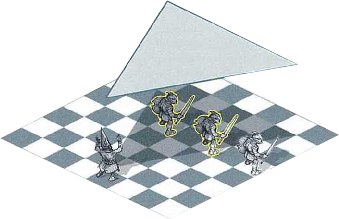
\includegraphics[scale=1]{img/ConoTemplate.png}
	\caption{Plantilla Conica}
	\label{img:plantillacono}
\end{figure}

\begin{figure}[hbtp]
	\centering
	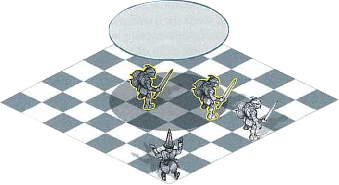
\includegraphics[scale=1]{img/CirculoTemplate.png}
	\caption{Plantilla Esferica}
	\label{img:plantillaesfera}
\end{figure}

\begin{figure}[hbtp]
	\centering
	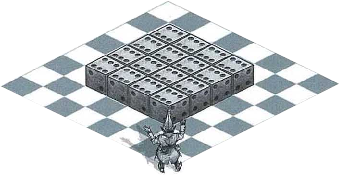
\includegraphics[scale=1]{img/CuadradoToken.png}
	\caption{Fichas Rectangular}
	\label{img:token_rec}
\end{figure}

\begin{figure}[hbtp]
	\centering
	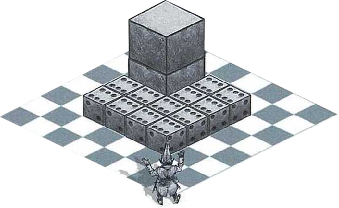
\includegraphics[scale=1]{img/CuadradoTotalToken.png}
	\caption{Fichas Rectangular con Cubierta Total}
	\label{img:token_rec_total}
\end{figure}
 
\begin{figure*}[htp]
	\centering
	\subfloat[]{%
		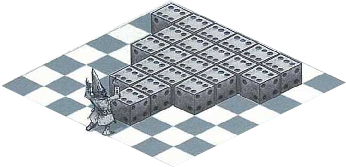
\includegraphics[scale=1]{img/conotokena.png}%
	}
	\subfloat[]{%
		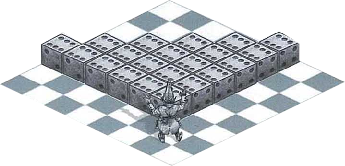
\includegraphics[scale=1]{img/conotokenbpng.png}%
	}
	\caption{Conos usando Fichas}
	\label{img:token_cono}
\end{figure*}

\begin{figure*}[htp]
	\centering
	\subfloat[]{%
		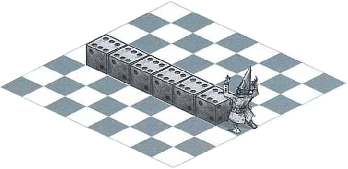
\includegraphics[scale=1]{img/linealtokena.png}%
	}
	\subfloat[]{%
		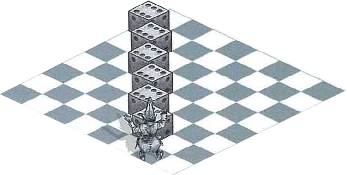
\includegraphics[scale=1]{img/linealtokenb.png}%
	}

	\subfloat[]{%
		\includegraphics[scale=1]{img/linealtokenc.png}%
	}
	\subfloat[]{%
		\includegraphics[scale=1]{img/linealtokend.png}%
	}
	\caption{Lineas usando Fichas}
	\label{img:token_linea}
\end{figure*}
 
\subsubsection{Metodo de las Fichas}
El método de las fichas está pensado para conseguir un efecto táctil y divertido. Para utilizar este método, coge unos dados u
otras fichas, que vas a utilizar para presentar tu efecto.

En lugar de representar fielmente las formas de las diferentes áreas de efecto, este método te da una forma de crear fácilmente
versiones de bordes cuadrados de ellas en una cuadrícula, como se describe en las siguientes subsecciones. 

\subparagraph{Usando Fichas} Cada cuadrado de 5 pies de un área de un defecto se convierte en un dado u otra ficha que se coloca
en la cuadrícula. Cada ficha va dentro de un cuadrado, no en una intersección de líneas. Si la ficha de un área está en un
cuadrado, ese cuadrado se incluye en el área de efecto. Es así de simple.

Las figuras \ref{img:token_rec}, \ref{img:token_rec_total}, \ref{img:token_cono} y \ref{img:token_linea} muestran este método en
acción, usando los dados como fichas. 

\subparagraph{Círculos} Este método representa todo usando cuadrados, y un área circular de efecto se convierte en cuadrada en
ella, ya sea que el área sea una esfera, un cilindro, o un radio. Por ejemplo, el radio de 10 pies de alcance de la llama, que
tiene un diámetro de 20 pies, se expresa como un cuadrado de 20 pies de lado, como se muestra en la figuras \ref{img:token_rec}.
La diagrama \ref{img:token_rec_total} muestra esa área con cobertura total en su interior.

\subparagraph{Conos} Un cono está representado por filas de fichas en la cuadrícula, que se extienden desde el punto de origen
del cono. En las filas, los cuadrados son contiguos uno al lado del otro o de esquina a esquina, como se muestra en la figur
\ref{img:token_cono}. Para determinar el número de filas que contiene un cono, divide su longitud por 5. Por ejemplo, un cono de
30 pies contiene seis filas.

Aquí está cómo crear las filas. Comenzando con un cuadrado adyacente al punto de origen del cono, coloca una ficha. El cuadrado
puede ser ortogonal o diagonalmente adyacente al punto de origen. En cada fila más allá de ese punto, coloque tantas fichas como
las que colocó en la fila anterior, más una ficha más. Coloque las fichas de esta fila de manera que sus cuadrados se encuentren
a un lado de un cuadrado de la fila anterior. Si el cono es ortogonalmente adyacente al punto de origen, tendrá una ficha más
para colocar en la fila; colóquela en un extremo u otro de la fila que acaba de crear (no tiene que elegir el lado elegido en la
figura \ref{img:token_cono}). Siga colocando fichas de esta manera hasta que haya creado todas las filas del cono.

\subparagraph{Líneas} Una línea puede extenderse desde su origen en forma ortogonal o diagonal, como se muestra en el diagrama
\ref{img:token_linea}. 

\section{Contruccion de Encuentros}
Esta sección introduce nuevas directrices sobre la construcción de encuentros de combate para una aventura. Son una alternativa a
las reglas en ''Crear encuentros'' en el capítulo 3 de la Guía del Maestro de Calabozo. Este enfoque utiliza las mismas
matemáticas que subyacen en las reglas presentadas en ese libro, pero hace algunos ajustes en la forma en que las matemáticas se
presentan para producir un sistema más flexible.

Este sistema de construcción de encuentros asume que, como DM, quieres tener un claro entendimiento de la amenaza que representa
un grupo de monstruos. Te será útil si quieres enfatizar el combate en tu aventura, si quieres asegurarte de que un enemigo no es
demasiado mortal para un grupo de personajes, y si quieres entender la relación entre el nivel de un personaje y la clasificación
de un monstruo.

Para construir un encuentro utilizando estas pautas se siguen una serie de pasos. 

\subsection*{Paso 1: Evaluar a los Personajes}
Para construir un encuentro con este sistema, primero hay que hacer un balance de los personajes del jugador. Este sistema
utiliza los niveles de los personajes para determinar los números y las clasificaciones de los desafíos de las criaturas con las
que te puedes enfrentar sin hacer un combate demasiado difícil o demasiado fácil. Aunque el nivel de los personajes es importante,
también debes tener en cuenta el máximo punto de golpe de cada personaje y los modificadores de salvación de lanzamiento, así
como cuánto daño pueden soportar los personajes más poderosos con un solo ataque. El nivel de personaje y la puntuación de los
desafíos son buenos para definir la dificultad de un encuentro, pero no cuentan toda la historia. Utilizarás estas estadísticas
adicionales de los personajes cuando selecciones monstruos para un encuentro en el paso 4. 

\subsection*{Paso 2: Elegir el Tamaño del Encuentro}
Determina si quieres crear una batalla que enfrente a una criatura con los personajes o si quieres usar varios monstruos. Si la
lucha es contra un solo oponente, tu mejor candidato para ese enemigo es una de las criaturas legendarias del juego, que están
diseñadas para cubrir esta necesidad. Si la batalla implica a varios monstruos, decide aproximadamente cuántas criaturas quieres
usar antes de continuar con el paso 3.

\subsection*{Paso 3: Determinar los numeros y la Puntuacion de Desafio}
El proceso de construcción de combates en los que sólo hay un monstruo legendario es sencillo. La tabla de clasificación de
desafíos de monstruos solitarios te muestra qué clasificación de desafíos (CR) utilizar para una criatura legendaria que se
enfrente a un grupo de cuatro a seis personajes, creando una batalla satisfactoria pero difícil. Por ejemplo, para un grupo de
cinco personajes de 9º nivel, una criatura legendaria CR 12 realiza un encuentro óptimo.

Para una batalla más peligrosa, empareja a los personajes con una criatura legendaria cuya puntuación de desafío sea 1 o 2 más
alta que la óptima. Para un combate más fácil, utiliza una criatura legendaria cuya puntuación de desafío sea 3 o más inferior a
la óptima. 

\header{CR Criatura Solitaria}
\begin{dndtable}[cccc]
			& \multicolumn{3}{c}{Tamaño del Grupo}	\\
	lvl		& 6 Pjs		& 5 Pjs		& 4 PJs			\\
	1ro  	&  2		&  2		&  1			\\
	2do  	&  4		&  3		&  2			\\
	3ro  	&  5		&  4		&  3			\\
	4to  	&  6		&  5		&  4			\\
	5tt  	&  9		&  8		&  7			\\
	6to  	& 10		&  9		&  8			\\
	7mo  	& 11		& 10		&  9			\\
	8vo  	& 12		& 11		& 10			\\
	9no  	& 13		& 12		& 11			\\
	10mo 	& 14		& 13		& 12			\\
	11avo	& 15		& 14		& 13			\\
	12avo	& 17		& 16		& 15			\\
	13avo	& 18		& 17		& 16			\\
	14avo	& 19		& 18		& 17			\\
	15avo	& 20		& 19		& 18			\\
	16avo	& 21		& 20		& 19			\\
	17avo	& 22		& 21		& 20			\\
	18avo	& 22		& 21		& 20			\\
	19avo	& 23		& 22		& 21			\\
	20avo	& 24		& 23		& 22			\\
\end{dndtable}

Si tu encuentro presenta varios monstruos, equilibrarlo requiere un poco más de trabajo. Consulta las tablas de monstruos
múltiples, que están divididas por rangos de niveles, y proporcionan información sobre cómo equilibrar los encuentros de los
personajes de los niveles 1-5, 6-10, 11-15 y 16-20.

En primer lugar, es necesario anotar la clasificación de desafío para cada criatura que el grupo enfrente. Luego, para crear su
encuentro, encuentre el nivel de cada personaje en la tabla apropiada. Cada tabla muestra a qué equivale un solo personaje de un
nivel determinado en términos de puntuación de desafío, un valor representado por una proporción que compara el número de
personajes con un solo monstruo clasificado según la puntuación de desafío. El primer número de cada expresión es el número de
caracteres del nivel correspondiente. El segundo número indica a cuántos monstruos de la lista de clasificación de desafíos
equivalen esos personajes. 

Por ejemplo, leyendo la fila de personajes de 1er nivel de la tabla de 1er a 5to nivel, vemos que un personaje de 1er nivel es el
equivalente a dos monstruos CR 1/8 o un monstruo CR 1/4. La proporción se invierte para las clasificaciones de desafío más altas,
donde un solo monstruo es más poderoso que un solo personaje de 1er nivel. Una criatura CR 1/ 2 es equivalente a tres personajes
de 1er nivel, mientras que un oponente CR 1 es equivalente a cinco. 

Digamos que tienes un grupo de cuatro personajes de tercer nivel. Usando la tabla, puede ver que un enemigo CR 2 es un buen
partido para todo el grupo, pero que los personajes probablemente tendrán dificultades para manejar una criatura CR 3.

Usando las mismas pautas, puedes mezclar y hacer coincidir las clasificaciones de los desafíos para formar un grupo de criaturas
que se oponga a cuatro personajes de tercer nivel. Por ejemplo, podría seleccionar una criatura CR 1. Eso vale dos personajes de
tercer nivel, lo que te deja con el valor de dos personajes de monstruos para asignar. Luego podría agregar dos monstruos CR 1/4
para tener en cuenta otro personaje y un monstruo CR 1/2 para tener en cuenta el último personaje. En total, tu encuentro tiene
un CR 1, un CR 1/2 y dos CR 1/4. 

Para los grupos en los que los personajes son de diferentes niveles, tienes dos opciones. Puedes agrupar a todos los personajes
del mismo nivel, emparejarlos con monstruos y luego combinar todas las criaturas en un solo encuentro. Alternativamente, puedes
determinar el nivel medio del grupo y tratar a cada personaje como si fuera de ese nivel con el propósito de seleccionar los
monstruos apropiados.

Las pautas anteriores están diseñadas para crear una pelea que desafíe a un grupo y que al mismo tiempo sea ganable. Si quieres
crear un encuentro más fácil que desafíe a los personajes pero que no amenace con derrotarlos, puedes tratar al grupo como si
fuera aproximadamente un tercio más pequeño de lo que es. Por ejemplo, para crear un encuentro fácil para un grupo de cinco
personajes, enfréntalos a monstruos que serían una dura lucha para tres personajes. De igual modo, puedes tratar al grupo como si
fuera un poco más grande para construir una batalla potencialmente mortal, aunque no es probable que sea una derrota automática.
Un grupo de cuatro personajes que se enfrente a un encuentro diseñado para seis personajes entraría en esta categoría. 

\subsubsection*{Monstruos Debiles y Personajes Fuertes}

Para ahorrar espacio en las tablas y mantenerlas sencillas, algunas de las clasificaciones de desafío más bajas no se encuentran
en las tablas de nivel superior. Para las clasificaciones de desafíos bajas que no aparecen en la tabla, supongamos una relación
de 1:12, lo que indica que doce criaturas de esas clasificaciones de desafíos equivalen a un personaje de un nivel específico. 

\begin{table*}[hp]%
	\begin{dndtable}[cccccccccc]
		\multicolumn{10}{c}{\textbf{Multiples Criaturas: Niveles 1ro al 5to}}		\\
		\textbf{lvl} & \textbf{1/8} & \textbf{1/4} & \textbf{1/2} & \textbf{1} & \textbf{2} & \textbf{3} & \textbf{4} & \textbf{5} & \textbf{6}	\\
		1ro			 & 1:2 			& 1:1		   & 3:1		  & 5:1		   & -			& -			 & -		& -			   & -			\\
		2do			 & 1:3 			& 1:2		   & 1:1		  & 3:1		   & 6:1		& -			 & -		& -			   & -			\\
		3ro			 & 1:5 			& 1:2		   & 1:1		  & 2:1		   & 4:1		& 6:1		 & -		& -			   & -			\\
		4to			 & 1:8 			& 1:4		   & 1:2		  & 1:1		   & 2:1		& 4:1		 & 6:1		& -			   & -			\\
		5to			 & 1:12			& 1:8		   & 1:4		  & 1:2		   & 1:1		& 2:1		 & 3:1		& 5:1		   & 6:1		\\
	\end{dndtable}
\end{table*}

\begin{table*}[hp]%
	\begin{dndtable}[cccccccccccccc]
		\multicolumn{14}{c}{\textbf{Multiples Criaturas: Niveles 6to al 10mo}}		\\
		\textbf{lvl} & \textbf{1/8} & \textbf{1/4} & \textbf{1/2} & \textbf{1} & \textbf{2} & \textbf{3} & \textbf{4} & \textbf{5} & \textbf{6} & \textbf{7} & \textbf{8} & \textbf{9} & \textbf{10} 	\\
		6to			 & 1:12 		& 1:9		   & 1:5		  & 1:2		   & 1:1		& 2:1		 & 2:1		  & 4:1		   & 5:1		& 6:1		 & -		  & -		   & -				\\
		7mo			 & 1:12 		& 1:12		   & 1:6		  & 1:3		   & 1:1		& 1:1		 & 2:1		  & 3:1		   & 4:1		& 5:1		 & -		  & -		   & -				\\
		8vo			 & 1:12 		& 1:12		   & 1:7		  & 1:4		   & 1:2		& 1:1		 & 2:1		  & 3:1		   & 3:1		& 4:1		 & 6:1		  & -		   & -				\\
		9no			 & 1:12 		& 1:12		   & 1:8		  & 1:4		   & 1:2		& 1:1		 & 1:1		  & 2:1		   & 3:1		& 4:1		 & 5:1		  & 6:1		   & -				\\
		10mo		 & 1:12			& 1:12		   & 1:10		  & 1:5		   & 1:2		& 1:1		 & 1:1		  & 2:1		   & 2:1		& 3:1		 & 4:1		  & 5:1		   & 6:1			\\
	\end{dndtable}
\end{table*}

\begin{table*}[hp]%
	\begin{dndtable}[cccccccccccccccc]
		\multicolumn{16}{c}{\textbf{Multiples Criaturas: Niveles 11avo al 15avo}}		\\
		\textbf{lvl} & \textbf{1}   & \textbf{2}   & \textbf{3}   & \textbf{4} & \textbf{5} & \textbf{6} & \textbf{7} & \textbf{8} & \textbf{9} & \textbf{10}& \textbf{11}& \textbf{12}& \textbf{13} & \textbf{14} & \textbf{15}	\\
		11avo		 & 1:6 			& 1:3		   & 1:2		  & 1:1		   & 2:1		& 2:1		 & 2:1		  & 3:1		   & 4:1		& 5:1		 & 6:1		  & -		   & - 			 & - 		   & - 		\\
		12avo		 & 1:8 			& 1:3		   & 1:2		  & 1:1		   & 1:1		& 2:1		 & 2:1		  & 3:1		   & 3:1		& 4:1		 & 5:1		  & 6:1		   & - 			 & - 		   & - 		\\
		13avo		 & 1:9 			& 1:4		   & 1:2		  & 1:2		   & 1:1		& 1:1		 & 2:1		  & 2:1		   & 3:1		& 3:1		 & 4:1		  & 5:1		   & 6:1		 & -		   & -		\\
		14avo		 & 1:10 		& 1:4		   & 1:3		  & 1:2		   & 1:1		& 1:1		 & 2:1		  & 2:1		   & 3:1		& 3:1		 & 4:1		  & 4:1		   & 5:1		 & 6:1		   & -		\\
		15avo		 & 1:12			& 1:5		   & 1:3		  & 1:2		   & 1:1		& 1:1		 & 1:1		  & 2:1		   & 2:1		& 3:1		 & 3:1		  & 4:1		   & 5:1		 & 5:1		   & 6:1	\\
	\end{dndtable}
\end{table*}

\begin{table*}[hp]%
	\begin{dndtable}[cccccccccccccccccccc]
		\multicolumn{20}{c}{\textbf{Multiples Criaturas: Niveles 16avo al 20avo}}		\\
		\textbf{lvl} & \textbf{2}   & \textbf{3}   & \textbf{4} & \textbf{5} & \textbf{6} & \textbf{7} & \textbf{8} & \textbf{9} & \textbf{10}& \textbf{11}& \textbf{12}& \textbf{13} & \textbf{14} & \textbf{15} & \textbf{16} & \textbf{17} & \textbf{18} & \textbf{19} & \textbf{20}	\\
		16avo		 & 1:5 			& 1:3		   & 1:2		& 1:1		 & 1:1		  & 1:1		   & 2:1		& 2:1		 & 2:1		  & 3:1		   & 4:1		& 4:1		  & 5:1			& 5:1		  & 6:1			& - 		  & -			& -			  & -			\\
		17avo		 & 1:7 			& 1:4		   & 1:3		& 1:2		 & 1:1		  & 1:1		   & 1:1		& 2:1		 & 2:1		  & 2:1		   & 3:1		& 3:1		  & 4:1			& 4:1		  & 5:1			& 6:1 		  & -			& -			  & -			\\
		18avo		 & 1:7 			& 1:5		   & 1:3		& 1:2		 & 1:1		  & 1:1		   & 1:1		& 2:1		 & 2:1		  & 2:1		   & 3:1		& 3:1		  & 4:1			& 4:1		  & 5:1			& 6:1		  & 6:1			& -			  & -			\\
		19avo		 & 1:8 			& 1:5		   & 1:3		& 1:2		 & 1:2		  & 1:1		   & 1:1		& 1:1		 & 2:1		  & 2:1		   & 2:1		& 3:1		  & 3:1			& 4:1		  & 4:1			& 5:1		  & 6:1			& 6:1		  & -			\\
		20avo		 & 1:9			& 1:6		   & 1:4		& 1:2		 & 1:2		  & 1:1		   & 1:1		& 1:1		 & 1:1		  & 2:1		   & 2:1		& 2:1		  & 3:1			& 3:1		  & 4:1			& 4:1		  & 5:1			& 5:1		  & 6:1			\\
	\end{dndtable}
\end{table*}

\subsection*{Paso 4: Seleccionar los Monstruos}
Después de utilizar las tablas del paso anterior para determinar las clasificaciones de desafío de los monstruos de tu encuentro,
estás listo para elegir monstruos individuales. Este proceso es más bien un arte que una ciencia.

Además de evaluar a los monstruos según la clasificación de desafío, es importante ver cómo ciertos monstruos pueden compararse
con tu grupo. Los puntos de golpe, los ataques y los tiros de salvación son todos indicadores útiles. Compara el daño que un
monstruo puede causar con el máximo de puntos de golpe de cada personaje. Ten cuidado con cualquier monstruo que sea capaz de
derribar a un personaje con un solo ataque, a menos que estés diseñando la lucha para que sea especialmente mortal.

De la misma manera, compara los puntos de golpe de los monstruos con el daño producido por los personajes más fuertes del grupo,
buscando de nuevo objetivos que puedan ser matados con un solo golpe. Si un número significativo de enemigos cae en las primeras
rondas de combate, el encuentro puede resultar demasiado fácil.

Del mismo modo, mira si las habilidades más mortíferas de un monstruo requieren lanzamientos de salvación con los que la mayoría
de los miembros del grupo son débiles, y compara las habilidades ofensivas de los personajes con los lanzamientos de salvación de
los monstruos.

Si las únicas criaturas que puedes elegir con la puntuación de desafío deseada no se ajustan bien a las estadísticas de los
personajes, no tengas miedo de volver al paso 3. Al cambiar los objetivos de la puntuación de desafío y ajustar el número de
criaturas en el encuentro, puedes crear diferentes opciones para construir el encuentro. 

\subsection*{Paso 5: Añadir Sabor}
Los eventos que se desarrollan durante un encou nter tienen que ver con mucho más que el balanceo de las armas y el lanzamiento
de conjuros. Los enfrentamientos más interesantes también tienen en cuenta la personalidad o el comportamiento de los monstruos,
quizás determinando si se pueden comunicar con ellos o si todos están actuando en conjunto. Otros factores posibles incluyen la
naturaleza del entorno físico, como si incluye obstáculos u otras características que puedan entrar en juego, y la posibilidad
siempre presente de que ocurra algo inesperado.

Si ya tienes ideas de cómo dar cuerpo a tu encuentro de esta manera, ve directo al grano y termina tu creación. De lo contrario,
echa un vistazo a las siguientes secciones para obtener algunos consejos básicos sobre cómo añadir elementos de sabor a la
sencilla mecánica de la lucha. 

\subsubsection*{Personalidad del Monstruo}
Para abordar la cuestión de la personalidad de un monstruo, puedes utilizar las tablas del capítulo 4 de la Guía del Maestro de
la Mazmorra, utilizar la tabla de Personalidad de Monstruo que aparece a continuación o simplemente anotar algunas notas basadas
en la descripción del Manual de Monstruos de una criatura. Durante la batalla, puedes usar estas ideas para informar de cómo
retratas a los monstruos y sus acciones. Para simplificar, puedes asignar los mismos rasgos de personalidad a un grupo entero de
monstruos. Por ejemplo, una banda de bandidos puede ser una banda rebelde de fanfarrones, mientras que los miembros de otra banda
están siempre al límite y listos para huir a la primera señal de peligro. 

\begin{dndtable}[cX]
	\textbf{d8}	& \textbf{Personalidad}	\\
	1			& Cobarde; buscando rendirse	\\
	2			& Codicioso; quiere el tesoro	\\
	3			& Fanfarrón; hace una muestra de valentía pero huye del peligro	\\
	4			& Fanático; listo para morir luchando	\\
	5			& Chusma; mal entrenada y fácilmente agitada	\\
	6			& Valiente; se mantiene firme	\\
	7			& bromista; se burla de sus enemigos	\\
	8			& Acosador; se niega a creer que puede perder	\\
\end{dndtable}

\subsubsection*{Relaciones de Monstruos}
¿Existen rivalidades, odios o apegos entre los monstruos en un encuentro? Si es así, puedes usar tales relaciones para informar
el comportamiento de los monstruos durante el combate. La muerte de un líder muy reverenciado puede poner a sus seguidores en un
frenesí. Por otro lado, un monstruo puede decidir huir si su cónyuge muere, o un sapo maltratado puede estar ansioso por rendirse
y traicionar a su amo a cambio de su vida. 

\begin{dndtable}[cX]
	\textbf{d6}	& \textbf{Relaciones}	\\
	1			& Tiene un rival; quiere que un aliado al azar sufra	\\
	2			& Es abusado por otros; se queda atrás, traiciona a la primera oportunidad	\\
	3			& Es adorado; los aliados morirán por ello	\\
	4			& Es rechazado por el grupo; es un lazo que lo ignora.	\\
	5			& Es rechazado por elección; sólo se preocupa por sí mismo	\\
	6			& Es visto como un matón; sus aliados no querían verlo derrotado 	\\
\end{dndtable}

\subsubsection*{Terreno y Trampas}
Unos pocos elementos que hacen que un campo de batalla sea algo más que una gran área de terreno plano pueden contribuir en gran
medida a condimentar un encuentro. Considere la posibilidad de establecer su encuentro en un área que le proporcione desafíos, 
incluso si no se está llevando a cabo una pelea allí. ¿Qué peligros potenciales u otras características podrían llamar la
atención de los personajes, ya sea antes o durante la pelea? ¿Por qué son los monstruos los que acechan en esta área para empezar?

Para añadir detalles a un área de un encuentro al azar, mira a las tablas en el apéndice A de la Guía del Maestro de la Mazmorra
para determinar las características del cuarto y del área, los peligros potenciales, los obstáculos, las trampas y más. 

\subsubsection*{Eventos Aleatorios}
Considere lo que podría ocurrir en un encuentro si los personajes no llegasen a entrar en él. ¿Los guardias sirven por períodos
de tiempo? ¿Qué otros personajes o monstruos podrían visitar? ¿Se reúnen allí las criaturas para comer o chismorrear? ¿Hay algún
fenómeno natural -como fuertes vientos, temblores de tierra o lluvia- que a veces ocurre en el área? Los eventos aleatorios
pueden añadir un elemento divertido de lo inesperado a un n encuentro. Justo cuando crees que el resultado de una pelea es
evidente, un evento imprevisto puede hacer las cosas más convincentes.

Varias de las tablas de la Guía del Maestro de la Mazmorra pueden sugerir eventos aleatorios. Las tablas utilizadas para la
localización del encuentro, los lugares extraños y el tiempo salvaje en el capítulo 5 de ese libro son un buen punto de partida
para los encuentros al aire libre. Las tablas en el apéndice A pueden ser útiles para encuentros interiores y exteriores -
especialmente las tablas para obstáculos, trampas, y trucos. Finalmente, consulta las tablas de encuentros al azar en la
siguiente sección de este libro para inspirarte. 

\subsection{Emparejamientos Rapudos}
Las pautas anteriores asumen que ustedes están preocupados por el equilibrio en sus encuentros de combate y tienen suficiente
tiempo para prepararlos. Si no dispone de mucho tiempo, o si desea unas pautas más sencillas pero menos precisas, la tabla de
Parejas Rápidas que aparece a continuación ofrece una alternativa.

Esta tabla te da una forma de emparejar un personaje de un cierto nivel con un número de monstruos. En la tabla se indican las
clasificaciones de los desafíos que se deben utilizar para incluir uno, dos y cuatro monstruos por personaje en cada nivel. Por
ejemplo, al mirar la entrada de tercer nivel de la tabla, puedes ver que un monstruo CR 1/2 equivale a un personaje de tercer
nivel, al igual que dos monstruos CR 1/4 y cuatro CR 1/8. 

\begin{dndtable}[cccc]
	\textbf{nivel}		& \textbf{1 Enemigo}	& \textbf{1 Enemigo}	& \textbf{1 Enemigo}		\\
	1st 		& 1/4		& 1/8		& -  			\\
	2nd 		& 1/2		& 1/4		& -  			\\
	3rd 		& 1/2		& 1/4		& 1/8			\\
	4th 		& 1  		& 1/2		& 1/4			\\
	5th 		& 2  		& 1  		& 1/2			\\
	6th 		& 2  		& 1  		& 1/2			\\
	7th 		& 3  		& 1  		& 1/2			\\
	8th 		& 3  		& 2  		& 1  			\\
	9th 		& 4  		& 2  		& 1  			\\
	10th		& 4  		& 2  		& 1  			\\
	11th		& 4  		& 3  		& 2  			\\
	12th		& 5  		& 3  		& 2  			\\
	13th		& 6  		& 4  		& 2  			\\
	14th		& 6  		& 4  		& 2  			\\
	15th		& 7  		& 4  		& 3  			\\
	16th		& 7  		& 4  		& 3  			\\
	17th		& 8  		& 5  		& 3  			\\
	18th		& 8  		& 5  		& 3  			\\
	19th		& 9  		& 6  		& 4  			\\
	20th		& 10 		& 6  		& 4  			\\
\end{dndtable}

\section{Encuentros Aleatorios: Un mundo de Posibilidades}
El capítulo 3 de la Guía del Maestro de Calabozo proporciona la guía para usar encuentros al azar en tu juego. Esta sección se
basa en esa guía, ofreciendo una serie de tablas de encuentros aleatorios para que usted utilice cuando determine que un
encuentro aleatorio va a tener lugar.

Utilizando como base las listas de monstruos del apéndice B de ese libro, hemos construido un conjunto de tablas para cada
categoría de entorno: ártico, costa, desierto, bosque, pradera, colina, montaña, pantano, subsuelo, y urbano. Dentro de cada
categoría, se proporcionan tablas de clasificación para cada uno de los cuatro niveles de juego: niveles 1- 4, 5- 10, 11- 16, y
17-20.

Aunque usted puede utilizar estas tablas ''fuera de la caja,'' el consejo en la Guía del Maestro de Calabozo todavía es verdad: la
adaptación de tales tablas a su ga me puede informar los temas y el sabor de su campaña. Le animamos a personalizar este material
para hacerlo suyo.

En las tablas, un nombre en negrita hace referencia a un bloque de estadísticas del Manual de monstruos. 

\subsection*{Vuela, o Lucha, o ...?}
Cada uno de los resultados de estas tablas representa un cierto tipo de desafío o reto potencial.

Si dejas que los dados se salgan con la suya y el resultado es un gran número de monstruos, el encuentro generado puede ser
demasiado difícil o peligroso para los personajes en sus actuales circunstancias. Es posible que quieran huir para evitar el
contacto, o no acercarse más después de percibir los monstruos a distancia.

Por supuesto, también tienes la libertad de ajustar los números, pero es importante recordar que no todos los encuentros con un
monstruo tienen que resultar en un combate. Un encuentro puede ser, en efecto, el preludio de una batalla, un parlamento o alguna
otra interacción. Lo que sucede a continuación depende de lo que intenten los personajes, o lo que decidas que va a ocurrir.

Las tablas también incluyen entradas para lo que la Guía del Maestro de Calabozo llama ''encuentros de naturaleza menos
monstruosa''. Muchos de estos resultados piden a gritos ser personalizados o detallados, lo que te ofrece la oportunidad de
conectarlos con la historia de tu campaña. Y al hacerlo, has dado un paso más hacia tu propia mesa de encuentros. Ahora, ¡siga
adelante! 

\newpage
\subsection{Encuentros en el Artico}

\begin{dndtable}[cX]
	\multicolumn{2}{c}{\textbf{Artico: Nvl 1-4}}		\\
	\textbf{d100}	& \textbf{Encuentro}	\\
	1				& 1 búho gigante	\\
	2 - 5			& 1d6 + 3 kobolds	\\
	6 - 8			& 1d4 + 3 tramperos (plebeyos)	\\
	9 - 10			& 1 búho	\\
	11 - 12			& 2d4 halcones de sangre	\\
	13 - 17			& 2d6 bandidos	\\
	18 - 20			& 1d3 Kobolds alados con 1d6 kobolds	\\
	21 - 25			& El cadáver parcialmente comido de un mamut, del cual se pueden cosechar 1d4 semanas de raciones	\\
	26 - 29			& 2d8 cazadores (guerreros tribales)	\\
	30 - 35			& 1 Semiogro	\\
	36 - 40			& Las pistas de una sola fila en la nieve se detienen abruptamente	\\
	41 - 45			& 1d3 mefistófonos de hielo	\\
	46 - 50			& 1 oso pardo	\\
	51 - 53			& 1d6 + 1 orcos	\\
	54 - 55			& 1 oso polar	\\
	56 - 57			& 1d6 exploradores	\\
	58 - 60			& 1 tigre de dientes de sable	\\
	61 - 65			& Un estanque congelado con un agujero dentado en el hielo que parece hecho recientemente	\\
	66 - 68			& 1 berserker	\\
	69 - 70			& 1 ogro	\\
	71 - 72			& 1 grifón	\\
	73 - 75			& 1 druida	\\
	76 - 80			& 3d4 refugiados (plebeyos) que huyen de los minerales 	\\
	81				& 1d3 veteranos	\\
	82				& 1d4 orogs	\\
	82				& 2 osos pardos	\\
	84				& 1 orco Ojo de Gruumsh con 2d8 orco	\\
	85				& 1d3 lobos de invierno	\\
	86 - 87			& 1d4 yetis	\\
	88				& 1 Semiogro	\\
	89				& 1d3 manticoras	\\
	90				& 1 capitán de bandido con 2d6 bandidos	\\
	91				& 1 vengador	\\
	92 - 93			& 1 trol	\\
	94 - 95			& 1 Hombre-oso	\\
	96 - 97			& 1 joven remorhaz	\\
	98				& 1 mamut	\\
	99				& 1 joven dragón blanco	\\
	00				& 1 gigante de hielo 	\\
\end{dndtable}

\begin{dndtable}[cX]
	\multicolumn{2}{c}{\textbf{Artico: Nvl 5-10}}		\\
	\textbf{d100}	& \textbf{Encuentro}	\\
	1 - 5			& 2 tigres de dientes de sable	\\
	6 - 7			& 1d4 Semiogro	\\
	8 - 10			& 1d3 + 1 osos pardos	\\
	11 - 15			& 1d3 osos polares	\\
	16 - 20			& 2d4 berserkers	\\
	21 - 25			& Un druida medio muerto atendiendo a un oso polar herido. Si los personajes asisten al druida, ella les da un frasco de antitoxina.	\\
	26 - 30			& 2d8 exploradores	\\
	31 - 35			& 2d4 méphits de hielos	\\
	36 - 40			& 2d6 + 1 zombies a bordo de un galeón atrapados en el hielo. La búsqueda en el barco produce 2d20 días de raciones.	\\
	41 - 45			& 1 manticora	\\
	46 - 50			& 2d6 + 3 orcos	\\
	51 - 53			& 1d6 + 2 ogros	\\
	54 - 55			& 2d4 grifos	\\
	56 - 57			& 1d4 veteranos	\\
	58 - 60			& 1 capitán bandido con 1 druida, 1d3 berserkers, y 2d10 + 5 bandidos	\\
	61 - 65			& 1d4 horas de frío extremo (véase el capítulo 5 de la Guía del Maestro de Calabozo)	\\
	66 - 68			& 1 joven remorhaz	\\
	69 - 72			& 1 orco Ojo de Gruumsh con 1d6 orogs y 2d8 + 6 orcos	\\
	73 - 75			& 1 vengador	\\
	76 - 80			& Un aullido que resuena sobre la tierra durante 3 minutos.	\\
	81 - 82			& 1d3 mamuts	\\
	83 - 84			& 1 joven dragón blanco	\\
	85 - 86			& 2d4 lobos de invierno	\\
	87 - 88			& 1d6 + 2 yetis	\\
	89 - 90			& 1d2 gigantes de hielo	\\
	91 - 92			& 1d3 werebears	\\
	93 - 94			& 1d4 trolls	\\
	95 - 96			& 1 abominable yeti	\\
	97 - 98			& 1 remorhaz	\\
	99				& 1 hueva	\\
	00				& 2d4 jóvenes remorhazes 	\\
\end{dndtable}

\begin{dndtable}[cX]
	\multicolumn{2}{c}{\textbf{Artico: Nvl 11-16}}		\\
	\textbf{d100}	& \textbf{Encuentro}	\\
	1				& 1 abominable yeti	\\
	2 - 4			& 1d6 vengadores	\\
	5 - 10			& 1d4 + 1 hombre-oso	\\
	11 - 20			& 1d3 jóvenes dragones blancos	\\
	21 - 25			& Una ventisca que reduce la visibilidad a 5 pies durante 1d6 horas	\\
	26 - 35			& 1 roc	\\
\end{dndtable}

\begin{dndtable}[cX]
	\textbf{d100}	& \textbf{Encuentro}	\\
	36 - 40			& Una manada de 3d20 + 60 caribúes (ciervos) moviéndose por la nieve	\\
	41 - 50			& 1d4 mamuts	\\
	51 - 60			& 1d8 + 1 trolls	\\
	61 - 65			& Un lago congelado de una milla de ancho en el que se pueden ver los cadáveres conservados de extrañas criaturas.	\\
	66 - 75			& 2d4 jóvenes remorhazes	\\
	76 - 80			& Un castillo de hielo en ruinas lleno de cuerpos congelados de humanoides de piel azul...	\\
	81 - 90			& 1 dragón blanco adulto	\\
	91 - 96			& 1d8 + 1 gigante de hielo	\\
	97 - 99			& 1d4 remorhazes	\\
	00				& 1 dragón blanco antiguo 	\\
\end{dndtable}

\begin{dndtable}[cX]
	\multicolumn{2}{c}{\textbf{Artico: Nvl 17-20}}		\\
	\textbf{d100}	& \textbf{Encuentro}	\\
	 1 -  2			& 2d10 revenants	\\
	 3 -  4			& 2d8 Trolls	\\
	 5 -  6			& 2d10 ositos de peluche	\\
	 7 -  8			& 1 gigante de hielo	\\
	 9 - 10			& 2d4 jóvenes remorhazes	\\
	11 - 20			& 1d4 gigantes de hielo	\\
	21 - 25			& Un parche circular de hielo negro en el suelo. La temperatura del aire alrededor del parche es más cálida que en el área circundante, y los personajes que inspeccionan el hielo encuentran trozos de maquinaria congelados en su interior.	\\
	26 - 35			& 1 antiguo dragón blanco	\\
	36 - 40			& Un aventurero congelado a 6 pies bajo el hielo; 50\% de probabilidad de que el cadáver tenga un raro objeto mágico de la elección del DM	\\
	41 - 50			& 1d3 abominables yetis	\\
	51 - 60			& 1d4 remorhazes	\\
	61 - 65			& Una pared de hielo de 500 pies de altura que tiene 300 pies de espesor a lo largo de 1d4 millas	\\
	66 - 75			& 1d4 rocs	\\
	76 - 80			& La imagen de una mujer severa con pelo largo y suelto, esculpido en la ladera de una montaña	\\
	81 - 90			& 1d10 gigantes de hielo con osos polares de 2d4	\\
	91 - 96			& 1d3 dragones blancos adultos	\\
	00     			& 2d4 abominables yetis	\\
\end{dndtable}

%\newpage
\subsection{Encuentros en la Costa}
\begin{dndtable}[cX]
	\multicolumn{2}{c}{\textbf{Costa: Nvl 1-4}}		\\
	\textbf{d100}	& \textbf{Encuentro}	\\
	01				& 1 pseudodragón	\\
	02 - 05			& 2d8 cangrejos	\\
	06 - 10			& 2d6 pescadores (plebeyos)	\\
	11				& 1d3 serpientes venenosas	\\
	12 - 13			& 1d6 guardias protegiendo a un noble varado	\\
	14 - 15			& 2d4 scouts	\\
	16 - 18			& 2d10 merfolk	\\
	19 - 20			& 1d6 + 2 sahuagin	\\
	21 - 25			& 1d4 ghouls alimentándose de cadáveres a bordo de los restos de un barco mercante. Una búsqueda descubre 2d6 pernos de seda en ruinas, una cuerda de 5O pies de largo y un barril de arenque salado.	\\
	26 - 27			& 1d4 kobolds alados con ld6 + 1 kobolds	\\
	28 - 29			& 2d6 guerreros tribales	\\
	30 - 31			& 3d4 kobolds	\\
	32 - 33			& 2d4 + 5 halcones de sangre	\\
	34 - 35			& 1d8 + 1 pteranodones	\\
	36 - 40			& Unas pocas docenas de tortugas bebé luchando por abrirse camino en el mar	\\
	41 - 42			& 1d6 + 2 lagartos gigantes	\\
	43 - 44			& 1d6 + 4 cangrejos gigantes	\\
	45 - 46			& 2d4 stirges	\\
	47 - 48			& 2d6 + 3 bandidos	\\
	49 - 53			& 2d4 sahuagin	\\
	54 - 55			& 1d6 + 2 scouts	\\
	56 - 60			& 1 bruja del mar	\\
	61 - 65			& Una formación momentánea en las ondas que parece un enorme rostro humanoide	\\
	66 - 70			& 1 druida	\\
	71 - 75			& 1d4 arpías	\\
	76 - 80			& Un ermitaño solitario (acólito) sentado en la playa, contemplando el significado del multiverso	\\
	81				& 1d4 berserkers	\\
	82				& 1d6 águilas gigantes	\\
	83				& 2d4 sapos gigantes	\\
	84				& 1d4 ogros o 1d4 merrow	\\
	85				& 3d6 sahuagin	\\
	86				& 1d4 veteranos	\\
	87				& 1d2 plesiosaurios	\\
	88				& 1 capitán de bandido con 2d6 bandidos	\\
	89				& 1d3 manticulas	\\
	90				& 1 banshee	\\
	91 - 92			& 1d4 + 3 grifos	\\
	93 - 94			& 1 sacerdotisa sahuagin con 1d3 merrow y 2d6 sahuagin	\\
	95 - 96			& 1 barón sahuagín	\\
\end{dndtable}

\begin{dndtable}[cX]
	\textbf{d100}	& \textbf{Encuentro}	\\
	97 - 98			& 1 elemental de agua	\\
	99				& 1 cíclope	\\
	00				& 1 joven dragón de bronce 	\\
\end{dndtable}

\begin{dndtable}[cX]
	\multicolumn{2}{c}{\textbf{Costa: Nvl 5-10}}		\\
	\textbf{d100}	& \textbf{Encuentro}	\\
	1				& 2d8 araña lobo gigante	\\
	2 - 3			& pteranodones 3d6	\\
	4 - 5			& 2d4 scouts	\\
	6 - 7			& 1d6 + 2 sahuagin	\\
	8				& 1 bruja del mar	\\
	9 - 10			& 1d4 + 1 sapo gigante	\\
	11 - 15			& 3d6 sahuagin	\\
	16 - 20			& 2d6 águilas gigantes	\\
	21 - 25			& Un pseudodragón persiguiendo gaviotas por el aire	\\
	26 - 29			& 1d2 druidas	\\
	30 - 32			& 2d4 + 1 sapo gigante	\\
	33 - 35			& 1 plebeyo cantando un canto de canto (sólo día) o 1 banshee (sólo noche)	\\
	36 - 40			& Una botella tapada que contiene un billete ilegible y medio enterrado en la arena	\\
	41 - 43			& 3 brujas del mar	\\
	44 - 46			& 1d8 + l arpías	\\
	47 - 50			& 1d4 plesiosaurios	\\
	51 - 53			& 1d4 manticulas	\\
	54 - 56			& 2d4 ogros	\\
	57 - 60			& Grifos de 1d1O	\\
	61 - 65			& Una batalla en el mar entre dos galeones	\\
	66 - 70			& 1d4 + 3 merrow	\\
	71 - 75			& Una tripulación pirata compuesta por un capitán bandido, un druida, dos berserkers y 2d12 bandidos, todos buscando para el tesoro enterrado	\\
	76 - 80			& Una mano humanoide cortada y enredada en una red	\\
	81 - 82			& 1 elemental de agua	\\
	83 - 84			& 1 cíclope	\\
	85 - 86			& 1d4 banshees (noche solamente)	\\
	87 - 88			& 2d4 veteranos	\\
	89 - 90			& 1 joven dragón de bronce	\\
	91 - 93			& 1d3 cíclopes	\\
	94 - 95			& 1 joven dragón azul	\\
	96				& 1 barón sahuagin con sacerdotisas sahuagin de 1d3 y sahuagin de 2d8	\\
	97				& 1 djinni	\\
	98				& 1 roc	\\
	99				& 1 maridaje	\\
	00				& 1 gigante de la tormenta 	\\
\end{dndtable}

\begin{dndtable}[cX]
	\multicolumn{2}{c}{\textbf{Costa: Nvl 11-16}}		\\
	\textbf{d100}	& \textbf{Encuentro}	\\
	1				& 1d4 banshees (sólo de noche)	\\
	2 - 4			& 1 cíclope	\\
	5 - 8			& 1d6 + 2 manticoras	\\
	9 - 10			& 1d8 + 2 veteranos	\\
	11 - 20			& 1 joven dragón azul	\\
	21 - 25			& Un nido de 1d6 huevos de tortuga dragón	\\
	26 - 35			& 1d4 barones sahuagineses	\\
	36 - 40			& Un tridente parcialmente enterrado en la arena	\\
	41 - 50			& 1 joven dragón de bronce	\\
	51 - 55			& 1 maridaje	\\
	56 - 60			& 1d6 elementos de agua	\\
	61 - 65			& 2d6 ghasts arrastrándose sobre los barcos naufragados de 1d6 y alimentándose de los muertos	\\
	66 - 70			& 1 djinni	\\
	71 - 75			& 1d3 jóvenes dragones de bronce	\\
	76 - 80			& Una ballena encallada, muerta e hinchada. Si recibe algún daño, explota, y cada criatura a menos de 30 pies de ella debe hacer un lanzamiento de salvamento de DC 15 Dexterity, recibiendo 5d6 de daño por apaleamiento en un salvamento fallido, o la mitad de daño en uno exitoso.	\\
	81 - 82			& 2d4 cíclopes	\\
	83 - 84			& 1 gigante de la tormenta	\\
	85 - 86			& 1d3 jóvenes dragones azules 	\\
	87 - 88			& 1 dragón de bronce adulto	\\
	89 - 90			& 1 dragón azul adulto	\\
	91 - 93			& 1d3 huevas	\\
	94 - 97			& 1 tortuga dragón	\\
	98 - 99			& 1 dragón de bronce antiguo	\\
	00				& 1 dragón azul antiguo 	\\
\end{dndtable}

\begin{dndtable}[cX]
	\multicolumn{2}{c}{\textbf{Costa: Nvl 17-20}}		\\
	\textbf{d100}	& \textbf{Encuentro}	\\
	1 - 10			& 1 roc	\\
	11 - 20			& 1 gigante de la tormenta	\\
	21 - 25			& Un dragón de bronce adulto luchando contra un dragón azul adulto hasta la muerte	\\
	26 - 40			& 2d6 cíclopes	\\
	41 - 50			& 1 dragón bronce adulto o 1 dragón azul adulto	\\
	51 - 60			& 1d3 djinn o 1d3 marids	\\
	61 - 70			& 1 tortuga dragón	\\
	71 - 75			& 1d3 huevas	\\
	76 - 80			& 1d6 + 2 chorros de agua que bailan sobre el agua antes de detenerse abruptamente	\\
	81 - 90			& 1d6 jóvenes dragones azules	\\
\end{dndtable}

\begin{dndtable}[cX]
	\textbf{d100}	& \textbf{Encuentro}	\\
	91 - 96			& 1 dragón de bronce antiguo	\\
	97 - 99			& 1 dragón azul antiguo	\\
	00				& 1d3 + 1 gigante de la tormenta 	\\
\end{dndtable}

%\newpage
\subsection{Encuentros en el Desierto}
\begin{dndtable}[cX]
	\multicolumn{2}{c}{\textbf{Desierto: Nvl 1-4}}		\\
	\textbf{d100}	& \textbf{Encuentro}	\\
	 1     			& 3d8 escorpiones	\\
	 2     			& 2d4 buitres	\\
	 3     			& 1 mula abandonada	\\
	 4     			& 2d6 plebeyos con 2d4 camellos con destino a una ciudad lejana	\\
	 S     			& 1d6 serpientes voladoras	\\
	 6     			& 2d6 hienas o 2d6 chacales	\\
	 7     			& 1d6 guardias escoltando a un noble al borde del desierto, todos ellos a lomos de camellos	\\
	 8     			& 1d6 gatos	\\
	 9     			& 1 pseudodragón	\\
	10     			& 1d4 serpientes venenosas	\\
	11 - 13			& 2d4 stirges	\\
	14 - 15			& 1d6 + 2 arañas lobo gigantes	\\
	16 - 17			& 1 explorador	\\
	18 - 20			& 2d4 serpientes venenosas gigantes	\\
	21 - 25			& Huellas en fila india que se adentran en el desierto	\\
	26 - 27			& 4d4 kobolds	\\
	28 - 29			& 1 chacal	\\
	30 - 31			& 3d6 guerreros tribales 	\\
	32 - 33			& 1d6 lagartos gigantes	\\
	34 - 35			& 1 enjambre de insectos	\\
	36 - 40			& Un oasis rodeado de palmeras y que contiene los restos de un antiguo campamento	\\
	41 - 44			& 3d6 bandidos	\\
	45 - 46			& 1d4 serpientes constrictoras	\\
	47 - 48			& 2d4 kobolds alados	\\
	49 - 50			& 1 mephit de polvo	\\
	51 - 52			& 1d3 + 1 sapo gigante	\\
	53 - 54			& 1d4 arañas gigantes	\\
	55     			& 1 druida	\\
	56 - 57			& 2d4 hobgoblins	\\
	58     			& 1 peso	\\
	59 - 60			& 1 ogro	\\
	61 - 65			& Una lámpara de latón en el suelo	\\
	66 - 67			& 1d4 buitres gigantes	\\
	68     			& 1 araña de fase	\\
	69     			& 1 serpiente constrictora gigante	\\
\end{dndtable}

\begin{dndtable}[cX]
	\textbf{d100}	& \textbf{Encuentro}	\\
	70 - 71			& 1 Lord de la manada de gnol con 1d3 hienas gigantes	\\
	72     			& 1d6 + 2 gnolls	\\
	73 - 74			& 1 momia	\\
	75     			& 1d3 semi ogros	\\
	76 - 80			& Una pila de huesos humanoides envueltos en tela podrida	\\
	81 - 82			& 1 lámina	\\
	83     			& 1 capitán hobgoblin con 2d6 hobgoblins	\\
	84     			& 2d4 perros de la muerte	\\
	85 - 86			& 1d4 escorpiones gigantes	\\
	87     			& 1 yuan-ti malison con 1d4 + 1 yuan-ti purebloods	\\
	88 - 89			& 1 capitán bandido con 1 druida y 3d6 bandidos	\\
	90     			& 2d4 thri-kreen	\\
	91     			& 1 elemental de aire	\\
	92     			& 1d3 couatls	\\
	93     			& 1 elemental de fuego	\\
	94     			& 1d4 gnoll colmillos de Yeenoghu	\\
	95     			& 1 vengador	\\
	96     			& 1d4 hombre-tigre	\\
	97     			& 1 cíclope	\\
	98     			& 1 joven dragón de bronce	\\
	99     			& 1 medusa	\\
	00     			& 1 yuan-ti abominación	\\
\end{dndtable}

\begin{dndtable}[cX]
	\multicolumn{2}{c}{\textbf{Desierto: Nvl 5-10}}		\\
	\textbf{d100}	& \textbf{Encuentro}	\\
	 1     			& 1d6 exploradores	\\
	 2     			& 2d4 chacaleras	\\
	 3     			& duendes de 2d6	\\
	 4     			& 1d4 + 3 mefistófonos de polvo	\\
	 5     			& 1d6 enjambres de insectos	\\
	 6     			& 1 serpiente constrictora gigante	\\
	 7 - 08			& 1 león	\\
	 9 - 10			& 2d4 gnolls	\\
	11 - 12			& sapos gigantes de 2d6	\\
	13 - 17			& 1 momia	\\
	18 - 20			& 1d8 + 1 buitre gigante	\\
	21 - 25			& Un obelisco de piedra parcialmente enterrado en la arena	\\
	26 - 28			& 1 ogro con ld3 medios ogros	\\
	29 - 35			& 1d1O hienas gigantes	\\
	36 - 40			& 1d6 + 1 carpas vacías	\\
	41 - 43			& 1d6 + 2 thri-kreen	\\
	44 - 46			& 2d4 yuan-ti purebloods	\\
	47 - 50			& 1d6 + 3 perros de la muerte	\\
	51 - 52			& Escorpiones gigantes de 1d4	\\
	53     			& 1 elemento de fuego	\\
\end{dndtable}

\begin{dndtable}[cX]
	\textbf{d100}	& \textbf{Encuentro}	\\
	54 - 55			& 1 capitán de duende con duendecillos 3d4	\\
	56     			& 1d6 + 2 ogros	\\
	57 - 58			& lamias de 1d4	\\
	59 - 60			& 1 elemento de aire	\\
	61 - 65			& Un meteorito que descansa en el fondo de un cráter de cristal	\\
	66     			& 1d4 + 1 peso	\\
	67 - 68			& 1 joven dragón de bronce	\\
	69 - 70			& 1 capitán de bandido con berserkers ld3 y bandidos 3d6	\\
	71 - 72			& 1 cíclope	\\
	73     			& 1d4 couatls	\\
	74 - 75			& 1d4 yuan-ti malisons	\\
	76 - 80			& Vientos fuertes que levantan el polvo y reducen la visibilidad a 1d6 pies durante 1d4 horas	\\
	81 - 83			& 1 vengador con peleas de 1d3	\\
	84 - 85			& Arañas de 1d8 + 1 fase	\\
	86 - 87			& 1d6 + 2 weretigers	\\
	88 - 90			& 2d4 gnoll colmillos de Yeenoghu	\\
	91     			& 1 joven dragón azul	\\
	92     			& 1d4 cíclopes	\\
	93     			& 1d3 abominaciones del yuan-ti	\\
	94     			& 1d4 medusas	\\
	95     			& 1 naga guardián	\\
	96     			& 1d3 jóvenes dragones de bronce	\\
	97     			& 1 efreeti	\\
	98     			& 1 roc	\\
	99     			& 1 gynosphinx	\\
	00     			& 1 dragón de bronce adulto	\\
\end{dndtable}

\begin{dndtable}[cX]
	\multicolumn{2}{c}{\textbf{Desierto: Nvl 11-16}}		\\
	\textbf{d100}	& \textbf{Encuentro}	\\
	 1     			& 1 joven dragón de bronce	\\
	 2 -  5			& 4d6 gnolls	\\
	 6 - 10			& 3d10 hienas gigantes	\\
	11 - 12			& 1d8 + 1 lamias	\\
	13 - 14			& 2d4 gnoll colmillos de Yeenoghu	\\
	15 - 17			& 1d6 + 2 escorpiones gigantes	\\
	18 - 20			& 2d4 Arañas de fase	\\
	21 - 25			& Una caravana del desierto que consiste en 1d6 comerciantes (nobles) con 2d6 guardias	\\
	26 - 27			& 1d6 + 1 couatls	\\
	28 - 30			& 1d4 elementales de fuego	\\
	31 - 32			& 1 capitán hobgoblin con 3d10 + 10 hobgoblins	\\
	33 - 35			& 2d4 wights	\\
	36 - 40			& 1d6 millas cuadradas de cristal del desierto	\\
	41 - 42			& 1 joven dragón azul	\\
	43 - 45			& 1d6 + 2 hombre-tigres	\\
\end{dndtable}

\begin{dndtable}[cX]
	\textbf{d100}	& \textbf{Encuentro}	\\
	46 - 48			& 1d4 Elemental de aire	\\
	49 - 50			& 1d6 + l yuan-ti malisons	\\
	51 - 55			& 1d4 medusas	\\
	56 - 60			& 1d4 vengadores con 3d12 esqueletos	\\
	61 - 65			& Una pirámide saqueada	\\
	66 - 70			& 1d4 dragones jóvenes de bronce	\\
	71 - 75			& 1d3 abominaciones del yuan-ti	\\
	76 - 78			& 1d6 + 2 cíclopes	\\
	79 - 82			& 1 dragón adulto de bronce	\\
	83 - 85			& 1 gusano púrpura	\\
	86     			& 1d2 jóvenes dragones azules	\\
	87 - 88			& 1 señor momia	\\
	89     			& 1d3 nagas guardián	\\
	90     			& 1 dragón azul adulto	\\
	91     			& 1d2 gynosphinxes	\\
	92 - 93			& 1d3 efreet	\\
	94     			& 1 androsphinx	\\
	95     			& 1d4 rocs	\\
	96 - 97			& 1 adulto azul dracolich	\\
	98 - 99			& 1 dragón de bronce antiguo	\\
	00     			& 1 dragón azul antiguo	\\
\end{dndtable}

\begin{dndtable}[cX]
	\multicolumn{2}{c}{\textbf{Desierto: Nvl 17-20}}		\\
	\textbf{d100}	& \textbf{Encuentro}	\\
	01 - 05			& 1 dragón de bronce adulto 	\\
	06 - 10			& 1d2 abominaciones de yuan-ti con 2d10 + 5 maldiciones de yuan-ti y 4d6 + 6 yuan-ti purebloods  	\\
	11 - 14			& 1d6 +2 medusas	\\
	15 - 18			& 1d2 Gusanos púrpura	\\
	19 - 22			& 2d4 cíclopes 	\\
	23 - 25			& Una ciudad abandonada hecha de mármol blanco, vacía durante el día. Por la noche, inofensivas apariciones recorren las calles, reproduciendo los últimos momentos de sus vidas.	\\
	26 - 30			& 1d3 jóvenes dragones azules 	\\
	31 - 35			& 1 señor momia 	\\
	36 - 40			& 1d4 horas de calor extremo (véase el capítulo 5 de la Guía del Maestro de Calabozo) 	\\
	41 - 50			& 1d3 guardián nagas	\\
	51 - 60			& 1d4 efreet 	\\
	61 - 63			& Un antiguo poste indicador que identifica un único destino, llamado Pazar 	\\
	64 - 72			& 1d4 rocs 	\\
	73 - 80			& 1d3 gynosphinxes 	\\
	81 - 85			& 1 adulto azul dracolich 	\\
\end{dndtable}

\begin{dndtable}[cX]
	\textbf{d100}	& \textbf{Encuentro}	\\
	86 - 90			& 1 androsphinx 	\\
	91 - 96			& 1 dragón de bronce antiguo 	\\
	97 - 99			& 1 dragón azul antiguo 	\\
	00     			& 1d4 dragones adultos de bronce	\\
\end{dndtable}

\subsection{Encuentros en el Bosque}
\begin{dndtable}[cX]
	\multicolumn{2}{c}{\textbf{Bosque: Nvl 1-4}}		\\
	\textbf{d100}	& \textbf{Encuentro}	\\
	1      			& 1 búho gigante 	\\
	2      			& 1d4 gatos 	\\
	3      			& 2d4 leñadores (plebeyos) 	\\
	4      			& 1 tejón o 1d4 serpientes venenosas 	\\
	5      			& 2d8 babuinos 	\\
	6      			& 1d6 +3 hienas 	\\
	7      			& 1 búho 	\\
	8      			& 1 pseudodragón 	\\
	9      			& 1 pantera 	\\
	10     			& 1 serpiente venenosa gigante 	\\
	11     			& 1d6 +2 jabalíes 	\\
	12     			& 1d4 +1 lagartos gigantes 	\\
	13     			& 1 mono o tigre 	\\
	14     			& 2d6 guerreros tribales con 1d6 mastines 	\\
	15     			& 1d6 +2 murciélagos gigantes o 3d6 serpientes voladoras 	\\
	16     			& 1 explorador o 2d4 guardias con 1d8 mastines 	\\
	17     			& 1d8 + 1 kobolds alados 	\\
	18     			& 1d3 serpientes constrictoras 	\\
	19     			& 1d1O + 5 ratas gigantes o 2d6 + 3 comadrejas gigantes 	\\
	20     			& 1d4 + 1 tizón de aguja con 1d6 + 3 tizones de ramita 	\\
	21 - 25			& Un niño perdido y llorón. Si los personajes se llevan al niño a casa, los padres los recompensan con 1d3 pociones de curación. 	\\
	26     			& 1d8 +1 ranas gigantes 	\\
	27     			& 4d4 kobolds 	\\
	28     			& 1d3 osos negros 	\\
	29     			& 3d6 stirges 	\\
	30     			& 1 sátiro 	\\
	31     			& 2d4 kenku 	\\
	32     			& 1d3 tizones de vid con 1d12 arbustos vivos 	\\
	33     			& 1d4 enjambres de cuervos 	\\
	34     			& 1 Dragón hada (amarillo o joven) 	\\
	35     			& 1d4 + 2 tejones gigantes 	\\
	36 - 40			& Un joven leñador (explorador) corriendo por el bosque para rescatar a un amigo perdido 	\\
\end{dndtable}

\begin{dndtable}[cX]
	\textbf{d100}	& \textbf{Encuentro}	\\
	41     			& 2d4 perros de combate 	\\
	42     			& 1d8 + 1 sprites 	\\
	43     			& 1d6 + 2 alce 	\\
	44     			& 1d4 lagartos o 3d6 bandidos 	\\
	45     			& 1d4 + 4 lobos 	\\
	46     			& 2d4 arañas lobo gigantes 	\\
	47     			& 1 enjambre de insectos o 2d8 halcones de sangre 	\\
	48     			& 1d6 + 2 pixies 	\\
	49     			& 1 oso pardo 	\\
	50     			& 1d4 + 3 goblins 	\\
	51     			& 1d3 dríadas 	\\
	52     			& 1 árbol despierto 	\\
	53     			& 1 araña de fase 	\\
	54     			& 1d6 arpías	\\
	55     			& 1 ettercap o 1d8 +1 orcs  	\\
	56     			& 1 jefe de goblins con 2d6 + 1 goblins 	\\
	57     			& 1 ankheg 	\\
	58     			& 1 serpiente constrictora gigante  	\\
	59     			& 1d4 osos de peluche o 2d4 hobgoblins  	\\
	60     			& 1 pegasus  	\\
	61 - 65			& Una corriente de agua fresca y limpia que fluye entre los árboles  	\\
	66     			& 1d4 semiogros o 1 ogro  	\\
	67     			& 1 dragón hada (verde o viejo)  	\\
	68     			& 1 hombre lobo o 1d8 +1 worgs  	\\
	69     			& 1 druida cosechando muérdago  	\\
	70     			& 1 will-o'-wisp  	\\
	71     			& 1d4 lobos feroces o 1 jabalí gigante  	\\
	72     			& 1d1O avispas gigantes  	\\
	73     			& 1 búho o 1 alce gigante  	\\
	74     			& 2d6 gnolls  	\\
	75     			& 1d6 sapos gigantes  	\\
	76 - 80			& 1d6 capullos de red colgando de las ramas, sosteniendo cuerpos marchitos	\\
	81     			& 1 hombre jabalí o 1d4 jabalíes gigantes 	\\
	82     			& 1d6 + 2 arañas gigantes 	\\
	83     			& 1d4 centauros o 1d4 alce gigante 	\\
	84     			& 1 orco Ojo de Gruumsh con 2d4 + 2 orcos 	\\
	85     			& 1 colmillo de Yeenoghu 	\\
	86     			& 1d4 gricks 	\\
	87     			& 1 capitán de bandido con 2d6 + 3 bandidos 	\\
	88     			& 1d4 hombre rata 	\\
	89     			& 1 couatl (día) o 1 banshee (noche) 	\\
	90     			& 1 Señor de la manada gnoll con 1d4 hienas gigantes 	\\
	91     			& 2d4 berserkers o 1d4 veteranos 	\\
	92     			& 1 chamán de lagarto con 1d3 enjambres de serpientes venenosas y 1d1O + 2 lagartos 	\\
	93     			& Bestias de desplazamiento 1d4 	\\
	94     			& 1d3 arpías verdes 	\\
\end{dndtable}

\begin{dndtable}[cX]
	\textbf{d100}	& \textbf{Encuentro}	\\
	95     			& 1 capitán hobgoblin con 2d6 hobgoblins y 1d4 jabalíes gigantes 	\\
	96     			& 1 yuan-ti malison con 1d6 +1 yuan-ti purebloods 	\\
	97     			& 1d3 hombre tigre 	\\
	98     			& 1 gorgona o 1 unicornio 	\\
	99     			& 1 túmulo de desmenuzamiento 	\\
	00     			& 1 yuan-ti abominación 	\\
\end{dndtable}

\begin{dndtable}[cX]
	\multicolumn{2}{c}{\textbf{Bosque: Nvl 5-10}}		\\
	\textbf{d100}	& \textbf{Encuentro}	\\
	 1     			& 2d4 tizones de la vid 	\\
	 2     			& 2d6 hobgoblins o 2d6 orcos 	\\
	 3     			& 2d4 simios o 2d4 sátiros 	\\
	 4     			& 1d3 will-o'-wisps 	\\
	 5     			& 1d4 enjambres de serpientes venenosas 	\\
	 6     			& 1 orco Ojo de Gruumsh con 1d3 orogs y 1d8 + 2 orcos 	\\
	 7     			& 1d3 serpientes constrictoras o 1d4 tigres 	\\
	 8     			& 1 jefe de goblins con 3d6 goblins 	\\
	 9     			& 1 dragón hada (cualquier edad) 	\\
	10     			& 1 oso pardo o 1d6 + 2 osos negros 	\\
	11 - 13			& 1d4 jabalíes gigantes 	\\
	14 - 15			& 1d8 + 1 araña gigante 	\\
	16 - 17			& 1 chamán de lagartos con 2d4 lagartos 	\\
	18     			& 1d1O sapos gigantes 	\\
	19     			& 1d4 ankhegs 	\\
	20     			& 1d3 árboles despiertos (día) o 1 banshee (noche) 	\\
	21 - 25			& Una pequeña choza casi escondida por el profundo bosque. El interior está vacío a parte de un gran horno de hierro fundido. 	\\
	26     			& 1 couatl 	\\
	27 - 28			& 1d4 ogros o 1d6 + 2 semiogros 	\\
	29 - 30			& 1 señor de la manada gnoll con 1d4 + 1 hiena gigante 	\\
	31 - 32			& 1d6 hombre rata 	\\
	33     			& 1d4 gricks 	\\
	34     			& 1d8 + 1 yuan-ti purebloods 	\\
	35     			& 1d6 pegasi 	\\
	36 - 40			& Un antiguo arco de piedra de evidente diseño elfo. Cualquier personaje que pase por debajo de él hace chequeos de Sabiduría (Percepción) con ventaja durante 1 hora. 	\\
	41 - 42			& 1d6 + 2 dríadas	\\
	43     			& 1d4 alce gigante	\\
	44     			& 1d8 + 1 arpías 	\\
	45 - 46			& 1 capitán bandido con 1 druida y 1d6 + 5 bandidos	\\
	47 - 48			& 2d4 lobos de fuego	\\
	49 - 50			& 2d4 bugbears	\\
\end{dndtable}

\begin{dndtable}[cX]
	\textbf{d100}	& \textbf{Encuentro}	\\
	51 - 52			& 2d4 centauros	\\
	53 - 54			& 3d10 Perros callejeros 	\\
	55 - 56			& 1d4 osos de búho 	\\
	57 - 58			& 1d8 + 1 berserkers 	\\
	59 - 60			& 1d3 arpías verdes 	\\
	61 - 65			& Una piscina de agua clara con 1d6 animales durmiendo alrededor de su borde 	\\
	66 - 67			& 1d4 hombres lobo 	\\
	68 - 69			& 1 hombre oso 	\\
	70 - 71			& 1d8 + 1 ettercaps 	\\
	72 - 73			& 2d10 alce 	\\
	74 - 75			& 1d4 veteranos 	\\
	76 - 80			& Un viejo árbol con la cara marchita tallada en el tronco... 	\\
	81     			& 1d4 wereboars 	\\
	82     			& 2d4 bestias viajeras 	\\
	83     			& 1d4 montones de montaje 	\\
	84     			& 1 capitán hobgoblin con 3dl0 hobgoblins y 4dl2 goblins 	\\
	85     			& 1 yuan-ti abominación 	\\
	86     			& 1d8 + 1 arañas de fase 	\\
	87     			& 1d4 trolls 	\\
	88     			& 2d4 yuan-ti malisons 	\\
	89     			& 1 oni 	\\
	90     			& 1d4 unicornios 	\\
	91     			& 1d6 + 2 hombre tigre 	\\
	92     			& 1 joven dragón verde 	\\
	93     			& 1d4 gorgonas 	\\
	94     			& 1d6 + 2 colmillos de Yeenoghu 	\\
	95     			& 1 arbolito 	\\
	96     			& 1d4 revenants 	\\
	97     			& 1 grick alfa con 1d6 + 1 gricks 	\\
	98     			& 1d4 simios gigantes 	\\
	99     			& 1 naga guardián 	\\
	00     			& 1 dragón de oro adulto	\\
\end{dndtable}

\begin{dndtable}[cX]
	\multicolumn{2}{c}{\textbf{Bosque: Nvl 11-16}}		\\
	\textbf{d100}	& \textbf{Encuentro}	\\
	 1 - 3 			& 1 hombre oso 	\\
	 4 - 5 			& 1d4 druidas realizando un ritual para los muertos (día solamente) o 1d4 banshees (noche solamente) 	\\
	 6 - 7 			& 1d3 couatls  	\\
	 8 - 10			& 1d3 gnoll colmillos de Yeenoghu con 2d6 + 3 gnolls 	\\
	11 - 15			& 2d4 bestias viajeras 	\\
	16 - 20			& 1d6 + 2 veteranos  	\\
\end{dndtable}

\begin{dndtable}[cX]
	\textbf{d100}	& \textbf{Encuentro}	\\
	21 - 25			& Una piscina de agua clara y tranquila. Las monedas de oro se acumulan en el fondo, pero desaparecen si se sacan de la piscina. 	\\
	26 - 30			& 1d4 + 1 bruja verde con 1d3 búho 	\\
	31 - 35			& 1d6 + 2 hombres lobo 	\\
	36 - 40			& Un pequeño santuario en el bosque dedicado a un misterioso culto llamado Siswa 	\\
	41 - 45			& 1d6 + 2 arañas de fase 	\\
	46 - 50			& 2d4 yuan-ti malisons 	\\
	51 - 52			& 1d3 hombre oso 	\\
	53 - 54			& 1d4 revenants 	\\
	55 - 56			& 1 joven dragón verde 	\\
	57 - 58			& 1d4 trolls 	\\
	59 - 60			& 1d6 + 2 hombre jabali 	\\
	61 - 65			& Un grupo de siete personas (plebeyos) con máscaras de animales y caminando por el bosque 	\\
	66 - 67			& 1d4 gorgonas 	\\
	68 - 69			& 1d3 shambling mounds 	\\
	70 - 71			& 1 treant 	\\
	72 - 73			& 1d4 unicornios 	\\
	74 - 75			& 1d 6 + 2 hombre tigre 	\\
	76 - 80			& Sonidos de risa plateada que resuenan desde la distancia 	\\
	81 - 82			& 1 naga guardián 	\\
	83 - 84			& 1 joven dragón de oro 	\\
	85 - 86			& 1 grick alfa con 2d4 gricks 	\\
	87 - 88			& 1d3 abominaciones del yuan-ti 	\\
	89 - 90			& 1 dragón verde adulto 	\\
	91 - 93			& 1d8 + 1 simio gigante 	\\
	94 - 96			& 2d4 oni 	\\
	97 - 99			& 1d3 treants 	\\
	00     			& 1 dragón verde antiguo 	\\
\end{dndtable}

\begin{dndtable}[cX]
	\multicolumn{2}{c}{\textbf{Bosque: Nvl 17-20}}		\\
	\textbf{d100}	& \textbf{Encuentro}	\\
	 1 -  5 		& 1 joven dragón verde 	\\
	 6 - 10 		& 1 treant 	\\
	11 - 13 		& 1 naga guardián 	\\
	14 - 16 		& 1d10 revenants 	\\
	17 - 19 		& 1d8 + 1 unicornios 	\\
	20 - 22 		& 1d3 grick alphas 	\\
	23 - 25 		& Durante unos pocos cientos de metros, dondequiera que los personajes pisan, las flores florecen y emiten una luz suave. 	\\
	26 - 28 		& 1 joven dragón de oro 	\\
	29 - 31 		& 1d6 + 2 shambling mounds	\\
	32 - 34 		& 2d4 hombre oso 	\\
\end{dndtable}

\begin{dndtable}[cX]
	\textbf{d100}	& \textbf{Encuentro}	\\
	35 - 37 		& 1d4 oni 	\\
	38 - 40 		& 4d6 + 10 elfos que viven en una pequeña comunidad en las copas de los árboles 	\\
	41 - 43 		& 1d6 + 2 gorgonas 	\\
	44 - 46 		& 2d4 trolls 	\\
	47 - 49 		& 1d4 simios gigantes 	\\
	5O - 52 		& 1d3 abominaciones del yuan-ti 	\\
	53 - 62 		& 1d3 jóvenes dragones verdes 	\\
	63 - 65 		& Una estatua de piedra de 5O pies de altura de un guerrero elfo con la mano levantada, con la palma hacia afuera, como para prohibir a los viajeros que vengan por aquí.	\\
	66 - 7S 		& 1d4 treants 	\\
	76 - 80 		& Un mojón situado en la cima de una colina baja 	\\
	81 - 90 		& 1 dragón de oro adulto	\\
	91 - 96 		& 1 dragón verde antiguo	\\
	97 - 99 		& 2d4 + 1 treants	\\
	00      		& 1 dragón de oro antiguo 	\\
\end{dndtable}


\subsection{Encuentros en la Pradera}
\begin{dndtable}[cX]
	\multicolumn{2}{c}{\textbf{Pradera: Nvl 1-4}}		\\
	\textbf{d100}	& \textbf{Encuentro}	\\
	 1      		& 1 capitán hobgoblin con 1d4 + 1 hobgoblins 	\\
	 2      		& 1 quimera 	\\
	 3      		& 1 gorgona 	\\
	 4      		& 1d2 couatls 	\\
	 5      		& 1 anquilosaurio 	\\
	 6      		& 1 hombre tigre 	\\
	 7      		& 1d3 alosaurios 	\\
	 8 -  9 		& 1d3 elefantes	\\
	10 - 14 		& Un círculo de piedras en pie dentro del cual el aire está completamente quieto, no importa cuán fuerte sea el viento que sopla afuera. 	\\
	15 - 16 		& 1 araña de fase 	\\
	17 - 18 		& 1 señor de la manada gnoll con 1d4 hienas gigantes 	\\
	19 - 20 		& 1 orog o 1 pegasus 	\\
	21 - 22 		& 1 ankheg 	\\
	23 - 24 		& 1d3 rinocerontes 	\\
	25 - 28 		& 1d3 cockatrices 	\\
	29 - 32 		& 1d6 + 2 avispas gigantes o 1d4 + 3 enjambres de insectos 	\\
	33 - 36 		& 1d4 hombre chacal  o 1d4 scouts 	\\
	37 - 40 		& 1d8 cabras gigantes o 1d8 worgs 	\\
	41 - 44 		& 2d4 hobgoblins, 2d4 orcos, o 2d4 gnolls	\\
	45 - 46 		& 1d2 serpientes venenosas gigantes 	\\
	47 - 48 		& 1d6 + 2 alces o 1d6 + 2 caballos de montar 	\\
\end{dndtable}

\begin{dndtable}[cX]
	\textbf{d100}	& \textbf{Encuentro}	\\
	49 - 5O 		& 2d4 goblins 	\\
	51 - 52 		& 1d3 jabalíes 	\\
	53 - 54 		& 1 pantera (leopardo) o 1 león 	\\
	55 - 58 		& 1d6 + 3 goblins montando lobos 	\\
	59 - 62 		& 2d6 arañas lobo gigantes o 1 águila gigante	\\
	63 - 65 		& 1d8 + 4 pteranodones 	\\
	66 - 69 		& 3d6 lobos	\\
	70 - 74 		& 2d4 + 2 picos de hacha	\\
	75 - 76 		& 1 jabalí gigante o 1d2 tigres 	\\
	77 - 78 		& 1 ogro o 1d3 bugbears 	\\
	79 - 80 		& 1 alce gigante o 1 señor de la manada de gnomos con 1d3 hienas gigantes	\\
	81 - 82 		& 1d3 buitres gigantes o 1d3 hipopótamos 	\\
	83 - 84 		& 1 jefe de goblin con 1d6 + 2 goblins y 1d4 + 3 lobos, o 1d3 thri-kreen 	\\
	85 - 89 		& 1d3 druidas patrullando los bosques 	\\
	90 - 91 		& 1d6 espantapájaros o 1 hombre jabali 	\\
	92 - 93 		& 1d3 centauros o 1d3 grifones 	\\
	94      		& 1d3 gnoll colmillos de Yeenoghu, o 1 orco Ojo de Gruumsh con 2d4 + 1 orcos 	\\
	95 - 96 		& 1 triceratops 	\\
	97      		& 1 cíclope o 1 bulette 	\\
	98 - 99 		& 1d4 manticoras 	\\
	00      		& 1 tiranosaurio rex	\\
\end{dndtable}

\begin{dndtable}[cX]
	\multicolumn{2}{c}{\textbf{Pradera: Nvl 5-10}}		\\
	\textbf{d100}	& \textbf{Encuentro}	\\
	 1      		& 1d3 gorgonas 	\\
	 2      		& 1d4 cíclopes 	\\
	 3 -  4 		& 1d3 gnoll colmillos de Yeenoghu 	\\
	 5 -  6 		& 1 quimera 	\\
	 7 -  9 		& 1d4 + 1 veteranos a caballo 	\\
	10 - 11 		& Un tornado que toca tierra a 6 millas de distancia, desgarrando la tierra por una milla antes de que se disipe. 	\\
	12 - 13 		& 1d3 manticoras 	\\
	14 - 15 		& 2d4 ankhegs 	\\
	16 - 17 		& 1d8 + l centauros 	\\
	18 - 19 		& 1d6 + 2 grifos 	\\
	20 - 21 		& 1d6 elefantes 	\\
	22 - 24 		& Una extensión de tierra llena de máquinas de guerra en descomposición, huesos y estandartes de ejércitos olvidados 	\\
	25 - 28 		& 1d8 + 1 bugbears 	\\
	29 - 32 		& 1 señor de la manada gnoll con 1d4 + 1 hiena gigante 	\\
	33 - 36 		& 2d4 espantapájaros 	\\
	37 - 40 		& 1d12 leones 	\\
	41 - 44 		& 1d10 thri-kreen 	\\
	45 - 46 		& 1 allosaurio 	\\
\end{dndtable}

\begin{dndtable}[cX]
	\textbf{d100}	& \textbf{Encuentro}	\\
	47 - 48 		& 1 tigre 	\\
	49 - 50 		& 1d2 águilas gigantes o 1d2 buitres gigantes 	\\
	51 - 52 		& 1 jefe goblin con 2d4 goblins 	\\
	53 - 54 		& 1d2 pegasi 	\\
	55 - 58 		& 1 anquilosaurio 	\\
	59 - 62 		& 1d2 couatls 	\\
	63 - 66 		& 1 orco Ojo de Gruumsh con 1d8 + 1 orcos 	\\
	67 - 70 		& 2d4 hippogrifos 	\\
	71 - 74 		& 1d4 + 1 rinoceronte 	\\
	75 - 76 		& 1 capitán hobgoblin con 2d6 hobgoblins 	\\
	77 - 78 		& 1d3 arañas de fase 	\\
	79 - 80 		& 1d6 + 2 jabalíes gigantes 	\\
	81 - 82 		& 2d4 alce gigante 	\\
	83 - 84 		& 1d4 ogros y 1d4 orogs 	\\
	85 - 87 		& Un viento caliente que lleva el hedor de la podredumbre 	\\
	88 - 90 		& 1d3 hombre tigre 	\\
	91 - 92 		& 1 bulette 	\\
	93 - 94 		& Una tribu de 2d20 + 20 nómadas (guerreros tribales) a caballo siguiendo una manada de antílopes (ciervos). Los nómadas están dispuestos a cambiar comida, cuero e información por armas. 	\\
	95 - 96 		& 1d6 + 2 hombre jabali	\\
	97      		& 1 joven dragón de oro 	\\
	98 - 99 		& 1 d4 triceratops	\\
	00      		& 1d3 tyrannosaurus rex 	\\
\end{dndtable}

\begin{dndtable}[cX]
	\multicolumn{2}{c}{\textbf{Pradera: Nvl 11-16}}		\\
	\textbf{d100}	& \textbf{Encuentro}	\\
	 1 -  5 		& 3d6 hombre jabali	\\
	 6 - 10 		& 2dl0 gnoll es colmillos de Yeenoghu.	\\
	11 - 15 		& 1d4 bulettes	\\
	16 - 17 		& Un viejo camino de piedras pavimentadas, parcialmente reclamado por la naturaleza, que se extiende por 1d8 millas en cualquier dirección antes de terminar 	\\
	18 - 27 		& 1d12 couatls 	\\
	28 - 30 		& Una bruja (mago) que vive en una tosca cabaña. Ella ofrece pociones de curación, antitoxinas y otros artículos consumibles a la venta a cambio de comida y noticias. 	\\
	31 - 40 		& 2d10 elefantes 	\\
	41 - 46 		& 2d4 hombre tigre 	\\
	47 - 56 		& 1d8 + 1 cíclope 	\\
	57 - 61 		& 1d3 quimeras 	\\
	62 - 66 		& 5 triceratops 	\\
	67 - 69 		& Un agujero gigante de 50 pies de ancho que desciende casi 500 pies antes de abrirse en una cueva vacía 	\\
	70 - 79 		& 1d4 + 3 gorgonas 	\\
	80 - 88 		& 1d3 jóvenes dragones de oro 	\\
\end{dndtable}

\begin{dndtable}[cX]
	\textbf{d100}	& \textbf{Encuentro}	\\
	89 - 90 		& Una sección circular de hierba de casi un cuarto de milla de ancho que parece haber sido presionada hacia abajo; 1d4 más de estos círculos conectados por líneas pueden ser vistos desde arriba. 	\\
	91 - 96 		& 2d4 tiranosaurio rexes 	\\
	97 - 99 		& 1 dragón de oro adulto 	\\
	00      		& 1 dragón de oro antiguo 	\\
\end{dndtable}

\begin{dndtable}[cX]
	\multicolumn{2}{c}{\textbf{Pradera: Nvl 17-20}}		\\
	\textbf{d100}	& \textbf{Encuentro}	\\
	 1 - 10 		& 2d6 triceratops 	\\
	11 - 20 		& 1d1O gorgonas 	\\
	21 - 25 		& 2d6 hienas alimentándose del cadáver de un dinosaurio muerto 	\\
	26 - 35 		& 3d6 bulettes 	\\
	36 - 40 		& Un carro de fuego que corre por el cielo 	\\
	41 - 50 		& 1d3 jóvenes dragones de oro 	\\
	51 - 60 		& 2d4 cíclopes 	\\
	61 - 65 		& Un valle en el que toda la hierba ha muerto y el suelo está lleno de tocones y troncos de árboles caídos, todo petrificado	\\
	66 - 75 		& 2d10 bugbears con 4d6 goblins y 2d10 lobos 	\\
	76 - 80 		& Un grupo de aventureros amistosos de 1d6 + 1 personajes de diferentes razas, clases y niveles (nivel medio 1d6 + 2). Comparten información sobre sus viajes recientes.	\\
	81 - 90 		& 1d12 quimeras 	\\
	91 - 96 		& 1d6 + 2 tiranosaurios rexes 	\\
	97 - 99 		& 1 dragón de oro adulto 	\\
	00      		& 1 dragón de oro antiguo 	\\
\end{dndtable}

\subsection{Encuentros en la Colina}
\begin{dndtable}[cX]
	\multicolumn{2}{c}{\textbf{Colina: Nvl 1-4}}		\\
	\textbf{d100}	& \textbf{Encuentro}	\\
	 1      		& 1 águila 	\\
	 2 -  3 		& 2d4 babuinos 	\\
	 4 -  6 		& 1d6 bandidos 	\\
	 7      		& 1d4 buitres 	\\
	 8      		& 1d1O plebeyos 	\\
	 9      		& 1 cuervo 	\\
	10      		& 1 serpiente venenosa 	\\
	11 - 13 		& 2d6 bandidos o 2d6 guerreros tribales 	\\
	14      		& 2d8 cabras 	\\
	15      		& 1d6 + 4 halcones de sangre 	\\
	16      		& 1d4 + 3 comadrejas gigantes 	\\
	17 - 18 		& 1d3 guardias con 1d2 mastines y 1 mula 	\\
	19 - 20 		& 1d6 + 5 hienas 	\\
\end{dndtable}

\begin{dndtable}[cX]
	\textbf{d100}	& \textbf{Encuentro}	\\
	21 - 22 		& 2d4 stirges 	\\
	23 - 25 		& Una cueva vacía de color rojo claro con huesos 	\\
	26      		& 1 pseudodragón o 1d3 búhos gigantes 	\\
	27      		& 1 león o 1 pantera (puma) 	\\
	28 - 30 		& 2d8 kobolds 	\\
	31      		& 1 hipopótamo 	\\
	32 - 34 		& 2d4 goblins 	\\
	35      		& 1 worg 	\\
	36      		& 1d3 enjambres de murciélagos o 1d3 enjambres de cuervos	\\
	37      		& 1 águila gigante 	\\
	38 - 40 		& Un viejo enano sentado en un tocón, blanqueando un trozo de madera 	\\
	41      		& Alce 1d4 	\\
	42      		& 1d4 kobolds alados con 1d6 kobolds 	\\
	43      		& 1d6 + 2 arañas lobo gigantes 	\\
	44 - 45 		& 2d4 lobos 	\\
	46      		& 1 enjambre de insectos 	\\
	47      		& 1d8 + 1 pico de hacha 	\\
	48 - 49 		& 1 oso pardo o 1d3 jabalíes 	\\
	50      		& 1 explorador 	\\
	51      		& 1 ogro 	\\
	52 - 53 		& 2d4 gnolls 	\\
	54      		& 1 alce gigante 	\\
	55      		& 1d3 + 1 arpías 	\\
	56      		& 1 hombre lobo 	\\
	57 - 58 		& 2d4 orcos 	\\
	59      		& 1d4 semi ogros 	\\
	60      		& 1 druida o 1 veterano 	\\
	61 - 63 		& El cadáver de un aventurero que lleva la mochila de un explorador intacta y yace sobre una espada larga 	\\
	64      		& 1 bruja verde 	\\
	65 - 66 		& 1d3 lobos huérfanos	\\
	67 - 68 		& Un pequeño cementerio que contiene 2d6 tumbas 	\\
	69 - 70 		& 1 capitán hobgoblin con 2d4 hobgoblins	\\
	71      		& 2d4 cabras gigantes	\\
	72      		& 1 manticora  	\\
	73 - 74 		& 1d6 + 2 duendes 	\\
	75      		& 1 araña de fase 	\\
	76 - 78 		& Una pila de excrementos de un pájaro muy grande	\\
	79      		& 1 gnoll colmillo de Yeenoghu	\\
	80      		& 1d3 jabalíes gigantes 	\\
	81      		& 1 Señor de la manada gnoll con 1d3 hienas gigantes 	\\
	82      		& 1 capitán de bandido con 2d4 bandidos 	\\
	83      		& 1 orco Ojo de Gruumsh con 1d8 + 2 orcos 	\\
	84      		& 1d3 orogs o 1d4 berserkers 	\\
	85 - 86 		& 1 ettin o 1 hombre jabali 	\\
\end{dndtable}

\begin{dndtable}[cX]
	\textbf{d100}	& \textbf{Encuentro}	\\
	87 - 88 		& 1 jefe goblin con 2d6 goblins 	\\
	89      		& 1d3 grifos 	\\
	90      		& 1d3 perytons o 1d4 pegasi 	\\
	91 - 96 		& 1d3 trolls 	\\
	97 - 99 		& 1 cíclope 	\\
	00      		& 1 gigante de piedra 	\\
\end{dndtable}

\begin{dndtable}[cX]
	\multicolumn{2}{c}{\textbf{Colina: Nvl 5-10}}		\\
	\textbf{d100}	& \textbf{Encuentro}	\\
	 1      		& 1d4 pegasi o 1d3 perytons 	\\
	 2      		& 1d6 + 2 cabras gigantes 	\\
	 3      		& 1 manticora 	\\
	 4      		& 1d8 + 1 gnol o 1d8 + 1 hobgoblins 	\\
	 5      		& 1d4 leones 	\\
	 6      		& 1d6 + 2 worgs 	\\
	 7      		& 1d4 osos marrones 	\\
	 8      		& 3d6 picos de hacha 	\\
	 9      		& 1 semiogro con 2d6 orcos 	\\
	10      		& 2d10 kobolds alados 	\\
	11 - 12 		& 1 jefe de duende con 1d4 lobos feroces y 2d6 goblins 	\\
	13      		& 1d6 alce gigante 	\\
	14 - 15 		& 1d8 + 1 águila gigante 	\\
	16 - 17 		& 1d4 arañas de fase 	\\
	18 - 19 		& 1 Señor de la manada gnoll con 2d4 hienas gigantes 	\\
	20      		& 2d4 hippogrifos 	\\
	21 - 25 		& Una estatua de piedra de 15 pies de altura de un guerrero enano que ha sido volcada de lado. 	\\
	26 - 27 		& 2d4 orogs . 	\\
	28 - 29 		& 1d4 + 1 grifos 	\\
	30 - 31 		& 1d6 + 2 arpías  	\\
	32 - 33 		& 1 orco Ojo de Gruumsh con 2d6 + 3 orcos	\\
	34 - 35 		& 1d4 + 3 jabalíes gigantes	\\
	36 - 40 		& Una puerta de piedra colocada a un lado de una colina empinada, que se abre a 5 pies de escaleras descendentes que terminan en una cueva. 	\\
	41 - 42 		& 1d3 brujas verdes 	\\
	43 - 44 		& 1d4 hombres lobo 	\\
	45 - 46 		& 1d6 + 2 ogros 	\\
	47 - 48 		& 1 capitán hobgoblin con 2d8 hobgoblins 	\\
	49 - 50 		& 1 capitán bandido con 3d6 bandidos 	\\
	51 - 54 		& 1 quimera 	\\
	55 - 58 		& 1d4 ettins 	\\
	59 - 62 		& 1d6 + 2 veteranos con 2d6 berserkers 	\\
	63 - 65 		& Una cabaña de madera abandonada 	\\
	66 - 69 		& 1 galeb duhr 	\\
	70 - 73 		& 1 bulette 	\\
	74 - 77 		& 1 wyvern 	\\
\end{dndtable}

\begin{dndtable}[cX]
	\textbf{d100}	& \textbf{Encuentro}	\\
	78 - 80 		& 2d6 + 10 cabras con 1 pastor (guerrero de la tribu) 	\\
	81 - 82 		& 1d3 gigantes de la colina 	\\
	83 - 84 		& 2d4 hombres jabalis 	\\
	85 - 86 		& 1d4 revenants 	\\
	87 - 88 		& 1d2 gorgonas 	\\
	89 - 90 		& 1d8 + 1 gnoll colmillos de Yeenoghu 	\\
	91 - 93 		& 1d4 cíclopes 	\\
	94 - 96 		& 1 joven dragón rojo 	\\
	97 - 98 		& 1d4 gigantes de piedra 	\\
	99      		& 1d3 jóvenes dragones de cobre 	\\
	00      		& 1 roc 	\\
\end{dndtable}

\begin{dndtable}[cX]
	\multicolumn{2}{c}{\textbf{Colina: Nvl 11-16}}		\\
	\textbf{d100}	& \textbf{Encuentro}	\\
	 1      		& 2d8 manticoras o 2d8 arañas de fase  	\\
	 2 -  4 		& 1d6 brujas verdes con 1d6 wyverns  	\\
	 5 -  7 		& 1 capitán hobgoblin con 1 gigante de la colina y 4d10 hobgoblins  	\\
	 8 - 10 		& 2d6 + 3 hombres lobo  	\\
	11 - 14 		& 1d6 + 2 ettins 	\\
	15 - 18 		& 1d3 bulettes  	\\
	19 - 22 		& 1d4 hobres osos  	\\
	23 - 24 		& Un chorro de humo que sale de una pequeña chimenea en la ladera de la colina 	\\
	25 - 28 		& 1d4 wyverns 	\\
	29 - 32 		& 1d8 + 1 hombres jabalíes 	\\
	33 - 36 		& 1d3 revenants 	\\
	37 - 38 		& Un leve terremoto que sacude la región durante 20 segundos. 	\\
	39 - 42 		& 1d3 quimeras 	\\
	43 - 46 		& 1d4 gorgonas 	\\
	47 - 50 		& 1d6 + 2 gnoll colmillos de Yeenoghu  	\\
	51 - 54 		& 1d4 gigantes de la colina  	\\
	55 - 58 		& 1 joven dragón rojo  	\\
	59 - 62 		& 1d3 + 1 galeb duhr  	\\
	63 - 65 		& 2d10 mineros enanos (plebeyos), silbando mientras marchan hacia su mina  	\\
	66 - 69 		& 1d3 jóvenes dragones de cobre  	\\
	70 - 73 		& 1d4 trolls  	\\
	74 - 77 		& 1d3 cíclopes	\\
	78 - 80 		& 1d3 nobles con 1d4 exploradores en busca de oro 	\\
	81 - 85 		& 1 dragón de cobre adulto 	\\
	86 - 90 		& 2d4 gigantes de piedra 	\\
	91 - 96 		& 1d4 rocas 	\\
	97 - 99 		& 1 dragón rojo adulto 	\\
	00      		& 1 dragón de cobre antiguo 	\\
\end{dndtable}

\begin{dndtable}[cX]
	\multicolumn{2}{c}{\textbf{Colina: Nvl 17-20}}		\\
	\textbf{d100}	& \textbf{Encuentro}	\\
	 1      		& 1d2 rocs 	\\
	 2 -  5 		& 1 joven dragón rojo 	\\
	 6 - 10 		& 2d6 ettins 	\\
	11 - 15 		& 1d4 bulettes 	\\
	16 - 20 		& 1d10 revenants 	\\
	21 - 25 		& El contorno blanco de un enorme caballo tallado en la ladera de una alta colina 	\\
	26 - 30 		& 1d6 + 1 gorgón 	\\
	31 - 35 		& 2d4 + 1 trolls 	\\
	36 - 40 		& Los restos chamuscados de 2d10 humanoides esparcidos por la ladera de una colina	\\
	41 - 45 		& 2d4 gigantes de la colina	\\
	46 - 50 		& 1d6 + 2 hombres osos	\\
	51 - 55 		& 2d4 galeb duhr	\\
	56 - 60 		& 1d4 + 2 wyverns	\\
	61 - 65 		& Una enorme roca parcialmente enterrada en la tierra como si se cayera o fuera lanzada	\\
	66 - 70 		& 1 dragón de cobre adulto 	\\
	71 - 75 		& 1d6 + 3 cíclopes 	\\
	76 - 80 		& El talón de una vieja torre de piedra que sobresale de la cima de una colina 	\\
	81 - 85 		& 2d4 gigantes de piedra 	\\
	86 - 90 		& 1 dragón rojo adulto 	\\
	91 - 96 		& 1 dragón de cobre antiguo 	\\
	97 - 99 		& 1 dragón rojo antiguo 	\\
	00      		& 1d2 dragones rojos adultos con 1d3 dragones rojos jóvenes 	\\
\end{dndtable}

\subsection{Encuentros en la Montaña}
\begin{dndtable}[cX]
	\multicolumn{2}{c}{\textbf{Montaña: Nvl 1-4}}		\\
	\textbf{d100}	& \textbf{Encuentro}	\\
	 1 -  2 		& 1 águila 	\\
	 3 -  5 		& 1d3 enjambres de murciélagos 	\\
	 6 -  8 		& 1d6 cabras 	\\
	 9 - 11 		& 1d1O + 5 guerreros tribales 	\\
	12 - 14 		& 1d6 + 3 pteranodones 	\\
	15 - 17 		& 1d8 + 1 kobolds alados 	\\
	18 - 20 		& 1 león 	\\
	21 - 24 		& Escaleras cinceladas en el lado de la montaña que suben 3d20 + 40 pies antes de terminar abruptamente 	\\
	25 - 27 		& 2d10 stirges 	\\
	28 - 30 		& 2d4 aarakocra 	\\
	31 - 33 		& Soldados enanos (guardias) de 2d6 con 1d6 mulas cargadas con mineral de hierro 	\\
	34 - 36 		& 1 águila gigante 	\\
\end{dndtable}

\begin{dndtable}[cX]
	\textbf{d100}	& \textbf{Encuentro}	\\
	37 - 38 		& Un pequeño santuario dedicado a un dios neutral legítimo, posado en un afloramiento de piedra	\\
	39 - 41 		& 2d8 + 1 halcones de sangre	\\
	42 - 44 		& 1 cabra gigante 	\\
	45 - 47 		& 3d4 kobolds 	\\
	48 - 50 		& 1 semiogro 	\\
	51 - 53 		& 1 berserker 	\\
	54 - 55 		& 1 orog  	\\
	56      		& 1 sabueso del infierno 	\\
	57      		& 1 druida 	\\
	58 - 59 		& 1 peryton 	\\
	60 - 61 		& 1d2 hippogrifos 	\\
	62      		& 1 manticora 	\\
	63 - 64 		& 1d6 + 2 scouts 	\\
	65 - 67 		& Enormes huellas dejadas por un gigante, que se dirigen a los picos de la montaña 	\\
	68 - 73 		& 2d4 orcos 	\\
	74 - 75 		& 1 alce gigante 	\\
	76 - 77 		& 1 veterano 	\\
	78 - 79 		& 1 orco Ojo de Gruumsh 	\\
	80      		& 1d4 arpías 	\\
	81      		& 1 ogro 	\\
	82      		& 1 grifón 	\\
	83      		& 1 basilisco 	\\
	84 - 85 		& 1 tigre de dientes de sable 	\\
	86 - 90 		& Un chorro de agua con gas que se derrama desde una grieta 	\\
	91      		& 1d2 ettins 	\\
	92      		& 1 cíclope 	\\
	93      		& 1 trol 	\\
	94      		& 1 galón 	\\
	95      		& 1 elemental de aire 	\\
	96      		& 1 bulette 	\\
	97      		& 1 quimera 	\\
	98      		& 1 wyvern 	\\
	99      		& 1 gigante de piedra 	\\
	00      		& 1 gigante de hielo 	\\
\end{dndtable}

\begin{dndtable}[cX]
	\multicolumn{2}{c}{\textbf{Montaña: Nvl 5-10}}		\\
	\textbf{d100}	& \textbf{Encuentro}	\\
	 1 -  2 		& 2d8 + 1 aarakocra 	\\
	 3 -  4 		& 1 león o 1 tigre de dientes de sable 	\\
	 5 -  6 		& 1d8 + 1 cabra gigante 	\\
	 7 -  8 		& 1d4 + 3 trailblazers enanos ( exploradores) 	\\
	 9 - 10 		& 1d6 + 2 orcos 	\\
	11 - 15 		& 1d1O águilas gigantes 	\\
	16 - 20 		& 1d8 + 1 hipopótamo	\\
	21 - 25 		& 1d8 fisuras que vierten vapor que oscurece parcialmente un cubo de 20 pies por cada fisura 	\\
\end{dndtable}

\begin{dndtable}[cX]
	\textbf{d100}	& \textbf{Encuentro}	\\
	26 - 30 		& 1 basilisco	\\
	31 - 35 		& 1d12 semi ogros	\\
	36 - 40 		& Un barranco bloqueado por una pared de 100 pies de altura, que tiene una abertura en el centro donde antes había una puerta 	\\
	41 - 45 		& 1 manticora 	\\
	46 - 50 		& 2d4 arpías	\\
	51 - 52 		& 1 galón 	\\
	53 - 54 		& 1 bulette 	\\
	55 - 56 		& 1d10 berserkers 	\\
	57 - 58 		& 1d3 sabuesos del infierno 	\\
	59 - 60 		& 1d8 + 1 veteranos 	\\
	61 - 65 		& Una montaña distante cuya cima se asemeja a un diente 	\\
	66 - 69 		& 1d4 ettins 	\\
	70 - 73 		& 1 wyvern 	\\
	74 - 75 		& 1 orco Ojo de Gruumsh con 1d6 orogs y 3d6 + 10 orcos 	\\
	76 - 80 		& Una fila de 1d10 + 40 estacas en las que se empalan los cuerpos de los kobolds, enanos u orcos 	\\
	81 - 83 		& 1 gigante de fuego 	\\
	84 - 85 		& 1 joven dragón de plata 	\\
	86 - 87 		& 1d4 elementales de aire 	\\
	88 - 90 		& 1d4 trolls 	\\
	91 - 92 		& 1d3 + 1 cíclope 	\\
	93 - 94 		& 1d4 quimeras 	\\
	95 - 96 		& 1 gigante de la nube 	\\
	97      		& 1 roc 	\\
	98      		& 1d4 gigantes de piedra 	\\
	99      		& 1 joven dragón rojo 	\\
	00      		& 1d4 gigantes de la helada 	\\
\end{dndtable}

\begin{dndtable}[cX]
	\multicolumn{2}{c}{\textbf{Montaña: Nvl 11-16}}		\\
	\textbf{d100}	& \textbf{Encuentro}	\\
	 1 -  2 		& 1d8 + 1 basilisco 	\\
	 3 -  4 		& 2d4 sabuesos del infierno 	\\
	 5 -  6 		& 1d3 quimeras 	\\
	 7 -  8 		& 1 galeb duhr 	\\
	 9 - 10 		& 2d6 veteranos 	\\
	11 - 15 		& 1 joven dragón de plata 	\\
	16 - 20 		& 2d4 trolls 	\\
	21 - 25 		& 1 dragón rojo que se desliza por el cielo sobre las cimas más altas de las montañas. 	\\
	26 - 30 		& 1d8 + 1 manticora 	\\
	31 - 35 		& 1d4 cíclopes 	\\
	36 - 40 		& Nevadas intensas que duran ld6 horas 	\\
	41 - 45 		& 1d10 elementales de aire 	\\
	46 - 50 		& 1d6 + 2 bulettes 	\\
\end{dndtable}

\begin{dndtable}[cX]
	\textbf{d100}	& \textbf{Encuentro}	\\
	51 - 55 		& 1d4 gigantes de piedra 	\\
	56 - 60 		& 1 gigante de fuego 	\\
	61 - 65 		& 2 gigantes de piedra jugando a la pelota con una roca a unos pocos cientos de pies de distancia 	\\
	66 - 70 		& 1d8 + 1 ettins 	\\
	71 - 75 		& 1d3 gigantes de la helada 	\\
	76 - 80 		& Una amplia hendidura, sus profundidades envueltas en niebla 	\\
	81 - 85 		& 1d4 gigantes de las nubes 	\\
	86 - 90 		& 1 dragón plateado adulto 	\\
	91 - 96 		& 1 dragón rojo adulto 	\\
	97 - 98 		& 1d4 huevas 	\\
	99      		& 1 dragón de plata antigua 	\\
	00      		& 1 dragón rojo antiguo 	\\
\end{dndtable}

\begin{dndtable}[cX]
	\multicolumn{2}{c}{\textbf{Montaña: Nvl 17-20}}		\\
	\textbf{d100}	& \textbf{Encuentro}	\\
	 1 -  5 		& 1d1O bulettes  	\\
	 6 - 10 		& 1d8+ 1 quimeras 	\\
	11 - 15 		& 1 dragón plateado adulto  	\\
	16 - 20 		& 1d8 + 1 wyverns 	\\
	21 - 25 		& Un enorme barco ubicado en la cima de una montaña... 	\\
	26 - 30 		& 2d4 galeb duhr 	\\
	31 - 35 		& 1d4 gigantes de la helada 	\\
	36 - 40 		& Un valle boscoso frecuentado por elfos reservados y solitarios que hablan con recelo de su amo: un mago loco que vive en el corazón del valle. 	\\
	41 - 45 		& 1d10 elementales de aire 	\\
	46 - 50 		& 1d6 + 3 trolls 	\\
	51 - 55 		& 1 dragón rojo adulto 	\\
\end{dndtable}

\begin{dndtable}[cX]
	\textbf{d100}	& \textbf{Encuentro}	\\
	56 - 60 		& 1d4 gigantes de las nubes 	\\
	61 - 65 		& Una cascada de cientos de metros de altura que cae en una piscina transparente 	\\
	66 - 70 		& 1d3 gigantes del fuego 	\\
	71 - 75 		& 2d4 gigantes de piedra 	\\
	76 - 80 		& Una fuerza de 100 enanos (veteranos) que hacen guardia en un paso de montaña, no permitiendo el paso hasta que el viajero pague 100 gp (si va a pie) o 200 gp (si va montado) 	\\
	81 - 85 		& 1d4 rocs 	\\
	86 - 90 		& 1d4 jóvenes dragones rojos 	\\
	91 - 96 		& 1 dragón de plata antigua 	\\
	97 - 00 		& 1 dragón rojo antiguo	\\
\end{dndtable}

\subsection{Encuentros en el Pantano}
\begin{dndtable}[cX]
	\multicolumn{2}{c}{\textbf{Pantano: Nvl 1-4}}		\\
	\textbf{d100}	& \textbf{Encuentro}	\\
	 1      		& 1d4 serpientes venenosas 	\\
	 2 -  5 		& 3d6 ratas 	\\
	 6 - 10 		& 2d8 cuervos 	\\
	11 - 12 		& 3d6 ratas gigantes 	\\
	13      		& 1d1O+ 5 guerreros tribales 	\\
	14 - 15 		& 1d8 + 1 lagarto gigante 	\\
	16 - 17 		& 1 cocodrilo 	\\
	18 - 19 		& 1 enjambre de insectos 	\\
	20      		& 1 araña gigante 	\\
	21 - 22 		& 1d4 + 1 cabañas de barro parcialmente hundidas en aguas turbias 	\\
	23 - 25 		& 2d8 + 1 kobolds 	\\
	26      		& 2d4 mephits de barro	\\
	27 - 29 		& 1d6 + 2 serpientes venenosas gigantes	\\
	30      		& 2d4 kobolds alados	\\
	31 - 32 		& 1 explorador 	\\
	33 - 34 		& El cadáver de un aventurero enredado en la maleza. El saqueo del cuerpo hace que aparezca una manada de exploradores y tal vez (50 \% de probabilidad) un objeto mágico común al azar. 	\\
	35 - 38 		& 1 sapo gigante 	\\
	39 - 41 		& 1d6 + 2 serpientes constrictoras 	\\
	42 - 44 		& 2d4 ranas gigantes 	\\
	45      		& 1d8 + 1 enjambre de ratas o 1d6 + 2 enjambres de cuervos 	\\
	46 - 48 		& 2d10 stirges 	\\
	49 - 52 		& 2d6 + 3 bullywugs 	\\
	53 - 54 		& 1d8 + 1 orcos 	\\
	55 - 56 		& 1d4 yuan-ti purebloods 	\\
	57      		& 1 druida 	\\
	58 - 59 		& 1 yuan-ti malison 	\\
	60 - 62 		& 1 serpiente constrictora gigante 	\\
	63 - 64 		& Un grito agudo que dura 1d4 minutos 	\\
	65 - 67 		& 2d4 lagarto 	\\
	68 - 69 		& 1d4 ghouls 	\\
	70 - 71 		& 1 will-o'-wisp 	\\
	72      		& 1 peso 	\\
	73      		& 1 ghast 	\\
	74 - 75 		& 1 enjambre de serpientes venenosas 	\\
	76 - 77 		& Un hedor nauseabundo burbujeando desde las aguas residuales 	\\
	78 - 80 		& 1d4 + 2 ogros 	\\
	81 - 83 		& 1 túmulo de desmenuzamiento 	\\
	84 - 86 		& 1 chamán de fizardfolk con 1d6 lagartos gigantes y 2d10 lagartos 	\\
	87      		& 1 trol 	\\
	88 - 89 		& 1d4 arpías verdes 	\\
\end{dndtable}

\begin{dndtable}[cX]
	\textbf{d100}	& \textbf{Encuentro}	\\
	90 - 91 		& 1 vengador 	\\
	92 - 93 		& 1 cocodrilo gigante 	\\
	94 - 95 		& 1 orco Ojo de Gruumsh con 1d3 orogs y 2d6 + 3 orcos 	\\
	96 - 97 		& 1 joven dragón negro 	\\
	98      		& 1 yuan-ti abominación 	\\
	99      		& 1d4 elementales de agua 	\\
	00      		& 1 hidra 	\\
\end{dndtable}

\begin{dndtable}[cX]
	\multicolumn{2}{c}{\textbf{Pantano: Nvl 5-10}}		\\
	\textbf{d100}	& \textbf{Encuentro}	\\
	 1      		& 1 bruja verde 	\\
	 2 -  3 		& 2d4 lagartos gigantes o 2d4 serpientes venenosas gigantes 	\\
	 4 -  5 		& 2d8 kobolds alados 	\\
	 6 -  7 		& 1d1O + 1 bullywugs con 1d8 + 1 ranas gigantes 	\\
	 8 -  9 		& 1 druida 	\\
	10      		& 1d8 + 1 enjambre de insectos 	\\
	11 - 13 		& 1d12 ghouls 	\\
	14 - 16 		& 2d8 exploradores 	\\
	17 - 19 		& 2d10 orcos 	\\
	20 - 22 		& 2d4 arañas gigantes 	\\
	23 - 24 		& Agua contaminada que expone a las criaturas que se mueven a través de ella a la putrefacción de la vista (véase ''Enfermedades'' en el capítulo 8 de la Guía del Maestro de Calabozo) 	\\
	25 - 27 		& 1d6 + 2 sapos gigantes 	\\
	28 - 30 		& 3d6 lagarto 	\\
	31 - 33 		& 1d8 + 1 yuan-ti purebloods 	\\
	34 - 36 		& 1d4 + 1 enjambre de serpientes venenosas 	\\
	37 - 38 		& Un cadáver humanoide hinchado flotando boca abajo en el agua	\\
	39 - 41 		& 1 túmulo de desmenuzamiento	\\
	42 - 44 		& 1d4+ 1 will-o'-wisps 	\\
	45 - 47 		& 2d6 cocodrilos	\\
	48 - 50 		& 1d4 + 1 serpiente gigante constrictora	\\
	51 - 54 		& 1 chamán lagarto con 1d3 enjambres de serpientes venenosas y 1d8 + 2 lagartos	\\
	55 - 58 		& 1d8 + 1 ogros 	\\
	59 - 62 		& 2d4 chorros 	\\
	63 - 65 		& Un altar parcialmente hundido en el barro, dedicado a un dios que es parte humano y parte rana 	\\
	66 - 69 		& 1 cocodrilo gigante 	\\
	70 - 73 		& 1 túmulo de desmenuzamiento 	\\
	74 - 77 		& 1 orco Ojo de Gruumsh con 1d3 ogros y 2d10 + 5 orcos 	\\
	78 - 80 		& Una lluvia torrencial que dura 1d6 minutos y apaga todas las llamas desprotegidas dentro de 1 milla 	\\
\end{dndtable}

\begin{dndtable}[cX]
	\textbf{d100}	& \textbf{Encuentro}	\\
	81 - 82 		& 1 joven dragón negro 	\\
	83 - 84 		& 1d4 brujas verdes con 1d6 + 1 ogros 	\\
	85 - 86 		& 1 yuan-ti abominación 	\\
	87 - 88 		& 1d4 + 1 wights 	\\
	89 - 90 		& 1d6 + 1 yuan-ti malisons 	\\
	91 - 93 		& 1d4 + 1 trolls 	\\
	94 - 96 		& 1d1O revenants 	\\
	97 - 99 		& 1d8 + 1 elementos de agua 	\\
	00      		& 1d3 hidratos de carbono 	\\
\end{dndtable}

\begin{dndtable}[cX]
	\multicolumn{2}{c}{\textbf{Pantano: Nvl 11-20}}		\\
	\textbf{d100}	& \textbf{Encuentro}	\\
 1 - 10 			& 1d4 cocodrilos gigantes 	\\
11 - 15 			& 1d3 abominaciones del yuan-ti 	\\
16 - 20 			& 1d6 + 1 bruja verde 	\\
21 - 25 			& Un gran árbol que se extiende, del que cuelgan por el cuello 2d6 caballeros con armadura	\\
26 - 30 			& 2d4 pesos 	\\
31 - 35 			& 1d8 + 1 yuan-ti malisons 	\\
36 - 40 			& La niebla que se extiende por el terreno, haciendo que el área en un radio de 1d3 millas esté muy oscurecida durante 1d4 horas. 	\\
41 - 45 			& 1d4 revenants 	\\
46 - 50 			& 1d6 montículos de montaje 	\\
51 - 55 			& 1d10 elementales de agua 	\\
56 - 60 			& 1d4 jóvenes dragones negros   	\\
61 - 65 			& Un extraño ídolo con cabeza de murciélago casi completamente cubierto de vides	\\
66 - 70 			& 1d8 + 2 trolls	\\
71 - 75 			& 1d3 hidratos de carbono	\\
76 - 80 			& El sonido de los tambores golpeando a varias millas de distancia	\\
81 - 96 			& 1 dragón negro adulto 	\\
97 - 00 			& 1 sobre antiguo dragón negro	\\
\end{dndtable}

\subsection{Encuentros en las Profundidades}
\begin{dndtable}[cX]
	\multicolumn{2}{c}{\textbf{Profundidades: Nvl 1-4}}		\\
	\textbf{d100}	& \textbf{Encuentro}	\\
	 1      		& 1 arcanista desollador de mentes 	\\
	 2      		& 1d3 + 1 serpiente venenosa gigante 	\\
	 3      		& 1d3 lagartos gigantes 	\\
	 4      		& 2d4 escarabajos gigantes de fuego 	\\
	 5      		& 1d8 + 1 flumphs 	\\
\end{dndtable}

\begin{dndtable}[cX]
		\textbf{d100}	& \textbf{Encuentro}	\\
	 6      		& 1 shrieker 	\\
	 7      		& 1d12 ratas gigantes 	\\
	 8      		& 2d4 kobolds 	\\
	 9      		& 1d8 + 1 stirges 	\\
	10      		& 2d4 humanos (guerreros tribales) buscando el camino hacia la superficie, huyendo de sus opresores en la oscuridad 	\\
	11 - 12 		& 1d1O trogloditas 	\\
	13 - 14 		& 1d2 supuraciones grises 	\\
	15 - 16 		& 3d6 stirges 	\\
	17 - 18 		& 1d3 mephits magma 	\\
	19 - 20 		& 1d1O goblins 	\\
	21 - 22 		& Un graffiti en las paredes, que sugiere algo grosero sobre la madre de alguien llamado Krusk 	\\
	23 - 24 		& 1 enjambre de insectos 	\\
	25      		& 1 gnomo de profundidad 	\\
	26 - 28 		& 1d8 + 1 drow 	\\
	29 - 30 		& 1d4 hongos de violeta 	\\
	31 - 32 		& 1d12 kuo-toa 	\\
	33      		& 1 monstruo de óxido 	\\
	34 - 35 		& Un pasaje cubierto de escombros que parece haber sido recientemente despejado después de un derrumbe 	\\
	36 - 37 		& 1d8 + 1 murciélago gigante 	\\
	38 - 39 		& 3d6 kobolds 	\\
	40 - 41 		& 2d4 grimlocks 	\\
	42 - 43 		& 1d4 + 3 enjambres de murciélagos 	\\
	44      		& 1 explorador enano (scout) en busca de oro 	\\
	45      		& 1 oruga de carroña o 1 cubo gelatinoso 	\\
	46      		& 1d8 darkmantles o 2d4 piercers 	\\
	47      		& 1 sabueso del infierno 	\\
	48      		& 1d3 espectros 	\\
	49      		& 1d4 bugbears 	\\
	50      		& 1d1O + 5 kobolds alados 	\\
	51      		& 1d4 serpientes de fuego 	\\
	52      		& 2d8 + 1 troglodita 	\\
	53      		& 1d6 arañas gigantes 	\\
	54      		& 3d6 kuo-toa 	\\
	55      		& 1 jefe de duende con duendecillos de 2d4 	\\
	56      		& 4d4 grimlocks 	\\
	57      		& 1 gelatina ocre 	\\
	58      		& 2d10 ciempiés gigantes 	\\
	59      		& 1 nothic o 1 sapo gigante 	\\
	60      		& 1d4 adultos micónidos con 5d4 brotes micónidos 	\\
	61      		& 1 minotauro esqueleto o 1 minotauro 	\\
	62      		& 3d6 ahogado 	\\
	63      		& 1 imitador o 1 doppelganger 	\\
	64      		& 1d6+ 3 duendes	\\
\end{dndtable}

\begin{dndtable}[cX]
	\textbf{d100}	& \textbf{Encuentro}	\\
	65      		& 1 devorador de intelecto o 1 espectador 	\\
	66      		& 1d8 + 1 orcos 	\\
	67 - 68 		& Un débil golpeteo desde el interior de una pared cercana 	\\
	69      		& 1 mouther farfullante o 1 agua extraña 	\\
	70      		& 1d12 esporas de gas	\\
	71      		& 1 serpiente constrictora gigante	\\
	72      		& 1d1O sombras 	\\
	73      		& 1d3 grells 	\\
	74      		& 1d4 wights 	\\
	75      		& 1d8 + 1 sirvientes de esporas de quaggoth 	\\
	76      		& 1d2 gárgolas 	\\
	77      		& 1d4 ogros o 1d3 ettins 	\\
	78      		& 1d4 exploradores enanos (veteranos) 	\\
	79 - 80 		& Un campamento de mineros abandonado salpicado de sangre y cubierto con el contenido de 1d3 bolsas de mazmorra. 	\\
	81      		& 1 chuul o 1 salamandra 	\\
	82      		& 1d4 arañas de fase o 1d3 ganchos de horror 	\\
	83      		& 5d4 duergar 	\\
	84      		& 1 fantasma o 1 flameskull o 1 espectro 	\\
	85      		& 1 druida con 1 oso polar (oso de las cavernas) 	\\
	86      		& 1 capitán hobgoblin con 1d4 semi-ogros y 2d10 hobgoblins 	\\
	87      		& 1 elemental de tierra o 1 black pudding 	\\
	88      		& 1 monitor kuo-toa con 1d8 + 1 látigos kuo-toa 	\\
	89      		& 1 quaggoth thonot con 1d3 quaggoths 	\\
	90      		& 1 zombie observador o 1 naga de hueso 	\\
	91      		& 1 orco Ojo de Gruumsh con 1d4 orogs y 2d8 orcos 	\\
	92      		& 1d4 Ghasts con 1d1O ghouls 	\\
	93 - 95 		& Un apestoso charco donde el agua viscosa ha goteado del techo 	\\
	96      		& 1 otyugh o 1 roper 	\\
	97      		& 1 prole de vampiro 	\\
	98      		& 1 quimera 	\\
	99      		& 1 desollador de mentes 	\\
	00      		& 1 espíritu naga 	\\
\end{dndtable}

\begin{dndtable}[cX]
	\multicolumn{2}{c}{\textbf{Profundidades: Nvl 5-10}}		\\
	\textbf{d100}	& \textbf{Encuentro}	\\
	 1      		& 3d6 enjambres de murciélagos . 	\\
	 2      		& 1d4 arañas gigantes o 1d4 sapos gigantes	\\
	 3      		& 1 imitador 	\\
	 4      		& 2d4 supuraciones grises	\\
	 5      		& 2d10 orcos o 3d6 trogloditas	\\
	 6      		& 3d6 grimlocks	\\
	 7      		& 1d6 + 2 magma mephits  	\\
\end{dndtable}

\begin{dndtable}[cX]
	\textbf{d100}	& \textbf{Encuentro}	\\
	 8      		& 1 jefe goblin o con 2d4 goblins 	\\
	 9      		& 2d4 darkmantles 	\\
	10      		& 2d8 + 1 plumón 	\\
	11      		& 2d10 piercers 	\\
	12      		& 1d4 esqueletos de minotauro 	\\
	13 - 14 		& 3d6 gnomos de profundidad 	\\
	15      		& 1 druida con 1 oso polar (oso de las cavernas) 	\\
	16 - 17 		& 3d6 orcos 	\\
	18      		& 1 hueso naga 	\\
	19 - 20 		& 2d6 bugbears 	\\
	21 - 25 		& Hongos luminiscentes que crecen en las paredes de una cueva húmeda, llenándola de luz tenue 	\\
	26      		& 2d4 espectros 	\\
	27      		& 1d12 + 4 sombras 	\\
	28      		& 1d3 bocas de engullir 	\\
	29 - 30 		& 4d4 hobgoblins 	\\
	31 - 32 		& 1d4 orugas de carroña 	\\
	33 - 34 		& 1 black pudding	\\
	35      		& 1d4 jaleas ocres 	\\
	36 - 40 		& Una mancha de moho que aparece amarilla cuando la luz se dirige hacia ella 	\\
	41      		& 1d4 Nothics 	\\
	42 - 43 		& 2d8 + 1 esporas de gas 	\\
	44 - 45 		& 1d3 cubos gelatinosos 	\\
	46      		& 1 fantasma 	\\
	47 - 48 		& 1 gaviota 	\\
	49 - 50 		& 2d8 duergar 	\\
	51      		& 1 espectro 	\\
	52      		& 1 umber hulk 	\\
	53      		& 1 xorn 	\\
	54      		& 1d6 + 2 cazadores enanos (veteranos) en busca de trolls 	\\
	55      		& 1 capitán hobgoblin con 3d10 hobgoblins 	\\
	56      		& 1 soga 	\\
	57      		& 1 monitor kuo-toa con 1d4 kuo-toa látigos y 1d8 + 1 kuo-toa 	\\
	58      		& 1d3 aves acuáticas 	\\
	59      		& 1d4 chorros con 1d1O ghouls 	\\
	60      		& 1 otyugh 	\\
	61 - 62 		& Una caravana de mercaderes que consiste en l drow mage, 2 guerreros de élite drow, y 2d10 quaggoths 	\\
	63      		& 1d4 wights 	\\
	64      		& 1d4 doppelgangers 	\\
	65      		& 2d8 serpientes de fuego 	\\
	66      		& 1d4 espectadores 	\\
	67      		& 1 orco Ojo de Gruumsh con 1d4 orogs y 2d10 + 3 orcos 	\\
\end{dndtable}

\begin{dndtable}[cX]
	\textbf{d100}	& \textbf{Encuentro}	\\
	68      		& 1d3 prole de vampiro 	\\
	69      		& 1d4 gancho horrores o 1d4 minotauros 	\\
	70      		& 3d6 sirvientes de esporas de quaggoth 	\\
	71 - 72 		& 1d3 grells 	\\
	73      		& 1d6 + 1 devoradores de intelecto 	\\
	74      		& 1d1O gárgolas 	\\
	75      		& 1 zombie observador 	\\
	76 - 77 		& 1 quaggoth thonot con 2d4 quaggoths 	\\
	78      		& 1d6 ettins o 1d4 trolls 	\\
	79      		& 1d8 + 1 arañas de fase 	\\
	80      		& 1 fomorian o 1d3 cíclopes  	\\
	81      		& 1d4 elementales de la tierra	\\
	82      		& 3d6 ogros	\\
	83      		& 1d4 + 1 chuuls 	\\
	84      		& 1d1O sabuesos del infierno	\\
	85      		& 1d3 guerreros de élite del drow	\\
	86      		& 1d4 quimeras	\\
	87      		& 1d4 salamandras	\\
	88      		& 1 capa	\\
	89      		& 2d4 pesos 	\\
	90      		& 1d4 driders 	\\
	91      		& 1 gigante de fuego 	\\
	92      		& 1 grick alfa con 2d4 gricks 	\\
	93      		& 1 mente desolladora de arcángeles 	\\
	94      		& 1d4 magos de la gota 	\\
	95      		& 1 espíritu naga 	\\
	96      		& 1d4 desolladores de mente 	\\
	97      		& 1 behir 	\\
	98      		& 1 aboleth 	\\
	99      		& 1 dao o 1 gigante de piedra 	\\
	00      		& 1 observador 	\\
\end{dndtable}

\begin{dndtable}[cX]
	\multicolumn{2}{c}{\textbf{Profundidades: Nvl 11-16}}		\\
	\textbf{d100}	& \textbf{Encuentro}	\\
	 1 -  2 		& 3d6 carroñeros 	\\
	 3 -  4 		& 1d6 + 1 cubos gelatinosos 	\\
	 5 -  6 		& 1d8 + 2 boquillas de farfullar 	\\
	 7 -  8 		& 2d8 esqueletos de minotauro 	\\
	 9 - 10 		& 2d6 ocres de gelatina 	\\
	11 - 12 		& 2d4 doppelgangers 	\\
	13 - 14 		& 1d4 quaggoth thonots con 1d1O + 2 quaggoths 	\\
	15 - 16 		& 1d3 Cuerdas 	\\
	17 - 18 		& 3d6 gárgolas 	\\
	19 - 20 		& 1d1O mímics 	\\
	21 - 25 		& Un barranco de 100 pies de largo, 4d10 pies de ancho y 5d20 + 200 pies de profundidad 	\\
	26 - 27 		& 1 capitán hobgoblin con 3d10 hobgoblins 	\\
\end{dndtable}

\begin{dndtable}[cX]
	\textbf{d100}	& \textbf{Encuentro}	\\
	28 - 29 		& 2d4 espectadores 	\\
	30 - 31 		& 3d6 ghasts 	\\
	32 - 33 		& 2d8 devoradores de intelecto 	\\
	34 - 35 		& 1d3 órco Ojos de Gruumsh con 2d4 orogs y 2d10 orcos 	\\
	36 - 40 		& Una gran cueva que contiene 2d10 estatuas extraordinariamente detalladas de varias criaturas 	\\
	41 - 42 		& 1d8 + 1 monitores kuo-toa 	\\
	43 - 44 		& 2d4 aves acuáticas	\\
	45 - 46 		& 2d10 gricks 	\\
	47 - 48 		& 3d6 nohics 	\\
	49 - 50 		& 2d8 + 1 ogros 	\\
	51 - 52 		& 1d6 + 2 chuuls 	\\
	53 - 54 		& 1d8 + 1 ettins 	\\
	55      		& 3d6 grells 	\\
	56      		& 2d4 flameskulls 	\\
	57      		& 2d12 soldados enanos (veteranos) en patrulla 	\\
	58      		& 2d8 sabuesos del infierno 	\\
	59      		& 1d1O fantasmas 	\\
	60      		& 3d4 pesos 	\\
	61      		& 3d6 arañas de fase 	\\
	62      		& 1d8 + 1 nagas de hueso 	\\
	63 - 65 		& Un grito agudo seguido de una risa oscura 	\\
	66      		& 1d4 quimeras 	\\
	67      		& 1d1O black puddings	\\
	68      		& 3d6 minotauros 	\\
	69      		& 2d4 otyughs 	\\
	70      		& 1d6 + 1 zombies observadores 	\\
	71      		& 4d4 gancho horrores 	\\
	72      		& 1d8 + 1 umber hulks 	\\
	73      		& 2d4 salamandras 	\\
	74      		& 1d3 grick alphas 	\\
	75      		& 1d6 + 2 xorn 	\\
	76 - 80 		& Un pueblo en ruinas que una vez perteneció a gnomos de las profundidades. Una búsqueda tiene un 50\% de posibilidades de descubrir 1d3 pociones de curación y un 25\% de posibilidades de encontrar un objeto mágico común al azar. 	\\
	81      		& 2d4 elementales de la tierra 	\\
	82      		& 1d3 nagas de espíritu 	\\
	83      		& 1d8 + 1 cíclope 	\\
	84      		& 1d6 + 2 trolls 	\\
	85      		& 2d4 gigantes de piedra 	\\
	86      		& 2d4 Wraiths 	\\
	87      		& 1d4 fomorianos 	\\
	88      		& 1d3 magos drow con 1d4 guerreros de élite drow 	\\
\end{dndtable}

\begin{dndtable}[cX]
	\textbf{d100}	& \textbf{Encuentro}	\\
	89      		& 1d1O prole de vampiro 	\\
	90      		& 1d3 mantas 	\\
	91      		& 1d4 gigantes del fuego 	\\
	92      		& 1 arcanista desollador de mentes con 1d6 + 1 desollador de mentes 	\\
	93      		& 1d4 dao 	\\
	94      		& 1d8 + 1 driders 	\\
	95      		& 1d3 behirs 	\\
	96      		& 1d4 aboleths 	\\
	97      		& 1 observador 	\\
	98      		& 1 joven dragón de sombra roja 	\\
	99      		& 1 tirano de la muerte 	\\
	00      		& 1 gusano púrpura 	\\
\end{dndtable}

\begin{dndtable}[cX]
	\multicolumn{2}{c}{\textbf{Profundidades: Nvl 17-20}}		\\
	\textbf{d100}	& \textbf{Encuentro}	\\
	 1      		& 1d4 grick alphas 	\\
	 2      		& 2d8 espectadores 	\\
	 3 -  4 		& 3d6 minotauros o 2d8 monitores kuo-toa 	\\
	 5 -  6 		& 2d8 grells 	\\
	 7 -  8 		& 2d10 arañas de fase 	\\
	 9 - 10 		& 4d4 sabuesos del infierno 	\\
	11 - 12 		& 1d6 + 2 ropers 	\\
	13 - 14 		& 2d10 pesos 	\\
	15 - 16 		& 3d6 doppelgangers 	\\
	17 - 18 		& 1d8+ 1 quimeras 	\\
	19 - 20 		& 1d4 cloakers	\\
	21      		& 1d4 capitanes hobgoblin con 5d1O hobgoblins	\\
	22 - 23 		& 1d8 + 1 elementales de tierra 	\\
	24 - 25 		& 2d4 prole de vampiro 	\\
	26 - 27 		& 3d6 minotauros 	\\
	28 - 30 		& Una pirámide negra invertida de 30 pies de altura que flota 1 pulgada sobre el suelo en una gran cueva	\\
	31 - 32 		& 1d10 zombies espectadores 	\\
	33 - 34 		& 1d4 arcanistas desolladores de la mente 	\\
	35 - 36 		& 1d6 + 2 otyughs 	\\
	37 - 38 		& 1d12 trolls 	\\
	39 - 40 		& 1d10 Wraiths 	\\
	41 - 43 		& Una hermosa escultura de obsidiana de una pantera acostada en el suelo	\\
	44 - 45 		& 1d4 magos drow con 1d6 guerreros de élite drow 	\\
	46 - 47 		& 1d4 espíritu nagas 	\\
	48 - 49 		& 1d8 + 1 salamandras 	\\
	50 - 51 		& 2d4 umber hulks 	\\
	52 - 53 		& 1d1O xorn 	\\
	54 - 56 		& 1 joven dragón de sombra roja 	\\
	57 - 59 		& 2d4 fomorianos 	\\
	60 - 62 		& 1d8 + 1 driders 	\\
\end{dndtable}

\begin{dndtable}[cX]
	\textbf{d100}	& \textbf{Encuentro}	\\
	63 - 65 		& 1d20 + 20 arañas arrastrándose por las paredes de una cueva llena de telarañas 	\\
	66 - 68 		& 1d4 gigantes del fuego 	\\
	69 - 70 		& 1d1O desolladores de mentes 	\\
	71 - 73 		& 2d4 gigantes de piedra 	\\
	74 - 76 		& 1d12 cíclopes 	\\
	77 - 80 		& Una gran cueva en la que se encuentra un ídolo de 5O pies de altura de Blibdoolpoolp 	\\
	81 - 85 		& 1d3 dao 	\\
	86 - 90 		& 1d4 espectadores 	\\
	91 - 93 		& 1d4 behirs 	\\
	94 - 96 		& 1 tirano de la muerte 	\\
	97 - 99 		& 1d3 gusanos púrpura 	\\
	00      		& 2d4 aboleths 	\\
\end{dndtable}

\subsection{Encuentros Bajo el Agua}
\begin{dndtable}[cX]
	\multicolumn{2}{c}{\textbf{Bajo el Agua: Nvl 1-4}}	\\
	\textbf{d100}	& \textbf{Encuentro}	\\
	 1 - 10 		& 3d6 cargadores 	\\
	11 - 14 		& 2d4 méphits de vapor 	\\
	15 - 18 		& 1d4 sahuagin 	\\
	19 - 22 		& 2d6 merfolk 	\\
	23 - 25 		& 2d4 cadáveres de marineros ahogados enredados en algas 	\\
	26 - 29 		& 2d4 serpientes constrictoras 	\\
	30 - 33 		& 1d4 tiburones de arrecife 	\\
	34 - 37 		& 1 enjambre de arenques 	\\
	38 - 40 		& Un lecho de enormes almejas 	\\
	41 - 45 		& 1d1O merfolk con 1d3 caballitos de mar gigantes 	\\
	46 - 50 		& 1 pulpo gigante 	\\
	51 - 55 		& 1 surco 	\\
	56 - 60 		& 1 plesiosaurio 	\\
	61 - 65 		& 2d10 piezas de latón corroído en la vajilla que se encuentran en el fondo 	\\
	66 - 70 		& 1 serpiente constrictora gigante 	\\
	71 - 75 		& 1 bruja del mar 	\\
	76 - 80 		& Un banco de peces plateados que se lanzan al agua 	\\
	81 - 85 		& 1d4 tiburones cazadores 	\\
	86 - 90 		& 1 sacerdotisa sahuagin con 2d4 sahuagin 	\\
	91 - 96 		& 1d4 orcas 	\\
	97 - 98 		& 1 tiburón gigante 	\\
	99      		& 1 elemental de agua 	\\
	00      		& 1 barón sahuagín 	\\
\end{dndtable}

\begin{dndtable}[cX]
	\multicolumn{2}{c}{\textbf{Bajo el Agua: Nvl 5-10}}	\\
	\textbf{d100}	& \textbf{Encuentro}	\\
	 1 -  2 		& 3d6 méphits de vapor 	\\
	 3 -  4 		& 1d10 sahuagin 	\\
	 5 -  6 		& 1 pulpo gigante 	\\
	 7 -  8 		& 3d6 serpientes constrictoras 	\\
	 9 - 10 		& 2d10 merfolk con 1d4 caballitos de mar gigantescos 	\\
	11 - 15 		& 1d4 brujas del mar 	\\
	16 - 20 		& 2d4 enjambres de quippers 	\\
	21 - 25 		& Un galeón hundido con una probabilidad del 50\% de un tesoro aleatorio en su interior (tira en el Tesoro: Desafío 5-10 tabla en el capítulo 7 de la Guía del Maestro de la Mazmorra) 	\\
	26 - 30 		& 1d4 plesiosaurios 	\\
	31 - 35 		& 3d6 tiburones de arrecife 	\\
	36 - 40 		& Una batiesfera abandonada 	\\
	41 - 50 		& 1d4 serpientes constrictoras gigantes 	\\
	51 - 55 		& 2d4 tiburones cazadores 	\\
	56 - 60 		& 1d3 sacerdotisas sahuagin con 2d10 sahuagin 	\\
	61 - 65 		& Un castillo vacío hecho de coral 	\\
	66 - 70 		& 1d4 orcas 	\\
	71 - 75 		& 1d10 merrow 	\\
	76 - 80 		& Una misteriosa estatua de un humanoide en cuclillas, con alas de murciélago en la espalda y tentáculos que brotan de su cara. 	\\
	81 - 85 		& 1d4 elementales de agua	\\
	86 - 90 		& 1 barón sahuagin con 2d8 sahuagin  	\\
	91 - 96 		& 1d4 tiburones gigantes	\\
	97 - 99 		& 1 maridaje	\\
	00      		& 1 gigante de la tormenta	\\
\end{dndtable}

\begin{dndtable}[cX]
	\multicolumn{2}{c}{\textbf{Bajo el Agua: Nvl 11-20}}	\\
	\textbf{d100}	& \textbf{Encuentro}	\\
	 1 - 10 		& 1 barón sahuagin con 1d4 sacerdotisas sahuagin y 2d10 sahuagin 	\\
	11 - 35 		& 1d10 orcas 	\\
	36 - 40 		& Un barco fantasma que pasa por encima, que contiene 2d6 + 10 fantasmas 	\\
	41 - 60 		& 1d6 tiburones gigantes 	\\
	61 - 65 		& Una esfera de agua efervescente de 1 milla de radio que permite a las criaturas que respiran aire respirar agua mientras están en ella 	\\
	66 - 75 		& 1d10 elementales de agua 	\\
	76 - 80 		& Un brillante portal azul-verde al plano elemental del agua 	\\
\end{dndtable}

\begin{dndtable}[cX]
	\textbf{d100}	& \textbf{Encuentro}	\\
	81 - 90 		& 1d4 marids 	\\
	91 - 96 		& 1d3 gigantes de la tormenta 	\\
	97 - 99 		& 1 tortuga dragón 	\\
	00      		& 1 kraken 	\\
\end{dndtable}

\subsection{Encuentros Urbano}
\begin{dndtable}[cX]
	\multicolumn{2}{c}{\textbf{Urbano: Nvl 1-4}}	\\
	\textbf{d100}	& \textbf{Encuentro}	\\
	 1      		& 1d6 gatos 	\\
	 2 -  3 		& 1 plebeyo con 1d6 cabras 	\\
	 4 -  5 		& 2d10 ratas 	\\
	 6      		& 1 cuervo posado en un poste indicador 	\\
	 7      		& 1 plebeyo en un caballo de tiro 	\\
	 8      		& 2d4 mastines 	\\
	 9      		& 1d2 plebeyos dirigiendo 1d4 mulas o 1d4 ponis 	\\
	10      		& 1 pseudodragón 	\\
	11      		& 1 espía 	\\
	12 - 13 		& 1d8 + 1 acólitos 	\\
	14      		& 1d6 + 6 serpientes voladoras 	\\
	15      		& 3d6 kobolds 	\\
	16      		& 2d4 ciempiés gigantes 	\\
	17      		& 1d8 + 1 esqueletos 	\\
	18 - 19 		& 1d6 + 2 enjambres de ratas 	\\
	20      		& 1d12 zombies	\\
	21 - 25 		& Un vendedor ambulante cargado con una carga de ollas, sartenes y otros suministros básicos	\\
	26      		& 1 avispa gigante 	\\
	27 - 28 		& 1 caballo de guerra  	\\
	29      		& 2d8 cultistas 	\\
	30 - 31 		& 3d4 ratas gigantes	\\
	32      		& 2d8 stirges  	\\
	33      		& 1d3 + 2 serpientes venenosas gigantes 	\\
	34      		& 1d4 + 2 enjambres de murciélagos 	\\
	35      		& 2d4 kobolds alados 	\\
	36 - 40 		& Un vagón cargado de manzanas que tiene una rueda rota y que retiene el tráfico 	\\
	41      		& 1 cocodrilo 	\\
	42 - 43 		& 1 enjambre de insectos 	\\
	44 - 45 		& 3d6 bandidos 	\\
	46 - 47 		& 1d3 + 2 nobles a caballo con una escolta de 1d10 guardias 	\\
	48      		& 2d4 kenku 	\\
	49      		& 1d6 + 2 méphits de humo 	\\
	50      		& 1d8 + 1 enjambre de cuervos 	\\
	51 - 52 		& 1 hobre rata 	\\
	53 - 54 		& 1d3 semi ogros 	\\
	55 - 56 		& 1 imitación 	\\
	57 - 58 		& 1d4 ghouls 	\\
\end{dndtable}

\begin{dndtable}[cX]
	\textbf{d100}	& \textbf{Encuentro}	\\
	59 - 60 		& 1d4 espectros 	\\
	61 - 62 		& 1d10 sombras 	\\
	63 - 65 		& Alguien vacía un orinal en la calle desde una ventana del segundo piso... 	\\
	66 - 67 		& 1 ghast 	\\
	68 - 69 		& 1 sacerdote 	\\
	70 - 71 		& 1 will-o'-wisp 	\\
	72 - 73 		& 1d3 arañas gigantes 	\\
	74 - 75 		& 1d4 yuan-ti purebloods  	\\
	76 - 77 		& 2d4 matones  	\\
	78 - 80 		& Un agorero que predica el fin del mundo desde una esquina...  	\\
	81      		& 1 cambion  	\\
	82      		& 1 prole de vampiro  	\\
	83      		& 1 couatl  	\\
	84      		& 1 fantasma  	\\
	85      		& 1 súcubo o 1 íncubo  	\\
	86      		& 1 capitán de bandido con 3d6 bandidos  	\\
	87      		& 1d4 + 1 fanáticos del culto  	\\
	88      		& 1 caballero o 1 veterano  	\\
	89      		& 1 agua extraña  	\\
	90      		& 1 wight  	\\
	91      		& 1 mago  	\\
	92      		& 1 guardián de escudo  	\\
	93      		& 1 gladiador 	\\
	94      		& 1 vengador  	\\
	95      		& 2d4 gárgolas  	\\
	96      		& 1d4 doppelgangers  	\\
	97      		& 1 oni  	\\
	98      		& 1 acosador invisible  	\\
	99      		& 1d8 + 1 arañas de fase  	\\
	00      		& 1 asesino  	\\
\end{dndtable}

\begin{dndtable}[cX]
	\multicolumn{2}{c}{\textbf{Urbano: Nvl 5-10}}	\\
	\textbf{d100}	& \textbf{Encuentro}	\\
	 1 -  2 		& 1d10 kenku 	\\
	 3 -  4 		& 2d6 ciempiés gigantes 	\\
	 5 -  6 		& 2d8 esqueletos 	\\
	 7 -  8 		& 1d6 enjambres de murciélagos y 1d6 enjambres de ratas 	\\
	 9 - 10 		& 3d6 kobolds alados 	\\
	11 - 13 		& 2d4 espectros 	\\
	14 - 16 		& 1d4 pesos 	\\
	17 - 19 		& 4d4 acólitos en caballos de tiro 	\\
	20 - 22 		& 3d6 ciempiés gigantes 	\\
	23 - 25 		& Un erizo parlanchín, acosando a los transeúntes para que les sirva de guía por la comunidad por un precio de 1 sp 	\\
	26 - 28 		& 1d10 espías 	\\
	29 - 31 		& 3d6 cocodrilos 	\\
\end{dndtable}

\begin{dndtable}[cX]
	\textbf{d100}	& \textbf{Encuentro}	\\
	32 - 34 		& 1d6 + 2 enjambres de insectos 	\\
	35 - 37 		& 2d4 mefistófonos de humo 	\\
	38 - 40 		& Un noble grita ''¡Alto! ¡Ladrón!'' a un sinvergüenza que huye (bandido) 	\\
	41 - 43 		& 1 súcubo o 1 íncubo 	\\
	44 - 46 		& 1d10 semi ogros 	\\
	47 - 49 		& 2d10 avispas gigantes 	\\
	50 - 51 		& 4d10 zombies 	\\
	52 - 53 		& 1d4 caballeros en caballos de guerra 	\\
	54 - 55 		& 1d4 + 1 pájaros acuáticos 	\\
	56 - 57 		& 1d8 + 1 mímica 	\\
	58 - 59 		& 2d8 arañas gigantes 	\\
	60 - 61 		& 3d6 sombras 	\\
	62 - 65 		& Un actor se asoma a una ventana del segundo piso para llamar a los transeúntes, anunciando un espectáculo 	\\
	66 - 67 		& 1 capitán bandido con 3d8 bandidos 	\\
	68 - 69 		& 1d10 will-o'-wisps 	\\
	70 - 71 		& 2d4 sacerdotes 	\\
	72 - 74 		& 3d6 yuan-ti purebloods 	\\
	75 - 76 		& 2d10 matones 	\\
	77 - 80 		& Una adivina lee las cartas para aquellos que pagan un precio de 1 sp 	\\
	81      		& 1d3 gladiadores 	\\
	82      		& 1d4 + 1 couatls 	\\
	83      		& 1d8 fantasmas 	\\
	84      		& 2d4 doppelgange	\\
	85      		& 1d6 + 2 arañas de fase 	\\
	86      		& 2d4 veteranos 	\\
	87      		& 1d8 ghasts con 2d6 ghouls 	\\
	88      		& 3d6 gárgolas 	\\
	89      		& 2d10 fanáticos de culto 	\\
	90      		& 3d6 wererats 	\\
	91      		& 1 asesino 	\\
	92      		& 1d3 acosadores invisibles 	\\
	93      		& 1 slaad gris 	\\
	94      		& 1 joven dragón de plata 	\\
	95      		& 1d4 cambions o 1d4 revenants 	\\
	96      		& 3d6 pesos 	\\
	97      		& 1 arco 	\\
	98      		& 2d4 prole de vampiro o 1d4 oni 	\\
	99      		& 1 mago con 1 guardián de escudo 	\\
	00      		& 1 rakshasa o 1 vampiro 	\\
\end{dndtable}

\begin{dndtable}[cX]
	\multicolumn{2}{c}{\textbf{Urbano: Nvl 11-16}}	\\
	\textbf{d100}	& \textbf{Encuentro}	\\
	 1      		& 1 imitador 	\\
	 2 -  5 		& 1 capitán de bandido con 5d10 bandidos, todos a caballo 	\\
	 6 - 10 		& 1d10 caballeros en caballos de guerra (un caballero es un doppelganger)	\\
\end{dndtable}

\begin{dndtable}[cX]
	\textbf{d100}	& \textbf{Encuentro}	\\
	11 - 13 		& 1d8 súcubo 1d8 íncubos 	\\
	14 - 16 		& 3d6 fanáticos del culto 	\\
	17 - 19 		& 1d10 wights	\\
	20 - 22 		& 3d6 hombres ratas 	\\
	23 - 25 		& Un lejano estruendo seguido de un penacho de humo que se eleva desde el otro lado de la comunidad	\\
	26 - 28 		& 1d8 + 1 fantasmas	\\
	29 - 31 		& 2d10 gárgolas 	\\
	32 - 34 		& 1d6 + 2 aves acuáticas 	\\
	35 - 37 		& 1d4 + 4 will-o'-wisps 	\\
	38 - 40 		& Artistas callejeros que realizan un espectáculo de títeres, en el que dos títeres se golpean con palos para divertir a la multitud reunida. 	\\
	41 - 43 		& 2d4 couatls 	\\
	44 - 46 		& 2d8 chorros 	\\
	47 - 51 		& 1d8 + 1 veteranos 	\\
	52 - 55 		& 3d4 sacerdotes 	\\
	56 - 58 		& 2d4 cambions 	\\
	59 - 61 		& 1d10 revena 	\\
	62 - 65 		& 2d4 arañas de fase 	\\
	66 - 69 		& Un plebeyo desaliñado que se agacha en un callejón para hacer una compra a una figura de aspecto sospechoso 	\\
	70 - 72 		& 1d8 acosadores invisibles	\\
	73 - 75 		& 1d8 + 1 gladiadores 	\\
	76 - 80 		& Dos agricultores intercambiando golpes sobre el precio de las patatas (50\% de posibilidades de que un agricultor sea un asesino jubilado) 	\\
	81 - 82 		& 1d4 jóvenes dragones de plata 	\\
	83 - 84 		& 1d4 asesinos 	\\
	85 - 86 		& 1d8 oni 	\\
	87 - 88 		& 1d4 magos con 1d4 guardianes de escudo 	\\
	89 - 90 		& 1d10 prole de vampiro 	\\
	91 - 92 		& 1 dragón plateado adulto 	\\
	93 - 94 		& 1d4 gris slaadi 	\\
	95 - 96 		& 1 vampiro hechicero o 1 vampiro guerrero 	\\
	97      		& 1 archimago que va a toda velocidad por la calle en un caballo de montar, disparando a 1d4 guardias con hechizos 	\\
	98      		& 1 rakshasa 	\\
	99      		& 1 vampiro 	\\
	00      		& 1 dragón de plata antigua 	\\
\end{dndtable}

\begin{dndtable}[cX]
	\multicolumn{2}{c}{\textbf{Urbano: Nvl 17-20}}	\\
	\textbf{d100}	& \textbf{Encuentro}	\\
	 1 -  5 		& 1d10 acosadores invisibles	\\
	 6 - 10 		& 1d10 revenants	\\
	11 - 14 		& 1d6 + 2 gladiadores 	\\
	15 - 18 		& 2d4 cambions 	\\
\end{dndtable}

\begin{dndtable}[cX]
	\textbf{d100}	& \textbf{Encuentro}	\\
	19 - 22 		& 2d6 súcubos o 2d6 incubos 	\\
	23 - 25 		& Una bruja (archimago) que hace zumbidos sobre una escoba de volar 	\\
	26 - 30 		& 1d4 gris slaadi 	\\
	31 - 35 		& 2d8 couatls 	\\
	36 - 40 		& Un padre angustiado que se acerca a la gente, pidiendo ayuda para un niño que se cayó en la alcantarilla 	\\
	41 - 45 		& 1d3 jóvenes dragones de plata 	\\
	46 - 50 		& 3d6 fantasmas 	\\
	51 - 55 		& 1 dragón plateado adulto 	\\
	56 - 60 		& 1d4 magos con 1d4 guardianes de escudo 	\\
	61 - 65 		& Un comerciante agresivo que vende productos a los transeúntes, afirmando ser el proveedor de las sedas más finas de toda la tierra. 	\\
	66 - 70 		& 1 dragón de plata antigua 	\\
	71 - 75 		& 3d6 prole de vampiro 	\\
	76 - 80 		& Una patrulla de 2d10 guardias marchando por la calle, buscando a alguien o algo 	\\
	81 - 85 		& 1d10 asesinos 	\\
	86 - 90 		& 1d4 + 1 gris slaadi 	\\
	91 - 93 		& 1d10 oni 	\\
	94 - 96 		& 1 vampiro hechicero o 1 vampiro guerrero 	\\
	97      		& 1d4 arcos 	\\
	98      		& 1d3 rakshasas 	\\
	99      		& 1d4 vampiros 	\\
	00      		& 1 tarrasque 	\\
\end{dndtable}

\section{Trampas Revisadas}
Las reglas para las trampas en la Guía del Maestro de la Mazmorra proporcionan la información básica que necesitas para manejar
las trampas en la mesa de juego. El material aquí tiene un enfoque diferente, más elaborado - describiendo las trampas en
términos de su mecánica de juego y ofreciendo una guía para crear tus propias trampas usando estas nuevas reglas. 

En lugar de caracterizar las trampas como mecánicas o mágicas, estas reglas separan las trampas en otras dos categorías: simples
y complejas. 

\subsection{Trampas Simples}
Una trampa simple se activa y después es inofensiva o fácilmente evitable. Una fosa escondida cavada en la entrada de una guarida
de goblins, una aguja de veneno que sale de una cerradura, y una ballesta preparada para disparar cuando un intruso pisa una
placa de presión son todas trampas simples. 

\subsubsection{Elementos de una Trampa Simple}
La descripción de una trampa simple comienza con una línea que indica el nivel de la trampa y la gravedad de la amenaza que
representa. Seguidamente, una nota general sobre el aspecto y el funcionamiento de la trampa, son tres párrafos que explican cómo
funciona la trampa en el juego.

\subparagraph{Nivel y amenaza} El nivel de una trampa es en realidad un rango de niveles, equivalente a uno de los niveles de
juego (niveles 1-4, 5-10, 11-16, y 17-20), indicando el momento apropiado para usar la trampa en su campaña. Además, cada trampa
representa una amenaza moderada, peligrosa o mortal, basada en sus características particulares.

\subparagraph{Disparador} Una trampa simple se activa cuando ocurre un evento que la desencadena. Esta entrada en la descripción
de una trampa da la ubicación del disparador y la actividad que causa que la trampa se active.

\subparagraph{Efecto} El efecto de una trampa ocurre después de que se activa. La trampa puede disparar un dardo, liberar una
nube de gas venenoso, hacer que se abra un recinto de apuestas, y así sucesivamente. Esta entrada especifica el objetivo de la
trampa, su bonificación de ataque o DC de la tirada de salvación, y lo que sucede en un golpe o en una tirada de salvación
fallida.

\subparagraph{Contramedidas} Las trampas pueden ser detectadas o derrotadas de varias maneras mediante el uso de pruebas de
habilidad o magia. Esta entrada en la descripción de una trampa da los medios para contrarrestar la trampa. También especifica lo
que sucede, si es que sucede algo, en un intento fallido de deshabilitarla. 

\subsubsection{Hacer Funcionar una Simple Trampa}
Para prepararse para usar una simple trampa en el juego, comience anotando las puntuaciones de la Sabiduría (Percepción) pasiva
de los personajes. La mayoría de las trampas permiten que las verificaciones de Sabiduría (Percepción) detecten sus disparadores
u otros elementos que puedan hacer sospechar su presencia. Si te detienes a pedir a los jugadores esta información, pueden
sospechar un peligro oculto.

Cuando se activa una trampa, aplica sus efectos como se especifica en su descripción.

Si los personajes descubren una trampa, esté abierto a adjudicar sus ideas para vencerla. La descripción de la trampa es un punto
de partida para las contramedidas, más que una definición completa.

Para facilitar la descripción de lo que sucede a continuación, los jugadores deben ser específicos sobre cómo quieren derrotar la
trampa. El simple hecho de declarar el deseo de hacer una comprobación no es útil para usted. Pregunte a los jugadores dónde
están posicionados sus personajes y qué pretenden hacer para derrotar la trampa.

\begin{paperbox}[float=!b]{Hacer trampas con Sentido Comun}
	Si quieres mejorar las posibilidades de que los personajes se encuentren con las trampas que les has puesto en un encuentro o
	una aventura, puede ser tentador utilizar un gran número de trampas. De esta forma, los personajes tendrán que enfrentarse al
	menos a una o dos de ellas, pero es mejor luchar contra ese impulso.
	
	Si tus encuentros o aventuras están sembrados de demasiadas trampas, y si los personajes son víctimas una y otra vez como
	resultado, es probable que tomen medidas para evitar que sucedan más cosas malas. Debido a su reciente experiencia, los
	personajes pueden volverse demasiado cautelosos, y corres el riesgo de que la acción se detenga cuando los jugadores busquen
	en cada centímetro cuadrado de la mazmorra cables trampa y placas de presión.
	
	Las trampas son más efectivas cuando su presencia es una sorpresa, no cuando aparecen tan a menudo que los personajes gastan
	todo su esfuerzo en vigilar la siguiente.  
\end{paperbox}

\subsection*{Ejemplo de Trampas Simples}
Las siguientes trampas simples pueden ser utilizadas para poblar sus aventuras o como modelos para sus propias creaciones. 


\subtitlesection{Trampa para Osos}{Trampa simple (nivel 1- 4, amenaza peligrosa)}
Una trampa para osos se parece a un conjunto de mandíbulas de hierro que se cierran con un resorte al ser pisadas, sujetando la
pierna de una criatura. La trampa se clava en el suelo, dejando a la víctima inmovilizada.

\subparagraph{Disparador} Una criatura que pisa la trampa para osos la activa.

\subparagraph{Efecto} La trampa hace un ataque contra la criatura que la dispara. El ataque tiene una bonificación de ataque de
+8 e inflige 5 (1d10) de daño penetrante en un golpe. Este ataque no puede obtener ventaja o desventaja. Una criatura golpeada
por la trampa tiene su velocidad reducida a 0. No puede moverse hasta que se libere de la trampa, lo que requiere un tirada de
fuerza de DC 15 exitosa por la criatura u otra criatura adyacente a la trampa.

\subparagraph{Contramedidas} Un control exitoso de DC 10 Sabiduría (Percepción) revela la trampa. Una comprobación de la destreza
de la DC 10 con éxito, utilizando las herramientas de los ladrones, la desactiva. 

\subtitlesection{Trampa de Ballesta}{Trampa simple (Nivel 1-4, amenaza peligrosa)}
La trampa de ballesta es una de las favoritas de los kobolds y otras criaturas que dependen de trampas para defender sus
guaridas. Consiste en un cable trampa ensartado a través de un pasillo y conectado a un par de pesadas ballestas ocultas. Las
ballestas están destinadas a disparar por el pasillo a cualquiera que perturbe el cable trampa.

\subparagraph{Disparador} Una criatura que atraviesa el cable detonador activa la trampa.

\subparagraph{Efecto} La trampa hace dos ataques contra la criatura que la dispara. Cada ataque tiene una bonificación de ataque
+8 e inflige 5 (1d10) puntos de daño en un golpe. Este ataque no puede obtener ventaja o desventaja.

\subparagraph{Contramedidas} Una comprobación exitosa del DC 15 Sabiduría (Percepción) revela la cuerda de disparo. Una
comprobación exitosa de la Destreza del DC 15 usando las herramientas de los ladrones desactiva la cuerda trampa, y una
comprobación con un total de 5 o menos dispara la trampa. 

\subtitlesection{Caida del Rastrillo}{Trampa simple (Nivel 1-4, amenaza moderada)}
Algunas personas que construyen mazmorras, como los magos locos en busca de nuevas víctimas, no tienen intención de permitir que
sus visitantes escapen fácilmente. La caída del portón trasero de una trampa puede ser especialmente astuta si causa que el
portón trasero caiga a cierta distancia de la placa de presión que activa la trampa. Aunque la trampa se encuentra en la
profundidad del calabozo, el portón cierra la entrada del calabozo, que está a cientos de pies de distancia, lo que significa
que los aventureros no saben que están atrapados hasta que deciden dirigirse a la salida.

\subparagraph{Disparador} Una criatura que pisa la placa de presión activa la trampa.

\subparagraph{Efecto} Un portón de hierro cae del techo, bloqueando una salida o un pasadizo.

\subparagraph{Contramedidas} Un control exitoso de DC 20 Sabiduría (Percepción) revela la placa de presión. Una comprobación de
la destreza del DC 20 con herramientas de ladrón lo desactiva, y una comprobación con un total de 5 o menos dispara la trampa. 

\subtitlesection{Rafaga de Fuego}{Trampa simple (nivel 5-10, amenaza peligrosa)}
El templo de Pyremius, un dios del fuego, está amenazado por ladrones que tratan de robar los ópalos de fuego que los sacerdotes
exhiben allí en homenaje a su dios. Un mosaico en el suelo de la entrada del santuario interior lanza una ardiente reprimenda a
los intrusos.

\subparagraph{Disparador} Cualquiera que pise el mosaico hace que el fuego salga de él. Los que llevan abiertamente los símbolos
sagrados de Pyremius no activan esta trampa.

\subparagraph{Efecto} Un cubo de fuego de 15 pies erupciona, cubriendo la placa de presión y el área alrededor de ella. Cada
criatura en el área debe hacer un tiro de salvación de Destreza DC 15, recibiendo 24 (7d6) de daño de fuego en una salvada
fallida, o la mitad de daño en una salvada exitosa.

\subparagraph{Contramedidas} Una comprobación exitosa de la Sabiduría (Percepción) de DC 15 revela la presencia de cenizas y
marcas de quemaduras débiles en el área afectada por esta trampa. Una comprobación de Inteligencia (Religión) de DC 15 con éxito
permite a una criatura destruir la trampa desfigurando una runa clave en el perímetro del mosaico que está a su alcance; si no se
realiza esta comprobación, la trampa se activa. Un lanzamiento exitoso de magia de disipación (DC 15) sobre las runas destruye la
trampa.

\subtitlesection{Trampa de Red}{Trampa simple (Nivel 1-4, amenaza peligrosa)}
Los goblins, con su propensión a esclavizar a sus enemigos, prefieren las trampas que dejan intactos a los intrusos para que las
víctimas puedan ser puestas a trabajar en las minas o en otro lugar.

\subparagraph{Disparador} Un cable trampa colgado en un pasillo está conectado a una red de acero. Si el cable trampa se rompe,
la red cae sobre los intrusos. También se instala una campana de hierro en el cable trampa. Suena cuando la trampa se activa,
alertando a las guardias cercanas.

\subparagraph{Efecto} Una red que cubre un área de 10 pies por 10 pies centrada en el cable trampa cae al suelo cuando suena una
campana. Cualquier criatura que se encuentre completamente dentro de esta área debe proceder a un lanzamiento de salvación de
Destreza DC 15 o ser retenida. Una criatura puede usar su acción para hacer una comprobación de Fuerza DC 10 para tratar de
liberarse a sí misma o a otra criatura en la red. El hecho de hacer 5 cortes en la red (AC 10, 20 hp) también libera a la
criatura sin dañarla.

\subparagraph{Contramedidas} La comprobación exitosa de DC 15 Sabiduría (Percepción) revela el cable trampa y la red. Una
comprobación de la destreza de la DC 15 con éxito, utilizando las herramientas de los ladrones, desactiva la cuerda trampa sin
causar que la red se caiga o que la campana suene; si se falla la comprobación, la trampa se activa.

\subtitlesection{Trampa de Foso}{Trampa simple (nivel 1-4, amenaza moderada)}
La más simple de las trampas de foso consiste en un pozo de 10 pies de profundidad en el piso, oculto por una lona andrajosa que
se cubre con hojas y tierra para que parezca tierra firme. Este tipo de trampa es útil para bloquear la entrada a una guarida de
monstruos, y por lo general tiene estrechas repisas a lo largo de sus lados para permitir el movimiento a su alrededor.

\subparagraph{Disparador} Cualquiera que pise la lona puede caer en la fosa.

\subparagraph{Efecto} La criatura que provoca el disparo debe hacer un lanzamiento de salvación de Destreza DC 10. Si el tiro de
salvación tiene éxito, la criatura se atrapa en el borde de la fosa o retrocede instintivamente. En una parada fallida, la
criatura cae en el foso y recibe 3 (1d6) daños por la caída.

\subparagraph{Contramedidas} Un control exitoso de DC 10 Sabiduría (Percepción) revela la presencia de la lona y el saliente de
1 pie de ancho alrededor de los bordes del pozo donde es seguro viajar.

\subtitlesection{Aguja Venenosa}{Trampa simple (nivel 1-4, amenaza mortal)}
La aguja envenenada y oculta en una cerradura es una buena forma de disuadir a los ladrones de saquear un tesoro. Una trampa así
es lo que se pone en un cofre o en la puerta de una cámara del tesoro.

\subparagraph{Disparador} Cualquier persona que intente forzar o abrir la cerradura activa la trampa.

\subparagraph{Efecto} La criatura desencadenante debe hacer una tirada de salvación de la Constitución del DC 20. En una
salvación fallida, la criatura recibe 14 (4d6) daños por envenenamiento y es envenenada durante 10 minutos. Mientras está
envenenada de esta manera, la criatura queda paralizada. En una salvación exitosa, la criatura toma la mitad del daño y no es
envenenada.

\subparagraph{Contramedidas} Una comprobación exitosa de DC 20 Sabiduría (Percepción) revela la aguja, pero sólo si un personaje
inspecciona la cerradura. Una comprobación exitosa de la Destreza DC 20 con herramientas de ladrón deshabilita la aguja, y una
comprobación con un total de 10 o menos dispara la trampa. 

\subtitlesection{Hoja de Guadaña}{Trampa simple (nivel 5-10, amenaza peligrosa)}
Esta trampa utiliza cuchillas móviles que se deslizan a través de una cámara, amenazando a cualquiera que se encuentre cerca.
Típicamente, una trampa de cuchillas de guadaña se activa al manipular una palanca o algún otro dispositivo simple. Los Kobolds
especialmente gustan de este tipo de trampa, ya que puede derribar criaturas más grandes.

\subparagraph{Disparador} Cuando se tira de la palanca, la trampa se activa.

\subparagraph{Efecto} Cada criatura mediana o más grande en un área de 5 pies de ancho y 20 pies de largo debe hacer una tirada
de salvación de Destreza DC 15, recibiendo 14 (4d6) daños de corte en una salvación fallida, o la mitad de daño en una exitosa.

\subparagraph{Contramedidas} La palanca no está oculta. Una comprobación exitosa de Sabiduría (Percepción) DC 15 que involucra
las superficies en el área de efecto de la trampa revela marcas de raspaduras y manchas de sangre en las paredes y el suelo. Una
comprobación de la destreza del DC 15 con éxito utilizando las herramientas de los ladrones deshabilita la palanca. 

\subtitlesection{Sueño de años}{Trampa simple (nivel 11-16, amenaza mortal)}
Cuando se activa una trampa de sueño de años, una placa de presión desencadena un hechizo que amenaza con enviar a los intrusos a
un sueño profundo. Los guardias del calabozo pueden entonces deshacerse más fácilmente de los durmientes.

\subparagraph{Disparador} Al pisar la placa de presión se activa esta trampa.

\subparagraph{Efecto} Cuando se activa, esta trampa lanza un hechizo de sueño centrado en la placa de presión, usando una ranura
de hechizo de 9 niveles.

\subparagraph{Contramedidas} Una comprobación exitosa de Sabiduría (Percepción) de DC 20 revela la placa de presión. Una
comprobación exitosa de Inteligencia (Arcana) del DC 20 realizada a menos de 5 pies de la placa de presión desactiva la trampa,
y una comprobación con un total de 10 o menos la activa. Un lanzamiento exitoso de magia de disipación (DC 19) en la placa de
presión destruye la trampa. 

\subsection{Diseño de Trampas Simples}
Puede crear sus propias trampas simples utilizando las siguientes pautas. También puede adaptar los ejemplos de trampas para
diferentes niveles y gravedad de amenaza modificando sus centros de distribución y valores de daño como se muestra a
continuación.

\subsubsection*{Proposito}
Antes de sumergirse en los detalles de su trampa, piense en su razón de ser. ¿Por qué alguien construiría una trampa así? ¿Cuál
es su propósito? Considere el creador de la trampa (en la aventura), el propósito del creador y el lugar que la trampa protege.
Las trampas tienen un contexto en el mundo -no se crean sin razón- y ese contexto es el que impulsa la naturaleza y los defectos
de la trampa.

A continuación se describen algunos de los propósitos generales de una trampa. Úselos para inspirar la creación de sus propias
trampas.

\subparagraph{Alarma} Una trampa de alarma está diseñada para alertar a los ocupantes de un área de intrusos. Puede hacer sonar
una campana o un gong. Este tipo de trampa raramente involucra un tiro de salvación, porque la alarma no puede ser evitada cuando
la trampa se dispara. 

\subparagraph{Retraso} Algunas trampas están diseñadas para frenar a los enemigos, dando tiempo a los habitantes de una mazmorra
para montar una defensa o huir. El pozo oculto es un ejemplo clásico de este tipo de trampas. Una fosa de 3 metros de profundidad
suele causar poco daño y es fácil de escapar, pero cumple su propósito al obstaculizar a los intrusos. Otros ejemplos de trampas
retardadas incluyen trampas que se derrumban, un portón que se cierra desde el techo, y un mecanismo de bloqueo que cierra y
bloquea una puerta. Si una trampa de retraso tiene partes móviles que amenazan directamente a los personajes cuando operan, se
requiere normalmente que los personajes hagan lanzamientos de salvación de Destreza para evitar daños.

\subparagraph{Restringir} Una trampa de contención trata de mantener a sus víctimas en su lugar, dejándolas sin poder moverse.
Estas trampas se utilizan a menudo en conjunción con las patrullas regulares de vigilancia, de modo que las víctimas son sacadas
periódicamente y llevadas lejos para ser tratadas. Pero en una mazmorra antigua, los guardias pueden haberse ido hace mucho
tiempo.

Las trampas de contención normalmente requieren un lanzamiento exitoso de fuerza para ser evitadas, pero algunas no permiten
lanzamientos de salvación. Además de causar daño, una trampa de contención también hace que la criatura sea incapaz de moverse.
Hacer una comprobación de Fuerza posterior con éxito (usando la tirada de salvación de la trampa DC) o infligir daño contra la
trampa puede romperla y liberar a la cautiva. Los ejemplos incluyen una trampa para osos, una jaula que cae del techo y un
dispositivo que lanza una red. 

\subparagraph{Cazar} Algunas trampas están diseñadas para eliminar a los intrusos, simple y llanamente. Sus efectos incluyen
agujas envenenadas que salen cuando se manipula una cerradura, ráfagas de fuego que llenan una habitación, gas venenoso y otras
medidas letales. Los lanzamientos de salvación -generalmente Destreza o Constitución- permiten a las criaturas evitar o mitigar
los efectos de la trampa.

\subsubsection*{Nivel y Letalidad}
Antes de crear los efectos de una trampa, piense en su nivel y su letalidad.

Las trampas se dividen en cuatro rangos de niveles: 1-4, 5-10, 11-16 y 17-20. El nivel que elija para una trampa le da un punto
de partida para determinar su potencia.

Para delimitar aún más la fuerza de la trampa, decide si es una amenaza moderada, peligrosa o mortal para los personajes de su
rango de nivel. Una trampa moderada es poco probable que mate a un personaje. Una trampa peligrosa normalmente causa suficiente
daño como para que un personaje al que se le haya caído una esté ansioso por curarse. Una trampa mortal puede reducir a una
criatura a 0 puntos de golpe en un solo disparo, y deja a la mayoría de las criaturas golpeadas por ella necesitando un descanso
corto o largo.

Consulta las siguientes tablas para determinar los efectos de una trampa. La tabla de DC de salvación de la trampa y bonos de
ataque proporciona directrices para la DC de salvación de la trampa, la DC de salvación y el bono de ataque. La comprobación de
CD es la predeterminada para cualquier comprobación usada para interactuar con la trampa.

La tabla de Severidad del Daño por Nivel enumera el daño típico que una trampa causa a ciertos niveles de personaje. Los valores
de daño dados asumen que la trampa daña a una criatura. Use d6s para el daño en lugar de d10s para las trampas que pueden afectar
a más de una criatura a la vez.

La tabla de Equivalente de Conjuros por Nivel muestra el nivel de espacio de conjuros que es apropiado para un nivel de personaje
dado y la severidad del peligro que representa la trampa. Un conjuro es una gran base para usar como diseño de una trampa, ya sea
que la trampa duplique el conjuro (un espejo que lanza un encantamiento a quien se mire en él) o use sus efectos (un dispositivo
alquímico que explota como una bola de fuego).

La entrada Mortal para los personajes de 17º nivel o superior sugiere combinar un hechizo de 9º nivel y otro de 5º nivel en un
solo efecto. En este caso, elige dos hechizos o combina los efectos de un hechizo lanzado usando una ranura de 9º nivel y una de
5º nivel. Por ejemplo, un hechizo de bola de fuego de este tipo causaría 24d6 de daño por fuego en una tirada de salvación
fallida. 


\begin{dndtable}[lcc]
	\multicolumn{3}{c}{\textbf{Salvacion de Trampa DC y los bonos de ataque }}	\\
	\textbf{Amenaza}	& \textbf{DC}	& \textbf{Bono de Ataque}	\\
	Moderado 			& 10 			& +5 	\\
	Peligroso 			& 15 			& +8 	\\
	Mortal		 		& 20 			& +12	\\ 
\end{dndtable}

\begin{dndtable}[Xccc]
	\multicolumn{3}{c}{\textbf{Gravedad del deño por nivel}}	\\
	\textbf{Nivel del jugador}	& \textbf{Moderado}	& \textbf{Peligroso}	& \textbf{Mortal}	\\
	 1 -  4 					&  5  (1d1O)		& 11  (2d10) 			&  22  (4d10) 		\\
	 5 - 10 					& 11  (2d10)		& 22  (4d10) 			&  55 (1Od1O) 		\\
	11 - 16 					& 22  (4d10)		& 55 (1Od1O) 			&  99 (18d10) 		\\
	17 - 20 					& S5 (1Od1O)		& 99 (18d10) 			& 132 (24d10) 		\\
\end{dndtable}

\begin{dndtable}[Xccc]
	\multicolumn{3}{c}{\textbf{Equivalencia del Conjuro por Nivel}}	\\
	\textbf{Nivel del jugador}	& \textbf{Moderado}	& \textbf{Peligroso}	& \textbf{Mortal}	\\
	 1 -  4						& Cantrip 			& 1ro					& 2do 				\\
	 5 - 10						& 1ro 				& 3ro					& 6to 				\\
	11 - 16						& 3ro 				& 6to					& 9no 				\\
	17 - 20						& 6to 				& 9no					& 9no + 5to 		\\
\end{dndtable}

\subsubsection*{Disparadores}
Un disparador es la circunstancia que debe tener lugar para activar la trampa.

Decida qué causa la activación de la trampa y determine cómo los personajes pueden encontrar el disparador. Estos son algunos
ejemplos de disparadores:

\begin{itemize}
	\item Una placa de presión que, al pisarla, activa la trampa
	\item Un cable trampa que hace saltar una trampa cuando se rompe, generalmente cuando alguien pasa por ella.
	\item Un pomo que activa una trampa cuando se gira en sentido contrario
	\item Una puerta o un cofre que desencadena una trampa cuando se abre 
\end{itemize}

Por lo general, es necesario ocultar un factor desencadenante para que sea efectivo. De lo contrario, evitar la trampa suele ser
fácil.

Un disparador requiere una comprobación de Sabiduría (Percepción) si el simple hecho de detectarlo revela su naturaleza. Los
personajes pueden frustrar una trampa escondida por una red cubierta de hojas si ven el pozo a través de un hueco en las hojas.
Un cable detonador se frustrará si se ve, al igual que una placa de presión.

Otras trampas requieren de una inspección cuidadosa y de una deducción para darse cuenta. Un pomo abre una puerta cuando se gira
a la izquierda, pero activa una trampa cuando se gira a la derecha. Una trampa tan sutil requiere de una comprobación de
Inteligencia (Investigación) exitosa para darse cuenta. El disparador es obvio. Entender su naturaleza no lo es.

El DC de la comprobación, independientemente de su tipo, depende de la habilidad y el cuidado que se tenga para ocultar la
trampa. La mayoría de las trampas pueden ser detectadas con una comprobación exitosa del DC 20, pero una trampa fabricada
crudamente o apresuradamente tiene un DC de 15. Las trampas excepcionalmente astutas pueden tener un DC de 25.

Entonces debes pensar en lo que los personajes aprenden con una comprobación exitosa. En la mayoría de los casos, el chequeo
revela la trampa. En otros casos, descubre pistas, pero frustrar la trampa aún requiere alguna deducción. Los personajes pueden
tener éxito en la comprobación, pero aún así activan la trampa si no entienden lo que han aprendido. 

\subsubsection*{Efectos}
El diseño de los efectos de una trampa es un proceso sencillo. Las tablas de salvación del lanzamiento de DC, bonificaciones de
ataque, daño y similares te dan un punto de partida para la mayoría de las trampas simples que causan daño.

En el caso de las trampas con efectos más complejos, tu mejor punto de partida es utilizar la tabla de Equivalente de conjuros
por nivel para encontrar la mejor correspondencia con el efecto que se pretende conseguir con la trampa. Los hechizos son un buen
punto de partida porque son piezas compactas de diseño de juego que ofrecen efectos específicos.

Si utilizas un hechizo como punto de partida, comprueba si necesitas ajustar sus efectos para que se ajusten a la naturaleza de
la trampa. Por ejemplo, puedes cambiar fácilmente el tipo de daño que un hechizo proporciona o el tiro de salvación que requiere.

\subsubsection*{Desarmar una Trampa Simple}
Sólo se requiere una comprobación de habilidad exitosa para desarmar una simple trampa. Imagina cómo funciona tu trampa y luego
piensa en cómo los personajes podrían superarla. Más de un tipo de comprobación de habilidades podría ser posible. Algunas
trampas están tan mal ocultas que pueden ser descubiertas o evitadas sin esfuerzo activo. Por ejemplo, una trampa oculta se
desarma de manera efectiva tan pronto como los personajes la notan. Después de eso, pueden simplemente caminar alrededor de ella,
o pueden bajar por un lado, caminar por el fondo de la fosa y subir por el otro lado.

Una vez que determine cómo se puede desarmar o evitar una trampa, decida las combinaciones apropiadas de habilidades y destrezas
que los personajes pueden usar. Una comprobación de la destreza utilizando las herramientas de los ladrones, una comprobación de
la fuerza (Atletismo) y una comprobación de la inteligencia (Arcanos) son comúnmente utilizadas para este propósito.

Una comprobación de Destreza usando las herramientas de los ladrones puede aplicarse a cualquier trampa que tenga un elemento
mecánico. Las herramientas de los ladrones pueden ser utilizadas para desactivar una trampa o una placa de presión, desarmar un
mecanismo de aguja de veneno, u obstruir una válvula que filtra gas venenoso en una habitación.

La verificación de la resistencia es a menudo el método para frustrar trampas que pueden ser destruidas o impedidas de operar
mediante el uso de la fuerza bruta. Una hoja de guadaña puede romperse, un bloque corredizo puede mantenerse en su lugar o una
red puede romperse.

Una trampa mágica puede ser desactivada por alguien que puede socavar la magia utilizada para potenciarla. Típicamente, una
comprobación de Inteligencia (Arcana) exitosa permite a un personaje averiguar cómo funciona una trampa mágica y cómo anular su
efecto. Por ejemplo, el personaje podría descubrir que una estatua que eructa un chorro de llama mágica puede ser desactivada por
sombrear uno de sus ojos de cristal.

Una vez que sepas qué tipo de comprobación es necesaria, podrás determinar qué ocurre en un intento fallido de desactivar la
trampa. Dependiendo del tipo de control y la naturaleza de la trampa, se puede determinar que cualquier control fallido tiene
consecuencias negativas, que por lo general implican el disparo de la trampa. En otras ocasiones, se podría asignar un número que
la verificación debe exceder para evitar que la trampa se dispare. Si el total de la verificación es igual o menor que ese
número, la trampa se activa. 

\subsubsection*{Colocacion de una Trampa Simple}
El contexto y el ambiente son críticos cuando se trata de localizar correctamente una trampa. Una trampa de tronco oscilante que
tiene como objetivo hacer a un lado a los personajes es un mero inconveniente en un camino típico del bosque, donde se puede
eludir fácilmente. Pero es un peligro potencialmente mortal en un estrecho sendero que abraza el lado de un imponente acantilado.

Los puntos de estrangulamiento y los pasajes estrechos que llevan a lugares importantes en una mazmorra son buenos lugares para
las trampas, especialmente las que sirven como alarmas o restricciones. El objetivo es frustrar o retrasar a los intrusos antes
de que puedan llegar a un lugar crítico, dando a los habitantes de la mazmorra la oportunidad de montar una defensa o un
contraataque.

Un cofre del tesoro, una puerta que conduce a una bóveda, o cualquier otro obstáculo o contenedor que bloquee el camino a un
tesoro valioso es el lugar ideal para una trampa para matar. En tales casos, la trampa es la última línea de defensa contra un
ladrón o intruso.

Las trampas de alarma, ya que no representan una amenaza física directa, son apropiadas para áreas que también son utilizadas
por los habitantes de las mazmorras, asumiendo que los residentes saben acerca de la trampa y cómo evitar su activación. Los
accidentes pueden ocurrir, pero si un goblin se tropieza dentro de su madriguera y activa una trampa de alarma, no se produce
ningún daño real. Cuando suena la alarma, llegan los guardias, castigan al goblin torpe y vuelven a poner la trampa en su sitio. 

\subsection{Trampas Complejas}
Una trampa compleja plantea múltiples peligros a los aventureros. Después de que una trampa compleja se activa, sigue siendo
peligrosa ronda tras ronda hasta que los personajes la evitan o la desactivan. Algunas trampas complejas se vuelven más
peligrosas con el tiempo, a medida que acumulan poder o ganan velocidad.

Las trampas complejas también son más difíciles de desactivar que las simples. Una sola comprobación no es suficiente. En su
lugar, se requiere una serie de comprobaciones para desactivar lentamente los componentes de la trampa. El efecto de la trampa se
degrada con cada comprobación exitosa hasta que los personajes finalmente la desactivan.

La mayoría de las trampas complejas están diseñadas para que puedan ser desarmadas sólo por alguien que esté expuesto al efecto
de la trampa. Por ejemplo, el mecanismo que controla un pasillo lleno de cuchillas de guadaña está en el extremo opuesto de la
entrada, o una estatua que baña un área en energía necrótica puede ser desactivada sólo por alguien que esté de pie en el área
afectada. 

\subsubsection*{Describiendo una Trampa Compleja}
Una trampa compleja tiene todos los elementos de una trampa simple, además de características especiales que hacen de la trampa
una amenaza más dinámica.

\subparagraph{Nivel y amenaza} Una trampa compleja utiliza las mismas designaciones de nivel y severidad que una trampa simple.

\subparagraph{Disparador} Al igual que una trampa simple, una trampa compleja tiene un disparador. Algunas trampas complejas
tienen múltiples disparadores.

\subparagraph{Iniciativa} Una trampa compleja toma turnos como lo hace una criatura, porque funciona durante un período de
tiempo. Esta parte de la descripción de una trampa dice si la trampa es lenta (actúa en la cuenta de iniciativa 10), rápida
(actúa en la cuenta de iniciativa 20), o muy rápida (actúa en la cuenta de iniciativa 20 y también en la cuenta de iniciativa
10). Una trampa siempre actúa después de criaturas que tienen la misma cuenta de iniciativa.

\subparagraph{Elementos activos} En el turno de una trampa, produce efectos específicos que se detallan en esta parte de su
descripción. La trampa puede tener múltiples elementos activos, una tabla que se despliega para determinar su efecto al azar, u
opciones para que usted elija.

\subparagraph{Elementos dinámicos} Un elemento dinámico es una amenaza que surge o evoluciona mientras la trampa funciona.
Normalmente, los cambios que implican elementos dramáticos tienen efecto al final de cada uno de los turnos de la trampa o en
respuesta a las acciones de los personajes.

\subparagraph{Elementos Constantes} Una trampa compleja supone una amenaza incluso cuando no está tomando su turno. Las
constantes describen el funcionamiento de estas partes de la trampa. La mayoría hace un ataque o fuerza un lanzamiento de
salvación contra cualquier criatura que termine su turno dentro de un área determinada.

\subparagraph{Contramedidas} Una trampa puede ser derrotada de varias maneras. La descripción de una trampa detalla las
comprobaciones o conjuros que pueden detectarla o hacerla fracasar. También especifica lo que sucede, si es que sucede algo, en
un intento fallido de deshabilitarla.

Desactivar un trampa compleja es como desarmar una trampa simple, excepto que una trampa compleja requiere más comprobaciones.
Típicamente se necesitan tres comprobaciones exitosas para deshabilitar uno de los elementos de una trampa compleja. Muchas de
estas trampas tienen múltiples elementos, lo que requiere mucho trabajo para desactivar cada parte de la trampa. Normalmente,
una comprobación satisfactoria reduce la efectividad de un elemento de la trampa incluso si no la desactiva. 

\subsubsection*{Ejecutando una Trampa Compleja}
Una trampa compleja funciona en el juego como un monstruo legendario. Cuando se activa, los elementos activos de la trampa actúan
de acuerdo con su iniciativa. En cada uno de sus recuentos de iniciativa, después de que una o dos criaturas con ese mismo
recuento de iniciativa hayan actuado, los elementos activos de la trampa se activan. Se aplican los efectos detallados en la
descripción de la trampa.

Una vez resueltos los efectos de los elementos activos de la trampa, se comprueba en los elementos dinámicos de la misma si hay
algún cambio en el trazado de la trampa. Muchas trampas complejas tienen efectos que varían durante un encuentro. Un aura mágica
puede hacer más daño cuanto más tiempo esté activa, o una hoja oscilante puede cambiar el área de una cámara que ataca.

Los elementos constantes de la trampa permiten que tenga efectos cuando no es el turno de la trampa. Al final del turno de cada
criatura, mira los elementos constantes de la trampa para ver si se desencadena alguno de sus efectos. 

\subsubsection*{Experiencia para trampas Complejas}
La superación de una trampa compleja merece un premio por puntos de experiencia, dependiendo del peligro que represente. Como
regla general, si los personajes desactivan una trampa compleja o se exponen a sus efectos y sobreviven, se les adjudican puntos
de experiencia por el esfuerzo realizado, de acuerdo con el cuadro siguiente. 

\begin{dndtable}[Xc]
	\textbf{Nivel de Trampa}	& \textbf{Experiencia}	\\
	 1 -  4						&    650	\\
	 5 - 10						&  3.850	\\
	11 - 16						& 11.100	\\
	17 - 20						& 21.500	\\
\end{dndtable}

\subsection*{Ejemplo de Trampas Complejas}
Las siguientes trampas complejas pueden utilizarse para desafiar a los personajes o para inspirar
tus propias creaciones. 

\subtitlesection{Senda de las Cuchillas}{Trampa compleja (nivel 1-4, amenaza peligrosa)}
Escondida dentro de una pirámide enterrada que marca la ubicación de la Ciudad Perdida de Cynidicea se encuentra la tumba del Rey
Alejandro y la Reina Zenobia. La entrada a su tumba es un largo pasillo plagado de trampas, al que sólo se puede acceder por
puertas secretas astutamente escondidas. El pasillo tiene 20 pies de ancho y 160 pies de largo. Está casi todo despejado. Después
de 80 pies, el piso está roto y agrietado, convirtiéndose en un terreno difícil hasta la marca de 130 pies.

\subparagraph{Disparador} Esta trampa se activa tan pronto como una criatura no muerta entra en el pasillo, y permanece activa
mientras cualquier criatura no muerta está dentro del pasillo.

\subparagraph{Iniciativa} La trampa actúa en la cuenta de iniciativa 20 y la cuenta de iniciativa 10.

\subparagraph{Elementos activos} El Sendero de Cuchillas incluye un conjunto de cuchillas giratorias a lo largo de los primeros
80 pies de la trampa, pilares aplastantes que se golpean desde el techo hasta el suelo antes de volver a subir al techo en los
siguientes 50 pies, y una runa de miedo en sus últimos 30 pies. 

\begin{description}
	\item[Cuchillas giratorias (Iniciativa 20).] Las cuchillas atacan a cada criatura en los primeros 80 pies del pasillo, con
	una bonificación de +5 a la tirada de ataque e infligiendo 11 (2d10) de daño cortante en un impacto.
	
	\item[Pilares Aplastantes (Iniciativa 10).] Cada criatura en el área de 5O pies de largo más allá de los primeros 80 pies del
	pasillo debe hacer una tirada de salvación de Destreza DC 15. En una salvación fallida, una criatura recibe 11 (2d10) golpes
	de daño y queda noqueada. Si la salvación tiene éxito, la criatura recibe la mitad del daño y no queda noqueada.
	
	\item[Runa del miedo (Iniciativa 10).] Cada criatura en el área de 30 pies de largo más allá de los Pilares Aplastantes debe
	hacer un lanzamiento de salvación de DC 15 Sabiduría. En un lanzamiento de salvación fallido, la criatura se asusta por la
	runa, y debe usar inmediatamente su reacción para mover su pis en dirección a los pilares. La criatura asustada no puede
	acercarse al extremo más alejado del pasillo hasta que use su acción para hacer un tiro de salvación de Sabiduría DC 15, que
	termina la condición asustada sobre sí misma en un éxito. 
\end{description}

\subparagraph{Elementos dinámicos} Las cuchillas y la runa se vuelven más dañinas cuanto más tiempo permanezca activa la trampa. 

\begin{description}
	\item[Las cuchillas aceleran.] Las cuchillas se mueven con una velocidad creciente, disminuyendo su velocidad sólo cuando
	golpean un objetivo. Cada vez que las cuchillas fallan en un ataque, el siguiente ataque se hace más difícil de evitar.
	Después de cada fallo, la bonificación de ataque de las cuchillas aumenta en 2, y su daño aumenta en 3 (1d6). Estos
	beneficios se aplican hasta que las cuchillas golpean un objetivo, después de lo cual los valores vuelven a la normalidad.

	\item[Defensa de la Runa.] Manipular la Runa del Miedo aumenta el poder de la trampa. Cada comprobación exitosa en un intento
	de deshabilitar la runa aumenta el daño de las cuchillas y los pilares de aplastamiento en 5 (1d1O) y aumenta el lanzamiento
	de salvación de la runa DC en 1.
\end{description}

\subparagraph{Elementos constantes} Las Hojas Giratorias y la Runa del Miedo afectan a cada criatura que termina su turno en una
zona afectada por estos elementos constantes. 

\begin{description}
	\item[Cuchillas giratorias.] Cualquier criatura que termine su turno en el área de las cuchillas es blanco de un ataque: +5
	bonificación de ataque; 5 (1d10) de daño cortante en un golpe.

	\item[Runa del Miedo.] Cualquier criatura que termine su turno a menos de 30 pies del extremo del corredor debe hacer una
	tirada de salvación contra el efecto de la Runa del Miedo. 
\end{description}

\subparagraph{Contramedidas} Cada uno de los elementos activos de la trampa puede ser frustrado por contramedidas particulares.

\begin{description}
	\item[Cuchillas giratorias.] Los personajes pueden aplastar las cuchillas, dañar sus componentes o discernir cómo evitarlas.
	Las cuchillas se desactivan si el bono de ataque se reduce a -8. Las formas de reducirlo se describen a continuación.

	\begin{description}
		\item[Inteligencia ( Investigación), DC 15.] Como acción, una criatura que puede ver las espadas puede intentar una
		comprobación de Inteligencia ( Investigación). Una comprobación exitosa significa que la criatura aprendió a anticipar el
		movimiento de las espadas, imponiendo una desventaja en los ataques de las espadas contra la criatura mientras no esté
		incapacitada.

		\item[Ataque.] Una criatura en el área puede preparar un ataque para golpear una de las hojas a medida que pasa. La
		cuchilla gana ventaja en su ataque contra la criatura. La criatura entonces ataca. Cada cuchilla tiene AC 15 y 15 puntos
		de golpe. Destruir una hoja reduce el bono de ataque de las Cuchillas Giratorias en 2.
		
		\item[Herramientas de ladrón, DC 15.] Las criaturas pueden usar las herramientas de los
		ladrones en el área atacada por las cuchillas para frustrar su mecanismo. Una comprobación exitosa reduce la bonificación
		de ataque de las cuchillas giratorias en 2.
	\end{description}

	\item[Pilares aplastantes.] Los pilares no son susceptibles de contramedidas.

	\item[Runa del Miedo.] La runa puede ser desactivada con tres comprobaciones exitosas de la Inteligencia (Arcana) del DC
	15. Cada chequeo requiere una acción. Una criatura debe estar al final del camino para intentar la comprobación, y sólo una
	criatura puede trabajar en esta tarea a la vez. Una vez que una criatura intenta una comprobación para este propósito, ningún
	otro personaje puede hacerlo hasta el final del siguiente turno de esa criatura. Alternativamente, la runa puede ser
	desactivada con tres lanzamientos exitosos de disipar magia (DC 13) apuntando a la runa.
\end{description}

\subtitlesection{Esfera de la Perdición}{Trampa Compleja (nivel 5-10, amenaza mortal)}
El bufón de la corte ideó una trampa mortal para frustrar a cualquiera que intentara robar su gorra de bufón mágico. La tumba del
bufón se encuentra al final de un pasillo de 10 pies de ancho y 150 pies de largo que desciende bruscamente de norte a sur. La
entrada a la tumba es una puerta en la pared oriental en la parte inferior de la ladera, en el extremo sur del pasillo.

\subparagraph{Disparador} Esta trampa se activa en cuanto se abre la puerta que conduce al ataúd del bufón. Un portal mágico se
abre en el extremo norte del camino de la sala y desagua una enorme esfera de acero, que se precipita por la pendiente. Cuando
llega al fondo de la pendiente, aparece brevemente un segundo portal y teleporta la esfera de nuevo a la parte superior de la
pendiente para comenzar el proceso de nuevo. 

\subparagraph{Iniciativa} La trampa actúa en la cuenta de iniciativa 10 (pero véase el elemento dinámico más abajo).

\subparagraph{Elemento activo} Aunque la trampa es de naturaleza compleja, tiene un único elemento activo. Es todo lo que
necesita. 

\begin{description}
\item[Esfera de la Perdicion (Iniciativa 10).] El elemento activo de la trampa es una esfera de acero que casi
llena los 10 pies de ancho del pasillo y rueda hasta el fondo de la pendiente en su turno. Cada criatura en el camino de la
esfera debe hacer un lanzamiento de salvación de Fuerza DC 20. En una salvación fallida, una criatura recibe 22 (4d10) golpes de
daño y queda noqueada. Si la salvación tiene éxito, la criatura recibe la mitad del daño y no es derribada. Los objetos que
bloquean la esfera, como una pared conjurada, reciben el máximo daño del impacto. 
\end{description}

\subparagraph{Elemento dinámico} Cuanto más tiempo rueda, más letal se vuelve la esfera. 

\begin{description}
	\item[La velocidad mata] Después de su turno, la esfera gana velocidad, representada por su daño que aumenta en 11 (2d10).
	Mientras su daño es de 55 (10d10) o mayor, actúa en la cuenta de iniciativa 20 y 10.
\end{description}

\subparagraph{Contramedidas} La trampa puede ser neutralizada deteniendo la esfera o impidiendo que se teletransporte. 

\begin{description}
	\item[Detener la Esfera.] Detener la Esfera es la forma más fácil de interrumpir la trampa. Una pared de fuerza puede hacerlo
	fácilmente, así como cualquier objeto que se ponga en su camino y que tenga suficientes puntos de impacto para absorber el
	daño de la esfera sin ser destruido.

	\item[Interrumpir los Portales.] Cualquiera de los dos portales puede ser neutralizado con tres comprobaciones exitosas de la
	Inteligencia (Arcana) DC 20, pero el proceso de analizar un portal para interrumpirlo lleva tiempo. Las débiles runas en el
	techo y en el suelo en ambos extremos del pasillo están involucradas en el funcionamiento de los portales. Una criatura debe
	usar primero una acción para examinar un conjunto de runas, y luego usar una acción posterior para intentar vandalizar las
	runas. Cada comprobación exitosa reduce el daño de la esfera en 11 (2d10), ya que la esfera perturbada pierde velocidad al
	moverse por el portal que falla.

	Alternativamente, un conjunto de runas puede ser desactivado con tres lanzamientos exitosos de disipar mágica (DC 19)
	apuntando a cualquiera de las runas del conjunto.

	Si el portal sur es destruido, la esfera choca contra la pared sur y llega a un halll. Bloquea la puerta de la tumba, pero
	los personajes pueden escapar. 
\end{description}

\subtitlesection{Tormenta Envenenada}{Trampa compleja (nivel 11-16, amenaza mortal)}
Esta trampa diabólica se construyó para eliminar a los intrusos que se infiltran en un templo yuan-ti. La trampa es una
habitación de 60 pies de lado, con puertas de piedra de 5 pies de ancho en el centro de cada pared. En cada esquina de la
habitación se encuentra una serpiente de 10 pies de largo, enrollada y lista para atacar. Los ojos de cada estatua son rubíes que
valen 200 gp cada uno.

\subparagraph{Disparador} Esta trampa se activa cuando se extrae un rubí de una de las estatuas. La boca de cada estatua se
desliza para abrirse, revelando un tubo de un pie de ancho que corre por su garganta. 

\subparagraph{Iniciativa} La trampa actúa en la cuenta de iniciativa 20 y la cuenta de iniciativa 10.

\subparagraph{Elementos activos} La trampa llena la habitación con veneno y otros efectos mortales. 


\begin{description}
	\item[Puertas cerradas (Iniciativa 20).] Las cuatro puertas de esta habitación se cierran de golpe y se bloquean en su lugar
	por magia. Este efecto se activa sólo una vez, la primera vez que se dispara la trampa.

	\item[Gas venenoso (Iniciativa 20).] El gas venenoso inunda la habitación. Cada criatura en el interior debe hacer un
	lanzamiento de salvación de la Constitución DC 20, recibiendo 33 (6d10) de daño por veneno en una salvación fallida, o la
	mitad de daño en una exitosa.

	\item[Tempestad (Iniciativa 10).] El aire y el gas surgen de la trampa. Lanza un d6, y consulta la siguiente tabla.
	
	\begin{dndtable}[cX]
		\multicolumn{2}{c}{\textbf{Efectos de la Tormenta}}	\\
		\textbf{d6}	& \textbf{Efecto}	\\
		1			& El gas alucinógeno revuelve la mente y los sentidos. Todas las comprobaciones de Inteligencia y Sabiduría hechas en la habitación tienen desventaja hasta que el agente de Tempestad se activa de nuevo.	\\
		2			& El gas explosivo se filtra en el área. Si alguien mantiene una llama abierta, provoca una explosión. Todas las criaturas en el área deben hacer un lanzamiento de salvación de Destreza DC 20, recibiendo 22 (4d10) de daño por fuego en una salvación fallida, o la mitad de daño en una exitosa. La llama se extingue entonces.	\\
		3			& El gas debilitante llena la habitación. Todas las comprobaciones de Fuerza y Destreza hechas en la habitación tienen desventaja hasta que el elemento Tempestad actúa de nuevo.	\\
		4			& Los vientos que soplan obligan a cada criatura en la habitación a tener éxito en un lanzamiento de ahorro de fuerza de DC 20 o a ser noqueado.	\\
	\end{dndtable}

	\begin{dndtable}[cX]
		\textbf{d6}	& \textbf{Efecto}	\\
		5			& El humo llena la habitación. La visibilidad se reduce a 1 pie hasta la próxima vez que el elemento Tempestad se active.	\\
		6			& El veneno inunda la habitación, forzando a las criaturas a hacer tiradas de salvación como en el caso del elemento de gas venenoso. 	\\
	\end{dndtable}
\end{description}

\subparagraph{Elemento dinámico} Cuanto más tiempo permanezca el gas venenoso en la habitación, más letal será.

\begin{description}
	\item[Aumento de la potencia.] El daño del elemento de gas venenoso aumenta en 11 (2d10) cada ronda después de activarse,
	hasta un máximo de 55 (10d10). 
\end{description}

\subparagraph{Contramedidas} Hay algunas formas de superar la trampa. 
\begin{description}
	\item[Abre las puertas.] Abrir las puertas es la forma más rápida de evitar la trampa, pero están protegidas con magia. Para
	abrir las puertas, un personaje debe primero tener éxito en una comprobación de Sabiduría (Percepción) DC 20 para encontrar
	el mecanismo de bloqueo. Luego se requiere una comprobación exitosa de Inteligencia (Arcana) DC 20 para desactivar la esfera
	de fuerza que rodea el cerrojo (disipar magia es ineficaz contra ella). El éxito de una comprobación de Destreza DC 20 con
	herramientas de ladrones permite abrir la cerradura. Por último, una comprobación de Fuerza (Atletismo) DC 20 con éxito es
	necesaria para empujar la puerta para abrirla. Cada comprobación requiere una acción.

	\item[Deshabilitar las estatuas.] Una estatua puede ser deshabilitada bloqueando el flujo de gas de su boca. Dañar gravemente
	una estatua es una mala idea, ya que al hacerlo se dejan abiertos los conductos de gas. Reducir una estatua a 0 puntos de
	impacto (AC 17; 20 hp; resistencia al fuego, a la perforación y al daño punzante; inmune al veneno y al daño psíquico) o
	hacer una comprobación exitosa de la fuerza de DC 20 para romperla, agrieta la estatua e incrementa el daño por gas venenoso
	en 5 (1d10). Una comprobación de Destreza DC 20 con herramientas de ladrón, o una comprobación de Fuerza DC 15 exitosa hecha
	para bloquear la estatua con una capa u objeto similar, disminuye el daño por veneno en 5 (1d10). Una vez que un personaje
	tiene éxito en la comprobación, alguien debe permanecer junto a la estatua para mantenerla bloqueada. Cuando las cuatro
	estatuas se bloquean de esta manera, la trampa se desactiva.
\end{description}

\subsection{Diseño de Trampas Complejas}
Crear una trampa compleja requiere más trabajo que construir una simple, pero con algo de práctica, puede aprender el proceso y
hacer que se mueva rápidamente.

Familiarícese con los consejos sobre el diseño de una trampa simple antes de proceder con las pautas sobre las trampas complejas. 

\subsubsection*{Proposito}
Las trampas complejas están típicamente diseñadas para proteger un área matando o incapacitando a los intrusos. Vale la pena
considerar quién hizo la trampa, el propósito de la misma y el resultado deseado. ¿Protege la trampa un tesoro? ¿Apunta sólo a
ciertos tipos de intrusos? 

\subsubsection*{Nivel y Letalidad}
Las trampas complejas utilizan las mismas designaciones de nivel y descripciones de letalidad que las trampas simples. Refiérase
a esa sección para una discusión de cómo el nivel y la letalidad ayudan a determinar el lanzamiento de salvación y la
comprobación de los DC, los bonos de ataque y otros elementos numéricos de una trampa compleja. 

\subsubsection*{Mapa}
Una trampa compleja tiene múltiples partes, normalmente depende de la posición de los personajes para resolver algunos de sus
efectos, y puede tener varios efectos en cada ronda. Las trampas se llaman complejas por una razón! Para comenzar el proceso de
diseño, considere dibujar un mapa del área que será afectada por la trampa en papel cuadriculado, usando una escala de 5 pies por
cuadrado. Este nivel de detalle permite desarrollar una idea clara de lo que la trampa puede hacer y cómo interactúan cada una de
sus partes. El mapa es el punto de partida y el contexto para el resto del proceso de diseño.

No se limite a una sola habitación. Mire los pasajes y cuartos alrededor del área de la trampa y piense en el papel que pueden
desempeñar. La trampa puede hacer que las puertas se cierren y que las barreras caigan en su lugar para evitar que se escapen.
Podría causar que los dardos se disparen desde las paredes de un área, forzando a los personajes a entrar en habitaciones donde
otros dispositivos se activan y los amenazan.

Considere cómo el terreno y los muebles pueden aumentar el peligro de la trampa. Una abertura o una fosa pueden crear un
dispositivo de amortiguación que permita a la trampa enviar rayos mágicos a los personajes, al tiempo que les dificulta o incluso
les impide alcanzar las runas que deben desfigurar para frustrar ese ataque. 

Piensa en tu mapa como un guión. ¿A dónde quieren ir los personajes? ¿Qué protege la trampa? ¿Cómo pueden llegar los personajes?
¿Cuáles son sus posibles rutas de escape? Responder a estas preguntas le indica dónde deben colocarse los distintos elementos de
la trampa. 

\subsubsection*{Elementos Activos}
Los elementos activos de una trampa compleja funcionan de la misma manera que los defectos de una trampa simple, excepto que una
trampa compleja se activa en cada ronda. Por lo demás, las pautas para elegir los DC de lanzamiento de salvación, las
bonificaciones de ataque y el daño son las mismas. Para que tu trampa sea lógicamente consistente, asegúrate de que los elementos
que diseñes puedan activarse en cada ronda. Por ejemplo, las ballestas ordinarias preparadas para disparar a los personajes
necesitarían un mecanismo para recargarlas entre los ataques.

En términos de letalidad, es mejor tener múltiples efectos peligrosos en una trampa que uno solo mortal. Por ejemplo, la trampa
de Senda de las cuchillas utiliza dos elementos peligrosos y un elemento moderado.

Es útil crear varios elementos activos, cada uno de los cuales afecta a un área diferente. También es una buena idea usar una
variedad de efectos. Algunas partes de la trampa pueden causar daños, y otras pueden inmovilizar a los personajes o aislarlos del
resto del grupo. Una fuerza de golpeo puede hacer que los personajes se vean envueltos en un área cubierta por chorros de fuego.
Piensa en cómo los elementos pueden funcionar juntos. 

\subsubsection*{Elementos Constantes}
Además de los movimientos activos de una trampa compleja, también puede presentar un peligro continuo. A menudo, los efectos
activos y constantes son la misma cosa. Imagínese un pasillo lleno de hojas de sierra giratorias. En el turno de la trampa, las
hojas atacan a cualquiera en el pasillo. Además, cualquiera que permanezca en el pasillo sufre daños al final de cada uno de sus
turnos, lo que explica la constante amenaza que suponen las hojas.

Un elemento constante debería aplicar su efecto a cualquier criatura que termine su turno en el área de ese elemento. Si un
elemento activo presenta una amenaza cuando no es el turno de la trampa, define la amenaza que representa como un elemento
constante. Como regla general, mantén la tirada de salvación DC o el bono de ataque igual que para el elemento activo pero reduce
el daño a la mitad.

Evita llenar toda el área de encuentro con elementos constantes. Parte del desafío de una trampa compleja consiste en averiguar
qué áreas son seguras. Un momento de respiro puede ayudar a añadir un elemento de ritmo a un encuentro con una trampa compleja y
dar a los personajes la sensación de que no están en peligro constante. Por ejemplo, las paredes que se cierran de golpe pueden
necesitar reajustarse entre golpes, haciéndolas inofensivas cuando no es su turno de actuar. 

\subsubsection*{Elementos Dinamicos}
Así como una batalla es más interesante si los monstruos cambian sus tácticas o revelan nuevas habilidades en rondas posteriores,
también las trampas complejas son más divertidas si su naturaleza cambia de alguna manera. Las cuchillas giratorias que protegen
el cofre del tesoro hacen más daño cada vez que se aceleran. El gas venenoso de una habitación se hace más espeso a medida que
más de él inunda la cámara, causando un mayor daño y afectando a la línea de visión. El aura necrótica alrededor de un ídolo de
Demogorgon produce efectos aleatorios cada vez que se activa su elemento activo. A medida que el agua inunda una cámara, los
personajes deben nadar a través de áreas por las que antes podían pasar sólo una o dos veces.

Dado que una trampa compleja permanece activa durante el curso de varias rondas, podría ser posible predecir su comportamiento
futuro examinando su funcionamiento. Esta información puede dar a sus objetivos una mejor oportunidad de frustrarla. Para
minimizar esta posibilidad, diseñe su trampa de manera que presente múltiples amenazas que puedan cambiar en cada ronda. Los
cambios pueden incluir la forma en que una trampa apunta a las criaturas (diferentes ataques o lanzamientos de salvación), el
daño o los efectos que produce, las áreas que cubre, y así sucesivamente. Algunas trampas pueden tener un efecto aleatorio en
cada ronda, mientras que otras siguen una secuencia de ataques cuidadosamente programada.

Los elementos dinámicos suelen ocurrir de acuerdo a un programa. En el caso de una habitación que se inunda, puedes planificar
cómo el aumento del nivel del agua afecta al área en cada ronda. El agua puede estar a la altura de los tobillos al final del
primer asalto, a la altura de las rodillas en el siguiente, y así sucesivamente. El agua no sólo conlleva un riesgo de
ahogamiento, sino que también dificulta el movimiento en el área. Por otro lado, la subida del nivel del agua podría permitir a
los personajes nadar hasta los tramos superiores de la cámara a los que no podrían llegar desde el suelo.

Los elementos dinámicos también pueden entrar en juego como reacción a las acciones de los personajes. Desarmar un elemento de
la trampa puede hacer que los otros sean más mortíferos. Desactivar una runa que provoca una estatua que escupe fuego puede
hacer que la estatua explote. 

\subsubsection*{Disparadores}
Los consejos sobre los disparadores dados para las trampas simples también se aplican a las trampas complejas, con una
excepción. Las trampas complejas tienen múltiples disparadores, o están diseñadas de tal manera que al evitar un disparador se
evita que los intrusos alcancen el área que la trampa guarda. Otras trampas complejas usan disparadores mágicos que se activan
con señales específicas, como cuando se abre una puerta o alguien entra en un área sin llevar la placa, el amuleto o la bata
correctos.

Mira tu mapa y considera cuándo quieres que la trampa entre en acción. Es mejor tener un complejo disparador de trampa después
de que los personajes se hayan comprometido a explorar un área. Una trampa simple puede activarse cuando los personajes abren
una puerta. Una trampa compleja que se activa tan pronto deja a los personajes todavía fuera de la habitación trampa, en un
lugar donde podrían decidir cerrar la puerta y seguir adelante. Una trampa simple tiene como objetivo mantener a los intrusos
fuera. Una trampa compleja quiere atraerlos hacia adentro, de modo que cuando se activa, los intrusos deben ocuparse de la
trampa antes de que puedan escapar.

El disparador de una trampa compleja debe ser tan infalible como se pueda hacer. Una trampa compleja representa un serio gasto
de esfuerzo y poder mágico. Nadie construye tal trampa y la hace fácil de evitar. Las comprobaciones de Sabiduría (Percepción) e
Inteligencia (Investigación) pueden ser incapaces de detectar un detonante, especialmente uno mágico, pero aún así pueden dar
pistas sobre la trampa antes de que se dispare. Manchas de sangre, cenizas, marcas en el suelo y otros indicios de ese tipo
pueden servir como evidencia de la presencia de la trampa. 

\subsubsection*{Iniciativa}
Una trampa compleja actúa repetidamente, pero a diferencia de los personajes y los monstruos, las trampas no tiran por
iniciativa. Como dispositivos mecánicos o mágicos, sus elementos activos funcionan de forma periódica. Al diseñar una trampa
compleja, debes decidir cuándo y con qué frecuencia sus elementos activos producen sus efectos.

En una trampa con múltiples elementos activos que funcionan de manera conjunta, esos diferentes elementos actuarían en
diferentes recuentos de iniciativa. Por ejemplo, en el recuento de iniciativa 20, las espadas barren la bóveda del tesoro,
llevando a los personajes de vuelta al pasillo. En la cuenta de iniciativa 10, los dardos mágicos disparan desde las estatuas
del pasillo mientras que un portón cae para confinar a los personajes.

\subparagraph{Iniciativa 10} Si el elemento activo de una trampa tarda en acumular sus efectos, entonces actúa a la cuenta de
iniciativa 10. Esta opción es buena para una trampa que funciona junto a un monstruo u otro tipo de guardián; el retraso antes
de que actúe puede dar a los guardias la oportunidad de salir de su área o forzar a los personajes a entrar en el área antes de
que se dispare la trampa.

\subparagraph{Iniciativa 20} Si un elemento está diseñado para sorprender a los intrusos y golpearlos antes de que puedan
reaccionar, entonces actúa en la cuenta de iniciativa 20. Esta opción es generalmente la mejor para una trampa compleja. Piense
en ella como la predeterminada. Una trampa así actúa lo suficientemente rápido como para tomar ventaja de la mayoría de los
personajes, con personajes ágiles como pícaros, exploradores y monjes que tienen la mejor oportunidad de salir del área antes de
que el elemento se active.

\subparagraph{Iniciativa 20 y 10} Algunos elementos activos actúan increíblemente rápido, arrasando con los intrusos en pocos
momentos a menos que se les contrarreste. Actúan en la cuenta de iniciativa 20 y 10. 

\subsubsection*{Superar las Trampas Complejas}
Una trampa compleja nunca es derrotada con una simple comprobación. En su lugar, cada comprobación exitosa frustra alguna parte
de ella o degrada su rendimiento. Cada elemento de la trampa debe ser superado individualmente para derrotar la trampa en su
conjunto.

Como parte de la determinación de cómo se puede superar la trampa, mire el mapa y considere dónde deben estar los personajes
para intentar una acción que pueda frustrar parte de la trampa. Como regla, los personajes deben estar cerca o adyacentes a un
elemento para poder afectarlo. Un elemento puede ser diseñado para que se proteja a sí mismo. Un combatiente puede ser capaz de
romper una cuchilla giratoria, pero acercarse lo suficiente para atacarla requiere dar a la cuchilla una oportunidad de golpear.

¿Qué métodos son efectivos contra su trampa? Los candidatos obvios son aquellos que están cubiertos por el mismo tipo de
comprobaciones que se usan para vencer trampas simples, pero usa tu conocimiento del diseño de la trampa para identificar otras
opciones. Una válvula que derrama gas venenoso en una habitación puede ser detenida. Una estatua que emite un aura mortal puede
ser empujada y aplastada. Ataques, hechizos y habilidades especiales pueden jugar un papel importante en el debilitamiento de
una trampa.

Deja espacio para la improvisación de los personajes. No crees unas cuantas soluciones predeterminadas y espera a que los
jugadores descubran el enfoque correcto. Si entiendes el mecanismo que hay detrás del funcionamiento de una trampa, te resultará
mucho más fácil responder a las ideas de los jugadores. Si un personaje quiere probar algo que no te gusta, elige una habilidad,
evalúa las posibilidades de éxito y pide una tirada.

Cerrar una parte de una trampa compleja suele requerir varios éxitos. Por defecto, se necesitan tres comprobaciones o acciones
con éxito para desactivar un elemento. La primera comprobación con éxito podría reducir el bono de lanzamiento o de ataque del
elemento. La segunda comprobación exitosa podría reducir a la mitad el daño del elemento, y la última comprobación exitosa lo
apaga.

\begin{paperbox}[float=!b]{Trampas Complejas y Monstruos Lejendarios}
	Una trampa compleja es como un monstruo legendario en cierto modo. Tiene varios trucos que puede usar en su turno, y sigue
	siendo una amenaza durante toda la ronda, no sólo en su turno. Los elementos activos de la trampa son como las acciones
	normales de una criatura legendaria, y sus elementos constantes son equivalentes a las acciones legendarias, excepto que
	están atados a áreas específicas en el cuarto trampa.
	
	Aunque una criatura legendaria puede moverse, improvisar acciones, etc., una trampa se ajusta a un guión específico, un
	aspecto que tiene el potencial de hacer que una trampa compleja sea obsoleta y predecible. Ahí es donde entran los elementos
	dinámicos. Mantienen a los jugadores en alerta y hacen que tratar con una trampa compleja se sienta como una situación
	desafiante y en evolución. 
\end{paperbox}

Para los elementos que no atacan, permite que cada comprobación exitosa reduzca la efectividad de ese elemento en un tercio. El
DC de una cerradura se reduce, o una puerta se abre lo suficiente como para que un personaje pequeño pueda pasar a través de
ella. Un mecanismo que bombea gas venenoso al cuarto se vuelve defectuoso, causando que el daño del gas aumente más lentamente o
no aumente en absoluto.

Lleva tiempo desactivar una trampa compleja. Tres personajes no pueden hacer comprobaciones en una sucesión rápida para desarmar
una trampa compleja en cuestión de segundos. Cada uno de ellos se interpondría en el camino de otro personaje e interrumpiría el
esfuerzo. Una vez que un personaje tiene éxito en una comprobación, otro personaje no puede intentar la misma comprobación
contra el mismo elemento de trampa hasta el final del siguiente turno del personaje que ha tenido éxito.

No todas las opciones de los personajes tienen que estar enfocadas en detener el funcionamiento de una trampa. Piense en lo que
los personajes pueden hacer para mitigar o evitar los efectos de una trampa. Hacer que la trampa sea vulnerable a este tipo de
esfuerzo es una forma de comprometer a los personajes que podrían ser inadecuados para enfrentarse a la trampa directamente. Una
comprobación exitosa de la Inteligencia (Religión) podría proporcionar una visión de las imágenes que muestra una trampa en un
templo o santuario, dando a otros personajes una pista de cómo y dónde dirigir sus esfuerzos. Un personaje podría pararse frente
a una trampa de dardos mientras sostiene un escudo al que los dardos pueden apuntar inofensivamente, mientras que otros
personajes activan ese elemento mientras trabajan para desactivarlo. 

\section{Tiempo de Inactividad Revisado}
Los personajes pueden comenzar una campaña en el primer nivel, sumergirse en una historia épica y alcanzar el décimo nivel y más
allá en poco tiempo de juego. Aunque ese ritmo funciona bien para muchas campañas, algunos DM prefieren una historia de campaña
con pausas incorporadas, momentos en los que los aventureros no se van de aventuras. Las reglas de tiempo de inactividad dadas
en esta sección pueden ser usadas como alternativas al enfoque en el Manual del Jugador y la Guía del Maestro de la Mazmorra, o
puedes usar el material aquí para inspirar la creación de tus propias opciones.

Al involucrar a los personajes en actividades de inactividad que toman semanas o incluso meses para completar, puedes dar a tu
campaña una línea de tiempo más larga - una en la que los eventos en el mundo se desarrollan a lo largo de los años. Las guerras
comienzan y terminan, los tiranos van y vienen, y las líneas reales suben y bajan a lo largo de la historia que tú y los
personajes cuentan.

Las reglas del tiempo de inactividad también proporcionan a los personajes formas de gastar -o ser relevados- del tesoro
monetario que acumulan en sus aventuras.

El sistema que se presenta aquí consta de dos elementos. Primero, introduce el concepto de rivales. En segundo lugar, detalla
una serie de actividades de tiempo de inactividad que los personajes pueden llevar a cabo. 

\subsection{Rivales}
Los rivales son PNJs que se oponen a los personajes y hacen sentir su presencia siempre que los personajes están ocupando un
tiempo de inactividad. Un rival puede ser un villano que has protagonizado en aventuras pasadas o que planeas utilizar en el
futuro. Los rivales también pueden ser personas buenas o neutrales que están en desacuerdo con los personajes, ya sea porque
tienen objetivos opuestos o simplemente porque no se gustan. El cultista de Orcus, cuyos planes han sido frustrados por los
personajes, el ambicioso príncipe mercader que quiere gobernar la ciudad con mano de hierro y el entrometido sumo sacerdote de
Helm, que está convencido de que los personajes no son buenos, son todos ejemplos de rivales.

La agenda de un rival cambia con el tiempo. Aunque los personajes sólo se entretienen entre aventuras, sus rivales raramente
descansan, continuando con sus tramas y trabajando contra los personajes incluso cuando éstos están fuera haciendo otra cosa.

\subsubsection*{Creando un Rival}
En esencia, un rival es un PNJ algo especializado. Puedes utilizar el capítulo 4 de la Guía del Maestro de Calabozo para
construir un nuevo PNJ para este propósito, o elegir uno de tu reparto actual de personajes de apoyo y embellecer ese PNJ como
se describe a continuación.

Es posible que los personajes tengan dos o tres rivales a la vez, cada uno con una agenda separada. Al menos uno debería ser un
villano, pero los otros podrían ser neutrales o buenos; los conflictos con esos rivales podrían ser sociales o políticos, en
lugar de manifestarse como ataques directos.

Los mejores rivales tienen una conexión con sus adversarios a nivel personal. Encuentra enlaces en las historias de fondo de los
personajes o en los acontecimientos de las aventuras de recepción que explican lo que provocó las acciones del rival. El mejor
problema para poner a los personajes es el que ellos mismos se crearon. 


\begin{dndtable}[cX]
	\multicolumn{2}{c}{\textbf{Ejemplos de Rivales}}	\\
	\textbf{d20}	& \textbf{Rival}	\\
	1				& El recaudador de impuestos que está convencido de que los personajes están esquivando las tasas	\\
	2				& Político que se preocupa de que los personajes causen más problemas de los que resuelven	\\
	3				& El sumo sacerdote que se preocupa de los personajes está disminuyendo el prestigio del templo	\\
	4				& Mago que culpa a los personajes por algunos problemas recientes	\\
	5				& Grupo rival de aventureros	\\
	6				& El bardo que ama un escándalo lo suficiente como para provocar uno	\\
	7				& Rivalidad de la infancia o miembro de un clan rival	\\
	8				& Hermano o padre despreciado	\\
	9				& El comerciante que culpa a los personajes por cualquier problema de negocios	\\
	10				& Un recién llegado que quiere dejar su huella en el mundo	\\
	11				& Hermano o aliado del enemigo derrotado	\\
\end{dndtable}

\begin{dndtable}[cX]
	\textbf{d20}	& \textbf{Rival}	\\
	12				& Oficial que busca restaurar una reputación empañada	\\
	13				& Enemigo mortal disfrazado de rival social	\\
	14				& Demonio que busca tentar a los personajes al mal	\\
	15				& Despreciado interés romántico	\\
	16				& Oportunista político que busca un chivo expiatorio	\\
	17				& Noble traidor que busca fomentar una revolución	\\
	18				& Un supuesto tirano que no tolera la oposición	\\
	19				& Noble exiliado buscando venganza	\\
	20				& Funcionario corrupto preocupado de que las recientes fechorías sean reveladas 	\\
\end{dndtable}

Para añadir la cantidad adecuada de detalles a un rival que quieras crear, piensa en lo que ese PNJ está intentando conseguir y
qué recursos y métodos puede utilizar el rival para enfrentarse a los personajes.

\subparagraph{Objetivos} Un rival efectivo tiene una clara razón para interferir en la vida de los personajes. Piensa en lo que
quiere el rival, cómo y por qué los personajes se interponen en el camino y cómo se podría resolver el conflicto. Lo ideal es
que el objetivo del rival involucre directamente a los personajes o algo que les importe. 

\subparagraph{Activos} Piense en los recursos que el rival puede reunir. ¿Tiene el personaje suficiente dinero para pagar
sobornos o para contratar una pequeña banda de mercenarios? ¿Tiene el rival influencia sobre algún gremio, templo u otro grupo?
Haga una lista de los bienes del rival y considere cómo pueden utilizarse.

\subparagraph{Planes} El fundamento de la presencia de un rival en la campaña son las acciones que éste realiza o los eventos
que ocurren como resultado de los objetivos de ese personaje. Cada vez que resuelva una o más semanas de trabajo de inactividad,
elija una de las formas en que los planes de un rival pueden ser avanzados e introdúzcala en el juego.

Piensa en cómo podría operar un rival para llevar a cabo planes específicos, y anota tres o cuatro tipos de acciones que el
rival podría llevar a cabo. Algunas de ellas pueden ser versiones de las actividades de tiempo de inactividad descritas más
adelante en esta sección, pero con mayor frecuencia se trata de esfuerzos que son específicos del rival.

La acción de un rival puede ser un ataque directo, como un intento de asesinato, que se lleva a cabo durante una sesión. O puede
ser una actividad de fondo que usted describe como una alteración de la campaña de alguna manera. Por ejemplo, un rival que
quiere aumentar el prestigio del templo de un dios de la guerra podría celebrar un festival con bebida, comida y juegos de
gladiadores. Incluso si los personajes no están directamente involucrados, el evento se convierte en la comidilla del pueblo.

Algunos elementos de los planes de un rival pueden implicar \textbf{acontecimientos} en el mundo que no están bajo el control
del rival. Tanto si un evento de este tipo se puede anticipar fácilmente como si no, los planes del rival pueden incluir
contingencias para aprovecharse de tales acontecimientos. 

\subsubsection*{Ejemplo de Rival: Marina Rodemus}
El clan Rodemus era una pequeña pero poderosa familia de comerciantes en la ciudad, pero hace años, levantaron las estacas y se
fueron de la ciudad durante la noche. Marina Rodemus, la niña más pequeña, ha regresado ahora para restaurar el prestigio de su
familia.

En realidad, la familia huyó porque sus miembros se vieron afectados por la licantropía. Se unieron a un clan de wererats y se
dedicaron al contrabando en una ciudad lejana, por temor a que su secreto fuera imposible de guardar en su antiguo hogar. Tras
abrirse camino hasta las altas esferas de los clanes de hombres ratas, Marina-junto con un pequeño ejército de seguidores-ha
regresado para reclamar su lugar entre la élite de su ciudad natal. Promete que si no tiene éxito, dejará la ciudad en ruinas.

\subparagraph{Objetivos} Marina quiere convertirse en el comerciante más respetado e importante de la ciudad, alguien a quien
incluso el príncipe debe ceder.

\subparagraph{Activos} Marina tiene una pequeña fortuna en oro; sus habilidades como hombre rata, alquimista y nigromante; un
grupo de hombres ratas dedicados a ella; y un guardian que la protege.

\subparagraph{Planes} Marina trabaja para desacreditar y arruinar a otros comerciantes. Sus hombres ratas espían a sus oponentes
y se escabullen en los almacenes, desatando hordas de ratas para estropear los bienes. Marina incluso victimiza algunos de sus
propios almacenes para evitar sospechas.

Si los planes de Marina fracasan, tiene una terrible alternativa. Su conocimiento de la alquimia le ha permitido crear una plaga
que se desatará en la ciudad a través de sus ratas. Si ella no puede gobernar, entonces nadie lo hará. 

\begin{dndtable}[cX]
	\multicolumn{2}{c}{\textbf{Planes de Marina}}	\\
	\textbf{Elemento}	& \textbf{Descripcion}	\\
	Evento					& Las ratas se convierten en un problema notable en las calles, con enjambres que se ven en los barrios deteriorados. La gente exige que se tomen medidas.	\\ 
	Accion					& Las incursiones en caravanas de goblinoides se hacen más comunes, y la gente habla de reunir una milicia. Marina contribuye generosamente al esfuerzo. 	\\
	Accion					& Los almacenes están llenos de ratas, arruinando miles de piezas de oro que valen la pena. Marina culpa a la ciudad por el poco esfuerzo que hace en el control de plagas.	\\ 
	Accion					& Si los personajes interfieren, Marina envía a sus asesinos contra ellos. 	\\
	Evento					& Una repentina tormenta crea una pequeña inundación, lavando de las alcantarillas docenas de ratas muertas, hinchadas y enfermas. El terror por la plaga se extiende por toda la ciudad. 	\\
	Accion					& Marina aviva las llamas del pánico, difundiendo rumores de que los personajes u otros rivales del pueblo son responsables de la enfermedad. 	\\
\end{dndtable}

\subsubsection*{Ejemplo de Rival: El Sumo Sacerdote Cheldar}
El templo de Pholtus, dios del sol, trata de atraer a la mayor cantidad de gente posible bajo su influencia. Aunque sólo lleva
dos años en la ciudad, el templo ya es una fuerza influyente debido a la determinación y la brillante oratoria de Cheldar, su
sumo sacerdote.

\subparagraph{Objetivos} Cheldar quiere hacer del templo de Pholtus la religión más popular de la ciudad, trayendo paz y
seguridad para todos. Cree que mantener a los aventureros bajo control o expulsarlos de la ciudad es un paso importante en ese
plan.

\subparagraph{Activos} El carismático sumo sacerdote tiene su habilidad para la oratoria, su capacidad de hechicería divina y
unos pocos cientos de personas comunes recientemente convertidas a la causa del templo.

\subparagraph{Planes} Cheldar es severo, pero es una buena persona. Trata de ganar apoyo proporcionando caridad, promoviendo la
paz y trabajando para hacer cumplir la ley y el orden. Sin embargo, es escéptico con respecto a los personajes, ya que está
convencido de que son alborotadores que socavarán la paz. Quiere que sólo los funcionarios del pueblo o del templo se involucren
en el manejo de todas las crisis que surjan. Cree firmemente en sus objetivos, pero aún así podría convertirse en un aliado de
los personajes de buen corazón. 

\begin{dndtable}[cX]
	\multicolumn{2}{c}{\textbf{Planes de Cheldar}}	\\
	\textbf{Elemento}	& \textbf{Descripcion}	\\
	Evento					& El gran festival de Pholtus llena las calles con adoradores sombríos, que mantienen una vigilia con antorchas durante todo el día. Ofrecen comida, bebida y refugio a todos en el templo de Pholtus.	\\ 
	Accion					& Cheldar, junto con un pequeño grupo de seguidores, aparece en una taberna frecuentada por aventureros y busca adeptos. Unos cuantos aventureros del PNJ se unen a su causa. 	\\
	Accion					& En un discurso público en la plaza del pueblo, Cheldar se enfrenta a las fuerzas del caos y culpa de los recientes problemas a los aventureros que se están metiendo en cosas que es mejor dejar en paz.	\\ 
	Evento					& Los personajes se dan cuenta de que todos los aventureros de la ciudad reciben una recepción helada en el mejor de los casos. 	\\
	Accion					& Cheldar exige que la ciudad cobre enormes impuestos a los aventureros, afirmando que deben pagar su justa parte para mantener la ciudad segura.	\\
\end{dndtable}

\subsection{Actividades en el Tiempo Libre}
Las actividades de tiempo de inactividad son tareas que generalmente toman una semana de trabajo (5 días) o más para
realizarlas. Estas tareas pueden incluir la compra o creación de objetos mágicos, la ejecución de delitos y el trabajo. Un
personaje selecciona una actividad de tiempo de inactividad de entre las disponibles y paga el costo de esa actividad en tiempo
y dinero. Tú, como DM, sigues las reglas de la actividad para resolverla, informando al jugador de los resultados y de cualquier
complicación que surja.

Considere la posibilidad de manejar el tiempo de inactividad fuera de la mesa de juego. Por ejemplo, usted podría hacer que los
jugadores escojan sus actividades de tiempo de inactividad al final de una sesión, y que luego se comuniquen acerca de ellas por
correo electrónico o texto, hasta que usted las vea en persona. 

\subsubsection*{Resolucion de Actividades}
La descripción de cada actividad le indica cómo resolverla. Muchas actividades requieren una comprobación de habilidades, así
que asegúrese de anotar los modificadores de habilidades relevantes del personaje. Siga los pasos de la actividad y determine
los resultados.

La mayoría de las actividades de tiempo de inactividad requieren una semana de trabajo (5 días) para completarse. Algunas
actividades requieren días, semanas (7 días) o meses (30 días). Un personaje debe pasar por lo menos 8 horas de cada día
dedicado a la actividad de tiempo de inactividad para que ese día cuente para la finalización de la actividad.

No es necesario que los días de una actividad sean consecutivos; puede repartirlos en un período de tiempo más largo que el
requerido para la actividad. Pero ese período de tiempo no debe ser más del doble del tiempo requerido; de lo contrario, debe
introducir complicaciones adicionales (ver abajo) y posiblemente duplicar los costos de la actividad para representar la
ineficiencia del progreso del personaje. 

\subsubsection*{Complicaciones}
La descripción de cada actividad incluye una discusión de las complicaciones que puedes lanzar a los personajes. Las
consecuencias de una complicación pueden generar aventuras enteras, introducir PNJ para fastidiar al grupo o dar a los
personajes dolores de cabeza o ventajas de cualquier otra forma.

Cada una de estas secciones tiene una tabla que ofrece posibles complicaciones. Puedes tirar para determinar una complicación de
forma aleatoria, elegir una de la tabla o idear una propia y luego compartirla con el jugador. 

\subsection*{Ejemplo de Actividades de Inactividad}
Las siguientes actividades son adecuadas para cualquier personaje que pueda permitirse el lujo de llevarlas a cabo. Como DM,
usted tiene la última palabra sobre las actividades que están disponibles para los personajes. Las actividades que permite
podrían depender de la naturaleza del área donde se encuentran los personajes. Por ejemplo, podrías no permitir la creación de
objetos mágicos o decidir que los personajes están en un pueblo demasiado aislado de los mercados principales como para que
puedan comprar dichos objetos.  

\subsubsection{Comprar un Articulo Magico}
La compra de un artículo mágico requiere tiempo y dinero para buscar y contactar con personas dispuestas a vender artículos.
Incluso entonces, no hay garantía de que un vendedor tenga los artículos que un personaje desea.

\subparagraph{Recursos} Encontrar artículos mágicos para comprar requiere al menos una semana de esfuerzo y 100 gp en gastos.
Gastar más tiempo y dinero aumenta la posibilidad de encontrar un artículo de alta calidad.

\subparagraph{Resolución} Un personaje que busca comprar un objeto mágico hace una comprobación de Carisma (Persuasión) para
determinar la calidad del vendedor encontrado. El personaje gana una bonificación +1 en la comprobación por cada semana de
trabajo más allá de la primera que se gaste buscando un vendedor y una bonificación +1 por cada 100 gp adicionales gastados en
la búsqueda, hasta una bonificación máxima de +10. El coste monetario incluye un estilo de vida rico, ya que un comprador debe
impresionar a sus potenciales socios comerciales.

Como se muestra en la tabla de Compra de Artículos Mágicos, el total de la comprobación dicta qué tabla de la Guía del Maestro
de la Mazmorra se debe utilizar para determinar qué artículos están en el mercado. O puedes tirar para los artículos de
cualquier tabla asociada con un total más bajo en la tabla de Comprar artículos mágicos. Como una opción adicional para reflejar
la disponibilidad de artículos en su campaña, puede aplicar una penalización de -10 para campañas de magia baja o una
bonificación de +10 para campañas de magia alta. Además, puede duplicar los costes de los objetos mágicos en las campañas de
magia baja.

Utilizando la tabla de precios de los objetos mágicos, puede asignar precios a los objetos disponibles, basados en su rareza.
Reduzca a la mitad el precio de cualquier artículo consumible, como una poción o un pergamino, cuando utilice la tabla para
determinar un precio de venta.

Usted tiene la última palabra en la determinación de los artículos en venta y su precio final, sin importar lo que digan las
tablas.

Si los personajes buscan un objeto mágico específico, primero decide si es un objeto que quieres permitir en tu juego. Si es así,
incluye el objeto deseado entre los objetos a la venta en un total de 10 o más si el objeto es común, 15 o más si es no común,
20 o más si es raro, 25 o más si es muy raro y 30 o más si es legendario. 

\begin{dndtable}[cX]
	\multicolumn{2}{c}{\textbf{Comprar Articulo Magico}}	\\
	\textbf{Tirada}	& \textbf{Articulos Adquiridos}	\\
	 1 -  5 		& Tire 1d6 veces en la Tabla A de Artículos Mágicos.	\\
	 6 - 10 		& Tire 1d4 veces en la Tabla B de Artículos Mágicos.	\\
	11 - 15 		& Tire 1d4 veces en la Tabla C de Artículos Mágicos.	\\
	16 - 20 		& Tire 1d4 veces en la Tabla D de Artículos Mágicos.	\\
	21 - 25 		& Tire 1d4 veces en la Tabla E de Artículos Mágicos.	\\
	26 - 30 		& Tire 1d4 veces en la Tabla F de Artículos Mágicos.	\\
	31 - 35 		& Tire 1d4 veces en la Tabla G de Artículos Mágicos.	\\
\end{dndtable}

\begin{dndtable}[cX]
	\textbf{Tirada}	& \textbf{Articulos Adquiridos}	\\
	36 - 40 		& Tire 1d4 veces en la Tabla H de Artículos Mágicos.	\\
	41+     		& Tire 1d4 veces en la Tabla I de Artículos Mágicos.	\\
\end{dndtable}

$ $

\begin{dndtable}[cX]
	\multicolumn{2}{c}{\textbf{Precio Articulo Magico}}	\\
	\textbf{Rareza}	& \textbf{Precio de venta*}	\\
	Común			&     (1d6 + 1) x 10 gp	\\
	No común 		&          1dG x 100 gp	\\
	Raro 			&       2d10 x 1.000 gp	\\
	Muy Raro 		& (1d4 + 1) x 10.000 gp	\\
	Legendario 		&       2d6 x 25.000 gp	\\
	\multicolumn{2}{X}{\textbf{*Reducido a la mitad para un artículo consumible como una poción o un pergamino}}	\\
\end{dndtable}

\subparagraph{Complicaciones} El comercio de objetos mágicos está lleno de peligros. Las grandes sumas de dinero implicadas y el
poder que ofrecen los objetos mágicos atraen a ladrones, estafadores y otros villanos. Si quieres que las cosas sean más
interesantes para los personajes, pasa a la tabla de complicaciones de compras de objetos mágicos o inventa tu propia
complicación. 

\begin{dndtable}[cX]
	\multicolumn{2}{c}{\textbf{Precio Articulo Magico}}	\\
	\textbf{d12}	& \textbf{Complicaciones}	\\
	1				& El artículo es falso, plantado por un enemigo.*	\\
	2				& El artículo es robado por los enemigos del grupo.* 	\\
	3				& El artículo está maldito por un dios. 	\\
	4				& El dueño original del objeto matará para reclamarlo; los enemigos del grupo difunden la noticia de su venta.*	\\
	5				& El artículo está en el centro de una oscura profecía. 	\\
	6				& El vendedor es asesinado antes de la venta.*	\\
	7				& El vendedor es un demonio que busca hacer un trato. 	\\
	8				& El artículo es la clave para liberar a una entidad malvada. 	\\
	9				& Un tercero ofrece el artículo, duplicando su precio.* 	\\
	10				& El artículo es una entidad inteligente y esclavizada. 	\\
	11				& El artículo está vinculado a una secta. 	\\
	12				& Los enemigos del grupo difunden rumores de que el objeto es un artefacto del mal.* 	\\
	\multicolumn{2}{X}{\textbf{*Podría involucrar a un rival}}	\\
\end{dndtable}

\subsubsection{Juerga}
La juerga es una actividad de tiempo de inactividad predeterminada para muchos personajes. Entre aventuras, ¿quién no quiere
relajarse con unas copas y un grupo de amigos en una taberna?

\subparagraph{Recursos} Juerga cubre una semana de trabajo de comida fina, bebida fuerte y socialización. Un personaje puede
intentar hacer una juerga entre la gente de clase baja, media o alta. Un personaje puede hacer la juerga con la clase baja por
10 gp para cubrir los gastos, o 50 gp para la clase media. La juerga con la clase alta requiere 250 gp para la semana de trabajo
y el acceso a la nobleza local.

Un personaje de la nobleza puede mezclarse con la clase alta, pero otros personajes sólo pueden hacerlo si se considera que el
personaje ha hecho suficientes contactos. Alternativamente, un personaje puede usar un kit de disfraces y la habilidad Engaño
para hacerse pasar por un noble de visita de una ciudad lejana. 

\subparagraph{Resolución} Después de una semana de juerga, un personaje se mantiene en contacto con la clase social
seleccionada. El personaje hace una comprobación de Carisma (Persuasión) usando la tabla de Juerga. 

\begin{dndtable}[cX]
	\multicolumn{2}{c}{\textbf{Juerga}}	\\
	\textbf{Tirada}	& \textbf{Resultado}	\\
	 1 -  5			& El personaje ha hecho un contacto hostil. 	\\
	 6 - 10			& El personaje no ha hecho ningún contacto nuevo. 	\\
	11 - 15			& El personaje ha hecho un contacto aliado. 	\\
	16 - 20			& El personaje ha hecho dos contactos aliados. 	\\
	21+    			& El personaje ha hecho tres contactos aliados. 	\\
\end{dndtable}

Los contactos son PNJ que ahora comparten un vínculo con el personaje. Cada uno de ellos le debe un favor al personaje o tiene
alguna razón para guardar rencor. Un contacto hostil trabaja en contra del personaje, poniendo obstáculos pero sin llegar a
cometer un crimen o un acto violento. Los contactos aliados son amigos que prestan ayuda al personaje, pero no a riesgo de sus
vidas.

Los contactos de la clase baja incluyen criminales, trabajadores, mercenarios, la guardia del pueblo, y otras personas que
normalmente frecuentan las tabernas más baratas de la ciudad.

Los contactos de la clase media incluyen miembros de gremios, hechiceros, oficiales de la ciudad y otras personas que frecuentan
establecimientos bien cuidados.

Los contactos de la clase alta son los nobles y sus sirvientes personales. La juerga con esta gente incluye banquetes formales,
cenas de estado y similares.

Una vez que un contacto ha ayudado u obstaculizado a un personaje, el personaje necesita hacer una juerga de nuevo para volver a
entrar en las buenas relaciones del PNJ. Un contacto proporciona ayuda una vez, no ayuda de por vida. El contacto sigue siendo
amistoso, lo que puede influir en el juego de rol y en la forma en que los personajes interactúan con ellos, pero no tiene
garantía de ayuda.

Puedes asignar a determinados PNJ como contactos. Podrías decidir que el barman de la Gorgona Desgraciada y el guardia de la
puerta oeste son los contactos preferidos del personaje. Asignar PNJs específicos da a los jugadores opciones concretas. Da vida
a la campaña y siembra el área con PNJs que le importan a los personajes. Por otro lado, puede resultar difícil de rastrear y
puede hacer que un contacto sea inútil si el personaje no entra en juego.

También puedes permitir que el jugador haga que un PNJ se convierta en un contacto en el acto, después de la juerga. Cuando los
personajes están en la zona de la juerga, el jugador puede utilizar un contacto aliado y designar como contacto a un PNJ con el
que se encuentre, siempre que éste sea de la clase social correcta según la juerga del personaje. El jugador debe dar una
explicación razonable de esta relación y trabajarla en el juego.

Utilizar una mezcla de ambos enfoques es una buena idea, ya que te da la profundidad añadida de contactos específicos, a la vez
que da a los jugadores la libertad de asegurarse de que los contactos que acumulen sean útiles.

El mismo proceso puede aplicarse a los contactos hostiles. Puedes dar a los personajes un PNJ específico que deberían evitar, o
puedes introducir uno en un momento inoportuno o dramático.

En cada momento, un personaje puede tener un número máximo de contactos aliados no especificados igual a 1 + el modificador de
Carisma del personaje (mínimo de 1). Los contactos específicos con nombre no cuentan para este límite, sólo los que se pueden
usar en cualquier momento para declarar a un PNJ como contacto.

\subparagraph{Complicaciones} Los personajes se arriesgan a tener peleas en las juergas, acumulando una nube de rumores
desagradables y construyendo una mala reputación en la ciudad. Como regla general, un personaje tiene un 10 por ciento de
posibilidades de provocar una complicación por cada semana de juerga. 

\begin{dndtable}[cX]
	\multicolumn{2}{c}{\textbf{Complicaciones Juerga Clase Baja}}	\\
	\textbf{d8}	& \textbf{Complicaciones}	\\
	1			& Un carterista te saca 1d1O x 5 gp.* 	\\
	2			& Una pelea de bar te deja una cicatriz.* 	\\
	3			& Tienes recuerdos borrosos de haber hecho algo muy, muy ilegal, pero no puedes recordar exactamente qué. 	\\
	4			& Te prohíben entrar a una taberna después de un comportamiento desagradable.* 	\\
	5			& Después de unos tragos, juraste en la plaza del pueblo perseguir una búsqueda peligrosa. 	\\
\end{dndtable}

\begin{dndtable}[cX]
	\textbf{d8}	& \textbf{Complicaciones}	\\
	6			& Sorpresa! Estás casado. 	\\
	7			& Correr desnudo por las calles parecía una gran idea en ese momento.  	\\
	8			& Todo el mundo te llama por algún apodo raro y embarazoso, como Bebedor de Charco o Cazador de Bancos, y nadie dirá por qué.*	\\
	\multicolumn{2}{X}{\textbf{*Podría involucrar a un rival}}	\\
\end{dndtable}

\begin{dndtable}[cX]
	\multicolumn{2}{c}{\textbf{Complicaciones Juerga Clase Media}}	\\
	\textbf{d8}	& \textbf{Complicaciones}	\\
	1			& Usted insultó accidentalmente a un maestro del gremio, y sólo una disculpa pública le permitirá hacer negocios con el gremio de nuevo.* 	\\
	2			& Juraste completar alguna búsqueda en nombre de un templo o de un gremio. 	\\
	3			& Una metedura de pata social te ha convertido en la comidilla de la ciudad.* 	\\
	4			& Una persona particularmente desagradable ha tomado un intenso interés romántico en ti.* 	\\
	5			& Ha hecho un enemigo de un hechicero local.* 	\\
	6			& Has sido reclutado para ayudar a dirigir un festival local, una obra de teatro o un evento similar. 	\\
	7			& Has hecho un brindis borracho que escandalizó a los locales. 	\\
	8			& Gastaste 100 gp adicionales tratando de impresionar a la gente. 	\\
	\multicolumn{2}{X}{\textbf{*Podría involucrar a un rival}}	\\
\end{dndtable}

\begin{dndtable}[cX]
	\multicolumn{2}{c}{\textbf{Complicaciones Juerga Clase Alta}}	\\
	\textbf{d8}	& \textbf{Complicaciones}	\\
	1			& Una noble familia insistente quiere casar a uno de sus descendientes contigo.*	\\
	2			& Te tropezaste y caíste durante un baile, y la gente no puede dejar de hablar de ello. 	\\
	3			& Has accedido a asumir las deudas de un noble. 	\\
	4			& Has sido desafiado a una justa por un caballero.* 	\\
	5			& Te has convertido en un enemigo de un noble local.* 	\\
	6			& Un noble aburrido insiste en que lo visites cada día y escuches largas y tediosas teorías de magia. 	\\
	7			& Te has convertido en el blanco de una variedad de rumores embarazosos.*	\\
	8			& Gastaste 500 gp adicionales tratando de impresionar a la gente. 	\\
	\multicolumn{2}{X}{\textbf{*Podría involucrar a un rival}}	\\
\end{dndtable}

\subsubsection{Elaborcion de un Articulo}
Un personaje que tiene el tiempo, el dinero y las herramientas necesarias puede utilizar el tiempo de inactividad para fabricar
armaduras, armas, ropa u otro tipo de equipo no mágico. 

\subparagraph{Recursos y Resolución} Además de las herramientas apropiadas para el artículo que se va a elaborar, un personaje
necesita materias primas que valgan la mitad del costo de venta del artículo. Para determinar cuántas semanas de trabajo se
necesitan para crear un artículo, divide el costo de la pieza de oro por 50. Un personaje puede completar varios objetos en una
semana de trabajo si el coste combinado de los objetos es de 50 gp o menos. Los artículos que cuestan más de 50 gp pueden ser
completados durante períodos de tiempo más largos, siempre y cuando el trabajo en curso se almacene en un lugar seguro.

Varios personajes pueden combinar sus esfuerzos. Divida el tiempo necesario para crear un artículo por el número de personajes
que trabajan en él. Use su criterio para determinar cuántos personajes pueden colaborar en un elemento. Un elemento
particularmente pequeño, como un anillo, puede permitir sólo uno o dos trabajadores, mientras que un elemento grande y complejo
puede permitir cuatro o más trabajadores.

Un personaje debe dominar las herramientas necesarias para elaborar un artículo y tener acceso al equipo apropiado. Todos los
que colaboran deben tener el dominio de las herramientas apropiadas. Es necesario tomar decisiones acerca de si un personaje
tiene el equipo correcto. La siguiente tabla proporciona algunos ejemplos. 

\begin{dndtable}[cX]
	\textbf{Competencia}          	& \textbf{Artículos} 	\\
	Set de herboristería          	& Antitoxina, poción de curación 	\\
	Herramientas de marroquinería 	& Armadura de cuero, botas 	\\
	Herramientas de Herrero       	& Armadura, armas 	\\
	Herramientas de Tejedor       	& Capas, túnicas	\\
\end{dndtable}

Si se cumplen todos los requisitos anteriores, el resultado del proceso es una unidad de la clase deseada. Un personaje puede
vender un artículo elaborado de esta manera a su precio de lista. 

\subparagraph{Creación de Objetos Mágicos} Crear un objeto mágico requiere más que tiempo, esfuerzo y materiales. Es un proceso
a largo plazo que implica una o más aventuras para encontrar materiales raros y la tradición necesaria para crear el objeto. 

\textit{Las pociones de curación} y \textit{los pergaminos de hechizo} son excepciones a las siguientes reglas. Para obtener más
información, consulte ''Elaboración de pociones de curación'' más adelante en esta sección y la sección ''Cómo escribir un
pergamino de hechizo'', a continuación.

Para empezar, un personaje necesita una fórmula para un objeto mágico para poder crearlo. La fórmula es como una receta. Enumera
los materiales necesarios y los pasos requeridos para crear el elemento.

Un ítem invariablemente requiere un material exótico para completarlo. Este material puede variar desde la piel de un yeti hasta
un frasco de agua tomada de un remolino en el Plano Elemental del Agua. Encontrar ese material debe ser parte de una aventura.

La tabla de Ingredientes de los objetos mágicos sugiere la clasificación de desafío de una criatura a la que los personajes
deben enfrentarse para adquirir los materiales de un objeto. Ten en cuenta que enfrentarse a una criatura no significa
necesariamente que los personajes deban recoger objetos de su cadáver. Más bien, la criatura puede proteger un lugar o un
recurso al que los personajes necesitan acceder. 

\begin{dndtable}[cc]
	\textbf{Rareza}	& \textbf{CR} 	\\
	Comun			&  1 -  3 	\\
	No Comun		&  4 -  8 	\\
	Raro			&  9 - 12 	\\
	Muy Raro		& 13 - 18	\\
	Legendrio		& 19+    	\\
\end{dndtable}

Si es apropiado, elige un monstruo o un lugar que sea temáticamente adecuado para el artículo que se va a crear. Por ejemplo, la
creación de una armadura de marinero podría requerir la esencia de una rareza del agua. La creación de un bastón de
encantamiento podría requerir la cooperación de un arcángel específico, que sólo ayudará si los personajes completan una tarea
para él. La creación de un bastón de poder podría depender de la adquisición de una pieza de una piedra antigua que una vez fue
tocada por el dios de la magia, una piedra que ahora está custodiada por una sospechosa androesfinge.

Además de enfrentarse a una criatura específica, la creación de un objeto viene con un coste de una pieza de oro que cubre otros
materiales, herramientas, etc., basándose en la rareza del objeto. Estos valores, así como el tiempo que un personaje necesita
trabajar para completar el objeto, se encuentran en la tabla de Tiempo y Costo de Creación de Objetos Mágicos. Reduce a la mitad
el precio de lista y el tiempo de creación de cualquier artículo consumible.

\begin{dndtable}[lcc]
	\textbf{Rareza}	& \textbf{Semanas de Trabajo*}	& \textbf{Costo*}	\\
	Comun			&  1							& 50    	\\
	No Comun		&  2							& 200   	\\
	Raro			&  10							& 2.000  	\\
	Muy Raro		& 25							& 20.000 	\\
	Legendrio		& 50							& 100.000	\\
	\multicolumn{3}{X}{\textbf{*Reducido a la mitad para un artículo consumible como una poción o un pergamino}}	\\
\end{dndtable}

Para completar un objeto mágico, un personaje también necesita cualquier habilidad con la herramienta que sea apropiada, como
por ejemplo para crear un objeto no mágico, o la habilidad Arcana.

Si se cumplen todos los requisitos anteriores, el resultado del proceso es un objeto mágico del tipo deseado. 

\subparagraph{Complicaciones} La mayoría de las complicaciones involucradas en la creación de algo, especialmente un objeto
mágico, están relacionadas con la dificultad de encontrar ingredientes o componentes raros necesarios para completar el trabajo.
Las complicaciones que un personaje puede enfrentar como subproducto del proceso de creación son más interesantes cuando los
personajes están trabajando en un objeto mágico: hay una probabilidad del 10 por ciento de que ocurra una complicación por cada
cinco semanas de trabajo invertidas en la creación de un objeto. La tabla de complicaciones en la creación proporciona ejemplos
de lo que puede suceder. 

\begin{dndtable}[cX]
	\textbf{d6}	& \textbf{Complicacion}	\\
	1				& Se rumorea que en lo que estás trabajando es inestable y una amenaza para la comunidad.* 	\\
	2				& Sus herramientas son robadas, forzándole a comprar otras nuevas.* 	\\
	3				& Un mago local muestra un gran interés en tu trabajo e insiste en observarte. 	\\
	4				& Un noble poderoso ofrece un alto precio por su trabajo y no está interesado en escuchar un no por respuesta.*	\\
	5				& Un clan de enanos te acusa de robar su tradición secreta para alimentar tu trabajo.* 	\\
	6				& Un competidor difunde rumores de que tu trabajo es de mala calidad y propenso a fallar.* 	\\
	\multicolumn{2}{X}{\textbf{*Podría involucrar a un rival}}	\\
\end{dndtable}

\subparagraph{Elaboración de Pociones de Curación} Las pociones de curación caen en una categoría especial para la elaboración
de artículos, aparte de otros artículos mágicos. Un personaje que domine el set de herboristería puede crear estas pociones. Los
tiempos y costos para hacerlo se resumen en la tabla de creación de pociones curativas. 

\begin{dndtable}[lXc]
	\textbf{Tipo}		& \textbf{Tiempo}		& \textbf{Costo}	\\
	Curación 			& 1 día					&     25 gp	\\ 
	Mayor curación 		& 1 semana de trabajo 	&    100 gp	\\ 
	Curación superior	& 3 semanas de trabajo 	&  1.000 gp	\\ 
	Curación suprema	& 4 semanas de trabajo 	& 10.000 gp	\\ 
\end{dndtable}

\subsubsection{Crimen}
A veces vale la pena ser malo. Esta actividad le da al personaje la oportunidad de ganar algo de dinero extra, a riesgo de ser
arrestado.

\subparagraph{Recursos} Un personaje debe pasar una semana y por lo menos 25 gp reuniendo información sobre los posibles
objetivos antes de cometer el delito que se pretende.

\subparagraph{Resolución} El personaje debe hacer una serie de comprobaciones, con el DC para todas las comprobaciones elegidas
por el personaje de acuerdo con la cantidad de beneficio que se pretende obtener del crimen.

El DC elegido puede ser 10, 15, 20 o 25. La finalización con éxito del delito da lugar a un número de piezas de oro, como se
muestra en la tabla de Valor de Saqueo.

Para intentar un crimen, el personaje hace tres verificaciones: Destreza (Sigilo), Destreza usando las herramientas de los
ladrones, y la elección del jugador de Inteligencia (Investigación), Sabiduría (Percepción), o Carisma (Engaño).

Si ninguno de las comprobaciones tiene éxito, el personaje es capturado y encarcelado. El personaje debe pagar una multa igual a
la ganancia que el crimen hubiera obtenido y debe pasar una semana en la cárcel por cada 25 gp de la multa.

Si sólo tiene éxito una comprobación, el personaje falla pero escapa.

Si dos comprobaciones tienen éxito, el atraco es un éxito parcial, lo que supone para el personaje la mitad del pago.

Si las tres comprobaciones son exitosas, el personaje gana el valor total del botín. 


\begin{dndtable}[cX]
	\multicolumn{2}{c}{\textbf{Valor del Saqueo}}	\\
	\textbf{DC}	& \textbf{Valor}	\\
	10			& 50 gp, robo de un comerciante en apuros	\\
	15			& 100 gp, robo de un próspero comerciante	\\
	20			& 200 gp, robo de un noble	\\
	25			& 1.000 gp, el negocio de una de las figuras más ricas de la ciudad	\\
\end{dndtable}

\subparagraph{Complicaciones} Una vida de crimen está llena de complicaciones. Pasa a la tabla de Complicaciones del Crimen (o
crea una complicación propia) si el personaje tiene éxito en una sola comprobación. Si el rival del personaje está involucrado
en el crimen o en la aplicación de la ley, se produce una complicación si el personaje tiene éxito en sólo dos comprobaciones. 

\begin{dndtable}[cX]
	\multicolumn{2}{c}{\textbf{Complicaciones del Crimen}}	\\
	\textbf{d8}	& \textbf{Complicciones}	\\
	1			& Se ofrece una recompensa igual a sus ganancias por la información sobre su delito.* 	\\
	2			& Una persona desconocida se pone en contacto con usted, amenazándole con revelar su delito si no le presta un servicio.* 	\\
\end{dndtable}

\begin{dndtable}[cX]
	\textbf{d8}	& \textbf{Complicaciones}	\\
	3			& Su víctima está arruinada financieramente por su crimen. 	\\
	4			& Alguien que sabe de su delito ha sido arrestado por un asunto no relacionado.* 	\\
	5			& Su botín es un artículo único y fácilmente identificable que no puede vender en esta región. 	\\
	6			& Robaste a alguien que estaba bajo la protección de un señor del crimen local, y que ahora quiere venganza. 	\\
	7			& Tu víctima pide un favor a un guardia, doblando los esfuerzos para resolver el caso. 	\\
	8			& Su víctima le pide a uno de tus compañeros de aventuras que resuelva el crimen. 	\\
	\multicolumn{2}{X}{\textbf{*Podría involucrar a un rival}}	\\
\end{dndtable}

\subsubsection{Juegos de Azar}
Los juegos de azar son una forma de hacer fortuna, y quizás una mejor manera de perderla.

\subparagraph{Recursos} Esta actividad requiere una semana de trabajo de esfuerzo más una apuesta de al menos 10 gp, hasta un
máximo de 1.000 gp o más, según se considere oportuno.

\subparagraph{Resolución} El personaje debe hacer una serie de comprobaciones, con un DC determinado al azar en base a la
calidad de la competición con la que se encuentre el personaje. Parte del riesgo de apostar es que nunca se sabe quién puede
acabar sentado al otro lado de la mesa.

El personaje hace tres comprobaciones: Sabiduría (Perspicacia), Carisma (Engaño) y Carisma (Intimidación). Si el personaje tiene
habilidad con un set de juego apropiado, la habilidad de esa herramienta puede reemplazar la habilidad relevante en cualquiera
de las comprobaciones. El DC para cada una de las comprobaciones es 5 + 2d10; genere un DC separado para cada una. Consulte la
tabla de resultados de juego para ver cómo le fue al personaje.

\begin{dndtable}[cX]
	\multicolumn{2}{c}{\textbf{Resultados de las Apuestas}}	\\
	\textbf{Resultado}	& \textbf{Valor}	\\
	0 aciertos 		& Pierde todo el dinero que has apostado, y acumula una deuda igual a esa cantidad. 	\\
	1 acierto  		& Pierde la mitad del dinero que has apostado. 	\\
	2 aciertos 		& Gana la cantidad que has apostado más una mitad más. 	\\
	3 aciertos 		& Gana el doble de la cantidad que has apostado. 	\\
\end{dndtable}

\subparagraph{Complicaciones} Las apuestas tienden a atraer a individuos desagradables. Las complicaciones potenciales que se
producen provienen de las dificultades con la ley y de la asociación con diversos delincuentes vinculados a la actividad. Cada
semana de trabajo dedicada a las apuestas trae un 10 por ciento de posibilidades de que se produzcan complicaciones, ejemplos de
las cuales se encuentran en la tabla de complicaciones de las apuestas.

\begin{dndtable}[cX]
	\multicolumn{2}{c}{\textbf{Complicaciones al Apostar}}	\\
	\textbf{d6}	& \textbf{Complicciones}	\\
	1			& Se le acusa de hacer trampas. Usted decide si realmente hizo trampa o fue incriminado.*	\\
	2			& Los guardias del pueblo asaltan el salón de juego y te meten en la cárcel.*	\\
	3			& Un noble en el pueblo pierde mucho contigo y hace votos en voz alta para vengarse.*	\\
	4			& Ganaste una suma de un miembro de bajo rango de un gremio de ladrones, y el gremio quiere su dinero de vuelta. 	\\
	5			& Un jefe del crimen local insiste en que empieces a frecuentar el salón de apuestas del jefe y no otros. 	\\
	6			& Un jugador de alto riesgo viene a la ciudad e insiste en que usted participe en un juego.	\\
	\multicolumn{2}{X}{\textbf{*Podría involucrar a un rival}}	\\
\end{dndtable}

\subsubsection{Luchas en el Foso}
La lucha en el foso incluye el boxeo, la lucha libre y otras formas de combate no letal en un entorno organizado con combates
predeterminados. Si quieres introducir el combate competitivo en una situación de batalla a muerte, las reglas de combate
estándar se aplican a ese tipo de actividad. 

\subparagraph{Recursos} Participar en esta actividad requiere una semana de esfuerzo por parte de un personaje.

\subparagraph{Resolución} El personaje debe hacer una serie de comprobaciones, con un DC determinado al azar en base a la
calidad de la oposición con la que se encuentre el personaje. Una gran parte del desafío en la lucha en el foso reside en la
naturaleza desconocida de los oponentes de un personaje.

El personaje hace tres comprobaciones: Fuerza (Atletismo), Destreza (Acrobacia), y una comprobación especial de Constitución que
tiene un bono igual a una tirada del dado de impacto más grande del personaje (esta tirada no gasta ese dado). Si lo desea, el
personaje puede reemplazar una de estas comprobaciones de habilidad con una tirada de ataque usando una de las armas del
personaje. La DC para cada una de las tiradas es 5 + 2d10; genera una DC separada para cada una. Consulta la tabla de resultados
de la lucha en el foso para ver cómo le fue al personaje. 

\begin{dndtable}[cX]
	\multicolumn{2}{c}{\textbf{Resultados de las Luchas}}	\\
	\textbf{Resultado}	& \textbf{Valor}	\\
	0 aciertos 		& Pierde tus combates, sin ganar nada	\\
	1 acierto  		& Gana 50 gp	\\
	2 aciertos 		& Gana 100 gp	\\
	3 aciertos 		& Gana 200 gp	\\
\end{dndtable}

\subparagraph{Complicaciones} Los personajes que participan en los combates en el foso deben tratar con sus oponentes, las
personas que apuestan en los combates y los promotores de los mismos. Cada semana de trabajo que se pasa en los combates en el
foso tiene un 10 por ciento de posibilidades de que se produzca una complicación, de la cual hay ejemplos en la tabla de
complicaciones de los combates en el foso. 

\begin{dndtable}[cX]
	\multicolumn{2}{c}{\textbf{Complicaciones de las Luchas}}	\\
	\textbf{d6}	& \textbf{Complicciones}	\\
	1			& Un oponente jura vengarse de ti.*                                                                      	\\
	2			& Un jefe del crimen se acerca a ti y ofrece pagarte para que pierdas intencionadamente algunos partidos.*	\\
	3			& Derrotas a un popular campeón local, provocando la ira de la multitud.                                 	\\
	4			& Derrotas a un sirviente de los nobles, atrayendo la ira de la casa de los nobles.*                     	\\
	5			& Se te acusa de hacer trampa. Si la acusación es cierta o no, tu reputación está manchada.*             	\\
	6			& Accidentalmente le causaste una herida casi mortal a un enemigo.                                       	\\
	\multicolumn{2}{X}{\textbf{*Podría involucrar a un rival}}	\\
\end{dndtable}

\subsubsection{Relajacion}
A veces lo mejor que se puede hacer entre una y otra aventura es relajarse. Ya sea que un personaje quiera unas vacaciones
duramente ganadas o necesite recuperarse de lesiones, la relajación es la opción ideal para los aventureros que necesitan un
descanso. Esta opción también es ideal para los jugadores que no quieren hacer uso del sistema de descanso.

\subparagraph{Recursos} La relajación requiere una semana. Un personaje necesita mantener al menos un estilo de vida modesto
mientras se relaja para obtener el beneficio de la actividad.

\subparagraph{Resolución} Los personajes que mantienen al menos un estilo de vida modesto mientras se relajan obtienen varios
beneficios. Mientras se relaja, un personaje gana ventaja en los lanzamientos de salvación para recuperarse de enfermedades y
venenos de larga duración. Además, al final de la semana, un personaje puede acabar con un efecto que le impida recuperar los
puntos de golpe, o puede restaurar una puntuación de habilidad que se haya reducido a menos de su valor normal. Este beneficio
no puede ser usado si el efecto dañino fue causado por un hechizo o algún otro efecto mágico con una duración continua.

\subparagraph{Complicaciones} La relajación raramente viene con complicaciones. Si quieres complicarle la vida a los personajes,
introduce una acción o un evento relacionado con un rival. 

\subsubsection{Servicio Religioso}
Los personajes con una inclinación religiosa podrían querer pasar tiempo de descanso en el servicio a un templo, ya sea
asistiendo a ritos o haciendo proselitismo en la comunidad. Alguien que emprenda esta actividad tiene la posibilidad de ganarse
el favor de los líderes del templo.

\subparagraph{Recursos} La realización de un servicio religioso requiere el acceso y, a menudo, la asistencia a un templo cuyas
creencias y ética se alinean con las del personaje. Si tal lugar está disponible, la actividad toma una semana de trabajo pero
no implica ningún gasto en piezas de oro.

\subparagraph{Resolución} Al final del tiempo requerido, el personaje elige hacer una comprobación de Inteligencia (Religión) o
de Carisma (Persuasión). El total de la comprobación determina los beneficios del servicio, como se muestra en la tabla de
Servicio Religioso.

\begin{dndtable}[cX]
	\textbf{Tirada}	& \textbf{Resultado}	\\
	 1 - 10			& No tiene efecto. Sus esfuerzos no logran causar una impresión duradera.	\\
	11 - 20			& Te ganas un favor.	\\
	21+				& Te ganas dos favores.	\\
\end{dndtable}

Un favor, en términos generales, es una promesa de asistencia futura de un representante del templo. Se puede gastar para pedir
al templo ayuda para tratar un problema específico, para obtener apoyo político o social general, o para reducir el coste de los
conjuros clericales en un 50 por ciento. Un favor también puede tomar la forma de una intervención de Dios, como un presagio,
una visión o un pequeño milagro proporcionado en un momento clave. Este tipo de favor tardío es gastado por el DM, quien a su
vez determina su naturaleza.

Los favores ganados no tienen que ser gastados inmediatamente, pero sólo se puede almacenar un cierto número de ellos. Un
personaje puede tener un número máximo de favores sin usar igual a 1 + el modificador de Carisma del personaje (mínimo de un
favor sin usar). 

\subparagraph{Complicaciones} Los templos pueden ser laberintos de intrigas políticas y sociales. Incluso la secta mejor
intencionada puede ser propensa a las rivalidades. Un personaje que sirve a un templo corre el riesgo de verse envuelto en tales
luchas. Cada semana de trabajo que se pasa en el servicio religioso tiene un 10 por ciento de posibilidades de que se produzca
una complicación, y algunos ejemplos de ello se encuentran en la tabla de Complicaciones del Servicio Religioso. 

\begin{dndtable}[cX]
	\textbf{d6}	& \textbf{Complicacion}	\\
	1			& Ha ofendido a un sacerdote con tus palabras o acciones.                                     	\\
	2			& La blasfemia sigue siendo una blasfemia, incluso si lo hizo por accidente.                  	\\
	3			& Una secta secreta del templo te ofrece ser miembro.                                         	\\
	4			& Otro templo intenta reclutarte como espía.                                                  	\\
	5			& Los ancianos del templo te imploran que emprendas una búsqueda sagrada.                     	\\
	6			& Accidentalmente descubres que una persona importante en el templo es un adorador demoníaco. 	\\
	\multicolumn{2}{X}{\textbf{*Podría involucrar a un rival}}	\\
\end{dndtable}

\subsubsection{Investigacion}
Lo prevenido es lo que está armado. La actividad de investigación durante el tiempo de inactividad permite que un personaje se
adentre en la tradición sobre un monstruo, un lugar, un objeto mágico o algún otro tema en particular.

\subparagraph{Recursos} Típicamente, un personaje necesita tener acceso a una biblioteca o a un sabio para realizar una
investigación. Suponiendo que tal acceso esté disponible, la realización de la investigación requiere una semana de trabajo de
esfuerzo y al menos 50 gp gastados en material, sobornos, regalos y otros gastos.

\subparagraph{Resolución} El personaje declara el enfoque de la investigación: una persona, un lugar o una cosa específica.
Después de una semana de trabajo, el personaje hace una comprobación de inteligencia con una bonificación de +1 por cada 100 gp
que se gaste más allá de los 100 gp iniciales, hasta un máximo de +6. Además, un personaje que tenga acceso a una biblioteca
particularmente bien surtida o a sabios con conocimientos gana ventaja en esta comprobación. Determine cuánto aprende un
personaje usando la tabla de Resultados de la Investigación. 

\begin{dndtable}[cX]
	\textbf{Tirada}	& \textbf{Resultado}	\\
	 1 -  5			& No tiene efecto.                       	\\
	 6 - 10			& Se aprende una pieza de la historia.   	\\
	11 - 20			& Se aprenden dos piezas de la historia. 	\\
	21+    			& Se aprenden tres piezas de la historia.	\\
\end{dndtable}

Cada pieza de la historia es el equivalente de una declaración verdadera sobre una persona, lugar o cosa. Los ejemplos incluyen
el conocimiento de las resistencias de una criatura, la contraseña necesaria para entrar en un nivel de mazmorra sellada, los
hechizos comúnmente preparados por una orden de magos, y así sucesivamente.

Como DM, eres el árbitro final en lo que respecta a lo que aprende exactamente un personaje. Para un monstruo o un PNJ, puedes
revelar elementos de estadística o personalidad. Para un lugar, puedes revelar secretos sobre él, como una entrada oculta, la
respuesta a un enigma o la naturaleza de una criatura que vigila el lugar.

\subparagraph{Complicaciones} El mayor riesgo en la investigación es descubrir información falsa. No todas las historias son
exactas o verídicas, y un rival con una inclinación académica podría tratar de engañar al personaje, especialmente si el objeto
de la investigación es conocido por el rival. El rival podría plantar información falsa, sobornar a los sabios para que den
malos consejos o robar los tomos clave necesarios para encontrar la verdad.

Además, el personaje podría tener otras complicaciones durante la investigación. Cada semana de trabajo dedicada a la
investigación conlleva un 10 por ciento de probabilidades de que se produzca una complicación, de la cual hay ejemplos en la
tabla de complicaciones de la investigación. 

\begin{dndtable}[cX]
	\textbf{d6}	& \textbf{Complicacion}	\\
	1				& Accidentalmente dañaste un libro raro.                                                     	\\
	2				& Ofendes a un sabio, que exige un regalo extravagante.*                                     	\\
	3				& Si hubieras sabido que ese libro estaba maldito, nunca lo habrías abierto.                 	\\
	4				& Un sabio se obsesiona con convencerte de un número de extrañas teorías sobre la realidad.*	\\
	5				& Tus acciones hacen que te prohíban la entrada a la biblioteca hasta que repares el daño.*  	\\
	6				& Descubriste una leyenda útil, pero sólo prometiendo completar una peligrosa tarea a cambio.	\\
	\multicolumn{2}{X}{\textbf{*Podría involucrar a un rival}}	\\
\end{dndtable}

\subsubsection{Escribir un Pergamino de Conjuro}
Con tiempo y paciencia, un hechicero puede transferir un conjuro a un pergamino, creando así un pergamino de conjuro.

\subparagraph{Recursos} Escribir un pergamino de conjuro requiere una cantidad de tiempo y dinero relacionada con el nivel del
conjuro que el personaje quiere escribir, como se muestra en la tabla de Costes de Pergaminos de Conjuro. Además, el personaje
debe tener dominio de la habilidad Arcana y debe proporcionar cualquier componente material necesario para el lanzamiento del
conjuro. Además, el personaje debe tener el conjuro preparado, o debe estar entre los conjuro conocidos del personaje, para
poder escribir un pergamino de ese conjuro.

Si el hechizo escrito es un cantrip, la versión del pergamino funciona como si el lanzador fuera de 1er nivel. 

\begin{dndtable}[cXc]
	\multicolumn{3}{c}{\textbf{Costes de Pergaminos de Conjuro}}	\\
	\textbf{Nivel de Conjuro}	& \textbf{Tiempo}			& \textbf{Costo}	\\
	Cantrip						&  1 dia					&      15 gp 	\\
	1ro							&  1 dia					&      25 gp 	\\
	2do							&  3 dias					&     250 gp 	\\
	3ro							&  1 Semana de Trabajo  	&     500 gp 	\\
	4to							&  2 Semanas de Trabajos 	&   2.500 gp 	\\
	5to							&  4 Semanas de Trabajos 	&   5.000 gp 	\\
	6to							&  8 Semanas de Trabajos 	&  15.000 gp 	\\
	7mo							& 16 Semanas de Trabajos 	&  25.000 gp 	\\
	8vo							& 32 Semanas de Trabajos 	&  50.000 gp 	\\
	9no							& 48 Semanas de Trabajos 	& 250.000 gp 	\\
\end{dndtable}

\subparagraph{Complicaciones} La elaboración de un pergamino de hechizo es una tarea solitaria, que probablemente no atraiga
mucha atención. Es más probable que las complicaciones que surjan involucren la preparación necesaria para la actividad. Cada
semana de trabajo que se pasa escribiendo trae un 10 por ciento de complicaciones, cuyos ejemplos se encuentran en la tabla de
complicaciones de Escribir un Pergamino. 

\begin{dndtable}[cX]
	\textbf{d6}	& \textbf{Complicacion}	\\
	1			& Compraste la última de las tintas raras que se usan para hacer pergaminos, enojando a un mago del pueblo.	\\
	2			& El sacerdote de un templo del bien te acusa de traficar con magia negra.*                                	\\
	3			& Un mago ansioso de recoger uno de tus conjuros en un libro te presiona para vender el pergamino.         	\\
	4			& Debido a un extraño error en la creación del pergamino, se trata en cambio de un conjuro aleatorio del mismo nivel.	\\
	5			& El raro pergamino que compraste para tu pergamino tiene un mapa apenas visible en él.                    	\\
	6			& Un ladrón intenta entrar en tu sala de trabajo.*                                                         	\\
	\multicolumn{2}{X}{\textbf{*Podría involucrar a un rival}}	\\
\end{dndtable}

\subsubsection{Venta de un Articulo Magico}
Vender un objeto mágico no es una tarea fácil. Los estafadores y ladrones siempre buscan una puntuación fácil, y no hay garantía
de que un personaje reciba una buena oferta incluso si se encuentra un comprador legítimo.

\subparagraph{Recursos.} Un personaje puede encontrar un comprador para un objeto mágico gastando una semana de trabajo y 25 gp,
que se utiliza para difundir la venta deseada. Un personaje debe elegir un objeto a la vez para venderlo.

\subparagraph{Resolución} Un personaje que quiera vender un objeto debe hacer una comprobación de Carisma (Persuasión) para
determinar qué tipo de oferta entra. El personaje siempre puede optar por no vender, en lugar de ello pierde la semana de
trabajo de esfuerzo y lo intenta de nuevo más tarde. Use las tablas de Precios Base de Artículos Mágicos y Oferta de Artículos
Mágicos para determinar el precio de venta. 

\begin{dndtable}[cl]
	\multicolumn{2}{c}{\textbf{Precio Articulo Magico}}	\\
	\textbf{Rareza}	& \textbf{Precio de venta*}	\\
	Común			&      100 gp	\\
	No común 		&      400 gp	\\
	Raro 			&    4.000 gp	\\
	Muy Raro 		&   40.000 gp	\\
	Legendario 		&  200.000 gp	\\
	\multicolumn{2}{X}{\textbf{*Reducido a la mitad para un artículo consumible como una poción o un pergamino}}	\\
\end{dndtable}

\begin{dndtable}[cl]
	\multicolumn{2}{c}{\textbf{Oferta de Articulos Magicos}}	\\
	\textbf{Tirada}	& \textbf{Oferta}	\\
	 1 - 10			&   50 \% del Precio base	\\
	11 - 20 		&  100 \% del Precio base	\\
	21 + 			&  150 \% del Precio base	\\
\end{dndtable}

\subparagraph{Complicaciones} El principal riesgo de vender un objeto mágico es atraer a los ladrones y a cualquier otra persona
que quiera el objeto pero no quiera pagar por él. Otras personas pueden tratar de socavar un trato para reforzar su propio
negocio o tratar de desacreditar al personaje como vendedor legítimo. Cada semana de trabajo que se pasa intentando vender un
artículo conlleva un 10 por ciento de posibilidades de que se produzca una complicación, de la cual hay ejemplos en la tabla de
complicaciones en la venta de artículos mágicos. 

\begin{dndtable}[cX]
	\textbf{d6}	& \textbf{Complicacion}	\\
	1			& Tu enemigo se las arregla para comprar el artículo y usarlo en tu contra.*	\\
	2			& Un gremio de ladrones, alertado de la venta, intenta robar tu objeto.*	\\
	3			& Un enemigo circula rumores de que tu objeto es falso.*	\\
	4			& Un hechicero reclama tu artículo como un derecho de nacimiento y te exige que lo entregues.	\\
	5			& El anterior propietario de tu objeto, o los aliados supervivientes del propietario, juran recuperar el objeto por la fuerza.* 	\\
	6			& El comprador es asesinado antes de que la venta se lleve a cabo. 	\\
	\multicolumn{2}{X}{\textbf{*Podría involucrar a un rival}}	\\
\end{dndtable}

\subsubsection{Formacion}
Dando suficiente tiempo libre y los servicios de un instructor, un personaje puede aprender un idioma o adquirir destreza con una herramienta.

\subparagraph{Recursos} Recibir entrenamiento en un idioma o herramienta típicamente requiere por lo menos diez semanas de
trabajo, pero este tiempo se reduce en un número de semanas de trabajo igual al modificador de Inteligencia del personaje (una
penalización por Inteligencia no aumenta el tiempo necesario). El entrenamiento cuesta 25 gp por semana de trabajo.

\subparagraph{Complicaciones} Las complicaciones que surgen durante el entrenamiento normalmente involucran al profesor. Cada
diez semanas de trabajo invertidas en el entrenamiento trae un 10 por ciento de posibilidades de una complicación, ejemplos de
las cuales se encuentran en la tabla de complicaciones de entrenamiento.

\begin{dndtable}[cX]
	\textbf{d6}	& \textbf{Complicacion}	\\
	1			& Tu instructor desaparece, obligándote a pasar una semana de trabajo buscando uno nuevo.*	\\
	2			& Tu profesor te instruye en métodos raros y arcaicos, que atraen comentarios de otros.   	\\
	3			& Tu profesor es un espía enviado para aprender tus planes.*                              	\\
	4			& Tu profesor es un criminal buscado.                                                     	\\
	5			& Tu maestro es un cruel capataz.                                                         	\\
	6			& Tu maestro pide ayuda para lidiar con una amenaza.                                      	\\
	\multicolumn{2}{X}{\textbf{*Podría involucrar a un rival}}	\\
\end{dndtable}

\subsubsection{Trabajo}
Cuando todo lo demás falla, un aventurero puede recurrir a un oficio honesto para ganarse la vida. Esta actividad representa el
intento de un personaje de encontrar un trabajo temporal, cuya calidad y salario son difíciles de predecir.

\subparagraph{Recursos} Realizar un trabajo requiere una semana de esfuerzo.

\subparagraph{Resolución} Para determinar cuánto dinero gana un personaje, el personaje hace una comprobación de sus
habilidades: Fuerza (Atletismo), Destreza (Acrobacia), Inteligencia usando un conjunto de herramientas, Carisma (Desempeño), o
Carisma usando un instrumento musical. Consulte la tabla de Salarios para ver cuánto dinero se genera según el total de la
comprobación. 

\begin{dndtable}[cl]
	\multicolumn{2}{c}{\textbf{Salarios}}	\\
	\textbf{Tirada}	& \textbf{Ganancia}	\\
	 - 9 			& Estilo de vida pobre por la semana 	\\
	10 - 14 		& Estilo de vida modesto por la semana 	\\
	15 - 20 		& Estilo de vida confortable por la semana 	\\
	21 + 			& Estilo de vida confortable por la semana + 25 gp 	\\
\end{dndtable}

\subparagraph{Complicaciones} El trabajo ordinario rara vez se ve afectado por complicaciones significativas. Aún así, la tabla
de complicaciones laborales puede añadir algunas dificultades a la vida de un trabajador. Cada semana de actividad laboral
conlleva un 10 por ciento de probabilidades de que un personaje encuentre una complicación. 

\begin{dndtable}[cX]
	\textbf{d6}	& \textbf{Complicacion}	\\
	1			& Un cliente difícil o una pelea con un compañero de trabajo reduce el salario que usted gana en una categoría.*	\\
	2			& Las dificultades financieras de su empleador tienen como consecuencia que no le paguen.*	\\
	3			& Un compañero de trabajo que tiene lazos con una familia importante de la ciudad se disgusta con usted.*	\\
	4			& Su empleador está involucrado con un culto oscuro o una empresa criminal.	\\
	5			& Una red criminal lo tiene como objetivo para extorsionarlo.*	\\
	6			& Usted gana una reputación de pereza (injustificada o no, según su elección), lo que le da una desventaja en las comprobaciones que se hacen para esta actividad durante las próximas seis semanas de trabajo que usted le dedica.*	\\
	\multicolumn{2}{X}{\textbf{*Podría involucrar a un rival}}	\\
\end{dndtable}

\subsection{Otorgando Objetos Magicos}
Los objetos mágicos son muy apreciados por los aventureros de DnD de todo tipo y son la principal recompensa en una aventura.
Las reglas para los objetos mágicos se presentan, junto con las tablas de tesoro, en el capítulo 7 de la Guía del Maestro de la
Mazmorra. Esta sección amplía esas reglas ofreciéndote una forma alternativa de determinar qué objetos mágicos están en posesión
de los personajes y añadiendo una colección de objetos mágicos comunes al juego. La sección incluye tablas que agrupan los
objetos mágicos según la raza.

El sistema en la Guía del Maestro de Calabozo está diseñado para que puedas generar todos los tesoros al azar, y las tablas
también gobiernan el número de artículos mágicos que los personajes reciben. En resumen, las tablas hacen el trabajo. Pero un DM
que está diseñando o modificando una n aventura podría preferir elegir los artículos mágicos que entran en juego. Si te
encuentras en esa situación, puedes usar las reglas de esta sección para personalizar tus tesoros, sin sobrepasar los límites
del juego en cuanto a la cantidad de objetos que los personajes deben acumular. 

\subsubsection*{Distribucion por rarezas}
Este método alternativo de determinación del tesoro se centra en la elección de objetos mágicos basados en su rareza, en lugar
de utilizar las tablas de la Guía del Maestro de la Mazmorra. Este método utiliza dos tablas: Objetos mágicos concedidos por el
nivel y objetos mágicos concedidos por la rareza.

\subparagraph{Por nivel} La tabla de Objetos Mágicos Otorgados por Nivel muestra el número de objetos mágicos que un grupo de
DnD suele ganar durante una campaña, culminando en que el grupo ha acumulado cien objetos mágicos en el nivel 20. La tabla
muestra cuántos de esos objetos están destinados a ser entregados durante cada uno de los cuatro niveles de juego. El énfasis en
que los personajes reciban más objetos durante el segundo nivel (niveles 5- 10) que en otros niveles es por diseño. En el
segundo nivel es donde se desarrolla la mayor parte del juego en una campaña típica de DnD, y los objetos ganados en ese nivel
preparan a los personajes para aventuras de mayor nivel.

\subparagraph{Por Rareza} La tabla de Objetos Mágicos Otorgados por Rareza toma los números de la tabla de Objetos Mágicos
Otorgados por Nivel y los desglosa para mostrar el número de objetos de cada rareza que se espera que tengan los personajes
cuando lleguen al final de un nivel.

\subparagraph{Artículos menores y mayores} Las dos tablas de esta sección distinguen entre los objetos mágicos menores y los
mayores. Esta distinción existe en la Guía del Maestro de la Mazmorra, pero esos términos no se usan allí. En ese libro, los
objetos menores son los que aparecen en las Tablas de Objetos Mágicos de la A a la E, y los objetos mayores están en las Tablas
de Objetos Mágicos de la F a la I. Como puedes ver en la Tablas de tesoro en ese libro, los principales objetos mágicos están
destinados a ser entregados con mucha menos frecuencia que objetos menores, incluso en niveles de juego más altos. 

\begin{paperbox}[float=!b]{Detras del Diseño: Distribucion de Objetos Magicos}
	La Guía del Maestro de la Mazmorra asume que una cierta cantidad de tesoro será encontrada en el curso de una campaña. Sobre
	veinte niveles de juego típico, el juego espera cuarenta y cinco tiradas en las mesas del Acumulador de Tesoro, distribuidas
	como sigue:
	
	\begin{itemize}
	\item Siete tiradas en la mesa de Desafío 0-4
	\item Dieciocho tiradas en la mesa del Desafío 5-10
	\item Doce tiradas en la mesa de Desafío 11-16
	\item Ocho tiradas en la mesa del Desafío 17+.
	\end{itemize}

Debido a que muchos de los resultados de la tabla requieren más de un objeto mágico, esas cuarenta y cinco tiradas harán que
los personajes obtengan aproximadamente cien objetos. El sistema opcional descrito aquí da como resultado el mismo número de
objetos, distribuidos adecuadamente en todo el espectro de rarezas, a la vez que permite controlar exactamente qué objetos
tienen los personajes la posibilidad de adquirir. 
\end{paperbox}

\begin{dndtable}[lccc]
	\multicolumn{4}{c}{\textbf{Objetos Magicos Otorgados por Nivel}}	\\
	\textbf{Nivel PJ}	& \textbf{Articulo Menor}	& \textbf{Articulo Mayor}	& \textbf{Total}	\\
	1 -  4 			&  9  						&  2  						& 11 	\\
	5 - 10 			& 28  						&  6  						& 34 	\\
	11 - 16 			& 24  						&  6  						& 30 	\\
	17 - 20 			& 19  						&  6  						& 25 	\\
	\textbf{Total:}		& 80  						& 20  						& 100	\\
\end{dndtable}

\begin{table*}[h]%
	\begin{dndtable}[lccccccccc]
		\multicolumn{10}{c}{\textbf{Objetos Magicos Otorgados por Rareza}}	\\
							& \multicolumn{5}{c}{\textbf{Objetos Magicos Menores}} 															& \multicolumn{4}{c}{\textbf{Objetos Magicos Mayores}}							\\
		\textbf{Level/CR}  	& \textbf{Comun}  	& \textbf{No Comun}  	& \textbf{Raro}  	& \textbf{Muy Raro} 	& \textbf{Legendario} 	& \textbf{No Comun}  	& \textbf{Raro}  	& \textbf{Muy Raro} 	& \textbf{Legendario}	\\
		 1 -  4 			& 6      			& 2  					& 0  				& 0        				& 2        				& 0         			& 0    				& 0    					& 0  					\\
		 5 - 10 			& 10     			& 12 					& 5  				& 0        				& 5        				& 0         			& 0    				& 0    					& 0  					\\
		11 - 16 			& 3      			& 6  					& 9  				& 5        				& 1        				& 1         			& 2    				& 2    					& 1  					\\
		17 +    			& 0      			& 0  					& 4  				& 9        				& 6        				& 0         			& 1    				& 2    					& 3  					\\
		Total   			& 19     			& 20 					& 19 				& 15       				& 7        				& 8         			& 4    				& 4    					& 4  					\\
	\end{dndtable}
\end{table*}

\subsubsection*{Seleccionando los Articulos por Nivel}
Tú decides cuándo colocar un objeto en una aventura que estás creando o modificando, normalmente porque crees que la historia
requiere un objeto mágico, los personajes lo necesitan o los jugadores estarían especialmente contentos de conseguirlo. Cuando
quieres seleccionar un objeto como tesoro para un encuentro, la tabla de Objetos Mágicos Otorgados por la Rareza sirve como
presupuesto de objetos. A continuación te explicamos cómo utilizarla:

\begin{enumerate}
	\item Anota una copia de la tabla en tus notas, para que puedas hacer ajustes en los números a medida que seleccionas los objetos a colocar en una aventura.
	
	\item Consulta la línea de la columna Nivel/CR que corresponde a uno de los siguientes valores (a tu elección): el nivel de los personajes del jugador, la clasificación de desafío del propietario del objeto mágico o la clasificación de desafío del grupo de criaturas que protegen el objeto. Las entradas de esa fila de la tabla indican el número total de objetos que serían apropiados para que los personajes recibieran al final del nivel representado por esa fila.
	
	\item Elija un objeto mágico de cualquier rareza para el que la entrada en esta fila no sea 0.
	
	\item Cuando los caracteres obtengan un artículo, modifique sus notas para indicar de qué parte de su presupuesto procede este gasto restando 1 de la entrada correspondiente de la tabla.
\end{enumerate}
	
En el futuro, si selecciona un artículo de una rareza que no está disponible en el nivel actual pero que sigue estando
disponible en un nivel inferior, reste el artículo del nivel inferior. Si todos los niveles inferiores tampoco tienen posiciones
disponibles de una determinada rareza, deduzca la posición de un nivel superior. 

\subsubsection*{Elegir Articulos de Forma Libre}
Si prefiere una forma más libre de elegir los objetos mágicos, simplemente seleccione cada objeto mágico que quiera repartir;
luego, cuando los personajes adquieran uno, dedúzcalo de la tabla de Objetos Mágicos Otorgados por Rareza en sus notas. Siempre
que lo haga, comience con el nivel más bajo y deduzca el artículo del primer número que encuentre en la columna de rareza
apropiada para el artículo, ya sea menor o mayor. Si ese nivel no tiene un número mayor que 0 para esa rareza, sube un nivel
hasta que encuentres uno que lo tenga y deduce el objeto mágico de ese número. Siguiendo este proceso, pondrás a cero cada fila
de la tabla en orden, pasando de los niveles más bajos a los más altos. 

\subsubsection*{Sobrecargando una Aventura}
Las tablas de objetos mágicos de esta sección se basan en el número de objetos que se espera que reciban los personajes, no en
el número de objetos disponibles en una aventura. Cuando crees o modifiques una aventura, asume que los personajes no
encontrarán todos los objetos que pongas en ella, a menos que la mayor parte del botín esté en lugares fáciles de encontrar. He
aquí una buena regla general: una aventura puede incluir un número de objetos que es un 25 por ciento más alto que los números
de las tablas (redondea hacia arriba). Por ejemplo, una aventura diseñada para llevar a los personajes del 1er al 4º nivel puede
incluir catorce objetos en lugar de once, con la expectativa de que tres de esos objetos no se encuentren. 

\begin{paperbox}[float=!b]{¿Son Necesarios los Articulos Magicos en una Campaña?}
	El juego de DnD se basa en la suposición de que los objetos mágicos aparecen esporádicamente y que siempre son una bendición,
	a menos que un objeto lleve una maldición. Los personajes y los monstruos están construidos para enfrentarse entre sí sin la
	ayuda de objetos mágicos, lo que significa que tener un objeto mágico siempre hace que un personaje sea más poderoso o
	versátil que un personaje genérico del mismo nivel. Como DM, nunca tendrás que preocuparte de otorgar objetos mágicos solo
	para que los personajes puedan seguir las amenazas de la campaña. Los objetos mágicos son realmente premios. ¿Son útiles?
	Por supuesto que sí. ¿Son necesarios? No.
	
	Los objetos mágicos pueden ir de buenos a necesarios en el raro grupo que no tiene hechiceros, ni monjes, ni PNJs capaces de
	lanzar armas mágicas. El no tener magia hace extremadamente difícil que un grupo pueda superar a los monstruos que tienen
	resistencias o inmunidad a los daños no mágicos. En este tipo de juego, querrás ser generoso con las armas mágicas o bien
	evitar utilizar tales monstruos. 
\end{paperbox}

\subsection{Objetos Magicos Comunes}
La Guía del Maestro de la Mazmorra incluye muchos artículos mágicos de todas las rarezas. La única excepción son los artículos
comunes; ese libro incluye pocos de ellos. Esta sección introduce más de ellos al juego. Estos artículos raramente aumentan el
poder de un personaje, pero es probable que diviertan a los jugadores y proporcionen oportunidades divertidas de juego de rol.

Los objetos mágicos se presentan en orden alfabético. 

\subtitlesection{Amuleto de Fragmentos Oscuros}{Artículo maravilloso, común (requiere la sintonización de un brujo)}
Este amuleto esta hecho de un solo fragmento de material extraplano resistente originado en el reino de tu patrón brujo.
Mientras lo lleves puesto, obtendrás los siguientes beneficios:

\begin{itemize}
	\item Puedes usar el amuleto como un foco de hechizo para tus conjuros de hechicero.

	\item Puedes intentar lanzar un cantrip que no conozcas. El cantrip debe estar en la lista de conjuros del hechicero, y
	debes hacer una comprobación de Inteligencia (Arcana) de DC 10. Si la comprobación tiene éxito, lanzas el hechizo. Si falla,
	también lo hace el conjuro, y la acción usada para lanzar el conjuro se desperdicia. En cualquier caso, no puedes usar esta
	propiedad de nuevo hasta que termines un descanso largo. 
\end{itemize}

\subtitlesection{Amuleto de Relojeria}{Artículo maravilloso, común}
Este amuleto de cobre contiene diminutos engranajes entrelazados y se alimenta de la magia de Mechanus, un plano de
previsibilidad de relojería. Una criatura que pone un oído al amuleto puede oír un débil tic-tac y un zumbido que viene de su
interior.

Cuando haces una tirada de ataque mientras llevas el amuleto, puedes renunciar a tirar el d20 para obtener un 10 en el dado. Una
vez utilizado, esta propiedad no puede ser utilizada de nuevo hasta el siguiente amanecer. 

\subtitlesection{Armadura Ardiente}{Armadura (cualquiera), común}
De esta armadura salen chispas de humo inofensivo e inodoro mientras se lleva puesta. 

\subtitlesection{Armadura de Desecho}{Armadura (ligera, mediana o pesada), común}
Puedes quitarte esta armadura como una acción.

\subtitlesection{Armadura Reluciente}{Armadura (cualquiera media o pesada), común}
Esta armadura nunca se ensucia.

\subtitlesection{Baculo de Adorno}{Bastón, común}
Si coloca un objeto que no pesa más de una libra (como una piedra, un huevo o un cristál) en la punta del bastón mientras lo
sostiene, el objeto se desplaza a una pulgada de la punta del bastón y permanece allí hasta que se lo quite o hasta que el
bastón ya no esté en tu posesión. El báculo puede tener hasta tres objetos similares flotando sobre su punta en cualquier
momento. Mientras sostienes el bastón, puedes hacer que uno o más de los objetos giren lentamente o se coloquen en su lugar.

\subtitlesection{Baculo de Flores}{Baston, Comun}
Este bastón de madera tiene 10 cargas. Mientras la sostiene, puede usar una acción para gastar 1 carga del bastón y hacer que un
enredadera brote de un pedazo de tierra o suelo dentro de 5 pies de usted, o del mismo bastón. A menos que elija un tipo
específico de flor, el bastón crea una margarita de suave aroma. La flor es inofensiva y no mágica, y crece o se marchita como
lo haría una flor normal.

El bastón recupera 1d6 + 4 cargas gastadas diariamente al amanecer. Si usted gasta la última carga, tire un d20. En un 1, el
bastón se convierte en pétalos de flor y se pierde para siempre. 

\subtitlesection{Baston de Llamadas de Pajaros}{Baston, común}
Este bastón de madera está decorado con tallas de pájaros. Tiene 10 cargas. Mientras lo sostienes, puedes usar una acción para
gastar una carga del bastón y hacer que cree uno de los siguientes sonidos a un rango de 60 pies: el chirrido de un pinzón, el
graznido de un delirante, el graznido de un pato, el cloqueo de un pollo, el graznido de un ganso, el canto de un loco, el
engullido de un pavo, el grito de una gaviota, el ulular de un búho o el chillido de un águila.

El bastón recupera 1d6 + 4 cargas gastadas diariamente al amanecer. Si gasta la última carga, tire un d20. En un 1, el bastón
explota en una inofensiva nube de plumas de pájaro y se pierde para siempre. 

\subtitlesection{Baston del veterano}{Artículo maravilloso, común}
Cuando usted agarra este bastón y usa una acción extra para pronunciar la palabra de mando, se transforma en una simple espada
larga y deja de ser mágica.

\subtitlesection{Botas de Huellas Flasas}{Artículo maravilloso, común}
Sólo los humanoides pueden usar estas botas. Mientras lleves puestas las botas, puedes elegir que dejen huellas como las de otro
tipo de humanoide de tu tamaño. 

\subtitlesection{Candado de Engaño}{Artículo maravilloso, común}
Este candado parece ser un candado ordinario (del tipo descrito en el capítulo 5 del Manual del Jugador) y viene con una sola
llave. Los tambores de este candado se ajustan mágicamente para impedir que los ladrones se acerquen. Las comprobaciones de
destreza realizadas para forzar la cerradura tienen desventajas. 

\subtitlesection{Capa de Muchas Modas}{Artículo maravilloso, común}
Mientras se está usando esta capa, se puede usar una acción adicional para cambiar el estilo, el color y la calidad aparente de
la prenda. El peso de la capa no cambia. Independientemente de su apariencia, la capa no puede ser otra cosa que una capa.
Aunque puede duplicar la apariencia de otras capas mágicas, no gana sus propiedades mágicas. 

\subtitlesection{Capa de Ondas}{Artículo maravilloso, común}
Mientras llevas esta capa, puedes usar una acción extra para hacer que se ondule de forma dramática.

\subtitlesection{Cayado de Derrumbe}{Artículo maravilloso, común}
Mientras sostienes esta caña de 10 pies, puedes usar una acción para decir una palabra de comando y causar que se convierta en
una varilla de un pie de largo, para facilitar su almacenamiento. El peso de la caña no cambia. Puede usar una acción para
pronunciar una palabra de comando diferente y hacer que la varilla se vuelva una caña; sin embargo, la varilla se alargará sólo
hasta donde el espacio circundante lo permita. 

\subtitlesection{Cayado de Pesca}{Artículo maravilloso, común}
Mientras sostienes esta caña de 10 pies, puedes decir una palabra de comando y transformarla en una caña de pescar con un
anzuelo, una línea y un carrete. Al pronunciar la palabra de comando de nuevo, puede transformar la caña de pescar en una caña
normal de 10 pies.

\subtitlesection{Cuerda de Reparacion}{Artículo maravilloso, común}
Puede cortar esta bobina de 50 pies de cuerda de cáñamo en cualquier número de piezas más pequeñas, y luego usar una acción para
decir una palabra de comando y hacer que las piezas se vuelvan a unir. Las piezas deben estar en contacto entre sí y no deben
estar en uso. Una cuerda de reparación se acorta para siempre si una sección de la misma se pierde o se destruye.

\subtitlesection{Cuerno de Alarma Silenciosa}{Artículo maravilloso, común}
Este cuerno tiene 4 cargas. Cuando usted usa una acción para soplarlo, una criatura de su elección puede escuchar el sonido del
cuerno, siempre y cuando la criatura esté dentro de los 600 pies del cuerno y no esté ensordecida. Ninguna otra criatura oye el
sonido que proviene del cuerno. El cuerno recupera 1d4 cargas gastadas diariamente al amanecer.

\subtitlesection{Cuerno de Audicion}{Artículo maravilloso, común}
Mientras que se sostiene en el oído, este cuerno suprime los efectos de la condición de sordera en usted, permitiéndole escuchar
normalmente.

\subtitlesection{Dado del Charlatan}{Artículo maravilloso, común (requiere sintonización)}
Cada vez que tira este dado de seis caras, puede controlar qué número tira. 

\subtitlesection{Escudo de Expresion}{Armadura (escudo), común}
La parte delantera de este escudo tiene la forma de una cara. Mientras llevas el escudo, puedes usar una acción de bonificación
para alterar la expresión de la cara.

\subtitlesection{Espada Tocada por la Luna}{Arma (cualquier espada), común}
En la oscuridad, la hoja desenvainada de esta espada arroja luz de luna, creando una luz brillante en un radio de 15 pies y una
luz tenue en otros 15 pies. 

\subtitlesection{Flecha Inrrompible}{Arma (flecha), común}
Esta flecha no se puede romper, excepto cuando está dentro de un campo antimágico.

\subtitlesection{Instrumento de Escritura}{Artículo maravilloso, común (requiere sintonización)}
Este instrumento musical tiene 3 cargas. Mientras lo tocas, puedes usar una acción para gastar una carga del instrumento y
escribir un mensaje mágico en un objeto o superficie no mágica que puedas ver a menos de 30 pies de ti. El mensaje puede tener
hasta seis palabras y está escrito en un idioma que usted conoce. Si eres un bardo, puedes escribir siete palabras adicionales y
elegir hacer que el mensaje brille con facilidad, permitiendo que se vea en una oscuridad no mágica. El lanzar Disipar Magia en
el mensaje lo borra. De lo contrario, el mensaje se desvanece después de 24 horas.

El instrumento recupera todas las cargas gastadas diariamente al amanecer. 

\subtitlesection{Instrumento de Ilusiones}{Artículo maravilloso, común (requiere sintonización)}
Mientras tocas este instrumento musical, puedes crear efectos visuales ilusorios e inofensivos dentro de una esfera de 5 pies de
radio centrada en el instrumento. Si usted es un bardo, el radio aumenta a 15 pies. Los ejemplos de efectos visuales incluyen
notas musicales luminosas, una bailarina espectral, mariposas y nieve que cae suavemente. Los efectos mágicos no tienen ni
sustancia ni sonido, y son obviamente ilusorios. Los efectos terminan cuando dejas de tocar. 

\subtitlesection{Jarra de Cerveza de la Sobriedad}{Artículo maravilloso, común}
Esta jarra de cerveza tiene una cara de firmeza esculpida en un lado. Se puede beber cerveza, vino o cualquier otra bebida
alcohólica no mágica que se vierta en ella sin emborracharse. La jarra de cerveza no tiene ningún efecto sobre los líquidos
mágicos o los substitutos dañinos como el veneno.

\subtitlesection{Llave Misteriosa}{Artículo maravilloso, común}
Un signo de interrogación se encuentra en la cabeza de esta llave. La llave tiene una probabilidad del 5 por ciento de abrir
cualquier cerradura en la que se inserte. Una vez que abre algo, la llave desaparece. 

\subtitlesection{Libro de Conjuros Resistente}{Artículo maravilloso, común}
Este libro de hechizos, que lleva mucho tiempo escrito en sus páginas, no puede dañarse por fuego o inmersión en agua. Además,
el libro de hechizos no se deteriora con la edad.

\subtitlesection{Maceta del Despertar}{Artículo maravilloso, común}
Si plantas un arbusto ordinario en esta maceta de arcilla de 10 libras y lo dejas crecer durante 30 días, el arbusto se
transforma mágicamente en un arbusto despierto (consulta el Manual del Monstruo para conocer las estadísticas) al final de ese
tiempo. Cuando el arbusto despierta, sus raíces rompen la maceta, destruyéndola.

El arbusto despierto es amistoso contigo. Si no recibes órdenes de ti, no hace nada. 

\subtitlesection{Municion de Golpeo}{Arma (cualquier munición), común}
Esto es una munición que da un golpe. Una criatura golpeada por la munición debe tener éxito en un lanzamiento de ahorro de
fuerza de DC 10 o ser propensa a ser noqueada. 

\subtitlesection{Muñeca Paralanchina}{Artículo maravilloso, común (requiere sintonización)}
Mientras esta muñeca de peluche está a menos de 5 pies de ti, puedes pasar un descanso corto diciéndole que diga hasta seis
frases, ninguna de las cuales puede tener más de seis palabras, y establecer una condición bajo la cual la muñeca diga cada
frase. También puede reemplazar las frases viejas por otras nuevas. Cualquiera que sea la condición, debe ocurrir dentro de los
5 pies de la muñeca para hacerla hablar. Por ejemplo, cada vez que alguien recoja la muñeca, podría decir: ''Quiero un caramelo''.
Las frases de la muñeca se pierden cuando la sintonía con la muñeca termina. 

\subtitlesection{Ojo Ersatz}{Artículo maravilloso, común (requiere sintonización)}
Este ojo artificial reemplaza al real que se perdió o fue removido. Mientras que el ojo artificial está incrustado en la cuenca
de su ojo, no puede ser removido por nadie más que por usted, y usted puede ver a través del pequeño orbe como si fuera un ojo
normal. 

\subtitlesection{Orbe de Direccion}{Artículo maravilloso, común}
Mientras sostienes este orbe, puedes usar una acción para determinar qué camino es el norte. Esta propiedad funciona sólo en el
plano de material.

\subtitlesection{Orbe de Tiempo}{Artículo maravilloso, común}
Mientras sostiene este orbe, puede usar una acción para determinar si es la mañana, la tarde, la anochecer o de noche en el
exterior. Esta propiedad funciona sólo en el plano de material.

\subtitlesection{La Práctica Bolsa de Especias de Heward}{Artículo maravilloso, común}
Esta bolsa para el cinturón parece vacía y tiene 10 cargas. Mientras sostiene la bolsa, puede usar una acción para gastar 1 de
sus cargas, decir el nombre de cualquier condimento de alimentos no mágico (como sal, pimienta, azafrán o cilantro) y retirar
una pizca del condimento deseado de la bolsa. Una pizca es suficiente para sazonar una sola comida. La bolsa recupera 1d6 + 4
cargas gastadas diariamente al amanecer. 

\subtitlesection{Perfume de Embrujo}{Artículo maravilloso, común}
Este pequeño frasco contiene perfume mágico, suficiente para un uso. Puedes usar una acción para aplicarte el perfume, y su
efecto dura 1 hora. Durante este tiempo, tendrás ventaja en todas las pruebas de Carisma dirigidas a los humanoides de nivel de
desafío 1 o inferior. Las personas sometidas al efecto del perfume no son conscientes de que han sido influenciadas por la magia.

\subtitlesection{Perla de Alimentacion}{Artículo maravilloso, común}
Esta perla esponjosa, insípida y gelatinosa se disuelve en la lengua y proporciona tanta nutrición como 1 día de raciones. 

\subtitlesection{Perla de Refresco}{Artículo maravilloso, común}
Esta perla gelatinosa, esponjosa e insípida se disuelve en líquido, transformando hasta una pinta del líquido en agua potable
fresca y fría. La perla no tiene ningún efecto sobre los líquidos mágicos o las sustancias nocivas como el veneno. 

\subtitlesection{Pipa de los Monstruos de Humo}{Artículo maravilloso, común}
Mientras se fuma esta pipa, se puede usar una acción para exhalar una bocanada de humo que toma la forma de una sola criatura,
como un dragón, un Rumph o un froghemoth. La forma debe ser lo suficientemente pequeña como para caber en un cubo de un pie y
pierde su forma después de unos segundos, convirtiéndose en una simple bocanada de humo. 

\subtitlesection{Ropa de Remendar}{Artículo maravilloso, común}
Este elegante conjunto de ropa de viajero se arregla mágicamente para contrarrestar el desgaste diario. Las piezas del traje que
se destruyen no pueden ser reparadas de esta manera.

\subtitlesection{Rubi del MAgo de Guerra}{Artículo maravilloso, común (requiere afinación por un hechicero)}
Grabado con runas de eldritch, este rubí de 1 pulgada de diámetro te permite usar una espada simple o marcial como foco de
hechizo para tus hechizos. Para que esta propiedad funcione, debes unir el rubí al arma presionando el rubí contra ella durante
al menos 10 minutos. A partir de entonces, el rubí no puede ser retirado a menos que lo separes como una acción o que el arma
sea destruida. Ni siquiera un campo antimágico hace que se caiga. El rubí se cae del arma si tu sintonía con el rubí termina. 

\subtitlesection{Sombrero de bichos}{Artículo maravilloso, común}
Este sombrero tiene 3 cargas. Mientras sostienes el sombrero, puedes usar una acción para gastar 1 de sus cargas y decir una
palabra de comando que llame a tu elección un \textbf{murciélago}, una \textbf{rana} o una \textbf{rata} (ver el Manual del
Jugador o el Manual del Monstruo para las estadísticas). La criatura invocada aparece mágicamente en el sombrero e intenta
alejarse de ti lo más rápido posible. La criatura no es ni amigable ni hostil, y no está bajo tu control. Se comporta como una
criatura ordinaria de su clase y desaparece después de 1 hora o cuando baja a 0 puntos de golpe. El sombrero recupera todos los
gastos diarios al amanecer. 

\subtitlesection{Sombrero de Bruja}{Artículo maravilloso, común (requiere sintonización con un mago)}
Este anticuado sombrero en forma de cono está adornado con medias lunas y estrellas doradas. Mientras lo lleve puesto, obtendrá
los siguientes beneficios:
\begin{itemize}
	\item Puedes usar el sombrero como un foco de hechizo para tus hechizos de mago.
	
	\item Puedes intentar lanzar un cantrip que no conoces. El cantrip debe estar en la lista de hechizos del mago, y debes
	hacer una comprobación de Inteligencia (Arcana) de DC 10. Si la comprobación tiene éxito, usted lanza el conjuro. Si falla
	también lo hace el conjuro, y la acción usada para lanzar el conjuro se desperdicia. En cualquier caso, no puedes usar esta
	propiedad de nuevo hasta que termines un descanso largo.
\end{itemize}

\subtitlesection{Varita de Conduccion}{Varita, común}
Esta varita tiene 3 cargas. Mientras la sostienes, puedes usar una acción para gastar 1 de sus cargas y crear música orquestal
agitándola. La música puede ser escuchada a un rango de 60 pies y termina cuando dejas de agitar la varita.

La varita recupera todos las cargas gastadas diariamente al amanecer. Si usted gasta la última carga de la varita, tire un d20.
En un 1, suena un triste sonido de tuba mientras la varita se desmorona y se destruye.

\begin{paperbox}[float=!b]{Creacion de Articulos Comunis Extras}
	La sección ''Características especiales'' en el capítulo 7 de la Guía del Maestro de Calabozo es útil si quieres diseñar otros
	objetos mágicos comunes. Por ejemplo, la tabla ¿Qué propiedad menor tiene? puede inspirarte a crear un objeto mágico que
	permita a un personaje hablar y entender el idioma goblin (basado en la propiedad Language de la tabla), un objeto mágico
	que brille en presencia de los demonios (basado en la propiedad Centinela), o un objeto mágico que proyecte la voz de su
	usuario a gran distancia (basado en la propiedad War Leader).  
\end{paperbox}	

\subtitlesection{Varita de Pirotecnia}{Varita, común}
Esta varita tiene 7 cargas. Mientras la sostienes, puedes usar una acción para gastar 1 de sus cargas y crear un inofensivo
estallido de luz multicolor en un punto que puedes ver hasta 60 pies de distancia. El estallido de luz está acompañado por un
ruido de chasquido que se puede escuchar hasta a 300 pies de distancia. La luz es tan brillante como la llama de una antorcha
pero dura sólo un segundo.

La varita mágica recupera 1d6 + 1 cargas gastadas diariamente al amanecer. Si gastas la última carga de la varita, saca un d20.
En un 1, la varita entra en erupción en un inofensivo despliegue pirotécnico y es destruida.

\subtitlesection{Varita de Ceño Fruncido}{Varita, común}
Esta varita tiene 3 cargas. Mientras la sostienes, puedes usar una acción para gastar una de sus cargas y apuntar a un humanoide
que puedas ver a menos de 30 pies de ti. El objetivo debe tener éxito en un lanzamiento de salvación de Carisma DC 10 o ser
forzado a fruncir el ceño durante 1 minuto.

La varita recupera todas las cargas gastadas del día al amanecer. Si usted gasta la última carga de la varita, tire un d20. En
un 1, la varita se transforma en una varita de sonrisas.

\subtitlesection{Varita de Sonrisas}{Varita, común}
Esta varita tiene 3 cargas. Mientras la sostienes, puedes usar una acción para gastar una de sus cargas y apuntar a un humanoide
que puedas ver a menos de 30 pies de ti. El objetivo debe tener éxito en un lanzamiento de salvación de Carisma DC 10 o ser
forzado a sonreír por 1 minuto.

La varita recobra todas las cargas gastadas diariamente al amanecer. Si usted gasta la última carga de la varita, tire un d20.
En un 1, la varita se transforma en una varita de ceño fruncido. 

\subtitlesection{Vela de las Profundidades}{Artículo maravilloso, común}
La llama de esta vela no se apaga al sumergirla en agua, sino que desprende luz y calor como una vela normal. 

\subtitlesection{Yelmo del Terror}{Artículo maravilloso, común}
Este temible yelmo de acero hace que tus ojos brillen de rojo mientras lo llevas puesto.


\subsection{Tablas de Objetos Magicos}
Las tablas de esta sección clasifican los objetos mágicos de la Guía del Maestro de la Mazmorra y los nuevos objetos presentados
aquí en objetos menores y mayores, y luego separan los objetos de cada grupo según su rareza. Cada entrada de la tabla incluye
el tipo de artículo y una indicación de si el artículo requiere afinación. Los artefactos no se incluyen aquí; están más allá
incluso de los artículos mayores en poder e importancia. 



\begin{dndtable}[XXc]
	\multicolumn{3}{c}{\textbf{Elementos Menores, Comunes}}	\\
	\textbf{Articulo}                       &	\textbf{Tipo}	     	& \textbf{Afinación?}	\\
	Amuleto de fragmentos oscuros           &	Artículo maravilloso 	& Si (Brujo) 	\\
	Amuleto de relojería                    &	Artículo maravilloso 	& No  	\\
	Armadura de desecho                     &	Armadura         		& No  	\\
	Armadura de fuego                       &	Armadura             	& No  	\\
	Armadura de reluciente                  &	Armadura             	& No  	\\
	Bastón de adorno                        &	Baston               	& No  	\\
	Bastón de flores                        &	Baston               	& No  	\\
	Bastón de llamadas de pájaros           &	Baston               	& No  	\\
	Bastón de veterano                      &	Artículo maravilloso 	& No  	\\
	Botas de huellas falsas                 &	Artículo maravilloso 	& No  	\\
	Candado de engaño                       &	Artículo maravilloso 	& No  	\\
	Capa de muchas modas                    &	Artículo maravilloso 	& No  	\\
	Capa de ondulación                      &	Artículo maravilloso 	& No  	\\
	Cayado de derrumbe                      &	Artículo maravilloso 	& No  	\\
\end{dndtable}

\begin{dndtable}[XXc]
	\textbf{Articulo}                       &	\textbf{Tipo}	     	& \textbf{Afinación?}	\\
	Cayado de pesca                         &	Artículo maravilloso 	& No  	\\
	Cuerda de remendar                      &	Artículo maravilloso 	& No  	\\
	Cuerno de alarma silencioso             &	Artículo maravilloso 	& No  	\\
	Cuerno de la audición                   &	Artículo maravilloso 	& No  	\\
	Dado de Charlatán                       &	Artículo maravilloso 	& Si 	\\
	Escudo de expresión                     &	Armadura             	& No  	\\
	Espada tocada por la luna               &	Arma                 	& No  	\\
	Flecha irrompible                       &	Arma                 	& No  	\\
	Instrumento de escritura                &	Artículo maravilloso 	& Si 	\\
	Instrumento de ilusiones                &	Artículo maravilloso 	& Si 	\\
	Jarra de la sobriedad                   &	Artículo maravilloso 	& No  	\\
	La práctica bolsa de especias de Heward &	Artículo maravilloso 	& No  	\\
	Libro de hechizos duradero              &	Artículo maravilloso 	& No  	\\
	Llave misteriosa                        &	Artículo maravilloso 	& No  	\\
	Maceta del despertar                    &	Artículo maravilloso 	& No  	\\
	Munición de choque                      &	Arma                 	& No  	\\
	Muñeca parlante                         &	Artículo maravilloso 	& Si 	\\
	Ojo de Ersatz                           &	Artículo maravilloso 	& Si 	\\
	Orbe de dirección                       &	Artículo maravilloso 	& No  	\\
	Orbe del tiempo                         &	Artículo maravilloso 	& No  	\\
	Perfume de embrujo                      &	Artículo maravilloso 	& No  	\\
	Pergamino de hechizo (1er nivel)        &	Pergamino            	& No  	\\
	Pergamino de hechizo (cantrip)          &	Pergamino            	& No  	\\
	Perla de alimentación                   &	Artículo maravilloso 	& No  	\\
	Perla de refresco                       &	Artículo maravilloso 	& No  	\\
	Pipa de los monstruos de humo           &	Artículo maravilloso 	& No  	\\
	Poción de curación                      &	Pocion               	& No  	\\
\end{dndtable}

\begin{dndtable}[XXX]
	\textbf{Articulo}                       &	\textbf{Tipo}	     	& \textbf{Afinación?}	\\
	Poción de escalada                      &	Pocion               	& No  	\\
	Ropa de reparación                      &	Artículo maravilloso 	& No  	\\
	Rubí del mago de guerra                 &	Artículo maravilloso 	& Si (Lanzador de conjuros) 	\\
	Sombrero de bichos                      &	Artículo maravilloso 	& No  	\\
	Sombrero de bruja                       &	Artículo maravilloso 	& Si (Mago) 	\\
	Varita de ceños fruncidos               &	Varita               	& No  	\\
	Varita de conducción                    &	Varita               	& No  	\\
	Varita de pirotecnia                    &	Varita               	& No  	\\
	Varita de sonrisas                      &	Varita               	& No  	\\
	Vela de las profundidades               &	Artículo maravilloso 	& No  	\\
	Yelmo del terror                        &	Artículo maravilloso 	& No  	\\
\end{dndtable}


\begin{dndtable}[XXc]
	\multicolumn{3}{c}{\textbf{Elementos Menores, No Comunes}}	\\
	\textbf{Articulo}                       &	\textbf{Tipo}	     	& \textbf{Afinación?}	\\
	Aceite de resbalamiento                    	& Pocion                	& No 	\\
	Anillo de natación                         	& Anillo                	& No 	\\
	Armadura de marinero                       	& Armadura              	& No 	\\
	Armadura Mithril                           	& Armadura              	& No 	\\
	Bálsamo de Keoghtom                        	& Artículo maravilloso  	& No 	\\
	Bolsa de contención                        	& Artículo maravilloso  	& No 	\\
	Capa de la manta raya                      	& Artículo maravilloso  	& No 	\\
	Cetro inamovible                           	& Cetro                 	& No 	\\
	Cuerda de escalada                         	& Artículo maravilloso  	& No 	\\
	Decantador inagotable de agua              	& Artículo maravilloso  	& No 	\\
	Filtro de amor                             	& Pocion                	& No 	\\
	Gafas de noche                             	& Artículo maravilloso  	& No 	\\
	Gafas de visión minuciosa                  	& Artículo maravilloso  	& No 	\\
	Gema elemental                             	& Artículo maravilloso  	& No 	\\
	Globo de deriva                            	& Artículo maravilloso  	& No 	\\
\end{dndtable}

\begin{dndtable}[XXc]
	\textbf{Articulo}                       &	\textbf{Tipo}	     	& \textbf{Afinación?}	\\
	Gorro de respiración acuática              	& Artículo maravilloso  	& No 	\\
	Jarra de alquimia                          	& Artículo maravilloso  	& No 	\\
	Linterna de revelación                     	& Artículo maravilloso  	& No 	\\
	Municiones , +1                            	& Arma                  	& No 	\\
	Pergamino de conjuros (2º nivel)           	& Pergamino             	& No 	\\
	Pergamino de conjuros (3° nivel)           	& Pergamino             	& No 	\\
	Piedras de recados                         	& Artículo maravilloso  	& No 	\\
	Poción de aliento de fuego                 	& Pocion                	& No 	\\
	Poción de amistad animal                   	& Pocion                	& No 	\\
	Poción de crecimiento                      	& Pocion                	& No 	\\
	Poción de curación mayor                   	& Pocion                	& No 	\\
	Poción de fuerza de gigante de las colinas 	& Pocion                	& No 	\\
	Poción de resistencia                      	& Pocion                	& No 	\\
	Poción de respiración acuática             	& Pocion                	& No 	\\
	Poción de veneno                           	& Pocion                	& No 	\\
	Polvo de desaparición                      	& Artículo maravilloso  	& No 	\\
	Polvo de estornudar y asfixiar             	& Artículo maravilloso  	& No 	\\
	Polvo de la sequedad                       	& Artículo maravilloso  	& No 	\\
	Presea de salud                            	& Artículo maravilloso  	& No 	\\
	Silla de montar del caballero              	& Artículo maravilloso  	& No 	\\
	Túnica de objetos útiles                   	& Artículo maravilloso  	& No 	\\
	Varita de detectar magia                   	& Varita                	& No 	\\
	Varita de secretos                         	& Varita                	& No 	\\
	Yelmo de comprensión idiomática            	& Artículo maravilloso  	& No 	\\
\end{dndtable}

\begin{dndtable}[XXc]
	\multicolumn{3}{c}{\textbf{Elementos Menores, Raros}}	\\
	\textbf{Articulo}                            	& \textbf{Tipo}	        	& \textbf{Afinación?}	\\
	Aceite de etereidad                          	& Pocion                	& No 	\\
	Agujero portátil                             	& Artículo maravilloso  	& No 	\\
	Bolsa de habichuelas                         	& Artículo maravilloso  	& No 	\\
	Bote plegable                                	& Artículo maravilloso  	& No 	\\
	Carrillón de apertura                        	& Artículo maravilloso  	& No 	\\
	Collar de bolas de fuego                     	& Artículo maravilloso  	& No 	\\
	Elixir de salud                              	& Pocion                	& No 	\\
	Fetiche de plumas de Quaal                   	& Artículo maravilloso  	& No 	\\
	Herradura de velocidad                       	& Artículo maravilloso  	& No 	\\
	La Práctica Bolsa de Especias de Heward      	& Artículo maravilloso  	& No 	\\
	Municion, +2                                 	& Arma                  	& No 	\\
	Pergamino de Conjuro (4th level)             	& Pergamino             	& No 	\\
	Pergamino de Conjuro (5th level)             	& Pergamino             	& No 	\\
	Pergamino de proteccion                      	& Pergamino             	& No 	\\
	Perla de fuerza                              	& Artículo maravilloso  	& No 	\\
	Pocion de clarividencia                      	& Pocion                	& No 	\\
	Pocion de curacion superiro                  	& Pocion                	& No 	\\
	Pocion de disminución                        	& Pocion                	& No 	\\
	Pocion de forma gaseosa                      	& Pocion                	& No 	\\
	Pocion de fuerza de gigante de fuego         	& Pocion                	& No 	\\
	Pocion de fuerza de gigante de la escarcha   	& Pocion                	& No 	\\
	Pocion de fuerza de gigante de piedra        	& Pocion                	& No 	\\
	Pocion de heroísmo                           	& Pocion                	& No 	\\
	Pocion de invulnerabilidad                   	& Pocion                	& No 	\\
	Pocion de leer la mente                      	& Pocion                	& No 	\\
\end{dndtable}

\begin{dndtable}[XXc]
	\multicolumn{3}{c}{\textbf{Elementos Menores, Muy Raros}}	\\
	\textbf{Articulo}                        	& \textbf{Tipo}        	& \textbf{Afinación?}	\\
	Aceite de afilar                         	& Potion               	& No 	\\
	Flecha asesina                           	& Arma                 	& No 	\\
	Herraduras de un cefiro                  	& Artículo maravilloso 	& No 	\\
	Municion, +3                             	& Arma                 	& No 	\\
	Pergamino de Conjuro (6to nivel)         	& Pergamino            	& No 	\\
	Pergamino de Conjuro (7mo nivel)         	& Pergamino            	& No 	\\
	Pergamino de Conjuro (8vo nivel)         	& Pergamino            	& No 	\\
	Pigmentos Maravillosos de Nolzur         	& Artículo maravilloso 	& No 	\\
	Pocion de curación suprema               	& Pocion               	& No 	\\
	Poción de fuerza de gigante de las nubes 	& Potion               	& No 	\\
	Pocion de invisibilidad                  	& Pocion               	& No 	\\
	Pocion de longevidad                     	& Pocion               	& No 	\\
	Pocion de vitalidad                      	& Pocion               	& No 	\\
	Pocion de vitalidad                      	& Pocion               	& No 	\\
	Poción de Volar                          	& Potion               	& No 	\\
	Saco devorador                           	& Artículo maravilloso 	& No 	\\
\end{dndtable}

\begin{dndtable}[XXc]
	\multicolumn{3}{c}{\textbf{Elementos Menores, Legandarios}}	\\
	\textbf{Articulo}                            	& \textbf{Tipo}        	& \textbf{Afinación?}	\\
	Disolvente universal                         	& Artículo maravilloso 	& No 	\\
	Pegamento soberano                           	& Artículo maravilloso 	& No 	\\
	Pergamino de Conjuro (9no nivel)             	& Pergamino            	& No 	\\
	Poción de Fuerza de gigante de las tormentas 	& Pocion               	& No 	\\
\end{dndtable}

\newpage

\begin{dndtable}[XXX]
	\multicolumn{3}{c}{\textbf{Elementos Mayores, No Comunes}}	\\
	\textbf{Articulo}                            	& \textbf{Tipo}        	& \textbf{Afinación?}	\\
	Abanico de Viento                                  	& Artículo maravilloso  	& No  	\\
	Amuleto contra detección y localización            	& Artículo maravilloso  	& Si 	\\
	Anillo de calidez                                  	& Anillo                	& Si 	\\
	Anillo de caminar sobre las aguas                  	& Anillo                	& No  	\\
	Anillo de escudo mental                            	& Anillo                	& Si 	\\
	Anillo de salto                                    	& Anillo                	& Si 	\\
	Arma + 1                                           	& Arma                  	& No  	\\
	Arma de alarma                                     	& Arma                  	& Si 	\\
	Armadura Adamantina                                	& Armadura              	& No  	\\
	Babuchas de escalada de araña                      	& Artículo maravilloso  	& Si 	\\
	Baraja de ilusiones                                	& Artículo maravilloso  	& No  	\\
	Bastón de pitón                                    	& Baston                	& Si (Clerigo, Druida, o Brujo) 	\\
	Bastón de víbora                                   	& Baston                	& Si (Clerigo, Druida, o Brujo) 	\\
	Bolsa de trucos                                    	& Artículo maravilloso  	& No  	\\
	Botas aladas                                       	& Artículo maravilloso  	& Si 	\\
	Botas de zancadas y brincos                        	& Artículo maravilloso  	& Si 	\\
	Botas del invierno eterno                          	& Artículo maravilloso  	& Si 	\\
	Botas elficas                                      	& Artículo maravilloso  	& No  	\\
	Botella siemprehumeante                            	& Artículo maravilloso  	& No  	\\
	Brazales de arquería                               	& Artículo maravilloso  	& Si 	\\
	Broche de escudo                                   	& Artículo maravilloso  	& No  	\\
	Brooch of shielding                                	& Artículo maravilloso  	& Si 	\\
	Capa de protección                                 	& Artículo maravilloso  	& Si 	\\
	Capa élfica                                        	& Artículo maravilloso  	& Si 	\\
	Carcaj de Ehlonna                                  	& Artículo maravilloso  	& No  	\\
\end{dndtable}

\begin{dndtable}[XXX]
	\textbf{Articulo}                       &	\textbf{Tipo}	     	& \textbf{Afinación?}	\\
	Cetro de guardián del pacto +1                     	& Rod                   	& Si (Brujo) 	\\
	Collar de adaptación                               	& Artículo maravilloso  	& Si 	\\
	Diadema de detonación                              	& Artículo maravilloso  	& No  	\\
	Diadema de intelecto                               	& Artículo maravilloso  	& Si 	\\
	Escudo + 1                                         	& Armadura              	& No  	\\
	Escudo centinela                                   	& Armadura              	& No  	\\
	Espada de la venganza                              	& Arma                  	& Si 	\\
	Figurita de poder maravilloso (cuervo de plata)    	& Artículo maravilloso  	& No  	\\
	Flauta de las alcantarillas                        	& Artículo maravilloso  	& Si 	\\
	Flauta del desasosiego                             	& Artículo maravilloso  	& No  	\\
	Gema de resplandor                                 	& Artículo maravilloso  	& No  	\\
	Guanteletes de fuerza de ogro                      	& Artículo maravilloso  	& Si 	\\
	Guantes de atrapar proyectiles                     	& Artículo maravilloso  	& Si 	\\
	Guantes de nadar y trepar                          	& Artículo maravilloso  	& Si 	\\
	Guantes de robo                                    	& Artículo maravilloso  	& No  	\\
	Instrumento de los bardos (bandurria de Fochlucan) 	& Artículo maravilloso  	& Si (Bardo) 	\\
	Instrumento de los bardos (laúd de Doss)           	& Artículo maravilloso  	& Si (Bardo) 	\\
	Instrumento de los bardos (Lira de Mac-Fuimidh)    	& Artículo maravilloso  	& Si (Bardo) 	\\
	Jabalina del relámpago                             	& Arma                  	& No  	\\
	Medallón de los pensamientos                       	& Artículo maravilloso  	& Si 	\\
	Ojos de águila                                     	& Artículo maravilloso  	& Si 	\\
	Ojos hechizadores                                  	& Artículo maravilloso  	& Si 	\\
	Perla de Poder                                     	& Artículo maravilloso  	& Si (Lanzador de conjuros) 	\\
\end{dndtable}

\begin{dndtable}[XXX]
	\textbf{Articulo}                       &	\textbf{Tipo}	     	& \textbf{Afinación?}	\\
	Piedra de la buena suerte                          	& Artículo maravilloso  	& Si 	\\
	Sombrero de disfraz                                	& Artículo maravilloso  	& Si 	\\
	Talismán de cerrar heridas                         	& Artículo maravilloso  	& Si 	\\
	Tridente de comandar peces                         	& Arma                  	& Si 	\\
	Varita de mago de guerra +1                        	& Varita                	& Si (Lanzador de conjuros) 	\\
	Varita de misil mágico                             	& Varita                	& No  	\\
	Varita de telaraña                                 	& Varita                	& Si (Lanzador de conjuros) 	\\
	Yelmo de telepatía                                 	& Artículo maravilloso  	& Si 	\\
\end{dndtable}


\begin{dndtable}[XXX]
	\multicolumn{3}{c}{\textbf{Elementos Mayores, Raros}}	\\
	\textbf{Articulo}                            	& \textbf{Tipo}        	& \textbf{Afinación?}	\\
	Alas de vuelo	  									& Artículo maravilloso 	& Si 	\\
	Amuleto de salud                   					& Artículo maravilloso 	& Si 	\\
	Anillo de almacenar conjuros 						& Anillo  				& Si 	\\
	Anillo de amistad animal 							& Anillo  				& No 	\\
	Anillo de ariete 									& Anillo  				& Si 	\\
	Anillo de caída de pluma 							& Anillo  				& Si 	\\
	Anillo de evasión 									& Anillo  				& Si 	\\
	Anillo de libertad de movimiento 					& Anillo  				& Si 	\\
	Anillo de protección 								& Anillo  				& Si 	\\
	Anillo de resistencia 								& Anillo  				& Si 	\\
	Anillo de visión de rayos X 						& Anillo  				& Si 	\\
	Arma cruel  										& Arma  				& No 	\\
	Arma, +2  											& Arma  				& No 	\\
	Armadura de resistencia                  			& Armadura          	& Si 	\\
	Armadura de vulnerabilidad               			& Armadura          	& Si 	\\
	Armadura, +1                             			& Armadura  			& No 	\\
	Bandas de hierro de Bilarro							& Artículo maravilloso 	& No 	\\
\end{dndtable}

\begin{dndtable}[XXX]
	\textbf{Articulo}                       &	\textbf{Tipo}	     	& \textbf{Afinación?}	\\
	Baston de curación  								& Baston  				& Si (Bardo, Clerigo, Druida) 	\\
	Baston de encantamiento								& Baston  				& Si (Bardo, Clerigo, Druida, Hechicero, Brujo, o Mago) 	\\
	Baston de enjambres de insectos						& Baston  				& Si (Bardo, Clerigo, Druida, Hechicero, Brujo, o Mago) 	\\
	Baston de los bosques  								& Baston  				& Si (Druida) 	\\
	Baston marchitante  								& Baston  				& Si (Clerigo, Druida, o Brujo) 	\\
	Botas de levitación                     			& Artículo maravilloso 	& Si 	\\
	Botas de velocidad                        			& Artículo maravilloso 	& Si 	\\
	Brasero de comandar elementales de fuego  			& Artículo maravilloso 	& No 	\\
	Brazales de Defensa                       			& Artículo maravilloso 	& Si 	\\
	Capa de desplazamiento 								& Artículo maravilloso 	& Si 	\\
	Capa de Saltimbanqui                    			& Artículo maravilloso 	& No 	\\
	Capa del murciélago									& Artículo maravilloso 	& Si 	\\
	Cetro de gobierno  									& Cetro  				& Si 	\\
	Cetro de guardián del pacto +2 						& Cetro  				& Si (Brujo) 	\\
	Cetro tentáculo  									& Cetro  				& Si 	\\
	Cinturón de fuerza de gigante de las colinas		& Artículo maravilloso 	& Si 	\\
	Cinturón de los enanos                     			& Artículo maravilloso 	& Si 	\\
	Collar de cuentas de plegaria						& Artículo maravilloso 	& Si (Clerigo, Druida, or Paladin) 	\\
	Cota élfica  										& Armadura  			& No 	\\
	Cubo de fuerza  									& Artículo maravilloso 	& Si 	\\
	Cuenco de comandar elementales de agua     			& Artículo maravilloso 	& No 	\\
	Cuerda de enmarañar  								& Artículo maravilloso 	& No 	\\
\end{dndtable}

\begin{dndtable}[XXX]
	\textbf{Articulo}                       &	\textbf{Tipo}	     	& \textbf{Afinación?}	\\
	Cuerno del Valhalla (plata o bronce) 				& Artículo maravilloso 	& No 	\\
	Cuerno detonante  									& Artículo maravilloso 	& No 	\\
	Cuero tachonado encantado 							& Armadura 				& No 	\\
	Daga de veneno  									& Arma  				& No 	\\
	Escudo +2  											& Armadura  			& No 	\\
	Escudo atrapa-flechas                   			& Armadura  			& Si 	\\
	Escudo de atracción de proyectiles 					& Armadura  			& Si 	\\
	Espada arrebatavidas  								& Arma  				& Si 	\\
	Espada hiriente  									& Arma  				& Si 	\\
	Figuritas de poder maravilloso (Búho Serpentino) 	& Artículo maravilloso 	& No 	\\
	Figuritas de poder maravilloso (Cabras de Marfil) 	& Artículo maravilloso 	& No 	\\
	Figuritas de poder maravilloso (Elefante de Mármol)	& Artículo maravilloso 	& No 	\\
	Figuritas de poder maravilloso (Grifo de Bronce) 	& Artículo maravilloso 	& No 	\\
	Figuritas de poder maravilloso (Leones dorados) 	& Artículo maravilloso 	& No 	\\
	Figuritas de poder maravilloso (Mosca de Ébano) 	& Artículo maravilloso 	& No 	\\
	Figuritas de poder maravilloso (Perro de Ónice) 	& Artículo maravilloso 	& No 	\\
	Fortaleza instantánea de Daern  					& Artículo maravilloso 	& No 	\\
\end{dndtable}

\begin{dndtable}[XXX]
	\textbf{Articulo}                       &	\textbf{Tipo}	     	& \textbf{Afinación?}	\\
	Gema de visión  									& Artículo maravilloso 	& Si 	\\
	Grilletes dimensionales  							& Artículo maravilloso 	& No 	\\
	Hacha de Berserker                         			& Arma  				& Si 	\\
	Hoja solar											& Arma  				& Si 	\\
	Incensario de control de Elementales de Aire		& Artículo maravilloso 	& No 	\\
	Instrumento de los bardos (lira de Cli)  			& Artículo maravilloso 	& Si (Bardo) 	\\
	Instrumento de los bardos (mandolina de Canaith)	& Artículo maravilloso 	& Si (Bardo) 	\\
	Lengua flamígera									& Arma 					& Si 	\\
	Manto de resistencia de conjuros					& Artículo maravilloso 	& Si 	\\
	Mata dragones  										& Arma  				& No 	\\
	Mata gigantes  										& Arma  				& No 	\\
	Maza de disrupción									& Arma  				& Si 	\\
	Maza del castigo  									& Arma  				& No 	\\
	Maza del terror   									& Arma  				& Si 	\\
	Piedra de control de elementales de tierra 			& Artículo maravilloso 	& No 	\\
	Piedra loun (conciencia)   							& Artículo maravilloso 	& Si 	\\
	Piedra loun (protección)   							& Artículo maravilloso 	& Si 	\\
	Piedra loun (retención)								& Artículo maravilloso 	& Si 	\\
	Piedra loun (sustento)  							& Artículo maravilloso 	& Si 	\\
	Talismán de resistencia contra veneno				& Artículo maravilloso 	& No 	\\
	Túnica de los ojos  								& Artículo maravilloso 	& Si 	\\
	Varita de bolas de fuego      						& Varita  				& Si (Lanzador de conjuros) 	\\
	Varita de detectar enemigos   						& Varita  				& Si 	\\
	Varita de ligadura            						& Varita  				& Si (Lanzador de conjuros) 	\\
\end{dndtable}

\begin{dndtable}[XXX]
	\textbf{Articulo}                       &	\textbf{Tipo}	     	& \textbf{Afinación?}	\\
	Varita de mago de guerra +2   						& Varita  				& Si (Lanzador de conjuros) 	\\
	Varita de Maravillas          						& Varita  				& Si (Lanzador de conjuros) 	\\
	Varita de miedo               						& Varita  				& Si 	\\
	Varita de parálisis           						& Varita  				& Si (Lanzador de conjuros) 	\\
	Varita de Rayo relampagueante 						& Varita  				& Si (Lanzador de conjuros) 	\\
	Yelmo de teleportación								& Artículo maravilloso 	& Si	\\
\end{dndtable}

\begin{paperbox}[float=!h]{Precarga sin Amanecer}
	Algunos objetos mágicos pueden ser utilizados un número limitado de veces pero se recargan con la llegada del amanecer. ¿Qué
	pasa si estás en un plano de existencia al que le falta algo parecido al amanecer? El DM debe elegir un momento cada 24
	horas en el que tales objetos mágicos se recarguen en ese plano de existencia.

	Incluso en un mundo que experimenta el amanecer cada día, el DM es libre de elegir un momento diferente -quizás el mediodía,
	el atardecer o la medianoche- cuando ciertos objetos mágicos se recargan.
\end{paperbox}

\begin{dndtable}[XXX]
	\multicolumn{3}{c}{\textbf{Elementos Mayores, Muy Raros}}	\\
	\textbf{Articulo}                            	& \textbf{Tipo}        	& \textbf{Afinación?}	\\
	Alfombra voladora                                    	& Artículo maravilloso 	& No 	\\
	Amuleto de los planos                                	& Artículo maravilloso 	& Si 	\\
	Anillo de estrellas fugaces                          	& Ring                 	& Si (afuera en la noche) 	\\
	Anillo de regeneración                               	& Ring                 	& Si 	\\
	Anillo de telequinesis                               	& Ring                 	& Si 	\\
	Arco juramentado                                     	& Arma                 	& Si 	\\
	Arma, +3                                             	& Arma                 	& No 	\\
	Armadura demoniaca                                   	& Armadura             	& Si 	\\
	Armadura, +2                                         	& Armadura             	& No 	\\
	Bastón de escarcha                                   	& Baculo               	& Si (Druida, Hechicero, Brujo, o Mago)	\\
	Bastón de fuego                                      	& Baculo               	& Si (Druida, Hechicero, Brujo, o Mago)	\\
	Bastón de golpear                                    	& Baculo               	& Si  	\\
	Bastón de poder                                      	& Baculo               	& Si (Hechicero, Brujo, o Mago)  	\\
\end{dndtable}

\begin{dndtable}[XXX]
	\textbf{Articulo}                       &	\textbf{Tipo}	     	& \textbf{Afinación?}	\\
	Bastón de rayos y truenos                            	& Baculo               	& Si  	\\
	Bola de cristal (Versión muy rara)                   	& Artículo maravilloso 	& Si 	\\
	Botella de ifrit                                     	& Artículo maravilloso 	& No 	\\
	Capa arácnida                                        	& Artículo maravilloso 	& Si 	\\
	Cetro de absorción                                   	& Cetro                	& Si 	\\
	Cetro de guardián del pacto +3                       	& Cetro                	& Si (Brujo) 	\\
	Cetro de seguridad                                   	& Cetro                	& No 	\\
	Cetro de vigilancia                                  	& Cetro                	& Si 	\\
	Cimitarra de velocidad                               	& Arma                 	& Si 	\\
	Cinturón de fuerza de gigante de fuego               	& Artículo maravilloso 	& Si 	\\
	Cinturón de fuerza de gigante de hielo o piedra      	& Artículo maravilloso 	& Si 	\\
	Cota de escamas de dragón                            	& Armadura             	& Si 	\\
	Cuerno del Valhalla (bronce)                         	& Artículo maravilloso 	& No 	\\
	Escudo animado                                       	& Armadura             	& Si 	\\
	Escudo de protección contra conjuros                 	& Armadura             	& Si 	\\
	Escudo, +3                                           	& Armadura             	& No 	\\
	Espada afilada                                       	& Arma                 	& Si  	\\
	Espada danzante                                      	& Arma                 	& Si 	\\
	Espejo atrapavidas                                   	& Artículo maravilloso 	& No 	\\
	Figuritas de poder maravilloso (corcel de obsidiana) 	& Artículo maravilloso 	& No 	\\
	Hierro de escarcha                                   	& Arma                 	& Si 	\\
	Instrumento de los bardos (arpa de Anstruth)         	& Artículo maravilloso 	& Si (Bardo) 	\\
\end{dndtable}

\begin{dndtable}[XXX]
	\textbf{Articulo}                       &	\textbf{Tipo}	     	& \textbf{Afinación?}	\\
	Manual de ejercicio beneficioso                      	& Artículo maravilloso 	& No 	\\
	Manual de golems                                     	& Artículo maravilloso 	& No 	\\
	Manual de rapidez de acción                          	& Artículo maravilloso 	& No 	\\
	Manual de salud corporal                             	& Artículo maravilloso 	& No 	\\
	Martillo arrojadizo de los enanos                    	& Arma                 	& Si (Enano) 	\\
	Piedra de loun (fortaleza)                           	& Artículo maravilloso 	& Si 	\\
	Piedra de loun (fuerza)                              	& Artículo maravilloso 	& Si 	\\
	Piedra de loun (intelecto)                           	& Artículo maravilloso 	& Si 	\\
	Piedra de loun (liderazgo)                           	& Artículo maravilloso 	& Si 	\\
	Piedra de loun (perspicacia)                         	& Artículo maravilloso 	& Si 	\\
	Piedra loun (absorción)                              	& Artículo maravilloso 	& Si 	\\
	Piedra loun (agilidad)                               	& Artículo maravilloso 	& Si 	\\
	Placas enana                                         	& Armadura             	& No 	\\
	Robadora de nueve vidas                              	& Arma                 	& Si 	\\
	Tomo de claridad de pensamiento                      	& Artículo maravilloso 	& No 	\\
	Tomo de entendimiento                                	& Artículo maravilloso 	& No  	\\
	Tomo de liderazgo e influencia                       	& Artículo maravilloso 	& No 	\\
	Túnica de colores centelleantes                      	& Artículo maravilloso 	& Si 	\\
	Túnica de las estrellas                              	& Artículo maravilloso 	& Si 	\\
	Varita de mago de guerra +3                          	& Varita               	& Si (Lanzador de conjuros) 	\\
	Varita de polimorfizar                               	& Varita               	& Si (Lanzador de conjuros) 	\\
	Vela de invocación                                   	& Artículo maravilloso 	& Si 	\\
	Yelmo de fulgor                                      	& Artículo maravilloso 	& Si 	\\
\end{dndtable}

\begin{dndtable}[XXX]
	\multicolumn{3}{c}{\textbf{Elementos Mayores, Legendarios}}	\\
	\textbf{Articulo}                            	& \textbf{Tipo}        	& \textbf{Afinación?}	\\
	Anillo de comandar elementales de agua          	& Anillo                 	& Si 	\\
	Anillo de comandar elementales de aire          	& Anillo                 	& Si 	\\
	Anillo de comandar elementales de fuego         	& Anillo                 	& Si 	\\
	Anillo de comandar elementales de tierra        	& Anillo                 	& Si 	\\
	Anillo de invisibilidad                         	& Anillo                 	& Si 	\\
	Anillo de llamar djinn                          	& Anillo                 	& Si 	\\
	Anillo de retornar conjuros                     	& Anillo                 	& Si 	\\
	Anillo de tres deseos                           	& Anillo                 	& No 	\\
	Aparato de kwalish                              	& Artículo maravilloso   	& No 	\\
	Armadura de invulnerabilidad                    	& Armadura               	& Si  	\\
	Armadura, +3                                    	& Armadura               	& No 	\\
	Bastón de los magos                             	& Baston                 	& Si (Hechicero, Brujo , o Mago) 	\\
	Bola de cristal (versión legendaria)            	& Artículo maravilloso   	& Si 	\\
	Capa de invisibilidad                           	& Artículo maravilloso   	& Si 	\\
	Cetro de poder señorial                         	& Cetro                  	& Si 	\\
	Cetro de resurrección                           	& Cetro                  	& Si (Clerigo, Druida, o Paladin) . 	\\
	Cinturón de fuerza de gigante de las nubes      	& Artículo maravilloso   	& Si 	\\
	Cinturón de fuerza de gigante de las tormentas  	& Artículo maravilloso   	& Si  	\\
	Cota de ifriti                                  	& Armadura               	& Si  	\\
	Cuerno del Valhalla (hierro)                    	& Artículo maravilloso   	& No 	\\
\end{dndtable}

\begin{dndtable}[XXX]
	\textbf{Articulo}                       &	\textbf{Tipo}	     	& \textbf{Afinación?}	\\
	Defensora                                       	& Arma                   	& Si 	\\
	Escarabeo de protección                         	& Artículo maravilloso   	& Si  	\\
	Esfera de aniquilación                          	& Artículo maravilloso   	& No  	\\
	Espada de respuesta                             	& Arma                   	& Si (criatura de la misma alineación que la espada) 	\\
	Espada vorpal                                   	& Arma                   	& Si 	\\
	Frasco de hierro                                	& Artículo maravilloso   	& No 	\\
	Hoja de la suerte                               	& Arma                   	& Si 	\\
	Instrumento de los bardos (arpa de Ollamh)      	& Artículo maravilloso   	& Si (Bardo)  	\\
	Martillo de los truenos                         	& Arma                   	& Si (Maldición del gigante) 	\\
	Mazo de muchas cosas                            	& Artículo maravilloso   	& No  	\\
	Piedra de loun (gran absorción)                 	& Artículo maravilloso   	& Si  	\\
	Piedra de loun (maestría)                       	& Artículo maravilloso   	& Si 	\\
	Piedra de loun (regeneración)                   	& Artículo maravilloso   	& Si 	\\
	Placas de etereidad                             	& Armadura               	& Si 	\\
	Pozo de muchos mundos                           	& Artículo maravilloso   	& No 	\\
	Talismán de la esfera                           	& Artículo maravilloso   	& Si 	\\
	Talismán del bien puro                          	& Artículo maravilloso   	& Si (criatura de alineación buena) 	\\
	Talismán del mal esencial                       	& Artículo maravilloso   	& Si (criatura de alineación mala) 	\\
	Tomo de lengua silenciosa                       	& Artículo maravilloso   	& Si (Mago) 	\\
	Túnica de los archimagos                        	& Artículo maravilloso   	& Si (Hechicero, Brujo, o Mago) 	\\
	Umbral cubico                                   	& Artículo maravilloso   	& No  	\\
	Vengadora sagrada                               	& Arma                   	& Si (Paladin) 	\\
\end{dndtable}


\chapter{Conjuros}
\DndDropCapLine{M}{uchas de las clases de personajes} del Manual del jugador aprovechan la magia en forma de conjuros. Este
capítulo proporciona nuevos conjuros para esas clases, así como para los monstruos que realizan conjuros. El Maestro de la
Mazmorra decide cuales de estos conjuros están disponibles en una campaña y como pueden ser aprendidos. Por ejemplo, un DM puede
decidir que algunos de los conjuros están disponibles libremente, que otros son inalcanzables y que un puñado solo puede ser
encontrado después de una búsqueda especial, quizás descubierta en un tomo de magia perdido hace mucho tiempo. Los conjuros de
mago, en particular, pueden introducirse en una campaña en los libros de hechizos encontrados como tesoro.

Cuando un DM añade conjuros a una campaña, los clérigos, druidas y paladines requieren una consideración especial. Cuando los
personajes de esas clases preparan sus conjuros, tienen acceso a toda la lista de conjuros de su clase. Teniendo en cuenta este
hecho, el DM debe ser cauteloso a la hora de poner todos estos nuevos conjuros a disposición de un jugador que se vea abrumado
cuando se le presenten muchas opciones. Para tal jugador, considera la posibilidad de añadir solo los conjuros apropiados para
la historia a la lista de conjuros del personaje de ese jugador. 

\section{Lista de Conjuros}
Las siguientes listas de conjuros muestran qué conjuros pueden ser realizados por los personajes de cada clase. La escuela de
magia está anotada entre paréntesis. Si un hechizo puede ser lanzado como un ritual, la etiqueta ritual también aparece entre
paréntesis. 

\subsection*{Conjuros de Bardo}
\begin{list}{}{}
	\item \textbf{Cantrip}
	\begin{list}{}{}
		\item \textit{Aplauso de Trueno}(Evocacion)
	\end{list}

	\item \textbf{Nivel: 1}
	\begin{list}{}{}
		\item \textit{Terremoto}(Evocacion)
	\end{list}

	\item \textbf{Nivel: 2}
	\begin{list}{}{}
		\item \textit{Pirotecnia}(Transmutación)
		\item \textit{Escritura Celeste}(Transmutación, Ritual)
		\item \textit{Viento de Salvaguardia}(Evocacion)
	\end{list}

	\item \textbf{Nivel: 3}
	\begin{list}{}{}
		\item \textit{Siestecita}(Encantamiento)
		\item \textit{Abundan los Enemigos}(Encantamiento)
	\end{list}

	\item \textbf{Nivel: 4}
	\begin{list}{}{}
		\item \textit{Encantar Monstruo}(Encantamiento)
	\end{list}

	\item \textbf{Nivel: 5}
	\begin{list}{}{}
		\item \textit{Potenciar Habilidad}(Encantamiento)
		\item \textit{Estatica Sinaptica}(Encantamiento)
	\end{list}

	\item \textbf{Nivel: 9}
	\begin{list}{}{}
		\item \textit{Poliformar en Masa}(Transmutación)
		\item \textit{Grito Psiquico}(Encantamiento)
	\end{list}
\end{list}

\subsection*{Conjuros de Clerigo}
\begin{list}{}{}
	\item \textbf{Cantrip}
	\begin{list}{}{}
		\item \textit{Toll the Dead}(Necromancia)
		\item \textit{Palabra de Resplandor}(Evocacion)
	\end{list}

	\item \textbf{Nivel: 1}
	\begin{list}{}{}
		\item \textit{Ceremonia}(Abjuracion)
	\end{list}

	\item \textbf{Nivel: 3}
	\begin{list}{}{}
		\item \textit{Transferencia de Vida}(Necromancia)
	\end{list}

	\item \textbf{Nivel: 5}
	\begin{list}{}{}
		\item \textit{Amanecer}(Evocacion)
		\item \textit{Arma Sagrada}(Evocacion)
	\end{list}

	\item \textbf{Nivel: 7}
	\begin{list}{}{}
		\item \textit{Templo de los Dioses}(Conjuracion)
	\end{list}
\end{list}

\subsection*{Conjuros de Druida}
\begin{list}{}{}
	\item \textbf{Cantrip}
	\begin{list}{}{}
		\item \textit{Controlar Llamas}(Transmutación)
		\item \textit{Crear Hoguera}(Conjuracion)
		\item \textit{Congelacion}(Evocacion)
		\item \textit{Rafaga}(Transmutación)
		\item \textit{Infestacion}(Conjuracion)
		\item \textit{Piedra Magica}(Transmutación)
		\item \textit{Moldear Tierra}(Transmutación)
		\item \textit{Salvajismo Primigenio}(Transmutación)
		\item \textit{Moldear Agua}(Transmutación)
		\item \textit{Aplauso de Trueno}(Evocacion)
	\end{list}

	\item \textbf{Nivel: 1}
	\begin{list}{}{}
		\item \textit{Absorber Elementos}(Abjuracion)
		\item \textit{Enlace Bestial}(Adivinacion)
		\item \textit{Terremoto}(Evocacion)
		\item \textit{Cuchillo Gelido}(Conjuracion)
		\item \textit{Trampa}(Abjuracion)
	\end{list}

	\item \textbf{Nivel: 2}
	\begin{list}{}{}
		\item \textit{Diblo del Polvo}(Conjuracion)
		\item \textit{Vinculo de Tierra}(Transmutación)
		\item \textit{Espiritu Sanador}(Conjuracion)
		\item \textit{Escritura Celeste}(Transmutación, Ritual)
		\item \textit{Viento de Salvaguardia}(Evocacion)
	\end{list}

	\item \textbf{Nivel: 3}
	\begin{list}{}{}
		\item \textit{Tierra en Erupcion}(Transmutación)
		\item \textit{Flechas Ardientes}(Transmutación)
		\item \textit{Marejada}(Conjuracion)
		\item \textit{Muro de Agua}(Evocacion)
	\end{list}

	\item \textbf{Nivel: 4}
	\begin{list}{}{}
		\item \textit{Encantar Monstruo}(Encantamiento)
		\item \textit{Maldicion Elemental}(Transmutación)
		\item \textit{Guardian de la Naturaleza}(Transmutación)
		\item \textit{Esfera Acuosa}(Conjuracion)
	\end{list}

	\item \textbf{Nivel: 5}
	\begin{list}{}{}
		\item \textit{Controlar los Vientos}(Transmutación)
		\item \textit{Maelstrom}(Evocacion)
		\item \textit{Transmutar Roca}(Transmutación)
		\item \textit{Ira de la Naturaleza}(Evocacion)
	\end{list}

	\item \textbf{Nivel: 6}
	\begin{list}{}{}
		\item \textit{Huesos de la Tierra}(Transmutación)
		\item \textit{Arboleda Druidica}(Abjuracion)
		\item \textit{Investidura de Hielo}(Transmutación)
		\item \textit{Investidura de Llamas}(Transmutación)
		\item \textit{Investidura de Piedras}(Transmutación)
		\item \textit{Investidura de Viento}(Transmutación)
		\item \textit{Guarda Primordial}(Abjuracion)
	\end{list}

	\item \textbf{Nivel: 7}
	\begin{list}{}{}
		\item \textit{Torbellino}(Evocacion)
	\end{list}
\end{list}

\subsection*{Conjuros de Paladin}
\begin{list}{}{}
	\item \textbf{Nivel: 1}
	\begin{list}{}{}
		\item \textit{Ceremonia}(Abjuracion, Ritual)
	\end{list}

	\item \textbf{Nivel: 4}
	\begin{list}{}{}
		\item \textit{Localizar Corcel Mayor}(Conjuracion)
	\end{list}

	\item \textbf{Nivel: 5}
	\begin{list}{}{}
		\item \textit{Arma Sagrada}(Evocacion)
	\end{list}

\end{list}

\subsection*{Conjuros de Explorador}
\begin{list}{}{}
	\item \textbf{Nivel: 1}
	\begin{list}{}{}
		\item \textit{Absorber Elementos}(Abjuracion)
		\item \textit{Enlace Bestial}(Adivinacion)
		\item \textit{Trampa}(Abjuracion)
		\item \textit{Soplo de Cefiro}(Transmutación)
	\end{list}

	\item \textbf{Nivel: 2}
	\begin{list}{}{}
		\item \textit{Espiritu Sanador}(Conjuracion)
	\end{list}

	\item \textbf{Nivel: 3}
	\begin{list}{}{}
		\item \textit{Flechas Ardientes}(Transmutación)
	\end{list}

	\item \textbf{Nivel: 4}
	\begin{list}{}{}
		\item \textit{Guardian de la Naturaleza}(Transmutación)
	\end{list}

	\item \textbf{Nivel: 5}
	\begin{list}{}{}
		\item \textit{Golpe de Viento de Acero}(Conjuracion)
		\item \textit{Ira de la Naturaleza}(Evocacion)
	\end{list}

\end{list}

\subsection*{Conjuros de Hechicero}
\begin{list}{}{}
	\item \textbf{Cantrip}
	\begin{list}{}{}
		\item \textit{Controlar Llamas}(Transmutación)
		\item \textit{Crear Hoguera}(Conjuracion)
		\item \textit{Congelacion}(Evocacion)
		\item \textit{Rafaga}(Transmutación)
		\item \textit{Infestacion}(Conjuracion)
		\item \textit{Moldear Tierra}(Transmutación)
		\item \textit{Moldear Agua}(Transmutación)
		\item \textit{Aplauso de Trueno}(Evocacion)
	\end{list}

	\item \textbf{Nivel: 1}
	\begin{list}{}{}
		\item \textit{Absorber Elementos}(Abjuracion)
		\item \textit{Catapulta}(Transmutación)
		\item \textit{Emanacion Caotica}(Evocacion)
		\item \textit{Terremoto}(Evocacion)
		\item \textit{Cuchillo Gelido}(Conjuracion)
	\end{list}

	\item \textbf{Nivel: 2}
	\begin{list}{}{}
		\item \textit{Llamarada de Aganazzar}(Evocacion)
		\item \textit{Aliento de Dragon}(Transmutación)
		\item \textit{Diblo del Polvo}(Conjuracion)
		\item \textit{Vinculo de Tierra}(Transmutación)
		\item \textit{Agarre de Tierra de Maximiliano}(Transmutación)
		\item \textit{Mind Spike}(Adivinacion)
		\item \textit{Pirotecnia}(Transmutación)
		\item \textit{Espada Oscura}(Ilusion)
		\item \textit{Enjambre de Bolas de Nieves de Snilloc}(Evocacion)
		\item \textit{Viento de Salvaguardia}(Evocacion)
	\end{list}

	\item \textbf{Nivel: 3}
	\begin{list}{}{}
		\item \textit{Siestecita}(Encantamiento)
		\item \textit{Abundan los Enemigos}(Encantamiento)
		\item \textit{Tierra en Erupcion}(Transmutación)
		\item \textit{Flechas Ardientes}(Transmutación)
		\item \textit{Flecha Acida de Melf}(Evocacion)
		\item \textit{Paso de Trueno}(Conjuracion)
		\item \textit{Marejada}(Conjuracion)
		\item \textit{Muro de Agua}(Evocacion)
	\end{list}

	\item \textbf{Nivel: 4}
	\begin{list}{}{}
		\item \textit{Encantar Monstruo}(Encantamiento)
		\item \textit{Radiacion Enfermiza}(Evocacion)
		\item \textit{Esfera Tormentosa}(Evocacion)
		\item \textit{Esfera Vitriolica}(Evocacion)
		\item \textit{Esfera Acuosa}(Conjuracion)
	\end{list}

	\item \textbf{Nivel: 5}
	\begin{list}{}{}
		\item \textit{Controlar los Vientos}(Transmutación)
		\item \textit{Enervacion}(Necromancia)
		\item \textit{Paso Lejano}(Conjuracion)
		\item \textit{Inmolacion}(Evocacion)
		\item \textit{Potenciar Habilidad}(Transmutación)
		\item \textit{Estatica Sinaptica}(Encantamiento)
		\item \textit{Pared de Luz}(Evocacion)
	\end{list}

	\item \textbf{Nivel: 6}
	\begin{list}{}{}
		\item \textit{Investidura de Llamas}(Transmutación)
		\item \textit{Investidura de Hielo}(Transmutación)
		\item \textit{Investidura de Piedras}(Transmutación)
		\item \textit{Investidura de Viento}(Transmutación)
		\item \textit{Prision Mental}(Ilusion)
		\item \textit{Dispersion}(Conjuracion)
	\end{list}

	\item \textbf{Nivel: 7}
	\begin{list}{}{}
		\item \textit{Corona de Estrellas}(Evocacion)
		\item \textit{Palabra de Poder de Dolor}(Encantamiento)
		\item \textit{Torbellino}(Evocacion)
	\end{list}

	\item \textbf{Nivel: 8}
	\begin{list}{}{}
		\item \textit{Horrible Marchitamiento de Abi Dalzim}(Necromancia)
	\end{list}

	\item \textbf{Nivel: 9}
	\begin{list}{}{}
		\item \textit{Polimorfar en Masa}(Transmutación)
		\item \textit{Grito Psiquico}(Encantamiento)
	\end{list}
\end{list}


\subsection*{Conjuros de Brujo}
\begin{list}{}{}
	\item \textbf{Cantrip}
	\begin{list}{}{}
		\item \textit{Crear Hoguera}(Conjuracion)
		\item \textit{Congelacion}(Evocacion)
		\item \textit{Infestacion}(Conjuracion)
		\item \textit{Piedra Magica}(Transmutación)
		\item \textit{Aplauso de Trueno}(Evocacion)
		\item \textit{Campana de Muerte}(Necromancia)
	\end{list}

	\item \textbf{Nivel: 1}
	\begin{list}{}{}
		\item \textit{Causar Miedo}(Necromancia)
	\end{list}

	\item \textbf{Nivel: 2}
	\begin{list}{}{}
		\item \textit{Vinculo de Tierra}(Transmutación)
		\item \textit{Mind Spike}(Adivinacion)
		\item \textit{Espada Oscura}(Ilusion)
	\end{list}

	\item \textbf{Nivel: 3}
	\begin{list}{}{}
		\item \textit{Abundan los Enemigos}(Encantamiento)
		\item \textit{Paso de Trueno}(Conjuracion)
		\item \textit{Invocar Demonio Menor}(Conjuracion)
	\end{list}

	\item \textbf{Nivel: 4}
	\begin{list}{}{}
		\item \textit{Encantar Monstruo}(Encantamiento)
		\item \textit{Elemental Bane}(Transmutación)
		\item \textit{Sombra de Moil}(Necromancia)
		\item \textit{Radiacion Enfermiza}(Evocacion)
		\item \textit{Invocar Demonio Mayor}(Conjuracion)
	\end{list}

	\item \textbf{Nivel: 5}
	\begin{list}{}{}
		\item \textit{Danza Macabra}(Necromancia)
		\item \textit{Enervacion}(Necromancia)
		\item \textit{Paso Lejano}(Conjuracion)
		\item \textit{Llamada Infermal}(Conjuracion)
		\item \textit{Inundacion de Energia Negativa}(Necromancia)
		\item \textit{Estatica Sinaptica}(Encantamiento)
		\item \textit{Muro de Fuego}(Evocacion)
	\end{list}

	\item \textbf{Nivel: 6}
	\begin{list}{}{}
		\item \textit{Investidura de Llamas}(Transmutación)
		\item \textit{Investidura de Hielo}(Transmutación)
		\item \textit{Investidura de Piedras}(Transmutación)
		\item \textit{Investidura de Viento}(Transmutación)
		\item \textit{Prision Mental}(Ilusion)
		\item \textit{Dispersion}(Conjuracion)
		\item \textit{Jaula de Alma}(Necromancia)
	\end{list}

	\item \textbf{Nivel: 7}
	\begin{list}{}{}
		\item \textit{Corona de Estrellas}(Evocacion)
		\item \textit{Palabra de Poder de Dolor}(Encantamiento)
	\end{list}

	\item \textbf{Nivel: 8}
	\begin{list}{}{}
		\item \textit{Oscuridad Enloquecedora}(Evocacion)
	\end{list}

	\item \textbf{Nivel: 9}
	\begin{list}{}{}
		\item \textit{Grito Psiquico}(Encantamiento)
	\end{list}
\end{list}

\subsection*{Conjuros de Mago}
\begin{list}{}{}
	\item \textbf{Cantrip}
	\begin{list}{}{}
		\item \textit{Controlar Llamas}(Transmutación)
		\item \textit{Crear Hoguera}(Conjuracion)
		\item \textit{Congelacion}(Evocacion)
		\item \textit{Rafaga}(Transmutación)
		\item \textit{Infestacion}(Conjuracion)
		\item \textit{Moldear Tierra}(Transmutación)
		\item \textit{Moldear Agua}(Transmutación)
		\item \textit{Aplauso de Trueno}(Evocacion)
		\item \textit{Campana de Muerte}(Necromancia)
	\end{list}

	\item \textbf{Nivel: 1}
	\begin{list}{}{}
		\item \textit{Absorber Elementos}(Abjuracion)
		\item \textit{Catapulta}(Transmutación)
		\item \textit{Causar Miedo}(Necromancia)
		\item \textit{Terremoto}(Evocacion)
		\item \textit{Cuchillo Gelido}(Conjuracion)
		\item \textit{Trampa}(Abjuración)
	\end{list}

	\item \textbf{Nivel: 2}
	\begin{list}{}{}
		\item \textit{Llamarada de Aganazzar}(Evocacion)
		\item \textit{Aliento de Dragon}(Transmutación)
		\item \textit{Diablo de Polvo}(Conjuracion)
		\item \textit{Vinculo de Tierra}(Transmutación)
		\item \textit{Agarre de Tierra de Maximiliano}(Transmutación)
		\item \textit{Mind Spike}(Adivinacion)
		\item \textit{Pirotecnia}(Transmutación)
		\item \textit{Espada Oscura}(Ilusion)
		\item \textit{Escritura Celeste}(Transmutación, Ritual)
		\item \textit{Enjambre de Bolas de Nieve de Snilloc}(Evocacion)
		\item \textit{Viento de Salvaguardia}(Evocacion)
	\end{list}

	\item \textbf{Nivel: 3}
	\begin{list}{}{}
		\item \textit{Siestecita}(Encantamiento)
		\item \textit{Abundan los Enemigos}(Encantamiento)
		\item \textit{Tierra en Erupcion}(Transmutación)
		\item \textit{Flechas Ardientes}(Transmutación)
		\item \textit{Transferencia de Vida}(Necromancia)
		\item \textit{Meteoros Diminutos de Melf}(Evocacion)
		\item \textit{Invocar Demonio Menor}(Conjuracion)
		\item \textit{Aplauso de Trueno}(Conjuracion)
		\item \textit{Marejada}(Conjuracion)
		\item \textit{Pequeño Sirviente}(Transmutación)
		\item \textit{Muro de Arena}(Evocacion)
		\item \textit{Muro de Agua}(Evocacion)
	\end{list}

	\item \textbf{Nivel: 4}
	\begin{list}{}{}
		\item \textit{Encantar Monstruo}(Encantamiento)
		\item \textit{Elemental Bane}(Transmutación)
		\item \textit{Radiacion Enfermiza}(Evocacion)
		\item \textit{Esfera Tormentosa}(Evocacion)
		\item \textit{Invocar Demonio Mayor}(Conjuracion)
		\item \textit{Esfera Vitriolica}(Evocacion)
		\item \textit{Esfera Acuosa}(Conjuracion)
	\end{list}

	\item \textbf{Nivel: 5}
	\begin{list}{}{}
		\item \textit{Controlar los Vientos}(Transmutación)
		\item \textit{Danza Macabra}(Necromancia)
		\item \textit{Amanecer}(Evocacion)
		\item \textit{Enervacion}(Necromancia)
		\item \textit{Paso Lejano}(Conjuracion)
		\item \textit{Inmolacion}(Evocacion)
		\item \textit{Llamada Infermal}(Conjuracion)
		\item \textit{Inundacion de Energia Negativa}(Necromancia)
		\item \textit{Potenciar Habilidad}(Transmutación)
		\item \textit{Golpe de Viento de Acero}(Conjuracion)
		\item \textit{Estatica Sinaptica}(Encantamiento)
		\item \textit{Transmutar Roca}(Transmutación)
		\item \textit{Muro de Fuego}(Evocacion)
	\end{list}

	\item \textbf{Nivel: 6}
	\begin{list}{}{}
		\item \textit{Crear Humunculo}(Transmutación)
		\item \textit{Investidura de Llamas}(Transmutación)
		\item \textit{Investidura de Hielo}(Transmutación)
		\item \textit{Investidura de Piedras}(Transmutación)
		\item \textit{Investidura de Viento}(Transmutación)
		\item \textit{Prision Mental}(Ilusion)
		\item \textit{Dispersion}(Conjuracion)
		\item \textit{Jaula de Alma}(Necromancia)
		\item \textit{Transformacion de Tenser}(Transmutación)
	\end{list}

	\item \textbf{Nivel: 7}
	\begin{list}{}{}
		\item \textit{Corona de Estrellas}(Evocacion)
		\item \textit{Palabra de Poder de Dolor}(Encantamiento)
		\item \textit{Torbellino}(Evocacion)
	\end{list}

	\item \textbf{Nivel: 8}
	\begin{list}{}{}
		\item \textit{Horrible Marchitamiento de Abi Dalzim}(Necromancia)
		\item \textit{Dragon Ilusorio}(Ilusion)
		\item \textit{Oscuridad Enloquecedora}(Evocacion)
		\item \textit{Fortaleza Poderosa}(Conjuracion)
	\end{list}

	\item \textbf{Nivel: 9}
	\begin{list}{}{}
		\item \textit{Invulnerabilidad}(Abjuracion)
		\item \textit{Polimorfar en Masa}(Transmutación)
		\item \textit{Grito Psiquico}(Encantamiento)
	\end{list}
\end{list}

\subsection{Descripcion de los Conjuros}
Los conjuros se presentan en orden alfabético. 

\spellheader%
	{Absorber Elementos}
	{Nivel 1, Abjuración}
	{1 reacción, la cual se toma cuando se produce un daño por ácido, frío, fuego, rayos o truenos}
	{Personal}
	{S}
	{1 Turno}
	
	El hechizo captura parte de la energía entrante, disminuyendo su efecto sobre ti y almacenándola para tu próximo ataque
	cuerpo a cuerpo. Tienes resistencia al tipo de daño desencadenante hasta el comienzo de tu próximo turno. Además, la primera
	vez que golpees con un ataque cuerpo a cuerpo en tu siguiente turno, el objetivo recibirá un daño extra de 1d6 del tipo de
	daño desencadenante, y el hechizo terminará.
	
	\subparagraph{A niveles superiores} Cuando lanzas este hechizo usando un slot de hechizos de 2º nivel o superior, el daño
	extra aumenta en 1d6 por cada nivel de slot superior al 1º. 

\spellheader%
	{Abundan los Enemigos}
	{Nivel 3, Encantamiento}
	{1 acción}
	{120 pies}
	{V, S}
	{Concentración, hasta 1 minuto}
	
	Se llega a la mente de una criatura que se puede ver y se la obliga a hacer un lanzamiento de salvación de Inteligencia. Una
	criatura tiene éxito automáticamente si es inmune a ser asustada. En una salvación fallida, el objetivo pierde la habilidad
	de distinguir entre amigo y enemigo, considerando a todas las criaturas que puede ver como enemigos hasta que el hechizo
	termine. Cada vez que el objetivo recibe daño, puede repetir la tirada de salvación, terminando el efecto sobre sí mismo en
	un éxito.
	
	Cuando la criatura afectada elige como objetivo a otra criatura, debe elegir el objetivo al azar entre las criaturas que
	puede ver dentro del alcance del ataque, el hechizo u otra habilidad que esté usando. Si un enemigo provoca un ataque de
	oportunidad de la criatura afectada, la criatura debe hacer ese ataque si es capaz de hacerlo.

\spellheader%
	{Agarre de Tierra de Maximiliano}
	{Nivel 2, Transmutación}
	{1 acción}
	{30 pies}
	{V, S, M (una miniatura esculpida a mano en arcilla)}
	{Concentración, hasta 1 minuto}
	
	Elige un espacio desocupado de 5 pies cuadrados en el suelo que puedas ver dentro del alcance. Una mano mediana hecha de
	tierra compactada se eleva allí y alcanza una criatura que puedes ver dentro de 5 pies de ella. El objetivo debe hacer un
	lanzamiento de salvación de Fuerza. En una tirada fallida, el objetivo recibe 2d6 de daño por apaleamiento y queda atrapado
	durante el tiempo que dure el hechizo.
	
	Como acción, puedes hacer que la mano aplaste al objetivo retenido, que deberá realizar un lanzamiento de salvación de
	Fuerza. El objetivo recibe 2d6 de daño por apaleamiento en una parada fallida, o la mitad de daño en una parada exitosa.
	
	Para salir, el objetivo restringido puede usar su acción para hacer un chequeo de Fuerza contra tu salvación de conjuros DC.
	Si tiene éxito, el objetivo escapa y ya no está sujeto por la mano.
	
	Como acción, puedes hacer que la mano alcance a una criatura diferente o que se mueva a un espacio desocupado diferente
	dentro del alcance. La mano libera un objetivo retenido si usted hace cualquiera de las dos cosas. 

\spellheader%
	{Aliento de Dragon}
	{Nivel 2, Transmutación}
	{1 acción adicional}
	{Toque}
	{V, S, M (un pimiento picante)}
	{Concentración, hasta 1 minuto}
	
	Tocas a una criatura dispuesta y la imbuyes con el poder de expulsar energía mágica de su boca, siempre que la tenga. Elige
	ácido, frío, fuego, relámpago o veneno. Hasta que el hechizo termine, la criatura puede usar una acción para exhalar la
	energía del tipo elegido en un cono de 15 pies. Cada criatura en esa área debe hacer un lanzamiento de salvación de Destreza,
	recibiendo 3d6 de daño del tipo elegido en una salvada fallida, o la mitad de daño en una salvada exitosa.
	
	\subparagraph{A niveles superiores} Cuando lanzas este hechizo usando un slot de hechizos de 3º nivel o superior, el daño
	aumenta en 1d6 por cada nivel de slot superior al 2º. 

\spellheader%
	{Amanecer}
	{Nivel 5, Evocación}
	{1 acción}
	{60 pies}
	{V, S, M (un colgante con un estallido de sol de un valor de menos de 100 gp)}
	{Concentración, hasta 1 minuto}
	
	La luz del amanecer brilla en un lugar que usted especifica dentro del rango. Hasta que el hechizo termina, un cilindro de
	luz brillante de 30 pies de radio y 40 pies de alto brilla allí. Esta luz es la luz del sol.
	
	Cuando el cilindro aparece, cada criatura en él debe hacer un lanzamiento de ahorro de Constitución, recibiendo 4d10 de daño
	radiante en una salvada fallida, o la mitad de daño en una salvada exitosa. Una criatura también debe hacer este tiro de
	salvación cuando termine su turno en el cilindro.
	
	Si estás a menos de 60 pies del cilindro, puedes moverlo hasta 60 pies como acción extra en tu turno. 

	\spellheader%
	{Aplauso de Trueno}
	{Cantrip, Evocación}
	{1 acción}
	{5 pies}
	{S}
	{Instantánea}
	Creas una explosión de sonido atronador que se puede escuchar hasta a 100 pies de distancia. Cada criatura dentro del rango,
	aparte de ti, debe tener éxito en un lanzamiento de salvación o recibir 1d6 de daño por trueno.

	\subparagraph{A niveles superiores}El daño del hechizo aumenta en 1d6 cuando alcanzas el 5º nivel (2d6), el 11º nivel (3d6)
	y el 17º nivel (4d6). 

\spellheader%
	{Arboleda Druidica}
	{Nivel 6, Abjuración}
	{10 minutos}
	{Toque}
	{V, S, M (muérdago, que el hechizo consume, que fue cosechado con una hoz dorada bajo la luz de la luna llena)}
	{24 horas}
	
	Invocas a los espíritus de la naturaleza para proteger un área al aire libre o subterránea. El área puede ser tan pequeña
	como un cubo de 30 pies o tan grande como un cubo de 90 pies. Los edificios y otras estructuras están excluidos del área
	afectada. Si realizas este hechizo en la misma área todos los días durante un año, el hechizo dura hasta que se disipe.
	
	El hechizo crea los siguientes defectos dentro del área. Cuando lanzas este hechizo, puedes especificar criaturas como
	amigos que son inmunes a los efectos. También puedes especificar una contraseña que, al ser pronunciada en voz alta, hace
	que el hablante sea inmune a estos efectos.
	
	Toda el área protegida irradia magia. Un hechizo de disipar magia en el área, si tiene éxito, elimina sólo uno de los
	siguientes efectos, no toda el área. El lanzador de ese hechizo elige qué efecto terminar. Sólo cuando todos sus defectos
	desaparecen, este hechizo se disipa.

	\subparagraph{Niebla sólida} Puedes llenar cualquier número de cuadrados de 5 pies en el suelo con niebla espesa,
	haciéndolos muy oscuros. La niebla alcanza los 10 pies de altura. Además, cada pie de movimiento a través de la niebla
	cuesta 2 pies adicionales. Para una criatura inmune a este efecto, la niebla no oscurece nada y parece una niebla suave, con
	motas de luz verde flotando en el aire.

	\subparagraph{Captura del subsuelo} Puedes llenar cualquier número de cuadrados de 5 pies en el suelo que no esté lleno de
	niebla con hierbas y vides, como si estuvieran afectados por un hechizo de enredo. Para una criatura inmune a este efecto,
	las malas hierbas y las vides se sienten suaves y se remodelan para servir como asientos o camas temporales.

	\subparagraph{Guardianes del bosque} Puedes animar hasta cuatro árboles en la zona, haciendo que se desarraiguen del suelo.
	Estos árboles tienen las mismas estadísticas que un árbol despierto, que aparece en el Manual de Monstruos, excepto que no
	pueden hablar, y su corteza está cubierta de símbolos druídicos. Si alguna criatura no inmune a este efecto entra en la zona
	vigilada, los guardianes de la arboleda luchan hasta que han ahuyentado o matado a los intrusos. Los guardianes de la
	arboleda también obedecen sus órdenes habladas (no se requiere ninguna acción por su parte) que usted da mientras está en el
	área. Si no les das órdenes y no hay intrusos presentes, los guardianes del bosque no hacen nada. Los guardianes de la
	arboleda no pueden abandonar el área vigilada. Cuando el hechizo termina, la magia que los anima desaparece, y los árboles
	vuelven a echar raíces si es posible.

	\subparagraph{Efectos adicionales} Puedes colocar tu elección de uno de los siguientes efectos mágicos dentro del área
	protegida:

	\begin{itemize}
		\item Una ráfaga de viento constante en dos lugares de tu elección
		\item Crecimiento acelerado en un lugar de su elección
		\item Pared de viento en dos lugares de su elección
	\end{itemize}

	Para una criatura inmune a este efecto, los vientos son una brisa fragante y suave, y el crecimiento de las púas es
	inofensivo. 

\spellheader%
	{Arma Sagrada}
	{Nivel 5, Evocación}
	{1 acción adicional}
	{Toque}
	{V, S}
	{Concentración, hasta 1 hora}
	
	Impregnas un arma que tocas con un poder sagrado. Hasta que el hechizo termina, el arma emite una luz brillante en un radio
	de 30 pies y una luz tenue en un radio adicional de 30 pies. Además, los ataques con armas hechas con ella infligen un daño
	radiante extra de 2d8 en un golpe. Si el arma no es ya un arma mágica, se convierte en una para toda la duración.
	
	Como una acción adicional en tu turno, puedes rechazar este hechizo y hacer que el arma emita un estallido de radiación.
	Cada criatura de tu elección que puedas ver a menos de 30 pies de distancia debe hacer una tirada de salvación de
	Constitución. En una tirada fallida, una criatura recibe 4d8 de daño radiante, y queda cegada durante 1 minuto. En un exito,
	la criatura recibe la mitad del daño y no queda cegada. Al final de cada uno de sus turnos, una criatura cegada puede hacer
	una tirada de salvación de Constitución, terminando el efecto sobre sí misma en un éxito. 

\spellheader%
	{Catapulta}
	{Nivel 1, Transmutación}
	{1 acción}
	{60 pies}
	{S}
	{Instantánea}
	
	Elija un objeto que pese de 1 a 5 libras dentro del rango que no se esté usando o cargando. El objeto vuela en línea recta
	hasta 90 pies en la dirección que usted elija antes de caer al suelo, deteniéndose antes si impacta contra una superficie
	sólida. Si el objeto golpeara a una criatura, ésta debe hacer una tirada de salvación de destreza. En un intento fallido, el
	objeto golpea al objetivo y deja de moverse. Cuando el objeto golpea algo, el objeto y lo que golpea reciben cada uno 3d8 de
	daño por golpe.

	\subparagraph{A niveles superiores} Cuando lanzas este tipo de hechizo usando un slot de 2º nivel o superior, el peso máximo
	de los objetos a los que puedes dirigirte con este hechizo aumenta en 5 libras, y el daño aumenta en 1d8, por cada nivel de
	slot un bove 1º.

\spellheader%
	{Causar Miedo}
	{Nivel 1, Necromancia}
	{1 acción}
	{60 pies}
	{V}
	{Concentración, hasta 1 minuto}

	Despiertas el sentido de la mortalidad en una criatura que puedes ver dentro del rango. Una construcción o un no-muerto es
	inmune a este efecto. El objetivo debe tener éxito en un lanzamiento de salvación de Sabiduría o asustarse de ti hasta que
	el hechizo termine. El objetivo asustado puede repetir la tirada al final de cada uno de sus turnos, terminando el efecto
	sobre sí mismo en un éxito.
	
	\subparagraph{A niveles superiores} Cuando lanzas este hechizo usando un slot de hechizos de 2º nivel o superior, puedes
	apuntar a una criatura adicional por cada nivel de slot superior al 1º. Las criaturas deben estar a menos de 30 pies de
	distancia entre sí cuando las apuntas.

\spellheader%
	{Ceremonia}
	{Nivel 1, Abjuración}
	{1 hora}
	{Toque}
	{V, S , M (25 gp de plata en polvo, que el hechizo consume)}
	{Instantánea}
	
	Realizas una ceremonia religiosa especial que está impregnada de magia. Cuando lances el hechizo, escoge uno de los
	siguientes ritos, el objetivo del cual debe estar a menos de 10 pies de ti durante todo el lanzamiento.

	\subparagraph{Expiación} Tocas a una criatura dispuesta cuya alineación ha cambiado, y haces una comprobación de Sabiduría
	(Perspicacia) DC 20. En una comprobación exitosa, se restaura el objetivo a su alineación original.

	\subparagraph{Agua bendita} Tocas un frasco de agua y haces que se convierta en agua bendita.

	\subparagraph{Alcanzar la madurez} Tocas un humanoide que es un joven adulto. Durante las siguientes 24 horas, cada vez que
	el objetivo hace una comprobación de habilidad, puede lanzar un d4 y añadir el número lanzado a la comprobación de
	habilidad. Una criatura puede beneficiarse de este rito sólo una vez.

	\subparagraph{Dedicación} Tocas a un humanoide que desea dedicarse al servicio de tu dios. Durante las siguientes 24 horas,
	cada vez que el objetivo haga una tirada de salvación, puede tirar un d4 y añadir el número obtenido a la salvación. Una
	criatura sólo puede beneficiarse de este rito una vez.

	\subparagraph{Rito funerario} Si tocas un cadáver, y durante los siguientes 7 días, el objetivo no puede convertirse en un
	no-muerto por ningún medio excepto por un hechizo de deseo.

	\subparagraph{Boda} Tocas a humanoides adultos dispuestos a unirse en matrimonio. Durante los próximos 7 días, cada objetivo
	gana un bono +2 a AC mientras estén a menos de 30 pies de distancia el uno del otro. Una criatura puede volver a
	beneficiarse de este rito sólo si enviuda. 

\spellheader%
	{Congelacion}
	{Cantrip, Evocación}
	{1 acción}
	{60 pies}
	{V, S}
	{Instantánea}
	
	Provoca que se forme una helada entumecedora en una criatura que se puede ver dentro del rango. El objetivo debe hacer un
	tiro de salvación de Constitución. En una salvada fallida, el objetivo recibe 1d6 de daño frío, y está en desventaja en la
	siguiente tirada de ataque de arma que haga antes del final de su siguiente turno. 
	
	\subparagraph{A niveles superiores} El daño del hechizo aumenta en 1d6 cuando alcanza el 5º nivel (2d6), 11º nivel (3d6) y
	17º nivel (4d6). 

\spellheader%
	{Controlar Llamas}
	{Cantrip, Transmutación}
	{1 accion}
	{60 pies}
	{S}
	{Instantánea o 1 hora (ver abajo)}
	
	Eliges una llama no mágica que puedas ver dentro del rango y que quepa dentro de un cubo de 5 pies. La afectas de una de las
	siguientes maneras:

	\begin{itemize}
		\item Instantáneamente expandes la llama 5 pies en una dirección, siempre que haya madera u otro combustible en la nueva
		ubicación.
		
		\item Instantáneamente se extinguen las llamas dentro del cubo.
		
		\item Se duplica o se reduce a la mitad el área de luz brillante y de luz tenue emitida por la llama, se cambia su color
		o ambas cosas. El cambio dura una hora.
		
		\item Haces que simples sucesos -como la forma vaga de una criatura, un objeto inanimado o un lugar- aparezcan dentro de
		las llamas y se muevan como tú quieras. Esto dura una hora.
	\end{itemize}
	
	Si lanzas este hechizo varias veces, puedes tener activos hasta tres efectos no instantáneos creados por él a la vez, y
	puedes descartar tal efecto como una acción. 

\spellheader%
	{Controlar los Vientos}
	{Nivel 5, Transmutación}
	{1 accion}
	{300 pies}
	{V, S}
	{Concentración, hasta 1 hora}
	
	Tomas el control del ir en un cubo de 100 pies que puedes ver dentro del rango. Elige uno de los siguientes efectos cuando
	lances el hechizo. El efecto dura toda la duración del hechizo, a menos que utilices tu acción en un turno posterior para
	cambiar a un defecto diferente. También puedes usar tu acción para detener temporalmente el efecto o reiniciar uno que hayas
	detenido.

	\subparagraph{Ráfagas} Un viento se levanta dentro del cubo, soplando continuamente en una dirección horizontal que usted
	designe. Tú eliges la intensidad del viento: tranquilo, moderado o fuerte. Si el viento es moderado o fuerte, los ataques
	con armas de distancia que entran o salen del cubo o que lo atraviesan tienen desventaja en las tiradas de ataque. Si el
	viento es fuerte, cualquier criatura que se mueva contra el viento debe gastar 1 pie extra de movimiento por cada pie que se
	mueva.

	\subparagraph{Descenso de la corriente de aire} Provocas una ráfaga de viento fuerte que sopla hacia abajo desde la parte
	superior del cubo. Los ataques con armas de distancia que pasan a través del cubo o que se hacen contra objetivos dentro de
	él tienen una desventaja en las tiradas de ataque. Una criatura debe realizar una tirada de salvación de fuerza si vuela
	dentro del cubo por primera vez en un turno o comienza su turno allí volando. En una salvada fallida, la criatura es
	propensa a ser noqueada.

	\subparagraph{Ascenso de la corriente de aire} Provocas una corriente ascendente en el cubo, que se eleva desde la parte
	inferior del cubo. Las criaturas que terminan una caída dentro del cubo sólo reciben la mitad del daño de la caída. Cuando
	una criatura del cubo hace un salto vertical, puede saltar hasta 10 pies más de lo normal. 

\spellheader%
	{Corona de Estrellas}
	{Nivel 5, Evocacion}
	{1 accion}
	{Personal}
	{V, S}
	{1 hora}
	
	Aparecen siete motas de luz parecidas a estrellas que orbitan alrededor de tu cabeza hasta que el hechizo termina. Puedes
	usar una acción de bonificación para enviar una de las motas hacia una criatura u objeto que se encuentre a 120 pies de ti.
	Cuando lo hagas, haz un ataque de hechizo a distancia. En un golpe, el objetivo recibe 4d12 de daño radiante. Tanto si
	aciertas como si fallas, la mota se gasta. El hechizo termina antes si gastas la última mota.
	
	Si te quedan cuatro o más motas, cubren con luz brillante un radio de 30 pies y con luz tenue otros 30 pies. Si te quedan de
	una a tres motas, éstas arrojan una luz tenue en un radio de 30 pies.

	\subparagraph{A niveles superiores} Cuando lanzas este hechizo usando una ranura de hechizo de nivel 8 o superior, el número
	de motas creadas aumenta en dos por cada nivel de ranura por encima del 7. 

\spellheader%
	{Crear Hoguera}
	{Cantrip, Conjuración}
	{1 accion}
	{60 pies}
	{V, S}
	{Concentración, hasta 1 hora}
	
	Creas una hoguera en el suelo que puedes ver dentro del alcance. Hasta que el hechizo termine, la hoguera mágica llena un
	cubo de 5 pies. Cualquier criatura que se encuentre en el espacio de la hoguera cuando lances el hechizo debe tener éxito en
	un lanzamiento de Destreza o recibir 1d8 de daño de fuego. Una criatura también debe hacer el lanzamiento de salvación
	cuando se mueve al espacio de la hoguera por primera vez en un turno o termina su turno allí.
	
	La hoguera enciende en su área objetos frágiles que no se llevan puestos o que no son transportados.
	
	El daño del hechizo aumenta en 1d8 cuando llegas al 5º nivel (2d8), 11º nivel (3d8) y 17º nivel (4d8). 

\spellheader%
	{Crear Humunculo}
	{Nivel 6, Transmutación}
	{1 hora}
	{Toque}
	{V, S , M (arcilla, ceniza y raíz de mandrágora, todas ellas consumidas por el hechizo, y una daga incrustada en una joya de
	al menos 1.000 gp)}
	{Instantánea}
	
	Mientras pronuncias un intrincado conjuro, te cortas con una daga incrustada en una joya, recibiendo un daño de 2d4 en el
	corte que no se puede reducir de ninguna manera. Luego goteas tu sangre en los otros componentes del hechizo y los tocas,
	transformándolos en una construcción especial llamada homúnculo.
	
	Las estadísticas de los homúnculos están en el Manual de Monstruos. Es tu fiel compañero, y muere si tú mueres. Cuando
	termines un largo descanso, puedes gastar hasta la mitad de tus Dados de Golpe si el homúnculo está en el mismo plano de
	existencia que tú. Cuando lo haga, tire cada dado y agréguele su modificador de Constitución. El máximo de tus puntos de
	golpe se reduce en esa cantidad, y el máximo de puntos de golpe del homúnculo y los puntos de golpe actuales se incrementan
	en ambos casos. Este proceso puede reducirte a no menos de 1 punto de golpe, y el cambio en los puntos de golpe de tu y del
	homúnculo termina cuando terminas tu próximo descanso largo. La reducción a tus puntos de golpe máximos no puede ser
	eliminada de ninguna manera antes de eso, excepto por la muerte del homúnculo.
	
	Sólo puedes tener un homúnculo a la vez. Si lanzas este hechizo mientras tu homúnculo vive, el hechizo falla.

	\spellheader%
	{Cuchillo Gelido}
	{Nivel 1, Conjuración}
	{1 acción}
	{60 pies}
	{S, M (una gota de agua o un trozo de hielo)}
	{Instantánea}
	
	Creas un fragmento de hielo y lo arrojas a una criatura que esté dentro de su alcance. Haz un ataque con un hechizo a
	distancia contra el objetivo. Al ser golpeado, el objetivo recibe 1d10 de daño penetrante. Si aciertas o fallas, el
	fragmento explota. El objetivo y cada criatura que se encuentre a menos de 5 pies de distancia deben tener éxito en una
	tirada de salvación de Destreza o recibir 2d6 de daño frío.
	
	\subparagraph{A niveles superiores} Cuando lanzas este hechizo usando un slot de hechizo de 2º nivel o superior, el daño
	causado por el frío aumenta en 1d6 por cada nivel de slot superior al 1º. 

\spellheader%
	{Danza Macabra}
	{Nivel 5, Nigromancia}
	{1 acción}
	{60 pies}
	{V, S}
	{Concentración, hasta 1 hora}
	
	Hilos de poder oscuro saltan de sus dedos para perforar hasta cinco cadáveres pequeños o medianos que puede ver dentro del
	rango. Cada cadáver se levanta inmediatamente y se convierte en un no-muerto. Tú decides si es un zombi o un esqueleto (las
	estadísticas para zombis y esqueletos están en el Manual de monstruos), y gana una bonificación a sus tiradas de ataque y
	daño igual a tu modificador de habilidad de hechizo.
	
	Puedes usar una acción de bonificación para ordenar mentalmente a las criaturas que hagas con este hechizo, dando el mismo
	comando a todas ellas. Para recibir el comando, una criatura debe estar a menos de 60 pies de ti. Tú decides que acción
	tomarán las criaturas y donde se moverán durante su próximo turno, o puedes dar una orden general, por ejemplo para proteger
	una cámara o pasadizo contra tus enemigos. Si no das ninguna orden, las criaturas no hacen nada excepto defenderse de las
	criaturas hostiles. Una vez que se les da una orden, las criaturas continúan siguiéndola hasta que la tarea se completa.
	
	Las criaturas están bajo tu control hasta que el hechizo termina, después de lo cual se vuelven inanimadas una vez más.
	
	\subparagraph{A niveles superiores} Cuando lanzas este hechizo usando un slot de hechizos de 6º nivel o superior, animas
	hasta dos cadáveres adicionales por cada nivel de slot superior al 5º. 

\spellheader%
	{Diablo de Polvo}
	{Nivel 2, Conjuración}
	{1 acción}
	{60 pies}
	{V, S, M (una pizca de polvo)}
	{Concentración, hasta 1 hora}
	
	Elija un cubo de aire de 5 pies desocupado que pueda ver dentro del rango. Una fuerza elemental que se asemeja a un demonio
	de polvo aparece en el cubo y dura toda la duración del hechizo.
	
	Cualquier criatura que termine su turno a menos de 5 pies del demonio de polvo debe hacer una tirada de salvación de fuerza.
	Si falla la salvación, la criatura recibe 1d8 de daño por apaleamiento y es empujada a 10 pies de distancia del demonio de
	polvo. En el caso de una parada exitosa, la criatura recibe la misma cantidad de daño y no es empujada.
	
	Como acción adicional, puedes mover el demonio de polvo hasta 30 pies en cualquier dirección. Si el remolino de polvo se
	mueve sobre arena, polvo, tierra suelta o grava ligera, absorbe el material y forma una nube de escombros de 10 pies de
	radio alrededor de sí mismo que dura hasta el comienzo de tu siguiente turno. La nube oscurece fuertemente su área.
	
	\subparagraph{A niveles superiores} Cuando lanzas este hechizo usando una ranura de hechizo de 3º nivel o superior, el daño
	aumenta en 1d8 por cada nivel de ranura por encima del 2º. 

\spellheader%
	{Dispersion}
	{Nivel 6, Conjuración}
	{1 acción}
	{30 pies}
	{V}
	{Instantánea}
	
	El aire tiembla alrededor de hasta cinco criaturas de tu elección que puedes ver dentro del rango. Una criatura no dispuesta
	debe tener éxito en un lanzamiento de salvación de Sabiduría para resistir este hechizo. Teletransportas a cada objetivo
	afectado a un espacio desocupado que puedes ver dentro de 120 pies de ti. Ese espacio debe estar en el suelo o en un piso. 

\spellheader%
	{Dragon Ilusorio}
	{Nivel 8, Ilusion}
	{1 acción}
	{120 pies}
	{S}
	{Concentración, hasta 1 minuto}
	
	Reuniendo hilos de material de sombra de Shadowfell, creas un enorme dragón de sombra en un espacio desocupado que puedes
	ver a tu alcance. La ilusión dura toda la duración del hechizo y ocupa su espacio, como si fuera una criatura.
	
	Cuando la ilusión aparece, cualquiera de tus enemigos que pueda verla debe tener éxito en una tirada de salvación de
	Sabiduría o asustarse de ella durante 1 minuto. Si una criatura asustada termina su turno en un lugar donde no tiene línea
	de visión hacia la ilusión, puede repetir la tirada de salvación, terminando el efecto sobre sí misma en un éxito.
	
	Como acción extra en tu turno, puedes mover la ilusión hasta 60 pies. En cualquier momento de su movimiento, puedes hacer
	que exhale una ráfaga de energía en un cono de 60 pies que se origine en su espacio. Cuando crees el dragón, elige un tipo
	de daño: ácido, frío, fuego, relámpago, necrótico o veneno. Cada criatura en el cono debe hacer un lanzamiento de salvación
	de Inteligencia, recibiendo 7d6 de daño del tipo de daño elegido en una salvada fallida, o la mitad de daño en una salvada
	exitosa.
	
	La ilusión es tangible debido al material de sombra que se usa para crearla, pero los ataques fallan automáticamente, supera
	todos los lanzamientos de salvación y es inmune a todo el daño y las condiciones. Una criatura que usa una acción para
	examinar al dragón puede determinar que se trata de una ilusión al tener éxito en una comprobación de Inteligencia
	(Investigación) contra tu salvación de hechizo DC. Si una criatura discierne la ilusión por lo que es, la criatura puede ver
	a través de ella y tiene ventaja en los lanzamientos de salvación contra su aliento. 

\spellheader%
	{Elemental Bane}
	{Nivel 4, Transmutación}
	{1 acción}
	{90 pies}
	{V, S}
	{Concentración, hasta 1 hora}
	
	Elige una criatura que puedas ver dentro del alcance y elige uno de los siguientes tipos de daño: ácido, frío, fuego, rayos
	o truenos. El objetivo debe tener éxito en un lanzamiento de salvación de la Constitución o ser afectado por el hechizo
	durante su duración. La primera vez que en cada turno el objetivo afectado recibe daño del tipo elegido, el objetivo recibe
	un daño extra de 2d6 de ese tipo. Además, el objetivo pierde cualquier resistencia a ese tipo de daño hasta que el hechizo
	termina.

	\subparagraph{A niveles superiores} Cuando lanzas este hechizo usando un slot de hechizos de 5º nivel o superior, puedes
	dirigirte a una criatura adicional por cada nivel de slot superior al 4º. Las criaturas deben estar a menos de 30 pies de
	distancia entre sí cuando las apuntas. 

\spellheader%
	{Emanacion Caotica}
	{Nivel 1, Evocación}
	{1 acción}
	{120 pies}
	{V, S}
	{Instantánea}
	
	Lanzan una masa ondulante y trémula de energía caótica a una criatura que está a su alcance. Haz un ataque de hechizo a
	distancia contra el objetivo. Al ser golpeado, el objetivo recibe 2d8 + 1d6 de daño. Elija uno de los d8s. El número
	obtenido en ese dado determina el tipo de daño del ataque, como se muestra a continuación.

	\begin{dndtable}[cX]
		\textbf{d8}	& \textbf{Tipo de Daño}	\\
		1			& Ácido	\\
		2			& Frío	\\
		3			& Fuego	\\
		4			& Fuerza	\\
		5			& Relámpagos	\\
		6			& Veneno	\\
		7			& Psíquico	\\
		8			& Truenos 	\\
	\end{dndtable}

	Si tiras el mismo número en ambos d8s, la energía caótica salta del objetivo a una criatura diferente de tu elección a menos
	de 30 pies de él. Haz una nueva tirada de ataque contra el nuevo objetivo, y haz una nueva tirada de daño, que podría hacer
	que la energía caótica salte de nuevo.
	
	Una criatura sólo puede ser atacada una vez por cada lanzamiento de este hechizo.

	\subparagraph{A niveles superiores} Cuando lanzas este hechizo usando un slot de hechizo de 2º nivel o superior, cada
	objetivo recibe 1d6 de daño extra del tipo que se ha tirado por cada slot de nivel superior al 1º.

\spellheader%
	{Encantar Monstruo}
	{Nivel 4, Encantamiento}
	{1 acción}
	{30 pies}
	{V, S}
	{1 hora}
	
	Intentas encantar a una criatura que puedes ver a tu alcance. Debe hacer una tirada de salvación de la Sabiduría, y lo hace
	con ventaja si tu o tus compañeros están luchando contra ella. Si falla la tirada, será encantada por ti hasta que el
	hechizo termine o hasta que tú o tus compañeros le hagan algún daño. La criatura encantada es amistosa con usted. Cuando el
	hechizo termina, la criatura sabe que fue encantada por ti.

	\subparagraph{A niveles superiores} Cuando lanzas este hechizo usando un slot de hechizos de 5º nivel o superior, puedes
	apuntar a una criatura adicional por cada nivel de slot superior al 4º. Las criaturas deben estar a menos de 30 pies de
	distancia entre sí cuando las apuntas. 

\spellheader%
	{Enervacion}
	{Nivel 5, Nigromancia}
	{1 acción}
	{60 pies}
	{V, S}
	{Concentración, hasta 1 minuto}
	
	Un zarcillo de oscuridad de tinta sale de ti, tocando a una criatura que puedes ver dentro del rango para drenar la vida de
	ella. El objetivo debe hacer un lanzamiento de salvación de Destreza. Si la salvada es exitosa, el objetivo recibe 2d8 de
	daño necrótico y el hechizo termina. Si la parada falla, el objetivo recibe 4d8 de daño necrótico y, hasta que el hechizo
	termine, puedes usar tu acción en cada uno de tus turnos para infligirle automáticamente 4d8 de daño necrótico. El hechizo
	termina si utilizas tu acción para hacer cualquier otra cosa, si el objetivo está alguna vez fuera del alcance del hechizo o
	si el objetivo tiene una cobertura total frente a ti.
	
	Cada vez que el hechizo cause daño a un objetivo, recuperarás puntos de impacto iguales a la mitad de la cantidad de daño
	necrótico que reciba el objetivo.

	\subparagraph{A niveles superiores} Cuando lanzas este hechizo usando un slot de hechizo de 6º nivel o superior, el daño
	aumenta en 1d8 por cada nivel de slot superior al 5º. 

\spellheader%
	{Enjambre de Bolas de Nieve de Snilloc}
	{Nivel 2, Evocación}
	{1 acción}
	{90 pies}
	{V, S, M (un trozo de hielo o una pequeña piedra blanca)}
	{Instantánea}
	
	Una ráfaga de bolas de nieve mágicas erupciona desde el punto que elijas dentro del alcance. Cada criatura en una esfera de
	5 pies de radio centrada en ese punto debe hacer un lanzamiento de salvación de Destreza. Una criatura recibe 3d6 de daño
	frío en una parada fallida, o la mitad de daño en una parada exitosa.
	
	\subparagraph{A niveles superiores} Cuando lanzas este hechizo usando un slot de hechizos de 3º nivel o superior, el daño
	aumenta en 1d6 por cada nivel de slot superior al 2º. 

\spellheader%
	{Enlace Bestial}
	{Nivel 1, Adivinación}
	{1 acción}
	{Toque}
	{V, S, M (un poco de piel envuelta en un paño)}
	{Concentración, hasta 10 minutos}
	
	Estableces un vínculo telepático con una bestia que tocas y que es amiga tuya o encantada por ti. El hechizo falla si el
	puntaje de Inteligencia de la bestia es 4 o más alto. Hasta que el hechizo termine, el enlace está activo mientras tú y la
	bestia estén en la línea de visión del otro. A través del enlace, la bestia puede entender tus mensajes telepáticos a ella,
	y puede comunicarte telepáticamente emociones y conceptos simples. Mientras el enlace está activo, la bestia gana ventaja en
	las tiradas de ataque contra cualquier criatura a menos de 5 pies de ti que puedas ver

\spellheader%
	{Escritura Celeste}
	{Nivel 2, Transmutación (Ritual)}
	{1 acción}
	{A la vista}
	{V, S}
	{Concentración, hasta 1 hora}
	
	Haces que se formen hasta diez palabras en una parte del cielo que puedes ver. Las palabras parecen estar hechas de nubes y
	permanecen en su lugar durante la duración del hechizo. Las palabras se disipan cuando el hechizo termina. Un viento fuerte
	puede dispersar las nubes y terminar el hechizo antes de tiempo. 

\spellheader%
	{Esfera Acuosa}
	{Nivel 4, Conjuracion}
	{1 acción}
	{90 pies}
	{V, S, M (una gota de agua)}
	{Concentración, hasta 1 minuto}
	
	Usted conjura una esfera de agua con un radio de 5 pies en un punto que puede ver dentro del alcance. La esfera puede flotar
	pero no más de 10 pies del suelo. La esfera permanece durante la duración del hechizo.
	
	Cualquier criatura en el espacio de la esfera debe hacer un lanzamiento de salvación de fuerza. En un salvamento exitoso,
	una criatura es expulsada de ese espacio al espacio desocupado más cercano de la elección de la criatura fuera de la esfera.
	Una criatura enorme o más grande tiene éxito en el lanzamiento de salvación automáticamente, y una criatura grande o más
	pequeña puede optar por hacerlo. Si no se consigue la salvación, la criatura queda retenida por la esfera y es engullida por
	el agua. Al final de cada uno de sus turnos, un objetivo restringido puede repetir el lanzamiento de salvación, terminando
	el efecto sobre sí mismo en un éxito.
	
	La esfera puede contener hasta cuatro criaturas medianas o pequeñas o una criatura grande. Si la esfera restringe a una
	criatura que la hace exceder esta capacidad, una criatura al azar que ya estaba restringida por la esfera se cae de ella y
	aterriza en un espacio dentro de 5 pies de ella.
	
	Como acción, puedes mover la esfera hasta 30 pies en línea recta. Si se mueve sobre un pozo, un acantilado u otra caída,
	desciende de manera segura hasta que se encuentra a 10 pies sobre el suelo. Cualquier criatura que esté restringida por la
	esfera se mueve con ella. Puedes embestir la esfera contra las criaturas, forzándolas a hacer el lanzamiento de salvación.
	
	Cuando el hechizo termina, la esfera cae al suelo y apaga todas las llamas normales a menos de 30 pies de ella. Cualquier
	criatura contenida por la esfera es derribada en el espacio donde cae. El agua entonces se desvanece. 

\spellheader%
	{Esfera Tormentosa}
	{Nivel 4, Evocación}
	{1 acción}
	{150 pies}
	{V, S}
	{Concentración, hasta 1 minuto}
	
	Una esfera de 20 pies de radio de aire arremolinada entra en existencia, centrada en un punto que usted elige dentro del
	rango. La esfera permanece durante la duración del hechizo. Cada criatura en la esfera cuando aparece o que termina su turno
	allí debe tener éxito en un lanzamiento de salvación de Fuerza o recibir 2d6 de daño por apaleamiento. El espacio de la
	esfera es un terreno difícil.
	
	Hasta que el hechizo termine, puedes usar una acción adicional en cada uno de tus turnos para hacer que un rayo salte desde
	el centro de la esfera hacia una criatura que elijas dentro de un radio de 60 pies del centro. Haz un ataque de hechizo a
	distancia. Tienes ventaja en la tirada de ataque si el objetivo está en la esfera. En un golpe, el objetivo recibe 4d6 de
	daño por rayo.
	
	Las criaturas que están a 30 pies de la esfera tienen desventaja en las comprobaciones de Sabiduría (Percepción) hechas para
	escuchar.
	
	\subparagraph{A niveles superiores} Cuando lanzas este hechizo usando un slot de hechizos de 5º nivel o superior, el daño
	por cada uno de sus efectos aumenta en ld6 por cada nivel de slot superior al 4º. 

\spellheader%
	{Esfera Vitriolica}
	{Nivel 4, Evocación}
	{1 acción}
	{150 pies}
	{V, S, M (una gota de bilis de babosa gigante)}
	{Instantánea}
	
	Apunta a un lugar dentro del rango, y una bola brillante de ácido esmeralda de un pie de diámetro se ve allí y explota en
	una esfera de 20 pies de radio. Cada criatura en esa área debe hacer un lanzamiento de salvación de Destreza. En una parada
	fallida, una criatura recibe 10d4 de daño por el ácido y otros 5d4 de daño por el ácido al final de su siguiente turno. En
	una parada exitosa, una criatura recibe la mitad del daño inicial y ningún daño al final de su siguiente turno.
	
	\subparagraph{A niveles superiores} Cuando lanzas este hechizo usando un slot de hechizo de 5º nivel o superior, el daño
	inicial se incrementa en 2d4 por cada nivel de slot superior al 4º. 

\spellheader%
	{Espada Oscura}
	{Nivel 2, Ilusión}
	{1 acción}
	{Personal}
	{V, S}
	{Concentración, hasta 1 minuto}
	
	Tejes hilos de sombra para crear una espada de oscuridad solidificada en tu mano. Esta espada mágica dura hasta que el
	hechizo termina. Cuenta como una arma simple de combate cuerpo a cuerpo con la que eres competente. Inflige un daño psíquico
	de 2d8 en un golpe y tiene las propiedades de finura, luz y lanzamiento (rango 20/60). Además, cuando usas la espada para
	atacar a un objetivo que está en penumbra o en oscuridad, haces una tirada de ataque con ventaja.
	
	Si dejas caer el arma o la lanzas, se disipa al final del turno. A partir de entonces, mientras el hechizo persiste, puedes
	usar una acción adicional  para hacer que la espada reaparezca en tu mano.
	
	\subparagraph{A niveles superiores} Cuando lanzas este hechizo usando una ranura de hechizo de 3º o 4º nivel, el daño
	aumenta a 3d8. Cuando lo lanzas usando un espacio de hechizos de 5º o 6º nivel, el daño aumenta a 4d8. Cuando lo lanzas
	usando un slot de hechizos de 7º nivel o superior, el daño aumenta a 5d8. 

\spellheader%
	{Espiritu Sanador}
	{Nivel 2, Conjuración}
	{1 acción adicional}
	{60 pies}
	{V, S}
	{Concentración, hasta 1 minutos}
	
	Llamas a un espíritu de la naturaleza para aliviar a los heridos. El espíritu intangible aparece en un espacio que es un
	cubo de 5 pies que puedes ver dentro del alcance. El espíritu se ve como una bestia transparente o un fey (a su elección).
	
	Hasta que el hechizo termine, cada vez que tú o una criatura que puedas ver se mueva en el espacio del espíritu por primera
	vez en un turno o empiece su turno allí, puedes hacer que el espíritu le devuelva 1d6 puntos de golpe a esa criatura (no se
	requiere ninguna acción). El espíritu no puede curar a los constructores o a los no-muertos.
	
	Como acción extra en tu turno, puedes mover el espíritu hasta 30 pies a un espacio que puedas ver.

	\subparagraph{A niveles superiores} Cuando lanzas este hechizo usando un slot de hechizos de 3er nivel o superior, la
	curación aumenta en 1d6 por cada nivel de slot superior al 2º. 

\spellheader%
	{Estatica Sinaptica}
	{Nivel 5, Encantamiento}
	{1 acción}
	{120 pies}
	{V, S}
	{Instantánea}
	Eliges un punto dentro del rango y causas que la energía psíquica explote allí. Cada criatura en una esfera de 20 pies de
	radio centrada en ese punto debe hacer un lanzamiento de salvación de Inteligencia. Una criatura con una puntuación de
	Inteligencia de 2 o menos no puede ser afectada por este hechizo. Un objetivo recibe 8d6 de daño psíquico en una salvada
	fallida, o la mitad de daño en una salvada exitosa.
	
	Después de una parada fallida, el objetivo tiene pensamientos confusos durante 1 minuto. Durante ese tiempo, tira un d6 y
	resta el número obtenido de todas sus tiradas de ataque y comprobaciones de habilidad, así como sus tiradas de salvación de
	Constitución para mantener la concentración. El objetivo puede hacer una tirada de salvación de Inteligencia al final de
	cada uno de sus turnos, terminando el efecto sobre sí mismo en un éxito. 

\spellheader%
	{Flechas Ardientes}
	{Nivel 3, Transmutación}
	{1 acción}
	{Toque}
	{V, S}
	{Concentración, hasta 1 hora}
	
	Tocas un carcaj que contiene flechas o saetas. Cuando un objetivo es golpeado por un ataque con un arma de fuego usando una
	pieza de munición extraída del carcaj, el objetivo recibe un daño extra de 1d6 de fuego. La magia del hechizo termina en una
	pieza de munición cuando golpea o falla, y el hechizo termina cuando se han sacado 12 piezas de munición del carcaj.

	\subparagraph{A niveles superiores} Cuando lanzas este hechizo usando una ranura de hechizo de 4º nivel o superior, el
	número de piezas de munición que puedes perfeccionar con este hechizo aumenta en dos por cada nivel de ranura por encima del
	3º. 

\spellheader%
	{Fortaleza Poderosa}
	{Nivel 8, Conjuración}
	{1 minuto}
	{1 milla}
	{V, S, M (un diamante de al menos 500 gp, que el hechizo consume)}
	{Instantánea}
	
	Una fortaleza de piedra emerge de un área cuadrada de terreno de su elección que puede ver dentro de su alcance. El área es
	de 120 pies a cada lado, y no debe tener ningún edificio u otras estructuras en ella. Cualquier criatura en el área es
	levantada inofensivamente a medida que la fortaleza se eleva.
	
	La fortaleza tiene cuatro torretas con bases cuadradas, cada una de ellas de 20 pies de lado y 30 pies de altura, con una
	torreta en cada esquina. Las torretas están conectadas entre sí por muros de piedra de 80 pies de largo cada uno, creando un
	área cerrada. Cada pared tiene un pie de espesor y está compuesta por paneles de 10 pies de ancho y 20 pies de alto. Cada
	panel es contiguo a otros dos paneles o a otro panel y a una torreta. Se pueden colocar hasta cuatro puertas de piedra en el
	muro exterior de la fortaleza.
	
	Una pequeña torre de vigilancia se encuentra dentro del área cerrada. La torre del homenaje tiene una base cuadrada de 50
	pies a cada lado, y tiene tres pisos con techos de 10 pies de altura. Cada uno de los pisos puede ser dividido en tantas
	habitaciones como se desee, siempre y cuando cada habitación tenga al menos 5 pies de altura a cada lado. Los pisos de la
	torre del homenaje están conectados por escaleras de piedra, sus paredes tienen un grosor de 6 pulgadas, y las habitaciones
	interiores pueden tener puertas de piedra o arcos abiertos, según usted elija. La torre del homenaje está amueblada y
	decorada a su gusto, y contiene comida suficiente para servir un plato de nueve platos para un máximo de 100 personas cada
	día. El mobiliario, la comida y otros objetos creados por este hechizo se desmoronan si se sacan de la fortaleza.
	
	Un personal de cien sirvientes invisibles obedece cualquier orden dada a ellos por las criaturas que usted designe al lanzar
	el hechizo. Cada sirviente funciona como si hubiera sido creado por el hechizo de sirviente invisible.
	
	Los muros, torres y torreones son todos de piedra que pueden ser dañados. Cada sección de piedra de 10 pies por 10 pies
	tiene AC 15 y 30 puntos de golpe por pulgada de grosor. Es inmune al veneno y al daño psíquico. Reducir una sección de
	piedra a 0 puntos de impacto la destruye y puede causar que las secciones conectadas se doblen y colapsen a discreción del
	DM.
	
	Después de 7 días o cuando lanzas este hechizo en otro lugar, la fortaleza se desmorona sin problemas y se hunde de nuevo en
	el suelo, dejando a cualquier criatura que estaba dentro de ella a salvo en el suelo.
	
	Realizar este hechizo en el mismo lugar una vez cada 7 días durante un año hace que la fortaleza sea permanente. 

\spellheader%
	{Golpe de Viento de Acero}
	{Nivel 8, Conjuración}
	{1 acción}
	{30 pies}
	{S, M (un arma de combate cuerpo a cuerpo que vale por lo menos 1 sp)}
	{Instantánea}
	
	Haces brillar el arma usada en el lanzamiento y luego desapareces para golpear como el viento. Elige hasta cinco criaturas
	que puedas ver dentro del alcance. Haz un ataque de hechizo de combate cuerpo a cuerpo contra cada objetivo. En un golpe, el
	objetivo recibe 6d10 de daño de fuerza.
	
	Luego puedes teletransportarte a un espacio desocupado que puedes ver a menos de 5 pies de uno de los objetivos que
	golpeaste o fallaste. 

\spellheader%
	{Guarda Primordial}
	{Nivel 9, Encantamiento}
	{1 acción}
	{90 pies}
	{S}
	{Instantánea}
	
	Desencadena el poder de tu mente para hacer estallar el intelecto de hasta diez criaturas de tu elección que puedas ver
	dentro del rango. Las criaturas que tienen una puntuación de inteligencia de 2 o menos no se ven afectadas.
	
	Cada objetivo debe hacer un lanzamiento de salvación de Inteligencia. En una salvada fallida, el objetivo recibe 14d6 de
	daño psíquico y queda aturdido. En una parada exitosa, el objetivo recibe la mitad del daño y no queda aturdido. Si un
	objetivo muere por este daño, su cabeza explota, asumiendo que tiene una.
	
	Un objetivo aturdido puede hacer un lanzamiento de salvación de Inteligencia al final de cada uno de sus turnos. En una
	salvada exitosa, el efecto de aturdimiento termina. 

\spellheader%
	{Guarda Primordial}
	{Nivel 6, Abjuración}
	{1 minuto}
	{Personal}
	{V, S}
	{Concentración, hasta 1 minuto}
	
	Tienes resistencia al ácido, al frío, al fuego, a los rayos y a los truenos durante la duración del hechizo.
	
	Cuando recibes daño de uno de esos tipos, puedes usar tu reacción para ganar inmunidad a ese tipo de daño, incluso contra el
	daño disparador. Si lo haces, las resistencias terminan, y tendrás la inmunidad hasta el final de tu próximo turno, momento
	en el que el hechizo termina. 

\spellheader%
	{Guardian de la Naturaleza}
	{Nivel 4, Transmutación}
	{1 acción adicional}
	{Personal}
	{V}
	{Concentración, hasta 1 hora}
	
	Un espíritu de la naturaleza responde a tu llamada y te transforma en un poderoso guardián. La transformación dura hasta que
	el hechizo termina. Eliges una de las siguientes formas para asumir: Bestia primordial o Gran Árbol.
	
	\subparagraph{Bestia Primordial} El pelaje bestial cubre tu cuerpo, tus rasgos faciales se vuelven salvajes y obtienes los
	siguientes beneficios:
	\begin{itemize}
		\item Tu velocidad al caminar se incrementa en 10 pies.
		\item Obtienes una visión nocturna con un rango de 120 pies.
		\item Usted hace tiradas de ataque basadas en la fuerza con ventaja.
		\item Tus ataques con armas cuerpo a cuerpo infligen un daño extra de 1d6 de fuerza en un golpe.
	\end{itemize}
	
	\subparagraph{Gran Árbol} Tu piel se ve dura, deja brotar el pelo y obtienes los siguientes beneficios:
	\begin{itemize}
		\item Ganas 10 puntos de golpe temporal.
		\item Haces lanzamientos de salvación de Constitución con ventaja.
		\item Haces tiradas de ataque basadas en la Destreza y la Sabiduría con ventaja.
		\item Mientras estás en el suelo, el suelo a menos de 15 pies de ti es un terreno difícil para tus enemigos.
	\end{itemize}

\spellheader%
	{Horrible Marchitamiento de Abi Dalzim}
	{Nivel 8, Necromancia}
	{1 accion}
	{150 pies}
	{S, M, V (un poco de esponja)}
	{Instantáneo}

	Extraes la humedad de cada criatura en un cubo de 30 pies centrado en un punto que eliges dentro del rango. Cada criatura en
	ese rea debe hacer un lanzamiento de salvación de la Constitución. Los constructores y los no muertos no se ven afectados, y
	las plantas y los elemenos de agua hacen esta tirada con desventaja. Una criatura recibe 12d8 de daño necrótico en una
	salvación fallida, o la mitad de daño en una exitosa.

	Las plantas no mágicas del área que no son criaturas, como árboles y arbustos, se marchitan y mueren instantáneamente. 

\spellheader%
	{Huesos de la Tierra}
	{Nivel 6, Transmutación}
	{1 accion}
	{120 pies}
	{S, V}
	{Instantáneo}
	
	Haces que hasta seis pilares de piedra salgan disparados de lugares en el suelo que puedes ver dentro de su alcance. Cada
	pilares un cilindro que tiene un diámetro de 5 pies y una altura de hasta 30 pies. El suelo donde aparece un pilar debe ser
	losuficientemente ancho para su diámetro, y puedes apuntar al suelo debajo de una criatura si ésta es de tamaño mediano o
	máspequeño. Cada pilar tiene AC 5 y 30 puntos de golpe. Cuando se reduce a 0 puntos de impacto, un pilar se desmorona en
	escombros,lo que crea un terreno muy difícil con un radio de 10 pies que dura hasta que se limpian los escombros. Cada
	porción de 5 piesde diámetro del área requiere al menos 1 minuto para despejar a mano.
	
	Si se crea un pilar debajo de una criatura, ésta debe superar una tirada de salvación de destreza o ser levantada por el
	pilar. Una criatura puede elegir fallar la salvacion.
	
	Si un pilar no puede alcanzar su altura total debido a un techo u otro obstáculo, una criatura en el pilar sufre 6d6 de daño
	por apaleamiento y es retenida, atrapada entre el pilar y el obstáculo. La criatura restringida puede usar una acción para
	hacer una comprobación de Fuerza o Destreza (a elección de la criatura) contra el hechizo salvar DC. Si tiene éxito, la
	criatura ya no está sujeta y debe moverse del pilar o caerse de él.

	\subparagraph{A niveles superiores} Cuando lanzas este hechizo usando un slot de hechizos de 7º nivel o superior, puedes
	crear dos pilares adicionales por cada nivel de slot superior al 6º. 

\spellheader%
	{Infestacion}
	{Cantrip, conjuración}
	{1 accion}
	{30 pies}
	{V, S, M (una pulga viviente)}
	{Instantáneo}
	
	Haces que una nube de ácaros, pulgas y otros parásitos aparezca momentáneamente en una criatura que puedes ver dentro de tu
	alcance. El objetivo debe tener éxito en una tirada salvadora de Constitución, o recibe 1d6 de daño por veneno y se mueve 5
	pies en una dirección aleatoria si puede moverse y su velocidad es de al menos 5 pies. Tira un d4 para la dirección: 1,
	norte; 2, sur; 3, este; o 4, oeste. Este movimiento no provoca ataques de oportunidad, y si la dirección tirada está
	bloqueada, el objetivo no se mueve.

	\subparagraph{A niveles superiores} El daño del hechizo aumenta en 1d6 cuando alcanzas el 5º nivel (2d6), el 11º nivel (3d6)
	y el 17º nivel (4d6). 

\spellheader%
	{Inmolacion}
	{Nivel 5, Evocación}
	{1 accion}
	{90 pies}
	{V}
	{Concentración, hasta 1 minuto}
	
	Las llamas envuelven a una criatura que puedes ver dentro de su alcance. El objetivo debe hacer un lanzamiento de salvación
	de Destreza. Recibe 8d6 de daño de fuego en una salvada fallida, o la mitad de daño en un éxito. En una salvacion fallida,
	el objetivo tambien arde durante el tiempo que dure el hechizo. El objetivo ardiente arroja luz brillante en un radio de 30
	pies y luz tenue en un radio adicional de 30 pies. Al final de cada uno de sus turnos, el objetivo repite el lanzamiento de
	salvación. Recibe 4d6 de daño de fuego en una salvación fallida, y el hechizo termina en una exitosa. Estas llamas mágicas
	no se pueden apagar por medios no mágicos.
	
	Si el daño de este hechizo mata a un objetivo, éste se convierte en cenizas. 

\spellheader%
	{Inundacion de Energia Negativa}
	{Nivel 5, Necromancia}
	{1 accion}
	{60 pies}
	{V, M (un hueso roto y un cuadrado de seda negra)}
	{Instantánea}
	
	Envías cintas de energía negativa a una criatura que puedes ver dentro del rango. A menos que el objetivo sea un no-muerto,
	debe hacer un lanzamiento de salvación de Constitución, recibiendo 5d12 de daño necrótico en una salvada fallida, o la mitad
	de daño en una salvada exitosa. Un objetivo muerto por este daño se convierte en un zombi al comienzo de tu siguiente turno.
	El zombi persigue a cualquier criatura que pueda ver y que esté más cerca de él. Las estadísticas del zombi están en el
	Manual de Monstruos.
	
	Si apuntas a un no-muerto con el hechizo, el objetivo no hace un tiro de salvación. En su lugar, tira 5d12. El objetivo gana
	la mitad del total como puntos de impacto temporales. 

\spellheader%
	{Investidura de Hielo}
	{Nivel 6, Transmutación}
	{1 accion}
	{Personal}
	{V, S}
	{Concentración, hasta 10 minutos}

	Hasta que el hechizo termine, el hielo recorre su cuerpo y usted obtiene los siguientes beneficios:
	\begin{itemize}
		\item Eres inmune al daño del frío y tienes resistencia al daño del fuego.

		\item Eres inmune al daño del frío y tienes resistencia al daño del fuego.

		\item Puedes moverte por terrenos difíciles creados por el hielo o la nieve sin gastar movimiento adicional.

		\item El suelo en un radio de 10 pies a tu alrededor está helado y es un terreno difícil para otras criaturas que no
		sean tú. El radio se mueve contigo.

		\item Puedes usar tu acción para crear un cono de 15 pies de viento helado que se extiende desde tu mano extendida en la
		dirección que elijas. Cada criatura en el cono debe hacer un tiro de salvación de Constitución. Una criatura recibe 4d6
		de daño frío en una tirada fallida, o la mitad de daño en una tirada exitosa. Una criatura que falla su tirada contra
		este efecto tiene su velocidad reducida a la mitad hasta el comienzo de tu próximo turno. 
	\end{itemize}

\spellheader%
	{Investidura de Llamas}
	{Nivel 6, Transmutación}
	{1 accion}
	{Personal}
	{V, S}
	{Concentración, hasta 10 minutos}
	
	Las llamas corren a través de su cuerpo, derramando una luz brillante en un radio de 30 pies y una luz tenue por 30 pies
	adicionales durante la duración del hechizo. Las llamas no te dañan. Hasta que el hechizo termine, obtendrás los siguientes
	beneficios:
	\begin{itemize}
		\item Eres inmune al daño del fuego y tienes resistencia al daño del frío.
		
		\item Cualquier criatura que se mueva a menos de 5 pies de ti por primera vez en un turno o que termine su turno allí
		recibe 1d10 de daño por fuego.
		
		\item Puedes usar tu acción para crear una línea de fuego de 15 pies de largo y 5 pies de ancho que se extienda desde ti
		en la dirección que elijas. Cada criatura en la línea debe hacer una tirada de salvación de Destreza. Una criatura
		recibe 4d8 de daño de fuego en una salvada fallida, o la mitad de daño en una salvada exitosa. 
	\end{itemize}

\spellheader%
	{Investidura de Piedras}
	{Nivel 6, Transmutación}
	{1 accion}
	{Personal}
	{V, S}
	{Concentración, hasta 10 minutos}
	
	Hasta que el hechizo termine, pedazos de roca se esparcen por su cuerpo, y usted obtiene los siguientes beneficios:
	\begin{itemize}
		\item Tienes resistencia a los golpes, a los pinchazos y a los cortes de ataques no mágicos. 
		
		\item Puedes usar tu acción para crear un pequeño terremoto en el suelo en un radio de 15 pies centrado en ti. Otras
		criaturas en ese suelo deben tener éxito en un tiro de salvación de Destreza o ser derribadas.
		
		\item Puedes moverte por un terreno difícil hecho de tierra o piedra sin gastar movimiento extra. Puedes moverte por
		tierra sólida o piedra como si fuera aire y sin desestabilizarlo, pero no puedes terminar tu movimiento allí. Si lo
		haces, eres expulsado al espacio desocupado más cercano, este hechizo termina, y quedas aturdido hasta el final de tu
		próximo turno. 
	\end{itemize}

\spellheader%
	{Investidura de Viento}
	{Nivel 6, Transmutación}
	{1 accion}
	{Personal}
	{V, S}
	{Concentración, hasta 10 minutos}
	
	Hasta que el hechizo termine, el viento gira a tu alrededor, y obtienes los siguientes beneficios:
	\begin{itemize}
		\item Los ataques con armas de distancia hechos contra ti tienen una desventaja en la tirada de ataque.
		
		\item Obtienes una velocidad de vuelo de 60 pies. Si todavía estás volando cuando el hechizo termina, te caes, a menos
		que puedas evitarlo de alguna manera.
		
		\item Puedes usar tu acción para crear un cubo de 15 pies de viento arremolinado centrado en un punto que puedas ver a
		60 pies de ti. Cada criatura en esa área debe hacer un tiro de salvación de Constitución. Una criatura recibe 2d10 de
		daño por apaleamiento en una salvada fallida, o la mitad de daño en una salvada exitosa. Si una criatura grande o
		pequeña falla la parada, esa criatura también es empujada hasta 10 pies de distancia del centro del cubo. 
	\end{itemize}

\spellheader%
	{Invocar Demonio Mayor}
	{Nivel 4, Conjuración}
	{1 accion}
	{60 pies}
	{V, S, M (un vial de sangre de un humanoide asesinados en las últimas 24 horas)}
	{Concentración, hasta 1 hora}
	
	Pronuncias palabras viles, invocando a un demonio del caos del Abismo. Eliges el tipo de demonio, que debe ser uno de nivel
	de desafío 5 o inferior, como un demonio sombra o una barlgura. El demonio aparece en un espacio desocupado que puedes ver
	dentro del rango, y el demonio desaparece cuando cae a 0 puntos de golpe o cuando el hechizo termina.
	
	Lanza la iniciativa para el demonio, que tiene sus propios turnos. Cuando lo invocas y en cada uno de tus turnos a partir de
	entonces, puedes darle una orden verbal (sin requerir ninguna acción por tu parte), diciéndole lo que debe hacer en su
	siguiente turno. Si no le das ninguna orden, pasa su turno atacando a cualquier criatura a su alcance que le haya atacado.
	
	Al final de cada uno de los turnos del demonio, hace una tirada de salvación de Carisma. El demonio tiene desventaja en esta
	tirada de salvación si dices su verdadero nombre. En una salvada fallida, el demonio continúa obedeciéndote. Si la salvada
	es exitosa, tu control del demonio termina por el resto de la duración, y el demonio pasa sus turnos persiguiendo y atacando
	a los no-demonios más cercanos lo mejor que puede. Si dejas de concentrarte en el hechizo antes de que alcance su duración
	completa, el demonio no controlado no desaparece durante 1d6 rondas si todavía tiene puntos de golpe.
	
	Como parte del lanzamiento del hechizo, puedes formar un círculo en el suelo con la sangre utilizada como componente
	material. El círculo es lo suficientemente grande como para abarcar tu espacio. Mientras dure el hechizo, el demonio
	invocado no puede cruzar el círculo ni dañarlo, y no puede apuntar a nadie dentro de él. Usando el componente material de
	esta manera lo consume cuando el hechizo termina.

	\subparagraph{A niveles superiores} Cuando lanzas este hechizo usando un espacio de hechizo de 5º nivel o superior, el nivel
	de desafío aumenta en 1 por cada espacio de nivel superior al 4º. 

\spellheader%
	{Invocar Demonio Menor}
	{Nivel 3, Conjuración}
	{1 accion}
	{60 pies}
	{V, S, M (un vial de sangre de un humanoide asesinados en las últimas 24 horas)}
	{Concentración, hasta 1 hora}

	Pronuncias palabras sucias, invocando a los demonios del caos del Abismo. Rueda sobre la siguiente tabla para determinar lo
	que aparece. 
	
	\begin{dndtable}[XXX]
		\textbf{d6}		& \textbf{Demonios Invocados}	\\
		1-2   			& Dos demonios de desafío con puntuación 1 o inferior	\\
		3-4   			& Cuatro demonios de desafío con una puntuación de 1/2 o inferior	\\
		5-6   			& Ocho demonios de desafío con una puntuación de 1/4 o inferior	\\
	\end{dndtable}
	
	El DM escoge los demonios, como crines o trastes, y usted escoge los espacios desocupados que puede ver dentro del rango
	donde aparecen. Un demonio invocado desaparece cuando cae a 0 puntos de golpe o cuando el hechizo termina.
	
	Los demonios son hostiles a todas las criaturas, incluido tú. Lanza la iniciativa para los demonios invocados como un grupo,
	que tiene sus propios turnos. Los demonios persiguen y atacan a los no demonios más cercanos lo mejor que pueden.
	
	Como parte del hechizo, puedes formar un círculo en el suelo con la sangre utilizada como componente material. El círculo es
	lo suficientemente grande como para abarcar tu espacio. Mientras dure el hechizo, los demonios invocados no podrán cruzar el
	círculo ni dañarlo, y no podrán atacar a nadie dentro de él. Usar el componente material de esta manera lo consume cuando el
	hechizo termina.
	
	\subparagraph{A niveles superiores} Cuando lanzas este hechizo usando un espacio de hechizo de 6º o 7º nivel, invocas el
	doble de demonios. Si lo lanzas usando un espacio de hechizo de 8º o 9º nivel, invocas tres veces más demonios. 

\spellheader%
	{Invulnerabilidad}
	{Nivel 9, Abjuración}
	{1 accion}
	{Personal}
	{V, S, M (un pequeño trozo de adamantina de al menos 500 gp, que el hechizo consume)}
	{Concentración, hasta 10 minutos}
	
	Eres inmune a todo daño hasta que el hechizo termine. 

\spellheader%
	{Ira de la Naturaleza}
	{Nivel 5, Evocación}
	{1 accion}
	{120 pies}
	{V, S}
	{Concentración, hasta 1 minuto}
	
	Llamas a los espíritus de la naturaleza para movilizarlos contra tus enemigos. Elige un punto que puedas ver dentro del
	rango. Los espíritus hacen que los árboles, las rocas y las hierbas de un cubo de 60 pies centrado en ese punto se animen
	hasta que el hechizo termine.
	
	\subparagraph{Césped y subsuelo} Cualquier área del cubo que esté cubierta por hierba o maleza es un terreno difícil para
	tus enemigos.
	
	\subparagraph{Árboles} Al comienzo de cada uno de vuestros turnos, cada uno de vuestros enemigos que se encuentre a menos de
	10 pies de un árbol del cubo debe realizar con éxito un lanzamiento de salvación de destreza o recibir 4d6 de daño cortante
	de ramas batidas.
	
	\subparagraph{Raíces y enredaderas} Al final de cada uno de tus turnos, una criatura de tu elección que se encuentre en el
	suelo del cubo deberá realizar con éxito una tirada de salvación de Fuerza o quedará restringida hasta que el hechizo
	termine. Una criatura restringida puede usar una acción para hacer una comprobación de Fuerza (Atletismo) contra tu
	salvacion de conjuro DC, terminando el efecto sobre sí misma en un éxito.
	
	\subparagraph{Rocas} Como una acción extra en tu turno, puedes hacer que una roca suelta en el cubo se lance hacia una
	criatura que puedas ver en el cubo. Haz un ataque con hechizos contra el objetivo. Con un golpe, el objetivo recibe 3d8 de
	daño no mágico por apaleamiento, y debe tener éxito en un lanzamiento de salvación de fuerza o ser propenso a caerse. 

\spellheader%
	{Jaula de Alma}
	{Nivel 6, Necromancia}
	{1 reacción que se toma cuando muere un humanoide que se puede ver a 60 pies de ti.}
	{60 pies}
	{V, S, M (una pequeña jaula de plata que vale 100 gp)}
	{8 horas}
	
	Este hechizo arrebata el alma de un humanoide al morir y la atrapa dentro de la pequeña jaula que utiliza como componente
	material. El alma robada permanece dentro de la jaula hasta que el hechizo termina o hasta que destruyes la jaula, lo cual
	termina el hechizo. Mientras tengas un alma dentro de la jaula, puedes explotarla de cualquiera de las formas descritas a
	continuación. Puedes usar un alma atrapada hasta seis veces. Una vez que explotas un alma por sexta vez, se libera y el
	hechizo termina. Mientras un alma esté atrapada, el humanoide muerto del que procede no puede ser revivido.
	
	\subparagraph{Roba la vida} Puedes usar una acción de bonificación para drenar el vigor del alma y recuperar 2d8 puntos de
	golpe.

	\subparagraph{Consultar Alma} Haces una pregunta al alma (no se requiere acción) y recibes una breve respuesta telepática,
	que puedes entender sin importar el lenguaje utilizado. El alma sólo sabe lo que ha sabido en la vida, pero debe responderte
	con la verdad y con lo mejor de su capacidad. La respuesta no es más que una o dos frases y puede ser críptica.

	\subparagraph{Pida prestada la experiencia} Puedes usar una acción de bonificación para reforzarte con la experiencia de
	vida del alma, haciendo tu próxima tirada de ataque, chequeo de habilidad o lanzamiento de salvamento con ventaja. Si no
	utilizas esta ventaja antes del comienzo de tu próximo turno, la perderás. 

	\subparagraph{Ojos de los Muertos} Puedes usar una acción para nombrar un lugar que el humanoide vio en vida, lo cual crea
	un sensor invisible en algún lugar de ese lugar si es en el plano de existencia en el que estás actualmente. El sensor
	permanece durante todo el tiempo que te concentres, hasta 10 minutos (como si estuvieras concentrado en un hechizo). Recibes
	información visual y auditiva del sensor como si estuvieras en su espacio usando tus sentidos.
	
	GOLPE DE VIENTO DE ACERO
Conjuro de 5º nivel
Tiempo de colada: 1 acción
Rango: 30 pies
Componentes: S, M (un arma de combate cuerpo a cuerpo que vale por lo menos 1 sp)
Duración: Insta ntáneamente

Haces brillar el arma usada en el lanzamiento y luego desapareces para golpear como el viento. Elige hasta cinco criaturas que puedas ver dentro del alcance. Haz un ataque de hechizo de combate cuerpo a cuerpo contra cada objetivo. En un golpe, el objetivo recibe 6d10 de daño de fuerza.

Luego puedes teletransportarte a un espacio desocupado que puedes ver a menos de 5 pies de uno de los objetivos que golpeaste o fallaste. Una criatura que puede ver el sensor (como una que utiliza la vista de invisibilidad o la vista real) ve una imagen translúcida del atormentado humanoide cuya alma has enjaulado. 

\spellheader%
	{Llamada Infermal}
	{Nivel 5, Conjuración}
	{1 minuto}
	{90 pies}
	{V, S, M (un rubí con un valor mínimo de 999 gp)}
	{Concentración, hasta 1 hora}
	
	Al pronunciar un oscuro conjuro, convocas a un demonio de los Nueve Infiernos. Eliges el tipo de demonio, que debe ser uno
	de puntuación de desafío 6 o inferior, como un demonio con púas o un demonio con barba. El demonio aparece en un espacio
	desocupado que puedes ver dentro del rango. El demonio desaparece cuando baja a 0 puntos de golpe o cuando el hechizo
	termina.
	
	El demonio no es amistoso con usted y sus compañeros. Lanza la iniciativa para el demonio, que tiene sus propios turnos.
	Está bajo el control del Maestro de la Mazmorra y actúa según su naturaleza en cada uno de sus turnos, lo que podría
	resultar en su ataque si cree que puede prevalecer, o intentando tentarte para que emprendas un acto malvado a cambio de un
	servicio limitado. El DM tiene las estadísticas de la criatura.
	
	En cada uno de sus turnos, puede intentar emitir una orden verbal al diablo (no se requiere ninguna acción por su parte).
	Obedece la orden si el resultado probable está de acuerdo con sus deseos, especialmente si el resultado le atraería hacia el
	mal. De lo contrario, debe hacer una comprobación de Carisma (Engaño, Intimidación, o Persuasión) contra su comprobación de
	Sabiduría (Perspicacia). Usted hace la comprobación con ventaja si dice el verdadero nombre del diablo. Si su comprobación
	falla, el demonio se vuelve inmune a sus órdenes verbales durante la duración del hechizo, aunque todavía puede llevar a
	cabo sus órdenes si lo desea. Si su tiro tiene éxito, el diablo cumple sus órdenes, como ''atacar a mis enemigos'',
	''explorar la habitación de delante'' o ''llevar este mensaje a la reina'', hasta que complete la actividad, en cuyo momento
	regresa a usted para informarle de que lo ha hecho.
	
	Si tu concentración termina antes de que el hechizo alcance su duración completa, el demonio no desaparece si se ha vuelto
	inmune a tus órdenes verbales. En cambio, actúa de la manera que elija durante 3d6 minutos, y luego desaparece.
	
	Si posees un talismán de diablo individual, puedes invocar a ese diablo si tiene el nivel de desafío apropiado más 1, y
	obedece todas tus órdenes, sin necesidad de comprobaciones de Carisma.

	\subparagraph{A niveles superiores} Cuando lanzas este hechizo usando un espacio de hechizo de 6º nivel o superior, el nivel
	de desafío aumenta en 1 por cada espacio de nivel superior al 5º. 

\spellheader%
	{Llamarada de Aganazzar}
	{Nivel 2, Evocacion}
	{1 accion}
	{30 pies}
	{S, M, V (la escama de un dragón rojo)}
	{Instantáneo}
	
	Una línea de llama rugiente de 30 pies de largo y 5 pies de ancho emana de usted en la dirección que usted elija. Cada
	criatura en la línea debe hacer una tirada de salvación de Destreza. Una criatura recibe 3d8 de daño de fuego en una salvada
	fallida, o la mitad de daño en una salvada exitosa.

	\subparagraph{A niveles superiores} Cuando lanzas este hechizo usando un slot de hechizos de 3º nivel o superior, el daño
	aumenta en 1d8 por cada nivel de slot superior al 2º. 

\spellheader%
	{Localizar Corcel Mayor}
	{Nivel 4, Conjuración}
	{10 minutos}
	{30 pies}
	{S, V}
	{Instantáneo}
	
	Convoca a un espíritu que asume la forma de una leal y majestuosa montura. Apareciendo en un espacio desocupado dentro del
	rango, el espíritu aparece en la forma que usted elija: un grifo, un pegaso, un peritón, un lobo feroz, un rinoceronte o un
	tigre de dientes de sable. La criatura tiene las estadísticas proporcionadas en el Manual de Monstruos para la forma elegida,
	aunque es un celeste, un fey o un fiend (a tu elección) en lugar de su tipo de criatura normal. Además, si obtiene una
	puntuación de inteligencia de 5 o menos, su inteligencia se convierte en 6, y gana la capacidad de entender un idioma de tu
	elección que tú hablas.
	
	Usted controla la montura en el combate. Mientras la montura esté a menos de 1 milla de ti, puedes comunicarte con ella por
	telepatía. Mientras estés montado en ella, puedes hacer que cualquier hechizo que lances apunte a la montura.
	
	La montura desaparece temporalmente cuando cae a 0 puntos de golpe o cuando la descartas como una acción. Lanzando este
	hechizo de nuevo se vuelve a invocar la montura unida, con todos sus puntos de golpe restaurados y cualquier condición
	eliminada.
	
	No puedes tener más de una montura unida por este hechizo o encontrar un corcel al mismo tiempo. Como acción, puedes liberar
	una montura de su unión, haciendo que desaparezca permanentemente.
	
	Cada vez que la montura desaparece, deja atrás cualquier objeto que esté usando o cargando. 

\spellheader%
	{Maelstrom}
	{Nivel 5, Evocación}
	{1 acción}
	{120 pies}
	{V, S, M (papel u hoja en forma de embudo)}
	{Concentración, hasta 1 minuto}
	
	Una masa arremolinada de agua de 5 pies de profundidad aparece en un radio de 30 pies centrado en un punto que puede ver
	dentro del alcance. El punto debe estar en el suelo o en una masa de agua. Hasta que el hechizo termine, esa área es terreno
	difícil, y cualquier criatura que comience su turno allí debe tener éxito en una tirada de salvación de Fuerza o recibir 6d6
	de daño por apaleamiento y ser arrastrada 10 pies hacia el centro. 

\spellheader%
	{Marejada}
	{Nivel 3, Conjuracion}
	{1 acción}
	{120 pies}
	{V, S, M (una gota de agua)}
	{Instantánea}
	
	Convoca una ola de agua que se estrella en un área a su alcance. El área puede tener hasta 30 pies de largo, hasta 10 pies
	de ancho y hasta 10 pies de alto. Cada criatura en esa área debe hacer un lanzamiento de salvación de Destreza. En una
	parada fallida, la criatura recibe 4d8 de daño por apaleamiento y es noqueada. Si la parada es exitosa, la criatura recibe
	la mitad del daño y no es derribada. El agua se extiende por el suelo en todas las direcciones, extinguiendo las llamas
	desprotegidas en su área y a menos de 30 pies de ella, y luego desaparece. 

\spellheader%
	{Meteoros Diminutos de Melf}
	{Nivel 3, Evocación}
	{1 acción}
	{Personal}
	{V, S, M (nitrato, azufre, y alquitrán de pino formado en una cuenta)}
	{Concentración, hasta 10 minutos}
	
	Creas seis pequeños meteoros en tu espacio. Flotan en el aire y te orbitan mientras dure el hechizo. Cuando lanzas el
	hechizo, y como acción extra en cada uno de tus turnos, puedes gastar uno o dos de los meteoros, enviándolos hacia un punto
	o puntos que elijas a menos de 120 pies de ti. Una vez que un meteoro llega a su destino o impacta contra una superficie
	sólida, el meteoro explota. Cada criatura que esté a menos de 5 pies del punto en el que explote el meteoro debe hacer un
	tiro de salvación de Destreza. Una criatura recibe 2d6 de daño de fuego en un tiro fallido, o la mitad de daño en uno
	exitoso.

	\subparagraph{A niveles superiores} Cuando lanzas este hechizo usando un slot de hechizos de 4º nivel o superior, el número
	de meteoros creados aumenta en dos por cada nivel de slot superior al 3º.

\spellheader%
	{Mind Spike}
	{Nivel 2, Adivinación}
	{1 acción}
	{60 pies}
	{S}
	{Concentración, hasta 1 hora}
	
	Alcanzas la mente de una criatura que puedes ver dentro del rango. El objetivo debe hacer un lanzamiento de salvación de
	Sabiduría, recibiendo 3d8 de daño psíquico en una salvada fallida, o la mitad de daño en una salvada exitosa. En caso de
	fallar, siempre sabrás la ubicación del objetivo hasta que el hechizo termine, pero sólo mientras los dos estén en el mismo
	plano de existencia. Mientras tengas este conocimiento, el objetivo no puede ocultarse de ti, y si es invisible, no obtiene
	ningún beneficio de esa condición contra ti.
	
	\subparagraph{A niveles superiores} Cuando lanzas este hechizo usando un slot de hechizos de 3er nivel o superior, el daño
	aumenta en 1d6 por cada nivel de slot superior al 2º. 

\spellheader%
	{Moldear Agua}
	{Cantrip, Transmutación}
	{1 acción}
	{30 pies}
	{S}
	{Instantánea o 1 hora (ver abajo)}
	
	Eliges un área de agua que puedes ver dentro del rango y que cabe en un cubo de 5 pies. Lo manipulas de una de las
	siguientes maneras:
	\begin{itemize}
		\item Instantáneamente mueves o cambias el flujo del agua según lo diriges, hasta 5 pies en cualquier dirección. Este
		movimiento no tiene suficiente fuerza para causar daño.
		
		\item Haces que el agua se forme en formas simples y se anime en tu dirección. Este cambio dura 1 hora.
		
		\item Usted cambia el color u opacidad del agua. El agua debe ser cambiada de la misma manera en todo momento. Este
		cambio dura 1 hora.
		
		\item Congela el agua, siempre que no haya criaturas en ella. El agua se descongela en 1 hora.
	\end{itemize}
	
	Si lanzas este hechizo varias veces, no puedes tener más de dos de sus efectos no instantáneos activos a la vez, y puedes
	descartar tal efecto como una acción.

\spellheader%
	{Moldear Tierra}
	{Cantrip, Transmutación}
	{1 acción}
	{30 pies}
	{S}
	{Instantánea o 1 hora (ver abajo)}
	
	Se elige una porción de tierra o piedra que se pueda ver dentro del rango y que quepa dentro de un cubo de 5 pies. Lo manipulas de una de las siguientes maneras:
	
	\begin{itemize}
		\item Si apunta a un área de tierra suelta, puede excavar instantáneamente, moverla a lo largo del suelo y depositarla
		hasta 5 pies de distancia. El movimiento de depósito no implica suficiente fuerza para causar daño.
		
		\item Haces que aparezcan formas, colores o ambos en la tierra o la piedra, deletreando palabras, creando imágenes o
		dando forma a patrones. Los cambios duran una hora.
		
		\item Si la tierra o la piedra que usted apunta está en el suelo, usted hace que se convierta en un terreno difícil.
		Alternativamente, puede hacer que el terreno se convierta en terreno normal si ya es un terreno difícil . Este cambio
		dura 1 hora.
	\end{itemize}
	
	Si lanzas este hechizo varias veces, no puedes tener más de dos de sus efectos no instantáneos activos a la vez, y puedes
	descartar tal efecto como una acción. 

\spellheader%
	{Muro de Agua}
	{Nivel 3, Evocación}
	{1 acción}
	{60 pies}
	{V, S, M (una gota de agua)}
	{Concentración, hasta 10 minutos}
	
	Se crea un muro de agua en el suelo en un punto que se puede ver dentro del alcance. Puede hacer la pared hasta 30 pies de
	largo, 10 pies de alto y 1 pie de grosor, o puede hacer una pared anillada hasta 20 pies de diámetro, 20 pies de alto y 1
	pie de grosor. La pared desaparece cuando el hechizo termina. El espacio de la pared es un terreno difícil.
	
	Cualquier ataque con armas de distancia que entre en el espacio del muro tiene una desventaja en la tirada de ataque, y el
	daño por fuego se reduce a la mitad si el efecto del fuego pasa a través del muro para alcanzar su objetivo. Los hechizos
	que infligen daño frío que atraviesan el muro hacen que el área del muro que atraviesan se congele de forma sólida (al menos
	una sección de 5 pies cuadrados se congela). Cada sección congelada de 5 pies cuadrados tiene AC 5 y 15 puntos de impacto.
	Reducir una sección congelada a 0 puntos de impacto la destruye. Cuando se destruye una sección, el agua del muro no la
	llena. 

\spellheader%
	{Muro de Arena}
	{Nivel 3, Evocación}
	{1 acción}
	{90 pies}
	{V, S, M (un puñado de arena)}
	{Concentración, hasta 10 minutos}
	
	Creas una pared de arena arremolinada en el suelo en un punto que puedes ver dentro del alcance. Puedes hacer la pared de
	hasta 30 pies de largo, 10 pies de alto y 10 pies de grueso, y desaparece cuando el hechizo termina. Bloquea la línea de
	visión pero no el movimiento. Una criatura queda cegada mientras está en el espacio de la pared y debe gastar 3 pies de
	movimiento por cada pie que se mueva allí. 




%Muro de Fuego

\spellheader%
	{Oscuridad Enloquecedora}
	{Nivel 8, Evocación}
	{1 acción}
	{150 pies}
	{V, M (una gota de brea mezclada con una gota de mercurio)}
	{Concentración, hasta 10 minutos}
	
	La oscuridad mágica se extiende desde el punto que elijas dentro del rango para llenar una esfera de 60 pies de radio hasta
	que el hechizo termine. La oscuridad se extiende por las esquinas. Una criatura con visión de oscuridad no puede ver a
	través de esta oscuridad. La luz no mágica, así como la luz creada por hechizos de 8º nivel o inferior, no puede iluminar el
	área.
	
	Se pueden escuchar chillidos, balbuceos y risas locas dentro de la esfera. Cada vez que una criatura comienza su turno en la
	esfera, debe hacer un lanzamiento de salvación de Sabiduría, recibiendo 8d8 de daño psíquico en una salvación fallida, o la
	mitad de daño en una exitosa. 

\spellheader%
	{Palabra de Poder de Dolor}
	{Nivel 7, Encantamiento}
	{1 acción}
	{60 pies}
	{V}
	{Instantánea}
	
	Dices una palabra de poder que causa ondas de intenso dolor para atacar a una criatura que puedes ver dentro del rango. Si
	el objetivo tiene 100 puntos de golpe o menos, está sujeto a un dolor paralizante. De lo contrario, el hechizo no tiene
	ningún efecto sobre él. Un objetivo tampoco se ve afectado si es inmune a ser hechizado.
	
	Mientras el objetivo esté afectado por el dolor paralizante, la velocidad que tenga no puede ser superior a 10 pies. El
	objetivo también tiene desventajas en las tiradas de ataque, comprobaciones de habilidad y lanzamientos de salvación, aparte
	de los lanzamientos de salvación de Constitución. Finalmente, si el objetivo intenta lanzar un hechizo, primero debe tener
	éxito en una tirada de salvación de Constitución, o el lanzamiento falla y el hechizo se desperdicia.
	
	Un objetivo que sufre este dolor puede hacer un lanzamiento de salvación de Constitución al final de cada uno de sus turnos.
	En una salvada exitosa, el dolor termina. 

\spellheader%
	{Palabra de Resplandor}
	{Cantrip, Evocación}
	{1 accion}
	{5 pies}
	{V, M (un símbolo sagrado)}
	{Instantánea}
	
	Pronuncias una palabra divina, y un resplandor ardiente brota de ti. Cada criatura de su elección que pueden ver dentro del
	rango debe tener éxito en un lanzamiento de salvación de Constitución o tomar 1d6 de daño radiante.

	\subparagraph{A niveles superiores} El daño del hechizo aumenta en 1d6 cuando alcanzas el 5º nivel (2d6), el 11º nivel (3d6)
	y el 17º nivel (4d6). 

\spellheader%
	{Pared de Luz}
	{Nivel 5, Evocación}
	{1 accion}
	{120 pies}
	{V, S, M (un espejo de mano)}
	{Concentración, hasta 10 minutos}
	
	Una pared brillante de Luz brillante aparece en un punto que usted elige dentro del rango. La pared aparece en la
	orientación que usted elija: horizontal, vertical o diagonalmente. Puede ser flotante o puede descansar sobre una superficie
	sólida. La pared puede tener hasta 60 pies de largo, 10 pies de alto y 5 pies de espesor. La pared bloquea la línea de
	visión, pero las criaturas y los objetos pueden pasar a través de ella. Emite una luz brillante de hasta 120 pies y una luz
	tenue de hasta 120 pies adicionales.
	
	Cuando aparece el muro, cada criatura en su área debe hacer un tiro de salvación de Constitución. En una salvada fallida,
	una criatura recibe 4d8 de daño radiante, y queda cegada durante 1 minuto. En una salvada exitosa, toma la mitad del daño y
	no queda cegada. Una criatura cegada puede hacer una tirada de salvación de Constitución al final de cada uno de sus turnos,
	terminando el efecto sobre sí misma en un éxito.
	
	Una criatura que termina su turno en el área de la pared recibe 4d8 de daño radiante.
	
	Hasta que el hechizo termine, puedes usar una acción para lanzar un rayo de radiación desde el muro a una criatura que
	puedas ver a menos de 60 pies de distancia. Haz un ataque de hechizo a distancia. En un golpe, el objetivo recibe 4d8 de
	daño radiante. Ya sea que golpees o falles, reduce la longitud de la pared en 10 pies. Si la longitud de la pared baja a 0
	pies, el hechizo termina.

	\subparagraph{A niveles superiores} Cuando lanzas este hechizo usando un slot de hechizo de 6º nivel o superior, el daño
	aumenta en 1d8 por cada nivel de slot superior al 5º. 

\spellheader%
	{Paso de Trueno}
	{Nivel 3, Conjuración}
	{1 accion}
	{90 pies}
	{V}
	{Instantánea}
	
	Te teletransportas a un espacio desocupado que puedes ver dentro del rango. Inmediatamente después de que desapareces, suena
	un estruendo atronador, y cada criatura dentro de los 10 pies del espacio que dejaste debe hacer un lanzamiento de salvación
	de Constitution, recibiendo 3d10 de daño de trueno en una salvada fallida, o la mitad de daño en una exitosa. El trueno se
	puede escuchar desde una distancia de hasta 300 pies.
	
	Puedes traer objetos siempre y cuando su peso no exceda lo que puedas cargar. También puedes teletransportar a una criatura
	de tu tamaño o más pequeña que lleve el equipo hasta su capacidad de carga. La criatura debe estar a menos de 5 pies de ti
	cuando lances este hechizo, y debe haber un espacio desocupado a menos de 5 pies de tu espacio de destino para que la
	criatura aparezca; de lo contrario, la criatura se queda atrás.

	\subparagraph{A niveles superiores} Cuando lanzas este hechizo usando un slot de hechizo de 4º nivel o superior, el daño se
	incrementa en 1d10 por cada nivel de slot superior al 3º. 

\spellheader%
	{Paso Lejano}
	{Nivel 5, Conjuración}
	{1 accion adicional}
	{Personal}
	{V}
	{Concentración, hasta 1 minuto}
	
	Te teletransportas hasta 60 pies a un espacio desocupado que puedes ver. En cada uno de tus turnos, antes de que el hechizo
	termine, puedes usar una acción de bonificación para teletransportarte de esta manera otra vez. 


%
\spellheader%
	{Pequeño Sirviente}
	{Nivel 3, Transmutación}
	{1 minuto}
	{Toque}
	{V, S}
	{8 horas}
	
	Tocas un pequeño objeto no mágico que no está unido a otro objeto o a una superficie y que no está siendo transportado por
	otra criatura. El objetivo se nimará y le brotarán pequeños brazos y piernas, convirtiéndose en una criatura bajo tu control
	hasta que el hechizo termine o la criatura caiga a 0 puntos de golpe. Mira el bloque de estadísticas para ver sus
	estadísticas.
	
	\begin{monsterbox}{Pequeño Sirviente}
		\begin{hangingpar}
		  \textit{ (Pequeña construcción), no alineada}
		\end{hangingpar}
	  
		\dndline%
	  
		\basics[%
		armorclass = 15 \emph{armadura natural},
		hitpoints  = \dice{4d4},
		speed      = {30 pies; Escalar 30 pies},
		]
	  
		\dndline%
	  
		\stats[
		  STR = \stat{4}, % This stat command will autocomplete the modifier for you
		  DEX = \stat{16},
		  CON = \stat{10},
		  INT = \stat{2},
		  WIS = \stat{10},
		  CHA = \stat{1},
		]
	  
		\dndline%
	  
		\details[
		  damageimmunities = {Veneno, Psiquico},
		  conditionimmunities = {cegada, encantada, ensordecida, exhausta, asustada, paralizada, petrificada, envenenada},
		  senses = { visión nocturna de 60 pies. (ciego más allá de este radio), Percepción pasiva 10 },
		  languages = {-},
		]
	  
		\dndline%

		\monstersection{Actions}
	  
		%Default values are shown commented out
		\monstermelee[
		  name=Golpe,
		  mod=+5,
		  reach=5,
		  targets=one target,
		  dmg=\dice{1d4+3},
		  dmgtype=contundente,
		]
	  \end{monsterbox}


	Como acción extra, puedes ordenar mentalmente a la criatura si está a menos de 120 pies de ti. (Si controlas varias
	criaturas con este hechizo, puedes ordenar a cualquiera o a todas al mismo tiempo, emitiendo el mismo comando a cada una).
	Tú decides qué acción tomará la criatura y dónde se moverá durante su próximo turno, o puedes emitir una simple orden
	genética, como ir a buscar una llave, guardar un reloj o apilar algunos libros. Si no das ninguna orden, el sirviente no
	hace otra cosa que defenderse de las criaturas hostiles. Una vez que se le da una orden, el sirviente continúa siguiendo esa
	orden hasta que su tarea se completa.
	
	Cuando la criatura cae a 0 puntos de golpe, vuelve a su forma original, y cualquier daño restante se traslada a esa forma.
	
	\subparagraph{A niveles superiores} Cuando lanzas este hechizo usando un slot de hechizos de 4º nivel o superior, puedes
	animar dos objetos adicionales por cada nivel de slot superior al 3º. 

\spellheader%
	{Piedra Magica}
	{Cantrip, Transmutación}
	{1 accion adicional}
	{Toque}
	{V, S}
	{1 minuto}
	
	Tocas de una a tres piedras y las impregnas de magia. Tú o alguien más puede hacer un ataque de hechizo a distancia con uno
	de los guijarros lanzándolo o lanzándolo con una honda. Si se lanza, un guijarro tiene un alcance de 60 pies. Si alguien más
	ataca con un guijarro, ese atacante añade tu modificador de habilidad de hechizo, no el del atacante, a la tirada de ataque.
	En un golpe, el objetivo recibe un daño de apaleamiento igual a 1d6 + tu modificador de habilidad de hechicería. Tanto si el
	ataque impacta como si falla, el hechizo termina en la piedra.
	
	Si lanzas este hechizo de nuevo, el hechizo termina en cualquier piedra que aún esté afectada por tu anterior lanzamiento. 

\spellheader%
	{Piedra Magica}
	{Nivel 2, Transmutación}
	{1 accion}
	{60 pies}
	{V, S}
	{Instantánea}
	
	Elija un área de llama no mágica que pueda ver y que quepa dentro de un cubo de 5 pies dentro del rango. Puedes extinguir el
	fuego en esa área y crear fuegos artificiales o humo cuando lo hagas.
	
	\subparagraph{Fuegos artificiales} El objetivo explota con un deslumbrante despliegue de colores. Cada criatura que se
	encuentre a menos de 10 pies del objetivo debe tener éxito en un lanzamiento de salvación de Constitución o quedarse ciego
	hasta el final de tu próximo turno.
	
	\subparagraph{Humo} El humo negro y espeso se extiende desde el objetivo en un radio de 20 pies, moviéndose por las
	esquinas. El área del humo está fuertemente oscurecida. El humo persiste durante 1 minuto o hasta que un viento fuerte lo
	dispersa. 

\spellheader%
	{Poliformar en Masa}
	{Nivel 9, Transmutación}
	{1 accion}
	{120 pies}
	{V, S, M (un capullo de oruga)}
	{Concentración, hasta 1 hora}
	
	Transformas hasta diez criaturas de tu elección que puedes ver dentro del rango. Un objetivo no dispuesto debe tener éxito
	en un lanzamiento de salvación de Sabiduría para resistir la transformación. Un cambiaformas no dispuesto tiene éxito
	automáticamente en la salvación.
	
	Cada objetivo asume una forma de bestia de tu elección, y puedes elegir la misma forma o diferentes para cada objetivo. La
	nueva forma puede ser cualquier bestia que hayas visto y cuya puntuación de desafío sea igual o inferior a la del objetivo
	(o la mitad del nivel del objetivo, si éste no tiene una puntuación de desafío). Las estadísticas del objetivo, incluyendo
	las puntuaciones de habilidad mental, son reemplazadas por las estadísticas de la bestia elegida, pero el objetivo conserva
	sus puntos de golpe, su alineación, y su personalidad.
	
	Cada objetivo gana un número de puntos de golpe temporales igual a los puntos de golpe de su nueva forma. Estos puntos de
	golpe temporales no pueden ser reemplazados por puntos de golpe temporales de otra fuente. Un objetivo vuelve a su forma
	normal cuando deja de tener puntos de golpe temporales o muere. Si el hechizo termina antes, la criatura pierde todos sus
	puntos de golpe temporales y vuelve a su forma normal.
	
	La criatura está limitada en las acciones que puede realizar por la naturaleza de su nueva forma. No puede hablar, hacer
	hechizos o cualquier otra cosa que requiera las manos o el habla.
	
	El equipo del objetivo se funde en la nueva forma. El objetivo no puede activar, usar, blandir o beneficiarse de cualquier
	otro modo de su equipo. 

\spellheader%
	{Potenciar Habilidad}
	{Nivel 5, Transmutación}
	{1 accion}
	{Toque}
	{V, S}
	{Concentración, hasta 1 hora}
	
	Tu magia profundiza el entendimiento de una criatura de su propio talento. Tocas a una criatura dispuesta y le das
	experiencia en una habilidad de su elección; hasta que el hechizo termine, la criatura duplica su bonificación de habilidad
	para los chequeos de habilidad que hace que usen la habilidad elegida.
	
	Debes elegir una habilidad en la que el objetivo sea competente y que no sea una habilidad que ya se esté beneficiando de un
	efecto, como la maestría, que duplique su bonificación de habilidad. 

\spellheader%
	{Prision Mental}
	{Nivel 6, Ilusión}
	{1 accion}
	{60 pies}
	{S}
	{Concentración, hasta 1 minuto}
	
	Intentas atar a una criatura dentro de una célula ilusoria que sólo ella percibe. Una criatura que pueda ver dentro del
	rango debe hacer un lanzamiento de salvación de Inteligencia. El objetivo tiene éxito automáticamente si es inmune a ser
	encantado. Si tiene éxito, el objetivo recibe 5d10 de daño psíquico y el hechizo termina. Si no se salva, el objetivo recibe
	daño psíquico de 5d1O y haces que el área que rodea el espacio del objetivo le parezca peligrosa de alguna manera. Puedes
	hacer que el objetivo se perciba a sí mismo como si estuviera rodeado de fuego, navajas flotantes o fauces horribles llenas
	de dientes que gotean. Cualquiera que sea la forma que tome la ilusión, el objetivo no puede ver ni oír nada más allá de él
	y queda restringido durante la duración del hechizo. Si el objetivo se mueve fuera de la ilusión, hace un ataque cuerpo a
	cuerpo a través de ella, o alcanza cualquier parte de su cuerpo a través de ella, el objetivo recibe 10d10 de daño psíquico,
	y el hechizo termina. 

\spellheader%
	{Radiacion Enfermiza}
	{Nivel 4, Evocación}
	{1 accion}
	{120 pies}
	{V, S}
	{Concentración, hasta 10 minutos}
	
	La luz tenue y verdosa se extiende con una esfera de 30 pies de radio centrada en un punto que usted elija dentro del rango.
	La luz se propaga por las esquinas y dura hasta que el hechizo termina.
	
	Cuando una criatura se mueve en el área del hechizo por primera vez en un turno o comienza su turno allí, esa criatura debe
	tener éxito en un lanzamiento de salvación de Constitución o recibir 4d10 de daño radiante, y sufre un nivel de agotamiento
	y emite una luz tenue y verdosa en un radio de 5 pies. Esta luz hace imposible que la criatura se beneficie de ser
	invisible. La luz y cualquier nivel de agotamiento causado por este hechizo desaparece cuando el hechizo termina. 

\spellheader%
	{Rafaga}
	{Cantrip, Transmutación}
	{1 accion }
	{30 pies}
	{V, S}
	{Instantánea}
	
	Agarra el aire y obliga a crear uno de los siguientes efectos en un punto que puede ver dentro del rango:
	\begin{itemize}
		\item Una criatura mediana o grande que elijas debe tener éxito en una tirada de salvación de Fuerza o ser empujada
		hasta 5 pies de distancia de ti.
		\item Creas una pequeña ráfaga de aire capaz de mover un objeto que no se sostiene ni se lleva en brazos y que no pesa
		más de 5 libras. El objeto es empujado hasta 10 pies de distancia de usted. No se empuja con suficiente fuerza para
		causar daño.
		\item Usted crea un efecto sensorial inofensivo usando el aire, como hacer que las hojas crujan, que el viento cierre de
		golpe las persianas o que su ropa se ondulee con la brisa.
	\end{itemize}

\spellheader%
	{Salvajismo Primigenio}
	{Cantrip, Transmutación}
	{1 accion }
	{Personal}
	{S}
	{Instantánea}
	
	Usted canaliza la magia primitiva para hacer que sus dientes o sus uñas se afilen, listo para provocar un ataque corrosivo.
	Haz un ataque de hechizo cuerpo a cuerpo contra una criatura a menos de 5 pies de ti. En un golpe, el objetivo recibe 1d10
	de daño ácido. Después de hacer el ataque, sus dientes o uñas vuelven a la normalidad.

	\subparagraph{A niveles superiores} El daño del hechizo aumenta en 1d1O cuando alcanzas el 5º nivel (2d10), el 11º nivel
	(3d10) y el 17º nivel (4d10). 

\spellheader%
	{Siestecita}
	{Nivel 3, Encantamiento}
	{1 accion}
	{30 pies}
	{S, M (la escama de un dragón rojo)}
	{10 minutos}
	
	Haces un gesto tranquilizador, y hasta tres criaturas de tu elección que puedas ver a tu alcance caerán inconscientes
	durante el tiempo que dure el hechizo. El hechizo termina pronto en un objetivo si recibe daño o si alguien usa una acción
	para despertarlo. Si un objetivo permanece inconsciente durante todo el tiempo que dure el hechizo, ese objetivo se
	beneficia de un breve descanso y no puede volver a ser afectado por este hechizo hasta que termine un largo descanso.

	\subparagraph{A niveles superiores} Cuando lanzas este hechizo usando un espacio de hechizo de 4º nivel o superior, puedes
	elegir como objetivo una criatura adicional por cada espacio de nivel superior al 3º. 

\spellheader%
	{Sombra de Moil}
	{Nivel 4, Necromancia}
	{1 accion}
	{Personal}
	{V, S, M (un globo ocular de un no-muerto encerrado en una gema que vale al menos 150 gp)}
	{Concentración, hasta 1 minuto}
	
	Sombras como llamas envuelven tu cuerpo hasta que el hechizo termina, causando que te oscurezcas fuertemente para los demás.
	Las sombras convierten la luz tenue a menos de 10 pies de ti en oscuridad, y la luz brillante en la misma área en luz tenue.
	
	Hasta que el hechizo termine, tendrás resistencia al daño radiante. Además, cuando una criatura a menos de 3 metros de ti te
	ataca, las sombras la atacan, infligiéndole 2d8 de daño necrótico. 

\spellheader%
	{Soplo de Cefiro}
	{Nivel 1, Transmutación}
	{1 accion}
	{Personal}
	{V}
	{Concentración, hasta 1 minuto}
	
	Te mueves como el viento. Hasta que el hechizo termine, tu movimiento no provoca ataques de oportunidad.
	
	Una vez antes de que el hechizo termine, puedes darte ventaja en una tirada de ataque con un arma en tu turno. Ese ataque
	inflige un daño de fuerza extra de 1d8 en un golpe. Ya sea que golpees o falles, tu velocidad al caminar se incrementa en 30
	pies hasta el final de ese turno. 

\spellheader%
	{Templo de los Dioses}
	{Nivel 7, Conjuracion}
	{1 hora}
	{120 pies}
	{V, S, M (un símbolo sagrado que vale por lo menos 5 gp)}
	{24 horas}
	
	Haces que un templo emerja a la existencia en un terreno que puedes ver dentro de su alcance. El templo debe caber dentro de
	un cubo de espacio desocupado, hasta 120 pies a cada lado. El templo permanece hasta que el hechizo termine. Está dedicado a
	cualquier dios, panteón o filosofía que esté representado por el símbolo sagrado usado en la invocación.
	
	Usted toma todas las decisiones sobre la apariencia del templo. El interior está cerrado por un piso, paredes y techo, con
	una puerta que da acceso al interior y tantas ventanas como se desee. Sólo tú y las criaturas que designes cuando hagas el
	hechizo pueden abrir o cerrar la puerta.
	
	El interior del templo es un espacio abierto con un ídolo o altar en un extremo. Tú decides si el templo está iluminado y si
	esa iluminación es de luz brillante o de luz tenue. El olor de quemar incienso llena el aire en el interior, y la
	temperatura es suave.
	
	El templo se opone a los tipos de criaturas que eliges cuando realizas este hechizo. Elige uno o más de los siguientes:
	celestiales, elementales, fey, fiends, o no-muertos. Si una criatura del tipo elegido intenta entrar en el templo, esa
	criatura debe hacer una tirada de salvación de Carisma. Si no se consigue, no podrá entrar en el templo durante 24 horas.
	Incluso si la criatura puede entrar en el templo, la magia de allí lo impide; siempre que haga una tirada de ataque, un
	chequeo de habilidad, o un lanzamiento de salvamento dentro del templo, debe tirar un d4 y restar el número obtenido de la
	tirada de d20.
	
	Además, los sensores creados por los hechizos de adivinación no pueden aparecer en el interior del templo, y las criaturas
	que están dentro no pueden ser objetivo de los hechizos de adivinación.
	
	Por último, siempre que cualquier criatura del templo recupere puntos de impacto de un hechizo de 1er nivel o superior, la
	criatura recupera puntos de impacto adicionales iguales a tu modificador de Sabiduría (mínimo 1 punto de impacto).
	
	El templo está hecho de una fuerza mágica opaca que se extiende en el Plano Etéreo, bloqueando así el viaje etéreo al
	interior del templo. Nada puede pasar físicamente a través del exterior del templo. No puede ser disipado por disipar magia,
	y el campo antimágico no tiene ningún efecto sobre él. Un hechizo de desintegración destruye el templo instantáneamente.
	
	Echar este hechizo en el mismo lugar todos los días durante un año hace que este efecto sea permanente. 

\spellheader%
	{Terremoto}
	{Nivel 1, Evocación}
	{1 accion}
	{10 pies}
	{S, V}
	{Instantánea}
	
	Causas un temblor en el suelo dentro del alcance. Cada criatura que no seas tú en esa área debe hacer un lanzamiento de
	salvación de Destreza. En una salvada fallida, una criatura recibe 1d6 de daño por golpes y queda noqueada. Si el suelo de
	esa área es de tierra o piedra suelta, se convierte en terreno difícil hasta que se despeja, y cada porción de 5 pies de
	diámetro requiere al menos 1 minuto para despejarse a mano.

	\subparagraph{A niveles superiores} Cuando lanzas este hechizo usando un espacio de hechizo de 2º nivel o alto nivel, el
	mago aumenta en 1d6 por cada nivel de espacio por encima del 1º. 

\spellheader%
	{Tierra en Erupcion}
	{Nivel 1, Transmutación}
	{1 accion}
	{120 pies}
	{V, S, M (un trozo de obsidiana)}
	{Instantánea}
	
	Elija un punto que pueda ver en el suelo dentro del alcance. Una fuente de tierra removida y piedra erupciona en un cubo de 
	20 pies centrado en ese punto. Cada criatura en esa área debe hacer un lanzamiento de salvación de Destreza. Una criatura
	recibe 3d12 de daño por apaleamiento en una parada fallida, o la mitad de daño en una parada exitosa. Además, el suelo de
	esa área se convierte en terreno difícil hasta que se despeja. Cada porción de 5 pies cuadrados del área requiere al menos 1
	minuto para despejarla a mano.

	\subparagraph{A niveles superiores} Cuando lanzas este hechizo usando un slot de hechizo de 4º nivel o superior, el daño
	aumenta en 1d12 por cada nivel de slot superior al 3º. 

\spellheader%
	{Campana de Muerte}
	{Cantrip, Necromancia}
	{1 accion}
	{60 pies}
	{V, S}
	{Instantánea}
	
	Apuntas a una criatura que puedes ver dentro del rango, y el sonido de una dolorosa campana llena el aire a su alrededor por
	un momento. El objetivo debe tener éxito en un lanzamiento de salvación de Sabiduría o recibir daño necrótico de ld8. Si al
	objetivo le falta alguno de sus puntos de impacto, recibirá 1d12 de daño necrótico.

	\subparagraph{A niveles superiores} El daño del hechizo aumenta en un dado cuando alcanzas el 5º nivel (2d8 o 2d12), el 11º
	nivel (3d8 o 3d12) y el 17º nivel (4d8 o 4d12). 

\spellheader%
	{Torbellino}
	{Nivel 7, Evocación}
	{1 acción}
	{300 pies}
	{V, M (un trozo de paja)}
	{Concentración, hasta 1 minuto}
	
	Un torbellino aúlla hasta un punto que se puede ver en el suelo dentro del alcance. El torbellino es un cilindro de 10 pies
	de radio y 30 pies de altura centrado en ese punto. Hasta que el hechizo termine, puedes usar tu acción para mover el
	torbellino hasta 30 pies en cualquier dirección a lo largo del suelo. El torbellino aspira cualquier objeto mediano o
	pequeño que no esté asegurado a nada y que no sea usado o llevado por nadie.
	
	Una criatura debe hacer un lanzamiento de salvación de destreza la primera vez que entra en el torbellino o que el
	torbellino ocupa su espacio, incluso cuando el torbellino aparece por primera vez. Una criatura recibe 10d6 de daño por
	apaleamiento en una parada fallida, o la mitad de daño en una exitosa. Además, una criatura grande o pequeña que fracasa en
	la parada debe tener éxito en un lanzamiento de salvación de fuerza o quedarse atrapada en el torbellino hasta que el
	hechizo termine. Cuando una criatura comienza su turno restringida por el torbellino, la criatura es arrastrada 5 pies más
	arriba dentro de él, a menos que la criatura esté en la parte superior. Una criatura atrapada se mueve con el torbellino y
	cae cuando el hechizo termina, a menos que la criatura tenga algún medio para mantenerse en el aire.
	
	Una criatura restringida puede usar una acción para hacer una comprobación de Fuerza o Destreza contra tu salvacion de
	conjuro DC. Si tiene éxito, la criatura ya no está restringida por el torbellino y es lanzada a 3d6 x 10 pies de distancia
	de ella en una dirección aleatoria.

\spellheader%
	{Trampa}
	{Nivel 1, Abjuración}
	{1 minuto}
	{Toque}
	{S, M (25 pies de cuerda, que el el hechizo consume)}
	{8 horas}
	
	Mientras lanzas este hechizo, usas la cuerda para crear un círculo con un radio de 5 pies en el suelo o el piso. Cuando
	termines de lanzar, la cuerda desaparece y el círculo se convierte en una trampa mágica.
	
	Esta trampa es casi invisible, requiriendo una comprobación de Inteligencia (Investigación) exitosa contra tu salvacion de
	conjuro DC para ser detectada.
	
	La trampa se activa cuando una criatura pequeña, mediana o grande se mueve al suelo o al piso en el radio del hechizo. Esa
	criatura debe tener éxito en un lanzamiento de salvación de Destreza o ser mágicamente levantada en el aire, dejándola
	colgada boca abajo a 3 pies del suelo o el piso. La criatura queda retenida allí hasta que el hechizo termine. 
	
	Una criatura retenida puede hacer un lanzamiento de salvación de Destreza al final de cada uno de sus turnos, terminando el
	efecto sobre sí misma en un éxito. Alternativamente, la criatura o alguien más que pueda alcanzarla puede usar una acción
	para hacer un control de Inteligencia (Arcana) contra tu salvacion de conjuro DC. En caso de éxito, el efecto de restricción
	termina.
	
	Después de que se dispara la trampa, el hechizo termina cuando ninguna criatura es restringida por ella. 

\spellheader%
	{Transferencia de Vida}
	{Nivel 3, Necromancia}
	{1 accion}
	{30 pies}
	{V, S}
	{Instantánea}
	
	Sacrificas algo de tu salud para curar las heridas de otra criatura. Recibes 4d8 de daño necrótico, y una criatura de tu
	elección que puedas ver dentro del rango recupera un número de puntos de impacto equivalente al doble del daño necrótico que
	recibes.

	\subparagraph{A niveles superiores} Cuando lanzas este hechizo usando un slot de hechizo de 4º nivel o superior, el daño
	aumenta en 1d8 por cada nivel de slot superior al 3º.

\spellheader%
	{Transformacion de Tenser}
	{Nivel 6, Transmutación}
	{1 accion}
	{Personal}
	{V, S, M (algunos pelos de un toro)}
	{Concentración, hasta 10 minutos}
	
	Te dotas de resistencia y destreza marcial alimentada por la magia. Hasta que el hechizo termine, no puedes lanzar hechizos,
	y obtienes los siguientes beneficios:
	
	\begin{itemize}
		\item Ganas 50 puntos de golpe temporal. Si alguno de ellos permanece cuando el hechizo termina, se pierde.
		\item Tienes ventaja en las tiradas de ataque que haces con armas simples y marciales.
		\item Cuando le das a un objetivo con un ataque de arma, ese objetivo recibe un daño de fuerza extra de 2d12.
		\item Tienes habilidad con todas las armaduras, escudos, armas simples y marciales.
		\item Tienes competencia en los lanzamientos de salvación de Fuerza y Constitución.
		\item Puedes atacar dos veces, en lugar de una, cuando realizas la acción de Ataque en tu turno. Ignoras este beneficio
		si ya tienes una característica, como Ataque Extra, que te da ataques extra.
	\end{itemize}
	
	Inmediatamente después de que el hechizo termine, debe tener éxito en una tirada de salvación de Constitución de DC 15 o
	sufrir un nivel de agotamiento. 

\spellheader%
	{Transmutar Roca}
	{Nivel 5, Transmutación}
	{1 accion}
	{120 pies}
	{V, S , M (arcilla y agua)}
	{Hasta que se disipe}

	Elige un área de piedra o barro que puedas ver y que quepa en un cubo de 40 pies y que esté dentro del alcance, y elige uno
	de los siguientes efectos.
	
	\subparagraph{Transmutar roca en barro} La roca no mágica de cualquier tipo en el área se convierte en un volumen igual de
	lodo grueso y fluido que permanece durante la duración del hechizo. El suelo en el área del hechizo se vuelve fangoso y las
	criaturas pueden hundirse en él. Cada pie que una criatura se mueve a través del lodo cuesta 4 pies de movimiento, y
	cualquier criatura en el suelo cuando lanzas el hechizo debe hacer un lanzamiento de salvación de Fuerza. Una criatura
	también debe hacer el lanzamiento de salvación cuando se mueve en el área por primera vez en un turno o termina su turno
	allí. En una salvada fallida, una criatura se hunde en el barro y es retenida, aunque puede usar una acción para terminar
	con la condición de retención sobre sí misma, sacándose a sí misma del barro. Si lanzas el hechizo en el techo, el barro se
	cae. Cualquier criatura bajo el lodo cuando cae debe hacer un lanzamiento de salvación de destreza. Una criatura recibe 4d8
	de daño por apaleamiento en una salvada fallida, o la mitad de daño en una salvada exitosa.
	
	\subparagraph{Transmutar barro en roca} El barro o las arenas movedizas no mágicas que se encuentren en la zona a no más de
	10 pies de profundidad se transforman en piedra blanda mientras dure el hechizo. Cualquier criatura que se encuentre en el
	barro cuando se transforme deberá realizar un lanzamiento de salvación de destreza. En una salvada fallida, la criatura
	queda atrapada por la roca. Una criatura restringida, o una criatura a su alcance, puede usar una acción para intentar
	romper la roca teniendo éxito en una comprobación de Fuerza de DC 20 o causándole daño. La roca tiene AC 15 y 25 puntos de
	golpe, y es inmune al veneno y al daño psíquico. 

\spellheader%
	{Viento de Salvaguardia}
	{Nivel 2, Evocación}
	{1 accion}
	{Personal}
	{V}
	{Concentración, hasta 10 minutos}
	
	Un fuerte viento (20 millas por hora) sopla a su alrededor en un radio de 10 pies y se mueve con usted, permaneciendo
	centrado en usted. El viento dura toda la duración del hechizo.
	
	El viento tiene los siguientes efectos:
	\begin{itemize}
		\item Te ensordece a ti y a otras criaturas en su área.
		\item Apaga las llamas desprotegidas en su área que son del tamaño de una antorcha o más pequeñas.
		\item Cubre el vapor, el gas y la niebla que pueden ser dispersados por el viento fuerte.
		\item El área es un terreno difícil para otras criaturas que no sean tú.
		\item Las tiradas de ataque de los ataques con armas de distancia tienen la desventaja de que los ataques entran o salen
		del viento. 
	\end{itemize}

\spellheader%
	{Vinculo de Tierra}
	{Nivel 2, Transmutación}
	{1 accion}
	{300 pies}
	{V}
	{Concentración, hasta 1 minuto}
	
	Elija una criatura que pueda ver dentro del alcance. Las tiras amarillas de energía mágica rodean a la criatura. El objetivo
	debe tener éxito en un lanzamiento de salvación de fuerza, o su velocidad de vuelo (si la hay) se reduce a 0 pies durante el
	tiempo que dure el hechizo. Una criatura aérea afectada por este hechizo desciende con seguridad a 60 pies por ronda hasta
	que alcanza el suelo o el hechizo termina. 

\appendix

\chapter{Campañas Compartidas}

Coordinar un programa regular de sesiones de juego de DnD, para mantener una campaña activa y vibrante, puede ser un desafío. Si
el único Dungeon Master de la campaña o suficientes jugadores no están disponibles, la próxima sesión podría tener que ser
pospuesta, y los problemas repetidos de este tipo pueden poner en peligro la continuación de la campaña.

En resumen: en un mundo lleno de distracciones, puede ser difícil mantener una campaña en marcha. Entra en el concepto de la
campaña compartida.

En una campaña compartida, más de un miembro del grupo puede asumir el papel de DM. Una campaña compartida es episódica más que
continua, y cada sesión de juego constituye una aventura completa.

Las campañas compartidas más grandes son administradas por la Liga de Aventureros de DnD y supervisadas por Wizards of the
Coast. También puedes crear tu propia campaña para un club de DnD de una escuela, en una tienda de juegos, una biblioteca, o en
cualquier otro lugar donde se reúnan los jugadores de DnD y los DM.

Una campaña compartida establece un marco que permite a un jugador llevar un personaje de un juego de DM a otro dentro de la
campaña compartida. Crea una situación en la que casi nada puede impedir que se produzca una sesión programada. La lista de
jugadores potenciales puede ser bastante grande, asegurando virtualmente que cualquier sesión tenga al menos el número mínimo de
personajes necesarios para jugar. Si todo el mundo se presenta a jugar al mismo tiempo, varios DMs aseguran que todo el mundo
pueda participar. 

\begin{paperbox}[float=!b]{Codigo de Conducta}
	Una y otra vez, los libros de reglas principales vuelven al punto de que el objetivo más importante de una sesión de juego
	de DnD es que todos los involucrados se diviertan. De acuerdo con ese objetivo, es una buena idea que una campaña compartida
	tenga un código de conducta. Debido a que la gente que normalmente no juega junta puede terminar en la misma mesa en una
	campaña compartida, puede ser útil establecer algunas reglas básicas de comportamiento.
	
	En el nivel más amplio, todos en una campaña compartida son responsables de asegurarse de que todos los demás se diviertan.
	Si alguien se siente ofendido, menospreciado o intimidado por las acciones de otra persona, el propósito de reunirse para
	jugar se pierde.
	
	El código de conducta básico para una campaña compartida podría estar basado en un documento similar que otra organización o
	lugar utilice. Más allá de eso, puede que sea necesario añadir algunas políticas especiales para tener en cuenta lo que
	puede ocurrir en la mesa cuando los jugadores y los DM interactúan. Como punto de partida, considera el siguiente material,
	que está extraído del código de conducta de la Liga de Aventureros.
	
	Durante una sesión de juego, se espera que los participantes ...
	\begin{itemize}
		\item Seguir el liderazgo del DM y abstenerse de discutir con el DM u otros jugadores sobre las reglas.
		\item Dejar que otros jugadores hablen y permitir que otros jugadores llamen la atención del DM.
		\item Evitar conversaciones excesivas que no sean relevantes para la aventura.
		\item Desaliente a otros de usar los medios sociales para intimidar, avergonzar, o intimidar a otros participantes.
		\item Haga que el DM o los administradores de la campaña tomen conciencia del comportamiento perturbador o agresivo para
		que se puedan tomar las medidas apropiadas. 
	\end{itemize}
\end{paperbox}

Para tener éxito, una campaña compartida necesita un campeón, alguien que asuma la responsabilidad de organizar y mantener el
grupo. Si estás interesado en aprender más sobre cómo llevar a cabo una campaña compartida y ver cómo la Liga de Aventureros
maneja ciertos asuntos, entonces el resto de este apéndice es para ti. 

\section*{Diseñando Aventuras}

El diseño de aventuras para una campaña compartida implica un conjunto de consideraciones diferentes a las que se aplican a un
grupo estándar de jugadores. Lo más importante es que la aventura debe ser cronometrada para concluir cuando la sesión está
programada para terminar. También es necesario equilibrar los encuentros de combate para una serie de niveles, ya que un amplio
abanico de personajes puede estar experimentando la aventura al mismo tiempo. 

\subsection*{Duracion de la Aventura}
Cada aventura en una campaña compartida comienza y termina en la misma sesión de juego. (Si un grupo de participantes quiere
tardar más tiempo en terminar y todos están deseando hacerlo, pueden exceder el límite de tiempo). Una sesión o un evento no
puede terminar con la aventura inconclusa, ya que no hay forma de garantizar que los mismos jugadores y el DM estén disponibles
para la siguiente sesión.

Típicamente, las aventuras en una campaña compartida están diseñadas para durar 2 o 4 horas. En cada hora de juego, supongamos
que los personajes pueden completar lo siguiente:

\begin{itemize}
	\item Tres o cuatro encuentros de combate simples, o uno o dos complejos.
	\item Tres o cuatro escenas que impliquen una exploración o interacción social significativa
\end{itemize}

Dentro de estas limitaciones, puede ser difícil crear aventuras abiertas. Un límite de tiempo supone un punto de inicio y un
punto final específicos. Una buena manera de evitar esta restricción es crear una aventura con múltiples finales posibles.

Las aventuras basadas en la localización también funcionan bien con este formato. Una mazmorra presenta un límite natural en las
opciones de los personajes, mientras que la mazmorra da opciones a los jugadores. La aventura puede ser una búsqueda para
derrotar a una criatura o recuperar un objeto, pero el camino para lograr ese objetivo puede ser difícil para cada grupo.

Para aventuras más narrativas, intenta centrarte en encuentros o eventos simples pero flexibles. Por ejemplo, una aventura
requiere que los personajes protejan a un sumo sacerdote de Tyr de los asesinos. Da a los jugadores una oportunidad de planear
cómo quieren proteger el templo, con autoridad sobre los guardias. Unos cuantos PNJ bien equipados, algunos de los cuales
podrían ser sospechosos de trabajar con los enemigos del templo, añaden una capa de tensión. Considera la posibilidad de dejar
algunos detalles o puntos de trama para que el DM decida. Por ejemplo, el DM podría tener la opción de elegir qué miembro de la
guardia del templo es el traidor, asegurándose de que el escenario sea diferente para cada grupo. 

\subsection*{Encuentros de Combate}
Diseña tu aventura para uno de los cuatro niveles, tal y como se establece en el capítulo 1 del Manual del Jugador: el rango 1
incluye los niveles 1-4, el rango 2 los niveles 5-10, el rango 3 los niveles 11-16, y el rango 4 los niveles 17-20. Dentro de
cada nivel, es una buena idea usar un nivel específico como punto de partida. Supongamos un grupo de cinco personajes de nivel 3
para el rango 1, cinco personajes de nivel 8 para el rango 2, cinco personajes de nivel 13 para el rango 3 y cinco personajes de
nivel 18 para el rango 4. Utiliza esa suposición al crear encuentros de combate, tanto si utilizas las reglas de creación de
encuentros de la Guía del Maestro de la Mazmorra como si estás haciendo una estimación.

Para cada batalla, proporciona directrices para ayudar a los DMs a ajustar la dificultad hacia arriba o hacia abajo para que
coincidan con las partes más fuertes o más débiles. Como regla general, considera un grupo dos niveles más alto y un grupo dos
niveles más bajo, y no te preocupes por equilibrar la aventura para los grupos fuera del rango de la aventura.

\subsection*{Recompensas}
Las aventuras en una campaña compartida que utiliza reglas variantes para ganar niveles y adquirir tesoros (como las que se
describen a continuación) no incluyen premios de puntos de experiencia o cantidades y tipos de tesoros específicos. 

\section*{Creacion de Personajes}
Las directrices de una campaña compartida para la creación de personajes pueden incluir la definición de las razas y clases
entre las que pueden elegir los jugadores, la forma en que los jugadores generan las puntuaciones de habilidad y las
alineaciones que pueden elegir. 

\subsection*{Manual del Jugador Mas Uno}
Deberías pensar en qué productos pueden utilizar los jugadores para crear un personaje. La Liga de Aventureros especifica que un
jugador puede usar el Manual del Jugador y otra fuente oficial de DnD, como un libro o un PDF, para crear un personaje. Esta
restricción asegura que los jugadores no necesitan tener muchos libros para crear un personaje y facilita a los DM el
conocimiento del funcionamiento de todos los personajes de la campaña. Dado que un DM en una campaña compartida debe tratar con
una amplia gama de personajes, en lugar de los mismos personajes cada semana, puede ser difícil realizar un seguimiento de todas
las interacciones y habilidades posibles a través de las opciones de mezcla libre. Recomendamos encarecidamente esta regla para
cualquier campaña compartida. 

\subsection*{Puntuaciones de Habilidad}
Para generar puntuaciones de habilidad, recomendamos permitir que los jugadores elijan entre el arreglo estándar - 15, 14, 13,
12, 10, 8 - y la opción presentada en ''Variante: Personalización de los puntajes de habilidad'' en el capítulo 1 del Manual del
Jugador. 

\subsection*{Equipo Inicial}
En aras de la simplicidad y la eficiencia, es una buena idea exigir que los caracteres de inicio tomen el equipo de inicio
especificado por la clase y el fondo de un carácter. 

\section*{Reglas Variantes}
Una campaña compartida podría usar algunas reglas de variantes para manejar ciertos aspectos del juego. La Liga de Aventureros,
por ejemplo, tiene sistemas de variantes para ganar niveles y adquirir tesoros. Estas ''reglas de la casa'', que se presentan a
continuación, sirven como una especie de lenguaje común, asegurando que las recompensas que reciben todos los personajes son
equivalentes, independientemente del tipo de aventura que haya experimentado el personaje. 

\subsection*{Progreso de los Personajes}
En una campaña compartida, los personajes ganan niveles no acumulando puntos de experiencia sino alcanzando puntos de control de
experiencia. Este sistema recompensa a cada personaje (y jugador) por participar en una sesión de juego.

Un personaje alcanza 1 punto de control por cada hora que dure una aventura. Ten en cuenta que el premio se basa en el tiempo de
juego proyectado de la aventura, más que en el tiempo real de permanencia en la mesa. La recompensa por completar una aventura
diseñada para 2 horas de juego son 2 puntos de control, incluso si un grupo pasa más de 2 horas jugando a través de él.

Si un personaje completa una aventura diseñada para un nivel más alto que el actual del personaje, se le concede un punto de
control adicional. Por ejemplo, si un personaje de 2º nivel completa una aventura de 6º nivel diseñada para durar 2 horas, el
personaje alcanza 3 puntos de control.

El tiempo de juego puede parecer una forma extraña de medir los premios a la experiencia, pero el concepto está en consonancia
con el funcionamiento de una campaña compartida. Un personaje jugado durante 10 horas alcanza el mismo número de puntos de
control, tanto si el personaje se enfrentó a un dragón como si pasó todo ese tiempo acechando en un pub. Este enfoque asegura
que el estilo preferido de un jugador no sea penalizado ni recompensado. Tanto si alguien se centra en el juego de rol y la
interacción social, en derrotar a los monstruos en combate o en encontrar formas ingeniosas de evitar las batallas, este sistema
da crédito donde se debe. 

\subsubsection*{Usando los Puntos de Control}
El número de puntos de control necesarios para pasar al siguiente nivel depende del nivel del personaje:

\begin{itemize}
	\item  En los niveles 1 a 4, alcanzar 4 puntos de control es suficiente para avanzar al siguiente nivel.
	\item  En el nivel 5 o superior, alcanzar 8 puntos de control es necesario para avanzar al siguiente nivel.
\end{itemize}

Al final de una sesión de juego, los personajes deben subir de nivel si han alcanzado suficientes puntos de control para
hacerlo. El número requerido de puntos de control se gasta, y cualquier punto de control restante se aplica hacia la siguiente
oportunidad de avance. 

\subsection*{Tesoro Individual}
En una campaña compartida, cada personaje recibe un número fijo de piezas de oro al ganar un nuevo nivel. (Esta ganancia
representa el tesoro que un personaje puede encontrar en una aventura estándar).

Como beneficio adicional, los personajes no están obligados a sacar oro para mantener un estilo de vida. En su lugar, cada
personaje comienza con un estilo de vida modesto, que mejora a medida que el personaje alcanza niveles más altos.

Estos beneficios se resumen en la tabla del Tesoro Individual. Las formas en que los personajes pueden vender su tesoro se
tratan en la sección ''Compra y venta'' más abajo. 

\begin{dndtable}[cXc]
	\textbf{Nivel}	& \textbf{Estilo de Vida}	& \textbf{Recompensa}	\\
	2 -  4		& Modesto						&    75 gp	\\
	5 - 10		& Confortable					&   150 gp	\\
	11 - 16		& Rico							&   550 gp	\\
	17 - 20		& Aristocratico					& 5.500 gp	\\ 
\end{dndtable}

\subsection*{Articulos Magicos}
Los personajes ganan puntos de tesoro en las aventuras y luego los canjean por objetos mágicos. La lista de objetos mágicos
disponibles es acordada y compilada por los DM que dirigen la campaña. 

\subsubsection*{Ganar Puntos de Tesoro}
Cada personaje gana puntos de tesoro en función del nivel de la aventura y del tiempo de juego previsto:

\begin{itemize}
	\item Se otorga 1 punto del tesoro por cada 2 horas jugadas en una aventura de grado 1 o grado 2.
	\item Se concede 1 punto del tesoro por cada hora jugada en una aventura de grado 3 o grado 4.
\end{itemize}

Al igual que en las reglas de las variantes para ganar niveles, este premio se basa en el tiempo de juego proyectado de la
aventura, en lugar del tiempo real que un grupo pasó en la mesa.

Si un personaje completa una aventura de un nivel superior al del personaje, éste recibe 1 punto de tesoro adicional por esa
aventura.

\subsubsection*{Creacion de una Lista de Objetos}
Los DM de la campaña compartida deberían trabajar juntos para compilar una lista de objetos mágicos que los jugadores pueden
comprar. Las tablas de artículos mágicos en el capítulo 2 de este libro y en el capítulo 7 de la Guía del Maestro de la Mazmorra
son el punto de partida obvio. Elegir qué artículos permitir o prohibir es una cuestión de preferencia personal, al igual que
para el DM en una campaña estándar. Involucrar a todos los DM ayuda a asegurar que la lista cumpla con las expectativas de
todos. En caso de duda, no permitas un elemento; es más fácil añadirlo a los elementos disponibles en un momento posterior que
eliminarlo del juego una vez que se haya repartido.

Naturalmente, la lista de objetos disponibles es más larga para las aventuras en los niveles superiores, y el coste en puntos de
esos objetos de nivel superior también aumenta. La tabla de Objetos Mágicos por Niveles proporciona los detalles.

Por ejemplo, los puntos del tesoro de una aventura de grado 1 pueden ser depositados en los objetos de las tablas A, B, C y F.
Cualquier objeto de las tres primeras tablas cuesta 4 puntos, y un objeto de la tabla F cuesta 8 puntos. 

\begin{dndtable}[XXX]
	\textbf{Tabla de Articulo Magico}	& \textbf{Grupo}	& \textbf{Costo}	\\
	A  	& 1 - 4  	&  4 	\\
	B  	& 1 - 4  	&  4 	\\
	c  	& 1 - 4  	&  4 	\\
	D  	& 2 - 4  	&  8 	\\
	E  	& 3 - 4  	&  8 	\\
	F  	& 1 - 4  	&  8 	\\
	G  	& 2 - 4  	& 10 	\\
	H  	& 3 - 4  	& 10 	\\
	I  	& 3 - 4  	& 12 	\\
\end{dndtable}

\subsubsection*{Gastando Puntos de Tesoro}
Los jugadores deben gastar los puntos del tesoro al final de una sesión de juego, inmediatamente después de determinar si sus
personajes han ganado un nivel. El orden de estos pasos es importante, ya que un personaje puede entrar en un nuevo nivel debido
a la ganancia de nivel.

Los jugadores tienen derecho a elegir cualquier objeto aprobado de una de las mesas de objetos mágicos disponibles en el nivel
actual. Los puntos del tesoro pueden ser distribuidos entre varios objetos. Muchos objetos cuestan más puntos de tesoro de los
que un personaje puede ganar en una aventura de 2 o 4 horas. Para comprar un objeto de este tipo, un personaje puede hacer un
depósito, gastando los puntos del tesoro en el objeto hasta que se pague, momento en el que el personaje gana el objeto. 

\subsection*{Compra y Venta}
Los personajes pueden utilizar su tesoro monetario para comprar cualquier cosa de las listas de equipo del capítulo 5 del Manual
del Jugador. Además, la Liga de Aventureros permite a los personajes comprar pociones y pergaminos de hechizo, como se detalla a
continuación. Un pergamino de hechizo sólo puede ser comprado por un personaje que sea capaz de lanzar el hechizo en cuestión. 

\begin{dndtable}[lc]
	\textbf{Pocion de ...}   	& \textbf{Costo}	\\
	Curacion                 	&    50 gp	\\
	Escalar                  	&    75 gp	\\
	Amistad con los animales 	&   100 gp	\\
	Curacion Mayor           	&   100 gp	\\
	Respiración de agua      	&   100 gp	\\
	Curacion Superior        	&   500 gp	\\
	Curacion Suprema         	& 5.000 gp	\\
	Invisibilidad            	& 5.000 gp	\\
\end{dndtable}

\begin{dndtable}[lc]
	\textbf{Pergamino de ...}   	& \textbf{Costo}	\\
	Cantrip      	&     25 gp	\\
	Nivel 1      	&     75 gp	\\
	Nivel 2      	&    150 gp	\\
	Nivel 3      	&    300 gp	\\
	Nivel 4      	&    500 gp	\\
	Nivel 5      	&  1.000 gp	\\
\end{dndtable}

\subsubsection*{Ventas de Articulos}
En una campaña compartida, los personajes no tienen derecho a vender los artículos que encuentran en las aventuras o el equipo
que compran con sus fondos personales. Las armas, armaduras y otros equipos utilizados por los enemigos se consideran demasiado
dañados para tener un valor monetario. 

\end{document}